\documentclass[a4paper,twoside,hyperref]{ctexbook}
\usepackage[top=1.25in, left=1.0in, right=1.0in]{geometry}

%%% specific font
\usepackage{fontspec}
%\setmainfont{Garamond}
%\setmainfont{Hoefler Text}
%\setsansfont{Arial}
%\setmonofont{Courier New}
%\usepackage{xeCJK}
%\setCJKmainfont{gkaiu}
%\setCJKsansfont{KaiTi}
%\setCJKmonofont{STFangsong}

%\usepackage[indentfirst]{xeCJK}
%\setCJKmainfont[BoldFont=SimHei,ItalicFont=KaiTi]{SimSun}
%\setCJKsansfont{KaiTi}%cwkai
%\setCJKmonofont{STFangsong}

\usepackage{kpfonts}
%\renewcommand{\familydefault}{pplj}

\usepackage{amsmath,amsthm,mathrsfs,amsfonts,amssymb,bm}
\usepackage{float}
\usepackage{longtable}
\usepackage{extarrows}
\usepackage{graphicx}
\usepackage{enumerate}
\usepackage{bbding}
\usepackage{framed}
\usepackage{fancyhdr}
%\usepackage{hyperref}
\usepackage{color}

% color
\definecolor{marron}{RGB}{60,30,10}
\definecolor{darkblue}{RGB}{0,0,80}
\definecolor{lightblue}{RGB}{80,80,80}
\definecolor{darkgreen}{RGB}{0,80,0}
\definecolor{darkgray}{RGB}{0,80,0}
\definecolor{darkred}{RGB}{80,0,0}
\definecolor{shadecolor}{rgb}{0.97,0.97,0.97}

\usepackage{titlesec}
\ctexset{part/number = {\chinese{part}}}
%\titleformat{\chapter}{\Huge \bfseries \center \color{darkred}}{\Huge \thechapter.}{1em}{}
\titleformat{\section}{\Large \bfseries \centering \color{darkred}}{\Large \thesection}{1em}{}
\titleformat{\subsection}{\bfseries \color{darkred}}{\thesubsection.}{1em}{}
\titleformat{\subsubsection}{\bfseries \color{darkgreen}}{\thesubsubsection}{1em}{}

%\hypersetup{colorlinks,linkcolor=blue,citecolor=blue,urlcolor=blue}

\usepackage{fourier-orns}
\newcommand{\ornamento}{\vspace{2em}\noindent \textcolor{darkgray}{\hrulefill~ \raisebox{-2.5pt}[10pt][10pt]{\leafright \decofourleft \decothreeleft  \aldineright \decotwo \floweroneleft \decoone  \floweroneright \decotwo \aldineleft\decothreeright \decofourright \leafleft} ~  \hrulefill \\ }}
\newcommand{\ornpar}{\noindent \textcolor{darkgray}{\hrulefill \raisebox{-1.9pt}[10pt][10pt]{\leafright \decofourleft \decothreeleft  \aldineright \decotwo \floweroneleft \decoone}}}
\newcommand{\ornimpar}{\textcolor{darkgray}{\raisebox{-1.9pt}[10pt][10pt]{\decoone \floweroneright \decotwo \aldineleft \decothreeright \decofourright \leafleft} \hrulefill}}

\renewcommand{\baselinestretch}{1.2}
\setlength{\parskip}{\baselineskip}% paragraph space
\setlength{\parindent}{0pt}

\usepackage[perpage]{footmisc}  %re-mark footnote per page
\renewcommand{\footnoterule}{\parindent 0pt \color{marron} \linethickness{.3em} \line(1,0){80} \vspace{.6em}}

\usepackage{scrextend}
\deffootnote[1.8em]{0pt}{1.6em}{\makebox[1.8em][l]{\thefootnotemark \space}}
\usepackage{pifont}
\renewcommand{\thefootnote}{\ding{\numexpr 201 + \value{footnote}}}

%\usepackage{algpseudocode,algorithm,algorithmicx}
%\newcommand*\Let[2]{\State #1 $\gets$ #2}
%\renewcommand{\algorithmicrequire}{\textbf{Input:}}
%\renewcommand{\algorithmicensure}{\textbf{Output:}}

\usepackage{algorithm,algorithmic}
\renewcommand{\algorithmicrequire}{\textbf{Input:}}
\renewcommand{\algorithmicensure}{\textbf{Output:}}
\renewcommand{\thesubsubsection}{\Roman{subsubsection}.}

\makeatletter
\def\headrule{{\color{darkgray}\hrulefill \raisebox{-2.1pt}[10pt][10pt]{~~~\decofourleft \decotwo\decofourright~~~} \hrulefill}}
\makeatother

% setting for head and foot
\fancyhf{}%remove all previous settings on foot and head
\setlength{\headheight}{23pt}
\newcommand{\estcab}[1]{\textcolor{marron}{\nouppercase #1}}
\fancyhead[LE]{\estcab{\small \textbf{搜索与排名}}}
\fancyhead[RE]{\estcab{\small \textbf{Searching and Ranking}}}
\fancyhead[RO]{\estcab{\rightmark}}
%\fancyhead[LO]{\estcab{\leftmark}}
\fancyfoot[CO,CE]
{\ornimpar ~~~ \bf \textcolor{darkgray}{\small \thepage} ~~~ \ornpar}%\leafNE,\reflectbox{\leafNE}
\pagestyle{fancy}

\renewcommand{\emptyset}{\varnothing}
\DeclareMathOperator{\ind}{[\![]\!]}%indictor function
\DeclareMathOperator*{\argmax}{\mathrm{\arg\!\max}}
\DeclareMathOperator*{\argmin}{\mathrm{\arg\!\min}}
\DeclareMathOperator*{\arginf}{\mathrm{\arg\!\inf}}
\DeclareMathOperator*{\argsup}{\mathrm{\arg\!\sup}}
\DeclareMathOperator{\sgn}{\mathrm{sgn}}
\DeclareMathOperator{\complex}{\mathrm{O}}
\DeclareMathOperator{\diag}{\mathrm{diag}}
\DeclareMathOperator{\prob}{\mathrm{Pr}}
\DeclareMathOperator{\var}{\mathrm{var}}
\DeclareMathOperator{\corr}{\mathrm{corr}}
\DeclareMathOperator{\cov}{\mathrm{cov}}
\DeclareMathOperator{\rand}{\mathrm{rand}}
\DeclareMathOperator{\vect}{\textit{vec}}
\DeclareMathOperator{\rank}{\textit{rank}}
\DeclareMathOperator{\tr}{\textit{tr}}

\newtheorem{theorem}{\hspace{0em}定理}[chapter]
\newtheorem{lemma}{\hspace{0em}引理}[chapter]
%\newtheorem{algorithm}{\hspace{0em}算法}[chapter]
\newtheorem{definition}{\hspace{0em}定义}[chapter]
\newtheorem{axiom}{\hspace{0em}公理}[chapter]
\newtheorem{property}{\hspace{0em}性质}[chapter]
\newtheorem{proposition}{\hspace{0em}命题}[chapter]
\newtheorem{corollary}{\hspace{0em}推论}[chapter]
\newtheorem{condition}{\hspace{0em}条件}[chapter]
\newtheorem{conclusion}{\hspace{0em}结论}[chapter]
\newtheorem{assumption}{\hspace{0em}假设}[chapter]
\newtheorem{remark}{\hspace{0em}注解}[chapter]
\newtheorem{example}{\hspace{0em}例}[chapter]

% proof environment
\def\QEDDisk{\mbox{\color{darkred}{\rule[0pt]{1.3ex}{1.3ex}}}} %disk
\def\proof{\noindent\bf{证明:}}
\def\endproof{\hspace*{\fill}~\QEDDisk\par\endtrivlist}

\def\solu{\noindent \bf{解} }
\def\endsolu{\hspace*{\fill}~\QEDDisk\par\endtrivlist}

\setcounter{secnumdepth}{3} % Number subsubsections in the chapters
\setcounter{tocdepth}{2}% Put subsections in the table of contents

\title{\color{darkred} \huge {搜索与排名 \\ Searching and Ranking}}
\author{\color{darkblue} \textbf{Chunheng Jiang \# HorseHour}}
% jiangchunheng@gmail.com, jiangc4@rpi.edu
\date{}

\begin{document}
\maketitle

排名存在于人类社会生活的各个角落,也是不同学科领域研究人员籍以解决各类实际问题的一个重要工具,排名问题从古至今始终都是人类发展历程中一个不可或缺的认知领域。现代人已经习惯于在虚拟的网络世界徜徉,通过敲击键盘、点击鼠标、分享互动构筑一个崭新的数字时代。当海量数据将信息贫乏的年代埋葬之时,也淹没了人们惯常的汲取知识的道路,长于信息检索和排名的搜索引擎已然成为现代人们检索查询信息的一个主要工具。它通过分析网络链接结构、文本语义、用户交互行为,建立一套成熟的网页排名系统,根据用户提交的查询词,检索庞大的数据存储系统,根据相关程度对网页进行排名和展示。民主社会的人们通过投票选举制度评选潜在候选人,排名系统的公平性决定了民主决策的效力,确保其在维护多数人利益的方向上不偏不倚。社会选择的标准对于不同国家存在迥然各异的解读,也就造就全球各国存在明显差异性的选举制度。

排名的形式出奇地简单,其表现能力却惊人地丰富多彩,并显性地或隐形地影响人们的决策行为。比如,世界经济排名靠前的国家,其经济政策的制定就会对世界经济的走向产生直接影响,它可以部分解释国际投资对其经济政策变化的紧追不舍。科学文献引用量是衡量学术期刊等级、研究学者学术贡献大小的重要指标,甚至成为个人就业升迁的主要制约。一个稳居体育运动排行榜首的明星运动员,其商业价值自然可能明显高于排名靠后的其他运动员。高校排名是学生择校时的一个重要参考指标,也间接地为名校申请的竞争激烈贡献了一部分力量。兹文档辑总信息检索、机器学习、社会选择、推荐系统、统计学习、多目标决策等领域业界公认的经典排名算法,从数学和统计的角度解释其内在机理,构建一个跨领域的排名算法系统。

\tableofcontents
\listoftables
\listoffigures

% ===== Main =====
\part{信息检索与排名}

\textbf{排名}是对象集合组织、排列的方法,反映某种\textbf{规则化需求},而规则化需求的抽象化表达就是\textbf{排名算法}。排名算法思想源于\textbf{信息检索}
(Information Retrieval,IR),历经对图书、专利、网页、图片和音频排名等几个阶段,每个阶段都代表排名算法的一次跨越式发展。

对于一组待排名对象,不同的排名算法所产生的排名结果也不尽相同,影响排名差异性的主要因素是排名算法背后的规则化需求。如果规则化需求明确,如图书管理员要求对所有图书馆中的图书按照价格从高到低重新排列,不同排名算法也能产生相对一致的排名结果(价格相同的图书可能会引发微小差异);如果规则化需求相对模糊,如网络用户希望搜索引擎能够为其提供最相关的搜索结果,由于不同搜索排名算法对需求的解读不尽相同,则可能产生迥然不同的搜索排名结果。明确的规则化需求不仅限定排名算法排名时所依据的标准(或者\textbf{特征、因子}等),甚至还包含具体的\textbf{度量指标},依此作为判断排名精确与否的标准。

在实际应用中,绝大多数的规则化需求相对模糊,对排名算法使用的排名特征和排名精度的度量指标均无约束,从而诞生了各种类型的排名算法。人们试图从不同角度解读规则化需求的确切含义,构造各种约束性的度量指标,并以此为基础,深入研究影响排名度量指标的对象特征,设计出与规则化需求尽量吻合的排名算法及模型。

\chapter{向量空间模型}
在信息检索领域,信息检索系统处理的最基本元素是单词(term)或者中文语境下的词语。通常,系统在执行信息检索之前,会对每篇文档进行分词、索引等基本的预处理工作。在对文档分词以后,可以统计出单词在每篇文档出现的频率,含有此单词的文档集合。系统在检索时会根据检索语句(query)与信息数据库内文档的匹配程度,搜索出相关文档。最原始的信息检索模型是布尔模型(Boolean model),它是一种建立在集合论和布尔代数之上的二元匹配方法。70年代,康奈尔大学
\footnote{\includegraphics[width=2.0mm]{figures/university/cornell.eps}~~~\href{http://www.cornell.edu/}{Cornell University}, 1865}
教授Gerard Salton\footnote{Gerard Salton教授(1927--1995),现代信息检索奠基人,现代搜索技术之父,向量空间模型发明人,主持建立世界上第一个全自动文本处理和检索的实验性开源系统SMART,信息检索领域最高奖项索尔顿奖1983年度首届得主,康奈尔大学计算机系创始人。}
等人\cite{salton1975vector}提出一种“词袋”(bag-of-words)模型,将文档、检索语句表示成数值型的特征向量,再运用代数方法度量检索语句与文档的相似程度,依此对关联文档进行排名。他提出的方法就是至今仍然应用广泛的向量空间模型(Vector Space Model,VSM)。向量空间模型对后续信息检索模型的发展有深远的影响,本节我们开始介绍向量空间模型的基本思想和相关扩展模型。

信息检索是一套复杂的、也是具有层次性的系统。为了方便表示,我们对信息检索系统自顶向下统一建立一套标记。假设系统信息数据库$D$含有$N$篇文档(document),数据文档记作$d$,则数据库可以写作:
\[
    D = \{d_1, d_2, \ldots, d_N\}.
\]
对所有文档分词后,我们就可以创建文档与单词之间的量化特征表示。对于任意一个文档$d\in D$,其数值特征向量可以表示如下:
\[
    V_d = (\omega_1, \omega_2, \ldots, \omega_m)^T\in \mathbb R^m,
\]
其维数$m$表示单词词典$\{t_1, t_2, \ldots, t_m\}$的容量。比如,英文单词越为20万,中文词语量大约在100万,两个语种对应词典容量分别是20万与100万。每个维度上的特征都含有至少两方面的关系,我们使用一个抽象的函数刻画它。对于文档特征$\omega_i$,它反映文档$d$与单词$t_i$之间的一维量化关系,用以度量单词在文档$d$ 中的权重。假设我们用函数$f$表示两者之间的关系,则有
\[
    \omega_i = f(d, t_i).
\]
具体地,两者之间的联系可以通过各种各样的因素来概括,比如单词$t_i$在文档$d$中出现的频次,信息数据库中含有单词$t_i$的文档数目,文档自身所含单词数目,文档$d$标题出现单词$t_i$的频次等等,无一而足,函数$f$充当了文档特征的提取器。系统检索时,按照处理文档的基本流程对检索语句进行分词和向量表示,直接操作文档特征向量与检索语句特征向量,度量二者之间的相似程度。由于完整文档向量的维度远远高于普通检索语句特征向量的维度,在计算时只有部分维度参与。为此,我们在不产生混淆的情况下,限定词典为检索词集合,$t_i$也称检索词,并将文档特征空间限定于检索词空间内。

\section{余弦相似度}
向量空间模型对相同特征空间上的文档$d$、检索语句$q$向量表示,直接从数学上计算两个向量之间的相似度。相似性度量有很多种,我们有专门一节介绍常见的相似性度量,比如内积相似度:\[s(q,d) = V_q^T V_d\]或者向量夹角余弦相似度:
\[
    s(q,d) = \cos \langle V_q, V_d\rangle = \frac{V_q^T V_d}{\|V_q\|\|V_d\|}.
\]

\section{TF-IDF赋权法}
在信息检索领域,筛选文档特征的角度、量化特征的方法也是区分不同信息检索模型的标志。布尔模型是一种特殊的二元匹配模型,文档与检索语句的特征值都是0-1形式的数字,刻画的关系是文档中是否含有对应单词,如果有则特征值等于1,否则等于0。比如,检索词“战争”与“和平”在一篇文档中均有出现,按照布尔模型两个检索词的权值相等,信息数据库中所有含有“战争”与“和平”两个词语的文档都是相关文档。如果我们统计两个词在文档中出现的次数,可能会发现一些文档含有大量的“战争”,提到“和平”的次数很少,我们基本上可以断定,这篇文档很可能描绘的是战争引发的动荡、暴力和血腥场面。其他一些文档可能提及“战争”与“和平”的频率对半,单词“基督”出现的次数更多,则它很可能是一篇反思“战争”呼吁世界“和平”的布道文章。布尔模型对文档特征的提取是简化和粗糙的,我们下面介绍一种确定检索词权值的重要方法:
\textbf{TF-IDF赋权法}。

根据TF-IDF赋权法计算的权值称作TF-IDF权值,它主要含两个因子:词频(term frequency)与文档频率(document frequency)。对于检索词$t_i$,它在文档$d$中出现的次数称作词频。检索整个数据库,所有含检索词$t_i$的文档数目称作文档频率。一般地,一个检索词的词频越高,文档频率越低,则我们可以明显地将它与其他普通的关键词区分开。如果检索词$t_i$的文档频率大于0,也即是说含有它的文档至少一篇,最简单的TF-IDF权值可以通过下面公式表示:
\begin{equation}\label{eq:tfidf}
    \omega_i = \textrm{tf}(t_i,d) \times \textrm{idf}(t_i,D),~~~\textrm{idf}(t_i,D) = \frac{N}{\textrm{df}(t_i,D)},
    % = \frac{n(t_i,d)}{n(t_i, D)}, ~~~n(t_i, D) = \sum\limits_{d\in D} I(n(t_i,d) > 0),
\end{equation}
其中,$\textrm{tf}(t_i,d)$
%与$n(t_i,d)$
表示检索词$t_i$在文档$d$中的词频;$\textrm{idf}(t_i,D)$是检索词$t_i$的逆文档频率;
$\textrm{df}(t_i,D)$是检索词$t_i$在检索库$D$ 中的文档频率。
如果检索库容量小,可能会出现检索词在所有文档中都没有出现的局面,此时分母部分的文档频率等于0。为此,我们为逆文档频率添加一个平滑项$0 < \delta < 1$,则有
\[
    \textrm{idf}(t_i,D) = \frac{N}{\textrm{df}(t_i,D) + \delta}.
\]
如果两个词汇的文档频率相差不大,则其逆文档频率也应当没有太大差距,有人根据检索库的容量$N$和文档频率构造下面形式的逆文档频率:
\[
    \textrm{idf}(t_i,D) = \log \frac{N - \textrm{df}(t_i,D) + \delta}{\textrm{df}(t_i,D) + \delta},
\]
通常平滑项设置等于0.5。这种表示方式也存在一个明显的缺陷,当检索词$t_i$出现在超过一半的文档中,则逆文档频率$\textrm{idf}(t_i,D)<0$,构成对常用词(common words)的反向歧视,而其贡献被完全忽略。我们可以进一步修正它,比如设定逆文档频率的下限,使其不至于低于此下限。

\section{IDF与信息量}
对于任意检索词$t$,如果从容量为$N$的文档数据库中随机抽取一个文档,则它包含检索词$t$的概率与检索词$t$的文档频率正相关,即
\[
    p(t|d) = \frac{\textrm{df}(t,D)}{N},
\]
事件对应的信息量为
\[
    I = -\log p(t|d) = \log \frac{N}{\textrm{df}(t,D)} \triangleq \textrm{idf}(t,D).
\]

假设检索词$t_1,t_2,\ldots,t_m$相互独立,则从文档数据库中随机抽取一个文档,含有所有检索词的概率满足概率的乘法率
\[
    p(t_1, t_2, \ldots, t_m|d) = \prod\limits_i p(t_i|d).
\]
我们可以计算此随机抽取事件的信息量:
\[
    I = - \log p(t_1, t_2, \ldots, t_m|d) = \sum\limits_i \textrm{idf}(t_i,D),
\]
它建立起信息量与IDF之间的联系,并且也可用于直接度量文档和检索语句之间相似度。

\chapter{概率信息检索模型}
1976年,英国伦敦大学学院
\footnote{
\includegraphics[width=1.5mm]{figures/university/ucl.eps}~~~\href{http://www.ucl.ac.uk/}{University London College}, 1826}
教授Stephen E. Robertson和剑桥大学
\footnote{
\includegraphics[width=1.5mm]{figures/university/Cambridge.eps}~~~\href{http://cam.ac.uk/}{University of Cambridge}, 1209}
教授Karen Sp\"{a}rck Jones\cite{robertson1976relevance,robertson2009probabilistic}
\footnote{Karen Sp\"{a}rck Jones(1935--2007),女计算机科学家,英国剑桥大学教授,英国科学院院士,微软剑桥研究院首任院长Roger Needham的妻子。从20 世纪50 年代开始一直从事自然语言处理和信息检索方面的研究,提出使用IDF度量检索词重要性的概念。1988 年获得信息检索领域最高奖项索尔顿奖(Gerard Salton Award)和国际计算语言学会(ACL)终生成就奖,2007年获得由美国计算机协会主办的艾伦-纽厄尔奖(Allen Newell Award)和雅典娜演讲人奖(ACM-W Athena Lecturer Award)。}
\textbf{提出概率信息检索模型}(probabilistic information retrieval model),利用事件几率来评估文档$d$与检索语句$q$的相似度:
\begin{equation}
   s(q,d) = \log \frac{p(r|q,d)}{p(\bar r|q,d)} = \log \frac{p(r|q,d)}{1-p(r|q,d)},
\end{equation}
公式中$p(r|q,d)$表示文档$d$与检索语句$q$相关的概率,而$p(\bar{r}|q,d)$是文档$d$与检索语句$q$不相关的概率,两者数值相加等于1。如果$p(r|q,d) > p(\bar{r}|q,d)$,则有$s(q,d)>0$;反之,$s(q,d)\le 0$。如果我们关注于两者是否相关,直接比较两个概率。当$p(r|q,d) > p(\bar{r}|q,d)$时认定两者相关,否则不相关。

概率检索模型(probabilistic retrieval model)的主要工作是利用各种信息估计文档$d$与检索语句$q$相关的概率$p(r|q,d)$。通常,为了计算方便,我们会做出一些基本假设,对应不同的基本假设,形成了三类基本概率模型:二元独立概率模型(独立性假设)、二元一阶相关概率模型和双泊松分布概率模型。

\section{概率排序原理}
根据概率排序原理(Probability Ranking Principle,PRP),如果检索系统可以对文档按照与查询相关概率大小顺次排名并返回,那么该检索结果是所有可能结果中效果最佳的一个。

\section{BM25}
1994年,Stephen E. Robertson等人\cite{robertson1996okapi}基于独立性假设,在TREC3会议上提出Okaipi BM25(\textbf{B}est \textbf{M}atch)算法。BM25算法利用词频、文档频率、文档长度等基本特征,建立文档$d$与检索语句$q$的相似性关系,其数学模型如下:
\begin{equation}\label{eq:bm25}
    s(q,d) = \sum\limits_i \frac{(k_1 - 1)\times \textrm{tf}(t_i,d) \times \textrm{idf}(t_i,D)}{\mathrm{tf}(t_i,d) + k_1(1 - b + b \times l_d /\bar l_D)},
\end{equation}
其中,$l_d$是$d$的文档长度,可以使用文档所含单词数目表示;$\bar l_D$是数据库中所有文档的平均长度:
\[
    \bar l_D = \frac{1}{n} \sum\limits_i l_{d_i}.
\]
参数$1.2 < k_1 < 2.0$,$0.5 < b < 0.8$,一般取$k_1=2$,$b=0.75$。

\section{BM25F}
独立性假设下的BM25模型还包含其他诸多不切实际的基本假设,比如它假定文档是单一结构,没有差异性的文本数据,从而忽略文档不同检索词的语义关联、同一个检索词在文档中出现的位置等重要信息。如果我们能够将这些信息合理地融入到原始的BM25模型,必然有助于提升模型的检索效果。BM25F算法则从文本的结构性出发扩展BM25评分算法。它将文档划分为多个区域(field),对于不同区域赋予不同的区域权值。比如,一个普通的网页可能包含的区域有标题、正文、网址等,文章标题有时与正文完全不符,我们可以给标题分配权值0.3,给正文的权值为0.6,其他区域的权值等于0.1。对于同一个检索词,如果它在两篇文档出现相同次数,在一篇文章中主要出现在正文,在另外一篇文章每个区域都有出现,整体而言我们会认为它在第一篇文档中的权重要高于在第二篇文档的权值。BM25F基于这种思想,利用加权词频和加权文档长度对BM25进行简单修正。

假设$\mathrm{tf}(t_i, d, u)$是检索词$t_i$出现在文档$d$中第$u$ 块区域下的次数,$l_{d,u}$是文档$d$第$u$块区域所含单词数目,$p_u>0$是系统赋予文档区域$u$的权值,则我们可以定义加权词频
\[
    \hat{\mathrm{tf}}(t_i,d) = \sum\limits_u p_u \mathrm{tf}(t_i, d),
\]
加权文档长度
\[
    \hat l_d = \sum\limits_u p_u l_{d,u},
\]
从而会影响到平均文档长度的计算:
\[
    \bar l_D = \frac{1}{n} \sum\limits_i \hat l_{d_i}.
\]
由此,我们建立下面形式的BM25F评分模型:
\begin{equation}\label{eq:bm25f-1}
     s(q,d) = \sum\limits_i \frac{(k_1 - 1)\times \hat{\textrm{tf}}(t_i,d) \times \textrm{idf}(t_i,D)}{\hat{\textrm{tf}}(t_i,d) + k_1(1 - b + b \times l_d /\bar l_D)}.
\end{equation}
如果我们对分子分母同时除以因子
\[
    B = 1 - b + b \times l_d /\bar l_D
\]
从自由参数$b$分化出关联区域的参数$b_u$,则增强模型的健壮性。根据这种思想,我们重新定义加权词频:
\[
    \hat{\mathrm{tf}}(t_i,d) = \sum\limits_u \frac{p_u}{B_u} \mathrm{tf}(t_i, d),
\]
其中,
\[
    B_u = 1 - b_u + b_u \times l_{d,u}/\bar l_D,
\]
从而可以构造如下形式的BM25F模型:
\begin{equation}\label{eq:bm25f-2}
    s(q,d) = \sum\limits_i \frac{(k_1 - 1)\times \hat{\textrm{tf}}(t_i,d) \times \textrm{idf}(t_i,D)}{\hat{\textrm{tf}}(t_i,d) + k_1}.
\end{equation}

%2009年P\'{e}rez-Iglesias等人\cite{perez2009integrating}还将BM25模型集成到开源的全文检索系统Lucene的检索排名模块。
\chapter{语言模型}
语言模型(Language Model,LM)的目标是利用大规模数据集构建一个统计模型,以刻画给定单词序列在一定语言信号中出现的概率分布。语言模型最初诞生于语音识别和机器翻译领域,1998年Jay Ponte和Bruce Croft\cite{ponte1998language}将其引入到信息检索领域,迅速掀起一波利用语言模型解决信息检索问题的热潮。语言模型从查询模型、文档模型两个角度出发,建立检索语句和文档相关性的评价模型。

\section{检索邻近度}
如果检索词在文档中的分布很密,而检索词词对在文档中相互又离得很近,我们一般认为文档是检索语句的相关文档,它与检索语句间的相关度则与检索词的分布、词对距离紧密相联。根据这种思想,Tao Tao与ChengXiang Zhai\cite{tao2007exploration}构造出五种度量:\textbf{跨度}(Span)—— 可覆盖所有检索词(包括多次出现)的最短文本长度,\textbf{最短覆盖}(MinCover)——可覆盖每个检索词至少一次的最短文本长度;\textbf{平均距离}(AveDist)、\textbf{最短距离}(MinDist)和
\textbf{最远距离}(MaxDist)分别是所有检索词对在文内的平均、最短和最远距离,具体数学定义如下:

\begin{eqnarray}
    \bar d &=& \frac{2}{n(n-1)}\sum\limits_{t_i,t_j \in q\cap d} d(t_i,t_j;d)\\
  d_{\min} &=& \min\limits_{t_i,t_j \in q\cap d} d(t_i,t_j;d) \\
  d_{\max} &=& \max\limits_{t_i,t_j \in q\cap d} d(t_i,t_j;d)
\end{eqnarray}
其中$d(t_i,t_j;d)$表示检索词对$(t_i,t_j)$在文档$d$内的距离。五种度量指标前两个衡量的是检索词在文档内的分散程度,后三个衡量的是检索词对在文档内的临近程度\footnote{检索词对由两个不同的检索词构成,当文档只含一个检索词时,设定平均距离、最短距离和最大距离为文档的长度。}。

根据假设,在非相关文档集上的距离应当比相关文档集上的距离大。使用TREC五组标准数据集:文档集、检索词集、检索词对应的相关和非相关文档集,计算检索词在相关文档集和非相关文档集上的平均距离,从而达到测试五种量化指标的目的。实验结果表明,五种量化指标都能很好地证实假设,但是跨度与最短覆盖一个标准化的处理。

为了验证量化指标的检索效果,先将距离度量转化为词对间的邻近程度(approximity),产生五种对应的近邻度量,然后结合语言模型KL散度和BM25算法,在公开数据集上进行试验检验。试验结果表明,最短距离表现最佳,三种基于序对距离的度量比跨度表现更突出。此外,组合KL散度和BM25两种模型比使用单个模型表现更好,组合模型甚至与马尔科夫随机场模型的效果相当。

在确定检索词对的距离后,可通过选择恰当的参数($\alpha,\delta$),估计检索语句与文档间的邻近程度:
\[
    s(q,d)=\log\big[\alpha + e^{-\delta(q,d)}\big],
\]
我们可以用这个量作为两者相关性的评价标准。

\chapter{Lucene \& Nutch评分}
Apache Lucene\footnote{Apache Lucene: \href{http://lucene.apache.org/}{http://lucene.apache.org/}}
是一个开源的全文文本检索库,由Doug Cutting主持开发。它支持增量索引、用户自定义分词算法、布尔查询和检索排名等功能。Apache Nutch
\footnote{Apache Nutch: \href{http://www.nutch.org/}{http://www.nutch.org/}}
是一个完全开源的网页搜索引擎包,旨在向用户提供商业搜索一般高效的网络检索服务\cite{khare2004nutch},由Doug Cutting开发。Nutch核心模块是Lucene,通过添加网络爬取、网页解析、网络图分析功能和用户搜索界面,从而构成一个完备的搜索引擎。Nutch项目目标包括:每月抓取上百亿的网页、建立并维护这些网页的索引数据、每秒钟搜索这些索引上千次、提供高质量的搜索结果、以最低的成本运营。

Nutch能够为用户提供高质量的摘要信息,链接分析,链接和文本索引,按照相关性排列的搜索结果,网页快照,支持集群并发抓取、索引功能。Nutch是一个高度模块化的框架,支持插件扩展。它最初主要包括四个部分:检索器(searcher),索引器(indexer),数据库(database)和抓取器(fetcher)~\cite{khare2004nutch}。

Nutch发展至今已有十年,已经成为开源社区举足轻重的一个分支。它不仅能依赖Apache Lucene实现高效的索引和搜索功能,而且已经基于Apache Hadoop项目实现了类似Google的分布式文件系统,使用MapReduce 的思想,极大地简化了许多功能模块的设计。

\section{Lucene评分模型}
Lucene评分系统实现了布尔模型与向量空间模型。它在执行文档检索排名时,首先使用布尔模型分析检索语句中的布尔表达式,从文档索引库中筛选所有满足布尔表达式的文档,然后应用向量空间模型或其他用户自定义的排名模型对文档排名。默认地,Lucene评分系统使用如下公式评价文档$d$与检索语句$q$的相似度分值:
\begin{equation}\label{eq:lucene-score}
    s(q,d)= \frac{|q\cap d|}{|q|} \times c_q \times \sum_{t \in q \cap d} \Big[c_{t,d} \times \mathrm{tf}(t,d) \times \mathrm{idf}(t,D)^2 \times b_t \Big],
\end{equation}
其中第一项是检索词在文档中出现的比例,第二项$c_q$是检索语句$q$的标准化因子,不影响排序:
\[
    c_q = \frac{1}{\sqrt{b_q^2 \times \sum\limits_{t \in q} [\mathrm{idf}(t,D) \times b_t]^2}},
\]
加和项中$c_{t,d}$是单词$t$和文档$d$的联合标准化因子:
\begin{equation}\label{eq:term-doc-norm}
    c_{t,d} = b_d \times c_{d,u} \times b_u,
\end{equation}
式子第二部分$c_{d,u}$是区域标准化因子$c_{d,u} = 1/\sqrt{l_{d,u}}$可以一定程度上削弱系统对长文档的偏好,词频和逆文档频率根据如下定义计算:
\[
    \mathrm{tf}(t,d) = \sqrt{n(t,d)}, ~~~ \mathrm{idf}(t,D) = 1 + \log \frac{N}{\mathrm{df}(t,D) + 1},
\]
$b_t, b_u, b_d>0$分别对应词项$t$、文档区域$u$和文档$d$的提升项(Boosting),可人工调整,主观性强。

\begin{remark}
由于词项内在包含区域信息,一个词项只可能在一篇文档某一个区域出现。
\end{remark}

\section{Lucene相似度与向量空间模型}
实际上,Lucene实现的相似度模型属于向量空间模型的一个变体,我们在本节建立推导两者之间的关系。Lucene实现的相似度评分模型如下所示:
\begin{equation}\label{eq:lucene-sim}
    s(q,d)= \frac{|q\cap d|}{|q|} \times \frac{1}{\sqrt{\sum\limits_{t \in q} \textrm{idf}(t,D)^2}} \times \sum\limits_{t \in q \cap d} \frac{\textrm{tf}(t,d)\times \textrm{idf}(t,D)^2}{\sqrt{l_d}}
\end{equation}

假设将检索语句$q$和文档$d$表示成向量形式,并且各个维度的特征值是TF-IDF权值,则我们可以计算向量$V_q$和$V_d$的夹角余弦值
\[
    \cos\langle q, d\rangle = \frac {V_q^T V_d}{\|V_q\|\|V_d\|}
\]
由于对同一检索语句$q$,分母部分$||V_q||$对不同的文档都相同,我们只要计算
\begin{equation}\label{eq:cos-variant}
    s(q,d) = \frac{V_q^T V_d}{\|V_d\|} = \frac{\sum\limits_i \omega_{qi} \omega_{di}}{\sqrt{\sum\limits_i \omega_{di}^2}}
\end{equation}

在实际计算中,分子部分的内积实际上只要计算同时在检索语句和文档出现(共现)的词项,也就是二者的交集部分
\begin{equation}\label{eq:inner-prod}
    V_q^T V_d = \sum\limits_i \omega_{qi} \omega_{di} = \sum\limits_{t \in q \cap d} \omega_{q,t} \omega_{d,t}.
\end{equation}
假设用户提交的检索语句中每个词项都不重复,即$\mathrm{tf}(t,q)=1$, 则等式\eqref{eq:cos-variant}可以写作:
\begin{equation}\label{eq:sim}
    s(q,d) = \frac{\sum\limits_{t \in q \cap d} \mathrm{tf}(t,d) \times \mathrm{idf}(t,D)^2}{\sqrt{\sum\limits_{t \in d} \big[\mathrm{tf}(t,d) \times \mathrm{idf}(t,D)\big]^2}}.
\end{equation}

\section{公理检索函数}
2005年,美国伊利诺伊大学香槟分校
\footnote{\includegraphics[width=2.0mm]{figures/university/uiuc.eps}~~~\href{http://www.illinois.edu/}{University of Illinois at Urbana–Champaign}}
的Hui Fang和ChengXiang Zhai
\footnote{ChengXiang Zhai: \href{http://web.engr.illinois.edu/\~czhai/}{http://web.engr.illinois.edu/~czhai/}}
提出公理化方法\cite{fang2005exploration}并推演出一系列健壮的公理检索函数(axiomatic retrieval function),包括F2-EXP公理检索函数。公开数据集WEB、TREC7、TREC8上对比Lucene相似度评分模型和F2-EXP公理检索函数实验结果\cite{fang2009evaluation},后者表现更佳。Hui Fang和ChengXiang Zhai在Lucene上成功实现F2-EXP公理检索函数
\footnote{\href{http://www.eecis.udel.edu/\~hfang/LuceneAX.html}{Implementation of Axiomatic Retrieval Functions in Lucene}, 2009}:
\begin{equation}\label{eq:f2-exp}
    s(q,d) = \sum\limits_{t \in q \cap d} \Big[n(t,q) \times \big(\frac{N}{\textrm{df}(t,D)}\big)^k \times 
    \frac{n(t,d)}{n(t,d)+ \alpha + \alpha \times l_d \times \bar l_D^{-1}}\Big],
\end{equation}
其中参数$k$和$\alpha$通常设为$k=0.35,\alpha=0.5$。

\section{LinkRank}
Nutch实现的链接分析算法是LinkRank,一种类PageRank的算法,通常与WebGraph
\footnote{WebGraph包含入链(inlinks)、出链(outlinks)和结点(nodes)三张表。}
搭配使用。
LinkRank通过下式计算网页分值:
\begin{equation}\label{eq:linkrank}
    s = (1-\alpha) + \alpha * s_I
\end{equation}
其中,参数$\alpha\in (0, 1)$是衰减因子,默认置为0.85,$s_I$是通过网页的所有入链迭代计算出来的分值,初始值可以根据网络图上的结点数目统一设置。

在实际计算中,LinkRank可以限制重复链接的有效次数,比如从同一个网站或网页的入链有10个,可以看做只有一个入链。一般地,LinkRank直接忽略同一网站的交换链接,在具体计算时可以根据需要通过修改配置文件改变这种行为。

\chapter{基于图的排名模型}
\section{在线页面权重计算模型}
PageRank是一种离线的计算模型,每次计算都需要经历一个长时间的迭代过程,并且在计算过程中无法添加新页面,无法为网络爬虫提供抓取策略方面的指导。2003年,法国卡尚高等师范学校
\footnote{
\includegraphics[width=3.0mm]{figures/university/ENS-Cachan.eps}~~~\href{http://www.ens-cachan.fr/}{\'{E}cole Normale Sup\'{e}rieure de Cachan}, 1892}
教授Serge Joseph Abiteboul
\footnote{Serge J. Abiteboul: \href{http://www.abiteboul.com/}{http://www.abiteboul.com/}}
等人\cite{abiteboul2003adaptive}提出在线页面权重计算(Online Page Importance Computation,OPIC)模型,为网络爬虫提供抓取策略。在抓取程序启动之前,OPIC 算法为所有未访问页面分配等额现金(cash),并在抓取时将现金一次性平均分配给页面的所有链出页。网络爬虫根据待抓取页面累积的历史现金收入,确定抓取的优先等级:收入越高越优先抓取。假设$C_i$ 表示网页结点$V_i$当前现金收入,$H_i$是$V_i$累积的历史收入,$O_i$是结点$V_i$的出度,$N$是初始未访问列表的长度。
\begin{algorithm}[htbp]
\caption{OPIC Algorithm}
\begin{algorithmic}[1]
\REQUIRE ~~\\
$C_i \leftarrow 1/N, H_i \leftarrow 0, G \leftarrow 0, ~~~ i = 1, 2, \cdots, N$
%\Require{}
\FOR{$i = 1,2,\cdots, N$}
\STATE Select node $V_i$ ~~~//each node is selected infinitely often
\STATE $H_i \leftarrow H_i + C_i$ ~~~//single disk access per page
\STATE For the outlink $V_j$ of node $V_i$: $C_j \leftarrow C_j + C_i/O_i$ ~~~//distribute cash
\STATE $G \leftarrow G + C_i, C_i\leftarrow 0$
\ENDFOR
\ENSURE ~~\\
\end{algorithmic}
\end{algorithm}

\begin{shaded}
\textbf{网络爬虫}(crawler),也称\textbf{网络蜘蛛}(spider)是人工编写的计算机程序,根据预先设计的参数和爬取方式,从互联网上自动下载的网页、图片、音频等各种类型的数据,是搜索引擎的一个重要组成部分。一般地,网页爬虫首先从给定的一组URL列表开始抓取,下载网页并抽取其中的新链接,放置到未访问列表中,接着新一轮爬取,直到遍历全部URL列表为止。

Google、AltaVista、Bing、百度等搜索引擎是面向所有用户的搜索服务,称为\textbf{通用搜索引擎}(general search engine)。通用搜索引擎如同一个万花筒,通过释放通用型的爬虫程序,在互联网上漫游,爬取任何可以下载到的网页内容。通用搜索引擎最大的特点是追求覆盖面,所以就出现了早期各个顶级搜索引擎相互比拼索引的网页数量。尽管搜索技术从诞生至今已经发生了天翻地覆的变化,随着社交网络和用户生产的各种私人数据的爆炸式增长,爬取整个互联网并建立索引的追求逐渐脱离现实。因为,用户的需求已经随着数据量的指数增长发生的巨大的变化,细化分割的市场逐渐走上历史的舞台,这就是\textbf{垂直搜索引擎}诞生的基础,也是\textbf{主题爬虫}(focused crawler)赖以生存发展的机遇。主题爬虫通过判断访问页面同主题的相关程度有选择的爬取,从而实现以最短的时间开销抓取到最多高质量的相关网页内容。
\end{shaded}

\section{PageRank}
1998年,斯坦福大学
\footnote{\includegraphics[width=1.8mm]{figures/university/stanford.eps}~~~\href{https://www.stanford.edu/}{Stanford University}, 1891}
两位在读博士Sergey Brin和Larry Page提出PageRank算法\cite{brin1998anatomy},并联合创立了鼎鼎有名的Google
\footnote{Google: \href{https://www.google.com/}{https://www.google.com/}}
公司。作为Google 搜索引擎排名系统的核心,PageRank算法基于随机冲浪人(random surfer)模型,通过分析由网页和超链接构成的网络图,为每个网页赋予一个分值,分值越大则说明网页的质量越高,相应地在搜索引擎搜索结果列表中的排名越靠前。

为了研究互联网网页之间的联系,人们将整个互联网抽象为由无数网页结点和超链接构成的巨型网络图,并使用图论这一新兴的数学工具进行深入分析,奠定了网络链接分析的基础。在PageRank算法之前,有人提出使用网页的\textbf{入度}(in-degree)评价网页的重要性:一个网页的入链数目越多,则它就越重要。在互联网发展早期,由于网页数量有限,并且网页质量普遍较高,入链统计是评价网页质量的一种简单有效的方法。随着互联网的发展,网页数量迅速增长,为了方便人们快速寻找有用的网络信息,现代形式的搜索引擎由此诞生。为了能够在搜索引擎搜索结果中取得有利排名,就产生了大量的诸如“链接交换农场”之类的欺诈性网页,通过交换链接,人为增加目标网页的入链数目。此时,搜索引擎的搜索质量逐渐下降。

Brin和Page认为,网页冲浪人浏览网页的行为就是一种随机游走,他/她浏览网页时只有两种行为,要么沿着当前网页的超链接访问下一个网页,要么随机浏览一个新的网页。根据此假设,他们提出了如下形式、可以过滤人为欺诈行为的网页评价模型:
\begin{equation}
    P_i = \frac{1-\alpha}{N} + \alpha\sum_{V_j\rightarrow V_i} \frac{P_j}{O_j}
\end{equation}
其中,$P_i$是网页结点$V_i$的重要性分值,参数$\alpha\in [0,1]$ 称作阻尼系数或阻滞因子(damping factor),$N$表示网络上的网页总数,$O_j$为网页结点$V_j$ 的\textbf{出度}(out-degree),$V_j\rightarrow V_i$ 表示网页$V_j$存在可以直接访问$V_i$的超链接,反映$V_j$对$V_i$的评价与认可。

根据PageRank算法,给定网页$V_i$,其重要性分值$P_i$的评估主要依据两个因素:网页$V_i$的入度及其入链网页的质量。如果将每个网页的重要性分值看作是随机冲浪人访问此网页的概率,那么我们可以使用随机游走(也称马尔科夫随机过程)予以阐述。假设冲浪人在$t+1$时刻访问网页$V_i$,其概率为$P(X_{t+1}=V_i)$;如果冲浪人$t$ 时刻访问网页$V_j$,那么他/她下一时刻访问$V_i$的概率为$P(X_{t+1}=V_i|X_t=V_j)$。既然冲浪人每次访问新网页时只有两种抉择:以概率$\alpha$沿着超链接继续访问,或者以概率$1-\alpha$ 随机跳转,根据全概率公式有等式
\begin{eqnarray}
   P(X_{t+1} = V_i) & = & \sum\limits_{V_j} P(X_{t+1}=V_i|X_t=V_j) P(X_t = V_j).
\end{eqnarray}
我们可以根据冲浪人选择访问新网页的两种选择行为将等式右端分成两部分:
\begin{eqnarray}
    & & \sum\limits_{V_j} P(X_{t+1}=V_i|X_t=V_j) P(X_t = V_j) = A + B,\\
    A & = & \sum\limits_{V_j\rightarrow V_i} P(X_{t+1}=V_i|X_t=V_j) P(X_t = V_j),\\
    B & = & \sum\limits_{V_j\nrightarrow V_i} P(X_{t+1}=V_i|X_t=V_j) P(X_t = V_j).
\end{eqnarray}
具体展开可得:
\begin{eqnarray}
   A & = & \sum\limits_{V_j} \frac{1-\alpha}{N} P(X_t = V_j), \\
   B & = & \sum\limits_{V_j\rightarrow V_i} P(X_{t+1}=V_i|X_t=V_j)P(X_t = V_j),\\
   A + B & = & \frac{1-\alpha}{N} + \alpha \sum\limits_{V_j\rightarrow V_i} \frac{P(X_t = V_j)}{O_j} = P(X_{t+1} = V_i).
\end{eqnarray}
状态概率$P(X_{t+1}=V_i)$反映了网页$V_i$的重要程度。

通常,人们使用经典的幂法迭代计算网页的PageRank分值。由于网络结构的复杂性,幂法迭代的性能有所受限。为了提高计算效率,人们开始研究快速计算PageRank的方法。

PageRank是一种与查询无关的静态网页排名算法,虽然通过离线方式计算所有的网页分值有利于减少检索响应的时间,但同时忽视了用户查询的主题性。根据原始的PageRank算法,对于所有检索用户,只要提交的检索词相同,则搜索引擎返回的搜索结果与网页排名就完全一致。实际上,同一个检索词对于不同用户的内在含义是有所区别的,返回的搜索结果完全忽视检索用户的个性化偏好。此外,PageRank算法没有充分评估时间因素对网页排名的影响,导致它更偏好于旧网页,检索结果的时新性难以保证。

\subsection{Panda, Caffeine and Hilltop}

\subsection{个性化PageRank}
Bahmani等人\cite{bahmani2010fast} 给出一种增量式PageRank(应用到网页爬取决策)和个性化PageRank快速计算的方法。

\subsection{Leontief \& PageRank}
诺贝尔经济学家Leontief早在1941年就提出过对一个国家各个生产部门进行排名,采用的计算方式与PageRank的迭代方式类似~\cite{franceschet2011pagerank}。

\subsection{Baidu Link Rank}%Robin Lee's Link Analysis Patent

\section{主题敏感的PageRank}
PageRank算法对查询主题性的忽视不可避免地降低了搜索结果同查询主题之间的相关程度,斯坦福大学的Haveliwala\cite{haveliwala2002topic}对PageRank做出改进,考虑查询的主题性,提出\textbf{主题敏感的PageRank算法}(topic-sensitive PageRank),简称“\textbf{TSPR算法}”。

TSPR算法对每个网页计算多个主题
\footnote{TSPR算法使用了最大的互联网人工目录\href{http://dmoz.org/}{Open Directory Project},包含16个一级主题:Arts, Business, Computers, Games, Health, Home, Kids and Teens, News, Recreation, Reference, Regional, Science, Shopping, Society, Sports, World。}
相关的PageRank分值,同时使用检索词的主题概率与主题相关的PageRank分值计算网页同检索词的相关性时。
根据TSPR算法,网页的主题相关的PageRank分值可以利用下面的模型计算:
\begin{equation}\label{eq:tspr}
    P(t,V_i) = (1-d) \frac{S(t)}{\|S(t)\|_1} + d \sum_{V_j\rightarrow V_i}{\frac{P(t,V_j)}{O_j}}
\end{equation}
其中,$t$表示类别,比如Health;$S$表示网页的类别向量,网页的类别如果是$t$,则类别向量的相应位置记为1,否则为0。$S(t)/\|S(t)\|_1$反映了用户在跳转时偏好于选择类别相似的网页。利用TSPR模型我们可以计算出每个网页在所有已知类别下的PageRank分值。

PageRank算法遵循随机游走模型,用户浏览网页时执行跳转是完全随机的,所有的网页都可能是其跳转的下一个页面,并未鲜明的偏好特征。TSPR算法则更符合现实,它认为用户在执行跳转时是有偏好地选择,偏好于同当前页面相似主题的网页。TSPR算法综合考虑用户偏好、网页链接、网页主题及网页间主题相似性,更为真实地刻画用户浏览网页的行为,因此更适合作为个性化搜索的技术方案。

PageRank从整个网络出发,根据链接情况给每个网页赋予唯一的PageRank分值。与之不同的是,TSPR算法引入多种主题类型,每个网页都对应多个PageRank分值,每个分值对应一种主题类型。在用户提交查询后,两者处理的方式上也有较大差别。TSPR需要借助分类器,确定查询词隶属于多个主题的隶属度,并在后续的相关性计算时使用它作为加权的权值。

%\section{Citation Rank}
%\section{Scholar Rank}

\section{SimRank}
SimRank is a general similarity measure proposed by Glen Jeh and Jennifer Widom~\cite{jeh2002simrank} in the eighth ACM SIGKDD conference. The measure is built upon a simple and intuitive graph-theoretic model, and applied to any domain with object-to-object relationships. The purpose of SimRank is to measure similarity between objects on the structural context. The intuition behind SimRank is that \textit{two objects are similar if they are related to similar objects} and \textit{objects are similar to themselves}. Many applications require a measure of \textit{similarity} between objects, e.g. the \textit{find-similar-document} query in search engine, collaborative filtering in a recommender system, in which \textit{similar} users and items are grouped based on the users' preferences.

Let us model objects and relationships as a directed graph $\mathbb G = (\mathbb V, \mathbb E)$, where nodes in $\mathbb V$ represent objects in the domain and edges in $\mathbb E$ represent relationships between objects. In Web pages or scientific papers, which are \textit{homogeneous domains}, nodes represent documents, and a directed edge from $p$ to $q$ corresponds to a reference (hyperlink or citation) from document $p$ to document $q$.
In a user-item bipartite domain, both users and items are represented with nodes in $\mathbb V$. A directed edge from $p$ to $q$ corresponds to a purchase (or other expression of preference) of item $q$ by user $p$. The result in this case leads to a bipartite graph, with users and items on either side. Given a node $v$ in the directed graph, $I(v)$ and $O(v)$ denote the set of in-neighbors and out-neighbors of $v$, respectively. Individual in-neighbors are denoted as $I_i(v)$, for $1 \le i \le |I(v)|$, and individual out-neighbors are denoted as $O_i(v)$, for $1\le i\le |O(v)|$.

Let $s(a,b)\in [0,1]$ be the similarity between objects $a$ and $b$, SimRank defines the measure as the average similarity between in-neighbors of $a$ and in-neighbors of $b$. It can be written in a recursive equation as follows
\begin{equation}
    s(a,b) = \frac{C}{|I(a)||I(b)|} \sum\limits_{i=1}^{|I(a)|} \sum\limits_{j=1}^{|I(b)|} s(I_i(a), I_j(b))
\end{equation}
where $C$ is a decay factor between 0 and 1, and gives the rate of decay as similarity flows across edges. We realize that either $a$ or $b$ may not have any in-neighbors. In this case, the similarity is set to zero, i.e. $s(a,b)=0$. Therefore, the summation part is defined to be 0 when $I(a) = \varnothing$ or $I(b) = \varnothing$. The recursive nature of SimRank resembles that of PageRank~\cite{brin1998anatomy} to compute importance scores for web pages.

In the bipartite domain of recommendation system, SimRank says \textit{people are similar if they purchase similar items, and items are similar if they are purchased by similar people}. Therefore, we can measure the similarity between users and items. Let $A$ and $B$ be two users, their similarity can is defined as follows
\begin{equation}
    s(A,B) = \frac{C_1}{|O(A)||O(B)|} \sum\limits_{i=1}^{|O(A)|} \sum\limits_{j=1}^{|O(B)|} s(O_i(A), O_j(B)).
\end{equation}
Given two items $c$ and $d$, SimRank measures their similarity as
\begin{equation}
    s(c,d) = \frac{C_2}{|I(c)||I(d)|} \sum\limits_{i=1}^{|I(c)|} \sum\limits_{j=1}^{|I(d)|} s(I_i(c), I_j(d))
\end{equation}

Various updated versions of SimRank have been developed, e.g., \cite{fogaras2005scaling} suggested speeding up the computation through probabilistic computation with monte carlo method; on the other side, \cite{lizorkin2008accuracy} proposed several optimization techniques for speeding up the iterative computation; \cite{antonellis2008simrank++} extended to SimRank++ with \textit{evidence factor for incident nodes} and \textit{link weights} taken into consideration.

\section{CheiRank}

\section{HITS}
1997年,康奈尔大学Jon Kleinberg博士\cite{kleinberg1999authoritative}提出了HITS(Hyperlink Induced Topic Search)算法,是IBM Almaden研究中心
\footnote{IBM: \href{http://www.ibm.com/}{http://www.ibm.com/}}
\footnote{\href{http://www.almaden.ibm.com/}{IBM Almaden Research Center}}
“CLEVER”项目的一部分。HITS算法是链接分析中一个经典的算法,构成Teoma
\footnote{Teoma是盖尔语“专家”的意思。2001年9月,Teoma被\href{http://www.ask.com/}{Ask Jeeves}收购,后者最大的特色是自然语言检索技术,现在使用Teoma提供的搜索源和部分排名技术。}
搜索排名系统的基础。Kleinberg认为网页自身的质量越高,则它越重要,另一方面,包含优质资源链接的网页,如Yahoo!
\footnote{Yahoo!: \href{http://www.yahoo.com/}{http://www.yahoo.com/}}
对网页用户也是重要的。在链接分析的基础上,Kleinberg引入了权威分值(authority score)和中心分值(hub score),共同衡量网页的重要性。HITS算法的目的是通过一定的技术手段,在海量的网页中搜索与用户查询主题相关的高质量的权威页面和中心页面,尤其是权威页面。

HITS算法首先根据用户提交的检索词,根据传统的文本检索模型,从互联网上抽取与检索词相关性最大的一组网页构成根集,对于根集内的每个网页,通过引入该网页所指页面以及指向该页面的全部网页,扩展为基本集。基本集包含了与检索词主题相关而且威信度较高的多数网页,因此又被称作\textbf{主题型子图}。直观地看,在子图上,权威网页应该有很多中心网页引用它,而中心网页则通常会引用许多权威网页,这种\textbf{相互增强}的关系可以由以下两式来表示:
\begin{equation}\label{eq:hitsalgorithm}
    \begin{array}{cc}
        A(U) =\sum\limits_{\substack{V\rightarrow U\\V \in B_q}}{H(V)},~~~ & H(U)=\sum\limits_{\substack{U\rightarrow V\\V \in B_q}}{A(V)}
    \end{array}
\end{equation}
其中,$A(U)$、$H(U)$分别表示网页$U$的权威度和中心度;$B_q$表示根据查询词$q$扩展得到的基本集。

HITS算法整体而言是个效果很好的算法,目前不仅应用在搜索引擎领域,而且被“自然语言处理”以及“社交分析”等很多其它计算机领域借鉴使用,并取得了很好的应用效果。尽管如此,最初版本的HITS算法仍然存在一些问题,而后续很多基于HITS算法的链接分析方法,也是立足于改进HITS算法存在的这些问题而提出的。

归纳起来,HITS算法主要在以下几个方面存在不足:
\begin{enumerate}
  \item 计算效率较低:因为HITS算法是与查询相关的算法,所以必须在接收到用户查询后实时进行计算,而HITS算法本身需要进行很多轮迭代计算才能获得最终结果,这导致其计算效率较低,这是实际应用时必须慎重考虑的问题。
  \item 主题漂移问题:如果在扩展网页集合里包含部分与查询主题无关的页面,而且这些页面之间有较多的相互链接指向,那么使用HITS算法很可能会给予这些无关网页很高的排名,导致搜索结果发生主题漂移,这种现象被称为“紧密链接社区现象”(tightly-knit community effect)。
  \item 易被作弊者操纵结果:HITS从机制上很容易被作弊者操纵,比如作弊者可以建立一个网页,页面内容增加很多指向高质量网页或者著名网站的网址,这就是一个很好的Hub页面,之后作弊者再将这个网页链接指向作弊网页,于是可以提升作弊网页的权威分值。
  \item 结构不稳定:所谓结构不稳定,就是说在原有的“扩充网页集合”内,如果添加删除个别网页或者改变少数链接关系,则HITS算法的排名结果就会有非常大的改变。
\end{enumerate}

\subsection{HITS v.s. PageRank}
HITS算法和PageRank算法可以说是搜索引擎链接分析的两个最基础且最重要的算法。从以上对两个算法的介绍可以看出,两者无论是在基本概念模型还是计算思路以及技术实现细节都有很大的不同,下面对两者之间的差异进行逐一说明。

\begin{enumerate}
  \item HITS算法是与用户输入的查询请求密切相关的,而PageRank与查询请求无关。所以,HITS算法可以单独作为相似性计算评价标准,而PageRank必须结合内容相似性计算才可以用来对网页相关性进行评价;
  \item HITS算法因为与用户查询密切相关,所以必须在接收到用户查询后实时进行计算,计算效率较低;而PageRank则可以在爬虫抓取完成后离线计算,在线直接使用计算结果,计算效率较高;
  \item HITS算法的计算对象数量较少,只需计算扩展集合内网页之间的链接关系;而PageRank是全局性算法,对所有互联网页面节点进行处理;
  \item 从两者的计算效率和处理对象集合大小来比较,PageRank 更适合部署在服务器端,而HITS算法更适合部署在客户端;
  \item HITS算法存在主题泛化问题,所以更适合处理具体化的用户查询;而PageRank在处理宽泛的用户查询时更有优势;
  \item HITS算法在计算时,对于每个页面需要计算两个分值,而PageRank只需计算一个分值即可;在搜索引擎领域,更重视HITS算法计算出的权威分值,但是在很多应用HITS算法的其它领域,中心分值也有很重要的作用;
  \item 从链接反作弊的角度来说,PageRank从机制上优于HITS算法,而HITS算法更易遭受链接作弊的影响。
  \item HITS算法结构不稳定,当对“扩充网页集合”内链接关系作出很小改变,则对最终排名有很大影响;而PageRank相对HITS而言表现稳定,其根本原因在于PageRank 计算时的“远程跳转”(teleport)。
\end{enumerate}

\section{SALSA}
2001年,R. Lempel和S. Moran\cite{lempel2001salsa}提出一种基于链接分析的网页排名算法\textbf{SALSA}(stochastic approach for link-structure analysis)。它既有HITS 算法查询相关的特点,还吸纳了PageRank算法随机游走的思想,计算网络图上页面的权威度和中心度分值。从实际应用来看,SALSA算法的搜索效果也优于HITS和PageRank两种算法,它是目前效果最好的链接分析算法之一
\footnote{\href{http://blog.csdn.net/hguisu/article/details/8016916}{链接分析算法之:SALSA算法}}。

在计算流程上,SALSA算法大致分两个阶段进行:第一个阶段与HITS算法基本相同,确定基本网页集合;第二个阶段根据PageRank算法的随机游走模型沿循超链进行分值传播。

\section{TrustRank}
链接分析是一种有效的网页排名方法,然而由于利用链接交换提升网站排名的欺骗行为日益盛行,严重影响搜索引擎的检索质量,从而损害了用户对搜索结果的满意程度。为了对抗垃圾站点和作弊网站对搜索结果的侵蚀,研究人员提出一系列改进的搜索排名算法。2004年,任职于斯坦福大学的Zoltan Gyongyi、Hector Garcia-Molina和任职Yahoo!的Jan Pedersen联合提出的TrustRank~\cite{gyongyi2004combating}堪称经典。本节介绍TrustRank的主要思想,并与其他类型的链接分析算法进行对比。

TrustRank算法比原始PageRank多了一道筛选优质种子结点的工序,根据网页之间的“距离”赋予不同的可信度。如果待评分的目标网站“距离”优质种子结点越远,则其可信程度随之降低。原始PageRank算法建立在公平原则之上,对所有网页没有先验性的评价,根据纯粹的网络链接数目评价网页的质量。

\section{DistanceRank}

\section{Yandex MatrixNet}

\section{Facebook EdgeRank}

\section{Quora PeopleRank}

\chapter{图像搜索与排名算法}
\section{感知哈希算法}
目前,许多通用搜索引擎都提供了一种“以图搜图”的图片搜索功能,实现图片搜索的关键技术是“\textbf{感知哈希算法}”(Perceptual Hash Algorithm,PHA),对每张图片生成一个“指纹(fingerprint)”字符串,利用指纹信息,就可以实现图片相似程度的比较,进而对图片做相似、相关程度的排名。

PHA是一组可以比较的哈希函数,抽取多媒体文件的特征生成哈希值,即便在图片放缩、颜色发生微小改变以后,仍然能够通过相似性比较将其识别出来,对于加密哈希函数,如MD5和SHA1,可能会产生截然不同的哈希值,从而没法进行比较。

利用PHA生成哈希值只需要五个简单步骤:
\begin{enumerate}[(1)]
  \item 缩小尺寸:在图片表示中,使用低频段表示图片的结构,而高频段则用以渲染细节。在图片搜索中,图片的细节部分通常无关紧要,若要将其剔除,最简单快捷的方式是缩小图片的尺寸,比如将图片缩小到$8\times 8$的尺寸,总共64个像素(pixel,1个像素对应一组三基色RGB),只保留结构、明暗等基本信息,摒弃不同尺寸、比例带来的图片差异。
  \item 简化色彩:将缩小后的图片,转为一个64级灰度(grayscale)。也就是说,所有像素点总共只有64种颜色。
  \item 计算平均值:计算所有64个像素的灰度平均值。
  \item 比较像素的灰度:将每个像素的灰度,与平均值进行比较。大于或等于平均值,记为1;小于平均值,记为0。
  \item 计算哈希值:将上一步的比较结果组合构成一个64位整数,这就是这张图片的指纹。
\end{enumerate}

在图片生成指纹信息后,可以统计指纹信息中不同位的个数(Hamming距离),比较图片的相似程度,比如不同位的个数小于5就说明两者是相似的。

PHA的优点是简单快速,不受图片大小缩放的影响,缺点是图片的内容不能变更,因为即便是在图片上加几个文字,就无法识别了。所以,它的最佳用途是根据缩略图,找出原图。

实际应用中,往往采用更强大的pHash算法和SIFT算法,它们能够识别图片的变形,只要变形程度不超过25\%,就能匹配原图。这些算法虽然更复杂,但是基本原理相同:先将图片转化成哈希字符串,然后再进行比较。

\section{颜色分布法}
颜色分布法(color histogram)抽取图片中的主要颜色,并产生颜色直方图。每个像素都是由三基色(RGB)构成,每个基色可以取256个值,那么整个颜色空间共有1,600万(=$256^3$)个颜色。为了降低计算量,将0~255分成四个区:0~63为第0区,64~127为第1区,128~191为第2区,192~255为第3区,则每种基色只需要4个数字(0~3)即可表示,则整个颜色空间仅仅需要64($=4^3$)个组合就可以完全表示(如图\ref{fig:colordistribution}),只要取出每个组合的像素统计量就可以生成图片的指纹特征。
\begin{figure}[htbp]
  \centering
  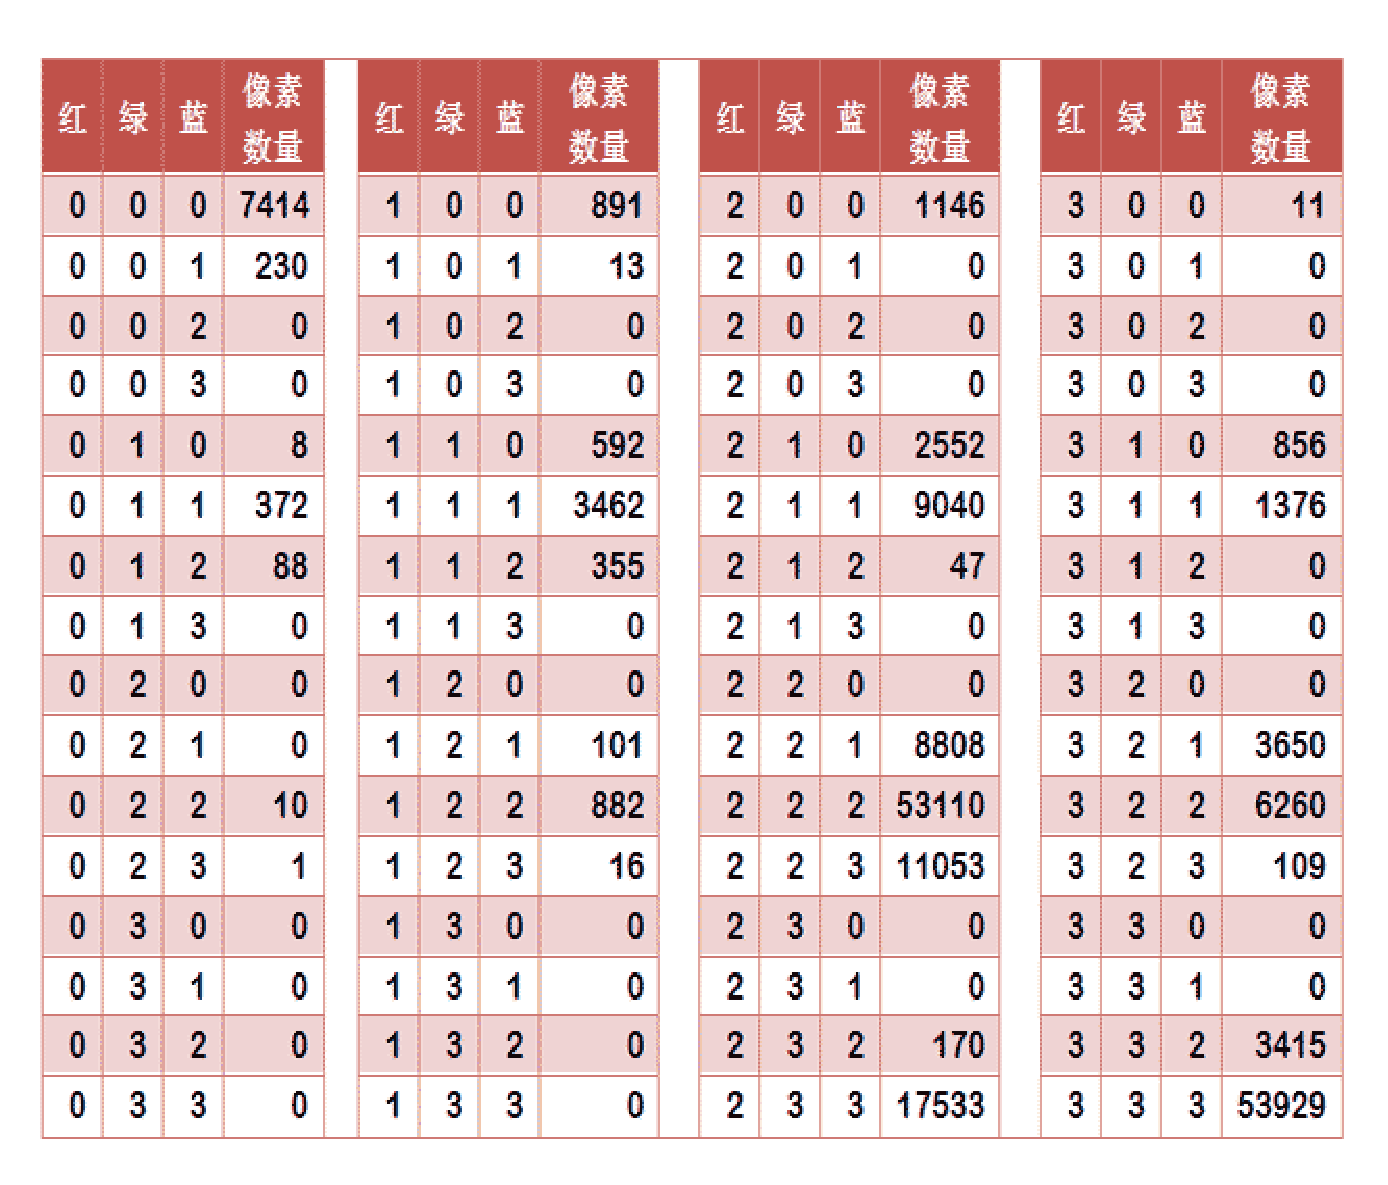
\includegraphics[width=0.95\textwidth]{figures/colordistribution.eps}
  \caption{颜色分布图}\label{fig:colordistribution}
\end{figure}

\section{大津阈值法}
图片处理中最常用的方法是将图片转换成较小的灰度图片,比如$50\times 50$,然后,再将灰度图片转成黑白图片(0-黑色,1-白色)。最终,使用0-1矩阵做相似性判断。在图片由灰度图片转换到黑白图片时,阈值选择是一个重要的步骤。

一般地,如果两张图片相似,那么它们的黑白轮廓自然也相近,一个合理的阈值应该能够正确呈现出图片的黑白轮廓,而反映轮廓清晰程度的重要因素是前景色与背景色的反差,反差越大则轮廓越明显。这就意味着,通过最小化前景色和背景色各自的类内差异(minimizing the intra-class variance),或者最大化类间差异(maximizing the inter-class variance)就可以找到理想的阈值$\theta$。

1979年,日本学者大津展之证明“类内差异最小”与“类间差异最大”是等价的,对应相同的阈值,这种通过最优化类内或类间差异,确定最佳阈值的简单方法就是大津阈值法(Otsu's thresholding method)。

假定一张图片共有$n$个像素,其中灰度值小于$\theta$的像素有$n_1$个,大于等于$\theta$的像素有$n_2$个,那么由此可以计算两种像素的权值$\omega_1 = n_1/n$和$\omega_2=n_2/n$。

再假定所有灰度值小于$\theta$的像素的平均值和方差分别为$\mu_1$和$\sigma_1$,所有灰度值大于等于阈值的像素的平均值和方差分别为$\mu_2$和$\sigma_2$,那么,可以计算类内差异和类间差异:
\begin{eqnarray}
  V_r &=& \omega_1\sigma_1^2 + \omega_2\sigma_2^2 \\
  V_e &=& \omega_1\omega_2(\sigma_1 - \sigma_2)^2
\end{eqnarray}
可以证明,两个等式是等价的,不过,从计算难度看,后者的计算要容易一些。

有了$50\times 50$像素的黑白缩略图,就等于有了一个$50\times 50$的0-1矩阵。矩阵的每个值对应原图的一个像素,0表示黑色,1表示白色。两个特征矩阵的不同之处越少,说明两张图片越相似。

\section{VisualRank}
在2008年北京国际万维网会议上,Google的两名科学家Yushi Jing和Shumeet Baluja介绍了一种图片搜索新型算法VisualRank,它通过直接分析图片内容,并充分利用图片名称、网络链接地址或者其他文本内容,寻找和排列图片。综合了图像识别、相似图像排序技术,应用到大规模图像搜索~\cite{jing2008visualrank}。

\chapter{基于评分的排名模型}
\section{牛顿冷却定律}
根据\textbf{牛顿冷却定律}(Newton's law of cooling)
\footnote{\href{http://www.ruanyifeng.com/blog/algorithm/}{阮一峰:算法与数学}},
“物体温度的变化速率正比例于物体同周围环境的温差”。%(The rate of change of the temperature of an object is proportional to the difference between its own temperature and the ambient temperature.)
假设在时刻$t$,物体温度是$T_t$,周围环境的温度不变,记为常量$T_{env}$,则冷却定律可以表示为微分形式
\begin{equation}
    T'_t = -\alpha(T_t-T_{env})
\end{equation}
其中,$\alpha>0$表示物体冷却系数。若以某个时点,如$t_0$为起始时刻,物体的初始温度为$T_0$,解微分方程可以得到物体温度随时间变化的规律
\begin{equation}
    T_t = T_{env} + (T_0 - T_{env})e^{-\alpha(t-t_0)}
\end{equation}

假设所有物体最终都会“冷寂”,环境温度等于0,就有
\begin{equation}
    T_t = T_0 e^{-\alpha(t-t_0)}
\end{equation}

对于新闻或博客,用户的点击、文章质量、文章发布距离现在的时间间隔(简称“年龄”)等属性是影响文章排名的重要因素。牛顿冷却定律(又称指数衰减规律)可以很好地体现时间对文章排名的影响:时间会降低文章的权重。系统首先为每篇文章赋予一个初始“温度”,随着文章年龄的增长,指数形式地降低文章的热度,其中冷却系数反映了物体温度变化的剧烈程度,如果希望文章热度变化缓慢,则可以选择比较小的$\alpha$,否则增大$\alpha$。

\section{HNRating}
2007年,创业孵化器Y Combinator的创始人Paul Graham
\footnote{Paul Graham,1964年生于英国,康奈尔大学本科、哈佛大学计算机科学博士,全球知名的程序员,风险投资专家,享有硅谷创业教父之美誉。1995年,他与麻省理工学院计算机教授Robert Morris 共同开发出世界上第一个互联网应用程序Viaweb,帮助个人用户在网上开店。1998年,Yahoo!公司以5,000万美元的价格收购Viaweb。
2005年他和Jessica Livingston(2008年两人结婚)联合创立Y Combinator孵化器。如今,YC 孵化器已经成为全球最出名的技术创业孵化器,已经成功孵化841家创业公司,包括Dropbox、Heroku、Airbnb、Bump、Justin.tv、Reddit、Disqus、Posterous 等明星公司,这些创业公司总计获得72亿美元的融资。}
创建Hacker News
\footnote{Hacker News: \href{http://thehackernews.com/}{http://thehackernews.com/}},
主要发布创业公司和骇客题材的社会化新闻。每条新闻(帖子)前都有一个上三角图形,如果用户觉得内容很好,可以点击一下,投上一票。系统根据得票数,会自动统计出热门新闻排行榜。但是,得票并非决定新闻排名的唯一因素,另外一个重要因素是时间,从而新闻要比旧闻获得更高的排名。系统新闻排序模型可以归结为用户投票与新闻年龄的函数,新闻的排名分值$S$可以表示为
\begin{equation}
   S = \frac{P-1}{(T+2)^G}
\end{equation}
其中,$P$是新闻的得票数目,减去1则忽略作者的投票。$T$是新闻发布距离现在的时间(以小时计)。$G$是重力因子(gravity),默认设置为1.8。重力因子越大,则旧帖子下沉的速度越快。

\section{Reddit热度评分}% Hot Rating
2005年6月,在接受 Y Combinator 的种子资金后,Alexis Ohanian 和 Steve Huffman 共同创立了 Reddit
\footnote{Reddit: \href{https://www.reddit.com/}{https://www.reddit.com/}}。
Reddit现已发展成为美国最火的社交新闻网站。2005年12月8日开始,Reddit社区用户可以评论帖子并投票:好评或差评,系统会根据得票数,更新“热贴排行榜”。

给定贴在发布时间$A$,可以计算距离Reddit评论功能开放时间点“$B=\text{2005年12月8日7:46:43}$”的间隔(以秒计)$t_s = A - B$,统计用户的投票结果,可以计算帖子好评数$U$与差评数$D$的差值$x=U-D$。Reddit根据帖子票差和年龄给帖子评分
\begin{equation}
    S = \log y + \frac{z t_s}{45000}
\end{equation}
其中,$y=\max\{|x|,1\},z=\sgn x$,对数函数取10为底。

分析评分公式的第一部分可以发现,帖子的得票票差越大(大多数用户观点一致),则帖子的得分越高,它不考虑投票的先后顺序影响。如果帖子富有争议,导致票差微小,则得分小于观点一致的帖子。假设两个同时发布的帖子,一个得分$U_1=10000,D_1=10001$,另一个得分$U_2=10,D_2=0$,前者得分为0,后者得分是1,整体来看,Reddit 推崇和谐社区建设,观点激进或少数派的帖子不太可能“榜上有名”。对于评分公式的第二部分,好评数大于差评数时,则新颖性会给帖子加分,反之,如果差评数高于好评数,那么新颖性会给帖子减分。目前,Reddit已经启用新的评论排名算法
\footnote{\href{http://jandan.net/2014/04/03/reddits-comment-sorting.html}{Reddit 的评论排序新算法}}。

\section{Reddit最佳评分}% Best Rating
基于用户投票进行排名的系统通常会犯两种类型的错误,使用“好评与差评的差值”或“好评率”对物品排名。第二种错误不是那么明显,假设用户对两个帖子的评价一个是$U_1=1, D_1=0$,一个帖子的评价是$U_2=95, D_1=5$,显然第一个帖子的好评率(100\%)大于第二个贴子(95\%)。从直观来看,根据好评率进行排序不合理。

假设每个用户的评价(好评或差评)都是一个独立随机事件,服从参数为$\hat{p}$的二项分布,好评率$p$是参数$\hat{p}$的一种估计。在统计学中,人们常使用置信区间估计真实参数的取值范围。使用相同的置信度$1-\alpha$,置信区间的宽度越小则表明参数估计越可信。比如,一个帖子有8个好评,2个差评,另一个帖子有80 个好评,20 个差评。两个帖子的好评率都是80\%,但是前者的置信区间是[70\%, 90\%],后者是[75\%, 85\%]。第二个置信区间比第一个置信区间窄,其置信区间的下限值更大,那么它的排名应该靠前。

对于大样本数据($np > 5,~~n(1 - p) > 5$),根据中心极限定理,二项分布的置信区间可以利用正态近似区间计算$\hat{p}\pm z\sqrt{\hat{p}(1-\hat{p})/n}$,在小样本数据上,其准确性较差。1927年,Edwin Wilson\cite{wilson1927probable}修正正态近似区间,提出Wilson区间公式
\begin{equation}
  \frac{1}{1 + z^2/n} \Big[\hat p + z^2/(2n) \pm z \sqrt{\hat p (1 - \hat p)/n + z^2/(4n^2)}~~\Big]
\end{equation}
用于处理小样本数据样本上的参数估计问题。$z$表示标准正态分布的$1-\frac{1}{2}\alpha$分位数,对于置信度$1-\alpha=0.95$,错误率为$\alpha=0.05$,则标准正态分布的$0.975$分位数等于$1.96$。Reddit使用\textbf{Wilson区间下界}给社区中的评论打分,下界越大评分越高
\begin{equation}
    S = \frac{1}{1 + z^2/n} \Big[~~\hat p + z^2/(2n) - z \sqrt{\hat p (1 - \hat p)/n + z^2/(4n^2)}~~\Big]
\end{equation}
如果选择分位数$1-\frac{1}{2}\alpha=0.975$,则有
\begin{equation}
    S = \frac{1}{1 + 3.8416/n} \Big[~~\hat p + 1.9208/n - 1.96 \sqrt{\hat p (1 - \hat p)/n + 0.9604/n^2}~~\Big]
\end{equation}

\section{Stack Overflow评分}
2008年,Jeff Atwood与Joel Spolsky创建了Stack Overflow
\footnote{Stack Overflow: \href{http://stackoverflow.com/}{http://stackoverflow.com/}},
目前是世界上最受欢迎的程序员问答社区。Stack Overflow 根据浏览量$n_v$,回答人数$m$,回答的质量评分$s_i,i=1,\ldots,m$,其他用户对问题好评与差评差值$e$,问题发布年龄$t_a = t-t_0$,最后一次更新时间$t_u = t-t_m$,对用户提交的问题评分:
\begin{equation}
    S = \frac{4 \log n_v + m e/5 +\sum\limits_i s_i}{\big[0.5(t_a + t_u + 2)\big]^{1.5}}
\end{equation}

\section{IDMb榜首250评分系统}
IMDb(Internet Movie Database)
\footnote{IMDb: \href{http://www.imdb.com.cn/}{http://www.imdb.com.cn/}}
是全球最大的一个电影资料库,包括几乎所有的电影及1982年以后的电视剧作。IMDb资料库包含影视作品、演员、电游资料及分级、评论数据,评分采用10分制,其使用的评分体系是目前最流行的电影评分系统。

IMDb根据真实贝叶斯估(true bayesian estimate)计算电影评分
\begin{equation}
    S = \frac{v}{v + m} \bar S + \frac{m}{v + m} C
\end{equation}
将排名前250的电影放到首页。电影的评分$S$是其基于当前数据库中所有电影的平均得分$\bar S$与平滑常量$C$(当前7.0)的加权平均,$v$表示电影当前的投票总数,$m$表示电影有资格进入前250榜单的最低得票数(当前25,000)。


\begin{shaded}
现代搜索引擎是一种检索互联网信息的应用程序,主要包括三个模块:采集信息、建立索引、检索信息。搜索引擎是传统信息检索的一个重要应用,它使用计算机程序(网络爬虫或蜘蛛)自动采集互联网数据,然后对采集到的信息进行合理组织与处理(去重、索引等),根据前台搜索界面接收到的用户检索需求,即时迅速地从采集数据中检索到相关文档,并按照相关程度由高到低以列表的形式反馈给用户。搜索引擎肇始于20世纪末的加拿大,经过20多年的迅猛发展,已经成为人们获取信息的一个重要手段。

1990年,加拿大McGill大学的Alan Emtage、Peter Deutsch与Bill Wheelan联合开发出的一种在线FTP文件索引工具\textbf{Archine},堪称世界首个搜索引擎。它汇集上百个计算机系统的FTP文件资源生成一个文件目录,用户可以使用Unix grep命令查询文件名,从而确定存储目标文件的计算机系统。1992年,Nevada大学的Steven Foster与Fred Barrie出于相同目的开发出\textbf{Veronica},用于搜索普通文本文件。1993年,Utah大学的Rhett Jones与Veronica目标同又开发出\textbf{Jughead}。Veronica与Jughead均受到Archine的影响,分别通过Archine Comic的两个经典漫画人物Veronica Lodge与Jughead Jones向Archine致敬,并且二者发送文件均是基于Gopher系统。

1993年6月,MIT大学的Matthew Gray期望能够追踪互联网发展速度,于是就创造出了世界上第一个网络爬虫程序万维网\textbf{Wanderer},更新以后爬虫程序能够获取真实的网址。爬虫程序每天访问同一个网页上百次,严重影响互联网的速度,人们开始质疑其用处。1993年10月,Martijn Koster开发出\textbf{ALIWEB}(Archie-Like Indexing of the Web)。ALIWEB只抓取少量网页元信息的,允许用户自己提交期望能被索引到的网页数据,如此可以节省大量的带宽资源。对于Wanderer,ALIWEB代表一种强有力的回应,遗憾的是许多人不知如何提交自己的网站。截至1993年12月,陆续又涌现出三个基于网络爬虫的搜索引擎:Scotland的\textbf{JumpStation}、Colorado大学Oliver McBryan的\textbf{万维网蠕虫}、NASA的\textbf{RBSE}(Repository-Based Software Engineering)爬虫。JumpStation采集网页的标题与头部信息,并使用简单的线性搜索执行检索。互联网数目的不断增长最终将JumpStation淘汰出局。万维网蠕虫对网页标题信息及URL建立索引,但是它与JumpStation一样,对检索到的网页一视同仁按照顺序进行排列。RSBE爬虫则实现了一个排序系统,但没有意识到链接分析或者网页内容缓存的重要性。如果用户无法提供确切名称,系统仍然难以找到目标文件。

1993年2月,斯坦福大学六名学生Graham Spencer、Joe Kraus、Mark Van Haren、Ryan Mc Intyre、Ben Lutch和Martin Reinfried成立Architext项目,意图利用字词间关系的统计分析提升搜索效率。1993年6月,他们发布了开发的搜索软件\textbf{Excite}用于网络搜索。1999年1月,@Home以65亿美元的价格收购Excite,并易名为Excite@Home。2001 年10月,Excite@Home破产,InfoSpace以1000万美元的价格将其买下。2002年5月,Excite停止使用自己的搜索引擎,改用元搜索引擎Dogpile。

1994年1月,世界上第一个提供分类目录和搜索功能的\textbf{EINet Galaxy}上线。1994年4月,斯坦福大学博士生Jerry Yang与David Filo共同创办\textbf{Yahoo!}用于收集它们喜欢的网页。随着收录数目与访问量的增加,Yahoo!开始支持简单的数据库搜索。由于Yahoo!收录的网页需要经过手工处理,算不上真正意义的搜索引擎。Yahoo! 陆续采用Altavista、Inktomi、Google提供的搜索引擎服务,推动了搜索引擎技术的发展。1994年4月20日,华盛顿大学的Brian Pinkerton发布
\textbf{WebCrawler},它是世界上第一个支持全文检索的搜索引擎。1994年7月20日,卡内基梅隆大学的Michael Mauldin研发的\textbf{Lycos}正式发布,它是搜索引擎发展史上的一次革命,不仅提供相关性排名,还支持前缀匹配与单词近似匹配,也是第一个在搜索结果页面中实现网页自动摘要,并且它的数据量远超其他搜索搜索引擎。1999年4月,Lycos改由Fast提供搜索引擎服务。1994年底,又一个重要的搜索引擎\textbf{Infoseek}发布。Infoseek友善的用户界面、大量附加服务使它声望日隆。而1995 年12月与Netscape 的战略性协议,使它成为一个强势搜索引擎:当用户点击Netscape浏览器上的搜索按钮时,弹出Infoseek的搜索服务,而此前由Yahoo! 提供该服务。2001 年2 月,Infoseek改用Overture的搜索结果。

1995年,华盛顿大学的Eric Selberg 和 Oren Etzioni开发出\textbf{MetaCrawler},成为世界首个元搜索引擎。元搜索引擎对用户的检索请求进行转换处理,按照格式要求提交给多个成员搜索引擎,最终将所有成员搜索引擎的搜索结果进行汇总并反馈给用户。1995年12月,\textbf{AltaVista}发布亮相,它推陈出新提供大量的创新服务,迅速成为搜索领域的一支新秀。它是第一个支持自然语言搜索、第一个支持高级搜索语法(如AND,OR,NOT 等)、并声称是第一个支持用户自主提交或删除网站网址,并保证24小时内可以检索到的搜索引擎。1995年9月26日,加州伯克利大学的Eric Brewer、Paul Gauthier联合创立\textbf{Inktomi}。1996年5月20 日,Inktomi公司正式成立,并发布新的搜索引擎\textbf{HotBot}。Inktomi公司声称HotBot每天抓取的网页数目超过1000万,远超其它搜索引擎。Hotbot成为随后几年最受欢迎的搜索引擎之一。

1998年9月4日,斯坦福大学的Larry Page与Sergey Brin联合成立\textbf{Google}公司。2004年8月19日,在纳斯达克上市。由于技术先进,经过短短十多年的发展,Google 已经成为全球最大的搜索引擎,搜索服务覆盖全球30多种语言、100多个国家。

1997年,挪威科技大学的Tor Egge成立FAST(Fast Search \& Transfer)公司,1999年5月发布搜索引擎\textbf{AllTheWeb}。FAST试图复制Inktomi的模式,向其他搜索引擎提供数据。它宣称在数据的新颖性、高级搜索功能、搜索结果聚类、本地化显示、图片搜索方面都比Google更具优势。2003年2月,FAST网络搜索部门被Overture 收购。2004年3月25日,Overture被Yahoo!收购。2011年4月4日,alltheweb.com网站重定向到Yahoo!搜索。

2000年,Rutgers大学的Apostolos Gerasoulis及其同事创立\textbf{Teoma},2001年春正式上线。2001年9月11日被Ask Jeeves以大约400万美元的价格收购,为ask.com提供搜索服务。Teoma排名算法ExpertRank比较独特,它同时基于主题分类、链接分析给网页排名。2000年,前Infoseek工程师Matt Wells创立\textbf{Gigablast},索引了2 亿多网页,向合作网站提供大规模高性能的实时信息检索服务。目前,Matt Wells是Gigablast唯一的维护人员,并于2013年7月将代码开源托管到GitHub。2000年5月16日,Yeogirl Yun创立\textbf{WiseNut},并于2001年9月正式上线。WiseNut引进一种新型数据库,并发明一种新技术WiseGuide实现对搜索结果自动聚类,但是对高级搜索、布尔查询、网页快照等功能它却视而不见。2002年4月,被分类目录提供商LookSmart以900万美元的价格收购,试图成为主流搜索引擎。

1997年10月29日,北京大学“网络与分布式系统”研究室研发的“\textbf{天网}”中英文搜索引擎系统正式在CERNET上提供服务。它是国家“九五”重点科技攻关项目“中文编码和分布式中英文信息发现”的研究成果,提供北京大学、中国科院等FTP站点的检索。2000年初,在国家973重点基础研究发展规划项目基金资助下成立“天网”搜索引擎课题组,继续为天网提供技术支持。1998年1月,\textbf{Openfind}创立,并由台湾中正大学吴升教授领导的GAIS实验室提供技术支持。Openfind是当时最好的中文搜索引擎,鼎盛时期同时为三大门户网站新浪、奇摩、雅虎提供中文搜索服务。2002年6月,Openfind重新发布基于GAIS30工程的Openfind搜索引擎Beta版,推出多元排名(PolyRank)算法,宣布累计抓取网页35亿,并踏入英文搜索领域。2000年1月18日,超链分析专利发明人、前Infoseek资深工程师李彦宏(Gigablast的创始人Matt Wells是其在Infoseek的同事)与UC Berkeley大学博士徐勇联合创立\textbf{百度}公司。2000 年6 月,百度正式推出独立搜索门户baidu.com,并开始为多个门户网站(如搜狐、新浪、雅虎中文等)提供搜索服务。2001年10月22日正式发布Baidu搜索引擎。2005 年,百度在美国纳斯达克上市,成为首家进入纳斯达克成分股的中国公司。百度提供了音乐、视频、图片、百科、文库等各种搜索服务,成为目前全球最大的中文搜索引擎。
\end{shaded}%---------------information retrieval
\part{排名理论}

%\ornamento
\chapter{社会选择理论}
人类行为是由一系列选择(choice)和决策(decision making)构成,理解人类行为的一切思想都以研究选择为基础,如古希腊先哲苏格拉底(Socrates)和亚里斯多德
(Aristotle)认为愿望和信仰是人类做出选择的前提。19世纪,人们开始构建人类选择的量化模型,比如实验心理学的奠基人恩斯特·海因里希·韦伯Ernst Heinrich Weber 通过建立心理活动和可度量物理行为间的关联,提出著名的\textbf{韦伯定律},成为心理学量化分析人类心理活动(包括选择)的基石。承其衣钵的学生古斯塔夫·费希纳Gustav Theodor Fechner扩展韦伯定律,创立出更为精确的度量系统,称作\textbf{费希纳定律}。20世纪初,法国路易斯· 列昂· 瑟斯顿Louis Leon Thurstone
\footnote{路易斯· 列昂· 瑟斯顿Louis Leon Thurstone(1887-1955),美国心理学家,美国心理测量学会的创立者之一,并任第一届心理测量学会主席,在测量理论、社会评价等理论应用方面均作出巨大贡献。1933年当选为美国心理学会主席,1938年当选为国家科学院院士。}
基于韦伯--费希纳定律发展出比较性评价(comparative judgment)系统~\cite{thurstone1927method},基于成对比较的瑟斯顿模型由此诞生。

社会选择(social choice),也称“集体决策”(collective decision)是将社会成员的个人意愿或偏好汇集成群体意愿或偏好的过程,属于典型的群体决策问题。选举制度是社会选择的一个制度性体现,为民主国家反映民意的一个主要机制。为了体现少数服从多数的民主理念,人们提出\textbf{多数代表制}(majoritarian representation)或\textbf{多数制}(plurality voting),认定得票最多的候选人胜出。为了确保反映社会多元化的意见,1846年瑞士学者Victor Considerant提出
\textbf{比例代表制}(proportional representation),根据政党或参选组别得票比例分配议席。由于不同选区人口或经济地位的差异,人们根据每个选区所代表的议席数目,将选举方法分成\textbf{单一选区制}(single-member district)或“小选区制”(small constituency system)、\textbf{复数选区制}(multi-member district)或“大选区制”(large-size district)。单一选区制每个选区只有一个议席,而复数选区制每个选区对应多个议席。多数制在单一选区制下也称作\textbf{简单多数制}(first-past-the-post, single choice voting, simple plurality, simple majority)或\textbf{相对多数制}(relative majority)
\footnote{多数制别称相对多数制,与之对应的是绝对多数制(absolute majority):候选人得票数只有超过其他候选人得票数之和才算胜出。};在复数选区制下称作
\textbf{胜者全拿}(winer-takes-all)。如果根据选举规则无法选出一个合适的候选人,可能是平局,也可能是不满足一定的规则,为避免出现此类状况,人们提出
\textbf{决胜选举}(run-off)进行多轮投票直至有人胜出。

我们将在后续章节介绍社会选择的相关概念、公理性推导、社会选择方法与投票准则、评价社会选择的标准、各种社会选择方法的关联以及几个著名的社会选择悖论,最后介绍社会选择理论最新进展\textbf{计算社会选择}(Computational Social Choice,CSC),以及社会选择理论在推荐系统评分预测、网络排名聚合、体育竞技排名等领域的应用研究。

\section{符号定义}
社会选择通常依赖于可排列对象的排列变换(permutation)
\footnote{英文单词Permutation存在两个中文字面翻译:\textbf{排列}或\textbf{置换}。本文对两种翻译不作具体区分,主要使用第一种翻译意思。当permutation作为一个变换算子出现时,我们称其\textbf{排列变换};当permutation作为一个有序列表出现时,我们称其\textbf{排名列表}。读者如果对排列和置换之间的差异感兴趣,可参考潘庆年教授的一篇注解\cite{pan1998note}。},为此我们对相关概念给出统一的数学定义。假设$\mathcal A = \{x,y,z,\ldots\}$是可排序
\footnote{可排序依赖于空间上定义的二元全序关系,我们将在后文给出严格定义。}
的对象集,如决策时的备择选项(alternatives)、选举投票时的候选人集合(candidates)、在线购物评分时的商品列表(items)等,并且$|\mathcal A|=n$,$\mathcal A$上的一个\textbf{排列}(ranking \textit{or} ballot)定义为从$\mathcal A$ 到$\{1,2,\ldots,n\}$上的一个双射:
\begin{equation}\label{eq:permutation}
    \pi: \mathcal A \mapsto \{1,2,\ldots,n\},
\end{equation}
并使用$\pi(i)$表示$\mathcal A$中第$i$个对象在排列变换$\pi$作用下的排名,$\pi^{-1}(i)$表示在$\pi$作用下排在第$i$位的原始对象。通常,我们也使用$\pi$和$\pi^{-1}$ 分别表示由$\mathcal A$中所有对象的排名向量、有序排列的对象向量。对象集$\mathcal A$可以产生$n!$种可能的全排列组合,可以构成一个非交换群,记为$\Pi[\mathcal A]$或$\Pi[n]$。 如果我们选择一部分对象,比如$\{\pi^{-1}(1), \pi^{-1}(2), \ldots, \pi^{-1}(K)\}$,从群$\Pi[n]$中筛选出所有第$i$ 位对应$\pi^{-1}(i)$ 的排列,$1\le i\le K \le n$,构成$\Pi[n]$ 的一个子群,记作$\Pi[n,K, \pi]$:
\begin{equation}\label{eq:subgroup}
    \Pi[n,K,\pi] = \big\{\sigma\in \Pi(n)|\sigma^{-1}(i) = \pi^{-1}(i), 1\le i \le K\big\}.
\end{equation}
假设存在一组决策者$\mathcal M=\{X,Y,Z,\ldots\}$,比如投票选举时的选民(voters)、电影评价时的影评人(raters)等,并且$|\mathcal M|=m$,每个决策者都有一个$\mathcal A$上的个人偏好排名(individual preferential ranking),从而构成一个\textbf{社会偏好集}(social preference profile)
\begin{equation}\label{eq:preferenceprofile}
    \Pi[\mathcal A,\mathcal M]=\Pi[n,m]=\{\pi_i\}_{i=1}^m\in  \Omega[n,m],
\end{equation}
其中$\pi_i\in \Pi[n]$表示$\mathcal M$上第$i$个决策者对$\mathcal A$ 做出的一个线性排序,$\Omega[n,m]$是$\mathcal M$在$\mathcal A$上所有可能的偏好集,且有$|\Omega[n,m]|=(n!)^m$。在不产生混淆的情况下,我们简记作$\Pi\triangleq \Pi[n,m]$。 如果存在一个社会选择函数$\mathcal F: \Pi[n,m]\mapsto \Pi[n]$,能够基于$\Pi[n,m]$ 给出$\mathcal A$ 的一个全局性的评价,则全局线性排序记作$\pi_{\mathcal F}\in \Pi[n]$,也成社会偏好排名(social preferential ranking)。 对于任意一个$\mathcal A$上的线性序$\pi$,都对应一个特殊的决策方。给定任意两个对象$x,y\in \mathcal A$,我们用$x\succ_\pi y$ 表示$x$ 在$\pi$中的排名高于$y$,或者$\pi$偏好$x$甚于$y$。为了强调决策方,比如决策者$Z$偏好$x$甚于$y$,则记作$x\succ_Z y$。如果$\mathcal F$ 偏好$x$甚于$y$,则记作$x\succ_{\Pi[n,m]}^{\mathcal F} y$,或简记作$x\succ_\Pi^{\mathcal F} y$。如果存在一个社会选择函数$\mathcal F:\Pi[n,m]\mapsto \mathcal A$,则它能够基于$\Pi[n,m]$选择$\mathcal A$上的一个成员,并称其为社会选择(social choice)。我们根据大量决策者的偏好信息,从而确定出$\mathcal A$中的一个成员或者全体社会对$\mathcal A$的整体偏好。如果细分两种情形,则前者对应一个社会选择函数$\mathcal F: \Pi[n,m]\mapsto \Pi[n]$;后者对应一个社会福利函数$\mathcal F: \Pi[n,m]\mapsto \mathcal A$。
\begin{example}\label{eg:gallup-2016}
    2014年7月7日至10日,盖洛普(Gallup)对民主党五位2016年总统选举候选人Hillary Clinton、Elizabeth Warren、Andrew Cuomo、Martin O'Malley、Joe Biden组织了一次民意调查
    \footnote{Gallup: \href{http://www.gallup.com/poll/173402/clinton-best-known-best-liked-potential-2016-candidate.aspx}{\textit{Clinton Is Best Known, Best Liked Potential 2016 Candidate}}, 2015-09-14},
    统计公众对几位候选人的了解情况,具体统计数据见下表:
    \begin{table}[htbp]
        \centering
        \begin{tabular}{lcccc}
          \hline
          Candidate & Familiar (\%) & Favorable (\%) & Unfavorable (\%) & Net Favorable (\%)\\
          \hline
          Hillary Clinton & 91 & 55 & 36 & 19\\
          Elizabeth Warren & 38 & 21 & 17 & 4\\
          Andrew Cuomo & 51 & 27 & 24 & 3\\
          Martin O'Malley & 19 & 7 & 9 & -2\\
          Joe Biden & 80 & 38 & 42 & -4\\
          \hline
        \end{tabular}
        \caption{2014年7月7日至10日盖洛普民主党2016总统候选人民调数据}
        \label{tbl:gallup-2016}
    \end{table}
    表格中每一行代表一位候选人,第二列是公众认识候选人的比例,第三列是公众认同候选人的比例,第四列是公众不认同候选人的比例,最后一列则是公众认同候选人减去不认同的比例,属于净认同的比例。根据数据可知,五位总统候选人$\mathcal A=\big\{$Clinton,Warren,Cuomo,O'Malley,Biden$\big\}$中,美国前第一夫人、前国务卿Clinton是公众最为熟知、最受公众欢迎的民主党候选人。前副总统Biden虽为公众所知,认同他的民众却少于不认同他的人数。

    我们现在用一组连续的自然数$\{1,2,3,4,5\}$为他们编号,则1号对应Clinton,3号对应Cuomo。如果根据第二列的公众熟知比例为他们排名,则会产生一个新的排名列表$\pi_1=\langle 1, 4, 3, 5, 2\rangle$,那么$\pi_1^{-1}(4)=2$表示排名列表$\pi_1$中位列第4的对象是2号候选人Warren,$\pi_1(5)=2$表示5号候选人Biden 在列表$\pi_1$ 中排名第2 位。类似地,我们按照最后一列排列候选人名单,又会产生一个排名列表$\pi_4=\langle1, 2, 3, 4, 5\rangle$。
\end{example}

我们根据社会选择法的步骤及输出数据类型\cite{riker1982liberalism,farah2007outranking},将社会选择方法分成位置评分法、位置筛选法和概率模型法。位置评分准则赋予每个候选人一个对应分值,分值的产生可能源于整体排序(如波达计数\cite{borda1781m}、Footrule法\cite{marden1995analyzing}、中位数法
\cite{fagin2003efficient}、CPS模型\cite{qin2010new} 和矩阵分解方法\cite{gleich2011rank}),或者源于序对比较(如孔多塞法、凯梅尼─杨格方法和马尔科夫方法)。位置筛选法综合候选人的位置、多数投票得分等因素,逐步缩短偏好列表的长度,剔除不合格的候选人直至最优人选诞生,如单记可让渡投票制。概率模型法建立候选人排列的概率分布,包括瑟斯顿模型~\cite{thurstone1927method}、 布雷德利─特里模型~\cite{bradley1952rank}、 马洛斯模型~\cite{mallows1957non} 和普拉基特─卢斯模型~\cite{luce1959individual,plackett1975analysis}。我们在后续几个小节简要介绍几种代表性的社会选择方法,并基于1980年美国参议院议员选举为例解释各种方法。

\begin{example}\cite{taylor2008mathematics}
1980年美国纽约州参议院选举在保守派的Alphonse D'Amato、自由派的Elizabeth Holtzman与Jacob Javits之间展开,三名候选人的得票率如表\ref{tbl:1980ussenate}所示,22\%的选民对于三名候选人的个人偏好为$D\succ H\succ J$,4\%的选民存在个人偏好$J\succ D\succ H$,每名候选人使用其姓氏首字母表示。为简化表示,我们在后续章节使用本例数据时直接省略百分号。
\begin{table}[ht]
    \centering
    \begin{tabular}{c|c|c|c|c|c}
      \hline
      29\% & 23\% & 22\% & 15\% & 7\% & 4\%\\
      \hline
      H & D & D & H & J & J\\
      J & J & H & D & H & D\\
      D & H & J & J & D & H\\
      \hline
    \end{tabular}
    \caption{1980年美国纽约州参议院选举}
    \label{tbl:1980ussenate}
\end{table}
\end{example}\label{eg:1980usny}

\section{位置评分法}
位置评分法根据每个偏好列表对所有候选人评分,然后累加候选人在所有偏好集上评分得到总的分值,利用各候选人的综合评分可以选出优胜者或者建立所有候选人的综合排名。假设$V_\pi\in \mathbb R^n$表示$\mathcal A$在偏好列表$\pi$上的得分向量,则$\mathcal A$内所有候选人的综合得分向量
\begin{equation}
    V_\Pi=V_\Pi = \sum\limits_{\pi\in \Pi}V_\pi = \sum\limits_{\pi\in \Pi} \bigg(V_\pi^1,V_\pi^2, \ldots, V_\pi^n\bigg),
\end{equation}
其中$V_\pi^i$表示$\mathcal A$中第$i$个候选人在偏好列表$\pi$下的得分分值,$1\le i\le n$。

\subsection{多数投票法}
多数投票法是一种最常见的投票选择方法,也是英国大选采用的一种选举方法。它只利用所有偏好列表排名第一的数据确定出最终赢家。对于某个选民偏好列表$\pi$,根据候选人集合$\mathcal A$ 在偏好名单$\pi$上的名次,只有排名第一的候选人可以得到一个点数,其他位置上的候选人没有得分。对于例子\ref{eg:1980usny},多数投票法只考虑排名第一的候选人,各候选人的得分如下:
\[
    \text{$V_D$ = 23 + 22 = 45,$V_H$ = 29 + 15 = 44,$V_J$ = 7 + 4 = 11},
\]
候选人D'Amato以45比44险胜Holtzman,社会偏好为$D\succ H\succ J$。

\subsection{波达计数}
1770年,法国数学家、政治学家让─查尔斯·波达Jean-Charles de Borda\cite{borda1781m}设计出一种新的投票计数方法,称作\textbf{波达计数}(Borda Count),用于评选法国科学院院士。波达计数根据选民偏好名单中的排名给候选人一定的点数,一般地排名越高点数越高,如排名第一的候选人得到$n-1$个点,排名靠后依次逐渐减少一个点。后来,由于波拿巴·拿破仑的干预,弃用波达计数,并采纳拉普拉斯的意见,使用绝对多数准则评选科学院院士。根据波达计数法,例\ref{eg:1980usny}三名候选人得分
\[
    \begin{bmatrix}
        V_D\\
        V_H\\
        V_J\\
    \end{bmatrix} = 
    \begin{bmatrix}
      0 & 2 & 2 & 1 & 0 & 1\\
      2 & 0 & 1 & 2 & 1 & 0\\
      1 & 1 & 0 & 0 & 2 & 2\\
    \end{bmatrix}
    \times 
    \begin{bmatrix}
        \vspace{-0.3cm}
        \text{29}\\
        \vspace{-0.3cm}
        \text{23}\\
        \vspace{-0.3cm}
        \text{22}\\
        \vspace{-0.3cm}
        \text{15}\\
        \vspace{-0.3cm}
        \text{7}\\
        \vspace{-0.3cm}
        \text{4}\\
        \vspace{-0.3cm}
    \end{bmatrix} =
    \begin{bmatrix}
        \text{109}\\
        \text{115}\\
        \text{74}\\
    \end{bmatrix},
\]
可知候选人Holtzman胜出,社会偏好为$H\succ D\succ J$。

\subsection{计分投票法}
多数投票法与波达计数都是建立在排序投票系统之上,选民只是根据自己的偏好对候选人进行排列。实际上,如果选民能够对候选人进行顺次排序,我们可以给予其更多的自由,使用限定的离散分值给候选人打分,从而能够更有效地反映出选民的意愿。这种投票选举的方法称作\textbf{计分投票法}(range voting,rating summation,scoring),在网络空间有广泛应用,比如网民对电影、图书、商品的1--5级评分。计分投票法根据每个候选人所有评分均值、中值(majority judgment)或加和,评分最高者胜出。如果离散分值只有两个$\{0,1\}$或者$\{$同意,反对$\}$,则称计分投票法为\textbf{同意投票法}(approve voting)。我们可以从计分投票中构建每个选民的偏好排名,允许一对一的对决,满足各种良好的性质,如传递性、一致性等。可以如果存在策略性投票行为,由于每张选票每个候选人的可能分值是一个区间范围,即便是离散数字,也比排名列表形式的选票更难操纵。

\subsection{孔多塞方法}
1785年,法国启蒙思想家马奎斯·孔多塞Marquis de Condorcet\cite{condorcet1785essai}在研究民主决策时,提出一种序对型选举投票方法,称为\textbf{孔多塞方法}。孔多塞方法根据选民的偏好集合$\Pi$,统计所有可能的偏好序对,根据多数准则选出得票最多的赢家。如果$\Pi$存在一个候选人(比如$x$),在和其他每个候选人一对一对决(round-robin \textit{or} one-on-one \textit{or} head-to-head)
\footnote{体育运动竞技比赛,如网球、足球、国际象棋、桥牌、拳击运动,经常要运动员或团队之间进行多轮形式的循环赛(\textit{round-robin tournament}),表示所有参赛选手彼此进行多次两两对决。17世纪初,\textit{round-robin}衍生出新的涵义,表示“圆形签名请愿书”。在签署控诉书、请愿书等多人署名文件时,顺着一个圆圈署名,籍此让人分不出署名的先后顺序,以保护领头人免于遭受报复。}
时,都能获得多数选票,即有
\begin{equation}
    \forall y \in \mathcal A,~~\big|\{\pi\in \Pi: x\succ_\pi y\}\big| > \big|\{\pi\in \Pi: y\succ_\pi x\}\big|\text{,或} x\succ_\Pi^\mathcal{F'} y\text{,}
\end{equation}
则称其\textbf{孔多塞赢家}(Condorcet winner),其中$\mathcal{F'}$是多数投票法。根据孔多塞方法,例子\ref{eg:1980usny}中三个候选人的一对一对决统计结果如表\ref{tbl:condorcetwinner} 所示,候选人Holtzman是一个孔多塞赢家,并且社会偏好为$H\succ D\succ J$。
\begin{table}[ht]
    \centering
    \begin{tabular}{c|c|c}
      \hline
      偏好 & 得票 & 偏好\\
      \hline
      $H\succ D$ & 51 $>$ 49 & $D\succ H$\\
      $H\succ J$ & 66 $>$ 34 & $J\succ H$\\
      $D\succ J$ & 60 $>$ 40 & $J\succ D$\\
      \hline
    \end{tabular}
    \caption{孔多塞赢家}
    \label{tbl:condorcetwinner}
\end{table}
如果一个候选人是$\Pi[n]$上的孔多塞赢家,则它在一对一对决中从未被其他候选人击败,即是说其他每个候选人至少被此孔多塞赢家所击败一次,他们不可能是孔多塞赢家。由此可知,孔多塞赢家只要存在必然唯一,但它并非总是存在。
\begin{example}
假设某次社会投票选举只有三个候选人$\{x,y,z\}$参选,他们的偏好集如表\ref{tbl:condorcetsparadox}所示。根据孔多塞方法,统计每个候选人一对一对决结果,比如有20个选民存在偏好$x\succ y$,只有10个选民有偏好$y\succ x$,前者得两票胜出,则$x\succ y$;类似可知$y\succ z$与$z\succ x$。孔多塞方法在此社会偏好集上产生一个偏好回路(preferential cycle)$x\succ y\succ z\succ x$,存在一个内在矛盾:社会偏好$x$甚于$y$,偏好$y$甚于$z$,但又偏好$z$甚于$x$,孔多塞赢家并不存在,出现孔多塞悖论(Condorcet's paradox)。
\begin{table}[ht]
    \centering
    \begin{minipage}[t]{0.3\linewidth}
    \centering
    \begin{tabular}{c|c}
      \hline
      票数 & 偏好列表\\
      \hline
      10 & $x\succ y \succ z$\\
      10 & $y\succ z \succ x$\\
      10 & $z\succ x \succ y$\\
      \hline
    \end{tabular}
    \end{minipage}
    \begin{minipage}[t]{0.3\linewidth}
    \centering
    \begin{tabular}{c|c|c}
      \hline
      偏好 & 票数 & 偏好\\
      \hline
      $x\succ y$ & 20$>$10 & $y\succ x$\\
      $y\succ z$ & 20$>$10 & $z\succ y$\\
      $z\succ x$ & 20$>$10 & $x\succ z$\\
      \hline
    \end{tabular}
    \end{minipage}    
    \caption{孔多塞悖论}
    \label{tbl:condorcetsparadox}
\end{table}
\end{example}

孔多塞在分析投票方法时还给出一个著名的\textbf{孔多赛陪审团定理}(Condorcet's Jury Theorem):“如果每个陪审员做出正确决定的概率都大于$0.5$,那么陪审员越多,则陪审团做出正确决定的可能性就越大。当陪审员达到一定规模,陪审团做成正确判决的概率会无限趋近于$1$”。

当法庭作出某项审判决定时,陪审团按照多数准则进行表决,只有当表决赞同或反对法庭审判决定的陪审员达到一定比例,陪审团同意或否决法庭判决的决议才能生效。孔多塞陪审团定理假定“每个陪审员都能独立做出决定,赞同或否决法庭判决,并且做出正确决定的概率相同”
\footnote{公元前399年,70岁的苏格拉底由于被指控不敬神和败坏青年而站到雅典的法庭上,一个由501名公民构成的陪审团在第一轮投票以280对221的微弱优势判处苏格拉底有罪,在第二轮以360对141的多数优势判其死刑,陪审团通过民主的程序将激怒他们的苏格拉底处死。西德尼·吕美特执导的《十二怒汉》(12 Angry Men)告诉我们“陪审员独立作出决定”是一种理想化的设定,可能促成陪审团做出正确的决定或相反,多数同意准则不一定就是民主的、永远有效的表决方案。}。
我们现在从概率统计的角度进行分析,设陪审团由$n$名陪审员组成,每个陪审员\textbf{独立做出正确决定}的概率是$p$,则整个陪审团能否做出正确判决取决于多数陪审员的意见,陪审团做出正确判决概率$\hat p$可以表示成二项分布部分和形式:
\begin{equation}
    \hat p = \sum\limits_{n/2\le i \le n} \binom{n}{i} p^i(1-p)^{n-i} = 1 - \sum\limits_{0\le i\le n/2-1}\binom{n}{i} p^i(1-p)^{n-i}.
\end{equation}
可以证明,如果$p>0.5$,当$n\rightarrow \infty$时,$\hat p\rightarrow 1$。图\ref{fig:concorcetjury}表示陪审团做出正确决定的概率与陪审团人数的关系:随着陪审团人数的增加,当$p=0.51>0.5$时(红色),做出正确决定的概率越大;反之,如果$p=0.49<0.5$(蓝色),则概率越低。
\begin{figure}[htbp]
  \centering
  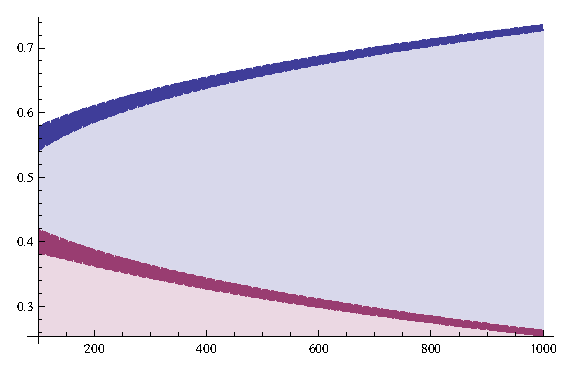
\includegraphics[width=0.6\textwidth]{figures/concorcetjury.eps}
  \caption{陪审团做出正确决定的概率}\label{fig:concorcetjury}
\end{figure}

孔多赛陪审团定理的不足之处在于其假设过于理想,比如陪审员或者投票人每个人的价值观念都不同,由于相互影响,可能更多的是以团体形式进行表决或投票,因此独立性假设与等概率假设就站不住脚;此外,在投票理论中,候选人不能通过简单的优化理论做出评价,从而难以选择出“最佳”候选人;当投票人不同、候选人得票率不同的情况下,利用简单的多数投票准则并不能得到满意的结果,即出现投票分割问题。

孔多塞方法是一类方法,我们下面介绍几个典型的孔多塞方法:柯普兰方法、凯梅尼─杨格方法、最小最大法、南森方法、道奇森方法、排名序方法和舒尔茨方法,并分析各自的性质。

\begin{definition}[孔多塞准则]
对于任意的$\mathcal A$及偏好集$\Pi[\mathcal A, \mathcal M]$,如果候选人$x\in \mathcal A$是一个孔多塞赢家,则$x$是$\mathcal F$在偏好集$\Pi[\mathcal A,\mathcal M]$上的社会选择,并且是唯一的社会选择,则称社会选择函数$\mathcal F$满足孔多塞准则或孔多塞赢家准则(Condorcet Winner Criterion,CWC)。
\end{definition}

\subsubsection{柯普兰方法}
柯普兰方法(Copeland method)是一种孔多塞方法,它利用某个候选人在和其他候选人一对一循环对决中胜出局数与落败局数之差,换而言之是其所击败的候选人数目减去将其击败的候选人数目,作为其投票分值,即
\begin{equation}\label{eq:copeland}
    V_x = \big|\{y\in \mathcal A\mid x\succ_\Pi^\mathcal{F'} y\}\big| - \big|\{y\in \mathcal A\mid y\succ_\Pi^\mathcal{F'} x\}\big|, \forall x\in \mathcal A,
\end{equation}
最终投票分值最高的候选人胜出,其中$\mathcal{F'}$表示多数投票法。根据柯普兰方法,例子\ref{eg:1980usny}中三名候选人的得分是$V_H=2$,$V_D=0$,$V_J=-2$。

柯普兰方法属于零和博弈(zero sum game):候选人Holtzman是孔多塞赢家,将其他两个候选人D'Amato和Javits悉数击败,而Javits则是孔多塞输家
(Condorcet loser),在与其他两名候选人对决时皆落败。根据柯普兰得分,孔多塞赢家Holtzman胜出,并且社会偏好为$H\succ D\succ J$。

\subsubsection{凯梅尼─杨格方法}
凯梅尼─杨格方法(Kemeny-Young method)~\cite{kemeny1959mathematics},也称凯梅尼规则、最大似然模型,也是一种基于成对比较的投票方法。KY方法考虑每个可能的偏好排名,根据社会偏好集$\Pi[n,m]$计算各个偏好排名的分值,分值最高的排名是社会选择偏好排名。KY方法将每个个体偏好排名拆解成所有可能序对偏好,利用社会偏好集确定含有对应序对偏好的票数,将对应序对偏好的票数加和即是某个个体偏好的得分。

\begin{definition}[排名分值]
对于候选集$\mathcal A$,可以生成n(n-1)种可能的偏好序对。对于某个排名$\pi\in \Pi$,有$\pi^{-1}(1)\succ \pi^{-1}(2)\succ\cdots \succ \pi^{-1}(n)$,可抽取出n(n-1)/2种序对偏好$\pi^{-1}(i)\succ \pi^{-1}(j)$,$1\le i<j \le n$。如果个体偏好排名$\sigma\in \Pi[n,m]$包含某个序对偏好,则为其投一票,遍历偏好集可算出每个序对偏好在社会偏好集上的得票
\begin{equation}
    V(x, y) = \sum\limits_{\sigma\in \Pi[n,m]} \ind(x\succ_\sigma y), \forall x, y\in \mathcal A,
\end{equation}
则排名$\pi$的分值等于其上所有可能的偏好序对的得票之和
\begin{equation}
    V_\pi = \sum\limits_{x\succ_\pi y} V(x,y) = \sum\limits_{x,y\in \mathcal A} \bigg[\ind(x\succ_\pi y) \sum\limits_{\sigma\in \Pi[n,m]} \ind(x\succ_\sigma y)\bigg].
\end{equation}
\end{definition}

\begin{definition}
凯梅尼─杨格方法是搜索$\Pi$选择出排名分值最大的偏好排名,即解如下形式的优化模型
\begin{equation}\label{eq:kemeny-youngmethod}
    \pi_\mathcal F = \argmax\limits_{\pi\in \Pi} V_\pi.
\end{equation}
最优排名$\pi_\mathcal F$中排名最高的候选人$\pi_\mathcal F^{-1}(1)\in \mathcal A$是社会偏好集$\Pi[n,m]$上的社会选择。
\end{definition}

\begin{theorem}\label{th:kemeny-young-borda}
凯梅尼─杨格方法等价于从$\Pi$搜索一个与社会偏好集$\Pi[n,m]$内所有个体偏好最近的偏好排名$\pi_\mathcal F$,以尽可能和所有选民的个人偏好保持一致。
\begin{equation}\label{eq:kemeny-young-borda}
    \pi_\mathcal F = \argmin\limits_{\pi\in \Pi} \sum\limits_{\sigma \in \Pi[n,m]} \tau(\pi,\sigma),
\end{equation}
其中,$\tau$表示肯德尔距离度量公式。
\end{theorem}

\begin{example}
根据例子\ref{eg:1980usny},我们可以构建序对偏好计票表与排名分值分布表\ref{tbl:preferencescore}。对于偏好排名$D\succ H\succ J$,其分值是$D\succ H$、$D\succ J$和$H\succ J$三个序对偏好分值之和$V_{D\succ H\succ J}$=\text{49+60+66=175}。根据偏好排名的分值可知社会选择是孔多塞赢家Holtzman,社会偏好排名是$H\succ D\succ J$,而排名分值最低的偏好排名是$J\succ D\succ H$,恰好是社会偏好排名的完全逆排列。为了验证定理\ref{th:kemeny-young-borda},我们计算所有偏好列表对的肯德尔距离以及每个个体偏好排名与社会偏好集$\Pi[n,m]$的肯德尔距离,如表\ref{tbl:preferencedistancematrix}所示,表的末行数据是根据公式\ref{eq:kemeny-young-borda}计算得到的肯德尔距离之和,其他行数据表示对应行偏好列表与列偏好列表之间的肯德尔距离。比如个体偏好$H\succ J\succ D$ 与$J\succ D\succ H$的肯德尔距离是2/3,而$J\succ D\succ H$与社会偏好集的肯德尔距离
\[
    \tau(J\succ D\succ H, \Pi[n,m]) = 2/3\times 22 + 1/3\times 23 + 1\times 15 + 2/3\times 29 + 0\times 4 + 1/3\times 7 = 177/3
\]
最大,而$H\succ D\succ J$与社会偏好集的肯德尔距离最小,式\ref{eq:kemeny-youngmethod}和\ref{eq:kemeny-young-borda}的等价性得到实例验证。
\begin{table}[ht]
    \centering
    \begin{minipage}[t]{0.33\linewidth}
    \centering
    \begin{tabular}{c|ccc}
      \hline
       & $D$ & $H$ & $J$\\
      \hline
      $D$ & -- & 49 & 60\\
      $H$ & 51 & -- & 66\\
      $J$ & 40 & 34 & -- \\
      \hline
    \end{tabular}
    \end{minipage}
    \begin{minipage}[t]{0.65\linewidth}
    \centering
    \begin{tabular}{c|c|c|c}
      \hline
      偏好排名 & 排名分值 & 偏好排名 & 排名分值\\
      \hline
      $D\succ H\succ J$ & 175 & $D\succ J\succ H$ & 143\\ %49+60+66,60+49+34
      \textbf{$H\succ D\succ J$} & \textbf{177} & $H\succ J\succ D$ & 157\\ %51+66+60,66+51+40
      $J\succ D\succ H$ & 123 & $J\succ H\succ D$ & 125\\ %40+34+49,40+34+51
      \hline
    \end{tabular}
    \end{minipage}
    \caption{序对偏好计票表(左)与偏好排名分值分布表(右)}
    \label{tbl:preferencescore}
    \vspace{0.2cm}
    \begin{minipage}[t]{0.98\linewidth}
    \centering
    \begin{tabular}{c|cccccc}
      \hline
      & \small{$D\succ H\succ J$} & \small{$D\succ J\succ H$} & \small{$H\succ D\succ J$} & \small{$H\succ J\succ D$} & \small{$J\succ D\succ H$} & \small{$J\succ H\succ D$}\\
      \hline
      \small{$D\succ H\succ J$} & 0 & 1/3 & 1/3 & 2/3 & 2/3 & 1\\
      \small{$D\succ J\succ H$} & 1/3 & 0 & 2/3 & 1 & 1/3 & 2/3\\
      \small{$H\succ D\succ J$} & 1/3 & 2/3 & 0 & 1/3 & 1 & 2/3\\
      \small{$H\succ J\succ D$} & 2/3 & 1 & 1/3 & 0 & 2/3 & 1/3\\
      \small{$J\succ D\succ H$} & 2/3 & 1/3 & 1 & 2/3 & 0 & 1/3\\
      \small{$J\succ H\succ D$} & 1 & 2/3 & 2/3 & 1/3 & 1/3 & 0\\
      \hline
      $\tau(\pi,\Pi[n,m])$ & 125/3 & 157/3 & \textbf{123/3} & 143/3 & 177/3 & 175/3\\
      \hline
    \end{tabular}
    \end{minipage}
    \caption{偏好排名肯德尔距离矩阵}
    \label{tbl:preferencedistancematrix}
\end{table}
\end{example}

KY方法是一个NP-Hard问题~\cite{bartholdi1989voting},需要遍历整个偏好排名空间$\Pi$,难以直接优化求解。可以证明,KY方法与其他几种方法之间存在紧密联系:它是孔多塞方法的最大似然估计~\cite{young1995optimal},并且还与波达计数法对赢家和输家持有完全一致的偏好~\cite{saari2000geometric}。

\section{位置筛选法}
\subsection{单记可让渡投票制}
\textbf{单记可让渡投票制}(single transferable voting,STV),肇始于19世纪50年代,由英国的Thomas Hare和丹麦的George Andrae发明,用以选出唯一的赢家。

1871年美国建筑师威廉·罗伯特·威尔William Robert Ware提出\textbf{排序复选制}(instant-runoff voting,IRV),也称\textbf{选择投票制}(alternative voting)或\textbf{偏好投票制}(preferential voting),1918年始澳大利亚众议院选举、2010年奥斯卡最佳影片的评选都采纳了IRV方法。IRV方法统计候选人的第一票数(first choice \textit{or} first preference),任何候选人只要第一票数超出半数则胜出,选举结束;否则,将第一票数最低的候选人剔除,所有含有此候选人的偏好列表也要做剔除处理,重新统计第一票数,依次类推,直至有候选人以超过半数胜出。显然,IRV是STV的一个特例。

\section{概率模型法}
\subsection{马洛斯模型}
\textbf{马洛斯模型}(Mallows Model)是一种基于距离的排名聚合方法,它利用排列空间$\Pi[n]$上定义的距离度量指标,比如肯德尔距离、斯皮尔曼距离等,确定排列空间上的概率分布。假设初始排列(location permutation)为$\sigma$,对任意的排列$\pi\in \Pi[n]$,马洛斯模型定义如下形式的概率分布
\begin{equation}\label{eq:mallowsmodel}%parametric location-spread model
    P(\pi|\sigma; c) = \frac{\exp\{-c\times d(\pi, \sigma)\}}{\sum\limits_{\pi' \in \Pi[n]} \exp\big\{-c \times d(\pi', \sigma)\big\}},
\end{equation}
其中参数$c>0$称作\textbf{离散因子}(disperse),用以控制排列空间上的距离权重。根据模型定义,构建排列空间上的概率分布需要遍历整个空间,其计算复杂度高达$\complex(n!)$,以致于无法实际应用。

\subsection{瑟斯顿模型与TrueSkill排名}%\subsection{XBox评分和TrueSkill排名}

\subsection{布雷德利─特里─卢斯模型}%Bradley–Terry–Luce

\subsection{普拉基特─卢斯模型}
\textbf{普拉基特─卢斯模型}(Plackett-Luce model,也称“卢斯模型”,简称PL模型)是一种分步排名方法,假设每个参与排名的对象都对应一个隐性分值$z$,利用隐性分值评估$\Pi[n]$的分布概率。如果决策者根据某种准则产生一个排列$\pi$,则对象$\pi^{-1}(i)$在排列$\pi$中排到第$i$位的概率$P_i$,依赖于其自身的评分$z_{\pi^{-1}(i)}$,以及其他所有排名在它下面的其他所有对象的评分之和$\sum\limits_{i\le k\le n} z_{\pi^{-1}(k)}$。PL模型对每个评分统一作单调变换,有如下形式的定义
\[
    P_i = \frac{\exp(z_{\pi^{-1}(i)})}{\sum\limits_{i\le k\le n} \exp(z_{\pi^{-1}(k)})}, 1\le i \le n.
\]
根据独立性假设,则由隐性评分列表生成排列$\pi$的概率为
\begin{equation}\label{eq:luce}
    P(\pi) = \prod\limits_{i=1}^n P_i = \prod\limits_{i=1}^n\frac{\exp(z_{\pi^{-1}(i)})}{\sum\limits_{i\le k\le n} \exp(z_{\pi^{-1}(k)})}.
\end{equation}

如果计算排列$\pi$的生成概率,只考虑位置靠前的对象评分信息,排名靠后的对象评分信息直接忽略掉,实际上对于概率评估影响甚微。比如,只考虑前$K$个位置上的对象评分信息,可以计算生成排列$\pi$的近似生成概率$P(\pi;K)$,则有定义
\begin{equation}\label{eq:luce-topk}
    P(\pi; K) = \prod\limits_{i=1}^K \frac{\exp(z_{\pi^{-1}(i)})}{\sum\limits_{i\le k\le n}\exp(z_{\pi^{-1}(k)})} \ge P(\pi),
\end{equation}
这个概率称作$n$个对象排列的\textbf{TopK概率}。当$K=n-1$时,由于$P_n = 1$,则有
\[
    P(\pi;n-1)=P(\pi;n)=P(\pi).
\]
当$K=1$时有
\begin{equation}\label{eq:luce-top1}
    P(\pi; 1) = \frac{\exp(z_{\pi^{-1}(i)})}{\sum\limits_{i\le k\le n}\exp(z_{\pi^{-1}(k)})}.
\end{equation}
如果记$n$个对象生成的所有排列集合为$\Pi[n]$,我们可以建立$P(\pi)$与$P(\pi,K)$二者之间的联系:
\begin{equation}\label{eq:luce-and-topk}
    P(\pi; K) = \sum\limits_{\sigma\in \Pi[n,K,\pi]} P(\sigma).
\end{equation}

\begin{example}
假设四个对象$\{1,2,3,4\}$存在隐性分值$Z=\{0.5, 0.8, 0.3, 0.1\}$,随机排列可以生成$4!=24$种可能的结果,如图\ref{fig:permprob-kendall}所示的多面体,每个定点对应一个排列,根据卢斯模型可以计算生成各个排列的概率。如表\ref{tbl:permuprob}所示,所有排列概率之和等于$1$,排列$\pi=\langle 1,2,3,4 \rangle$的概率$P(\pi)= 0.068102079$,排列$\pi=\langle 2,1,4,3 \rangle$的概率$P(\pi)=0.063594464$。如果根据隐性分值进行排名,可以得到最理想的排列$\pi=\langle 2,1,3,4 \rangle$,其概率最大$P(\pi)= 0.07767445$,对应图\ref{fig:permprob-kendall}中最大节点,最不理想的排列是$\pi=\langle 4,3,1,2\rangle$,其概率最小$P(\pi)=0.019200285$,对应图\ref{fig:permprob-kendall}中最小节点。

\begin{figure}[htbp]
  \centering
  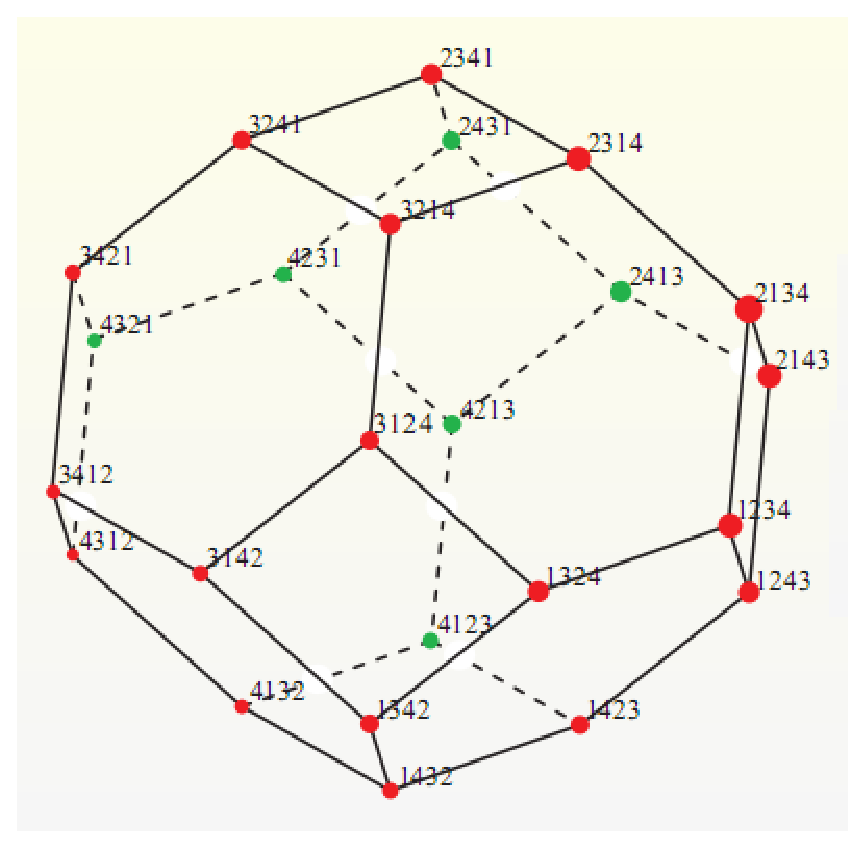
\includegraphics[width=0.5\textwidth, height=7cm]{figures/permprob-kendall.eps}\\
  \caption{排列分布及分布肯德尔距离,$1234 \triangleq \langle 1,2,3,4 \rangle$}\label{fig:permprob-kendall}
\end{figure}

\begin{table}[htbp]
    \centering
    \begin{tabular}{|c|c|c|c|c|c|c|}
\hline
$\pi$ & $\langle 1,2,3,4\rangle$ & $\langle 1,2,4,3\rangle$ & $\langle 1,3,2,4\rangle$ & $\langle 1,3,4,2\rangle$ & $\langle 1,4,2,3\rangle$ & $\langle 1,4,3,2\rangle$\\
$P(\pi)$ & 0.068102079 & 0.055757275 & 0.05019727 & 0.024927228 & 0.038285447 & 0.023221297\\
\hline
$\pi$ & $\langle2,1,3,4\rangle$ & $\langle2,1,4,3\rangle$ & $\langle2,3,1,4\rangle$ & $\langle2,3,4,1\rangle$ & $\langle2,4,1,3\rangle$ & $\langle2,4,3,1\rangle$\\
$P(\pi)$ & \bf{0.07767445} & 0.063594464 & 0.069244944 & 0.046416276 & 0.052066751 & 0.042628653\\
\hline
$\pi$ & $\langle3,1,2,4\rangle$ & $\langle3,1,4,2\rangle$ & $\langle3,2,1,4\rangle$ & $\langle3,2,4,1\rangle$ & $\langle3,4,1,2\rangle$ & $\langle3,4,2,1\rangle$\\
$P(\pi)$ & 0.047184467 & 0.023431114 & 0.057067546 & 0.038253525 & 0.020143783 & 0.027191263\\
\hline
$\pi$ & $\langle4,1,2,3\rangle$ & $\langle4,1,3,2\rangle$ & $\langle4,2,1,3\rangle$ & $\langle4,2,3,1\rangle$ & $\langle4,3,1,2\rangle$ & $\langle4,3,2,1\rangle$\\
$P(\pi)$ & 0.03430199 & 0.020805209 & 0.040900468 & 0.033486473 & \bf{0.019200285} & 0.025917675\\
      \hline
    \end{tabular}
    \caption{排列分布表}
    \label{tbl:permuprob}
\end{table}

根据定义,Top-2的排列分布(表\ref{tbl:permuprob-top1-2})可通过Top-3的排列分布计算,比如$\langle 1,2,*,*\rangle$的概率等于$\langle 1,2,3,4\rangle$ 与$\langle 1,2,4,3\rangle$ 的概率之和,即有
\[
\begin{array}{lcl}
    P(\langle 1,2,3,4\rangle) + P(\langle 1,2,4,3\rangle) & = &  0.068102079 + 0.055757275\\
    & = & P(\langle 1,2,*,*\rangle) = 0.123859355.
\end{array}
\]
Top-1排列分布(表\ref{tbl:permuprob-top1-2})可以通过Top-2的排列分布进行计算,如$\langle 3,*,*,*\rangle$的概率又等于$\langle 3,1,*,*\rangle$、$\langle 3,2,*,*\rangle$和$\langle 3,4,*,*\rangle$ 的概率之和,即有
\[
\begin{array}{lcl}
    P(\langle 3,1,*,*\rangle) + P(\langle 3,2,*,*\rangle) + P(\langle 3,4,*,*\rangle)& = & 0.070615583 + 0.095321069 + 0.047335044 \\
    & = & P(\langle 3,*,*,*\rangle) = 0.2133.
\end{array}
\]

\begin{table}[htbp]
    \centering
    \begin{tabular}{|c|c|c|c|c|c|c|}
      \hline
       $\pi; 2$ & $\langle 1,2,*,*\rangle$ & $\langle 1,3,*,*\rangle$ & $\langle 1,4,*,*\rangle$ & $\pi;1$ & $\langle 1,*,*,*\rangle$\\
       $P(\pi; 2)$ & 0.123859355 & 0.075124501 & 0.061506748 & $P(\pi; 1)$ & 0.2605\\
      \hline
       $\pi; 2$ & $\langle 2,1,*,*\rangle$ & $\langle 2,3,*,*\rangle$ & $\langle 2,4,*,*\rangle$ & $\pi;1$ & $\langle 2,*,*,*\rangle$\\
       $P(\pi; 2)$ & 0.141268922 & 0.11566122 & 0.094695399 & $P(\pi; 1)$ & 0.3516\\
      \hline
       $\pi; 2$ & $\langle 3,1,*,*\rangle$ & $\langle 3,2,*,*\rangle$ & $\langle 3,4,*,*\rangle$ & $\pi;1$ & $\langle 3,*,*,*\rangle$\\
       $P(\pi; 2)$ & 0.070615583 & 0.095321069 & 0.047335044 & $P(\pi; 1)$ & 0.2133\\
      \hline
       $\pi; 2$ & $\langle 4,1,*,*\rangle$ & $\langle 4,2,*,*\rangle$ & $\langle 4,3,*,*\rangle$ & $\pi;1$ & $\langle 4,*,*,*\rangle$\\
       $P(\pi; 2)$ & 0.055107202 & 0.074386937 & 0.045117957 & $P(\pi; 1)$ & 0.1746\\
      \hline
    \end{tabular}
    \caption{Top-2与Top-1排列分布表}
    \label{tbl:permuprob-top1-2}
\end{table}
\end{example}

\subsection{Elo排序系统}
\subsection{Colley方法}
\subsection{Massey方法}

由于地理、文化等社会人文环境的差异,世界范围内已经诞生数量可观的社会选择方法。为了分析各种方法,便于对其区分和归类,人们提出一系列性质良好的投票系统准则,如多数准则(majority criterion)、孔多塞一致性准则(Condorcet consistency)等单赢家投票系统准则。我们使用一个小节专门来介绍它们。

\section{投票系统准则}
\begin{definition}[多数准则]
如果半数以上的选民选择(或偏好)某个候选人,则此人一定是社会选择。
\end{definition}

\begin{corollary}
孔多塞方法、IRV方法、Bucklin方法和多数投票方法都满足多数准则。
\end{corollary}

\begin{definition}[孔多塞准则]
如果存在一个候选人,在和其他候选人的一对一循环对决中总能胜出,则此候选人必然胜出。
\end{definition}

\begin{corollary}
如果一个单赢家投票系统满足孔多塞准则,则它必然也满足多数准则。
\end{corollary}

\begin{corollary}
布莱克方法、柯普兰方法、道奇森方法、凯梅尼─杨格方法、最小最大法、南森方法、有序对方法(ranked pairs)和舒尔茨方法都满足孔多塞准则。
\end{corollary}

\begin{definition}[一致性准则]
假设将社会偏好集$\Pi[n,m]$任意分割成两个或多个子集,使得某个候选人$x\in \mathcal A$是每个社会偏好子集上的社会选择,如果$x$也是$\Pi[n,m]$上的社会选择,则称对应社会选择函数满足一致性准则(consistency criterion)或可分性准则(separability criterion)。
\end{definition}

\begin{corollary}
如果一个排序投票系统(ranked voting system)满足一致性,当且仅当它也是一个位置投票系统(positional voting system)。波达方法满足一致性,但柯普兰方法、IRV方法、凯梅尼─杨格方法、最小最大法、有序对方法(ranked pairs)和舒尔茨方法都违反一致性准则。
\end{corollary}

\begin{definition}[排名一致性准则]
假设将社会偏好集$\Pi[n,m]$任意分割成两个或多个子集,使得某个排序$\pi\in \Pi[n]$是每个社会偏好子集上的社会选择排序,如果$\pi$也是$\Pi[n,m]$上的社会选择排序,则称对应社会选择函数满足排名一致性准则(ranking consistency criterion)。
\end{definition}

\begin{corollary}
凯梅尼─杨格方法满足排名一致性准则。
\end{corollary}

\section{阿罗不可能定理}
1951年,美国经济学家肯尼斯·阿罗Kenneth Arrow~\cite{arrow1950difficulty,arrow2012social}使用数学公理化的方法研究社会决策时,证明了一个重要的结论:如果众多的社会成员具有不同的偏好,而社会又有多种备选方案,那么在民主的制度下不可能得到令所有的人都满意的结果。换句话说,依靠简单的“少数服从多数”的投票原则,在各种个人偏好中选择出一个共同一致的顺序,无法实现。简而言之,阿罗证明“完美的投票体系是不存在的”,即声名远播的\textbf{阿罗不可能定理}(Arrow's Impossibility Theorem)或\textbf{阿罗悖论}(Arrow's Paradox)。阿罗悖论不啻于一声惊雷,对当时的政治哲学和福利经济学产生了巨大的冲击,并为阿罗摘得1972年的诺贝尔经济学奖。

%英国哲学家约翰·洛克John Locke认为“根据自然和理性的法则,大多数具有全体的权力,因而大多数的行为被认为是全体的行为,也当然有决定权了”。在现代社会,多数原则(Majority Principle)已然成为广泛认可的社会决策方法。

社会选择,在数学上表示一个建立在所有个体偏好上的函数(或映射),其性质反映了一定的价值规范,如公民权、帕累托有效、无独裁性等。社会选择最重要的问题是:能否从逻辑上协调所有这些价值规范。阿罗使用公理性的证明,向人们宣告一个不幸的消息:世上没有同时满足\textbf{个人偏好的无限制性}、\textbf{帕累托有效}
\footnote{帕累托Vilfredo Pareto(1848~1923),意大利经济学家和社会学家。曾在都灵大学就读,后在意大利一家大型铁路公司担任工程师,升至主管,1893年起任瑞士洛桑大学教授。在经济学和社会学两个领域做出突出贡献,1906年提出帕累托最优状态(Pareto optimal)的概念,也成帕累托有效性(Pareto efficiency),奠定了现代福利经济学的基础。他认为,只要有可能使至少一个人更富裕,而同时又能使其他人保持在原来的生活水平,社会资源分配就没有达到最佳状态。}、\textbf{非相关目标独立性}与\textbf{非独裁性}四个基本公理的社会选择函数。

\begin{definition}[个人偏好的无限制性]
如果社会选择函数$\mathcal F$允许所有逻辑上可能存在的个人偏好自由表达,则称其满足无限制性(unrestricted domain)或完整性
(universality)。
\end{definition}

\begin{definition}[帕累托有效性]
对任意$x,y\in \mathcal A$,如果所有决策者一致认定$x\succ y$,则社会偏好列表$\pi_\mathcal F$也有$x\succ y$,即$x\succ_{\Pi[n,m]}^{\mathcal F} y$,则称社会选择函数$\mathcal F$满足帕累托有效性(Pareto efficiency),也称一致同意性(unanimity)。
\end{definition}

\begin{definition}[非相关目标独立性]
对于两个社会偏好集$\Pi[n,m]=\{\pi_i\}_{i=1}^m$与$\Pi'[n,m]=\{\pi'_i\}_{i=1}^m$,$\pi_i$与$\pi'_i$对应同一个决策者,$1\le i \le m$。如果每个决策者关于$x,y\in \mathcal A$的个人偏好保持不变:
\begin{equation}
    x\succ_{\pi_i} y \Leftrightarrow x\succ_{\pi'_i} y,~~1\le i\le m,
\end{equation}
则集体关于$x,y$的社会偏好在两个社会偏好集$\Pi[n,m]$和$\Pi'[n,m]$上也不会发生变化:
\begin{equation}
    x\succ_{\Pi[n,m]}^{\mathcal F} y\Leftrightarrow x\succ_{\Pi'[n,m]}^{\mathcal F} y,
\end{equation}
此时称社会选择函数$\mathcal F$满足非相关目标独立性(Independence of Irrelevant Alternatives,IIA)。
\end{definition}

\begin{definition}[非独裁性]
对于一个决策者,如果社会选择$\mathcal F$完全等价于其个人偏好$\pi$,即
\begin{equation}
    x\succ_\pi y\Leftrightarrow x\succ_{\Pi}^{\mathcal F} y,
\end{equation}
则称其为独裁者(dictator)。如果集合$\mathcal M$中没有独裁者,则称社会选择函数$\mathcal F$满足非独裁性(non-dictatorship)。
\end{definition}

\begin{definition}[线性序]
非空集合$\mathcal A$上的二元关系$\succ$称作是\textbf{线性序}(linear ordering),如果它满足
\begin{itemize}
    \item 反对称性(anti-symmetric):对任意的$x,y\in \mathcal A$,只要$x\succ y,~y\succ x$,都有$x=y$,
    \item 传递性(transitive):对任意的$x,y,z\in \mathcal A$,只要$x\succ y,~y\succ z$,都有$x\succ z$,
    \item 完备性(complete):对任意的$x,y\in \mathcal A$,要么$x\succ y$,要么$y\succ x$。
\end{itemize}
\end{definition}

\begin{definition}[社会福利函数]
如果社会选择函数$\mathcal F: \Pi[n,m]\mapsto \Pi[n]$是$\mathcal A$上的一个线性序,则称其为线性投票规则或社会福利函数(social welfare function),而其完备性对应于个人偏好的无限制性。
\end{definition}

\begin{theorem}[阿罗不可能性定理]
如果$|\mathcal A|=n>2$,则兼具帕累托有效性、非独裁性和IIA的线性投票规则$\mathcal F$不存在。换言之,兼具帕累托有效性和IIA的线性投票规则一定存在独裁者。
\end{theorem}

我们下面详细介绍1998年诺贝尔经济学奖得主阿马蒂亚·森Amartya Sen
\footnote{阿马蒂亚·森1933年生于英属印度西孟加拉邦桑蒂克尼盖登,1953年获加尔各答大学文学学士学位,1955年前往剑桥大学攻读第二个学士学位,并于1959年在剑桥大学获得博士学位。1971年起在伦敦经济学院任教,1977年起任牛津大学经济学教授,70年代末转教于美国哈佛大学。1998年1月又返回英国剑桥大学,担任三一学院
(Trinity College,Cambridge)院长。他克服了阿罗不可能定理衍生的难题,对福利经济学基础理论做出巨大贡献。}对阿罗不可能性定理的证明思路,为此先引入决定性联盟(decisive coalition)的概念。

\begin{definition}[决定性联盟]
对于非空集合$\mathcal M_c\subset \mathcal M$,以及$x,y\in \mathcal A$,如果满足
\begin{equation}
    x\succ_{\Pi[\mathcal A, \mathcal M_c]}^{\mathcal F} y \Leftrightarrow x\succ_{\Pi[\mathcal A, \mathcal M]}^{\mathcal F} y,
\end{equation}
则称$\mathcal M_c$是决定社会选择$\mathcal F$关于$(x,y)$偏好的决定性联盟。如果对任意$x,y\in \mathcal A$,$\mathcal M_c$都是决定$\mathcal F$关于$(x,y)$偏好的决定性联盟,则称$\mathcal M_c$是$\mathcal F$的决定性联盟。如果$\mathcal M_c$是所有偏好$x$甚于$y$的决策者集合,
\end{definition}
决定性联盟可以操控社会选择,严重侵害其他社会成员的利益。如果$|\mathcal M_c|>1$,决定性联盟构成寡头,在寡头集团操控下的政治生态形成寡头政治。如果$|\mathcal M_c|=1$,决定性联盟就是独裁者。我们可以证明:如果$\mathcal F$满足帕累托有效性,则$\mathcal M$是$\mathcal F$的决定性联盟。森巧妙地利用决定性联盟,推导出阿罗不可能性定理:兼具个人偏好无限制性、帕累托有效性和IIA的线性投票规则由单点集决定性联盟所操纵,即存在独裁者。

\begin{definition}[弱决定性联盟]
给定投票规则$\mathcal F$,称非空集$G\subseteq \mathcal N$是$\mathcal F$对$(x,y)$的弱决定性联盟,若对任意排序组合$\pi$,只要$G$中的成员恰好是$x\succ y$ 的所有赞成者,则社会排序$\mathcal F(\pi)$中也有$x\succ y$,即$x\succ_\pi^{\mathcal F}y$。
\end{definition}
若$G$是$\mathcal F$对$(x,y)$的决定性联盟,则$G$也是$\mathcal F$对$(x,y)$的弱决定性联盟。反过来是否成立呢?如果$\mathcal F$满足帕累托条件和独立性条件,则反过来不仅成立,而且我们还有如下更强的结论:
\begin{lemma}
设$\mathcal{F}$是满足帕累托条件和独立性条件的线性投票规则。若$G$是$\mathcal F$对$(x,y)$的弱决定性联盟,则$G$是$\mathcal F$的决定性联盟,即$G$是$\mathcal F$对任意$(x',y')$的决定性联盟。
\end{lemma}
\begin{proof}
设$\mathcal{F}$是满足帕累托条件和独立性条件的线性投票规则。设$G$是$\mathcal F$对$(x,y)$的弱决定性联盟,任给$(x',y')$,我们证明$G$是$\mathcal F$对任意$(x',y')$的决定性联盟。不妨设$x',y'$与$x,y$均不相同(相同的情况类似可证)。任给排序组合$\pi$,使得$G$中所有成员一致认为$x'\succ y'$,只需证$x'\succ_\pi^{\mathcal F}y'$。考虑如下的排序组合$\pi'$,其中
\begin{itemize}
  \item $G$中的投票者认为:$x'\succ_\pi^{\mathcal F}y'$;
  \item $G$之外的投票者认为:$x'\succ x$,$y\succ y'$,$y\succ x$,且对$x',y'$的排序与$\pi$保持一致。
\end{itemize}
易见,$G$中中的成员恰好是$x\succ y$的所有赞成者,由于$G$是$\mathcal F$对$(x,y)$的弱决定性联盟,故$x\succ_{\pi'}^{\mathcal F}y$。由于在$\pi'$中所有人都认为$x'\succ x$且$y\succ y'$,据帕累托条件有,$x'\succ_{\pi'}^{\mathcal F}x$且$y\succ_{\pi'}^{\mathcal F}y'$,据社会排序的传递性可得,$x'\succ_{\pi'}^{\mathcal F}y'$。注意到$\pi$与$\pi'$关于$x',y'$的排序上是一样的,由独立性条件有,$x'\succ_{\pi}^{\mathcal F}y'$,证毕。现在我们可以证明下面的收缩引理了。
\end{proof}

\begin{lemma}[收缩引理]
设$\mathcal F$是满足帕累托条件和独立性条件的线性投票规则。若非单点集$G$是$\mathcal F$的决定性联盟,则$G$的某个真子集$G'$也是$\mathcal F$的决定性联盟。
\end{lemma}
\begin{proof}
由于$G$是非单点集,故可将$G$拆分成两个不相交的非空子集$G_1$和$G_2$。考虑满足如下条件的排序组合$\pi$(由于备选项超过两个,故可以做到):
\begin{itemize}
  \item $G_1$中的投票者认为:$x\succ y\succ z$;
  \item $G_2$中的投票者认为:$y\succ z\succ x$;
  \item $G$之外的投票者(如果有的话)认为:$z\succ x\succ y$。
\end{itemize}
注意到$G$中所有投票者都认为$y\succ z$,由$G$是$\mathcal F$的决定性联盟可得,$y\succ_\pi^{\mathcal F} z$。现在分别考虑两种情况(由于$\mathcal F(\pi)$是完全的,故有且仅有两种情况):
\begin{itemize}
  \item $x\succ_\pi^{\mathcal F}z$。任给排序组合$\pi'$,使得$G_1$中的成员在$\pi'$中恰好是$x\succ z$的所有赞成者,由于在$\pi$中$G_1$中的成员也恰好是 $x\succ z$的所有赞成者,故由独立性条件可得,$x\succ_{\pi'}^{\mathcal F} z$,这意味着$G_1$是$\mathcal F$对$(x,z)$的弱决定性联盟,再据引理1有,$G_1$是$\mathcal F$的决定性联盟。
  \item $z\succ_\pi^{\mathcal F}x$。此时,据$\mathcal F(\pi)$的传递性有$y\succ_\pi^{\mathcal F}x$。同理于情况1可证,$G_2$是$\mathcal F$的决定性联盟。
\end{itemize}
综上,总有$G$的真子集是决定性联盟,证毕\footnote{Logic:\href{http://www.cnblogs.com/ilogic/archive/2012/08/05/proof\_arrow.html}{阿罗不可能性定理的证明}}。
\end{proof}

\section{吉伯德-萨特思韦特定理}
19世纪80年代,投票选举理论的奠基人之一查尔斯·勒特威奇·道奇森Charles Lutwidge Dodgson
\footnote{查尔斯·勒特威奇·道奇森(1832--1898),笔名路易斯·卡罗尔Luis Carroll,英国数学家、《艾丽丝漫游奇境记》及续篇《爱丽丝镜中奇遇》的作者。他天赋异禀,在几何学、线性代数、矩阵与逻辑学面都颇有研究,写出十多本数学著作,为线性代数与概率论两大领域提供了新思路。他认为一个合理的选举规则应当在孔多赛赢家存在时始终选择孔多赛赢家,在孔多赛赢家不存在时,仍然能够选择最接近于孔多赛赢家的候选人:(孔多赛赢家不存在),他的这一思想被人称作道奇森准则。}
开始关注对投票规则的研究,认为人们在投票时的行为更倾向于策略投票。个人出于某种目的策略性的需要,通过谎报自己的真实偏好,使得决策结果往有利的方向变化。个人谎报其真实偏好,可能会造成损人不利己的后果,选出对各方均不利的候选人,对公众权利产生不利影响。为此有必要深入研究策略性投票对选举的操纵,以期设计出防止策略性投票的社会选择方法。

如果在投票选举时存在策略性投票,个人所表达的偏好偏离其真实偏好,研究学者有理由重新审视阿罗不可能定理。20世纪70年代密歇根大学的阿兰·吉伯德Allan Gibbard 和西北大学的马克·萨特思韦特Mark Satterthwaite分别独立提出两个几乎相同的定理,统称\textbf{吉伯德-萨特思韦特定理}(Gibbard--Satterthwaite Theorem)防策略投票的不可能性定理,引起数学、经济学、计算机科学和哲学等诸多领域学者的广泛关注。

\begin{definition}[战略免疫性]
如果其他个体均真实披露自己偏好信息,某个特定个体只有真实显示自己的偏好时社会选择对自己才最有利,则称对应社会选择规则可免于战略性投票操纵
(non-manipulable),即具有\textbf{战略免疫性}(strategy-proofness)。
\end{definition}

\begin{theorem}[吉伯德-萨特思韦特定理]
在社会选择规则集合内不存在同时满足个人偏好无限制性、帕累托有效性、非独裁性、传递性和战略免疫性五个基本公理的选择规则。
\end{theorem}
根据吉伯德─萨特思韦特定理,我们意识到非独裁性和战略免疫性两个属性可能存在内在矛盾,任何合理的社会选择规则都难以两面兼顾:在所有可能的社会选择规则下,能够同时满足个人偏好无限制性、帕累托有效性、传递性和战略免疫性的只有独裁规则。如果存在一个社会选择规则兼具个人偏好无限制性、帕累托有效性、非独裁性和传递性,则它必定无法免于战略性投票操纵。

许多社会选择方法满足一系列良好的公理性质,但是却免不了受到战略性投票的操控,总是存在隐瞒自己真实偏好的个体,试图取得对自己有利的选举局面。人们无法设计出一个确保或诱使所有个体能够道出其真实偏好(revelation principle)的社会选择机制。人们只能另辟蹊径,将目光转移到社会选择战略性操纵复杂度的研究,通过增加战略性投票操纵的成本,以降低人们投出违心选票的动机,比如20世纪90年代乔治亚理工学院教授约翰·巴托尔迪三世John Bartholdi III等人\cite{bartholdi1989computational,bartholdi1989voting}的卓越工作,促进了计算社会选择的快速发展:以高计算复杂度阻止策略性投票操纵,间接地迫使个体对其偏好做出真实的回应。由于选举操纵能够抑制部分个体耍诈,已然成为衡量一个社会选择准则优劣性的一个指标。

\section{梅定理}
\begin{definition}[匿名性]
如果集体选择的结果只依赖于各个个体的偏好与决策,与特定决策由具体谁做出无关,则称此集体选择具备\textbf{匿名性}(anonymity),或称决策者是对称主体。
\end{definition}

\begin{definition}[中立性]
如果决策规则在任意两个备选对象之间中立,则称它满足\textbf{中立性}(neutrality)。对于线性序形式的偏好排名,对于$m$个备选对象,存在$m!$种偏好排名,如果决策者的数目是$n$,则所有决策者可能产生的偏好排名组合有$m!^n$个。对于任意一个排名排名组合$P$,决策规则$r$的选择$r(P)=c$,对所有偏好排名组合$P$所含的所有偏好排名施加相同的排列运算$M$,如果决策规则选择$r(M(P))=M(r(P))$,则称它满足中立性。
\end{definition}

\begin{definition}[正向响应]
正向响应(positively responsive)
\end{definition}

\begin{theorem}[梅定理May's Theorem]
在集体选择的备选对象是二元的情况下,一种集体决策规则是简单多数规则,当且仅当它满足匿名性、中立性和正向响应。
\end{theorem}

%\section{Manipulations of Voting}

\section{排名聚合}
\textbf{排名聚合}(rank aggregation),也称\textbf{数据融合}(data fusion),源于投票选举问题,通过融合多个来源的对象排名结果,从而更加准确地反映对象间的优先等级秩序。目前,排名聚合已经在网络信息检索、统计检验、体育竞技排名等多个领域得到广泛应用,比如元搜索引擎接收用户提交的检索词,同时向多个基本搜索引擎的发送检索请求,将多个基本搜索引擎的搜索结果聚合而形成最终结果反馈给用户。

排名聚合的目标是从$\Pi[n]$中搜索一个理想的排列$\hat\pi$,使得它和所有已知排名列表$\{\pi_1,\pi_2,\ldots\}$保持尽可能的一致,数学上等价于解一个优化问题:
\begin{equation}\label{eq:rankaggregationproblem}
    \hat\pi = \argmax\limits_{\pi\in \Pi[n]} \sum\limits_i s(\pi,\pi_i) = \argmin\limits_{\pi\in \Pi[n]} \sum\limits_i d(\pi,\pi_i),
\end{equation}
其中$s(\pi,\sigma)$是衡量两个排名列表$\pi$和$\sigma$之间的相似性指标,$d(\pi,\sigma)$是由相似性指标$s(\pi,\sigma)$导出的某种距离度量,如肯德尔Tau。

\begin{table}[htbp]
\centering
\begin{tabular}{|c|l|c|l|}
\hline
编号 & 网址 & 编号 & 网址\\
\hline
1 & abcnews.go.com/health & 8 & www.cnn.com/HEALTH\\
2 & en.wikipedia.org/wiki/Health & 9 & www.health.com\\
3 & en.wikipedia.org/wiki/Health\_care & 10 & www.mayoclinic.com\\
4 & health.yahoo.net & 11 & www.nytimes.com/pages/health/\\
5 & health.gov & 12 & www.pacificprime.com\\
6 & reuters.com/news/health & 13 & www.webmd.com\\
7 & wiki.ask.com/Health &&\\
\hline
\end{tabular}
\caption{九个搜索引擎检索关键词“health”的十三条搜索结果}
\label{tbl:metaserp}
\end{table}

\begin{table}[htbp]
\centering
\begin{tabular}{|l|c|l|c|l|c|}
\hline
搜索引擎 & 搜索结果 & 搜索引擎 & 搜索结果 & 搜索引擎 & 搜索结果\\
\hline
AOL & $\langle 9,13,10,2,8\rangle$ & Bing & $\langle 2,13,4,5,11\rangle$ & DuckDuckGo & $\langle 4,13,2,1,6\rangle$ \\
Excite & $\langle 13,2,11,4,8\rangle$ & Google & $\langle 2,3,9,4,12\rangle$ & HotBot & $\langle 2,13,4,8,10\rangle$ \\
Lycos & $\langle 2,13,4,8,10\rangle$ & Teoma & $\langle 9,13,10,7,8\rangle$ & Yahoo! & $\langle 13,2,4,8,10\rangle$\\
\hline
\end{tabular}
\caption{九个搜索引擎检索关键词“health”的前5条搜索结果}
\label{tbl:serplist}
\end{table}

\begin{example}\label{eg:metasearch}
人们在使用搜索引擎检索信息时,比如提交检索词“health”,不同搜索引擎搜索并返回的结果通常也不相同。目前,正常提供服务的搜索引擎不下于1,000个。2011年10 月22 日,我们使用9个搜索引擎:
\underline{A}OL、\underline{B}ing、\underline{D}uckDuckGo、\underline{E}xcite、\underline{G}oogle、\underline{H}otBot、\underline{L}ycos、
\underline{T}eoma和\underline{Y}ahoo!,分别检索关键词“Health”,提取每个搜索引擎的前5条搜索条目汇集成13条搜索结果,如表\ref{tbl:metaserp}所示根据字母顺序为搜索条目对应网址编号,表\ref{tbl:serplist}是每个搜索引擎前5条搜索条目的排列结果。根据波达计数法则对搜索条目进行评分,如表\ref{tbl:bordarank}所示,第2 列至第14列是各个搜索引擎在对应搜索条目上的评分,聚合排名的结果是
\[
    \pi = \langle 13,2,4,8,10,9,11,3,1/5/7,6/12\rangle,
\]
其中$a/b$表示$a$和$b$评分相同,无法区分。如果我们预先对各个搜索引擎设定一个权值,比如
\[
\begin{array}{lcccccccccl}
    \omega &= &\{\omega_A,& \omega_B, & \omega_D & \omega_E, & \omega_G, & \omega_H, & \omega_L,&\omega_T, & \omega_Y\} \\
    &= & \{0.80, & 0.98, & 0.80, & 0.80, & 1.00, & 0.85, & 0.85, & 0.88, & 0.95\},
\end{array}
\]
重新计算加权评分,则有聚合排名结果
\[
    \pi_\omega = \langle 2,13,4,8,10,9,11,3,5,12,7,1,6\rangle.
\]
\end{example}
\begin{table}[htbp]
\centering
\begin{tabular}{|l|c|c|c|c|c|c|c|c|c|c|c|c|c|}
\hline
Rank & 1 & 2 & 3 & 4 & 5 & 6 & 7 & 8 & 9 & 10 & 11 & 12 & 13\\
\hline
A (0.80) &  & 10 &  &  &  &  &  & 9 & 13 & 11 &  &  & 12\\
B (0.98) &  & 13 &  & 11 & 10 &  &  &  &  &  & 9 &  & 12\\
D (0.80) & 10 & 11 &  & 13 &  & 9 &  &  &  &  &  &  & 12\\
E (0.80) &  & 12 &  & 10 &  &  &  & 9 &  &  & 11 &  & 13\\
G (1.00) &  & 13 & 12 & 10 &  &  &  &  & 11 &  &  & 9 &  \\
H (0.85) &  & 13 &  & 11 &  &  &  & 10 &  & 9 &  &  & 12\\
L (0.85) &  & 13 &  & 11 &  &  &  & 10 &  & 9 &  &  & 12\\
T (0.88) &  &  &  &  &  &  & 10 & 9 & 13 & 11 &  &  & 12\\
Y (0.95) &  & 12 &  & 11 &  &  &  & 10 &  & 9 &  &  & 13 \\
\hline
TS & 10 & 97 & 12 & 77 & 10 & 9 & 10 & 57 & 37 & 49 & 20 & 9 & 98\\
\hline
WTS & 8.0 & 85.64 & 12.0 & 68.33 & 9.8 & 7.2 & 8.8 & 48.82 & 32.84 & 42.33 & 17.62 & 9.0 & 84.67\\
\hline
\end{tabular}
\caption{波达排名与加权波达排名列表:首列括号内数值是各搜索引擎的权值,TS是各条目的总得分(Total Score),WTS是各条目的加权总得分
(Weighted Total Score)。}
\label{tbl:bordarank}
\end{table}

\subsection{序对投票准则}
设有$n$个候选人$\{1,2,\ldots,n\}$,每个选民都从中选出部分候选人并排列,所有选民的排列集合记作$\Pi$。每个排列$\pi\in \Pi$反映一个选民对部分候选人的偏好,越是其喜欢的候选人在选票中的排名越靠前。我们提出一种\textbf{序对投票}(pairwise voting, PV)准则,根据所有候选人组合在$\pi$ 中的相对名次进行评分。PV准则对所有没有入选$\pi$的候选人等同视之,则有$\pi(i)=|\pi| + 1$。对于某个候选人组合$(i,j)$,我们根据如下形式的序对投票准则构建序对评分矩阵$V(\pi)\in \mathbb R^{n\times n}$:
\begin{equation}\label{eq:pvc}
    v_\pi(i,j) = \frac{\pi(j)-\pi(i)}{\min\{\pi(i),\pi(j)\}}.
\end{equation}
当$\pi(i) < \pi(j)$时,候选人$i$在$\pi$中的排名比$j$的排名靠前,则$v_\pi(i,j)>0$;当$\pi(i) > \pi(j)$时,候选人$i$在$\pi$中的排名比$j$的排名靠后,则$v_\pi(i,j)=-v_\pi(j,i) < 0$;当$v_\pi(i,j)=v_\pi(j,i)$时,则$v_\pi(i,j)=0$。由此可知,序对评分矩阵$V(\pi)$是一个反对称矩阵$V(\pi) = -V^T(\pi)$。

每个候选人对应评分矩阵$V$的一行,如果计算序对评分矩阵的行和,则可以直接确定候选人从单个选民排名列表中的综合得分。实际上,评分矩阵每个行元可以看作是一次比赛结果。如果比赛胜利,则得分为正,比赛失利则得分为负。对于任意一个候选人$i$,它从某个选民排名列表$\pi\in \Pi$获得的总分记作$V_i(\pi)$,则有
\begin{equation}
    V_i(\pi) = \sum\limits_{1\le j\le n} v_\pi(i,j) = \sum\limits_{1\le j\le n} \frac{\pi(j)-\pi(i)}{\min\{\pi(i),\pi(j)\}}.% = -[(i-1) + \frac{i-2}{2} + \ldots + \frac{1}{i-1}] + \frac{1 + \ldots + (m - i)}{i}+ (n - m) \frac{m - i + 1}{i},
\end{equation}

如果记$\mathscr P_{i*}(\pi)=\{1\le j\le n, \pi(i) < \pi(j)\}$,$\mathscr P_{*i}(\pi)=\{1\le j\le n, \pi(j) < \pi(i)\}$分别对应$\pi$中排到候选人$i$之后的候选人集合、排到候选人$i$之前的候选人集合,利用它改写上式,则有
\begin{equation}
\begin{array}{lcl}
    V_i(\pi) &=& \sum\limits_{1\le j\le n} \frac{\pi(j)-\pi(i)}{\min\{\pi(i),\pi(j)\}} =  \sum\limits_{j\in \mathscr P_{i*}(\pi)} \frac{\pi(j)-\pi(i)}{\pi(i)} + \sum\limits_{j\in \mathscr P_{*i}(\pi)} \frac{\pi(j)-\pi(i)}{\pi(j)}\\
    &=& \sum\limits_{j\in \mathscr P_{i*}(\pi)} \big[\frac{\pi(j)}{\pi(i)} -1\big] + \sum\limits_{j\in \mathscr P_{*i}(\pi)} \big[1-\frac{\pi(i)}{\pi(j)}\big],\\
    &=& \sum\limits_{\pi(i)+1\le k \le |\pi|} \big[\frac{k}{\pi(i)} -1\big] + [n-|\pi|][\frac{|\pi|+1}{\pi(i)}-1] + \sum\limits_{1\le k \le \pi(i)-1} \big[1-\frac{\pi(i)}{k}\big].
\end{array}
\end{equation}
可以证明:$V_i(\pi)$是一个关于$\pi(i)$单调不增函数。当候选人落选$\pi$,$\pi(i)=|\pi|+1$,前两部分都等于零,则有
\begin{equation}
    V_i(\pi) = |\pi| - \pi(i)\sum\limits_{1\le k \le |\pi|} \frac{1}{k}.
\end{equation}
对于排在首位的候选人$i$,$\pi(i)=1$,其分值$V_1(\pi)=m(2n-m-1)/2$。

我们根据PV准则确定每个选民排名列表产生的评分矩阵,通过行和运算获得每个候选人在各个排名列表$\pi$所得综合评分。如果累积候选人在所有选民排列上的综合评分,从而可以算得其最终投票得分
\begin{equation}\label{eq:pvagg}
    V_i = \sum\limits_{\pi\in\Pi} V_i(\pi) = \sum\limits_{\pi\in\Pi} \sum\limits_{1\le j\le n} v_\pi(i,j) = \sum\limits_{\pi\in\Pi} \sum\limits_{1\le j\le n} \frac{\pi(j)-\pi(i)}{\min\{\pi(i),\pi(j)\}}, 1\le i \le n.
\end{equation}
我们依据候选人最终投票得分进行排名。此外,如果我们拥有各个选民的权值信息$\omega$,可以对聚合评分进行加权处理,则有
\begin{equation}\label{eq:wpvagg}
    V_i = \sum\limits_{\pi\in\Pi} \omega_\pi V_i(\pi) = \sum\limits_{\pi\in\Pi} \omega_\pi \sum\limits_{1\le j\le n} \frac{\pi(j)-\pi(i)}{\min\{\pi(i),\pi(j)\}}, 1\le i \le n.
\end{equation}
\begin{table}[htbp]
\centering
\begin{tabular}{|c|c|c|c|c|c|c|c|c|c|c|c|}
\hline
& $V_i(\pi_A)$ & $V_i(\pi_B)$ & $V_i(\pi_D)$ & $V_i(\pi_E)$ & $V_i(\pi_G)$ & $V_i(\pi_H)$ & $V_i(\pi_L)$ & $V_i(\pi_T)$ & $V_i(\pi_Y)$ & $V_i$\\
\hline
1 & -8.7 & -8.7 & -0.1 & -8.7 & -8.7 & -8.7 & -8.7 & -8.7 & -8.7 & -69.68\\
\hline
2 & -0.1 & 50.0 & 6.5 & 18.0 & 50.0 & 50.0 & 50.0 & -8.7 & 18.0 & 233.72\\
\hline
3 & -8.7 & -8.7 & -8.7 & -8.7 & 18.0 & -8.7 & -8.7 & -8.7 & -8.7 & -51.60\\
\hline
4 & -8.7 & 6.5 & 50.0 & -0.1 & -0.1 & 6.5 & 6.5 & -8.7 & 6.5 & 58.43\\
\hline
5 & -8.7 & -0.1 & -8.7 & -8.7 & -8.7 & -8.7 & -8.7 & -8.7 & -8.7 & -69.68\\
\hline
6 & -8.7 & -8.7 & -4.8 & -8.7 & -8.7 & -8.7 & -8.7 & -8.7 & -8.7 & -74.42\\
\hline
7 & -8.7 & -8.7 & -8.7 & -8.7 & -8.7 & -8.7 & -8.7 & -0.1 & -8.7 & -69.68\\
\hline
8 & -4.8 & -8.7 & -8.7 & -4.8 & -8.7 & -0.1 & -0.1 & -4.8 & -0.1 & -40.80\\
\hline
9 & 50.0 & -8.7 & -8.7 & -8.7 & 6.5 & -8.7 & -8.7 & 50.0 & -8.7 & 54.30\\
\hline
10 & 6.5 & -8.7 & -8.7 & -8.7 & -8.7 & -4.8 & -4.8 & 6.5 & -4.8 & -36.25\\
\hline
11 & -8.7 & -4.8 & -8.7 & 6.5 & -8.7 & -8.7 & -8.7 & -8.7 & -8.7 & -59.22\\
\hline
12 & -8.7 & -8.7 & -8.7 & -8.7 & -4.8 & -8.7 & -8.7 & -8.7 & -8.7 & -74.42\\
\hline
13 & 18.0 & 18.0 & 18.0 & 50.0 & -8.7 & 18.0 & 18.0 & 18.0 & 50.0 & 199.30\\
\hline
$\omega$ & 0.80 & 0.98 & 0.80 & 0.80 & 1.00 & 0.85 & 0.85 & 0.88 & 0.95 &\\
\hline
\end{tabular}
\caption{序对投票准则下的搜索排名聚合}
\label{tbl:metasearch-pv}
\end{table}
我们下面使用例\ref{eg:metasearch}介绍PV准则,搜索条目$\{1,\ldots,13\}$ 对应13个候选人,9个基本搜索引擎:
\underline{A}OL、\underline{B}ing、\underline{D}uckDuckGo、\underline{E}xcite、\underline{G}oogle、\underline{H}otBot、\underline{L}ycos、
\underline{T}eoma和\underline{Y}ahoo!构成评价搜索条目9个选民,分别产生一个等长度($|\pi|=5$)的搜索排名列表:
\[
\begin{array}{lll}
    \pi_A =\langle 9,13,10,2,8\rangle, & \pi_B = \langle 2,13,4,5,11\rangle, & \pi_D = \langle 4,13,2,1,6\rangle, \\
    \pi_E = \langle 13,2,11,4,8\rangle, & \pi_G = \langle 2,3,9,4,12\rangle, & \pi_H = \langle 2,13,4,8,10\rangle, \\
    \pi_L = \langle 2,13,4,8,10\rangle, & \pi_T = \langle 9,13,10,7,8\rangle, & \pi_Y = \langle 13,2,4,8,10\rangle.
\end{array}
\]
依据PV评分准则,我们可以计算每一个搜索条目从9个排名列表得到的评分。如表\ref{tbl:metasearch-pv}所示,第9个搜索条目在Google给出的搜索排名列表中排在第3位,它从中可以得到的分值为
\[
    V_9(\pi_G) = \sum\limits_{4\le k \le 5} \big[\frac{k}{3} -1\big] + (13-5)(\frac{5+1}{3}-1) + \sum\limits_{1\le k \le 2} \big[1-\frac{3}{k}\big] = 6.5.
\]
如表\ref{tbl:metasearch-pv}最后一列所示,利用PV评分准则得到的聚合排名列表为
\[\pi = \langle 2, 13, 4, 9, 10, 8, 3, 11, 1, 5/7, 6, 12\rangle.\]
如果使用例\ref{eg:metasearch}中提供的搜索引擎权向量$\omega$(见表\ref{tbl:metasearch-pv}末行数据),可以得到加权聚合排名
\[\pi = \langle 2, 13, 4, 9, 8, 10, 3, 11, 1, 7, 5, 6, 12\rangle.\]
对比结果见图\ref{fig:pvaggregation},加权排名聚合结果是严格的不含平手项的聚合排名列表,加权结果破除了条目5和7平手的局面,调整搜索条目8与10的相对位置。如果统计9个搜索引擎的搜索排名列表可以发现,条目8排到条目10之前列表有4个,条目8排到条目10之后的只有2个,在其他列表都没有出现,加权结果似乎更加合乎事实。
\begin{figure}[ht]
    \begin{minipage}[t]{0.5\linewidth}
        \centering
          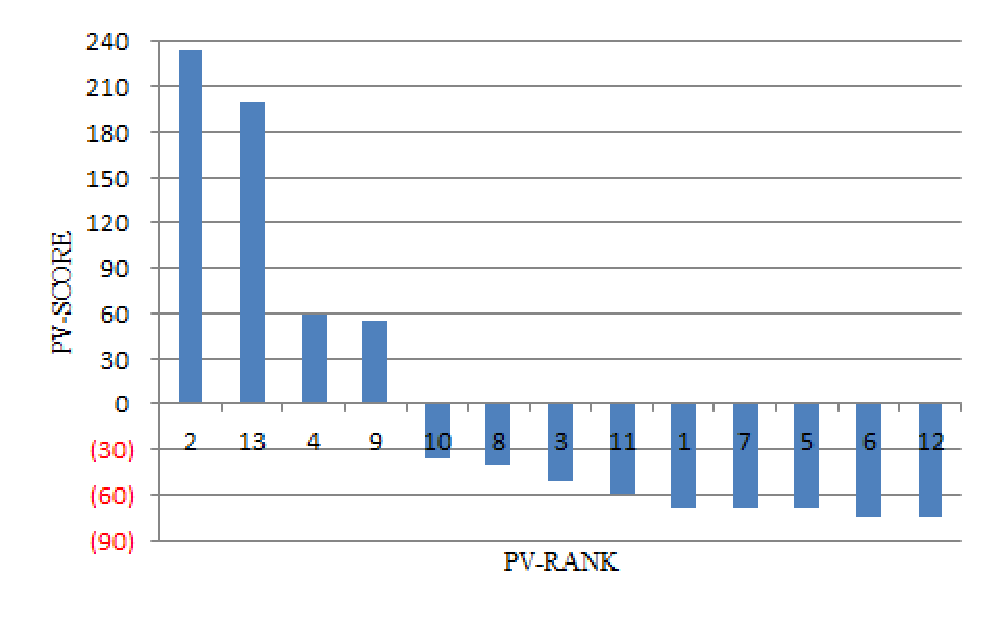
\includegraphics[width=0.99\textwidth,height=5cm]{figures/pv}
    \end{minipage}
    \begin{minipage}[t]{0.5\linewidth}
        \centering
          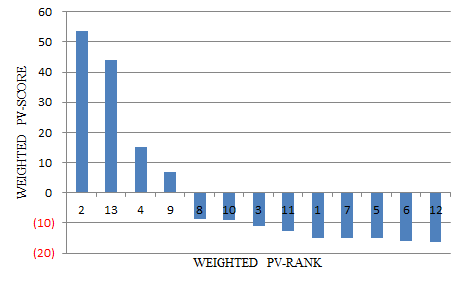
\includegraphics[width=0.99\textwidth,height=5cm]{figures/weightedpv}
    \end{minipage}\caption{序对投票准则下的搜索排名聚合(\textbf{左})与加权排名聚合(\textbf{右})}\label{fig:pvaggregation}
\end{figure}

\chapter{排名收敛}
传统数值迭代方法,如牛顿法、高斯-赛德尔方法、超松弛迭代、雅克比方法和幂法,大多根据相邻迭代结果之间偏差界作为判定迭代收敛而终止迭代计算的准则,我们称其为\textbf{数值收敛准则}(convergence in value)。

在网页搜索领域,PageRank是影响搜索引擎排名的一个重要因素,计算网页PageRank分值的方法有多种,幂法是其中应用最广泛的一种,关于PageRank的研究论文达上万篇
\footnote{根据Google Scholar搜索结果,截止2013年03月26日下午16:30,标题中包含PageRank关键词的可下载PDF文献有10,800条。},
然而绝大多数关于PageRank 分值的计算都是基于数值收敛准则。由于PageRank主要应用在网页排名,相比精确分值而言,我们更关心的是各个网页的排名顺序。

Peserico和Pretto在\cite{peserico2007does,peserico2012hits}首次正式给出迭代排名算法的\textbf{$\epsilon$-排名收敛}(convergence in rank)直观性的定义,并提出一些开放性的问题,比如数值收敛与排名收敛是否存在强关联性,链接图的类型对两种收敛准则的影响等。本文旨在解决此类开放性问题,首先从“序”的概念出发,定义一种基于序稳定性的收敛准则,再从数学上严格证明序稳定性与数值稳定性之间的联系。我们将序稳定性收敛准则应用到PageRank算法的计算,从而大幅提升网页排名计算的性能。

\begin{definition}[排列模式]%Permutation Pattern
对于一个长度为$n$的排列$\pi=\pi_1\pi_2\ldots\pi_n$,其中$\pi_i$表示排列中的第$i$个数。比如,在排列$\pi=391867452$中,$\pi_1=3$,$\pi_9=2$。如果排列$\pi$存在一个子列(不必连续)与排列$\sigma$具有相同的相对序关系,则称$\pi$包含$\sigma$,排列$\sigma$称作$\pi$的一个\textbf{模式}(pattern),并记作$\sigma\le \pi$。由于排列$\pi=391867452$中含有子列($91674, 91675, 91672$),则称它含有模式$\sigma=51342$。每个子列都称作$\sigma$的一个\textbf{复本}
(copy)或出现一次$\sigma$。由于$\pi$不包含一个长度为4的递增序列,可以说它不包含模式$1234$。
\end{definition}

\begin{definition}[序关系]
对于非空集合$A$上的二元关系$\prec$,如果
\begin{enumerate}
    \item 对任意的$a\in A$,都有$a\prec a$,则称它满足\textbf{自反性}(reflexive);
    \item 对任意的$a,b,c\in A$,只要$a\prec b,~b\prec c$,都有$a\prec c$,则称它满足\textbf{传递性}(transitive);
    \item 对任意的$a,b\in A$,只要$a\prec b,~b\prec a$,都有$a\prec a$,则称它满足\textbf{反对称性}(anti-symmetric);
    \item 对任意的$a,b\in A$,要么$a\prec b$,要么$b\prec a$,则称它满足\textbf{完备性}(complete)。
\end{enumerate}
如果二元关系$\prec$满足自反性和传递性,则称它是“\textbf{预序}”(pre-order)关系;如果还满足反对称性,则称它是“\textbf{偏序}”(partial order)关系,$A$是“偏序集”(partial order set,poset);如果还满足完备性,则称它是“\textbf{全序}”(total order)关系,也称“\textbf{线性序}”(linear order)或“\textbf{简单序}”(simple order)。
\end{definition}

%根据全序关系,非空集合可以产生唯一的线性链表。
本文在不产生混淆的情况下,使用\textbf{“序关系”}表示$n$ 维实向量,比如$u=(u_1,u_2,\ldots,u_n)^T$ 各元素(实数)之间的全序关系$\le$。
\begin{property}
实数集上的二元关系“$<$”是偏序关系,但不是全序关系;“$\le$”既是偏序也是全序关系。
\end{property}

\begin{definition}[排列]
\end{definition}

\begin{definition}[偏好关系]%preference relation, power law, small world
\end{definition}

\begin{definition}[实数排列]
对于向量$u\in \mathbb R^n$,对向量所有元素按照二元序关系$\le$进行排列,如果逐次记录所有维度上的排名序构成一个新的向量,则称它是向量$u$的“\textbf{序数列}”,记作$\pi(u)$,符号$\pi(u_i)\in \mathbb{R}$表示$u_i$的\textbf{序/排名},$\pi_i^{-1}(u)$表示向量$u$按照“序关系”排在$i$位的元素,元素的数值越小则“序”越大。假设以$u$的序数列为标准,我们称$\pi(u)$为\textbf{“理想序数列”},相应的各个元素的序为\textbf{“理想序”}。
\end{definition}

\begin{definition}[保序映射]
假设$\prec_A$和$\prec_B$分别是定义在集合$A$和$B$上的全序关系,$f:A\mapsto B$是从集合$A$到集合$B$上的一个双射,对任意的$x,y\in A$,如果$x\prec_A y$,则有$f(x)\prec_B f(y)$,那么$f$称作是从集合$A$到集合$B$的一个\textbf{保序映射}(preserving mapping)。
\end{definition}

\begin{definition}
如果向量$u,v\in \mathbb R^n$满足$\big[\pi(u_i)-\pi(u_j)\big]\big[\pi(v_i)-\pi(v_j)\big]>0,~~~\forall 1\le i\ne j\le n$,则称$u$和$v$\textbf{同序},否则称两者\textbf{逆序}。如果存在函数$f:\mathbb{R}^n \mapsto \mathbb{R}^n$,使得$f(u)$与$u$同序,则称$f$是\textbf{保序函数}。
\end{definition}

\begin{example}
对于5维向量$u=(0.2,0.1,0.6,0.5,0.3)^T$,则$0.1\le 0.2\le 0.3\le 0.5\le 0.6$,则$\pi(u)=(4,5,1,2,3)$,而$\pi(u_5)=3$,$\pi_2^{-1}(u)=0.5$。对于向量
\[
    v=(0.4,0.2,1.2,1.0,0.6)^T, ~~~w=(0.3,0.2,0.7,0.6.0.4)^T
\]
它们与$u$相互“同序”。由此可知,对于任意向量$u$,变换
\[
    \begin{array}{l}
      f:u_i \mapsto u_i + a \\
      g:u_i \mapsto \lambda u_i
    \end{array}
\]
其中,$a\in \mathbb{R}, \lambda>0$,则变换$f,g$都是保序的。
\end{example}

\begin{definition}[序距]
对于任意的$u,v\in \mathbb{R}^n$,$\pi(u),\pi(v)\in \mathbb{R}^n$,如果$\delta:\mathbb{R}^n \times \mathbb{R}^n \mapsto \mathbb{R}$满足如下性质:
\begin{enumerate}
\item 如果$u$和$v$同序,则$\delta(u,v)=0$;
\item 如果$u$和$v$逆序,将$v$中元素随机排列构成集合$V$,对任意$v_\alpha\in V$,都有$\delta(u,v)\ge \delta(u,v_\alpha)\ge 0$;
\item 如果以$\pi(u)$为理想序数列,对任意的$i<j<k$,交换元素$\pi_i^{-1}(u)$和$\pi_j^{-1}(u)$的位置(序/排名),得到$u_\beta$,交换元素$\pi_i^{-1}(u)$ 和$\pi_k^{-1}(u)$的位置,得到$u_\gamma$,保持其他元素的位置不变,则$\delta(u,u_\beta)> \delta(u,u_\gamma)$。
\end{enumerate}
则称$\delta$是$u$和$v$的\textbf{序距}(ordinal distance)。
\end{definition}

\begin{definition}[序稳定性与序收敛准则]%Rank Stability

\end{definition}

%\chapter{元搜索引擎}
%元搜索引擎(简称“元搜”)是一种“超搜索引擎”。它通过统一的搜索界面,将用户的检索请求,提交给多个搜索引擎,并将各搜索引擎返回的搜索结果经过滤重、聚类、重排等过程,展示给用户(见图\ref{fig:metase})。接收元搜索引擎检索请求的搜索引擎,称作“源搜索引擎”、“成员搜索引擎”或者“独立搜索引擎”,我们在后文统一称之为“独立搜索引擎”。一般而言,元搜没有独立的爬虫,依赖于独立搜索引擎而存在。
%
%\begin{figure}[ht]
%  \centering
%  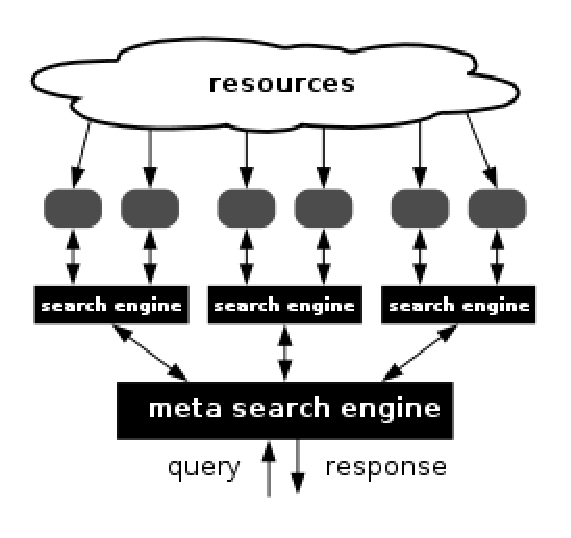
\includegraphics[width=0.5\textwidth,height=5cm]{figures/MetaSE.eps}
%  \caption{元搜索引擎工作流程草图}\label{fig:metase}
%\end{figure}
%
%国外元搜的发展比国内更成熟,无论界面设计,还是搜索技术都有大量可借鉴之处,这里简单介绍几个比较典型的元搜及其基本功能。
%\section{Savvy Search}
%睿智搜索(Savvy Search)是世界上第一个元搜索引擎,由科罗拉多州立大学研究生Daniel Dreilinger开发,1995年3月正式上线。
%睿智搜索运行在五台机器上,三个Sun SpackStation,两个IBM RS 6000s,其设计关注于平衡最大化精度、最小化计算及网络资源消耗两个相互冲突的目标,根据对各个独立搜索引擎长期的观察,确使每次提交给睿智搜索的检索词,依据系统历史统计数据,向最可能返回相关结果的独立搜索引擎提交检索请求,不仅确保精度,还减少了向所有独立搜索引擎提交查询的开销。
%睿智搜索是一个并行检索的元搜索引擎,可调用二十一个独立搜索引擎,检索包括WEB、USENET新闻组、软件、参考工具、人、技术报告等信息。每次最多可同时检索五个搜索引擎的数据库,也可以作为独立的搜索引擎使用。它还支持布尔查询,由于并非所有成员搜索引擎都能正确处理布尔操作符,搜索结果可能并不精确。它还允许用户指定每个搜索引擎返回结果的数目,如选择“聚合结果”选项,系统将对结果集作去重处理。默认情况下,它只显示各个独立搜索引擎前二十条命中记录。另外,它还支持包括中文在内的二十三种语言版本的搜索功能。
%1999年10月14日,CNet网络集团宣布以2200万美元股票和现金组合的形式将其收购,此时睿智搜索已经融合了三百多个网络搜索引擎的搜索结果,月均使用用户达到百万。
%
%\section{Meta Crawler}
%1994年,华盛顿大学研究生Eric Selberg和助理教授Oren Etzioni共同开发出Meta Crawler,并在1995年7月发布。Meta Crawler与Savvy搜索同年开发同年发布,人们常误以为它是世界上第一个元搜索引擎。1995年初,Meta Crawler已经运行在四个AlphaStation工作站上,日均处理几万条查询,给华盛顿大学宽带造成巨大的压力。1995 年夏,两人成立NetBot公司进行商业推广,但是由于没有明确的盈利模式,还需要向独立搜索引擎支付查询费用,不得己将使用权转让给Go2Net。2000年,Go2Net与InfoSpace 合并,虽然Meta Crawler仍提供独立的元搜索服务,地位已是今非昔比。
%Meta Crawler聚合了Google,Yahoo!,Bing,Ask.com,About.com,MIVA,LookSmart和其他主流搜索引擎的结果,提供网页、图片、视频、新闻的搜索服务。在高级搜索页面,用户可以设置最大等待时长(5秒至2分钟)和每个搜索引擎返回结果的最大数目(10、20、30),对各个独立搜索引擎的结果集成,删除重复的URL和死链接,将排序结果以统一的形式显示给用户。
%
%根据Eric Selberg自己的介绍,他们仅仅使用3到5个月的时间开发完成Meta Crawler,其中最复杂的一块就是网络处理,网络协议、并行I/O上占用了绝大部分时间。在开发时两人完全没有考虑过具体的商业模式,只是在发布后才逐渐摸索出一套商业模式:通过在搜索结果中显示独立搜索引擎的推广广告,实现利润共享。Eric认为,元搜面对的问题有很多,主要包括三点:(1)资源发现,能够自动发现新的搜索引擎并将其加入到独立搜索引擎列表;(2)用户认同,把用户的注意力从独立搜索引擎吸引到元搜;(3)商业模式,很难找到一个让所有独立搜索引擎提供商都满意的商业模式。
%
%\section{Dogpile}
%1996年,Aaron Flin创立了Dogpile,11月正式投入运营。1999年8月,以价值5500万美元的股票和现金作价卖给Go2Net,使得Go2Net旗下同时拥有了两个最受欢迎的元搜索引擎:Meta Crawler与Dogpile。2000年8月,InfoSpace与Go2Net集团合并,但Meta Crawler和Dogpile继续分开运营。2002年初,InfoSpace又以1,000万美元的低价收购Excite和Web Crawler,以麾下四个最著名的元搜索引擎独霸元搜索市场。
%
%Dogpile聚合了顶级搜索引擎Google、Yahoo!、Bing、Ask.com和About.com的搜索结果,并在2005年4月、2005年7月、2007年4月同匹兹堡大学(Pittsburgh University)、宾夕法尼亚大学(Pennsylvania State University)、昆士兰科技大学(Queensland University of Technology)研究人员合作,使用上万个查询词,估计几个顶级搜索引擎搜索结果的重复率情况。研究发现,主要搜索引擎(包括Google,Yahoo!,Ask,Bing)搜索结果的重复率低于4\%,2007年的研究结果甚至低于1\%,从而以此证明任何单个独立搜索引擎都不能完全满足用户的检索需求,元搜的存在是有价值的,它可以弥补独立搜索引擎覆盖率不足的问题,聚合多个独立搜索引擎的搜索结果,给用户更多相关的结果。
%
%\section{Excite}
%1994年,斯坦福大学(Stanford University)的Graham Spencer,Joe Kraus,Mark Van Haren,Ryan McIntyre,Ben Lutch和Martin Reinfried共同创立了Excite,提供包括门户、搜索引擎、电子邮箱、即时信息等多种在线服务。1994年7月,国际数据集团(International Data Group)向其投资10万美元用于开发一个在线服务网站,并于1995 年12月正式上线。1996 年1月,George Bell(错失过以75万美元收购Google的良机)以CEO的身份加盟Excite,并主持收购两个搜索引擎Magellan和WebCrawler。
%1996年4月4日,Excite首发200万股股票。由于经营不善,1998年3月31日其净损失竟达到近3千万美元,1999年1月19日@Home Network公司以67亿美元的价格将其收购,并组建新公司Excite@Home,融合@Home的高速网络服务和Excite搜索及门户网站,专注于提供个性化的网络内容服务。由于接二连三的商业决策失误,2001年9月13日Excite@Home申请破产保护,期间Iwon.com与InfoSpace联合投中Excite域名和品牌。2001年12月16日,Iwon.com启用新的Excite门户,并更名为Excite网络公司,继续经营Excite、iWon和另一个门户MyWay。InfoSpace则拥有和运营Excite的网络搜索部分。
%2004年3月Ask Jeeves(如今的Ask.com)将Excite网络公司收购,并在2005年,与InfoSpace就美国区Excite业务达成和解,双方共同承担市场成本、共享Excite 搜索业务的利润。
%
%\section{Web Crawler}
%1994年4月20日,由华盛顿大学(Washington Uiversity)学生Brian Pinkerton开发的Web Crawler发布上线,成为世界上第一个提供全文搜索的网络搜索引擎。1995 年6月1 日,美国在线将其收购,又在1997年4月1日转手卖给Excite,2001年Excite@Home破产后又将其出售给InfoSpace。最初,Web Crawler拥有独立的抓取程序和网页数据库,其主要收入来源于搜索结果页面投放的广告费,在并入InfoSpace以后,作为元搜索引擎向用户提供搜索服务。
%
%\section{Vivisimo}
%
%
%\section{Ixquick}
%Ixquick是David Bodnick于1998年研发并推出的一个元搜索引擎,自称是全球最大中介搜索引擎,目前支持14个搜索引擎的搜索结果。2000年,Ixquick被一家荷兰公司Surfboard Holding B.V收购。Ixquick背后的独立搜索引擎包括:Teoma,EntireWeb,All the Web,Ask,Bing,Cuil,Exalead,Gigablast,Lycos,AltaVista,WiseNut,LookSmart,Netscape,Open Directory, Qkport, Wikipedia,Statesman,Yahoo与Blekko,不含Google。
%
%2006年6月27日,Ixquick声明删除用户详细浏览信息,并保证在48小时内清除提交搜索的用户IP地址和其他个人信息。2009年1月28日宣布完全停止对用户IP地址的记录。
%截止2010年1月,Ixquick已经处理了12亿次查询请求。根据Ixquick公司背景介绍,它是世界上隐私保护做得最好的搜索引擎公司,从2006年起,开始专注对用户隐私的保护,做到不记录用户IP地址、cookies,不搜集而且不与第三方分享用户个人数据,提供安全的、加密的HTTPS/SSL连接。
%
%Ixquick直言提供相似搜索服务的搜索引擎,包括Google、Yahoo!和Bing,以及元搜索市场上,拥有三家马车的InfoSpace是其主要竞争对手。它目前还未上市,在过去的5年里(2006年起)一直都是盈利的,资金充裕,其盈利模式并无特别之处,在搜索结果页面显示相关的“赞助结果”,按照点击次数向广告客户收取费用,但每页显示的“赞助结果”不超过3条,而且全部放到搜索结果的首尾两端。
%
%由于Ixquick难以记忆和拼写,该公司于2009年启用新的域名Startpage\footnote{See http://www.startpage.com/}。有消息称,Ixquick 正在开发邮件服务系统。
%\section{Mamma}
%1996年,由加拿大人Herman Tumurcuoglu开发的网站Mamma.com
%\footnote{\href{http://www.mamma.com/}{http://www.mamma.com/}}
%正式发布上线。2005年12月22日,Mamma.com以1590万美元收购一家搜索技术公司Copernic,并发行238万股股票。Mamma.com 能够有效整合多个顶级搜索引擎的搜索结果,赢得“搜索引擎之母”的称号。它支持常用检索语法在不同搜索引擎之间的转换,还提供通过Email订制搜索结果的特色服务。Mamma.com还是一个广告网络公司,通过在线推介创收。
%
%\section{Kartoo}
%2002年04月25日,Laurent Baleydier和Nicholas Baleydier两兄弟联合开发的Kartoo\footnote{See http://www.kartoo.com/}上线,它是一个可视化元搜索引擎,以图形界面的形式展示搜索结果,通过关键词建立语义连接,将搜索结果生成一个聚类图,方便用户选择、缩小搜索范围。2010年1月,由于不明原因关闭。
%
%Kartoo使用的可视化技术是Laurent团队研究三年的成果,使用球形结点代替搜索结果条目,并通过球形节点的大小反映页面的重要程度。Kartoo最引人注目的地方在结点间的语义连接,如果搜索条目之间存在连接,则使用语义关键词标示节点之间的连线。Kartoo易于使用,并且富有趣味性,代价就是加载过慢。
%
%与国际市场形成鲜明对比,国内元搜市场鲜见成功的案例。我们下面介绍国内几个昙花一现的元搜:

%\subsection{比比猫}
%2005年1月1日,新加坡人朱明谦(Kim Choo)和李昌日联合创立了比比猫(Bbmao),并在2006年02月发布上线,它是中国第一家聚类元搜索引擎,通过聚类技术和个人网络收藏夹改善搜索结果。
%
%朱明谦对中国市场的分析可以归纳为以下几点:(1)中国搜索引擎市场差异化程度比较低,元搜的机会比较大。传统搜索引擎公司在底层搜索技术投入巨大,Bbmao 则更注重以上层的数据处理技术、智能搜索技术求生存。(2)大多数元搜没有核心技术,仅仅是整合其他搜索引擎的结果。只要有核心技术,公司就一定有价值,而Bbmao的核心技术就是聚类技术。(3)与独立搜索引擎合作共赢,独立搜索引擎提供搜索结果和竞价排名广告,元搜借着竞价排名广告收入分成。在06年,Bbmao的首席财务执行官Bill Milewski透露,Bbmao的盈利主要靠广告,并协议和Google等各大搜索引擎对广告利润分成。Bbmao期望成为一个社会化搜索引擎网站,其根本是发挥Web 2.0的内核——个人应用,靠用户改善搜索结果,就像Google通过搜索结果的点击改善排名。其特点可以归结为以下几点:
%\begin{itemize}
%  \item 资源聚合:同时提供Google,百度,雅虎,搜狗和爱问五大搜索引擎组合搜索或单个搜索结果,搜索结果排名是根据网页在各个搜索引擎中结果中出现的次数及排名来确定的,并明确标示各条结果在相应搜索引擎中的排名信息;
%  \item 聚类:在搜索结果页面左侧,呈现聚类列表,由用户点击选择目标类别,优化查询结果;
%  \item 去重:采用公司开发的FeatureMatch技术;
%  \item 快照:提供搜索结果预览;
%  \item 网络搜藏夹:注册用户享有的服务,方便用户收藏和共享,期望借此跟踪用户习惯,更好地为用户提供聚类结果,打造社会化搜索圈。
%  \item RenqiScore:使用人气得分技术向用户推荐高品质的相关会员,建立属于用户自己的交际网,还可以通过邀请朋友扩大交际圈。
%\end{itemize}
%
%2005年,Myspace创始人Brad Greenspan完成对Bbmao的注资,成为BroadWebAsia(BWA)集团在中国的第一笔投资。2006年3月,Bbmao的流量达到每天2万至3万,8月份超过7 万。Bbmao创建以后赢得的诸多赞誉,它启动“比比猫公益搜索”平台,以期打造互联网企业社会责任新方向。目前,Bbmao已经倒闭。Bbmao倒闭的原因有(1)用户习惯:它无法扭转已经习惯使用百度和Google的用户习惯。(2)它只是进行了非经营性网站的备案,并未获得经营性网站信息许可证,不能从事盈利性商业活动。(3)盈利模式单一:它主要与合作伙伴间的点击付费分成。
%
%\subsection{万纬}
%由上海万纬信息技术有限公司在1999年12月推出,是中国第一个元搜索引擎,集成了包括Google,Yahoo!,HotBot,AltaVista等8个英文搜索引擎,中文雅虎,搜狐、新浪、中文Excite、中文Google等12个中文搜索引擎,起正式版本2002年发布,功能比较完善。
%
%万纬搜索提供的高级搜索功能包括:(1)允许布尔查询,支持AND/OR;(2)结果排列方式有四种选择,包括相关度、时间、网站分类、引擎;(3)选择最大等待结果的时间,7秒到1分钟,默认20秒。(4)允许设置显示的查询结果个数,10到200个,默认为20个。遗憾地是,万纬在2007年7月份就已经停止查询服务。
%
%\subsection{搜乐}
%搜乐是广州明智科技有限公司推出的一个元搜索引擎。目前,搜乐整合了Google、百度、必应、搜狗、有道、搜搜和中搜等搜索引擎的搜索信息,并支持自动去重。
%主页功能显示,搜乐支持对网页、图片、视频、文档、新闻和微博的搜索,其中文档搜索包含的格式有Doc、XLS、PPT、PDF、RTF和TXT。
%
%在“设置”中可由用户指定(1)界面语言,包括中文繁体和简体。(2)搜索语言可不限。(3)每页显示结果3到100条。(4)是否在结果页中显示“推广”项;(5)是否允许在结果页中显示“赞助链接”。
%
%高级选项模仿了部分Google高级搜索的设置,添加对关键词出现位置的设定,包括文档的任何地方、仅标题、仅正文、仅URL和指向文档的链接。此外,它还支持对单个网站的搜索。目前搜乐不支持任何搜索,只有图片和视频展示页面。根据58同城招聘信息,明智科技正在招聘.NET软件工程师(2012年4月11日)和网站美工(2012 年3月21 日),组建创业团队。该公司主营产品是蓝月亮VOD点播系统。
%
%\subsection{名捕}
%名捕根据搜索类别,提供不同的资源列表方便用户选择,见下表:
%\begin{table}[htbp]
%\centering
%\begin{tabular}{|c|c|}
%    \hline\hline
%    搜索类别 & 资源网站列表\\
%    \hline
%    网页 & 百度、搜搜、搜狗、有道、中搜、必应、雅虎、谷歌、即刻\\
%    图片 & 雅虎、新浪、必应、搜狗\\
%    音乐 & 新浪、搜狗、雅虎、狗狗、搜搜\\
%    视频 & 新浪、土豆、优酷、搜搜、搜狗、谷歌、乐视\\
%    软件 & 天空、Enet、华军、百度、ZOL、Pchome、新浪\\
%    新闻 & 谷歌、有道、搜搜、必应、百度、搜狗\\
%    知识 & 知道、雅虎、百科、搜搜、搜狗\\
%    博客 & 搜搜、百度、有道、爱问、奇虎、搜狗、谷歌\\
%    论坛 & 谷歌、中搜、奇虎、贴吧、搜搜\\
%    词典 & 搜搜、爱词霸、海词、有道、沪江、词酷\\
%    财经 & 和讯、金融界、谷歌、搜牛、中金\\
%    购物 & 谷歌、有道、淘宝、当当、卓越\\
%  \hline
%\end{tabular}
%\end{table}
%
%它只提供搜索引擎的切换,不提供结果排名聚合。从根本上来讲,它只提供了针对各个搜索类别比较权威的站点,供用户挑选。此外,名捕还在首页提供了几个不错的资源——搜索大全、儿歌大全、晨曦五笔、绝妙好词。
%
%\subsection{P搜}
%P搜是刘洪照历经四年研发的成果,它聚合了百度、Google、Yahoo!、搜狗、有道、搜搜和必应的搜索结果,经过去重,重排,缩小搜索范围,精确查找信息。
%根据其本人介绍,第一版搜鸿元搜索引擎(sohong.cn)由于技术瓶颈问题,一直没突破速度限制,搜索耗时略长。在2009年4月份他重写搜鸿,突破了技术瓶颈,并陆续添加竞价排名和后台管理模块,并易名为新牛元搜索(ccniu.com)。后受到115聚合搜索的影响,历时一周对新牛改写,实现了各个模块的松耦合,并通过API整合各个模块,
%
%2009年9月升级到第二版。2010年初新牛上线,放弃服务端处理模式,改用Ajax模式,速度比以前要慢,但节省服务器开支,由于没有独立服务器,Ajax版本超过两秒,原服务端处理在1秒以内。至2011年2月,历经5次代码重写,多次更新,新牛算法趋于合理,搜索结果排序更加人性化。2011年5月8日改版并易名为P搜,采用镜像psou.cn。
%
%\subsection{马虎聚搜}
%马虎聚搜是BroadWebAsia(BWA)集团在中国投资的第一家互联网公司,提供基于搜索引擎的多种互联网服务。马虎聚搜声称经过技术测试,国内通用搜索引擎在搜索结果前两页当中,重复率约占5-16\%。该公司拥有独特的FeatureMatch技术,可以大幅减少搜索结果中的重复信息。(FeatureMatch——Bbmao)
%
%搜索发现,基本上和百度的搜索结果一样,不同之处在于马虎聚搜会过滤掉百度文库、百度翻译、能够提供直接下载的搜索结果条目,并在每个搜索结果条目前加注序号。如切换到独立搜索引擎,会自动弹出对应的搜索引擎搜索结果页面,若切换到Google、Bing,还会出现中文乱码。支持收藏和预览功能,但最多返回10页搜索结果。对音乐、图片、视频的搜索直接跳转到百度的搜索页面。
%
%\subsection{佐意}
%佐意网的前身是一佐网络,始建于1998年3月,2007年3月正式更名为佐意网,并启用新域名。佐意是一个集成搜索引擎,提供网页,新闻,软件,游戏,动画,音乐,影视,地图等信息的搜索,能够自动屏蔽掉色情木马不良网站,减少用户的烦恼。2010年10月11日,佐意网终止搜索服务,转为一个以BLOG为主,并提供相关查询的综合性网站。2011年7月1日,佐意官网宣布停止运营,终止所有服务。
%
%\subsection{Juxit}
%Juxit是Reuben Boyd 于2004年创建和发布的,声称是第一个聚合了中英双语的元搜索引擎。它聚合了Google中文,Yahoo中文,百度,搜狗,MSN,Wisenut 和 Looksmart 的搜索结果。Juxit包含购物、旅行、新闻、图片、视频和音频搜索,并提供预览功能。它支持免费的、按点击次数收费的广告,并推出联盟计划(affiliate program),向广告客户支付转介佣金。此外,它还允许广告穿插到搜索结果中。目前,Juxit已经停止运营。
%
%目前中国国内还出现过很多其他元搜,我们将它们全部收录于表~\ref{tbl:cnmetase}。
%\begin{table}[htbp]
%\centering
%\caption{中国元搜索引擎目录}\label{tbl:cnmetase}
%\begin{tabular}{|l|l|l|l|l|}
%    \hline\hline
%    名称 & 介绍 & 发布时间 & 状态\\
%    \hline
%    \href{http://www.bioon.com/multisearch.htm/}{生物谷} &  张发宝开发,搜索时同时展开多个页面 & 2001年10月 & 正常\\
%    \hline
%    \href{http://www.suotianxia.com}{索天下} &  -- & 2006年12月14日 & 关闭\\
%    \hline
%        &  华南师范大学附属中学的叶古于2003年开发,采用CooRank & & \\
%    \href{http://coo.hsfz.net/fish/}{MetaFisher} & 自动分网页评级系统优化排序,CooWord2Beta关键词 & 2003年 & 关闭\\
%        & 析归纳算法增加搜索深度和广度,CooSimil滤重 & & \\
%     \hline
%        & 提供了Google+百度,Google+Yahoo!,Google+Yahoo! & & \\
%    \href{http://www.xisoso.com/}{Xisoso} &  三种组合的搜索结果,搜索结果还提供del.icio.us  & -- & 关闭 \\
%        & 标签和天天网摘(365Key),还支持自动聚类功能 & & \\
%    \hline
%    \href{http://www.baidugoo.com/}{Baidugoo} &  -- & -- & 关闭\\
%    \hline
%    \href{http://www.bydou.com/}{北斗搜索} &  深入搜索、相关搜索、可评价结果 & -- & 关闭 \\
%    \hline
%    \href{http://www.ejear.com/}{壹家搜} &  聚合百度、Google中文、Yahoo!中文的搜索 & & \\
%        & 结果,据称对相似结果的处理有其特色 & 2005年11月 & 正常\\
%    \hline
%    \href{http://www.bbmao.com/}{比比猫} &  聚类、在线收藏共享 & -- & 关闭\\
%    \hline
%    \href{http://www.hensou.com/}{狠搜} &  -- & -- & 关闭\\
%    \hline
%    \href{http://www.kwindsoft.com/k-metasearch/}{K风元搜索} &  聚合、收藏功能 & 2007年01月02日 & 关闭\\
%    \hline
%    \href{http://cn.xooda.com/}{Xooda中国} &  支持16个国家和地区的搜索,而中文支持Google、&&\\
%        & 百度、中文雅虎、爱问、搜狗等10多个搜索引擎 & 2007年02月16日 & 关闭\\
%    \hline
%    \href{http://www.seekle.cn/}{Seekle} &  聚合百度、Google、搜狗、Yahoo!的搜索结果 & 2007年12月30日 & 关闭\\
%    \hline
%    \href{http://www.pifa.us/}{PIFA} &  -- & 2008年01月13日 & 关闭\\
%    \hline
%    \href{http://www.sohong.cn/}{搜鸿元搜索} &  艺鸿开发,后易名为搜牛、P搜,支持去重、 &&\\
%        & 重排、预览、收藏等功能,使用方便快捷 & 2008年02月19日 & 正常\\
%    \hline
%        & 基于Ajax技术,聚合谷歌、百度、雅虎、&&\\
%    \href{http://www.metasoo.cn/}{觅搜} & 一搜、搜狗、有道等搜索引擎搜索结果 & -- & 正常\\
%        & 允许用户自行设置各搜索引擎权重 & & \\
%    \hline
%    \href{http://www.deyeb.com/}{Deyeb} &  董一萌开发的社会化元搜 & -- & 关闭\\
%    \hline
%    \href{http://www.soseen.com/}{搜星} &  聚合百度、搜狐、新浪、Google等搜索引擎,可搜索精选网址 & -- & 关闭\\
%    \hline
%    \href{http://www.1qiso.com/}{一起搜} &  自称全球最大中文元搜,聚合12个中外搜索引擎结果 & -- & 关闭\\
%    \hline
%    \href{http://www.jopee.cn/}{Jopee} &  聚合百度、Google、搜狗、必应、有道、Ask,简单切换 & -- & 正常\\
%    \hline
%        & 聚合百度、Google、搜狗、雅虎和中搜,提供网页、 & &\\
%    \href{http://www.someta.com/}{搜魅} & 资讯、图片、网站查询,宣称是最优秀的中文元搜索 & 2009年 & 正常\\
%        & “搜魅聚合”等于是百度搜索 & & \\
%%    \hline
%%    \href{http://www.mangken.com/}{芒肯} &  -- & -- & 关闭\\
%%    \hline
%%    \href{http://www.souk.cn/}{搜客} &  -- & -- & 关闭\\
%%    \hline
%%    \href{http://www.yok.com/}{YOK} &  -- & -- & 关闭\\
%%    \hline
%%    \href{http://www.souk.cn/}{搜客} &  -- & -- & 关闭\\
%%    \hline
%%    \href{http://www.koooi.com/}{酷爱} &  -- & -- & 关闭\\
%  \hline
%\end{tabular}
%\end{table}
%
%\subsection{市场层面}
%从用户使用的习惯来看,中国大多用户已经习惯使用单个搜索引擎比如百度、Google,查询所需信息。目前,由于Google退出中国市场,将服务器移到香港,但时断时续的状态导致用户分流,这就部分造就了如今百度一家独大的局面。
%
%根据iResearc的统计数据,2012年2月Google全球搜索引擎市场份额从1月份的75.9\%下降到72.1\%,同时Yahoo!的市场份额则从11.1\%上升到16.5\%。即便真如Google前CEO Eric Smith所言,称Google实际市场份额是包含了一部分垂直搜索引擎市场的份额的,但Google行业龙头老大的地位短时期内是无法撼动的。
%
%从易观国际在2011年第四季度的数据可以看到,百度在中国搜索引擎市场上的份额达到78.3\%,而处于第二位的Google则只有16.7\%,搜狗、搜搜等其他搜索引擎的市场份额之和只有5\%。这种格局同iResearch全球搜索引擎市场格局颇为相似,即一家独大,在中国,百度处于绝对垄断地位。相对PC机搜索市场而言,中国无线搜索市场分布则比较均匀,但百度的份额仍然是最大的一块。
%
%iResearch在2011年底预计中国搜索引擎市场规模到2013年将达到438亿元人民币,而根据易观国际在2010年的预测,到2013年市场规模将达到313亿元人民币,虽然二者相差将近100亿,但从整体趋势来看,搜索市场增长的潜力是巨大。
%
%在这个巨头环立的市场中,元搜要想生存、获得一席之地,首先要有有明确的用户群和市场定位,推崇用户体验至上;其次,由于元搜会分走独立搜索引擎的部分流量,影响其广告业务,应努力寻找同独立搜索引擎合作的结合点,尽可能营造计较有利的发展环境,打消独立搜索引擎对元搜的戒心,避免成为众矢之的。如2008年4 月7日,李彦宏到上海交大演讲。在互动时有学生提到使用“百Google度”同时搜索百度和Google,李彦宏称“元搜索没有生命力”,然而给出的理由却很牵强,“元搜索可以同时查询多个搜索引擎的站点,但用户不需要那么复杂的结果,而且相当多的人习惯了用百度”,并奉劝创业者不要往视频搜索上“撞”。
%
%\subsection{技术层面(智能选择、去重、聚类、推荐、重排)}
%市场再大,没有核心技术的互联网公司终究无法在这个市场立足,元搜更需要核心技术的支撑。通过分析,国内元搜基本可以归为两种模式:
%\begin{itemize}
%  \item 框架调用:为用户提供在不同搜索引擎之间进行快速切换,基本无核心技术,容易复制;实际上也不能归为元搜的范畴,没有什么参考价值。
%  \item 聚合调用(直接抓取或API调用)——用户一次提交,系统把多个独立搜索引擎搜索结果,经过滤重、重排等处理,返回更为合理的聚合结果。其中,虑重、重排等技术是核心,难以复制。
%\end{itemize}
%第2种模式被普遍认可,它主要存在以下几个问题:
%\begin{itemize}
%  \item 比使用单个独立搜索引擎查询所需时间更长
%  \item 处理高级检索时,需要将检索语句转换为不同独立搜索引擎的标准格式,转换效果不佳并影响到搜索的效率
%  \item 搜索结果依赖于独立搜索引擎数据库的大小、数据的质量
%  \item 只能从独立搜索引擎数据库中获取搜索结果的有限信息,如排名、摘要信息等,影响搜索结果排名的可信性
%  \item 由于部分独立搜索引擎的盈利模式的特殊性,导致其搜索结果中出现竞价排名的商业广告,智能识别出其中的“赞助广告”是一个不小的挑战。识别出不相关的结果页面,如包含木马病毒、色情信息的网页或网站对于改善用户体验是十分重要的,而实现这一目标难度不小
%  \item 由于不同搜索引擎对搜索结果的显示格式也是不同的,以一种统一的方式聚合异构的搜索结果展示给用户,处理起来比较复杂,也是影响搜索效率的又一个障碍
%  \item 元搜经常需要批量访问独立搜索引擎的数据库,但由于各主流搜索引擎对访问都设置了上限,信息的查全率会受到很大影响
%  \item 随着访问量的增加,服务器端流量、数据处理的压力明显增加,因此硬件要求颇高
%\end{itemize}
%元搜是为弥补传统搜索引擎的不足而出现的一种辅助搜索工具。因此,必须从数据库选择、查询分派、文本选择、虑重、结果聚合、排名和显示等环节寻求突破,而且这些也是未来元搜研究的重点。
%
%\subsection{法律层面}
%由于元搜没有独立的数据库,需要在用户提交查询以后,选择并抓取独立搜索引擎的数据库。显然,元搜受制于人,可能会由于频繁抓取独立搜索引擎的数据库,影响独立搜索引擎正常服务,或增加其服务成本而面临诉讼风险。这是否又是一桩“只需州官放火,不许百姓点灯”的经典案例呢?具体的互联网数据信息的访问是否受限,可查询相关法规。
%
%\subsection{国内环境的特殊性}
%在中国搜索市场上,曾经出现过很多元搜索引擎,有些还很优秀,比如Bbmao、万纬,但后来由于不明原因陆续倒闭。其他类型的元搜多是单人开发,核心技术几乎为零,从界面设计到服务性能都与国外成熟的元搜相差甚远,甚至还有一些打着元搜的旗号,使用小偷程序,安装恶意软件,给用户留下很差的印象。因此,若要在中国推出元搜,让更多用户了解元搜的角色和价值、依赖单个搜索引擎的局限性、遗漏重要信息的代价、重拾用户对元搜的信心是首先要做的工作。
%
%另一方面,由于国内对知识产权保护不力,产品一经推出会即刻产生一批跟风者,这种良莠不齐的混乱状况,会给产品形象带来很大的冲击。因此,产品一定要有特色,并有明确的目标受众,能够明显区别于其他类似产品。由于国内众多企业道德问题饱受公众质疑,因此一个坚决抵制不良信息,努力呈现高品质内容,尽力追求企业良知的搜索引擎公司一定是大众所渴望的,也一定可以走得更远。
%
%\subsection{商业模式}
%在早期,搜索引擎多作为技术提供商,通过为其他网站提供搜索服务收取服务费。2001年,互联网泡沫破灭后,多转向竞价排名的方式。现在主流搜索引擎商业模式(Google的AdWords、百度的竞价排名)由是Bill Gross提出的,“在搜索结果页面显示广告,根据用户点击向广告客户收费”。该模式有两个特点:一是点击付费(Pay Per Click,简称PPC),用户不点击则广告客户不用付费;二是竞价排名,根据广告客户的付费多少给结果排名。
%
%2003年6月,Google推出一种免费的广告计划AdSense,它是一种面向站长的广告服务。网站发布者为访客提供Google网页和网站搜索功能,借由在搜索结果页面投放Google 广告以获取收益。目前,各大搜索引擎已经开始使用这种模式。
%
%元搜依赖独立搜索引擎而存在,从搜索业务的角度来看,元搜与独立搜索引擎是竞争关系。由于市场份额多被少数独立搜索引擎瓜分殆尽,元搜要在这种不对等的关系中生存和发展,必须提出一种既不会伤及独立搜索引擎利益,又能够持续提供搜索业务的方案,即与独立搜索引擎合作。元搜同独立搜索引擎该如何合作,国外元搜市场比较成功的商业模式,比如InfoSpace 公司可以为我们提供一些借鉴。
%
%InfoSpace公司通过旗下的三个元搜索引擎——Dogpile, WebCrawler, MetaCrawler向用户提供搜索服务,是一个上市公司,因此需要按规定定期发布公司相关信息。
%2012年3月9日,InfoSpace发布报告,在Business小节中披露,Google, Yahoo!, Bing和其他搜索引擎被InfoSpace称作内容提供商(Content Providers),并且如果部分内容提供商,如Google,Yahoo!向其支付内容发布的费用,则称它们为搜索客户(Search Customer)。
%
%在Search Revenue Source一节中有记录,其主要收入来自内容提供商向其搜索服务中投放的付费广告。广告客户根据用户点击向独立搜索引擎支付费用,InfoSpace 则从中提成。报告中还披露,在2010年和2011年,Google和Yahoo!两家公司占其全部收入来源95\%以上,而其中Google占绝大部分。报告坦言,如若这两家公司减少面向InfoSpace 的业务,或者对之前协议的价格产生异议的话,必然会对InfoSpace的业务和财务构成造成巨大冲击。

%\chapter{Academic Search Engine}
%\chapter{Shopping Search Engine}

%-------------ranking theory
\part{数据挖掘与机器学习}
数据挖掘,又称知识发现(Knowledge Discovery in Database, KDD),是一门交叉学科,包括人工智能(Artificial Intelligence, AI)、机器学习(Machine Learning, ML)、模式识别(Pattern Recognition)、统计学、 数据库、可视化等技术,能够从数据源(如数据库、文本、图片、因特网等)中揭示出\textbf{隐含的,并有潜在价值的模式或规律}的复杂过程。


%\ornamento
\chapter{回归分析}
回归分析是一种监督型学习方法,从给定观测数据$\{x_i,y_i\}_{i=1}^n$中,训练出一个回归模型$f(\omega,x)$,建立起自变量$x\in \mathbb{R}^m$与因变量$y\in \mathbb{R}$之间潜在的因果关系。回归模型在观测数据集上的回归误差可用于衡量模型对数据拟合的效果:
\begin{equation}
    \mathbb{L}(\omega) = \frac{1}{n} \sum\limits_i L(y_i,f(\omega,x_i))
\end{equation}
其中,$L(y,f(\omega,x))$表示回归模型$f(\omega,x)$的预测结果与因变量真实值$y$的偏差。一般地,偏差越大则拟合效果越差。

为了实现对数据集的最佳拟合,我们通过最小化(规则化的)经验损失函数估计模型参数:
\begin{equation}
    \hat\omega = \argmin\limits_{\omega}~\mathbb{L}(\omega) + \lambda \mathcal R(f)
\end{equation}
其中,第二项是规则化项,$\lambda$表示权衡因子,体现模型精度与模型复杂度之间的权衡。

如果回归模型是线性的,则称回归分析为\textbf{线性回归}。在训练回归模型时,如果使用的损失函数或规则化项不同,则学习得到的回归模型亦不同,常见的损失函数有:
\begin{itemize}
  \item 平方损失:
  \begin{equation}
    L(y,\hat y) = (y-\hat y)^2
  \end{equation}
  \item 绝对值损失:
  \begin{equation}
    L(y,\hat y) = |y-\hat y|
  \end{equation}
  \item $0-1$损失:
  \begin{equation}
    L(y,\hat y) = \ind(y\ne \hat y)
  \end{equation}
  \item 合页损失(Hinge Loss):
  \begin{equation}
    L(y,\hat y) = \max(0, 1-y \hat y)
  \end{equation}
  \item 伯努利负对数损失(Bernoulli Negative Log-likelihood Loss):
  \begin{equation}
    L(y,\hat y) = \log (1+e^{-y\hat y})
  \end{equation}
  对于二元分类,伯努利负对数损失实际上就是$0-1$损失的一个上界。
\end{itemize}

如果损失函数是平方损失函数,对经验损失函数做\textbf{Tikhonov 规则化},也就是$\mathcal{R}(f)=\|\omega\|_2^2$,对应的回归分析方法称作\textbf{岭回归}
(Bridge Regression);如果规则化项是$\mathcal{R}(f)=\|\omega\|_1$,则对应回归分析方法称为\textbf{Lasso}\cite{tibshirani1996regression}。

\section{线性回归}
1805年,法国数学家Adrien-Marie Legendre发明了\textbf{最小二乘法}(Least Squares Method),但一直不为人知。1809年,德国数学家Carl F. Gauss在《天体运动论》一书中对最小二乘法做了介绍,并于1829年从统计学的角度证明最小二乘法的优越性:最小二乘解在所有无偏估计中方差最小(Gauss-Markov定理)。

给定一组数据$\textit{S}=\{x_i,y_i\}_{i=1}^n$,其中$x_i\in \mathbb{R}^m$,$y_i\in \mathbb{R}$,假设目标值与输入值之间的关系可以用下面的等式表示:
\begin{equation}
    y_i = f(\omega,x_i) + \epsilon_i
\end{equation}
其中,$\epsilon_i$表示误差项,可以捕获随机噪声。假设预测误差项$\epsilon_i$服从均值为0,方差为$\sigma^2$的正态分布(高斯分布、钟形分布),并且相互独立(i.i.d),
\footnote{独立同分布:Independent and Identically Distributed,i.i.d}
记作$\epsilon_i\sim N(0,\sigma^2)$,那么它们的概率密度函数为
\begin{equation}
    p(\epsilon_i) = \frac{1}{\sqrt{2\pi}\sigma} \exp\big\{-\frac{\epsilon_i^2}{2\sigma^2}\big\}.
\end{equation}
根据正态分布的性质可知
\begin{equation}
    p(y_i|x_i;\theta) = \frac{1}{\sqrt{2\pi}\sigma} \exp\big\{-\frac{(y_i - f(\omega,x_i))^2}{2\sigma^2}\big\},
\end{equation}
可简记:$y_i|x_i;\theta\sim N(\omega^T x_i,\sigma^2)$。

我们使用最大似然估计,最大化对数似然函数
\begin{equation}
    \begin{array}{lll}
      L(\theta) & = & \log \prod\limits_i p(y_i|x_i;\theta), \\
       & = & \sum\limits_i \log \frac{1}{\sqrt{2\pi}\sigma} \exp\big\{-\frac{(y_i - f(\omega,x_i))^2}{2\sigma^2}\big\}, \\
       & = & \sum\limits_i \log \frac{1}{\sqrt{2\pi}\sigma} - \frac{1}{2\sigma^2} \sum\limits_i (y_i - f(\omega,x_i))^2, \\
    \end{array}
\end{equation}
等价于最小化误差平方和:
\[
    \min\limits_\omega~~L(\theta) = \sum\limits_i \big[y_i - f(\omega,x_i)\big]^2,
\]
从理论上证明了最小二乘法合理之处。假设回归模型是线性的,则有
\begin{equation}
    \min\limits_\omega~~L(\theta) = \sum\limits_i (y_i - \omega^T x_i)^2 = (y-X\omega)^T (y-X\omega).
\end{equation}
目标函数是$\omega$的一个凸函数,根据极值必要性条件可知
\[
    X^T X \omega = X^T y.
\]
我们可以证明,最小二乘法恒有且存在唯一解的充要条件是$\textit{rank}(X)=\textit{m}$。此时,最小二乘法有解析解(Closed Form Solution):
\begin{equation}
    \hat \omega = (X^T X)^{-1} X^T y.
\end{equation}
根据最小二乘法的解析解,可以得到原始数据的预测值:
\begin{equation}
    \hat y = X \hat \omega = X(X^T X)^{-1} X^T y = H y,
\end{equation}
其中,矩阵$H=X(X^T X)^{-1} X^T=XX^\dag$仿佛是在给$y$戴顶帽子,故又名\textbf{帽子矩阵}(Hat Matrix)。$X^\dag\triangleq(X^T X)^{-1} X^T$称作矩阵$X$的\textbf{伪逆矩阵}(Pseduo-inverse Matrix)。

最小二乘估计量$\hat \omega$对真实参数$\omega$的近似程度,能够反映回归模型的估计效果,通常使用均方误差(Mean Square Error, MSE)度量二者的近似程度
\begin{equation}
    \text{MSE}(\hat \omega) = E(\|\hat \omega - \omega\|^2) = E((\hat \omega - \omega)^T (\hat \omega - \omega)).
\end{equation}
可以证明
\begin{equation}
    \text{MSE}(\hat \omega) = E(\|\hat \omega - \omega\|^2) = \sigma^2 \sum\limits_i \frac{1}{\lambda_i},~~
    \var(\|\hat \omega - \omega\|^2) = 2\sigma^4 \sum\limits_i \frac{1}{\lambda_i^2},
\end{equation}
其中,$\lambda_1\ge \lambda_2\ge \ldots\ge \lambda_m>0$是正定矩阵$X^T X$的特征值。如果输入样本矩阵$X$的列存在复共线时,则$X^T X$的最小特征值$\lambda_m\rightarrow 0$,从而$1/\lambda_m \rightarrow \infty$,造成均方误差与误差方差增大,表明最小二乘估计是不稳定的。

\section{岭回归}
20世纪70年代,统计学家Hoerl与Kennard\cite{hoerl1970ridge}提出并系统发展岭回归(Bridge Regression)方法,可以显著改善输入样本矩阵(也称\textbf{设计矩阵},\textbf{Design Matrix})列复共线时最小二乘估计的均方误差,增强估计的稳定性。

原始线性回归模型的参数反映模型的复杂度,通过添加一个$\ell_2-$ 正则化项,可以建立下面形式的优化模型
\begin{equation}
    \min\limits_\omega~\sum\limits_i (y_i - \omega^T x_i)^2  + \lambda \omega^T \omega = (y-X\omega)^T (y-X\omega) + \lambda \omega^T \omega
\end{equation}

根据极值必要性条件可以确定解析解形式
\begin{equation}
    \hat \omega = (X^T X + \lambda I)^{-1} X^T y,
\end{equation}
利用$\ell_2-$正则化项训练得到的线性回归模型又称岭回归,正则化因子$\lambda>0$也称Tikhonov规则化常量,可以控制$X^T X$最小特征值对岭估计量$\hat \omega$ 的扰动,保证了它的稳定性。岭估计$\hat \omega = (X^T X + \lambda I)^{-1} X^T y$是$\lambda$的函数,在二维坐标平面上以横轴表示$\lambda$,纵轴表示岭估计,绘制的曲线称为\textbf{岭迹}。通过分析岭迹的变化趋势,可以选择出最佳的$\lambda$。

\section{Lasso}
在统计数据建模流程中,首先会从高维的自变量(特征)空间中选出一组最能解释因变量的子集,提高模型的解释能力和预测精度,这个子集选取的过程就是模型选择,也称变量选择或特征选择。标准的模型选择问题
\begin{equation}
    \min\limits_{\omega\in\mathbb{R}^m} \frac{1}{2}\|y-X\omega\|_2^2 + \lambda\|\omega\|_0
\end{equation}
对所有可能的变量(特征)子集做最小二乘估计,属于蛮力搜索(Brute-Force Search),计算复杂度过高。研究人员另辟新径,通过其他方法间接求解,如Lasso回归算法,将非凸的$\ell_0$范数替换成凸的$\ell_1$范数
\begin{equation}
    \min\limits_{\omega\in\mathbb{R}^m} \frac{1}{2}\|y-X\omega\|_2^2 + \lambda\|\omega\|_1
\end{equation}
Lasso回归算法与标准模型选择问题在权衡因子$\lambda$的选择上面临相同的问题:若选择的值偏小,则会有大量无关的变量入选,损害模型的性能;若选择的值偏大,则变量的选取具有倾向性。

1996年,Robert Tibshirani~\cite{tibshirani1996regression}~发明了Lasso算法(\textit{Least Absolute Shrinkage and Selection Operator}),通过收缩模型因子选择变量子集构造稀疏模型,拟合具有复共线性(特征间存在相关性)的数据。2004年,Tibshirani的恩师Bradley Efron~\cite{efron2004least}~提出\textbf{最小角回归}(Least Angle Regression,LAR),从理论上建立前向分步回归与Lasso算法的等价性,并建立同Boosting的联系,把Lasso的计算复杂度降低至最小二乘法水平,开辟了稀疏模型选择研究的新方向。2007 年,Friedman等人~\cite{friedman2007pathwise}~利用逐路径坐标下降法(Pathwise Coordinate Descent)将Lasso问题的求解推向极致。2013年,Bogdan等人\cite{bogdan2013statistical}提出一种新的变量选择方法,称作\textbf{有序Lasso算法}。不仅计算速度快,而且权衡因子能随模型系数的稀疏度适应地调整,可用于处理大型分类与排序问题。它将标准的$\ell_1-$规则化项换成“有序$\ell_1$范数”形式:
\begin{equation}
  \min\limits_{\omega\in \mathbb R^m} \frac{1}{2}\|y-X\omega\|_2^2 + \mathcal R_{\lambda}(\omega)
\end{equation}
其中规则化项
\begin{equation}
    \mathcal R_{\lambda}(\omega)=\sum\limits_{i=1}^m \lambda_i |\omega|_{(i)}
\end{equation}
参数$\lambda_1\ge\cdots\ge\lambda_m$表示权衡因子,$|\omega|_{(i)}$表示$|\omega|$中第$i$个最大的元素,值越大则权衡因子越大(惩罚力度越强)。当$\lambda$ 各个元素相等时,则有序Lasso算法即普通Lasso算法。

\section{最小角回归}

\section{前向逐步回归}%Forward Stagewise Linear Regression

\section{有序回归}%Ordinal Regression

\section{保序回归}
假设集合$G$是一个有序坐标集
\begin{equation}
   G = \{y\in \mathbb{R}^n \mid y_1 \le y_2 \le \ldots \le y_n\}
\end{equation}

给定输入向量$x\in \mathbb{R}^n$与输入权值向量$\omega\in \mathbb R^n$,如果向量$\hat y\in G$满足单调性,即
\begin{equation}
    \hat y = \argmin\limits_{y\in G} \sum\limits_i \omega_i(x_i - y_i)^2
\end{equation}
就称它是$x$的\textbf{保序回归}(Isotonic Regression)或\textbf{单调回归}(Monotone Regression)。

假设符号~$\preccurlyeq$~是集合$X$上定义的一种序关系,$f:X\mapsto \mathbb{R}$,$\omega$是$X$上的一种加权模型,保序回归可以归结为下面形式的二次规划问题
\begin{equation}
    \hat{g} = \argmin\limits_{g\in \mathcal{G}} \sum\limits_{x\in X} \omega(x) [f(x)-g(x)]^2
\end{equation}
其中,
\begin{equation}
    \mathcal{G} = \{ g \mid g(x) \le g(y), x \preccurlyeq y, \forall x,y\in X\}
\end{equation}

保序回归是一种加权最小二乘估计方法,可以看做是在内积$\sum\limits_i \omega_i(x_i - y_i)$ 下,$x$在$\mathcal{G}$ 上的投影。保序回归问题存在一个最著名的PAVA(Pool Adjacent Violators Algorithm)\cite{barlow1972statistical,de2009isotone}迭代算法,复杂度是$\complex(n)$。

\chapter{分类}
给定训练集$S=\{x_i,y_i\}_{i=1}^n$,$x_i\in \mathbb R^m$ 是样本特征向量,$y_i\in \mathbb C = \{c_1, c_2, \ldots, c_\kappa\}$是样本类别。分类的目标是寻找一个决策函数$f:\mathbb R^m \mapsto \mathbb C$,准确预测未知样本的类别标记。如果类别集合$\mathbb C$ 只含两个类($\kappa=2$),则称此问题为\textbf{二元分类}(Binary Classification);如果集合含多种分类($\kappa>2$),则称其为\textbf{多元分类}(Multiclass or Multinomial Classification)
\footnote{多元分类与多标签分类(\textit{Multilabel Classification})\cite{tsoumakas2007multi}容易混淆,前者输出的是标量,后者输出的是一个向量,因此又称传统的分类为单标签分类。由于分类的模糊性,各个类别之间不可能是完全独立的,每个样本都可能存在多个类标,多标签分类的目标即在于此,它是一个崭新的研究领域,在多个领域都有应用,与排序问题也有紧密联系。}。
分类算法通过最小化训练集上的某种形式的损失函数,搜索最优的模型参数,建立分类模型,从而能够预测未知数据样本的类别。二元分类算法最原始发展也最成熟,研究人员已经提出大量性能各异的二元分类模型(如支持向量机、逻辑回归等)。对于多元分类问题,除可以直接应用的决策树、神经网络与贝叶斯方法,人们经常使用两种基本策略:\textbf{OvR} (One v.s. Rest)与\textbf{OvO} (One v.s. One,也称All Pairs或All v.s. All),将多元分类转化为多个二元分类问题来处理。
\begin{enumerate}
  \item OvR策略:对每个类别$c\in \mathbb C$训练出一个能够区分类别$c$与其他类别的二元分类器$f_c$。在训练模型时,可以将类别$c$的样本作为正例,其他类别的样本作为负例,使用二元分类算法训练出对应二元分类器$f_c$,则我们可以从训练集中训练得到$\kappa$个二元分类器。在分类时,我们可以根据二元分类器在训练集上正确估计对应类别正例样本的比例作为此分类器正确分类的置信度,并将置信度最高的类别赋给样本:
      \[
        \hat y = \argmax\limits_{c\in \mathbb C} \text{Pr}[f_c(x)=c].
      \]
  在计算置信度时,由于潜在的类别不均衡,我们应当使用对应类别样例的数目做相应调整。
  \item OvO策略:对$\mathbb C$中任意两个类别$c_s$与$c_t$,且$c_s\ne c_t$,训练一个能够两者的二元分类器$f_{st}=-f_{ts}$。 在训练模型时,只要选择对应两个类别的样本,$c_s$类作正例$c_t$类作负例,则我们可从训练集中习得$\kappa(\kappa-1)/2$个二元分类器。在分类时,我们可以使用投票方法,各分类器根据预测值投票给预测类别,并以得票最多的类别作为测试样本的类别:
      \[
        \hat y = \argmax\limits_{c_s\in \mathbb C} \sum\limits_{c_t\in \mathbb C} f_{st}(x).
      \]
\end{enumerate}

\section{KNN算法}
K近邻算法(K-Nearest Neighbors),简称KNN,形式上最简单而理论上最成熟,由Tomas Cover与Peter Hart于1967年联合提出\cite{cover1967nearest}。 给定一组已经标记类别的数据样本集合,对于新样本,KNN算法根据新样本与已标记数据集中各样本之间的距离,搜索距离最近的K个样本,利用多数表决确定其类别。KNN存在三个基本要素:K值的选择、距离度量及分类决策准则。

KNN要处理大量的近邻搜索问题,也即最近点对问题(Closet Pair Problem)。最直接的实现方法是线性扫描所有训练数据,排序选择出距离最近的近邻,复杂度达到$\complex(n^2)$。 为了提高搜索效率,我们可以考虑使用特殊的结构存储训练数据,以减少搜索排序的次数,比如广泛使用的kd树(k-dimensional tree)方法\cite{bentley1975multidimensional},可以将复杂度降至$\complex(n\log k)$。

KNN最大的一个缺陷是多数表决确定类别的策略:如果样本数据服从偏态分布(Skewed Distribution)\footnote{相对于正态分布而言,所有分布有偏的都可以称作偏态分布},则可能有部分类别的样本占有绝对优势,根据多数表决确定的新样本类别属于偏置类别的概率偏大。

\section{贝叶斯分类}
贝叶斯分类是一种基于概率的分类算法,广泛应用于机器学习、模式识别、自然语言处理等问题。它利用贝叶斯定理计算给定样本属于各个类别的概率值,选择后验概率最大的类赋予测试样本。朴素贝叶斯分类(Na\"{i}ve Bayesian Classification)属于贝叶斯分类中最简单的一种,常用于处理文本分类问题。在某些场景,朴素贝叶斯分类算法足以和决策树、神经网络分类算法相媲美,速度快且精度高,适合处理海量数据的分类问题。

朴素贝叶斯分类算法存在两个基本假设:预测分类依赖于所有的特征变量,而且特征变量之间彼此相互独立。给定训练数据集$\{(x_i,y_i)\}_{i=1}^n$,样本的输入特征$x_i\in\mathbb R^m$,目标类别$y_i$存在$K$种取值$C = \{c_1, c_2, \ldots, c_K\}$。给定待定类别的数据样本$x = (z_1, z_2, \ldots, z_m)$,朴素贝叶斯算法的基本思想是确定数据样本$x$属于各个类别的后验概率$p(y = c_k|x)$,然后将最大后验概率值所对应的类别作为测试样本$x$的类别。

根据贝叶斯定理,特征变量之间的独立性假设,我们改写后验概率并整理可得:
\begin{equation}
    p(y = c_k|x) = \frac{p(y = c_k)p(x|y = c_k)}{p(x)} = \frac{p(y = c_k)\prod\limits_{j=1}^m p(z_j|y = c_k)}{p(x)}.
\end{equation}
对于同一个测试样本,公式中分母部分对最终结果没有影响,直接免于计算。我们由此可以确定如下形式的朴素贝叶斯分类器:
\begin{equation}\label{eq:nbc}
    \hat c = \argmax\limits_{c\in C} p(y = c)\prod\limits_{j=1}^m p(z_j|y = c) = \argmax\limits_{c\in C} \big[\log p(y = c) + \sum\limits_{j=1}^m \log p(z_j|y = c)\big].
\end{equation}

我们下文使用一个具体实例,介绍朴素贝叶斯在实际场景中的应用:\href{http://www.ling.upenn.edu/courses/ling052/BinaryClassification.html}{文本语种分类}。

在朴素贝叶斯分类中,特征属性划分的重要性显而易见。对于离散型特征属性,类别条件概率$p(z_j|y=c_k)$可以直接根据训练数据集在各个类别上的分布状况进行统计。对于连续型特征属性,可以假设对应特征服从正态分布$N(\mu_{jk}, \sigma_{jk})$,并直接使用概率密度函数估计类别条件概率
\begin{equation}
    p(z_j|y=c_k) = \frac{1}{\sqrt{2\pi} \sigma_{jk}} \exp \frac{(z_j - \mu_{jk})^2}{2\sigma_{jk}^2},
\end{equation}
其中类别均值$\mu_{jk}$和类别标准差$\sigma_{jk}$都是在类别为$c_k$的部分训练数据集上估计所得。此外,我们也可以对连续特征属性按值分段,进行离散化处理。

如果测试样本在一个类别下的某个特征属性划分不存在,则有$p(z|y)=0$,对应的类别条件概率$p(z|y)=0$,这种现象称作零概率问题,会大大降低分类器的准确性。研究人员为此对类别条件概率的计算进行修正,诸多方法中最古老的一种是拉普拉斯平滑(Laplace Smoothing),亦称“加一平滑”:
\begin{equation}\label{eq:laplacesmooth}
    p(z_j|y=c_k) = \frac{t_{jk} + 1}{\sum\limits_{i=1}^n I(y_i = c_k) + |s_j|},
\end{equation}
其中,$t_{jk}$表示类别为$c_k$的训练数据中第$j$个特征值为$z_j$ (或落在对应区间划分)的样本数目,$|s_j|$表示第$j$个特征的取值数目(离散型)或划分区间的数目(连续性)。此外,在词性标注中使用的Good-Turning平滑算法也不错。

对于文档分类问题,类别条件概率的计算则根据词频进行计算。多项式模型根据下式计算分类条件概率
\begin{equation}
    p(z_j|c_k) = \frac{t_{jk} + 1}{\sum\limits_{z_i\in V} T_{ik} + |V|}
\end{equation}
其中,$t_{jk}$表示单词$z_j$在类别为$c_k$的训练文档集中的词频总数,$V$表示训练文档集词典,$|V|$表示词典大小。在伯努利模型(Bernoulli Model)下,文档类别的先验概率$p(y = c_k)$定义为“训练文档集类别为$c_k$的文档比例”,而分类条件概率则定义为如下形式的数学公式:
\begin{equation}
    p(z_j|c_k) = \frac{t_{jk} + 1}{\sum\limits_{i=1}^n I(y_i = c_k) + 2}
\end{equation}
这里,$t_{jk}$表示类别为$c_k$的训练文档集含有单词$z_j$的文档数目(文档频率),$V$表示训练文档集词典。文档每个特征对应一个单词,只有两个值$\{0,1\}$,分母部分含有一个值为2的加法项。

\section{标签传递算法}
标签传递算法(Label Propagation Algorithm, LPA)是一种经典的半监督分类算法,其核心思想是构建一个基于标签平滑性假设的图。标签传递算法利用相似度刻画数据间疏密关系,假设相似性高的数据节点标签相似,则可通过图的网络结构将标签信息从带标签的数据节点传递至无标签的数据节点。由于算法简单易于实现,复杂度低且分类效果显著,已经被广泛应用于图像与文本分类、社区发现等领域。

在保证已标注数据标签不变的前提下,每个节点的标签根据相似度传递给相邻节点,根据相邻节点的标签更新自己的标签,并且节点间相似度越高,则相邻节点对
标签的影响权值越大,实现相似节点的标签趋于一致。

假设数据集$X=\{x_1,\ldots,x_l,x_{l+1},\ldots,x_{l+u}\}$,其中$(x_1,y_1),\ldots,(x_l,y_l)$表示已标记数据,$Y_L=\{y_1,\ldots,y_l\}$是类别标签;$(x_{l+1},y_{l+1}),\ldots,(x_{l+u},y_{l+u})$表示未标记数据,$Y_U=\{y_{l+1},\ldots,y_{l+u}\}$是待标记或待预测的数据标签,$x_i\in \mathbb R^d, i=1,2,\ldots, l+u$。为简单起见,我们取$n\triangleq l+u$。一般地,未标记数据量远大于带标记数据量,即有$l\ll u$。此外,假定$W\in \mathbb R^{n\times n}$ 表示数据节点间的相似性矩阵,且有$w_{ii}=0$。
标签传递算法将数据集$X$中的所有数据作为节点,以数据间的相似性作为边的权值,我们可以构造出数据集$X$上的一个带权值的无向图$G=(V,E)$。

\section{逻辑回归}
逻辑回归(Logistic Regression),又称Logit回归,常用于预测一个事件的\textbf{几率}(odds)
\footnote{“几率”,也称“发生比”。一个事件的几率是指该事件发生的概率与该事件不发生的概率的比值。如果事件发生的概率是$p$,那么该事件的几率为
$\mathrm{odds}=p/(1-p)$,该事件的对数几率(log odds)称作logit函数$\mathrm{logit}(p) = \log [p/(1-p)]$。}。
逻辑回归本质上等价于一个简单双层神经网络,输出层使用Sigmoid做激活函数。如果将逻辑回归扩展至多元分类,则称作\textbf{SoftMax 回归};如果扩展到序列数据,它就是\textbf{条件随机场}(Conditional Random Fields, CRF)。对于二元分类问题,设正例标记为$\overline c$,负例记作$\underline c$,逻辑回归模型直接对后验概率$P(Y|X;\theta)$建模,有如下形式的概率表示:
\begin{equation}
    P(\overline c|x;\theta) = \big[1+e^{-f(x;\theta)}\big]^{-1},
\end{equation}
对应一个Sigmoid函数$h(z) = 1/[1+e^{-z}]$,单调递增且函数值始终落在$(0,1)$区间。由于变量$Y$只有两个取值$\underline c$与$\overline c$,则有
\begin{equation}
    P(\underline c|x;\theta) = \big[1+e^{f(x;\theta)}\big]^{-1}.
\end{equation}
假设$\underline c,\overline c\in \mathbb R$,且$\underline c<\overline c$,我们可以统一变量$Y$的后验概率分布的形式
\begin{equation}
    P(y|x;\theta) = P(\overline c|x;\theta)^{I(y=\overline c)}P(\underline c|x;\theta)^{I(y=\underline c)}.
\end{equation}
当我们使用不同编码组合表示两个类别时,相应概率分布的形式也略有不同。
\begin{itemize}
  \item 当$\overline c=1$,$\underline c=0$时,则$P(y|x;\theta) = P(\overline c|x;\theta)^y P(\underline c|x;\theta)^{1-y}$ 正是\textbf{伯努利分布}B$(P(\overline c|x;\theta))$
  \footnote{伯努利分布,也称\textbf{两点分布}或\textbf{$0-1$分布},如果变量$X$服从伯努利分布,如投掷硬币时头像朝上还是图案朝上,变量取值只有两种:$0$ 或$1$,设变量$X$取值为$1$的概率是$p$,则其概率分布为$P(X=x)=p^x(1-p)^{1-x}$。}。
  \item 当$\overline c=1$,$\underline c=-1$时,则$P(y|x;\theta) = [1+e^{-yf(x;\theta)}]^{-1}$,模型更为简洁。
\end{itemize}
假设训练样本彼此相互独立,根据输出变量$Y$的条件概率分布,我们可以建立对数似然函数
\begin{equation}
    L(y_1,\ldots,y_n|x_1,\ldots,x_n;\theta) = \log \prod\limits_i P(y_i|x_i;\theta) = \log \prod\limits_i P(\overline c|x_i;\theta)^{I(y_i=\overline c)}P(\underline c|x_i;\theta)^{I(y_i=\underline c)},
\end{equation}
然后利用最大似然方法估计模型参数。为了搜索最优的模型参数,我们先计算对数似然函数的梯度
\begin{equation}
    \begin{array}{lll}
        \nabla L & = & \sum\limits_i \big[I(y_i=\overline c) \nabla \log P(\overline c|x_i;\theta) + I(y_i=\underline c) \nabla \log P(\underline c|x_i;\theta) \big],\\
        & = & \sum\limits_i \big[I(y_i=\overline c) - P(\overline c|x_i;\theta)\big]\nabla f(x_i;\theta).
    \end{array}
\end{equation}
目前,确定最优模型参数的方法有很多,如梯度法、牛顿法、拟牛顿法等。最方便的是梯度法,直接根据批量(或随机)梯度上升法更新模型参数,累积所有样本损失执行一次性更新或每次随机选取单个样本并执行,具体如下:
\begin{equation}
    \theta \leftarrow \theta +
    \left\{
        \begin{array}{rl}
            \eta \sum\limits_i \big[I(y_i=\overline c) - P(\overline c|x_i;\theta)\big]\nabla f(x_i;\theta),&\text{批量梯度上升},\\
            \eta \big[I(y_i=\overline c) - P(\overline c|x_i;\theta)\big]\nabla f(x_i;\theta),&\text{随机梯度上升}.
        \end{array}
    \right.
\end{equation}

为了避免逻辑回归模型出现过拟合,我们可以为对数似然函数$L$添加一个规则化项,则有
\[
    L(y_1,\ldots,y_n|x_1,\ldots,x_n;\theta) = \log \prod\limits_i P(\overline c|x_i;\theta)^{I(y_i=\overline c)}P(\underline c|x_i;\theta)^{I(y_i=\underline c)} - \lambda \mathcal R(\theta),\lambda>0.
\]

如果决策函数是线性模型$f(x;\theta) = \theta^T x$,则有$\nabla f(x_i;\theta) = x_i$以及
\[
    \nabla L = \sum\limits_i \big[I(y_i=\overline c) - P(\overline c|x_i;\theta)\big] x_i + \lambda \nabla \mathcal R(\theta).
\]

\begin{remark}
我们在应用逻辑回归模型进行二元分类时,当$P(y=\overline c|x;\theta)>0.5$时,判定样本$x$是正例,反之则判定其为负例。由于Sigmoid函数是单调递增,实际计算时只要根据真实决策函数$f(x;\theta)$的符号即可对样本分类:当$f(x;\theta)>0$时,则样本$x$属于正例,反之属于负例。如此,逻辑回归模型本质上是一个简单的线性模型。对决策函数$f(x;\theta)$做Sigmoid变换,其根本目的在于能够在分类时同时估计分类的\textbf{可信度}。逻辑回归模型线性或非线性的认定是由决策函数$f(x;\theta)$ 的形式所决定。逻辑回归模型可以处理非线性可分问题,主要体现在决策平面$f(x;\theta)=0$的形式上。此外,我们可以证明
\[
    \log \frac{P(y=\overline c|x;\theta)}{P(y=\underline c|x;\theta)} = f(x;\theta).
\]
\end{remark}

为了解决实际应用中出现的大量多元分类问题,研究人员将原始逻辑回归模型从二元分类推广至多元分类问题,并称其\textbf{SoftMax回归}。SoftMax回归模型与二元逻辑回归模型相似,在对数据样本分类的同时还能估计样本在各个类别上的置信度。它基于“非相关目标独立性”(Independence of Irrelevant Alternatives, IIA)假定,使用$\kappa-1$个二元逻辑回归模型,实现$\kappa$类预测。如果我们选择类别$c_\kappa$的预测值作为基准,可产生如下$\kappa-1$个独立的二元回归模型:
\begin{equation}
    \log \frac{P(c_t|x;\Theta)}{P(c_\kappa|x;\Theta)} = f(x;\theta_t), 1\le t\le \kappa-1,
\end{equation}
从而可使用$c_\kappa$的预测值表示其他类别的预测$P(c_t|x;\Theta) = P(c_\kappa|x;\Theta) e^{f(x;\theta_t)}$,根据概率分布的基本性质
$\sum\limits_{1\le t\le \kappa}P(c_t|x;\Theta) = 1$,可推导出后验概率分布
\begin{equation}
    \left\{
    \begin{array}{rcl}
      P(c_\kappa|x;\Theta)  &=& \Big[1+\sum\limits_{1\le s\le \kappa-1} e^{f(x;\theta_s)}\Big]^{-1}, \\
      P(c_t|x;\Theta)  &=& e^{f(x;\theta_t)}\Big[1+\sum\limits_{1\le s\le \kappa-1} e^{f(x;\theta_s)}\Big]^{-1}, 1\le t\le \kappa-1,
    \end{array}
    \right.
\end{equation}
其中$\Theta=(\theta_1,\ldots,\theta_{\kappa-1})$表示所有决策模型的参数集。在训练集上构建对数似然函数
\begin{equation}
    \begin{array}{rl}
      & L(y_1,\ldots,y_n|x_1,\ldots,x_n;\Theta) = \log \prod\limits_i P(y_i|x_i;\Theta) =  \sum\limits_i \log P(y_i|x_i;\Theta) \\
       = & \sum\limits_i \log \prod\limits_{1\le t\le \kappa} P(y_i|x_i;\Theta)^{I(y_i=c_t)} = \sum\limits_{1\le t\le \kappa} \sum\limits_i I(y_i=c_t) \log P(y_i|x_i;\Theta),
    \end{array}
\end{equation}
然后使用梯度法、牛顿法或L-BFGS法等迭代优化算法,搜索最大化对数似然函数的模型参数$\hat \Theta$。

\section{线性判别分析}
\textbf{线性判别分析}(Linear Discriminant Analysis, LDA)的思想是搜索恰当的投影方向,使得不同类别的训练样本数据投影到低维空间后,类别相同的数据保持集中,类别不同的数据尽量分散。线性判别分析的基本思想可追溯到统计学家Ronald Fisher~\cite{fisher1936use},常用于维数约减和分类预测问题。
\subsection{线性判别分析与二次判别分析}
假设训练集含有$n$个训练数据样本$\{(x_i,y_i)\}_{i=1}^n$,样本输入$x_i\in \mathbb R^m$,类别$y_i\in C=\{c_1,\ldots, c_K\}$。如果按照类别划分训练数据可产生$K$个子集。如果记样本$x$的条件密度函数为
\[
    p_k(x)=P(X=x|Y=c_k)
\]
类别先验概率记作
\[
    p_k=P(Y=c_k)
\]
根据贝叶斯公式则有后验概率
\[
    P(Y=c_k|X=x) = \frac{p_k(x) p_k}{p(x)}.
\]
如果使用后验概率作为判别模型,则可以预测未知输入$x$的类别
\[
    \hat c = \argmax\limits_{c\in C} P(Y=c|X=x) = \argmax\limits_{c\in C} p_k(x) p_k.
\]
假设$X|Y=c_k\sim N(\mu_k,\Sigma_k)$,则有
\[
    p_k(x) = \frac{1}{(2\pi)^{m/2} |\Sigma_k|^{1/2}} \exp\big\{-\frac{1}{2} (x-\mu_k)^T\Sigma_k^{-1}(x-\mu_k)\big\}.
\]
由于条件密度函数含有指数项,我们可以对$p_k(x) p_k$取对数并忽略常数项,则有
\begin{equation}\label{eq:qda}
    f(x;\mu_k,\Sigma_k) = \log [p_k(x) p_k]= -\frac{1}{2} \log |\Sigma_k| - \frac{1}{2} (x-\mu_k)^T\Sigma_k^{-1}(x-\mu_k) +\log p_k.
\end{equation}
它是输入$x$的二次函数,由此称作\textbf{二次判别函数}(Quadratic Discriminant Function)。
假设所有类别的协方差矩阵相同,即对任意的$1\le k\le K$,都有$\Sigma_k=\Sigma$。我们可以从二次判别函数约减掉$-\frac{1}{2} \log |\Sigma|$和$x^T\Sigma^{-1}x$,舍弃因子项,从而可以确定一个关于输入$x$的线性函数
\[
    f(x;\mu_k,\Sigma) = \mu_k^T \Sigma^{-1} x - \frac{1}{2} \mu_k^T \Sigma^{-1} \mu_k +\log p_k.
\]
称作\textbf{线性判别函数}(Linear Discriminant Function),参数$(\mu_k,\Sigma)$可由最大似然估计方法确定。

\subsection{费希尔判别分析}% Discriminate Analysis, FDA
从维数越减的角度来看,线性分类模型$f(x;\omega, b)=\omega^T x + b$是通过将$m$维输入映射到一维空间,根据一维空间上的预设阈值判断输入$x$的类别。由于从高维向低维映射多数情况下会造成不同类别的输入数据在一维空间产生重叠。为了降低重叠性,研究人员设计出一个离散度指标
\begin{equation}
    J(\omega) = \frac{\omega^T S_B \omega}{\omega^T S_W \omega}
\end{equation}
其中$S_W$称作\textbf{类内离散度矩阵},$S_B$称作\textbf{类间离散度矩阵},定义如下
\begin{equation}
\left\{
\begin{array}{lcl}
    S_W &=& \sum\limits_{k=1}^K p_k \Sigma_k,\\
    S_B &=& \sum\limits_{k=1}^K p_k (\mu_k-\mu)(\mu_k-\mu)^T.\\
\end{array}
\right.
\end{equation}
其中,$p_k=n_k/n$表示类别$c_k$在所有样本中所占比例,$\mu_k$表示类别为$c_k$的所有样本输入均值,$\mu$表示所有数据样本的输入特征均值,$\Sigma_k$表示类别为$c_k$ 的所有样本协方差。假设$I_k$表示训练集中类别为$c_k$的所有样本指标集,则有
\begin{equation}
\left\{
\begin{array}{lcl}
    \mu_k &=& \sum\limits_{i\in I_k} x_i/|I_k|,\\
    \Sigma_k &=& \sum\limits_{i\in I_k} (x-\mu_k)(x-\mu_k)^T,\\
    \mu &=& \sum\limits_{i=1}^n x_i/n = \sum\limits_{k=1}^K |I_k|\mu_k/n.
\end{array}
\right.
\end{equation}
为了确保训练数据集在一维空间上“\textbf{类间离散程度最大,类内离散程度最小}”,只要最大化离散度指标$J(\omega)$,等价于解下面含有约束条件的优化问题
\begin{equation}
\begin{array}{ll}
  \max & \omega^T S_B \omega\\
  \textit{s.t.} & \omega^T S_W \omega = 1.
\end{array}
\end{equation}

根据KKT条件可知
\begin{equation}\label{eq:lda-lambda}
    S_B \omega = \lambda S_W \omega,
\end{equation}
如果将指标$J(\omega)$分子分母同时乘以$\lambda$,则有
\begin{equation}
    J(\omega) = \frac{\lambda \omega^T S_B \omega}{\omega^T \lambda S_W \omega} = \frac{\lambda \omega^T S_B \omega}{\omega^T S_B \omega} = \lambda.
\end{equation}

假设类内离散度矩阵$S_W$是可逆的,则有
\[
    S_W^{-1} S_B \omega = \lambda \omega,
\]
参数$\lambda$是矩阵$S_W^{-1} S_B$的特征值,$\omega$是对应特征向量。由于$S_B$是正定矩阵,可以将其分解成对角形
\[
    S_B = U\Lambda U^T~~\Rightarrow ~~S_B^\frac{1}{2} = U\Lambda^\frac{1}{2} U^T,
\]
从而有
\[
    S_B^\frac{1}{2} S_W^{-1} S_B^\frac{1}{2} (S_B^\frac{1}{2} \omega) = \lambda (S_B^\frac{1}{2} \omega)
\]
成立,最大化指标$J(\omega)$等价于解正定矩阵$S_B^\frac{1}{2} S_W^{-1} S_B^\frac{1}{2}$的最大特征值$\lambda$和对应的特征向量$S_B^\frac{1}{2} \omega$。

费希尔线性判别法普遍存在两个基本问题:(1)对于小样本数据,类内离散度矩阵通常是不可逆的;(2)秩限制问题,即对于$K$分类问题最多只能提取$K-1$个最优判别向量。

\section{纠错输出编码}
1995年,Thomas Dietterich和Ghulum Bakiri设计提出一种解决多元分类的集成算法:纠错输出编码(Error Correcting Output Codes)。

\section{感知器算法}
如果训练集是二元线性可分的$C = \{-1,1\}$,定义线性分类模型:
\begin{equation}
    f(x) = \sgn(\omega^T x + b)
\end{equation}
理想情况下,对所有的训练样本$i = 1,\ldots,n$,都有等式$f(x_i) = y_i$成立,分类错误率为零。

1957年,Frank Rosenblatt~\cite{rosenblatt1957perceptron}~发明了一种在线学习算法:感知器算法(Perceptron Algorithm),可视为最简单的单层前馈式神经网络模型。当模型产生错误分类($\exists i, s.t.~f(x_i)\ne y_i$)时,即时对参数做相应调整。算法每次迭代都需要遍历整个训练集,直到模型可以将样本完全区分开来,它仅适用于\textbf{线性可分}的数据集,不能处理线性不可分问题。

\begin{algorithm}[htbp]
        \caption{感知器算法}
        \begin{algorithmic}
            \REQUIRE ~~训练集$S=\{x_i,y_i\}_{i=1}^n$,学习率$\eta$ \\
            \STATE
            \begin{itemize}
              \item 选择初始权重向量$\omega=\mathbf{0}$,阈值(偏置)$b=0$
            \end{itemize}
            \REPEAT
            \FOR{$i=1,\ldots,n$}
            \STATE
            \begin{enumerate}
              \item 计算:$f(x_i) = \sgn(\omega^T x_i + b)$
              \item 更新参数:
              \begin{equation}
                \begin{array}{lcl}
                  \omega & \leftarrow & \omega + (\eta/2) (y_i - f(x_i)) x_i\\
                  b & \leftarrow & b + (\eta/2) (y_i - f(x_i))
                \end{array}
              \end{equation}
            \end{enumerate}
            \ENDFOR
            \UNTIL{对任意的$i=1,\ldots,n$,都有$f(x_i) = y_i$}
            \ENSURE ~~分类模型$f:x\mapsto \sgn(\omega^T x + b)$
        \end{algorithmic}
\end{algorithm}

我们根据超平面旋转角的变化,证明感知器算法能够持续改善模型的分类效果,并且在有限步内就能够达到收敛状态。
\begin{theorem}[\cite{novikoff1963convergence}]
假设存在$\rho>0$与$(\omega_0,b_0)$,满足不等式
\begin{equation}
    y_i(\omega_0^T x_i + b_0) \ge \rho,~~i=1,\ldots,n
\end{equation}
则对任意的收敛率$\eta>0$,算法最多经过$(b_0^2+1)(u^2+1)/\rho^2$次迭代收敛。其中,$u=\max\limits_i~\|x_i\|_2$。
\end{theorem}

\begin{proof}
假设当前迭代的参数状态为$(\omega_t,b_t)$,存在错误分类的样本$(x_i,y_i)$,令$f_t(x_i) = \sgn(\omega_t^T x_i + b_t)$,则$y_i - f_t(x_i) = 2y_i$且$y_i (\omega_t^T x_i + b_t) < 0$,进行参数更新:
\begin{equation}
  \begin{array}{l}
    \omega_{t+1} = \omega_t + (\eta/2) (y_i - f_t(x_i)) x_i\\
    b_{t+1} = b_t + (\eta/2) (y_i - f_t(x_i))
  \end{array}
\end{equation}
分析参数更新引发的$(\omega_t,b_t)$与$(\omega_0,b_0)$内积变化:
\begin{equation}
    \begin{array}{lcl}
     (\omega_{t+1},b_{t+1})^T (\omega_0,b_0)  &= & (\omega_t,b_t)^T (\omega_0,b_0) + (\eta/2) (y_i - f_t(x_i)) (x_i, 1)^T (\omega_0,b_0) \\
      &= & (\omega_t,b_t)^T (\omega_0,b_0) + \eta y_i (x_i^T \omega_0 + b_0) \\
      &\ge & t\eta \rho
    \end{array}
\end{equation}
以及$\|(\omega_t,b_t)\|_2$的变化情况:
\begin{equation}
    \begin{array}{lcl}
      \|(\omega_{t+1},b_{t+1})\|_2^2  &= & \|(\omega_t,b_t) + (\eta/2) (y_i - f_t(x_i)) (x_i, 1)\|_2^2 \\
      & = & \|(\omega_t,b_t)\|_2^2 + \eta^2 \|(x_i, 1)\|_2^2 + 2\eta y_i f_t(x_i) \\
      & \le & \|(\omega_t,b_t)\|_2^2 + \eta^2 \|(x_i, 1)\|_2^2 \\
      & \le & \|(\omega_t,b_t)\|_2^2 + \eta^2 (u^2+1) \\
      & \le & t \eta^2 (u^2+1)
    \end{array}
\end{equation}
由此,我们可以跟踪两者之间的夹角变化:
\begin{equation}
    1 \ge \cos\theta = \frac{(\omega_{t+1},b_{t+1})^T (\omega_0,b_0)}{\sqrt{\|(\omega_{t+1},b_{t+1})\|_2 (b_0^2+1)}} \ge \frac{\rho\sqrt{t}}{\sqrt{(u^2 + 1)(b_0^2+1)}}
\end{equation}
可以证明,感知器算法可持续改善分类效果,它最多迭代$(b_0^2 + 1)(u^2+1)/\rho^2$次到达收敛状态。
\end{proof}

感知器算法每次迭代至少需要更新一次,涉及到的计算量是$\complex(m)$,根据最大迭代次数,则感知器算法的计算复杂度为$\complex((b_0^2 + 1)(u^2+1)mn/\rho^2)$。

根据感知器的收敛性定理,可知$\rho$是个关键的量,不仅决定了分类模型对正、负例的分隔程度,还对算法收敛速度产生重要影响。
\begin{definition}[函数间隔~\cite{smola2000advances,hastie2009elements}]
假设$f:\mathbb{R}^m \mapsto \mathbb{R}$是用于分类问题的一个假设,则称
\begin{equation}
    \rho_f(x,y) = y f(x)
\end{equation}
是能够对输入特征向量$x$正确分类的“\textbf{函数间隔}”(functional margin)。记
\begin{equation}
    \rho_f = \min\limits_i \rho_f(x_i,y_i)
\end{equation}
为整个训练集上的“\textbf{最小间隔}”。
\end{definition}

根据\textbf{间隔}的定义,由于间隔越大则分类假设做出的预测越可信,并且对模型参数、训练样本的微小扰动不敏感,我们因此更期望假设模型产生\textbf{大间隔}(large margin),由此可以展开对“大间隔”范畴的分类模型进行研究。

\section{大间隔分类器}
“大间隔”对分类算法设计和理论分析的作用,远比粗糙的训练误差更加重要,已成为处理分类问题的一个重要工具。不同类型的分类方法,如SVM、ANN和Boosting都与“间隔”概念存在千丝万缕的联系,从而能够基于“大间隔”对它们进行统一的分析。

“大间隔”分类算法就是要寻找能够最大化最小间隔的假设模型,可归结为如下优化问题:
\begin{equation}\label{eq:larginmargin}
    \hat f = \argmax\limits_{f\in \mathcal F} \rho_f = \argmax\limits_{f\in \mathcal F} \min\limits_i y_i f(x_i)
\end{equation}
其中,$\mathcal F$表示假设空间。

假设模型$f$是一个标准化的线性模型:
\begin{equation}
    f(x) = \frac{\omega^T x + b}{\|\omega\|}
\end{equation}
它的最大间隔就是要寻找最优的$(\hat \omega,\hat b)$使得
\begin{equation}
    (\hat \omega,\hat b) = \argmax\limits_{\omega,b} \min\limits_i \frac{y_i(\omega^T x_i + b)}{\|\omega\|}
\end{equation}
仿照下确界($\arginf~x=\argmax\limits_{\rho}\min~x\ge \rho$)的定义,将其转化为等价的约束优化问题:
\begin{equation}
    \begin{array}{ll}
       & (\hat \omega,\hat b,\hat\rho) \\
     = & \argmax\limits_{\omega,b,\rho}~\rho~~\textit{s.t.}~\frac{y_i(\omega^T x_i + b)}{\|\omega\|} \ge \rho, ~i=1,\ldots,n \\
     = & \argmax\limits_{\omega,b,\rho}~\rho~~\textit{s.t.}~\|\omega\|=1,y_i(\omega^T x_i + b) \ge \rho, ~i=1,\ldots,n
    \end{array}
\end{equation}
对于第一个等式,令$\rho\|\omega\|=1$,则它等价于下面的优化问题:
\begin{equation}\label{eq:lsvm}
    \begin{array}{ll}
      \min\limits_{\omega,b} & \frac{1}{2}\|\omega\|^2 \\
      \textit{s.t.} & y_i(\omega^T x_i + b) \ge 1,~i=1,\ldots,n
    \end{array}
\end{equation}
它就是最原始的支持向量机(Support Vector Machine, SVM)模型,其中有效约束(Active Constraints)上的点称作\textbf{支持向量},支持向量的个数一般很少,因此支持向量机是由少数训练样本决定的,支持向量与最优超平面的距离称作最大间隔$\hat\rho=1/\|\hat\omega\|$。
\begin{theorem}[最大间隔分离超平面的唯一性]
若训练集线性可分,则能够将训练集中所有样本准确区分的最大间隔分离超平面存在并且唯一。
\end{theorem}
\begin{proof}
\textbf{存在性}:由于训练集线性可分,则优化问题\eqref{eq:lsvm} 存在可行解。由于目标函数存在下界,最大间隔分离超平面的存在性显然,记作$(\hat \omega,\hat b)$,并且满足$\|\hat\omega\|\ne 0$。\textbf{唯一性}:假设存在两个最优解$(\hat\omega_1,\hat b_1)$和$(\hat\omega_2,\hat b_2)$,则$\|\hat\omega_1\|=\|\hat\omega_2\|$,则有$\hat\omega_1=\pm \hat\omega_2$。若令$\omega=(\hat\omega_1 + \hat\omega_2)/2, b = (\hat b_1+\hat b_2)/2$,显然$(\omega,b)$ 是问题的可行解。分析$\|\omega\|$与$\|\hat\omega_1\|$之间的关系可知
\[
    \|\hat\omega_1\| \le \|\omega\| \le \frac{1}{2} \|\hat\omega_1\| + \frac{1}{2}\|\hat\omega_2\| = \|\hat\omega_1\|
\]
从而可得$\hat\omega_1= \hat\omega_2$。下面证明$\hat b_1=\hat b_2$,设$x_1^{+},x_2^{+}$是两个有效约束正例数据点,$x_1^{-},x_2^{-}$ 是两个有效约束负例数据点,则有$\hat\omega^T x_i^{+} + \hat b_i=1,\hat\omega^T x_i^{-} + \hat b_i=-1,i=1,2$,那么$\hat b_1-\hat b_2=-\frac{1}{2} [\hat\omega^T (x_1^{+}-x_2^{+}) + \hat\omega^T (x_1^{-}-x_2^{-})]$。由于
\begin{eqnarray}
  \nonumber \hat\omega^T x_1^{+} + \hat b_1 \ge 1 = \hat\omega^T x_2^{+} + \hat b_2 \\
  \nonumber \hat\omega^T x_2^{+} + \hat b_2 \ge 1 = \hat\omega^T x_1^{+} + \hat b_1 \\
\end{eqnarray}
所以$\hat\omega^T (x_1^{+}-x_2^{+})=0$,同理可以证明$\hat\omega^T (x_1^{-}-x_2^{-})=0$,所以$\hat b_1=\hat b_2$,证毕。
\end{proof}

在实际问题中,由于数据中包含大量的噪声,数据集是不可分的,最大间隔模型可能根本就不存在。为此,研究人员\cite{bennett1992robust,cortes1995support} 给每个样本引入一个松弛变量,学习最大软间隔模型:
\begin{equation}
    \begin{array}{lll}
      \min\limits_{\omega,b} & \frac{1}{2}\|\omega\|^2 + C\sum\limits_{i=1}^n \xi_i \\
      \textit{s.t.} & y_i(\omega^T x_i + b) \ge 1 - \xi_i \\
                    & \xi_i \ge 0,~i=1,\ldots,n
    \end{array}
\end{equation}
我们将在下章重点介绍支持向量机模型。

\chapter{支持向量机}
支持向量机(Support Vector Machine, SVM)\cite{boser1992training,cortes1995support}是解决非线性分类和回归问题的一个强有力的工具,它以统计学习理论
\cite{vapnik1963pattern,vapnik1998statistical,vapnik1999overview,vapnik2000nature} 的VC维理论和结构风险最小化为基础,借助Mercer核展开定理和优化理论,通过非线性映射,把样本空间映射到一个高维特征空间(再生核希尔伯特空间,Reproducing Kernel Hilbert Space,RKHS),寻找二元分类空间中具有最大间隔的可分离超平面。一般地,在高维特征空间上学习会增加模型的复杂度,然而借助于核技巧,可以避免“维数灾难(Curse of Dimensionality)”
\footnote{维数灾难最早是由Bellman在1961年提出的一个概念,用于描述以下事实:许多在低维空间表现良好算法在高维空间上可能不可行。}
对模型训练的负面影响。

SVM根据有限的样本信息在模型的复杂性和学习能力之间寻求平衡,以期获得最好的\textbf{泛化能力(Generalization Ability)},可以出色地解决小样本、非线性、高维度和局部极小点等实际问题,成为机器学习中的研究热点之一。如今,已经在时间序列预测、人脸识别、手写数字识别、语音识别以及网页分类等问题中得到广泛应用。

\section{统计学习理论}
统计学习理论(Statistical Learning Theory,SLT)\cite{vapnik2000nature}是由前苏联科学家Vladimir Vapnik和Alexey Chervonenkis
\footnote{为了纪念Vladimir Vapnik和Alexey Chervonenkis两位科学家的杰出贡献,统计学习理论也称“VC理论”。按照Michael Jordan 的说法,机器学习两个热门的研究方向,一个是频率学派的统计学习理论,一个是贝叶斯学派的图模型。}
在20世纪60年代至90年代期间建立的一套机器学习理论,尝试从统计的视角解释学习过程。统计学习理论主要内容包括下面四个方面:
\begin{enumerate}[(1)]
  \item 一致性理论:基于经验风险最小化准则,研究统计学习的一致性条件;
  \item 泛化能力控制理论:基于一致性条件,研究泛化界的问题;
  \item 非渐进理论:基于泛化界,研究小样本归纳推理准则和收敛速率问题;%(Non-asymptotic Theory)
  \item 学习模型构造理论:研究构造具有高泛化能力与强收敛性质的模型或算法。
\end{enumerate}
其中,最具有指导意义的是\textbf{泛化界},与之相关的核心概念是\textbf{VC维}。

\section{VC维}
VC维(Vapnik-Chervonenks Dimension)是统计学习理论的一个核心概念,定义为算法能够碎化的最大点集或样本数目,用于度量分类模型的容量(Capacity)。VC维越大,表明模型越复杂,其容量越大。在介绍VC维之前,需要了解一下\textbf{碎化集}(Shattered Set)、\textcolor{blue}{二分函数(Dichotomy)、突破点(Break Point)}的概念。

\begin{definition}[碎化集]
给定集合类$\mathcal A$和有限集$S=\{x_1,\ldots, x_n\}$,如果对于任意$U\subset S$,都存在$A\in \mathcal{A}$,使得$A\cap S = U$,则称
$\mathcal A$能够\textbf{碎化}(Shattering)集合$S$,并且$S$的幂集可以表示如下:
\begin{equation}
    2^S = \{A\cap S\mid A\in \mathcal A\}.
\end{equation}
\end{definition}
根据碎化集的定义,可知$\mathcal A=\{(a,b)\mid a\le b\}$能够碎化$S=\{x_1,\ldots, x_n\}, x_i\in \mathbb R$:对于$S$的任意子集$U=\{x_{01},\ldots,x_{0m}\}$,假设$s_u = \min \{x_{0j}\}_{j=1}^m $,$s_v = \max \{x_{0j}\}_{j=1}^m $,则有$A=(s_u,s_v)\cap S = U$。

\begin{definition}[生长函数]
对于集合类$\mathcal A$,其子集大小可以使用\textbf{生长函数}(Growth Function,也称“碎化因子”)来度量。每个$\mathcal{A}$ 都对应多个生长函数,其中第$n$个\textbf{生长函数}可由下式给出:
\begin{equation}\label{eq:shattercoefficicents}
    s(\mathcal{A},n) = \max\limits_{x_1,\ldots,x_n} \Xi\{A\cap\{x_1,\ldots,x_n\}\mid A\in \mathcal A\},
\end{equation}
其中$\Xi$称作“势”(Cardinality,也称“基”),表示集合中元素的数目。由定义,通过变换$\mathcal A$的集合元素$A$确定的$(A\cap S)\subset S$存在一个上界,即
\begin{equation}
    s(\mathcal{A},n) \le \Xi(2^S) = \sum\limits_{i=0}^n \binom{n}{i} = 2^n.
\end{equation}
\end{definition}

\begin{definition}[VC维]
根据生长函数,集合类$\mathcal A$的VC维定义如下:
\begin{equation}\label{eq:vcdimension}
    V_{\mathcal{A}} = \sup \{n\in \mathbb N|s(\mathcal{A},n) = 2^n\}.
\end{equation}
\end{definition}

\begin{lemma}[Sauer引理]
假设集合类$\mathcal A$的VC维有限,即$V_{\mathcal A}<\infty$,则对任意的$n\in \mathbb N$都有
\[
\left\{
\begin{array}{lcl}
    s(\mathcal A, n) &\le& \sum\limits_{i=0}^{V_{\mathcal A}} \binom{n}{i},\\
    s(\mathcal A, n) &\le& (n+1)^{V_{\mathcal A}}.
\end{array}
\right.
\]
\end{lemma}

\begin{definition}[分类器的VC维]
假设$\mathcal F = \{f:\mathbb R^d \rightarrow \{0,1\}\}$是二元分类函数集,定义
\[
    \mathcal A = \{\{x:f(x)=0\}\times \{1\}\cup\{x:f(x)=1\}\times \{0\},f\in \mathcal F\},
\]
则$\mathcal A$的容量反映$\mathcal F$的多样性。$\mathcal F$的第$n$个生长函数定义为$s(\mathcal F,n)=s(\mathcal A,n)$,其VC 维为$V_{\mathcal F}=V_{\mathcal A}$。
\end{definition}

假设样本集合$S=\{x_1,x_2,\ldots,x_n\}$的势$\Xi(S)=h$,如果对所有$n$个样本按照正例、负例进行标记,则最多有$2^h$种可能的标记组合。
如果对于每种标记组合,总存在分类函数$f\in \mathcal F$能够将正确无误地区分此组合下的正例和负例,我们就称函数集$\mathcal F$ 能够碎化样本集$S$。 $\mathcal F$ 能够碎化的样本集的最大“势”就是其VC维度。它只要能够碎化\textbf{一个}势等于$h$的样本集,但无法碎化\textbf{任意}势等于$h+1$ 的样本集,那么$\mathcal F$ 的势就是$h$。

\begin{figure}[htbp]
  \centering
  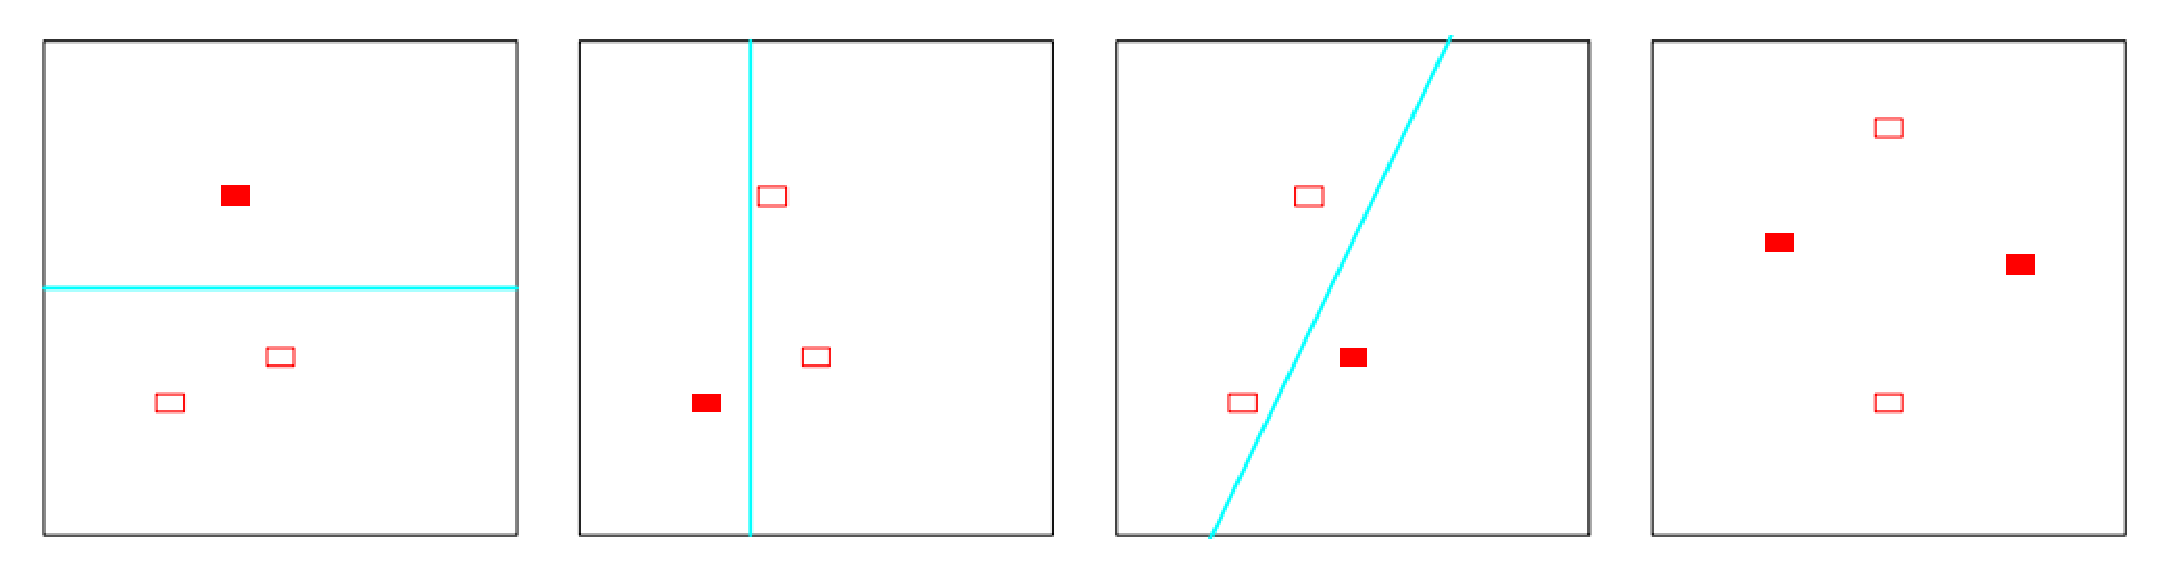
\includegraphics[width=0.85\textwidth]{figures/shatteredset.eps}
  \caption{二维空间线性模型的VC维}\label{fig:vcdimension}
\end{figure}
图例\ref{fig:vcdimension}左侧三个子图:对给定的三个点的点集,无论正负例如何分布,总存在线性模型可以将其精确地分开,线性分类模型可以将此点集碎化。对于四个点的点集,线性模型无法将右侧子图中分布的正负例精确分类,可以推断二维空间上的线性模型的VC 维等于3。根据生长函数可以推断得到相同的结论:对于图中三个点的点集,线性模型的生长函数为$s(\mathcal F,3) = 8 = 2^3$,而对于四个点的点集,生长函数为$s(\mathcal F,4) = 14 < 2^4$,故$V_{\mathcal F} = 3$。

目前尚无计算任意函数集VC维的通用理论,对于一些特殊的函数集,根据定义可以直接确定它们的VC维。比如,$n$维空间上的线性模型的VC维是$h=n+1$;正弦函数集$\{\sin(\omega x)\}$ 的VC 维是$h=\infty$。对于复杂的学习模型,比如人工神经网络,其VC维不仅与网络结构有关,还受学习算法的影响,因此其VC维的确定更加困难。通过理论或实验计算VC 维是目前统计学习理论有待研究的一个重要问题。

\begin{remark}
$\mathcal{F}$俨然是$S$的克星,纵然$S$有那八十二般变化,$\mathcal{F}$总有能人可以见招拆招,一准将其降住。正所谓,道高一尺魔高一丈,$S$ 唯有长叹:既生瑜何生亮,呜呼哀哉!$\mathcal{F}$的法术等级(VC维)可以根据其降服对手的最高等级(势)来确定:降服对手“势力”越强大,则其自身的等级越高。
\end{remark}

\section{期望风险与经验风险}
假设$X$是输入向量空间,$Y$是输出向量空间,乘积空间$Z=X\times Y$存在某种未知的概率分布$P(z) = P(x,y)$,统计学习的目标是从假设空间
$\mathcal F = \{f:X\rightarrow Y\}$中搜索一个最佳函数,使得\textbf{期望风险(Expected Risk)}:
\begin{equation}\label{eq:expectedrisk}
    R_{exp}(f) = \int_{X\times Y}{L(f(x),y)p(x,y)dxdy}
\end{equation}
最小,其中$L$表示损失函数。假设$\hat f$是假设空间中能够对概率分布$P(x,y)$做最佳逼近的函数,那么
\begin{equation}
    \hat f = \arginf\limits_{f\in \mathcal F}R_{exp}(f).
\end{equation}

由于概率分布$P(x,y)$未知,人们只能通过从未知分布中抽取样本集合$S=\{x_i,y_i\}_{i=1}^n$,间接估计出期望风险,这种风险损失又称为\textbf{经验风险}
(Empirical Risk):
\begin{equation}\label{eq:empiricalrisk}
    R_{emp}(f) = \frac{1}{n}\sum_i L(f(x_i),y_i)
\end{equation}
机器学习模型大多是基于经验风险最小化展开:
\begin{equation}\label{eq:slt-er}
    \hat f = \arginf\limits_{f\in \mathcal F} R_{emp}(f)
\end{equation}

通常,经验风险最小化的模型可能过于复杂,比如参数过多,从而产生过拟合问题,不利于模型泛化推广。模型过拟合是不稳定性的一种表现,训练数据集上的微小波动可能给最终训练得到的模型造成根本性的变化。研究表明,确保模型的稳定性,则模型的泛化能力与一致性也能得到保证。通过为经验风险增加一个正则化项,实际上限制了模型选择的范围,降低模型的复杂度,实现结构风险最小化的目的。正则化一般是在经验风险的基础上添加惩罚项:
\begin{equation}\label{eq:regularization}
    \min\limits_{f\in \mathcal F}\frac{1}{n}\sum\limits_i L(f(x_i),y_i) + \lambda \mathcal{R}(f)
\end{equation}
其中,$\mathcal{R}(f)$表示正则化项,$\lambda\ge 0$表示惩罚系数,反映对复杂模型选择的约束力度。

\section{泛化界}
统计学习理论系统地研究了经验风险$R_{emp}$(训练误差)和实际风险$R_{exp}$(期望风险)之间的关系,也即\textbf{泛化界}(Generalization Bound,也称“推广性的界”)。函数集$\mathcal F$的VC维反映了集合中函数的复杂程度,使用VC维可以确定函数$f$的泛化界。假设测试数据与训练数据独立同分布,$\mathcal{F}$ 是二元分类函数集,我们可以使用VC维预测二元分类模型$f\in \mathcal{F}$\textbf{测试误差的概率上界}:
\begin{equation}\label{eq:generalizationbound}
    P\bigg\{R_{exp}(f) \le R_{emp}(f) + \varPhi(n/h)\bigg\} \ge 1 - \eta.
\end{equation}
其中,$n$是训练样本容量,$h$表示函数集$\mathcal F$的VC维,
\[
    \varPhi(n/h) = \sqrt{\frac{h[\ln(2n/h) + 1] - \ln(\eta/4)}{n}}
\]
表示置信范围(或置信误差),$0<\eta<1$表示置信度。
%\begin{equation}\label{eq:testerrorupperbound}
%    R_{emp}(f) \le R_{exp}(f) \le R_{emp}(f) + \sqrt{\frac{h(\ln(2n/h) + 1) - \ln(\eta/4)}{n}} \triangleq  R_{emp}(f) + \varPhi(n/h)
%\end{equation}

如果训练样本有限,VC维$h$越大,则模型越复杂,并且置信范围$\varPhi(n/h)$越大,导致期望风险同经验风险之间的差别越大,从而产生常见的过拟合问题。在机器学习过程中,不仅要控制经验风险,还要控制VC维度以缩小置信范围,实现期望风险最小化,从而取得良好的泛化能力。当无法计算函数集的VC维时,可以采用交叉验证的方法,将样本集分为训练集和验证集,使用训练集样本训练模型,用验证集做测试,并选择验证集上误差最小的模型参数作为训练结果。

泛化界是基于最坏情况下的结论,多数情况下都是松弛的,并且不同模型泛化界的比较只有属于同一类函数集时才是有意义的。

\section{结构风险最小化}
传统的机器学习方法,选择以经验风险最小化作为目标,可能在训练集上可以达到100\%的准确率,但是泛化能力却很弱,执行预测时出现很高的误差。在选择学习模型与算法的过程是在调整置信范围,如果模型与训练样本匹配($h/n$恰当),则可能会取得不错的效果。模型的选择根据经验做出,过分倚重于“技巧”而缺乏理论指导。

统计学习理论给出一种具有指导性的策略:对函数集的子集,按照VC 维大小,即置信范围$\varPhi(h/n)$的大小顺次排列,构成一个函数子集序列:
\begin{equation}\label{eq:funtionalsubset}
    \begin{array}{l}
      \mathcal{F}_1 \subset \mathcal{F}_2 \subset \ldots \subset \mathcal{F}_m \\
      h_1 \le h_2 \le \ldots \le h_m
    \end{array}
\end{equation}
从函数子集中搜索能够最小化经验风险与置信范围之和的子集,实现最小化期望风险,这种思想称作\textbf{结构风险最小化}(Structural Risk Minimization),简称\textbf{SRM准则}。

实现SRM准则有两种思路:一是计算每个子集的最小经验风险,并从中选择经验风险与置信范围之和最小的子集。这种思路计算开销巨大,不可取。二是设计一种特殊的函数集结构,使得每个子集都能够取得最小的经验风险(训练误差为$0$),从中选择置信范围最小的子集。支持向量机正是第二种思想的实现。

%\subsection{Uniform Convergence Theory}

\section{支持向量机分类器}
对于一个包含$n$个样本的训练数据集\[S=\{x_i,y_i\}_{i=1}^n\]其中,$x_i\in \mathbb{R}^m$是样本特征向量,$y_i\in\{-1,1\}$是样本的类标。SVM模型就是求解下面的二次规划问题:
\begin{equation}\label{eq:svm}
    \begin{array}{ll}
      \min\limits_{\omega,b,\xi} & \frac{1}{2}\omega^T\omega + C\sum\limits_{i=1}^n\xi_i\\
      \textit{s.t.} & y_i(\omega^T\phi(x_i) + b) \ge 1 - \xi_i \\
      & \xi_i \ge 0 ,i = 1,2,\ldots,n
    \end{array}
\end{equation}
其中,样本$x_i$经由$\phi$映射到高维特征空间,$\omega$称作超平面法向量,$b$为超平面的截距,$\xi$表示松弛因子,$C >0$是$\ell_1$正则化项(Regularization Term)的惩罚系数。

引入拉格朗日乘子向量$\alpha,\beta \ge 0$,构造拉格朗日函数
\begin{equation}
    L(\omega,b,\xi,\alpha,\beta) = \frac{1}{2} \omega^T \omega + C\sum\limits_{i=1}^n\xi_i - \sum\limits_{i=1}^n \alpha_i \big[y_i(\omega^T\phi(x_i) + b) - 1 + \xi_i\big] - \sum\limits_{i=1}^n \beta_i \xi_i
\end{equation}
若记$\Theta_d(\alpha,\beta) = \min\limits_{\omega,b,\xi} L(\omega,b,\xi,\alpha,\beta)$,由于二次规划\eqref{eq:svm}具有强对偶性,存在全局最优解。一个解是最优解的充要条件是Karush-Kuhn-Tucker条件成立。根据KKT最优解的\textbf{平稳性条件}
\begin{equation}
    \left\{
    \begin{array}{l}
      \frac{\partial L}{\partial \omega} = \omega - \sum\limits_{i=1}^n \alpha_i y_i \phi(x_i) = 0 \\
      \frac{\partial L}{\partial b} = - \sum\limits_{i=1}^n \alpha_i y_i = 0 \\
      \frac{\partial L}{\partial \xi_i}  = C - \alpha_i - \beta_i = 0
    \end{array}
    \right.
\end{equation}
解得最优解$\hat \omega,\hat b,\hat \xi$:
\begin{equation}
    \left\{
    \begin{array}{l}
      \hat \omega = \sum\limits_{i=1}^n \alpha_i y_i \phi(x_i) \\
      \sum\limits_{i=1}^n \alpha_i y_i = 0 \\
      \alpha_i + \beta_i = C
    \end{array}
    \right.
\end{equation}
将其代入拉格朗日函数,整理后得:
\begin{equation}
    \Theta_d(\alpha,\beta) = L(\hat \omega,\hat b,\hat \xi,\alpha,\beta) = \sum\limits_{i=1}^n \alpha_i - \frac{1}{2} \sum\limits_{i=1}^n\sum\limits_{j=1}^n \alpha_i \alpha_j y_i y_j \phi(x_i)^T \phi(x_j)
\end{equation}
与$\beta$完全无关,根据$\alpha_i + \beta_i = C$,\textbf{对偶可行性条件}$\alpha_i\ge 0,\beta_i\ge 0$,可得下面形式的对偶模型:
\begin{equation}\label{eq:dualsvm}
    \begin{array}{ll}
      \max\limits_\alpha & \sum\limits_{i=1}^n \alpha_i - \frac{1}{2} \sum\limits_{i=1}^n \sum\limits_{j=1}^n \alpha_i \alpha_j y_i y_j \phi(x_i)^T \phi(x_j) \\
      \textit{s.t.} & \sum\limits_{i=1}^n \alpha_i y_i = 0 \\
      & 0\le \alpha_i \le C ,i = 1,\ldots,n
    \end{array}
\end{equation}
完全消除了松弛变量对模型的影响。假设对偶模型的最优解是$\hat \alpha,\hat \beta$,根据KKT最优解的\textbf{松弛互补条件}可得
\begin{equation}
    \left\{
    \begin{array}{l}
        \hat \alpha_i \big[y_i(\hat \omega^T \phi(x_i) + \hat b) - 1 + \hat \xi_i \big] = 0\\
        \hat \beta_i \hat \xi_i = 0
    \end{array}
    \right.
\end{equation}
对任意的$i = 1,\ldots,n$成立。由于$\hat \beta_i = C - \hat \alpha_i$
\begin{itemize}
  \item 当$\hat \alpha_i = 0$时,$\hat \beta_i = C$,则$\hat \xi_i=0$,$y_i(\hat \omega^T \phi(x_i) + \hat b) \ge 1$
  \item 当$0 < \hat \alpha_i < C$时,$\hat \beta_i>0$,则$\hat \xi_i=0$,$y_i(\hat \omega^T \phi(x_i) + \hat b) = 1$
  \item 当$\hat \alpha_i = C$时,$\hat \beta_i = 0$,则$\hat \xi_i = 1 - y_i(\hat \omega^T \phi(x_i) + \hat b) \ge 0$,$y_i(\hat \omega^T \phi(x_i) + \hat b) \le 1$
\end{itemize}

SVM从训练集中选择一组特征子集,使得对特征子集的划分等价于对整个数据集的划分,这组特征子集就被称为\textbf{支持向量}(Support Vector)。当$\hat \alpha_i=0$ 时,对应的样本数据是内部点,分类正确且远离最大间隔分类超平面;当$\hat \alpha_i=C$时,对应的样本数据可能分类错误;当$0< \hat \alpha_i < C$ 时,$y_i(\hat \omega^T \phi(x_i) + \hat b) = 1$ 对应的样本数据位于最大间隔边界上,属于支持向量。给定$\hat \alpha$利用$\hat \omega=\sum\limits_i \alpha_i y_i \phi(x_i)$ 可以计算最优的法向量$\hat \alpha$ 与截距$\hat b$。根据SVM 模型在训练数据集上训练出一个最佳超平面分类模型:
\begin{equation}\label{eq:hyperplane}
    f(x) = \sgn(\hat \omega^T \phi(x) + \hat b) = \sgn(\sum_i \hat \alpha_i y_i \phi(x_i)^T \phi(x) + \hat b)
\end{equation}
对于部分$\hat \alpha_i = C$的样本可能分类错误,可应用于异常点检测问题\cite{matic1992computer}。

最大化分类间隔是控制泛化能力的一个举措,也是SVM的一个核心思想。根据统计学习理论\cite{vapnik1982estimation,vapnik2000nature},在$m$维空间中,如果所有样本都分布在半径为$r$的超球内,则满足条件$\|\omega\| \le z$的指示函数集$f(\omega, b) = \sgn(\omega^T x + b)$的VC维$h$有如下上界:
\begin{equation}
    h \le \min~\{\lceil r^2 z^2\rceil, m\} + 1
\end{equation}
实际上最小化$\|\omega\|^2$的目标体现了最小化VC维上界的SRM准则,有利于选择一个泛化能力强的模型。

\section{核方法}
1964年Aizermann等人~\cite{aizerman1964theoretical}在研究势函数方法时最先使用核方法,1992年Vapnik等人~\cite{boser1992training}同时利用核函数与最大间隔超平面,基于结构风险最小化原理提出SVM。核方法是SVM 成功的关键,赋予SVM处理非线性问题的能力。在具体问题中,选择合适的核函数仍然存在许多实际困难。

\begin{definition}[Gram矩阵]
假设$K(x,y)$是$X\times X$上的一个对称函数,对于输入空间$X$上的一组向量$x_1,\ldots,x_n$,则称矩阵$(K(x_i,x_j))_{n\times n}$为函数$K(x,y)$关于向量组$x_1,\ldots,x_n$的Gram矩阵。
\end{definition}

\begin{definition}[核函数与核矩阵]
给定输入空间$X$,对称函数$K:X\times X\mapsto \mathbb R$,如果存在一个希尔伯特特征空间$H$,及$X$到$H$的映射
\begin{equation}
    \phi: X \mapsto H
\end{equation}
使得任意$x,y\in X$,都有
\begin{equation}
    K(x,y) = \phi(x)^T \phi(y)
\end{equation}
则称$K(x,y)$是$X\times X$上的一个\textbf{核函数},$\phi(x)$为映射函数。对于$X$上的一组向量$x_1,\ldots,x_n$,核函数$K(x,y)$ 关于向量组$x_1,\ldots,x_n$的Gram矩阵
\begin{equation}
    K =
    \begin{bmatrix}
    K_{11}& K_{12} & \cdots & K_{1n}\\
    K_{21}& K_{22} & \cdots & K_{2n}\\
    \vdots & \vdots & \ddots & \vdots\\
    K_{n1}& K_{n2} & \cdots & K_{nn}\\
    \end{bmatrix}
\end{equation}
称作\textbf{核矩阵},其中$K_{ij}=K(x_i, x_j)$。
\end{definition}
对于给定的核函数$K(x,y)$,特征空间$H$和映射函数$\phi$的选取并不唯一,可以取不同的特征空间,即便是在同一个特征空间上也可以取不同的映射。通过核函数构造映射函数通常比较复杂,研究人员提出一个重要的问题:不用构造映射函数$\phi(x)$,能否直接判断一个给定的函数$K(x,y)$是不是核函数?换而言之,函数$K(x,y)$满足什么条件时才能成为核函数?

\begin{theorem}[Mercer条件\cite{mercer1909functions}]
对称函数$K:X\times X\mapsto \mathbb{R}$为正定核(或Mercer 核),当且仅当它关于$X$上任意一组向量$x_1,\ldots,x_n$的Gram矩阵$K = [K(x_i,x_j)]_{n\times n}$ 都是半正定(Positive Semi-definitive)矩阵。
\end{theorem}
\begin{proof}
\textbf{必要性}:若$K(x,y)$是$X\times X$上的正定核,则存在映射$\phi:X\mapsto H$,使得
\[
    K(x,y) = \phi(x)^T \phi(y), \forall x,y\in X,
\]
那么,对于任意一组$X$上的向量$x_1,\ldots,x_n$,我们可以根据正定核$K(x,y)$构造对应的Gram矩阵$K=[K_{ij}]_{n\times n} = [K(x_i,x_j)]_{n\times n}$,对任意的$c_i\in \mathbb{R},i=1,\ldots,n$,都有
\begin{equation}
    \sum\limits_{i,j} c_i c_j K(x_i,x_j) = \sum\limits_{i,j} c_i c_j \phi(x)^T \phi(y) = [\sum\limits_i c_i \phi(x_i)]^T[\sum\limits_j c_j\phi(x_j)] = \|\sum\limits_i c_i \phi(x_i)\|^2 \ge 0
\end{equation}
表明核矩阵都是半正定矩阵。

\textbf{充分性}:对于任意的$x_i\in X,i=1,\ldots,n$,函数$K(x,y)$关于$x_1,\ldots,x_n$的Gram 矩阵$K = [K(x_i,x_j)]_{n\times n}$是半正定矩阵。我们使用构造性证明方法,通过三个步骤在函数$K(x,y)$的基础上构造出一个希尔伯特空间$H$、输入空间$X$到希尔伯特空间$H$的一个映射$\phi$:

\noindent \textbf{1、向量空间}:
定义映射$\phi:x\mapsto K(\cdot,x)$,则对任意$x_i\in X,\alpha_i\in \mathbb{R},i=1,\ldots,n$,可以定义线性组合
\begin{equation}
    f(\cdot)=\sum\limits_{i=1}^n \alpha_i K(\cdot,x_i)
\end{equation}
构成集合$S$。由于集合$S$对加法和数乘运算封闭,因此构成向量空间。

\noindent \textbf{2、内积空间}:
对$S$上的任意两个元素
\[
    f(\cdot)=\sum\limits_{i=1}^n \alpha_i K(\cdot,x_i), ~~g(\cdot)=\sum\limits_{j=1}^m \beta_j K(\cdot,y_j)
\]
定义一个二元运算$\times$:
\[
    f\times g = \sum\limits_{i=1}^n \sum\limits_{j=1}^m \alpha_i \beta_j K(x_i,y_j)
\]
可以证明运算$\times$是空间$S$的内积,满足如下五个性质:
\begin{eqnarray}
  (cf)\times g = c(f\times g), \\
  (f+g)\times h = f\times h + g\times h, \\
  f \times g = g\times f, \\
  f\times f \ge 0, \\
  f\times f = 0 \Leftrightarrow f = 0.
\end{eqnarray}
根据函数$K(x,y)$的对称性,容易证明前三个等式。由于
\[
    f\times f = \sum\limits_{i=1}^n \sum\limits_{j=1}^n \alpha_i \alpha_j K(x_i,x_j)
\]
根据Gram矩阵的半正定性可知等式右端非负,从而可证$f\times f\ge 0$。 对于最后一个命题,充分性显然,下面证明必要性。

由于$S$是向量空间,则对任意的$\lambda\in \mathbb{R}$,若$f,g\in S$,则$f + \lambda g\in S$。根据$(f + \lambda g) \times (f + \lambda g) \ge 0$,展开可以得到一个关于$\lambda$ 的二次函数
\[
  f\times f + 2\lambda f\times g + \lambda^2 g\times g \ge 0
\]
由$\lambda$的任意性知
\[(f\times g)^2 \le (f\times f)(g\times g).\]
根据运算$\times$的定义,对任意的$x\in X$都有
\[K(\cdot,x) \times f = \sum\limits_{i=1}^m \alpha_i K(x,x_i) = f(x),\]
从而有
\[f(x)^2 = (K(\cdot,x) \times f)^2 \le [K(\cdot,x) \times K(\cdot,x)](f\times f).\]
如果$f\times f = 0$,则对任意的$x\in X$,都有$f(x)=0$,那么$f=0$。由此可以证明$\times$是向量空间$S$的内积,$S$为一个内积空间。为表述方便,我们统一记
\[f^T g=f\times g = \sum\limits_{i=1}^n \sum\limits_{j=1}^m \alpha_i \beta_j K(x_i,y_j).\]

\noindent \textbf{3、完备的内积空间——希尔伯特空间}:
根据内积空间$S$定义的内积运算可以自然地诱导出范数
\[
    \|f\| = (f^T f)^{1/2}
\]
因此内积空间$S$也是一个赋范空间。根据泛函分析理论,对于不完备的内积空间$S$,一定可以完备化成为希尔伯特空间(完备的内积空间)$H$。对于给定的函数$K(x,y)$,可以构造从$X$到某个希尔伯特空间$H$的映射$\phi:x\mapsto K(\cdot,x)$,并且满足
\[
    K(\cdot,x)^T f=f(x),\qquad K(\cdot,x)^T K(\cdot,y) = K(x,y)
\]
则根据映射定义可知$K(x,y)=\phi(x)^T \phi(y)$,表明$K(x,y)$是$X\times X$上的核函数。
\end{proof}

\begin{definition}[正定核]
如果对称函数$K(x,y)$关于$x_i\in X,i=1,\ldots,n$的Gram矩阵是半正定矩阵,则称它是正定核。
\end{definition}

\begin{corollary}
正定核的非负线性组合仍然是正定核。
\end{corollary}

\begin{definition}[再生核希尔伯特空间]
假设$H$是由函数$f:X\mapsto \mathbb{R}$构成的希尔伯特空间,如果函数$K: X\times X \mapsto \mathbb R$满足\textbf{再生性},对任意$x\in X$都有$K(\cdot,x)\in H$,且对任意$f\in H$都有
\begin{equation}
    f(x) = K(\cdot,x)^T f
\end{equation}
则称$K$是$H$的\textbf{再生核}。如果$H=\overline{span\{K(\cdot,x),x\in X\}}$(或Dirac泛函$\delta_x(f)=f(x)$连续),$\bar A$ 表示集合$A$ 的闭包,则称空间$H$是\textbf{再生核希尔伯特空间}(Reproducing Kernel Hilbert Space, RKHS)。
\end{definition}

\begin{theorem}[表示定理]
Tikhonov正则化问题
\begin{equation}
    \min\limits_{f\in H}~\frac{1}{2} \sum\limits_{i=1}^n L(f(x_i),y) + \frac{1}{2} \lambda\|f\|_K^2
\end{equation}
的解可以写作
\begin{equation}
    f = \sum\limits_{i=1}^n \alpha_i K(\cdot,x_i)
\end{equation}
的形式。其中,$L(\cdot,\cdot)$是损失函数,$\|\cdot\|_K^2$是正则化项,同输入空间$X\times X$上的核函数$K(\cdot,\cdot)$有关。
\end{theorem}

假设核函数$K(x,y)$关于$\{x_1,x_2,\ldots,x_n\}$生成的核矩阵为$K = K^T$,根据表示定理,任选一个向量$x_j$,都有
\begin{equation}
    f(x_j)=\sum\limits_{i=1}^n \alpha_i K(x_i,x_j)=\alpha^T K_j.
\end{equation}
其中,$K_j$表示矩阵$K$的第$j$ 列。由内积定义,我们可以推断知
\begin{equation}
    \|f\|_K^2 = [\sum\limits_{i=1}^n \alpha_i K(\cdot,x_i)]^T [\sum\limits_{i=1}^n \alpha_i K(\cdot,x_i)] = \sum\limits_{i=1}^n \sum\limits_{j=1}^n \alpha_i\alpha_j K(x_i,x_j) = \alpha^T K \alpha.
\end{equation}
如果假设损失函数$L$为平方差损失,则原始Tikhonov正则化问题可等价地写作
\begin{equation}
    \min\limits_{\alpha\in\mathbb{R}^n}~\frac{1}{2} \|K \alpha - y\|^2 + \frac{1}{2} \lambda \alpha^T K \alpha,
\end{equation}
根据极值必要性条件有解
\begin{equation}
    \alpha = (K  + \lambda I)^{-1} y.
\end{equation}
只要正则化因子$\lambda$选择恰当,就可以保证$K + \lambda I$的非奇异/正定性。当使用线性核$K(x,y)=x^T y$时,则$K = X^T X$,问题就转化为岭回归问题:
\begin{equation}
    \alpha = (X^T X  + \lambda I)^{-1} y
\end{equation}
Tikhonov正则化方法有助于控制模型的平滑性,避免欠拟合与过拟合问题。

在机器学习领域,常用的核函数有如下几种:
\begin{enumerate}[(1)]
  \item 线性核函数(Linear Kernel):$K(x,y) = x^T y$
  \item 多项式核函数(Polynomial Kernel):$K(x,y) = (\gamma x^T y + r)^d$
  \item 高斯径向基函数(Gaussian Radial Basis Function, RBF):$K(x,y) = e^{-\|x - y\|^2/2\gamma^2}$
  \item Sigmoid核函数:$K(x,y) = \tanh\{-\gamma x^T y + r\}$
  \footnote{$\tanh x = \frac{e^x - e^{-x}}{e^x + e^{-x}}$}
\end{enumerate}
根据核函数的性质,我们还可以组合多个核函数构成复杂的核函数。

利用标准二次优化技术训练SVM模型有诸多不便,存在模型复杂不易实现、核矩阵的存储与计算开销大、训练速度慢等问题。为了解决训练速度问题,人们提出很多改进算法,包括块算法(Chunking Algorithm)\cite{vapnik1982estimation}、Osuna算法\cite{osuna1997improved}、SMO算法\cite{platt1998sequential}、SVMLight算法
\cite{joachims1999making,joachims2002learning}、Pegasos算法\cite{shalev2007pegasos} 等。

\section{块算法}
由于支持向量机分类模型只与支持向量有关,同其他所有训练样本都无关,如果仅使用支持向量作为训练集,可以训练得到一致的分类模型。1982年,Vladimir Vapnik与Samuel Kotz根据这种思想提出了块算法(Chunking Algorithm)\cite{vapnik1982estimation}。块算法将训练数据集分成两部分:工作样本集与测试样本集,在工作样本集上应用二次规划优化算法,得到由支持向量表示的分类模型,再利用它从余下所有样本中筛选出违反KKT条件的样本,并入支持向量构成新的工作样本集,然后重新训练。根据这种分解策略,如果样本中支持向量数目很少,工作集样本的数目远小于总样本个数,则可以节省大量的训练时间。在实际应用中,支持向量的数目可能很多,随着迭代的不断推进,工作样本集的规模将逐渐扩大,增加了训练的负担。

\section{Osuna分解算法}
1997年,Edgar Osuna等人\cite{osuna1997support,osuna1997improved}提出Osuna分解算法,在每次迭代训练时固定工作样本集(工作集,Working Set)的规模,将非工作集上违反KKT 条件最严重的样本与工作样本集中的样本进行等量交换,无论支持向量数目多大,都不会改变工作样本集的规模。由于Osuna算法涉及到一个工作样本换出问题,换出的工作样本可能是一个支持向量,那么此算法的关键就在于选择一种合适的样本换入换出策略,确保算法能够收敛并且快速地收敛到最优结果。

Osuna算法固定工作集的规模,并假设其规模足以包含所有的支持向量($\alpha_i>0$),同时又不会超出计算机解决子问题的能力范围(内存、计算复杂度)。它将数据集分解成两部分:工作集B与非工作集N,相应地乘子集也分成两部分,保持非工作集对应的乘子不变,在工作集上定义下面形式的子问题:
\begin{equation}
    \begin{array}{ll}
      \max\limits_{\alpha_B} & \Theta(\alpha_B,\alpha_N)\\
      \textit{s.t.} & \sum\limits_{i\in B} \alpha_i y_i + \sum\limits_{i\in N} \alpha_i y_i = 0 \\
      & 0\le \alpha_i \le C ,i\in B
    \end{array}
\end{equation}
根据工作集B与非工作集N,原问题的目标函数可以表示成下面的形式:
\begin{eqnarray}
    \Theta(\alpha_B,\alpha_N) &=&\big[\sum\limits_{i\in B} \alpha_i - \frac{1}{2} \sum\limits_{i\in B} \sum\limits_{j\in B} \alpha_i\alpha_j y_i y_j K_{ij} - \sum\limits_{i\in B}\sum\limits_{j\in N} \alpha_i\alpha_j y_i y_j K_{ij}\big] + \\
   && \big[\sum\limits_{i\in N} \alpha_i - \frac{1}{2} \sum\limits_{i\in N} \sum\limits_{j\in N} \alpha_i\alpha_j y_i y_j K_{ij}\big].
\end{eqnarray}
在子问题中,$\alpha_B$是所有工作集对应乘子构成的列向量,非工作集N上的乘子保持固定为常数,子问题的目标函数可以将其忽略。子问题的规模与非工作集的大小、支持向量的数目无关。

\begin{theorem}[Osuna定理]
如果从工作集B中换出一个变量到非工作集N,则原问题的目标函数值不变,原问题的新解也是子问题的可行解。如果非工作集N中存在一个违反KKT条件的变量,将其换入到工作集B,则重新优化子问题后,原问题的目标函数值严格递增。
\end{theorem}
\begin{proof}
假设从工作集B中换出的样本为$x_v$,则新工作集为$B'=B\setminus \{v\}$,新的非工作集为$N'=N\cup\{v\}$,则有
\begin{equation}
    \begin{array}{ll}
       & \Theta(\alpha_B,\alpha_N) \\
      = & \sum\limits_{i\in B} \alpha_i - \frac{1}{2} \sum\limits_{i\in B} \sum\limits_{j\in B} \alpha_i\alpha_j y_i y_j K_{ij} - \sum\limits_{i\in B}\sum\limits_{j\in N} \alpha_i\alpha_j y_i y_j K_{ij} + \sum\limits_{i\in N} \alpha_i - \frac{1}{2} \sum\limits_{i\in N} \sum\limits_{j\in N} \alpha_i\alpha_j y_i y_j K_{ij}\\
      = & \sum\limits_{i\in B'} \alpha_i - \frac{1}{2} \sum\limits_{i\in B'} \sum\limits_{j\in B'} \alpha_i\alpha_j y_i y_j K_{ij} - \sum\limits_{i\in B'}\sum\limits_{j\in N'} \alpha_i\alpha_j y_i y_j K_{ij} + \sum\limits_{i\in N'} \alpha_i - \frac{1}{2} \sum\limits_{i\in N'} \sum\limits_{j\in N'} \alpha_i\alpha_j y_i y_j K_{ij} \\
      = & \Theta(\alpha_{B'},\alpha_{N'})
    \end{array}
\end{equation}
表明原问题目标函数值不变。对于原问题的新解$(\alpha_{B'},\alpha_{N'})$,满足子问题的等式约束
\begin{equation}
    \sum\limits_{i\in B'} \alpha_i y_i + \sum\limits_{i\in N'} \alpha_i y_i = \sum\limits_{i\in B} \alpha_i y_i + \sum\limits_{i\in N} \alpha_i y_i = 0
\end{equation}
且满足子问题的不等式约束,则新解$\alpha_{B'}$也是子问题的可行解。对于反向操作,我们可以得到相同的结论。

对于非工作集N,如果存在违反KKT条件的样本$x_u$,则它必然满足如下某个条件:
  \begin{equation}
    \left\{
    \begin{array}{ll}
        \alpha_u=0, & y_u [\omega_u^T \phi(x_u) + b] < 1\\
        0<\alpha_u<C, & y_u [\omega_u^T \phi(x_u) + b] \ne 1\\
        \alpha_u=C, & y_u [\omega_u^T \phi(x_u) + b] > 1
    \end{array}
    \right.
  \end{equation}
将其换入到工作集B,显然不会改变原问题的目标函数值,并且原问题的新解对于新的子问题可行。对于工作集$B'$上新的子问题
  \begin{equation}
    \begin{array}{ll}
      \max\limits_{\alpha_{B'}} & \Theta(\alpha_{B'},\alpha_{N'})\\
      \textit{s.t.} & \sum\limits_{i\in B'} \alpha_i y_i + \sum\limits_{i\in N'} \alpha_i y_i = 0 \\
      & 0\le \alpha_i \le C ,i\in B'
    \end{array}
  \end{equation}
经过优化求解以后,必然有
\begin{equation}
    \Theta(\alpha_B,\alpha_N) = \Theta(\alpha_{B'},\alpha_{N'}) \le \max\limits_{\alpha_{B'}}~\Theta(\alpha_{B'},\alpha_{N'})
\end{equation}
能够逐步改善原问题的目标函数值。
\end{proof}

Osuna算法将原问题分解为一系列子问题,通过求解所有子问题实现求解原问题的目的,它包括三个基本步骤:
\begin{itemize}
  \item 从数据集中任意固定数目的样本构成工作集B
  \item 优化求解定义在工作集B上的子问题
  \item 对于非工作集,如果存在违反KKT条件的样本$x_j$,从工作集B中任选一个样本$x_i$与之交换,并优化求解新工作集$B'=B\setminus\{x_i\}\cup\{x_j\}$ 上的子问题
\end{itemize}

由于原问题与子问题都具有凸可行域,并且目标函数为凸二次函数,则目标函数有界,Osuna算法一定可以在有限次迭代后收敛到全局最优解。Osuna算法与块算法的主要区别在于目标函数的构成,Osuna算法包含全部训练样本(工作集与非工作集),目标函数在保持上次迭代结果的基础上,优化新工作集上定义的子问题。块算法每次迭代直接设定工作集以外的拉格朗日乘子为零,收敛效率低且目标函数值并非最优。

\section{序列最小优化算法}
1998年,微软研究院的John Platt\cite{platt1998sequential}提出著名的\textbf{序列最小优化算法}(Sequential Minimal Optimization,简称SMO),可以高效地训练线性SVM模型,易于实现和扩展,尤其适合处理大型稀疏数据。SMO算法吸收Osuna算法的分治思想,\textbf{将二次规划问题分解成一系列存在解析解的最小子问题},通过子问题实现求解原始凸优化问题。2001年,Chih-Jen Lin\cite{lin2001convergence}给出SMO算法严格的收敛性证明。

如果我们将正定核$K(x,y)$引入到模型\eqref{eq:dualsvm},可以得到下面形式的凸优化问题:
\begin{equation}
    \begin{array}{ll}
      \max\limits_\alpha & \Theta(\alpha) = \sum\limits_{i=1}^n \alpha_i - \frac{1}{2} \sum\limits_{i=1}^n \sum\limits_{j=1}^n \alpha_i \alpha_j y_i y_j K_{ij} \\
      \textit{s.t.} & \sum\limits_{i=1}^n \alpha_i y_i = 0 \\
      & 0\le \alpha_i \le C ,i = 1,\ldots,n
    \end{array}
\end{equation}
每个拉格朗日乘子都对应一个训练样本,模型中的不等式约束条件构成典型的凸包。SMO算法与Osuna算法类似,将原始数据集分解成两部分:工作集与非工作集,并且固定工作集的规模至最小。当工作集降至只有一个变量时,根据等式约束条件,工作集对应的乘子变量直接固定,无法实现优化子问题目标函数的目的。SMO算法将工作集固定为两个变量($|B|=2$),根据等式约束与变量界的不等式约束,可以直接通过解析式优化子问题的目标函数。

\subsection{解析方法:优化拉格朗日乘子对}
假定当前满足全部约束条件的拉格朗日乘子向量$\alpha^t$,根据Osuna算法(或坐标上升法)的思想,我们选定工作集为$B=\{i,j\}$。不失一般性,假设$i<j$,则非工作集为$N=\{1,2,\ldots,i-1, i+1,\ldots,j-1,j+1,\ldots,n\}$。在下次迭代时,SMO算法保持非工作集当前状态不变,则目标函数变成一个形式简单的二元二次函数:
\begin{equation}
    \begin{array}{lll}
    \Theta(\alpha) & = & \Theta(\alpha_1^t,\ldots, \alpha_{i-1}^t, \textcolor{red}{\alpha_i},\alpha_{i+1}^t,\ldots,\alpha_{j-1}^t,\textcolor{red}{\alpha_j},\alpha_{j+1}^t,\ldots,\alpha_n^t) \\
    & = & \alpha_i \big[ 1 - y_i \sum\limits_{k\in N} \alpha_k^t y_k K_{ik} \big] + \alpha_j \big[1 - y_j \sum\limits_{k\in N} \alpha_k^t y_k K_{jk}\big]\\
    && - \alpha_i \alpha_j y_i y_j K_{ij} - \frac{1}{2} \alpha_i^2 K_{ii} - \frac{1}{2} \alpha_j^2 K_{jj} + \Theta_N
    \end{array}
\end{equation}
其中$\Theta_N$是只与非工作集N有关,但与$\alpha_i,\alpha_j$无关的常量。根据问题的约束条件,可行域被限定在矩形区域$[0,C]\times[0,C]$ 内的线段上
\begin{equation}
    \alpha_i y_i + \alpha_j y_j = -\sum\limits_{k\in N} \alpha_k^t y_k = \alpha_i^t y_i + \alpha_j^t y_j
\end{equation}
等式两端同时乘以$y_j$可得
\begin{equation}
    \alpha_j = \alpha_j^t + y_i y_j (\alpha_i^t - \alpha_i).
\end{equation}
我们由此将原始的二元目标函数化为一元二次函数,从而获取解析形式的最优解。根据工作集中两个变量的线性关系,以及变量的边界条件
\begin{equation}
    \left\{
    \begin{array}{c}
      0\le \alpha_i \le C \\
      0\le \alpha_j \le C
    \end{array}
    \right.
\end{equation}
可以确定变量$\alpha_j$的范围$[L, H]$:
\begin{itemize}
  \item 当$y_i y_j = 1$时,$\alpha_j = \alpha_j^t + \alpha_i^t - \alpha_i$,则有
      \begin{equation}
        L = \max\{0,\alpha_i^t + \alpha_j^t - C\},\quad H = \min\{C,\alpha_i^t + \alpha_j^t\}
      \end{equation}
  \item 当$y_i y_j = -1$时,$\alpha_j = \alpha_j^t - \alpha_i^t + \alpha_i$,则有
      \begin{equation}
        L = \max\{0,\alpha_j^t - \alpha_i^t\},\quad H = \min\{C,\alpha_j^t-\alpha_i^t+C\}
      \end{equation}
\end{itemize}

\noindent 对于单变量函数,根据极值必要性条件,令一阶导函数$\nabla_j \Theta(\alpha) = 0$,可以算得$\Theta(\alpha)$的无约束最优解
\begin{equation}
    \hat\alpha_j = \alpha_j^t + \frac{y_j(e_i - e_j)}{K_{ii} + K_{jj} - 2 K_{ij}}.
\end{equation}

它由两部分构成,第一部分为上次迭代结果,第二部分
\begin{equation}\label{eq:updatestep}
    \Delta_j = \frac{y_j (e_i - e_j)}{K_{ii} + K_{jj} - 2 K_{ij}}
\end{equation}
可以视为变量$\alpha_j$更新的步长,其中
\begin{equation}
    e_k = \big[\sum\limits_{l=1}^n y_l \alpha_l^t K_{kl} + b\big] - y_k, \quad k = i, j
\end{equation}
表示模型的预测误差。从目标函数的凹凸性来看,一般地都有
\begin{equation}
    \nabla^2_{jj} \Theta(\alpha) = 2 K_{ij} - K_{ii} - K_{jj}  = -\|\phi(x_i) - \phi(x_j)\|^2 < 0,
\end{equation}
表明目标函数在$(-\infty, \hat\alpha_j)$范围单调递增,在$(\hat\alpha_j,\infty)$范围单调递减。由于可行域在$[L,H]$,则$\hat\alpha_j$未必是可行解。为确保目标函数的最优解可行,我们在边界$L$与$H$处作如下处理
\begin{equation}
    \alpha_j^{t+1} = \left\{
    \begin{array}{ll}
      H, & \hat\alpha_j  > H \\
      \hat\alpha_j,  & L \le \hat\alpha_j  \le H \\
      L, & \hat\alpha_j < L
    \end{array}
    \right.
\end{equation}
根据$\alpha_i$与$\alpha_j$的关系可以根据下式更新$\alpha_i^t$
\begin{equation}
    \alpha_i^{t+1} = \alpha_i^t + y_i y_j (\alpha_j^t - \alpha_j^{t+1}).
\end{equation}

如果如果核函数不满足Mercer条件,则可能导致$\eta_{ij} = 2K_{ij} - K_{ii} - K_{jj} >0$。如果数据集中存在多个相同的输入样本,可能出现$\eta_{ij}=0$。 当$\eta_{ij}\ge 0$ 时,需要在可行域线段上逐个验证,确定能够给目标函数带来最大提升的位置。

\textbf{如果$\hat\alpha_j$是可行解,那么可以保证目标函数在更新后有所改善。如果$\hat\alpha_j$不可行,根据边界确定的可行解可能无法保证目标函数的改善,若没有改善,则恢复到上次迭代的结果,重新选择新的工作集,确保目标函数随迭代次数的增加单调递增。}

\subsection{启发式方法:选取拉格朗日乘子对}
根据Osuna定理\cite{osuna1997improved},SMO算法只要在每一步迭代都能够选择优化两个工作样本,在优化前工作集至少包含一个违反KKT条件的样本,就可以保证目标函数稳步提升。算法的收敛性也可以得到保证。为了提高收敛的速度,SMO算法使用启发式的方式选择并联合优化两个工作样本$\alpha_i$与$\alpha_j$:遍历整个样本空间,选出在一定阈值范围$\epsilon>0$内违反KKT条件的样本作为第一个工作样本$\alpha_i$;遍历所有的非边界数据集,选择出最大化更新步长的样本作为第二个工作样本$\alpha_j$(如果非边界数据集为空,则随机选择一个不同于$\alpha_i$的工作样本)。选择$\alpha_i$的工作计算密集,主要开销集中在对样本,尤其是非边界样本上的KKT 条件检验。

KKT条件是凸优化问题收敛的充要条件,当所有样本都满足KKT条件时,就说明算法已经收敛,从而可以终止迭代。在具体实现时,对KKT 条件的检验都存在一定范围的误差$\epsilon>0$,只要样本在阈值范围内满足KKT条件,都认定是样本满足KKT条件。此外,我们通过分析原问题与对偶问题的对偶间隙,可以发现KKT条件的判定法则与最小化对偶间隙优化目标的一致性。

假设原问题的最优目标函数值为$p$,对偶问题的最优目标函数值为$d$,人们称两者之间的差为对偶间隙
\begin{equation}
    \begin{array}{lll}
      \delta & = & p - d \\
       & = & \big(\frac{1}{2} \omega^T \omega + C\sum\limits_{i=1}^n \xi_i\big) - \big(\sum\limits_{i=1}^n \alpha_i - \frac{1}{2} \sum\limits_{i=1}^n \sum\limits_{j=1}^n \alpha_i \alpha_j y_i y_j K_{ij}\big)  \\
       & = & \sum\limits_{i=1}^n \sum\limits_{j=1}^n \alpha_i \alpha_j y_i y_j K_{ij} - \sum\limits_{i=1}^n \alpha_i + C\sum\limits_{i=1}^n \xi_i \\
    \end{array}
\end{equation}
对于任意一个样本$x_i$,我们从对偶间隙中分解出它的贡献
\begin{equation}
    \delta_i = \alpha_i y_i \sum\limits_{j=1}^n \alpha_j y_j K_{ij} - \alpha_i + C\xi_i = \alpha_i (y_i g_i - 1 - y_i b) + C\xi_i
\end{equation}
其中,$g_i = \sum\limits_{j=1}^n \alpha_j y_j K_{ij} + b$。根据KKT条件可知:
\begin{itemize}
  \item 当$\alpha_i = 0$时,$y_i g_i \ge 1$($\xi_i=0$),则$\delta_i =  0$
  \item 当$0 < \alpha_i < C$时,$y_i g_i = 1$($\xi_i=0$),则$\delta_i = \alpha_i (y_i g_i - 1 - y_i b)= - \alpha_i b y_i$
  \item 当$\alpha_i = C$时,$y_i g_i \le 1$($\xi_i = 1 - y_i g_i \ge 0$),则$\delta_i = - b C y_i$
\end{itemize}
其中$0<\alpha_i<C$对应的样本称作\textbf{非边界数据点(Non-bound)},如果样本$x_i$违反了KKT条件:
\begin{itemize}
  \item 当$\alpha_i = 0$时,$y_i g_i < 1$($\xi_i> 0$),则$\delta_i = C\xi_i >0$
  \item 当$0 < \alpha_i < C$时,$y_i g_i > 1$($\xi_i=0$),则$\delta_i = \alpha_i (y_i g_i - 1 - y_i b) > - \alpha_i b y_i$
  \item 当$0 < \alpha_i < C$时,$y_i g_i < 1$($\xi_i= 1 - y_i g_i>0$),则$\delta_i = (C-\alpha_i)(1 - y_i g_i)-\alpha_i b y_i > - \alpha_i b y_i$
  \item 当$\alpha_i = C$时,$y_i g_i > 1$($\xi_i=0$),则$\delta_i = - b C y_i + C (y_i g_i - 1)>- b C y_i $
\end{itemize}
数据集中违反KKT条件的样本,会增大对偶间隙,进而影响到优化算法的收敛速度。在所有的数据样本中,非边界数据点违反KKT条件的可能性最大,为此SMO算法从第二次迭代开始,在选择第一个工作样本时,首先检测非边界数据集是否满足收敛条件。如果所有非边界数据均满足KKT条件,则算法再检测整个数据集以确保所有样本均满足收敛条件。

SMO算法使用启发式的方法选择第一个优化变量$\alpha_i$后,在筛选第二个优化变量$\alpha_j$时,选择的标准是希望$\alpha_j$发生足够大的变化。根据
\eqref{eq:updatestep}可知:
\begin{equation}
    \alpha_j = \argmax\limits_{k\ne i} |\Delta_k| = \argmax\limits_{k\ne i} \frac{|e_i - e_k|}{|\eta_{ik}|}
\end{equation}
由于$|\eta_{ik}|$牵涉到核矩阵的计算,时间开销较大,为此我们近似地选择优化$|e_i - e_k|$,即
\begin{equation}
    \alpha_j = \argmax\limits_{k\ne i} |e_i - e_k|
\end{equation}

\subsection{确定截距}
每次迭代都要重新计算截距$b$,保证$x_i,x_j$满足KKT条件。当$\alpha_i^{t+1}$在界内,即$0<\alpha_i^{t+1}<C$时,则根据KKT条件应当有$y_i g_i^{t+1} = 1$,两边同时乘以$y_i$,整理可得:
\begin{equation}
    \begin{array}{lll}
        y_i & = & g_i^{t+1} \\
            & = & \sum\limits_{k=1}^n \alpha_k^{t+1} y_k K_{ik} + b^{t+1} \\
            & = & \alpha_i^{t+1} y_i K_{ii} + \alpha_j^{t+1} y_j K_{ij} + \sum\limits_{k\in N} \alpha_k^t y_k K_{ik} + b^{t+1}
    \end{array}
\end{equation}
经过$t$次迭代后,模型在$x_i$上的预测误差为
\begin{equation}
    e_i^t = g_i^t - y_i = \alpha_i^t y_i K_{ii} + \alpha_j^t y_j K_{ij} + \sum\limits_{k\in N} \alpha_k^t y_k K_{ik} + b^t - y_i
\end{equation}
从而可以确立截距的更新规则:
\begin{equation}
    b^{t+1} = b^t - e_i^t - (\alpha_i^{t+1} - \alpha_i^t) y_i K_{ii} - (\alpha_j^{t+1} - \alpha_j^t) y_j K_{ij}
\end{equation}
类似地,对于处于界内的$\alpha_j^{t+1}$同样有
\begin{equation}
    b^{t+1} = b^t - e_j^t - (\alpha_i^{t+1} - \alpha_i^t) y_i K_{ij} - (\alpha_j^{t+1} - \alpha_j^t) y_j K_{jj}
\end{equation}
当$\alpha_i^{t+1},\alpha_j^{t+1}$同时处于界内时,以上两个结果相同。当二者均不在界内时,取两种结果的均值。

\subsection{算法加速}
在更新截距时,需要预测误差,我们对所有非边界数据的预测误差建立缓存,以实现增量更新的目的:
\begin{equation}
    \begin{array}{lll}
        e_k^{t+1} - e_k^t & = & \sum\limits_{s=1}^n (\alpha_s^{t+1} - \alpha_s^t) y_s K_{ks} + (b^{t+1} - b^t \\
         & = & (\alpha_i^{t+1} - \alpha_i^t) y_i K_{ki} + (\alpha_j^{t+1} - \alpha_j^t) y_j K_{kj} + (b^{t+1} - b^t)
    \end{array}
\end{equation}
当核函数为线性核时,$K_{ij} = x_i^T x_j$,我们可以利用下式直接更新法向量$\omega$:
\begin{equation}
    \omega^{t+1} = \omega^t + (\alpha_i^{t+1} - \alpha_i^t) y_i x_i + (\alpha_j^{t+1} - \alpha_j^t) y_j x_j
\end{equation}
直接用于预测未知样本的类别,无需遍历整个样本空间作内积运算。

\subsection{终止条件}
SMO算法终止条件可以是当所有训练样本均满足KKT条件,或者目标函数率小于某个阈值$\epsilon$,即
\begin{equation}
    \frac{\Theta(\alpha^{t+1}) - \Theta(\alpha^t)}{\Theta(\alpha^t)} < \epsilon
\end{equation}

\section{SVMLight}
1999年,Thorsten Joachims\cite{joachims1999making,joachims2002learning}改进Osuna算法,提出SVMLight算法。SVMLight算法将训练样本分解成工作样本集B与非工作样本集N,并固定B的规模为一个偶数。在每次迭代中,首先确定B,并求解关于B的二次规划问题,并保持N中的拉格朗日乘子固定。每次优化完成后,使用N中违反KKT条件的样本替换B 中的样本。

SVMLight算法对Osuna算法的改进主要反映在以下几点:1)使用最速可行下降法选择工作集B。2)提出一种Shrinking启发式方法,估计出有界支持向量和非支持向量,有效降低二次规划问题的规模。

\section{LibSVM}
SMO算法将工作样本集的规模将至两个,一个直接后果就是迭代次数的增加。此外,SMO算法使用启发式方法选择工作集(拉格朗日乘子对),导致算法收敛速度缓慢。2005 年,台灣國立大學Rong-En Fan 等人\cite{fan2005working}将SVMLight算法的工作集选择策略应用到SMO算法中,并应用Shrinking方法缩小工作集的搜索范围,提高搜索速度。基于改建算法,他们开发的LibSVM\cite{fan2008liblinear,chang2011libsvm}已经成为一个重要的研究工具。

\section{Pegasos}
2007年,Shai Shalev-Shwartz等人\cite{shalev2007pegasos,shalev2011pegasos}设计了一种在线学习算法:Pegasos,全名\textit{Primal Estimated sub-GrAdient SOlver for SVM},使用迭代的方式求解线性支持向量机中的优化问题。Pegasos算法继承了在线学习算法的简洁与高效,最主要的是它可以保证收敛到最优解。

Pegasos改进了随机梯度算法,使用固定大小的工作集近似计算梯度值。在具体介绍算法之前,我们首先证明一个命题。
\begin{theorem}[\cite{li2012statlearning}]
训练无偏置线性支持向量机模型,需要求解下面形式的优化问题
\begin{equation}\label{eq:opt1}
    \begin{array}{ll}
      \min\limits_{\omega,\xi} & \frac{1}{2}\|\omega\|_2^2 + C\sum\limits_{i=1}^n\xi_i\\
      \textit{s.t.} & y_i \omega^T x_i \ge 1 - \xi_i \\
      & \xi_i \ge 0 ,i = 1,2,\ldots,n
    \end{array}
\end{equation}
与下面形式的无约束优化问题等价:
\begin{equation}\label{eq:opt2}
    \min\limits_{\omega}~ L(S; \omega) = \frac{1}{n} \sum\limits_{i=1}^n \ell(y_i, \omega^T x_i) + \frac{\lambda}{2} \|\omega\|_2^2
\end{equation}
其中,$L(S;\omega)$表示模型在数据集$S$上的经验损失,$\ell(y, \hat y) = \max (0, 1-y \hat y)$为合页损失函数。
\end{theorem}

\begin{proof}
对于集合$U=\{(x_i,y_i) \mid 1-y_i \omega^T x_i=\xi_i\ge 0, i=1,\ldots,n\}$,均满足问题\eqref{eq:opt1}中的约束条件。由于
\begin{equation}
    \ell(y_i, \omega^T x_i) = \max \{0, 1-y_i \omega^T x_i\} = \xi_i \ge 0
\end{equation}
最优化问题\eqref{eq:opt2}可以写作:
\begin{equation}
    \min\limits_{\omega,\xi}~ \frac{1}{n} \sum\limits_{i=1}^n \xi_i + \frac{\lambda}{2} \|\omega\|_2^2
\end{equation}
取$\lambda = 1/(nC)$,则与问题\eqref{eq:opt1}等价。类似地,可以将最优化问题\eqref{eq:opt1}写成问题\eqref{eq:opt2}。
\end{proof}

\begin{algorithm}[htbp]
        \caption{Pegasos算法}
        \begin{algorithmic}
            \REQUIRE ~~训练集S,迭代次数T,因子$\lambda$,子集大小m \\
            \STATE
            \begin{itemize}
              \item 选择初始权重向量$\omega_1\in B=\{\omega\mid \|\omega\| \le 1/\sqrt{\lambda}\}$
            \end{itemize}
            \FOR{$t = 1,\dots, T$}
            \STATE
            \begin{enumerate}
              \item 随机抽样:$S_t\subseteq S$且$|S_t|=m$
              \item 样本过滤:$S_t^{+}=\{(x,y)\in S_t\mid y \omega^T x < 1\}$
              \item 更新学习率:$\eta_t = (t\lambda)^{-1}$
              \item 梯度下降更新:$\hat \omega_t = (1-1/t)\omega_t + \eta_t \sum\limits_{(x,y)\in S_t^{+}} (xy)/m$
              \item 超球面映射:$\omega_{t+1} = \min\big\{1, 1/[\sqrt{\lambda}\|\hat \omega_t\|]\big\} \hat \omega_t$
            \end{enumerate}
            \ENDFOR
            \ENSURE ~~模型$f(\omega_T,x)$
        \end{algorithmic}
\end{algorithm}

Pecasos算法在训练过程中,仅使用大小为$m$的部分数据集$S_t$,在此数据集上的经验损失:
\begin{equation}
    L(\omega, S_t) = \frac{1}{m} \sum\limits_{(x,y)\in S_t} \ell(y,\omega^T x) + \frac{\lambda}{2} \|\omega\|_2^2
\end{equation}
由于损失函数是合页损失,那么第一项只有部分是有效的,取出其中损失大于零的样本构成集合$S_t^{+}$,经验损失函数可重新写作:
\begin{equation}
    L(\omega, S_t) = \frac{1}{m} \sum\limits_{(x,y)\in S_t^{+}} (1- y \omega^T x) + \frac{\lambda}{2} \|\omega\|_2^2
\end{equation}

根据梯度下降法,利用其梯度
\begin{equation}
    \nabla_t = -\frac{1}{m} \sum\limits_{(x,y)\in S_t^{+}} (xy) + \lambda \omega_t
\end{equation}
对于最小化问题,可以使用下面的规则更新模型参数:
\begin{equation}
    \hat \omega_t = \omega_t - \eta_t \nabla_t
\end{equation}
整理得:
\begin{equation}
    \hat \omega_t = (1-\eta_t \lambda)\omega_t + \frac{\eta_t}{m} \sum\limits_{(x,y)\in S_t^{+}} (xy)
\end{equation}

Pegasos算法选择半径为$r$的超球面作为对参数的约束界是有依据的:优化模型\eqref{eq:opt2}的最优解在集合内。Pegasos算法的时间复杂度与数据集大小无关,适合用于大数据处理。实验表明,Pegasos算法远优于Joachims的SVM$^{\textrm{Perf}}$ 算法\cite{joachims2006training}。

\section{邻近支持向量机}
2001年,Glen Fung与Oliv Mangasarian\cite{fung2001proximal}提出一种新的简单分类器,称作邻近支持向量机(Proximal Support Vector Machine,PSVM)。实际上,邻近支持向量机不属于支持向量机的范畴,它利用训练数据集构造出的两个尽可能分离的平行邻近超平面,作为数据分类的标准:将数据点的类别标记为距离两个邻近超平面最近的一个,每个超平面都是一类数据聚集的核心。近邻支持向量机模型可以归结为如下形式的等式约束二次规划问题:
\begin{equation}
    \begin{array}{ll}
      \min\limits_{\omega,b,\xi} & \frac{1}{2} (\omega^T \omega + b^2) + \frac{1}{2} C \xi^T \xi\\
      \textit{s.t.} & \Lambda (A\omega + b e) + \xi = e \\
    \end{array}
\end{equation}
其中,$A\in \mathbb R^{n\times m}$表示训练数据集($n$个$m$维数据样本),$\Lambda\in \mathbb R^{n\times n}$ 是一个对角元为数据类标的对角矩阵,$e\in \mathbb R^n$是元素都等于1的向量,两个邻近超平面通过目标函数中的$\omega^T \omega + b^2$ 项尽可能地隔开。

我们引入拉格朗日乘子$\alpha$,构造拉格朗日函数
\begin{equation}
    L(\omega, b, \xi, \alpha) = \frac{1}{2} (\omega^T \omega + b^2) + \frac{1}{2} C \xi^T \xi - \alpha^T [\Lambda (A\omega + b e) + \xi - e].
\end{equation}

根据KKT最优条件,由参数的一阶导函数构成方程组
\begin{eqnarray}
  \nabla_\omega L &=& \omega - A^T \Lambda \alpha = 0 \\
  \nabla_b L &=& b - e^T \Lambda \alpha = 0\\
  \nabla_\xi L &=& C\xi - \alpha = 0\\
  \nabla_\alpha L &=& \Lambda (A\omega + b e) + \xi - e = 0
\end{eqnarray}
由前三个等式建立$\omega,b,\xi$与对偶变量$\alpha$之间的关系
\begin{eqnarray}
  \omega & = & A^T \Lambda \alpha \\
  b &=& e^T \Lambda \alpha\\
  \xi &=& C^{-1} \alpha\\
\end{eqnarray}
把它们带入最后一个等式可得
\begin{equation}
    \Lambda (A A^T + ee^T )\Lambda \alpha + C^{-1} \alpha = e.
\end{equation}

如果我们记$H = \Lambda (A, -e)$,则有$H H^T = \Lambda (A,-e)(A,-e)^T \Lambda = \Lambda (A A^T + ee^T)\Lambda$,进而可得
\begin{equation}
    \alpha = \big[C^{-1} I + H H^T \big]^{-1} e.
\end{equation}

对于大型训练数据,计算矩阵$HH^T\in \mathbb R^{n\times n}$逆运算量很大。为了降低计算复杂度,我们应用Sherman-Morrison-Woodbury公式
\cite{sherman1949adjustment,sherman1950adjustment,woodbury1950inverting}:
\begin{equation}
    \alpha = C\big[I - H(C^{-1} I + H^T H)^{-1} H^T \big]e,
\end{equation}
可以将矩阵逆的运算降至$\complex ((m+1)\times (m+1))\ll \complex (n\times n)$。

\chapter{人工神经网络}
人工神经网络(Artificial Neural Network, ANN),简称神经网络,是人们模仿生物大脑神经工作机理,建立的一种结构化的动态进化模型。由于神经网络强大的表示、学习能力,已经成为一种典型的机器学习技术,应用到各种学习任务,比如分类、回归等。

神经网络模型中,最基本的元素是神经元(Neuron),模拟的正是生物大脑神经元的行为。神经元之间通过“突触(Synapse)”连通,以实现信息的交互传播。与生物神经元相似,神经网络模型中每个神经元通过“突触”接收其他近邻神经元传递的信号,并对这些综合信号的刺激做出相应的反应,比如为每个神经元设置一个固定的阈值或偏置量(Bias),若有效信号量超过这个阈值,则输出1,否则输出0。

\begin{figure}[htbp]
  \centering
  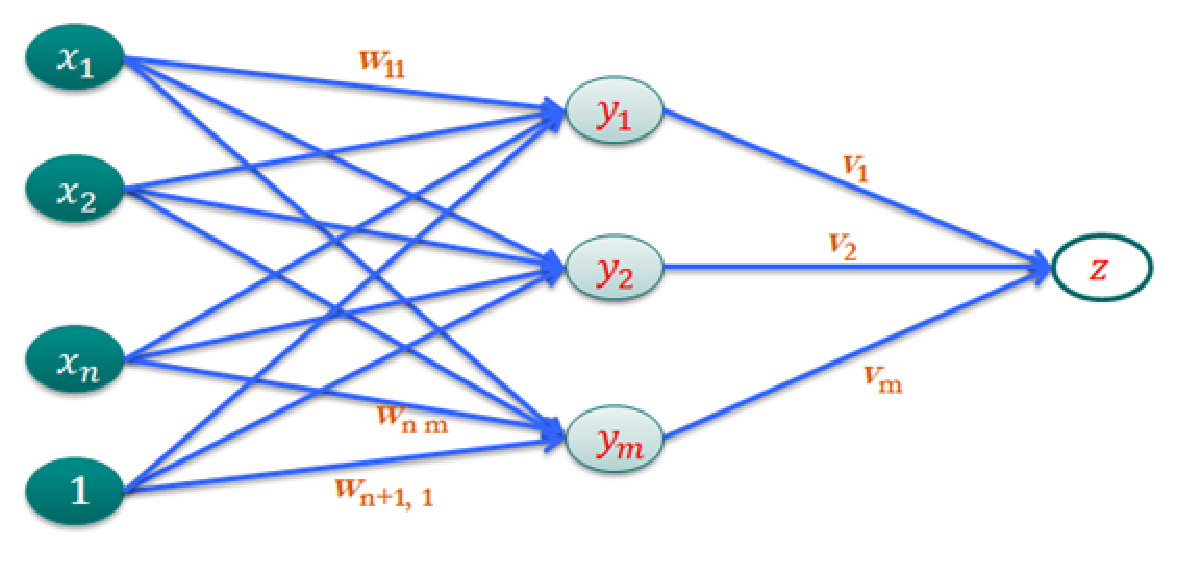
\includegraphics[width=0.65\textwidth,height=6cm]{figures/neuralnetwork.eps}
  \caption{三层神经网络}\label{fig:neuralnetwork}
\end{figure}

典型的神经网络,将神经元划分为三种类型:输入层(Input Layer)、隐藏层(Hidden Layer)、输出层(Output Layer)。每一层都包含多个神经元。输入层主要是用于数据的传递入口;输出层用于输出网络预测的结果;隐藏层是神经网络最吸引人的一层,是神经网络具有强大模拟和学习能力的一个主要因素。
图~\ref{fig:neuralnetwork}是一个典型的三层神经网络,包含$n$个输入神经元,$m$个隐藏神经元,1个输出神经元。箭头方向表示前向传播路径,每一条路径代表一个“突触”,“突触”的权值表示两相邻层神经元关系的重要程度。每个神经元都包含一个激活函数(Activation Function)表示对输入信号的反应,常用的激活函数都是Sigmoid 类型,如Logistic函数,Hyperbolic Tangent函数等。

\section{神经网络简史}
1943年,心理学家Warren McCulloch和数理逻辑学家Walter Pitts\cite{mcculloch1943logical}提出第一个用数理语言描述大脑信息处理过程的计算模型(阈值逻辑或Mcculloch—Pitts神经元),并产生人工神经网络研究的第一次分化:一个方向偏重于生物处理过程,另一个则偏重于神经网络在人工智能方面的应用。
1949年,心理学家Donald Hebb\cite{hebb1968the}提出突触联系可变假设,奠定了神经网络学习算法的研究基础。
1957年,Frank Rosenblatt\cite{rosenblatt1957perceptron} 提出了著名的感知器模型,它是第一个完整的人工神经网络,第一次把神经网络研究付诸工程实现,应用于模式识别、联想记忆等领域,一度有上百家实验室投入研究,美国军方甚至认为神经网络工程比“原子弹工程”更重要,给予巨额资助,并在声纳信号识别等领域取得一定的成绩。
1960年,Bernard Widrow和Marcian Hoff\cite{widrow1960adaptive} 提出自适应线性单元(ADAptive LINear Element, AdaLine),可用于自适应滤波、预测和模式识别,使得人工神经网络的研究进入第一个高潮。
1969年, Marvin Minsky和Seymour Papert\cite{minsky1969perceptron}指出单层感知器表示能力有限,无法处理线性不可分的问题,如异或判断,而多层感知器又过于复杂,按照当时计算机的处理能力根本无法实现。神经网络的研究受此影响,进入长达10年的萧条期。
1982年,Teuvo Kohonen\cite{kohonen1982self}总结大脑神经细胞的自组织特性、记忆方式以及神经细胞兴奋刺激的规律,提出著名的自组织映射(Self-Organizing Map, SOM)理论。
1982年,John Hopfield\cite{hopfield1982neural}用能量函数的思想提出一种新的计算方法,阐明了神经网络与动力学的关系,并用非线性动力学的方法来研究这种神经网络的特性,建立了神经网络稳定性判据,并指出信息存储在网络中神经元之间的连接上,形成了离散Hopfield网络。
1984年\cite{hopfield1984neurons},他又设计与研制了Hopfield网络模型的电路,指出神经元可以用运算放大器来实现,所有神经元的连接可用电子线路来模拟,并称之为连续Hopfield网络。他的研究成果有力推动了神经网络的发展,掀起神经网络研究的又一次热潮。
1984年,David Ackley和Geoffrey Hinton
\footnote{深度学习泰斗、多伦多大学特聘教授、爱丁堡大学人工智能博士,2012年获得加拿大国家最高科学奖,有“加拿大诺贝尔奖”之称的Killam 奖。}
等人\cite{ackley1985learning}将模拟退火算法引入神经网络,提出Boltzmann机网络模型,提供了一种有效的神经网络优化方法。
1986年,Rumelhart等人\cite{rumelhart1986learning}提出了误差反向传播算法(Back Propagation,BP),成为至今为止影响最大的一种网络学习方法。事实上早在1974 年,Paul Werbos\cite{werbos1974beyond}就在博士论文中首次给出了训练一般网络的反向传播学习算法,但一直不为人知。

BP网络存在两种基本的行为:前向传播和反向更新。前向传播表示神经元对信号的传播路径是单向的,从输入层逐层往下一层传播,直至从输出层获取输出信号的过程。反向更新是按照从输出层向隐藏层,从最后一个隐藏层向前一个隐藏层的顺序,从第一个隐藏层向输入层,逐层调整“突触”的权值过程。在监督学习中,反向更新实际上是对前向传播预测偏差的一种反馈和调整,以期达到逐步优化模型的目的。

利用BP算法网络可以从大量的训练样本学习统计规律,从而对未知事件做出预测,具有明显的优越性。90年代,各种机器学习模型相继诞生,如SVM、Boosting、最大熵方法(如逻辑回归)等,它们的结构基本上可以看成是含有单层隐藏节点(SVM、Boosting),甚至没有隐藏节点(逻辑回归)的模型,在小样本和有限计算单元时对复杂函数的表示能力有限,对于复杂问题泛化能力也受到一定制约,因此也被称为\textbf{浅层学习}(Shallow Learning)。

\section{深度学习}
2006年,机器学习领域的泰斗Geoffrey Hinton和他的学生Ruslan Salakhutdinov在《科学》上发表的一篇文章\cite{hinton2006reducing},掀起深度学习的研究浪潮。深度学习通过神经网络模拟人的大脑学习过程,从底层特征中逐层自动学习合并生成具有隐含语义的深层特征,根据大脑的多层抽象机制实现对数据(音频、图片和文本等)的抽象表达。深度学习已经在多个应用人工智能领域,如语音识别(Speech Recognition)、计算机视觉(Computer Vision)和自然语言处理(Nature Language Processing,NLP)取得重大进展,学术研究成果已经成功地应用到产业化流程,诞生了Siri、Android语音识别系统。

2012年,Google在透漏的技术路线图中明确表示要将下一阶段的技术重心放到\textbf{深度学习与知识图谱}(Knowledge Graph)。2012年6月,《纽约时报》披露了Google Brain项目,由斯坦福大学机器学习教授Andrew Ng和大规模计算机系统专家Jeff Dean共同主导,Google Brain使用16,000个CPU Core的并行计算平台模拟神经网络系统,在语音识别和图像识别等领域获得了巨大的成功。2012年12月,Hinton教授在多伦多大学的研究团队使用卷积神经网络深度学习系统,参加被誉为计算机视觉圣杯的ImageNet 大赛并大比分(16\% v.s. 26\%)领先。2013 年3 月,Google收购Hinton团队创立的DNNResearch
\footnote{DNNResearch是一家专注于语音和图像识别技术的研究公司。},
改善Google 图片搜索质量。2013年7月31日,Google发布用于自然语言处理的word2vec。2013年1月,百度成立深度学习研究院(Institute of Deep Learning,IDL),前Facebook资深科学家徐伟、人工智能领域专家余凯、美国新泽西州立大学统计系教授张潼、前AMD 异构计算专家吴韧陆续加盟百度IDL。2013年12月,Facebook成立人工智能实验室,并聘请Yann LeCun
\footnote{深度学习大拿,Hinton教授多伦多大学的博士后,纽约大学终身教授,纽约大学数据科学中心负责人。他在巴黎第六大学(也称皮埃尔玛丽居里大学)Paris VI (Universit\'{e} Pierre et Marie Curie)获得计算机科学博士学位,期间提出反向传播算法。在加盟Facebook之前,他已经在贝尔实验室工作20多年,期间使用卷积神经网络CNN开发出一套手写数字识别系统LeNet,拥有14项发明专利。}
教授坐镇指导。与LeCun一起加入的还有纽约大学计算机科学系副教授Rob Fergus,他的学生Matthew Zeiler 创立一家专门提供图像搜索服务的公司Clarifai,其研发的深度学习算法在2013年ImageNet大赛保持领先。2013 年12月13日,Mark Zuckerburg 与俄罗斯富豪Yuri Milner 出资300万美元设立Breakthrough Prize in Mathematics奖项。

传统的神经网络采用反向传播方式进行,利用迭代算法训练整个网络:随机设定初值,计算当前网络的输出,根据它与真实标签间的差异反向更新网络各层参数,直至收敛。深度学习为克服神经网络训练速度慢、容易过拟合的问题,采用迥然不同的逐层(Layer-wise)训练机制,从而避免深层反向传播误差校正信号减弱,出现梯度扩散
(Gradient Diffusion)现象。

一般地,信号处理(以图像处理为例)都包括以下几个流程(见图\ref{fig:featurelearning}):
\begin{itemize}
    \item 预处理:对输入图像放缩、去噪、背景差分等。
    \item 特征处理:在预处理后的数据上进行特征提取、特征选择、特征降维等工作。
    \item 模型训练:根据图像的特征向量,学习和训练模型。
\end{itemize}
通常,前两步统称为“特征学习”。
\begin{figure}[htbp]
  \centering
  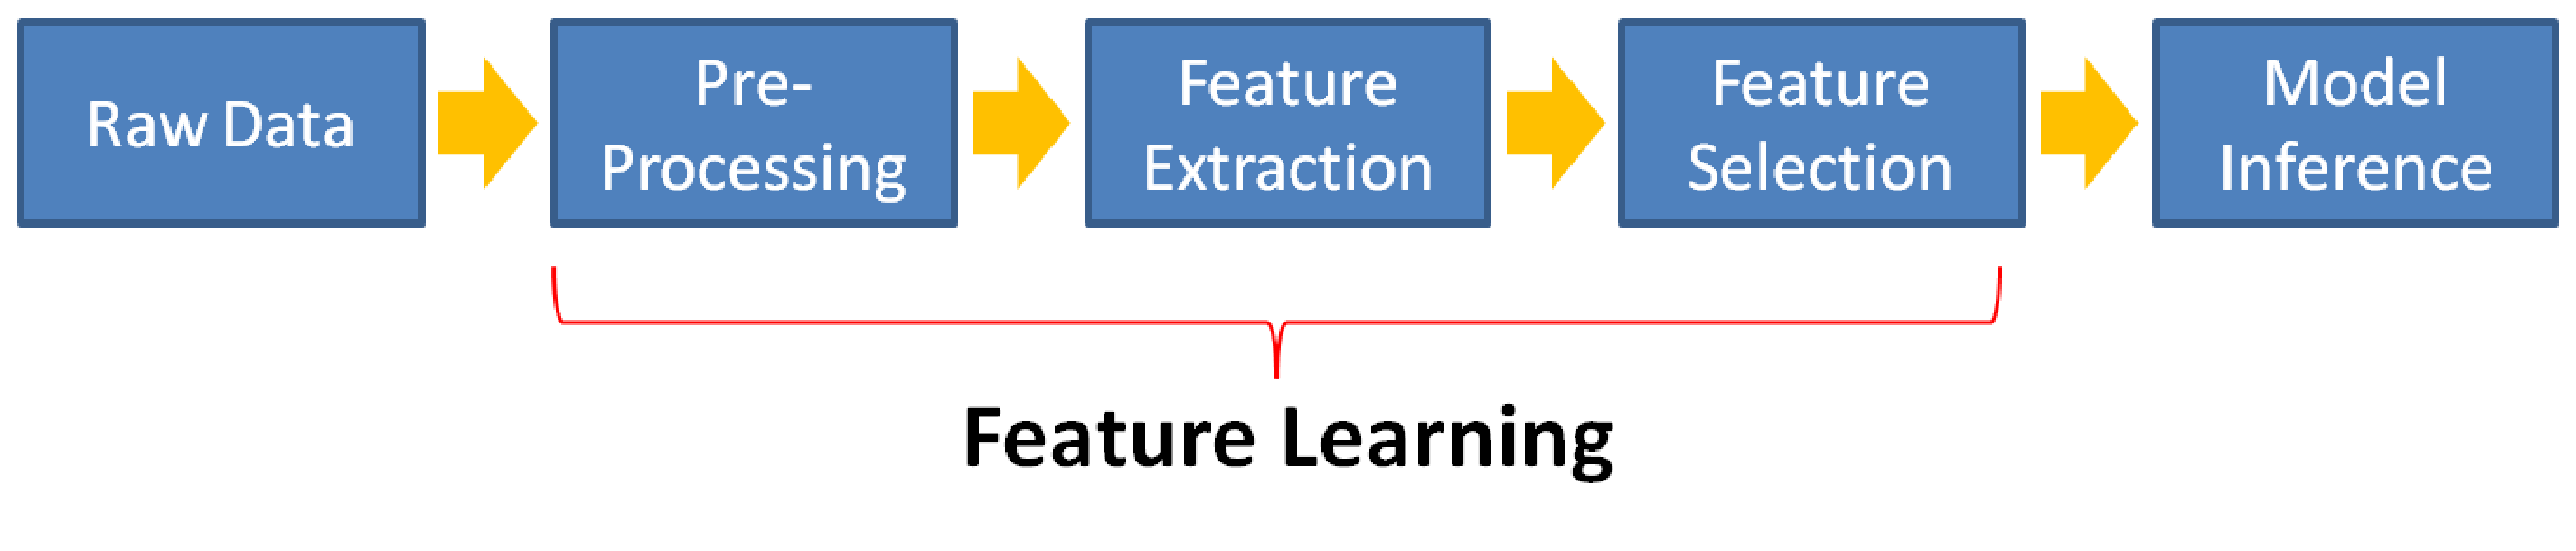
\includegraphics[width=0.85\textwidth,height=2cm]{figures/featurelearning.eps}
  \caption{信号处理流程}\label{fig:featurelearning}
\end{figure}
在流程图中我们看出,后续操作均建立在前面输出结果的基础之上,越是靠前的处理愈加重要,不考虑预处理,特征提取是其中最为重要的部分。特征提取需要大量的人工参与,既增加了特征的不确定性,也产生了大量人力开销。研究人员期望直接从原始数据中学习特征,于是发展出深度学习的概念,距离人工智能的目标又近了一步。深度学习的“无监督特征学习”、“特征学习”之别称由此得名。

假设一个系统$S$有$n$层$S_1,S_2,\ldots,S_n$,系统输入是$I$,输出为$O$,形象地我们可以将其表示成:
\begin{equation}
    I \Rightarrow S_1 \Rightarrow S_2\Rightarrow \cdots \Rightarrow S_n \Rightarrow O
\end{equation}
如果$O=I$,即输入$I$经过系统变化后无任何信息损失,则意味着经过每一层$S_i$,输入$I$都没有任何信息损失,$S_i$可看做原有输入信息$I$的另一种表示。假设有一组输入,并设计了系统$S$,通过调整系统中的参数,使得系统输出$O=I$,由此可自动地获取输入$I$的一系列层次的特征表示$S_1,S_2,\ldots,S_n$。

深度学习常用的方法有Auto Encoder、Sparse Coding和受限Boltzmann机,我们将在后文陆续介绍。

\subsection{自动编码器}
人工神经网络自身就是具有层次结构的系统,给定一个神经网络,假设其输出与输入是相同的,通过训练、调整参数,可以确定每层的权重,代表输入$I$的一层表示。将输入$I$ 的多层表示作为新的特征添加到原始特征中,实验表明有利于改善模型的预测精度,在分类问题中甚至比目前最好的分类算法效果还要好。我们所描述的这种方法称为自动编码器(Auto Encoder)。如果在自动编码器的基础上添加约束性条件,如$\ell_1-$规则化约束,就是“稀疏的自动编码器”方法。

\subsection{稀疏编码方法}
“输出$O$严格地等于输入$I$”的限制略微放松,比如只要二者的差别尽可能地小,由此衍生出一类方法,即稀疏编码(Sparse Coding)方法。假设$b_1,\ldots,b_n$ 是基,输出$O$使用基线性表示:
\[
    O = \sum\limits_{i=1}^n \omega_i b_i
\]
其中,$\omega_i$是基$b_i$的系数,则我们可以得到下面形式的优化问题:
\begin{equation}\label{eq:sparsecode}
    \begin{array}{ll}
      \min\limits_{\omega,b} & \|I-O\|
    \end{array}
\end{equation}
通过解决最小化问题,得到最优的系数与基,它们就是输入$I$的一种近似表达,可以作为特征表示输入。如果对问题\eqref{eq:sparsecode}添加$\ell_1-$规则项:
\begin{equation}\label{eq:regsparsecode}
    \begin{array}{ll}
      \min\limits_{\omega,b} & \|I-O\| + \lambda\sum\limits_{i=1}^n |\omega_i|
    \end{array}
\end{equation}
将一个信号表示为一组基的线性组合,只需要较少的几个基即可近似表示原始信号。

\subsection{玻尔兹曼机}
神经网络是由大量神经元组成的动力学系统。从宏观上看,各神经元的状态可看作是一个随机变量,正如统计物理学中,把大量气体分子看作一个系统,每个分子状态服从统计规律。从统计观点分析,也可寻找神经网络系统中某种神经元的状态的概率分布,分布的形式与网络的结构有关,其参数则是权系数。Hinton等人~\cite{hinton1983optimal}借助统计物理学的方法提出了玻尔兹曼模型,可用于模式分类、预测、组合优化及规划等方面。

1986年,Hinton和Sejnowski~\cite{hinton1986learning}发展出受限玻尔兹曼机(Restricted Boltzmann Machine, RBM),成为机器学习的一个重要工具。RBM属于
\textbf{生成型随机神经网络模型},同普通神经网络类似,包括三层结构:输入层、输出层与隐藏层,由于输入层与输出层可见,称作可见单元(Visible Units),对应地称隐藏层为隐藏单元(Hidden Units)。在图\ref{fig:rbm}中,玻尔兹曼机含有12个可见单元(构成向量$v$)和3个隐藏单元(构成向量$h$)。RBM网络的每一对神经元之间的进行双向对称的信息传递,权值矩阵$W=(w_{ij})$对称,并且自身无反馈$w_{ii}=0$。在RBM网络图上,可见变量与隐藏变量均是二元变量,状态取值范围是$\{0,1\}$。
\begin{figure}[htbp]
  \centering
  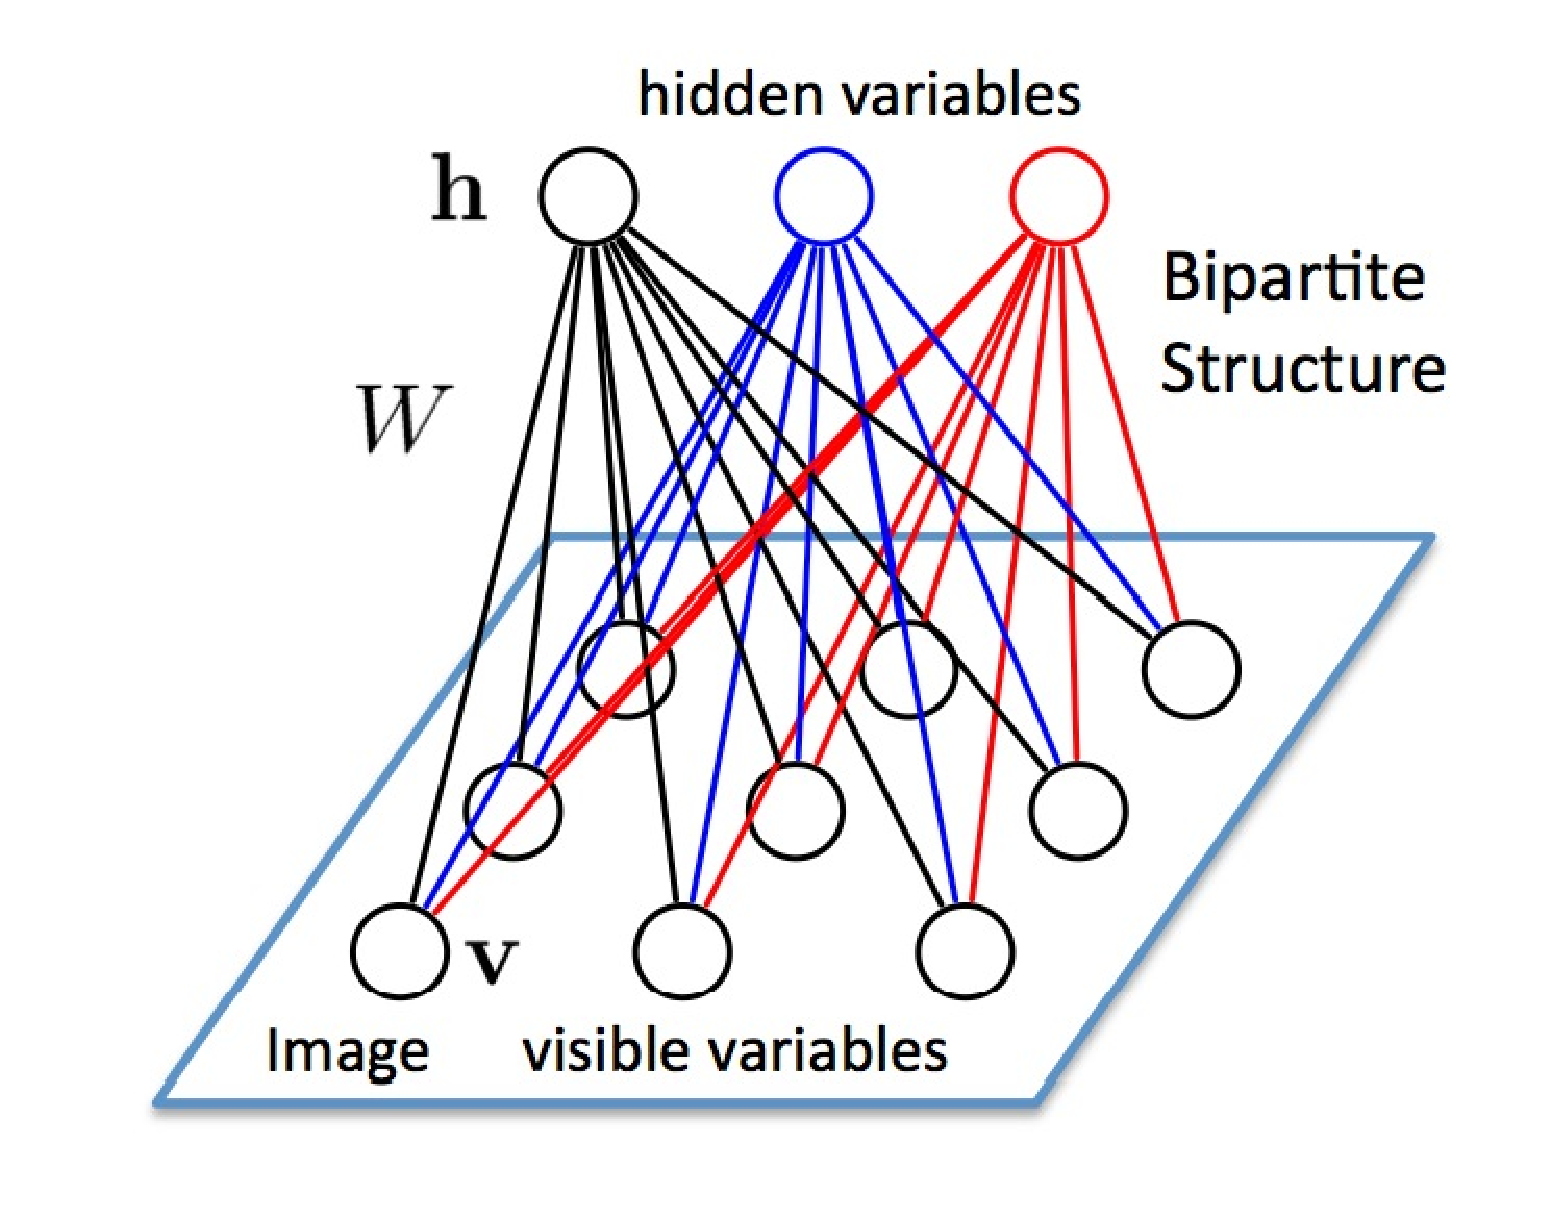
\includegraphics[width=0.5\textwidth, height=5cm]{figures/rbm.eps}
  \caption{受限Boltzmann机}\label{fig:rbm}
\end{figure}

RBM对网络配置$(v,h;\theta)$定义了能量的概念,数学表示如下:
\begin{equation}\label{eq:rbm-energy}
    E(v,h;\theta) = - \sum\limits_{i}\sum\limits_{j} w_{ij} v_i h_j - \sum\limits_{i} a_i v_i - \sum\limits_{j} b_j h_j
\end{equation}
其中,$a_i,b_j$分别表示可见单元$v_i$,隐藏单元$h_j$的偏置权重,$\theta$表示网络参数集。

根据配置能量的定义,RBM给出下面形式的网络配置概率分布
\begin{equation}
    P_{\theta}(v,h) = \frac{1}{Z(\theta)} \exp\big(-E(v,h;\theta)\big)
\end{equation}
其中,$Z(\theta)$表示归一化因子,也称\textbf{配分函数}(Partition Function)。将式子~\eqref{eq:rbm-energy}代入概率分布,可得:
\begin{equation}\label{eq:rbm-distribution}
    P_{\theta}(v,h) = \frac{1}{Z(\theta)} \exp\big(\sum\limits_{i}\sum\limits_{j} w_{ij} v_i h_j + \sum\limits_{i} a_i v_i + \sum\limits_{j} b_j h_j\big)
\end{equation}
对隐藏层上所有可能的配置加和,可计算观测数据的似然函数
\begin{equation}
    P_{\theta}(v) = \frac{1}{Z'(\theta)} \sum\limits_{h} \exp\big(v^T W h + a^T v + b^T h\big)
\end{equation}
并构造对数似然估计函数
\begin{equation}\label{eq:likelihood-estimation}
    L(\theta) = \frac{1}{|V|} \log(\prod\limits_{v\in V} P_{\theta}(v)) = \frac{1}{|V|} \sum\limits_{v\in V} \log(P_{\theta}(v)).
\end{equation}
其中,
\[
    Z'(\theta) = \sum\limits_{v} \sum\limits_{h} \exp\big(v^T W h + a^T v + b^T h\big)
\]
表示归一化项。根据最大似然估计方法,计算对数似然函数的梯度
\begin{equation}
    \begin{array}{lll}
      \partial L(\theta)/\partial w_{ij} & = & \frac{1}{|V|}  \sum\limits_{v\in V} \partial \log(P_{\theta}(v))/\partial w_{ij} = \frac{1}{|V|} \sum\limits_{v\in V} \frac{1}{P_{\theta}(v)} \frac{\partial P_{\theta}(v)}{\partial w_{ij}} \\
       & = & \frac{1}{|V|} \sum\limits_{v\in V} \frac{1}{P_{\theta}(v) Z'(\theta)} \big\{\sum\limits_{h} \exp\big(v^T W h + a^T v + b^T h\big) v_i h_j - P_{\theta}(v) \frac{\partial Z'(\theta)}{\partial w_{ij}} \big\}
   \end{array}
\end{equation}
由于
\begin{equation}
    \partial Z'(\theta)/\partial w_{ij} = \sum\limits_{v} \sum\limits_{h} \exp\big(v^T W h + a^T v + b^T h\big) v_i h_j
\end{equation}
若记
\begin{equation}
    P'_{\theta} = \frac{\exp\big(v^T W h + a^T v + b^T h\big)}{\sum\limits_{h} \exp\big(v^T W h + a^T v + b^T h\big)} = \frac{\exp\big(v^T W h + a^T v + b^T h\big)}{P_{\theta}(v) Z'(\theta)}
\end{equation}
则有
\begin{equation}
    \begin{array}{lll}
      \frac{\partial L(\theta)}{\partial W_{ij}} & = & \frac{1}{|V|} \sum\limits_{v\in V} \bigg[P'_{\theta} v_i h_j - P_{\theta}v^T h\bigg] \\
      & = & \mathbb{E}_{P'_{\theta}} (v_i h_j) - \mathbb{E}_{P_{\theta}} (v_i h_j)
   \end{array}
\end{equation}
成立。由于计算开销较大,Hinton~\cite{hinton2002training}提出了一种高效的学习算法:\textbf{对比散列}(Contrastive Divergence, CD)。

如果增加受限玻尔兹曼机隐藏层的层数,就是\textbf{深度玻尔兹曼}(DBM)。如果在靠近可视层处使用\textbf{贝叶斯信念网络}(Bayisian Belief Network,BBN,表示有向图模型),在离可视层最远处使用受限玻尔兹曼机,就是\textbf{深度信念网络}(Deep Belief Network,DBN)。

\section{信念网络}
1985年,Judea Pearl提出贝叶斯网络,也称信念网络(Belief Network)。它是一种模拟人类推理过程中因果关系的不确定性处理模型,其网络拓朴结构是一个有向无环图(Directed Acyclic Graphic, DAG)。它的节点用随机变量或命题来标识,认为有直接关系的命题或变量则用弧来连接。

\section{卷积神经网络}
卷积神经网络(Convolutional Neural Networks, CNN)是一种特殊的深层神经网络模型,网络中神经元并非完全连接,同一层部分神经元之间共享连接权重。卷积神经网络稀疏连接(Sparse Connectivity)和权值共享(Shared Weights)的结构特性更接近生物神经网络,有效降低了网络模型的复杂度。

CNN源于视觉神经机制,为识别二维图形而设计出的一种多层感知器,对平移、比例缩放、倾斜或其他形式的变形具有高度不变性。1962 年,David Hubel和Torsten Wiesel 研究猫视觉皮层细胞时,提出了感受野(Receptive Field)概念;1984年,日本学者Kunihiko Fukushima基于感受野提出神经认知机(Neocognitron)模型。神经认知机将一个视觉模式分解成多个子模式(特征),进入分层递阶式相连的特征平面进行处理,在物体发生位移或轻微变形时,也能进行识别。神经认知机模型是第一个CNN模型,后来成功应用到手写数字识别、车牌识别和人脸识别等领域。

\chapter{极限学习机}
2006年,Huang Guang-Bin等人\cite{huang2006extreme}在单隐层前向神经网络(Single Hidden Layer Feed-forward Neural Networks,SLFNs)基础上提出一种高效的学习方法,称作\textbf{极限学习机}(Extreme Learning Machine,ELM)。

在传统的神经网络模型中,所有网络中的参数都需要调整,不同层之间存在相互依赖关系。对于前向神经网络模型中,主要使用梯度下降法调整模型参数。梯度下降法存在一个比较常见的问题,迭代步长设置的太小则收敛速度放慢,设置的太大则容易陷入局部最优点。ELM算法不需要调整所有的参数,它随机产生隐藏层权值(输入与隐藏层),并通过解矩阵的广义逆确定输出权值(隐藏层与输出层)。

给定任意$N$个训练样本$(x_i,y_i)$,$i=1,2,\ldots,N$,$x_i\in \mathbb R^n$为输入向量,$y_i\in \mathbb R^m$表示输出向量。对于标准的存在$L$个隐藏节点的前向神经网络模型可以表示成下面形式的数学模型:
\begin{equation}
    f(x) = \sum\limits_{i=1}^L \beta_i g_i(x) = \sum\limits_{i=1}^l \beta_i g(\omega_i^T x + b_i)\in \mathbb R^m
\end{equation}
对于第$i$个隐藏节点,它与输入节点的链接权值向量为$\omega_i\in \mathbb R^n$,它的偏置量(阈值)为$b_i$,它与输出节点链接权值向量为$\beta_i \in \mathbb R^n$,隐藏层的激活函数为$g$,输出层的激活函数是线性函数。给定输入$x\in \mathbb R^n$,模型的第$j$维输出为
\begin{equation}
    f_j(x) = \sum\limits_{i=1}^L \beta_{ij} g_i(x),\quad j = 1,2,\ldots,m.
\end{equation}
对于$N$个输入样本,我们使用向量形式表示单层前向神经网络模型:
\begin{equation}
    f(X) = H \beta
\end{equation}
其中,$H$称作神经网络的隐藏层输出矩阵,具体地
\begin{equation}
    H =
    \begin{bmatrix}
    g(\omega_1^T x_1 + b_1) & g(\omega_2^T x_1 + b_2) & \ldots & g(\omega_L^T x_1 + b_L)\\
    g(\omega_1^T x_2 + b_1) & g(\omega_2^T x_2 + b_2) & \ldots & g(\omega_L^T x_2 + b_L)\\
    \vdots & \vdots & \ddots & \vdots\\
    g(\omega_1^T x_N + b_1) & g(\omega_2^T x_N + b_2) & \ldots & g(\omega_L^T x_N + b_L)\\
    \end{bmatrix}
\end{equation}
如果隐藏层激活函数在任何区间都是无限次可微(Infinitely Differentiable),那么对于任意$N$个不同的输入样本$(x_i,y_i)$,对于任意随机生成的$\omega_i$ 与$b_i$,隐藏层输出矩阵$H$都是可逆矩阵\cite{huang2006extreme}。SLFN模型可以零误差逼近$N$个输入样本,即满足
\begin{equation}
    H\beta = Y.
\end{equation}
传统神经网络模型大多都是基于梯度下降法调整模型参数,SLFN模型随机选择参数$\omega$与$b$,并通过求解最小范数最小二乘问题
\begin{equation}
    \min\limits_{\beta}~\|H\beta - Y\|
\end{equation}
确定Moore-Penrose广义逆表示的最优解
\begin{equation}
    \hat \beta = H^{\dag} Y.
\end{equation}

为了处理分类问题,ELM建立下面形式的优化模型
\begin{equation}
    \begin{array}{ll}
    \min\limits_{\beta,\xi} & \frac{1}{2} \beta^T \beta + \frac{1}{2} C \sum\limits_{i=1}^N \xi_i^T \xi_i\\
    \textit{s.t.} & h(x_i) \beta = y_i^T - \xi_i^T,i = 1,2,\ldots,N
    \end{array}
\end{equation}
建立拉格朗日函数
\begin{equation}
    L(\beta, \xi, \lambda) = \frac{1}{2} \beta^T \beta + \frac{1}{2} C \sum\limits_{i=1}^N \xi_i^T \xi_i - \sum\limits_{i=1}^N \lambda_i (h(x_i) \beta - y_i^T + \xi_i^T)
\end{equation}
根据KKT条件可以得到优化模型的解析解:
\begin{equation}
    \beta = H^T (C^{-1} I + HH^T)^{-1} Y,
\end{equation}
以及输出模型
\begin{equation}
    f(x) = h(x) H^T (C^{-1} I + HH^T)^{-1} Y,
\end{equation}
将其应用于多元分类,我们可以得到决策模型
\begin{equation}
    \hat y_x = \argmax\limits_{i\in\{1,\ldots,m\}} f_i(x).
\end{equation}

\chapter{决策树}
决策树是一种重要的数据表示、决策分析和预测技术,常用于辅助分析决策,学习构造决策模型,在运筹学、数据挖掘、机器学习领域中应用广泛。决策树的优点包括直观易懂、预测准确率高、稳定性好,决策树的成长不需要任何领域知识或参数设置,适用于探索式的知识发现应用。

每一颗决策树都有根节点、内部节点、叶子节点,及连接节点的树枝。如果使用决策树表示一个预测模型,那么根节点表示全部数据集合,每个内部节点表示样本的一个属性,每根树枝则代表对属性的一种判断(测试)结果,每个叶子节点对应一个决策目标(类别标签)。沿着树根到达任意一个叶子节点所经过的路径,就是一个决策(预测)规则。我们在这一节主要介绍和讨论用于数据挖掘的决策树方法。

最早的决策树算法是由Hunt等人\cite{hunt1966experiments}于1966 年提出的概念学习系统(Concept Learning System,CLS)。目前最具影响的是John Quinlan提出的ID3 算法\cite{quinlan1986induction}与C4.5算法\cite{quinlan1993c4}。ID3 算法的目的在于减少树的深度,但忽略了叶子数目的研究。C4.5算法在ID3 算法的基础上进行了改进,对于预测变量的缺值处理、剪枝技术等方面作了较大改进,既适合于分类问题,又适合于回归问题。根据决策树预测结果的数据类型,可以将决策树分成:分类树和回归树,前者预测的是离散型数据,而后者预测的是连续型数据,并且两类决策树的生成方式也不同。ID3与C4.5是两个典型的决策树分类算法,在数据挖掘与机器学习领域还存在其他一些著名的决策树算法,如1980年Gordon Kass\cite{kass1980exploratory}在其博士论文中提出的卡方自动交互检测算法(CHi-squared Automatic Interaction Detection,\textbf{CHAID}),1984年Leo Breiman等人\cite{breiman1993classification}提出的分类回归树(Classification And Regression Tree,\textbf{CART}),1991年Jerome Friedman\cite{friedman1991multivariate}发展的多元自适应回归样条模型(Multivariate Adaptive Regression Splines,\textbf{MARS})。

决策树的生长是一个自顶向下,分而治之的递归过程,在数据集$S$ 上,树的生长基本流程如下:
\begin{itemize}
  \item 如果$S$中所有样本都属于同一类或满足其他停止生长准则,则$S$不再划分,生成叶子节点。
  \item 否则,根据一个指标选择合适的属性与分裂节点,对$S$进行划分,产生多个样本子集$S_i,i=1,2,\dots$,并对每个样本子集$S_i$执行以上两步。
\end{itemize}
在决策树的生长过程,每步选择一个变量对样本做\textbf{最佳划分},衡量划分质量的性能指标,包括ID3算法使用的信息增益、C4.5 使用的信息增益率、CART 算法使用的Gini混杂度(Gini Impurity, GI)和CHAID算法使用的$\chi$值。

\begin{example}
Gore Forest是一家高尔夫俱乐部的经理,他希望通过天气预测人们是否打高尔夫球,以适时调整雇员数量减少开支。为此,他记录了两周内天气情况与高尔夫运动的统计数据(见表~\ref{tbl:golf})。记录的数据中,天气状况包括Outlook(sunny,overcast,rain),Temperature(64--85),Humidity(65--96),Windy
(yes,no)四个变量;类标变量是二元的,表示人们是否打高尔夫。根据统计数据,我们可以构建如图~\ref{fig:decisiontree}所示二元分类决策树模型。
\begin{table}[htbp]
    \centering
    \begin{tabular}{|l|c|c|c|c|c|}
      \hline
        Outlook & Temperature & Humidity & Windy & Play\\
        \hline
        sunny & 85 & 85 & no & no\\
        \hline
        sunny & 80 & 90 & yes & no\\
        \hline
        overcast & 83 & 78 & no & yes\\
        \hline
        rain & 70 & 96 & no & yes\\
        \hline
        rain & 68 & 80 & no & yes\\
        \hline
        rain & 65 & 70 & yes & no\\
        \hline
        overcast & 64 & 65 & yes & yes\\
        \hline
        sunny & 72 & 95 & no & no\\
        \hline
        sunny & 69 & 70 & no & yes\\
        \hline
        rain & 75 & 80 & no & yes\\
        \hline
        sunny & 75 & 70 & yes & yes\\
        \hline
        overcast & 72 & 90 & yes & yes\\
        \hline
        overcast & 81 & 75 & no & yes\\
        \hline
        rain & 71 & 80 & yes & no\\
      \hline
    \end{tabular}
    \caption{天气状况与高尔夫运动状况关联表}
    \label{tbl:golf}
\end{table}

\begin{figure}[htbp]
  \centering
  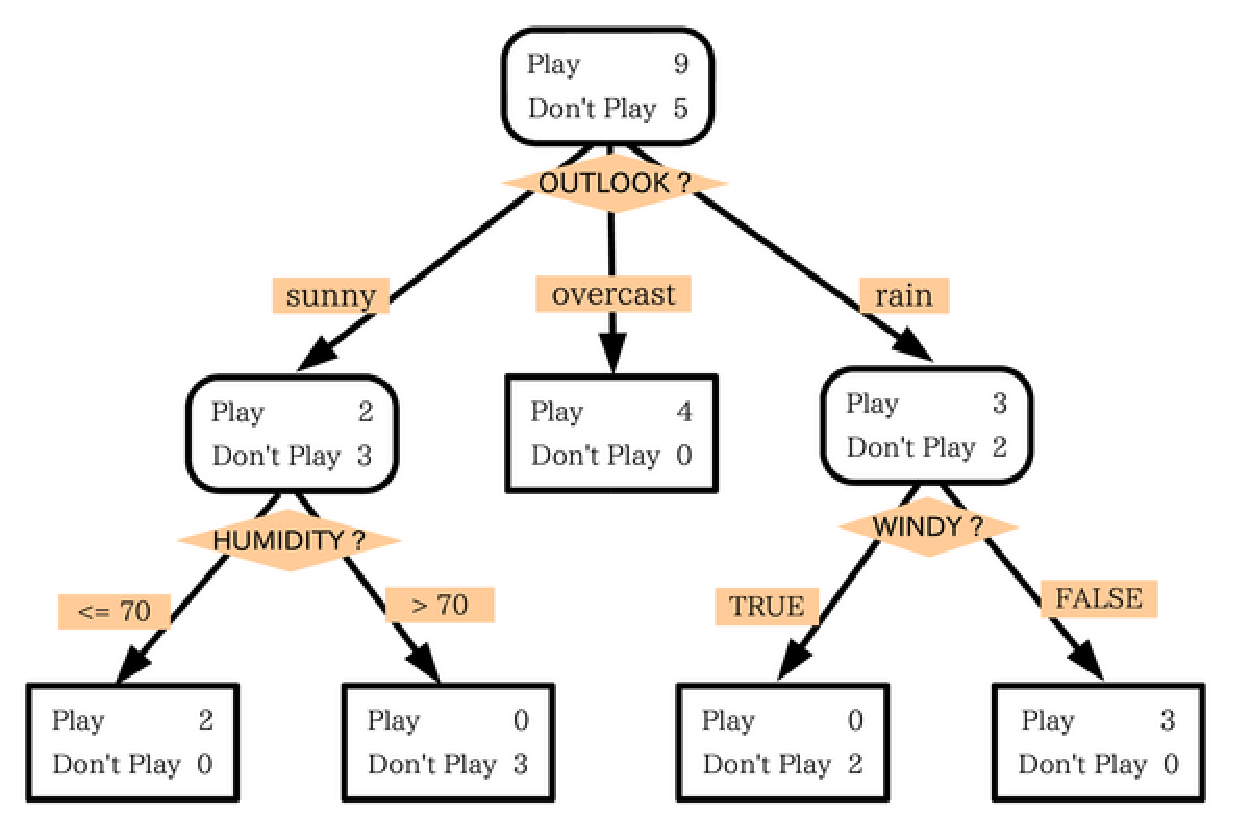
\includegraphics[width=0.85\textwidth]{figures/decisiontree.eps}
  \caption{决策树预测模型}\label{fig:decisiontree}
\end{figure}

\end{example}

\subsection{决策树桩}
决策树桩(Decision Stump)是最简单的二叉树,只含有两个叶子节点,在单个特征上做出决策,是一种简单有效的机器学习算法,如集成算法中常用作基本模型,独立使用时,可用于筛选变量、搜寻连续变量上具有预测意义的节点等。

\subsection{剪枝}
在实际应用中,采集的数据可能存在噪声和异常点(离群点或孤立点),可能导致决策树模型过拟合。为此,可以对决策树剪枝(Pruning),剪掉不重要的节点以简化决策树模型,提高决策树的泛化能力。常见的剪枝策略是\textbf{预剪枝}(Pre-Pruning, Early Stop Rule)和后剪枝(Post-Pruning),前者是在决策树生长的同时根据一定指标确定停止生长的节点,后者则是在决策树长成后,遍历决策树剪掉符合剪枝条件的节点。对于剪枝后的分类决策树,叶子节点的类别根据多数投票准则确定。

\textbf{预剪枝}:在预剪枝方法中,最直接的方法设置决策树生长的最大深度,使决策树无法充分生长。但是,如何选择合适的深度是一个及其重要的问题。此外,还有一个方法是检验当前结点对应的样本集合,如果集合中样本数量小于预先指定的阈值,则将当前结点设为叶子结点并停止生长。

\textbf{后剪枝}:后剪枝技术是指在完全长成的决策树上,根据一定的指标剪掉树中冗余的子树,形成一棵约简的新树,与树的生长顺序相反自底向上地剪枝。决策树算法ID3、C4.5和CART 主要采用后剪枝技术。后剪枝策略使用一组测试数据用于检验剪枝操作的合理性,一边修剪一边检验,其基本原则是\textbf{确保每次剪枝后,决策树在测试集上的预测精度至少不会下降}。

\subsection{缺值}
实际采集的数据中可能出现缺值,处理缺值问题比较常见的方法是给它赋值,如数据集中相应属性均值、最大值、最小值等,C4.5算法则将一个概率分布向量赋予它。比如,对于二元属性$A$,数据集中12个样本属性值$A=0$,88个样本属性值$A=1$,C4.5根据数据集中样本在属性值$A$上的分布,推断属性$A$缺失的值为0的可能性是12\%,为1 的可能性是88\%。利用缺值的概率分布,有助于选择合适的分裂节点。

\subsection{树的集成模型}
目前,集成技术在机器学习领域颇受青睐,如Bagging决策树、随机森林、提升树和旋转森林(Rotation Forest)都是通过构造多个决策树做模型聚合。

\section{ID3和C4.5}
1986年,Ross Quinlan提出ID3(Iterative Dichotomiser 3)算法\cite{quinlan1986induction},它是目前最具影响力的决策树算法。1993年,Quinlan对ID3进行改进,发展为C4.5算法\cite{quinlan1993c4},能够同时处理离散型与连续型属性。ID3与C4.5均属于归纳(Inductive)模型,假设训练数据与测试数据服从相同的未知分布。

ID3算法源于概念学习系统思想,对于训练集$S$,概念学习系统基本步骤包括:
\begin{enumerate}[Step 1.]
  \item 如果$S$中的所有样本都是正例(或负例),则创建yes(no)叶子节点,停止算法;
  \item 如果$S$中正负例都有,则由专家选择一个分裂属性$A=\{a_1,\ldots,a_m\}$,创建中间节点;
  \item 根据属性$A$将输入样本空间分割成$m$个子集:$S_1,\ldots,S_m$;
  \item 对每个子集,重复以上步骤。
\end{enumerate}
概念学习系统在创建中间节点是由专家选择分割属性,带有明显的主观性。为此,ID3算法根据信息增益自动搜索分割节点(属性)。

对于分类问题,假设训练集是$S=\{x_i,y_i\}_{i=1}^N$,其中$x_i$ 是一个多属性向量,属性可以是离散的也可以是连续型,$y_i=\{1,\ldots,K\}$是分类变量。对于训练集$S$,根据统计的样本类别分布$\{p_k\}_{k=1}^K$,可以计算数据分类所包含的信息熵:
\begin{equation}
    H(S) = -\sum\limits_k p_k \log p_k
\end{equation}
其中,$p_k$表示类别$y=k$的样本比例,$\sum\limits_k p_k = 1$。 在信息论中,熵也是衡量混杂程度的指标,当类别分布为均匀分布时,分类状态最混杂,数据包含的信息熵最大。比如,对于前述高尔夫球运动预测的例子,打高尔夫的比例$p_1=9/14$,不打高尔夫的有$p_2=5/14$,则分类属性包含的信息熵:
\begin{equation}
    H(S) = -9/14 \log(9/14) - 5/14 \log(5/14) = 0.94
\end{equation}

决策树生长过程,最核心的一步是选择合适的属性(值)作为分裂点。ID3算法根据“Occam剃刀理论”,选择信息增益最大的属性作为分裂点,构建一棵深度最浅、完全分裂的决策树。根据属性$A=\{a_1,\ldots,a_m\}$,可以将输入的样本空间分割成$m$个子空间:$S_1,\ldots,S_m$,在每个子空间上都可以计算分类属性的信息熵,并根据各个子空间中样本比例计算属性$A$包含的平均信息熵。属性$A$产生的信息增益表示属性A包含的平均信息熵相对于整个输入空间上分类属性的信息熵的减少量(混杂度下降),具体地
\begin{equation}
    \textrm{IG}(S,A) = H(S) - \sum\limits_i \frac{|S_i|}{|S|} H(S_i)
\end{equation}
对于属性Outlook,其平均信息熵:
\begin{eqnarray}
  \text{H(S,Outlook)} &=& \frac{5}{14} \text{H(sunny)} + \frac{4}{14} \text{H(overcast)} + \frac{5}{14} \text{H(rain)}\\
  &=& 0.694.
\end{eqnarray}
同理,我们可以计算Windy的平均熵H(S,Windy)=0.892,属性Outlook 与Windy的信息增益分别是IG(S,Outlook) = 0.246,IG(S,Windy)=0.048。

ID3算法存在两个明显的缺陷:信息增益的计算要求数据属性是离散的,对于连续的数值属性,无法直接计算信息增益。ID3算法还倾向于多值属性,可能会产生无意义的分割。

对于离散型属性,C4.5算法与ID3的处理方法相同。对于连续型数值属性,C4.5算法对属性值进行离散化处理:假设数据集大小为$n$,根据数据集属性A列对数据样本进行升序排列,获得一个属性值序列$a_1<a_2<\ldots<a_m$。根据属性值序列确定$m-1$个分割点$s_1,\ldots, s_{m-1}$,第$i$个分割点取为$a_i$和$a_{i+1}$的均值,即
\[
    s_i = \frac{1}{2}(a_i + a_{i+1})
\]
每个分割点将属性序列值分割成两个子集:$[a_1,s_i)$与$(s_i,a_m]$,根据两个子集可以计算每个分割点产生的信息增益率(Information Gain Ratio),并选择信息增益率最大的分割点做树的分裂。信息增益率定义如下:
\begin{equation}
    \text{GR(S,A)} = \frac{\text{IG(S,A)}}{\text{SI(S,A)}}
\end{equation}
其中,SI(S,A)是属性A的分裂信息量(Split Information),反映数据关于属性A分布的均匀程度
\begin{equation}
    \text{SI(S,A)} = -\sum\limits_{i=1}^m \frac{|S_i|}{|S|} log \frac{|S_i|}{|S|}
\end{equation}
对于分布均匀的属性,分裂信息量比存在峰值的分布大。最极端的情况,每个样本在的A属性值均不同,则其信息增益最大。分裂信息量作为标准化项可以抵消掉分裂时对均匀分布属性的偏好。

在C4.5算法中,决策树的生长需要对数据集进行多次扫描和属性值排序,效率低下,而且训练数据需要读入内存,并不适合处理大数据集。C5.0算法进一步改进C4.5 算法在速度和空间利用方面均达到了工业化应用的标准。

\section{分类与回归树}
分类与回归树(Classification And Regression Trees, CART)是一种非参数决策树分类技术\cite{breiman1993classification}。CART 可以轻松处理离散和连续的属性,它的一个重要特点是对异常点不敏感,并且自变量的单调变换(如指数、对数变换)不影响决策树的生成、模型的构建。

CART的目标是生成一个完全树,树的叶子节点是同质的,归属于同一类别。在树的构建过程,树的分裂对于分类树与回归树是不同的。分类树的生成依据混杂度下降幅度最大选择分裂属性,如Gini指数、信息增益(率)。对于包含$K$个类别的样本数据集,Gini指数可以度量样本数据集关于类别进行分裂的混杂度
\begin{equation}
    \text{GI}(S) = 1- \sum\limits_{k=1}^K p_k^2
\end{equation}
对于给定属性A,将数据集分裂成$m$个子集$\{S_1,\ldots,S_m\}$,则基于它进行分裂的混杂度对应一个平均Gini指数
\begin{equation}
    \text{GI}(S,A) = \sum\limits_{i=1}^m \frac{|S_i|}{|S|} \text{GI}(S_i)
\end{equation}
分类树选择能够产生最大程度Gini指数降幅的节点作为分裂节点
\begin{equation}
    \Delta \text{GI}(S,A) = \text{GI}(S) - \text{GI}(S,A)
\end{equation}
回归树选择分裂节点的依据是最小化左右子树的平均方差
\begin{equation}
    \argmin\limits_{a}~[p_l \sigma^2_{y_l} + p_r \sigma^2_{y_r}]
\end{equation}
其中,$a$是属性A的一个属性值。一般地,如果选择它作为分裂节点,则将属性值A小于$a$的样本分到左子树,其他的分配到右子树。$p_l,p_r$分别表示左、右子树包含的样本比例,$\sigma^2_{y_l},\sigma^2_{y_r}$分别表示左、右子树样本响应变量的方差。

\section{随机森林}
2001年,Leo Brieman\cite{breiman2001random}吸取Bagging和随机变量选取的思想,提出在数据集上随机生成多棵决策树,构成随机森林(Random Forest)。在随机森林的生成中,决策树均相互独立。使用随机森林作为预测模型,在处理新输入的样本时,由森林中每棵决策树分别做出判断,比如预测样本的类别,则新样本的类别就可以依据各个决策树的分类结果基于多数准则确定。随机森林的优势体现在未明显增加运算量的前提下,能够大幅提高预测精度,并且在缺失数据和非平衡数据上较为稳健,能够在多达几千个解释变量的数据集上获得良好的预测效果(小$n$大$p$问题),可以说是当前最好的算法之一。

在决策树的生长过程中,要经过两个关键步骤:随机采样与完全分裂。在决策树生长之前,随机森林对输入数据进行随机采样分为\textbf{行采样}与\textbf{列采样},行采样是基于Bootstrap重采样技术生成多个样本集合,在每个样本集中必然出现重复样本,从本质上来看,每个样本集只是整个输入数据集的一个子集,大大降低过拟合的几率。利用行采样生成的决策树,通常还需要在未采集到的大约1/3的样本数据集上测试精度,称作\textbf{Out-Of-Bag误差率估计}。行采样采集的对象是样本,而列采样采集的对象是样本特征:从$p$个特征中抽取$m<p$个特征,并以完全分裂的方式生成决策树。一般地,$m=\sqrt{p}$ 或$m=\log{p}$。

通常,决策树算法都有一个剪枝的步骤,随机森林算法通过随机采样向模型注入随机性,即时没有剪枝环节,也不易产生过拟合。随机森林简单易于实现,对参数的选择不敏感,可并行化、便捷处理高维数据,在模型训练的同时还可用于特征选择。

\section{梯度提升算法}
1999年,Friedman\cite{friedman2001greedy,friedman2002stochastic}发明了梯度提升算法(Gradient Boosting),它是解决回归问题的一个机器学习技术,通过优化损失函数逐步构建模型,组合基模型(弱模型,如决策树)逐步生成最终预测模型。

若输入$x$与输出$y$联合分布已知,监督学习的目标就是搜索能够最小化期望损失的预测模型:
\begin{equation}
    \hat F = \argmin\limits_{F\in \mathcal F} E_{x,y} L(y,F(x)).
\end{equation}
对于回归问题,我们可以选择使用平方损失函数$L(y,F(x)) = (y-F(x))^2$或者绝对值损失函数$L(y,F(x)) = |y-F(x)|$;对于二元分类问题$y\in\{-1,1\}$,我们可以使用对数似然损失$L(y,F(x)) = \log(1+e^{-2yF(x)})$。

(1)含参函数优化:若要从$x$的含参函数空间$F(x;\Theta)$搜索最佳预测函数$F(x)$,$\Theta$是参数集,决定了预测函数的形式,函数优化问题可转化为下面形式的参数优化问题:
\begin{equation}
    \hat\Theta = \argmin\limits_{\Theta} \Phi(\Theta) = \argmin\limits_{\Theta} E_{x,y} L(y,F(x;\Theta))
\end{equation}
一般地,优化的参数可以表示成加法形式
\begin{equation}
    \hat\Theta = \sum\limits_{m=0}^M \theta_m
\end{equation}
其中,$\theta_0$是初始的猜测值,$\{\theta_m\}_1^M$表示连续增量(Successive Increments),均是基于之前的增量序列,每个增量$\theta_m$的计算方法则赖于所使用的优化技术。根据最速下降法,期望损失在当前状态下的梯度:
\begin{equation}
    g_m = \frac{\partial \Phi(\Theta)}{\partial \Theta}\Big |_{\Theta = \Theta_{m-1}}
\end{equation}
其中,$\Theta_{m-1} = \sum\limits_{i=0}^{m-1} \theta_i$,选择在梯度下降的方向改变参数:
\begin{equation}
    \Theta_m - \Theta_{m-1} = \theta_m = -\rho_m g_m
\end{equation}
步长$\rho_m$可以通过线性搜索确定:
\begin{equation}
    \rho_m = \argmin_{\rho} \Phi(\Theta_{m-1} - \rho g_m)
\end{equation}
由此确定出最优预测模型$\hat F(x)=F(x;\hat\Theta)$。

(2)非参数函数优化:损失函数$\Phi$是关于$F(x)$的函数
\begin{equation}
    \Phi(F(x)) = E_{x,y} L(y,F(x))
\end{equation}
我们以函数值$F(x)$为“参数”,最小化关于$F(x)$的损失函数。假设
\begin{equation}
    F^*(x) = \sum\limits_{m=0}^M f_m(x)
\end{equation}
其中,$f_0(x)$是初始的猜测值,$\{f_m(x)\}_1^M$是增量函数。根据最速下降法,则有
\begin{equation}
    \begin{array}{lll}
      g_m & = & \frac{\partial \Phi(F(x))}{\partial F(x)}\Big |_{F(x) = F_{m-1}(x)} \\
      f_m(x) & = & F_m(x) - F_{m-1}(x) = -\rho_m g_m
    \end{array}
\end{equation}
其中,$F_{m-1}(x) = \sum\limits_{i=0}^{m-1} F_i(x)$,步长$\rho_m$可以通过线性搜索确定:
\begin{equation}
    \rho_m = \argmin_{\rho} \Phi(F_{m-1}(x)- \rho g_m)
\end{equation}

梯度提升算法使用贪婪分段方法,构建一个加法模型
\begin{equation}
    F(x;\{\beta_m,\alpha_m\}_1^M) = \sum\limits_{m=1}^M \beta_m h(x;\alpha_m)
\end{equation}
其中,$h(x;\alpha)$是输入变量$x$的含参函数,称为基学习器或者弱学习器,$\beta$是函数$h(x;\alpha)$的权重。

假设训练集中包含$N$个样本$\{x_i,y_i\}_{i=1}^N$,则根据经验损失最小化原则,搜索最优参数:
\begin{equation}
    (\beta_m,\alpha_m) = \argmin_{\beta,\alpha} \sum\limits_{i=1}^N L(y_i, F_{m-1}(x_i) + \beta h(x_i,\alpha))
\end{equation}
其中,$F_m(x) = F_{m-1}(x) + \beta_m h(x,\alpha_m)$。给定当前近似函数为$F_{m-1}(x)$,函数$\beta_m h(x,\alpha_m)$是逼近最小化解$\hat F(x)$的最佳路径。

通常,优化经验损失十分困难,从最速下降的角度来看,$h(x,\alpha_m)$应该同$N$维负梯度向量强相关,由此可以利用最小二乘拟合技术通过下面形式的优化模型确定:
\begin{equation}
    \alpha_m = \argmin_{\beta,\alpha} \sum\limits_{i=1}^N (-g_m(x_i) - \beta h(x_i,\alpha))^2
\end{equation}
我们不仅要确定函数逼近的方向,还需要确定最佳的逼近步长:
\begin{equation}
    \rho_m = \argmin_{\rho} \sum\limits_{i=1}^N L(y_i, F_{m-1}(x_i) + \rho h(x_i,\alpha_m))
\end{equation}
更新近似函数
\begin{equation}
    F_m(x) = F_{m-1}(x) + \rho_m h(x,\alpha_m)
\end{equation}

\begin{algorithm}[htbp]
        \caption{梯度提升算法}
        \begin{algorithmic}
            \REQUIRE ~~训练集$\{x_i,y_i\}_{i=1}^N$,可微的损失函数$L(y,F(x))$,迭代次数$M$ \\
            \STATE
            \begin{itemize}
              \item 初始化预测模型$F_0(x)=\argmin\limits_{\rho} \sum\limits_{i=1}^N L(y_i,\rho)$
            \end{itemize}
            \FOR{$m = 1,\dots, M$}
            \STATE
            \begin{enumerate}
                \item 计算梯度$g_m$:
                \begin{equation}
                    g_m(x_i) = \frac{\partial L(y_i,F(x_i))}{\partial F(x_i)}\Big |_{F(x) = F_{m-1}(x)}, ~~i=1,\ldots,N
                \end{equation}
                \item 将负梯度作为“伪响应变量”$\tilde{y}$:
                \begin{equation}
                    \tilde{y}_i = -g_m(x_i), ~~i=1,\ldots,N
                \end{equation}
                \item 根据最小二乘技术确定最优含参基函数$h(x;\alpha_m)$:
                \begin{equation}
                    \alpha_m = \argmin_{\beta,\alpha} \sum\limits_{i=1}^N \big[\tilde{y}_i - \beta h(x_i,\alpha)\big]^2
                \end{equation}
                \item 线性搜索最佳步长$\rho_m$:
                \begin{equation}
                    \rho_m = \argmin_{\rho} \sum\limits_{i=1}^N L(y_i, F_{m-1}(x_i) + \rho h(x_i,\alpha_m))
                \end{equation}
                \item 更新预测模型:
                \begin{equation}
                    F_m(x) = F_{m-1}(x) + \rho_m h(x,\alpha_m)
                \end{equation}
            \end{enumerate}
            \ENDFOR
            \ENSURE ~~预测模型$F_M(x) = \sum\limits_{m=1}^M \rho_m h(x;\alpha_m)$
        \end{algorithmic}
\end{algorithm}

\subsection{损失函数}
\begin{enumerate}[(1)]
  \item \textcolor{blue}{LSBoost}:如果使用的损失函数为最小二乘回归损失$L(y,F)=(y-F)^2$,关于函数值$F(x_i)$的梯度:
    \begin{equation}
        g_m(x_i) = -(y_i - F_{m-1}(x_i))
    \end{equation}
    则选取的初始值为响应变量的均值:
    \begin{equation}
        F_0(x) = \bar{y}
    \end{equation}
    基函数参数与步长的选择可以合并为:
    \begin{equation}
        (\rho_m,\alpha_m) = \argmin\limits_{\rho,\alpha} (\tilde{y}_i - \rho h(x_i;\alpha))^2
    \end{equation}
    伪响应变量$\tilde{y}_i=y_i - F_{m-1}(x_i)$表示当前组合模型的预测偏差,基函数$h(x;\alpha_m)$是预测偏差的最小二乘估计。
  \item \textcolor{blue}{LADTreeBoost}:如果使用的损失函数为最小绝对值偏差(Least Absolute Derivation)回归损失$L(y,F) = |y-F|$,关于函数值$F(x_i)$的梯度:
    \begin{equation}
        g_m(x_i) = -\sgn(y_i - F_{m-1}(x_i))
    \end{equation}
    则选取的初始值为响应变量的中位数:
    \begin{equation}
        F_0(x) = \text{median}\{y_i\}_{i=1}^N
    \end{equation}
    最优步长可以表示成加权中位数:
    \begin{equation}
        \begin{array}{lll}
          \rho_m & = & \argmin\limits_{\rho} |y_i - F_{m-1}(x_i) - \rho h(x_i;\alpha_m)| \\
            & = & \text{median}_\omega \{\frac{y_i - F_{m-1}(x_i)}{h(x_i;\alpha_m)}\}_{i=1}^N
        \end{array}
    \end{equation}
    其中,$\omega_i=|h(x_i;\alpha_m)|$。

    如果我们使用含有$L$个叶子节点的决策树作为基学习器,拟合“二元伪响应变量”$\tilde{y}=\sgn(y - F_{m-1}(x))$,将训练样本分裂为$L$个子集$\{S_{m1},\ldots,S_{mL}\}$,我们需要在每个子集上分别进行线性搜索$\rho_m=(\rho_{ml})_{l=1}^L$。对于第$l$个子集:
    \begin{equation}
        \rho_{ml} = \text{median}_\omega \{\frac{y_i - F_{m-1}(x_i)}{h(x_i;\alpha_m)}\}_{x_i\in S_{ml}}
    \end{equation}
    其中,$\omega_i=|h(x_i;\alpha_m)|$。

    由于在同一个叶子节点上$x_i\in S_{ml}$,基学习器预测的结果相同$h_{ml}=h(x_i;\alpha_m)$,我们可以化简得
    \begin{equation}
        \rho_{ml} = \frac{1}{h_{ml}}~\text{median} \{y_i - F_{m-1}(x_i)\}_{x_i\in S_{ml}}
    \end{equation}
    更新预测模型
    \begin{equation}
        \begin{array}{lll}
          F_m(x) & = & F_{m-1}(x) + \sum\limits_{l=1}^L  \rho_{ml} h_{ml} I(x\in S_{ml}) \\
          & = & F_{m-1}(x) + \sum\limits_{l=1}^L  \text{median} \{y_i - F_{m-1}(x_i)\}_{x_i\in S_{ml}} I(x\in S_{ml})
        \end{array}
    \end{equation}
    据信,LADTreeBoost算法十分健壮。
  \item \textcolor{blue}{MTreeBoost}:如果使用的损失函数是Huber损失函数:
    \begin{equation}
        L(y,F) = \left\{
        \begin{array}{ll}
          (y-F)^2/2 & |y-F|\le \delta \\
          \delta(|y-F|-\delta/2) & |y-F|> \delta
        \end{array}
        \right.
    \end{equation}
    由此可以计算伪响应变量
    \begin{equation}
        \tilde{y}_i = \left\{
        \begin{array}{ll}
          y_i-F_{m-1}(x_i) & |y_i-F_{m-1}(x_i)|\le \delta \\
          \delta *\sgn(y_i-F_{m-1}(x_i)) & |y_i-F_{m-1}(x_i)|> \delta
        \end{array}
        \right.
    \end{equation}
    其中,$\delta$随着迭代次数改变,$\delta_m$是$\{|y_i-F_{m-1}(x_i)|\}_{i=1}^N$的$\alpha-$分位点估计值,如$\alpha=0.2$。

    我们使用决策树作为基学习器,采用分裂策略分别在每个叶子节点$S_{ml}$上进行一次线性搜索,确定最佳步长:
    \begin{equation}
        \rho_{ml} = \argmin_{\rho} \sum\limits_{x_i\in S_{ml}} L(y_i, F_{m-1}(x_i) + \rho h_{ml})
    \end{equation}
    等价地
    \begin{equation}
        \gamma_{ml} = \rho_{ml} h_{ml} = \argmin_{\gamma} \sum\limits_{x_i\in S_{ml}} L(y_i, F_{m-1}(x_i) + \gamma)
    \end{equation}
    更新预测模型
    \begin{equation}
        F_m(x) = F_{m-1}(x) + \sum\limits_{l=1}^L \gamma_{ml} I(x\in S_{ml})
    \end{equation}
    \begin{algorithm}[htbp]
            \caption{MTreeBoost算法}
            \begin{algorithmic}
                \REQUIRE ~~训练集$\{x_i,y_i\}_{i=1}^N$,可微的损失函数$L(y,F(x))$,迭代次数$M$ \\
                \STATE
                \begin{itemize}
                  \item 初始化预测模型$F_0(x)=\text{median}~\{y_i\}_{i=1}^N$
                \end{itemize}
                \FOR{$m = 1,\dots, M$}
                \STATE
                \begin{enumerate}[1.]
                    \item 计算残差$r_{m-1}$:
                    \begin{equation}
                        r_{m-1}(x_i) = y_i - F_{m-1}(x_i),~~i=1,\ldots,N
                    \end{equation}
                    \item 计算断点$\delta_m$:
                    \begin{equation}
                        \delta_m = \text{quantile}_{\alpha}~\{|r_{m-1}(x_i)|\}_{i=1}^N
                    \end{equation}
                    \item 计算伪响应变量$\tilde{y}$:
                    \begin{equation}
                        \tilde{y}_i =\left\{
                            \begin{array}{ll}
                                r_{m-1}(x_i) & |r_{m-1}(x_i)|\le \delta \\
                                \delta_m~\sgn(r_{m-1}(x_i)) & |r_{m-1}(x_i)|> \delta
                            \end{array}
                        \right.
                    \end{equation}
                    \item 根据$\{x_i,\tilde{y}_i\}_{i=1}^N$拟合一个包含$L$个叶子节点的决策树模型$S_{ml}, l=1,\ldots,L$
                    \item 计算
                    \begin{equation}
                        \tilde{r}_{ml} = \text{median}~\{|r_{m-1}(x_i)|\}_{x_i\in S_{ml}},~~l=1,\ldots,L
                    \end{equation}
                    \item 确定最佳步长$\gamma_m$:
                    \begin{equation}
                        \gamma_{ml} = \tilde{r}_{ml} + \frac{1}{N_{ml}} \sum\limits_{x_i\in S_{ml}} \big[\sgn(r_{m-1}(x_i) - \tilde{r}_{ml})* \min\{\delta_m, |r_{m-1}(x_i) - \tilde{r}_{ml}|\} \big],~~l=1,\ldots,L
                    \end{equation}
                    \item 更新预测模型:
                    \begin{equation}
                        F_m(x) = F_{m-1}(x) + \sum\limits_{l=1}^L \gamma_{ml} I(x\in S_{ml})
                    \end{equation}
                \end{enumerate}
                \ENDFOR
                \ENSURE ~~预测模型$F_M(x) = \sum\limits_{m=0}^M F_m(x)$
            \end{algorithmic}
    \end{algorithm}
  \item \textcolor{blue}{$L_2$TreeBoost}:对于二元分类问题,使用交叉损失函数(也称Negative Binomial Log-likelihood Loss):
    \begin{equation}
        L(y,F) = \log(1+e^{-2yF}),~~y\in \{-1,1\}
    \end{equation}
    其中,$F=\frac{1}{2}\log \frac{Pr(y=1|x)}{Pr(y=-1|x)}$。

    伪响应变量为
    \begin{equation}
        \tilde{y}_i = 2y_i/[1+e^{2y_iF_{m-1}(x_i)}]
    \end{equation}

    我们使用决策树作为基学习器,采用分裂策略分别在每个叶子节点$S_{ml}$上进行一次线性搜索,确定最佳步长:
    \begin{equation}
        \rho_{ml} = \argmin_{\rho} \sum\limits_{x_i\in S_{ml}} log(1+ e^{-2y_i(F_{m-1}(x_i) + \rho h_{ml})} )
    \end{equation}
    等价地
    \begin{equation}
        \gamma_{ml} = \rho_{ml} h_{ml} = \argmin_{\gamma} \sum\limits_{x_i\in S_{ml}} log(1+ e^{-2y_i(F_{m-1}(x_i) + \gamma)}) \equiv \argmin_{\gamma} g(\gamma)
    \end{equation}
    它没有解析解,由于$g$二阶可导,采用Newton-Raphson近似,我们有:
    \begin{equation}
        \gamma_{k+1} = \gamma_k - \frac{g'(\gamma_k)}{g''(\gamma_k)}
    \end{equation}
    假设初始值$\gamma_0=0$,则取$\gamma_{ml} = \gamma_1=-g'(0)/g''(0)$,可知:
    \begin{equation}
        \gamma_{ml} = \frac{\sum\limits_{x_i\in S_{ml}} \tilde{y}_i}{\sum\limits_{x_i\in S_{ml}} |\tilde{y}_i|(2-|\tilde{y}_i|)}
    \end{equation}
    更新预测模型:
    \begin{equation}
        F_m(x) = F_{m-1}(x) + \sum\limits_{l=1}^L \gamma_{ml} I(x\in S_{ml})
    \end{equation}
    其中,$F_0(x)=\frac{1}{2}\log \frac{1+\bar{y}}{1-\bar{y}}$。根据预测模型$F_M(x)$可以推出概率估计值:
    \begin{equation}
        \begin{array}{lll}
          p_{+}(x) & = & \widetilde{Pr}(y=1|x) = 1/[1+e^{-2F_M(x)}] \\
          p_{-}(x) & = & \widetilde{Pr}(y=-1|x) = 1/[1+e^{2F_M(x)}]
        \end{array}
    \end{equation}
    从而可以构建分类模型:
    \begin{equation}
        \hat{y}(x) = 2*I(c(-1,1) p_{+}(x)> c(1,-1)p_{-}(x)) - 1
    \end{equation}
    其中,$c(\hat{y},y)$是预测值为$\hat{y}$,真实响应为$y$ 时的成本。
\end{enumerate}

\subsection{梯度提升决策树}
如果梯度提升算法使用决策树作为基函数,则梯度提升算法又称梯度提升决策树(Gradient Boosting Decision Tree,\textbf{GBDT})算法、梯度提升回归树(Gradient Boosting Regression Tree,\textbf{GBRT})算法、\textbf{MART}(Multiple Additive Regression Tree)算法、梯度提升模型(Gradient Boosting Machine,\textbf{GBM})或\textbf{TreeNet} 算法。阿里巴巴集团又称它为TreeLink 算法。GBDT 由多棵决策树(回归树)构成,能够将所有决策树的预测结果累加作为最终模型的预测结果,在训练精度和泛化能力两方面得到恰当的平衡,广泛应用于训练分类模型、回归模型与搜索排序模型\cite{zheng2007general,burges2010from},比如2010年Yahoo!排序学习挑战赛中取得佳绩的团队大多都吸取了GBDT 的思想。

假设GBDT使用$M$个决策树作为基学习器,在第$m$次迭代中使用一个决策树模型$h(x;\alpha_m)$拟合“伪响应变量”。假设决策树模型含有$L$个叶子节点,将输入空间分裂为$L$个子空间:$S_{m1},\ldots,S_{mL}$,在任意单个子空间$S_{ml}$上决策树的预测结果相同,记为$h_{ml}$,基模型$h(x;\alpha_m)$可以表示为下面的加和形式:
\begin{equation}
    h(x;\alpha_m) = \sum\limits_{l=1}^L h_{ml} I(x\in S_{ml})
\end{equation}
更新预测模型:
\begin{equation}
    F_m(x) = F_{m-1}(x) + \rho_m h(x;\alpha_m)
\end{equation}
其中,最佳步长$\rho_m$通过线性搜索下面模型确定:
\begin{equation}
    \rho_m = \argmin_{\rho} \sum\limits_{i=1}^N L(y_i, F_{m-1}(x_i) + \rho h(x_i,\alpha_m))
\end{equation}
最佳步长$\rho_m$对整个决策树有效。Friedman提出TreeBoost改进算法,在每个输入子集上确定一个最佳的步长$\rho_{ml}$:
\begin{equation}
    \rho_{ml} = \argmin_{\rho} \sum\limits_{x_i\in S_{ml}} L(y_i, F_{m-1}(x_i) + \rho h(x_i,\alpha_m))
\end{equation}
由于对任意的$x_i\in S_{ml}$,都有$h(x_i,\alpha_m)=h_{ml}$,可知:
\begin{equation}
    \gamma_{ml} = \rho_{ml} h_{ml} = \argmin_{\gamma} \sum\limits_{x_i\in S_{ml}} L(y_i, F_{m-1}(x_i) + \gamma)
\end{equation}
更新预测模型:
\begin{equation}
    F_m(x) = F_{m-1}(x) + \sum\limits_{l=1}^L \gamma_{ml} I(x\in S_{ml})
\end{equation}

GBDT算法与随机森林算法类似,均包含一个决策树集,不同之处在于GBDT使用随机方法创建决策树。随机森林可以并行的方式同时创建多棵树,每棵树相互独立,森林利用多数投票法则确定预测结果。GBDT 累积所有决策树的预测值综合做出预测,每一棵树的创建都依赖于在它之前生成的决策树预测精度。

通常,GBDT包含的决策树有上百棵,单棵决策树都很小。假设训练样本的大小是$N$,经验表明,单棵决策树森深度在$2\sim 3$时,缩减因子为$\eta=\max(0.01,0.1\times \min(1.0,N/10,000))$时表现最佳。

\subsection{缩减}
根据缩减(Shrinkage)思想,细化函数逼近的幅度,可以有效地避免过拟合问题。对于前向分步方式构造的加法预测模型,我们可以添加一个缩减因子$\eta$(也称学习速率,Learning Rate),改变预测模型的更新幅度:
\begin{equation}
    F_m(x) = F_{m-1} + \eta \rho_m h(x;\alpha_m)
\end{equation}
其中,$0<\eta \le 1$,通常取值在$0.01$与$0.1$之间。

一般地,缩减因子会影响算法的最优迭代次数$M$,缩减因子越小则最优迭代次数增大,反之亦反。

\subsection{随机梯度提升}
梯度提升算法诞生不久,Friedman\cite{friedman2002stochastic}借鉴Bagging思想,引入Bootstrap重采样策略,发展了随机梯度提升算法。他提出每次迭代使用无放回的随机抽样方法,在抽取的训练子集上拟合产生一个基学习器。随机梯度提升算法基于不同的训练子集建立不同的弱(基)学习器,增加了模型的多样性,有益于提升模型性能。

假设抽样子集比例是$c$,则当$c=1$时,使用全部训练集训练基学习器,属于梯度提升算法;若$c<1$,通过引入随机性有助于降低过拟合的影响,并且效率更高。通常,$c=0.5$,意味着使用一半的训练集训练基学习器。

\begin{example}
假设我们现在利用商品房的三个特征:住房面积(连续变量)、位置(二元变量,是否在内环)、类型(二元变量,是否学区房)预测上海房价,使用GBDT构建如图
\ref{fig:treelink}所示的四棵决策树模型,每棵决策树只进行一次分裂,深度为一,即决策树桩(Decision Stump)。
\begin{figure}[htbp]
  \centering
  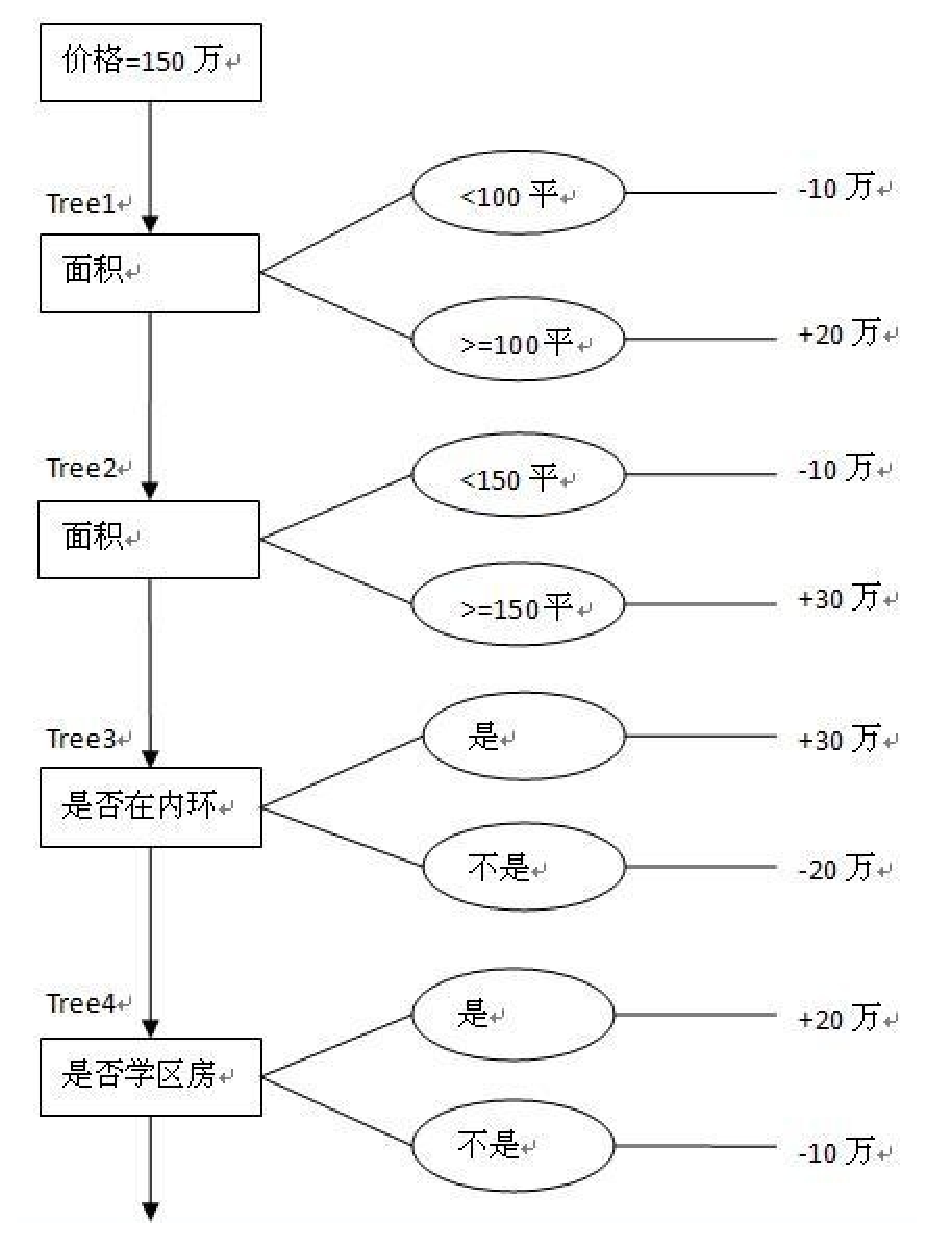
\includegraphics[width=0.85\textwidth,height=10cm]{figures/treelink.eps}
  \caption{商品房价格预测模型}\label{fig:treelink}
\end{figure}
对于新输入的样本,模型会赋予它一个初值(例子中初值设定为上海普通商品房价的均值150万),然后遍历每一棵决策树,每经过一棵树,都会对预测值进行调整修正,得到最后的预测结果:
\begin{equation}
    F(x) = F_0(x) + \sum\limits_{m=1}^M \beta_m h_m(x)
\end{equation}
比如,一个面积为120平米的内环非学区房,模型预测价格为:$150+20-10+30-10=180$万。
\end{example}

\subsection{排名问题}
\cite{busa2011ranking}和\cite{mohan2011web}使用逐点型排序学习方法,同序对型、序列型排序学习方法相比毫不逊色。\cite{busa2011ranking}在模型组合时引入序列型方法,取得不错的性能。\cite{mohan2011web}融合随机森林与GBDT的优点,使用随机森林模型初始化GBDT,不仅节省模型训练的时间,而且表现优于随机森林与GBDT算法。随机森林给了GBRT一个接近收敛的起始点,即使步长较小,也能很快结束迭代。

\chapter{聚类分析}
聚类分析是人类活动的一个重要内容,也是人类认知发展必然经历的一个过程。人类从孩童时期就在不断地完善潜意识下的分类模式,并逐渐掌握识别不同物理事物和抽象概念,如猫和狗、动物和植物、欢乐和痛苦等。所谓“物以类聚人以群分”,聚类是一个通过相似性关系划分抽象概念和物理对象的认知过程,有利于从复杂的信息结构中识别出规律性的数据分布特征,从而方便构建不同属性间的潜在关联。聚类分析是数据挖掘研究中一个非常活跃的研究课题,它不依赖人工标记数据揭示出数据内在关联与特征,已经成为机器学习、生物信息处理和市场分析等领域一个不可或缺的工具。

假设原始数据集$X=\{x_i\}_{i=1}^n$,$x_i\in \mathbb R^m$,聚类分析的目标是根据相似性关系将数据集划分至$K$个彼此不相交的子集(类簇或组),记作$\mathbb C=\{c_i\}_{i=1}^K$,则有
\[
    \bigcup\limits_{i=1}^K c_i = X,~~ c_s \cap c_t = \emptyset, \forall s\ne t = 1, 2,\ldots,K.
\]

\section{K-Means和K-Medoids}
K-Means算法从给定的K个初始簇心,根据数据点同簇心之间的距离,构造出K个簇类。一般地,K-Means算法是以迭代方式进行,在上一次构造的簇类上利用每个簇内所有数据点的均值选择新的簇心。K-Medoids算法与K-Means算法类似,不同之处在每次选取的质心,前者选中的必须是簇中的点。

\section{谱聚类}
传统聚类算法,如K-Means算法和K-Medoids算法,大多适用于凸球状样本空间,如果样本空间不是凸球状,则算法容易陷入局部最优。为了能够在任意形状的样本空间上做聚类分析,并使得聚类结果收敛于全局最优,研究人员设计出一种基于\textbf{谱图分割}(Spectral Graph Partition)的聚类算法:\textbf{谱聚类}(Spectral Clustering)。谱聚类算法以数据点为顶点,根据数据间的相似度连接数据顶点,构造一个无向加权图$G=(V, E)$,将聚类问题转化为谱图分割问题。在具体讨论谱聚类算法之前,我们先熟悉一下谱图分割算法及相关矩阵理论。

谱聚类算法计算出原始数据集$X$上的相似度矩阵(也称亲和矩阵)$A\in \mathbb R^{n\times n}$,根据一定的\textbf{连接规则}确定连接数据点的边,由此构造出含有$n$个顶点的无向加权图$G=(V, E)$,最终根据某种的\textbf{划分准则},可实现对$n$个数据顶点的聚类或分组。

谱聚类算法常用的连接规则有三种,对应地可以构造出三种不同的连接图:\textbf{全连接图}、\textbf{$\varepsilon-$近邻图}与\textbf{$K$近邻图},每一种连接图都对应一个边权矩阵$W\in \mathbb R^{n\times n}$。一般地,$W\ge 0$且$w_{ij}=0$表示节点$i$与$j$不相似,两个节点没有直接的连接通路。通常,数据相似度的选择依赖于数据空间的形状,比如凸球形的数据样本空间可以使用欧式距离定义相似性,对于非凸球形的样本空间最常见的是高斯核函数定义的相似性度量。
\begin{itemize}
  \item 如果直接使用数据相似度作为边的权值
        \[
            w_{ij}=a_{ij}, 1\le i,j \le n,
        \]
        我们可以构造出数据集$X$上的一个全连接图。
  \item 如果给定$\varepsilon>0$,并定义边的权值
        \[
            w_{ij}=\left\{
            \begin{array}{rl}
              a_{ij}, a_{ij}\ge \varepsilon,\\
              0, a_{ij}<\varepsilon,
            \end{array}
            \right.
        \]
        我们可以构造出数据集$X$上的一个$\varepsilon-$近邻图。
  \item 如果选定$K$值,连接各顶点的$K$个最近邻顶点,我们可以构造出$X$上的一个$K$近邻图。
\end{itemize}

我们下面从矩阵谱分析的角度分析谱聚类的理论基础,并在后续小节从图的划分角度分析它,建立谱聚类和矩阵论、谱图分割之间的紧密关系。
\subsection{谱分析}
假设$A\in \mathbb R^{n\times n}$是图$G$上顶点相似度矩阵,我们可以通过三种方法连接顶点,并构造对应图上边的权值矩阵$W\in \mathbb R^{n\times n}$。利用图上边的权值矩阵,我们可以计算各个顶点与其他顶点的连通度(Degree)。对于顶点$x_i$,其连通度定义为所有连接它和近邻顶点的边的权值之和,记作$d_i$,则有
\begin{equation}
    d_i = \sum\limits_{j=1}^n w_{ij},~~~D=\diag(d_1,\ldots,d_n)\in \mathbb R^{n\times n}.
\end{equation}
我们基于此构建三种类型的拉普拉斯矩阵(Graph Laplacian Matrix),它们是非标准化的拉普拉斯矩阵$L$、标准化对称的拉普拉斯矩阵$L_{\text{sym}}$和标准化随机游走的拉普拉斯矩阵$L_{\text{rw}}$:
\begin{eqnarray}
  L &=& D - W,\\
  L_\text{sym} &=& D^{-1/2} L D^{-1/2} = I - D^{-1/2} W D^{-1/2},\\
  L_\text{rw} &=& D^{-1} L = I - D^{-1} W.
\end{eqnarray}
由于拉普拉斯矩阵具有一些重要的基本性质,我们可以建立起矩阵谱系统和数据聚类的密切关联。
\begin{proposition}
非标准化拉普拉斯矩阵$L=D-W\in \mathbb R^{n\times n}$是对称的、半正定矩阵,对任意$f\in \mathbb R^n$都有
\[
    f^T L f = \frac{1}{2} \sum\limits_{1\le i,j\le n} w_{ij} (f_i-f_j)^2.
\]
它有$n$个非负实数特征值$\lambda_1\le \lambda_2 \le \cdots\le \lambda_n$,并且最小特征值$\lambda_1=0$,而其对应特征向量为$\mathbf 1$。
\end{proposition}

\begin{proposition}
假设$G$是一个无向图,边的权值非负,则矩阵$L$的零特征值的重数(Multiplicity)$K$与图$G$上独立连通子图的数目相同。如果记独立连通子图为$\{G_1,\ldots,G_K\}$,则零特征值对应的特征向量空间可由指标向量集$\{\mathbf 1_{G_1},\ldots,\mathbf 1_{G_K}\}$张成(Span)。
\end{proposition}
通过矩阵$L$的特征系统,利用其所有零特征值及对应特征向量可以直接将原始数据精确分组。一般地,原始数据存在大量的噪声干扰,非标准化的谱聚类算法计算拉普拉斯矩阵$L$ 的特征系统,固定或适应性地通过一个特征值阈值,选择出最小的$K$个特征值$\{\lambda_1,\ldots,\lambda_K\}$,利用对应特征向量$\{\alpha_1, \ldots, \alpha_K\}$ 将原始数据映射到一个低维空间
\[
    z_i = (\alpha_{1i}, \alpha_{2i}, \ldots, \alpha_{Ki})^T \in \mathbb R^K,~~~1\le i\le n
\]
在此低维数据集上运行K-Means聚类算法,对原始数据进行高效的近似分割。谱聚类算法存在一个明显的优势,它实际上不需显性的原始数据(维度不同或彼此异构),仅仅依赖于顶点之间的相似性关系,比其他聚类算法适用范围更广也更健壮。

\subsection{谱图分割}
目前,研究人员已经提出多种谱图分割方法,如最小割(Minimum Cut)、比率割(Ratio Cut)、标准割(Normalized Cut)等,将图的顶点分割成不相交的两个(Two-Way)或多个(K-Way)子图。我们将在后续章节逐一介绍它们。

假设图$G$可以被切割为$K$个彼此不相交的子图,分割准则是最小化被割边的权值之和,则有:
\begin{equation}\label{eq:mincut}
    \text{Cut}(c_1,\ldots, c_K) = \frac{1}{2} \sum\limits_{i=1}^K W(c_i,\bar c_i),
\end{equation}
其中,$\bar c_i$表示$c_i$的补集,$W(c_i,\bar c_i)$是$c_i$与$\bar c_i$间所有边的权值之和。由于最小割得到的子图分布可能极不均匀,出现部分子图为孤立点,其他子图所含数据点又太多。为此有人在最小割的基础上,提出改进的比率割:
\begin{equation}\label{eq:ratiocut}
    \text{RatioCut}(c_1,\ldots,c_K) = \frac{1}{2} \sum\limits_{i=1}^K \frac{W(c_i,\bar c_i)}{|c_i|} = \sum\limits_{i=1}^K \frac{\text{Cut}(c_i,\bar c_i)}{|c_i|},
\end{equation}
以及标准割:
\begin{equation}\label{eq:ratiocut}
    \text{NCut}(c_1,\ldots,c_K) = \frac{1}{2} \sum\limits_{i=1}^K \frac{W(c_i,\bar c_i)}{\text{vol}(c_i)} = \sum\limits_{i=1}^K \frac{\text{Cut}(c_i,\bar c_i)}{\text{vol}(c_i)},
\end{equation}
其中$|c|$表示$c$中所含顶点数目,$\text{vol}(c)=\sum\limits_{i\in c} d_i$表示$c$的容量。

\section{密度峰值聚类}
2014年,意大利国际高等研究院
\footnote{意大利国际高等研究院(\textit{it.} Scuola Internazionale Superiore di Studi Avanzati, \textit{en.} International School for Advanced Studies)创立于1978年,坐落于意大利北部城市里雅斯特(Trieste)。它是一所高级指导性学术研究中心,也是意大利第一所颁发博士学位的大学。它只在数学、物理及神经科学几个领域开展研究与教学,数学与神经科学在意大利排名第一,物理学排名第二,著名的国际理论物理中心就坐落在其校园内,声誉可与比萨高等师范学院(
\textit{it.} Scuola Normale Superiore di Pisa, \textit{en.} Advanced Normal School of Pisa)并肩。}
\href{http://people.sissa.it/~laio/index.html}{Alessandro Laio}教授的课题组提出一种基于密度峰值的高效聚类算法~\cite{rodriguez2014clustering},思想简明但效率和效果都很显著。它无需预先指定类簇数目,自动聚类时还能检测出异常点,一度成为年度聚类分析的热门话题。密度峰值聚类引入样本\textbf{局部密度}的概念,使得\textbf{每个类簇都是一个局部密度高地,而每个中心点都对应其类簇高地上的密度峰值,并为其近邻所环绕左右},故名\textbf{密度峰值聚类算法}。

\begin{figure}[ht]
  \centering
  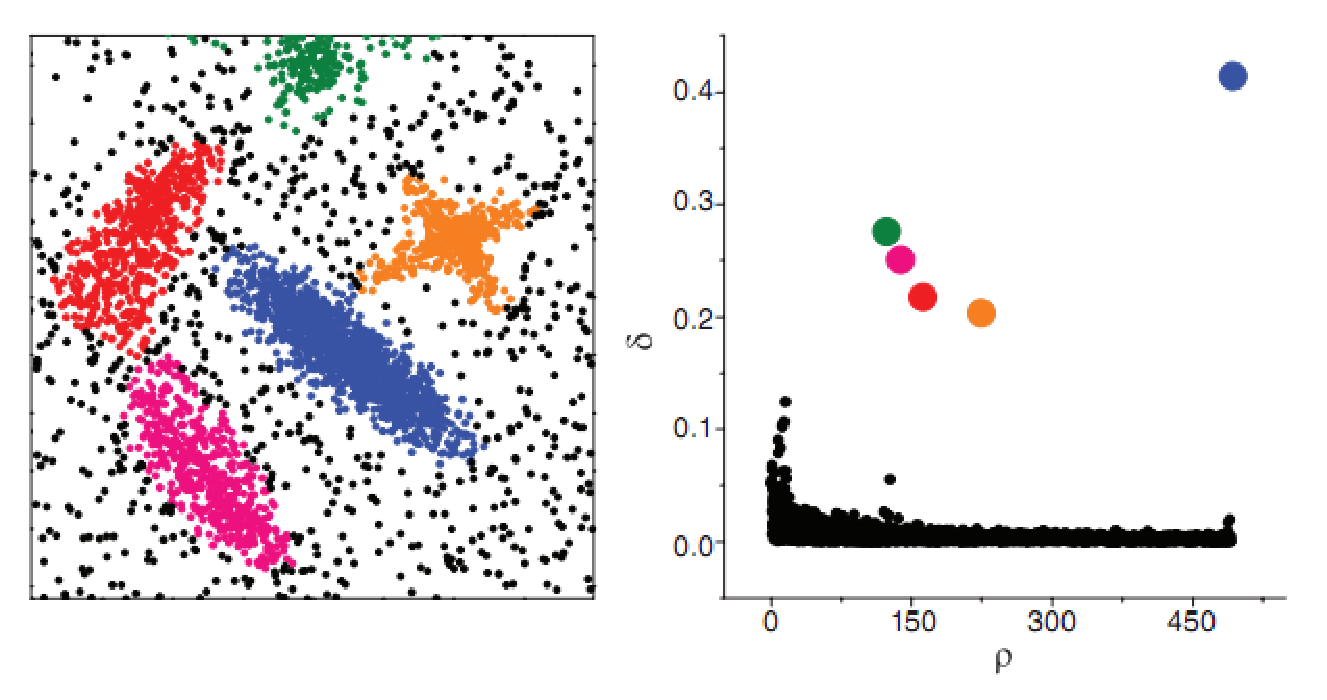
\includegraphics[width=0.8\textwidth, height=6cm]{figures/densitypeak_decisiongraph.eps}\\
  \caption{密度峰值聚类决策图~\cite{rodriguez2014clustering}}\label{fig:decisiongraph}
\end{figure}

密度峰值聚类算法依赖于两个指标:局部密度$\rho$、数据点与高密度近邻的最短距离$\delta$,后者依赖于前者以自动筛选类簇中心点。根据密度峰值聚类算法,数据点$x_i$ 的局部密度定义如下:
\begin{equation}\label{eq:localdensity}
    \rho_i = \sum\limits_{j=1}^n \chi(d_{ij}, d_c),~~~1\le i\le n,
\end{equation}
其中$d_c>0$是用户指定的截断距离,$d_{ij}$是$x_i$与$x_j$的空间距离,$\chi(\cdot)$是一个密度函数。一般地,距离$x_i$越近,对其密度的贡献越大,比如$\chi(d_{ij}, d_c) = e^{-d_{ij}/d_c}$。如果$\chi(d_{ij},d_c)=\ind(d_{ij} < d_c)$,则$x_i$的密度就是所有距离它在$d_c$范围内的近邻数目,计算密度时$d_c$范围外的点完全不予考虑。

密度峰值聚类算法将类簇内普通数据点视为其类簇中心点的随众,密度上低于中心点的局部密度,距离上相对其他高密度数据点中心数据点距离最近,每个类簇都是紧密围绕中心点而成的一个局部密度高地。一般地,聚类的显著特征是类簇内部紧密相联,而类簇之间则彼此分隔。
此外,算法还引入数据点与高密度近邻的最短距离
\begin{equation}
    \delta_i = \min\limits_{\rho_i < \rho_j} d_{ij},
\end{equation}
并对局部密度最大的数据点$\rho_i = \max\limits_{1\le j\le n} \rho_j$,定义其高密度最短距离
\begin{equation}
    \delta_i = \max\limits_{1\le j\le n} d_{ij}.
\end{equation}
如果以密度、高密度最短距离分别作横轴与纵轴,构建一个二维指标面板,则在面板右上角位置的点:密度高并且最短距离大,对应类簇的中心点。由此,指标面板可直接用作从数据集自动分离出类簇中心,实现自动分组的\textbf{决策图}(Decision Graph),如图\ref{fig:decisiongraph}。右侧决策图的右上角5个点对应五个类簇中心,其他点可依据各自高密度最近邻进行分组。从图\ref{fig:decisiongraph}和\ref{fig:dpcluster}可知密度峰值聚类算法性能优良、聚类准确。此外,密度峰值算法在分组时也存在一定的层次性,隐含不同类簇之间的蕴含关系,可以说它也是一个有效的\textbf{分层聚类方法}(Hierarchical Clustering Method)。
\begin{figure}[ht]
    \begin{minipage}[t]{\linewidth}
        \centering
          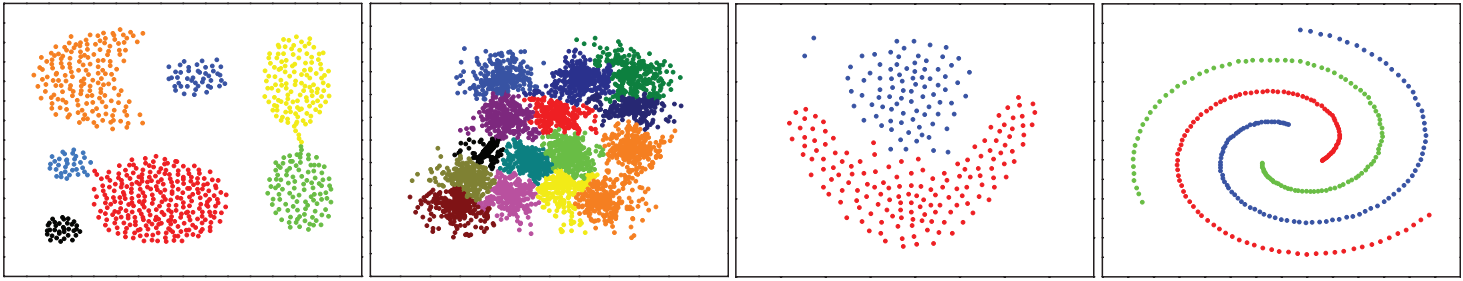
\includegraphics[width=0.95\textwidth,height=4cm]{figures/densitypeak_clustering}
    \end{minipage}
    \begin{minipage}[t]{\linewidth}
        \centering
          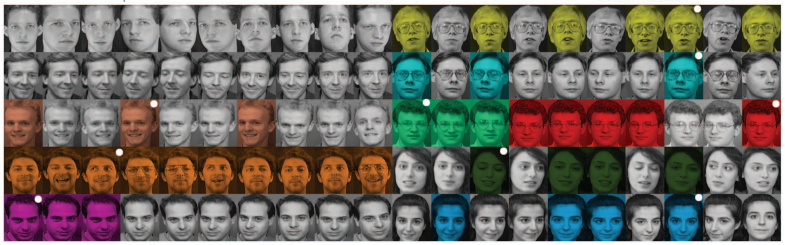
\includegraphics[width=0.95\textwidth,height=4cm]{figures/densitypeak_olivettiface}
    \end{minipage}
    \caption{经典人工数据集(上)与Olivetti人脸数据集(下)上密度峰值算法的性能~\cite{rodriguez2014clustering}}\label{fig:dpcluster}
\end{figure}

聚类算法在对不同数据分组时,可能存在可信度上的差异:有些可信度高,部分可信度差,后者很有可能就是异常点。为了能够从数据集中探测异常点,密度峰值聚类设法确定类簇间的模糊\textbf{边界}(Border),边界上的每个点与边界两侧的类簇中心的距离都在截断距离$d_c$ 范围之内。在确立类簇边界后,密度峰值聚类算法以边界上最高局部密度$\rho_c$作为检测异常点的阈值,当数据点的局部密度高于$\rho_c$,则认为此数据点的分组可信度高,称作\textbf{聚类核心
(Cluster Core)点},否则其可信度存疑,可以认定为\textbf{聚类光晕(Cluster Halo)点},即异常点。

\chapter{统计模型}
\section{EM算法}
EM(Expectation Maximization)算法是一种对缺失数据或者带有隐含变量的统计模型进行最大似然估计或最大后验估计的数值迭代算法\cite{dempster1977maximum}。本节简要介绍EM算法基本思想,并用它估计混合高斯模型的参数。

假设随机变量$X$的参数空间为$\theta$,则其的似然函数可表示为$P(X; \theta)$,根据最大似然估计法,我们可以通过最大化$P(X|\theta)$解出参数的似然估计值,等价地可以最大化其对数值:
\begin{equation}
  \max\limits_{\theta\in \Theta} L(\theta) = \log P(X; \theta).
\end{equation}
EM算法通过迭代的方式最大化对数似然函数,设当前参数估计值为$\theta_n$,则最大化对数似然函数即等价于解下面形式的目标函数:
\begin{equation}
  \max\limits_{\theta\in \Theta} L(\theta) - L(\theta_n) = \log P(X; \theta) - \log P(X; \theta_n).
\end{equation}
引入隐含变量$Z$,利用全概率公式$P(X; \theta) = \sum\limits_z P(X| z;\theta)P(z;\theta)$展开$L(\theta) - L(\theta_n)$,则有等式
\begin{equation}
\begin{array}{lcl}
  L(\theta) - L(\theta_n)  & = & \log\sum\limits_z P(X| z;\theta)P(z;\theta) - \log P(X;\theta_n) \\
  & = & \log\sum\limits_z P(X|z;\theta)P(z;\theta) \frac{P(z| X;\theta_n)}{P(z| X;\theta_n)} - \log P(X; \theta_n),
\end{array}
\end{equation}
由$\sum\limits_z P(z| X;\theta_n) = 1$与对数函数的凸性可知
\begin{eqnarray}
  L(\theta) - L(\theta_n) & \ge & \sum\limits_z P(z| X;\theta_n) \log \frac{P(X| z;\theta)P(z;\theta)}{P(z| X;\theta_n)} - \log P(X; \theta_n)\\
  & = & \sum\limits_z P(z| X;\theta_n) \log \frac{P(X|z;\theta)P(z;\theta)}{P(z| X;\theta_n)P(X;\theta_n)}\\
  & \triangleq & Q(\theta, \theta_n) - U(\theta_n)
\end{eqnarray}
其中,
\begin{eqnarray}
  &&Q(\theta, \theta_n) =  \sum\limits_z P(z|X;\theta_n) \log \big[P(X|z; \theta)P(z;\theta)\big],\\
  &&U(\theta_n) = \sum\limits_z P(z|X;\theta_n) \log \big[P(z|X; \theta_n)P(X;\theta_n)\big].
\end{eqnarray}
最大化$L(\theta)$可以通过其最大化$L(\theta) - L(\theta_n)$的一个下界近似趋近。既然$U(\theta_n)$与$\theta$完全无关,则等价于最大化$Q(\theta, \theta_n)$
\begin{equation}
    \max\limits_{\theta\in \Theta} \sum\limits_z P(z|X;\theta_n) \log P(X,z; \theta) = \sum\limits_z E_{z|X;\theta_n} \log P(X,z; \theta).
\end{equation}
至此,我们导出EM算法每次迭代所经历的两个基本步骤:
\begin{itemize}
  \item \textbf{E步骤}:$E_{z|X;\theta_n} \log P(X,z;\theta)$
  \item \textbf{M步骤}:$\max\limits_{\theta\in \Theta} E_{z|X;\theta_n} \log P(X,z;\theta)$
\end{itemize}

\subsection{高斯混合模型}
\textbf{高斯混合模型}(Gaussian Mixture Model,GMM),顾名思义是多个高斯模型的混合。假设混合模型$\Lambda$每个成员都是一个高斯模型,给定数据集$X=\{x_1, x_2,\ldots, x_n\}$,我们可以使用最大似然估计法估计模型的参数。假设数据集$X$所有样本独立同分布,可以构建对数似然函数
\begin{equation}
    L(X; \Lambda) = \sum\limits_i \log p(x_i; \Lambda),
\end{equation}
其中,$x_i\in \mathbb R^d, i = 1, 2, \ldots, n$。

混合模型是一个黑盒,我们的目标是剖解其结构,并利用EM算法估计各个成员参数。现在引入隐含随机变量$Z$,并根据全概率公式
\begin{equation}\label{eq:totalprob}
    p(x_i; \Lambda, p(z), z\in \mathbb Z) = \sum\limits_z p(z) p(x_i|z; \Lambda)
\end{equation}
改写对数似然函数
\begin{equation}
    L(X; \theta) = \sum\limits_i \log p(x_i; \theta) = \sum\limits_i \log \Big[\sum\limits_z p(z) p(x_i|z; \Lambda)\Big].
\end{equation}
其中,
\[\Lambda = \{\mu_z, \Sigma_z, z\in \mathbb Z\}, ~~\mu_z \in \mathbb R^d, \Sigma_z\in \mathbb R^{d\times d}\]
是混合模型中各个成员的均值向量与协方差矩阵,并且依赖于隐含随机变量$Z$,成员数目对应$\mathbb Z$的容量。新引入的概率分布$p(z),z\in \mathbb Z$表示各个成员在混合模型中的权重,且满足具有下面两个基本性质:
\begin{equation}
    0 < p(z) < 1,~~\sum\limits_z p(z) = 1.
\end{equation}
参数$\theta$对参数$\Lambda$与$p(z), z\in \mathbb Z$的组合定义:
\[\theta = \{\mu_z, \Sigma_z, p(z), z\in \mathbb Z\}.\]
根据混合模型的定义可知$x|z;\Lambda \sim N(\mu_z, \Sigma_z)$,则随机变量$x|z;\Lambda$对应的概率密度函数为
\begin{equation}
    p(x|z;\Lambda) = \frac{1}{(2\pi)^{d/2} |\Sigma_z|^{1/2}} \exp \Big\{-\frac{1}{2} (x-\mu_z)^T \Sigma_z^{-1} (x-\mu_z)\Big\}.
\end{equation}
假设混合模型的最大似然估计为$\hat \theta_{MLE}$,则有
\begin{equation}
    \hat \theta_{MLE} = \argmax\limits_{\theta\in \Theta} L(X; \theta) = \argmax\limits_{\theta\in \Theta} \sum\limits_i \log \Big[\sum\limits_z p(z) p(x_i|z; \Lambda)\Big].
\end{equation}

我们下面利用已知约束条件
\[
   0 < p(z) < 1,~~\sum\limits_z p(z) = 1,
\]
确定对数似然函数极值所对应的最优参数$\hat \Lambda$和$\hat p(z), z\in \mathbb Z$。由于约束条件只与参数$p(z)$相关,而参数$\Lambda$又不依赖于$p(z)$,故此可直接通过对数似然函数关于参数$\Lambda$的偏导解出对应的$\hat \Lambda$。当然,确定最优的$p(z)$,则相对复杂一些,要通过拉格朗日乘子法搜索。

我们现在利用拉格朗日乘子法搜索最优的$p(z), z \in \mathbb Z$:引入拉格朗日乘子$\lambda > 0$,构造拉格朗日函数
\begin{equation}
    \mathscr L = L(X; \theta) - \lambda (\sum\limits_z p(z) - 1).
\end{equation}
然后求关于$\lambda$与$p(z)$的偏导,并令它们为零,可以得到方程组
\begin{equation}\label{eq:partialarray}
    \left\{
        \begin{array}{lcl}
            \partial \mathscr L/\partial \lambda &=& 1 - \sum\limits_z p(z) = 0,\\
            \partial \mathscr L/\partial p(z) &=& \frac{\partial L(X; \theta)}{\partial p(z)} - \lambda = 0, ~~z\in \mathbb Z.
        \end{array}
    \right.
\end{equation}
在具体展开对数似然函数关于$p(z)$的偏导之前,可以看出:
\begin{equation}\label{eq:partialtheta}
    \frac{\partial L(X; \theta)}{\partial \theta} = \sum\limits_i \frac{1}{p(x_i; \theta)} \frac{p(x_i; \theta)}{\partial \theta},
\end{equation}
再根据全概率公式
\[p(x_i; \theta) = \sum\limits_z p(z) p(x_i|z; \Lambda),\]
我们可以推导$p(x_i; \theta)$关于$p(z)$的偏导:
\begin{equation}
    \frac{p(x_i; \theta)}{\partial p(z)} = p(x_i|z; \Lambda),
\end{equation}
将其代入式子\eqref{eq:partialtheta}可知
\[
\frac{\partial L(X; \theta)}{\partial p(z)} = \sum\limits_i \frac{p(x_i|z; \Lambda)}{p(x_i; \theta)}
    = \sum\limits_i \frac{p(x_i|z; \Lambda) p(z)}{p(x_i; \theta)} \frac{1}{p(z)}
    = \frac{1}{p(z)} \sum\limits_i p(z|x_i; \Lambda),
\]
再将其代入方程组\eqref{eq:partialarray},可以推得
\begin{equation}\label{eq:optimalpz}
    \hat p(z) = \frac{\sum\limits_i p(z|x_i;\Lambda)}{\sum\limits_z\sum\limits_i p(z|x_i;\Lambda)}
    = \frac{\sum\limits_i p(z|x_i;\Lambda)}{\sum\limits_i \sum\limits_z p(z|x_i;\Lambda)}
    = \frac{1}{n} \sum\limits_i p(z|x_i;\Lambda).
\end{equation}

我们继续从式子\eqref{eq:partialtheta}和全概率公式\eqref{eq:totalprob}出发,推导$p(x_i; \Lambda)$关于$\Lambda$的偏导:
\begin{equation}\label{eq:partiallambda}
    \frac{\partial L(X; \theta)}{\partial \Lambda}% = \sum\limits_i \frac{1}{p(x_i; \theta)} \frac{\partial p(x_i; \theta)}{\partial \Lambda}
   % = \sum\limits_i \frac{p(z)}{p(x_i; \theta)} \frac{\partial p(x_i|z;\Lambda)}{\partial \Lambda}
    = \sum\limits_i \frac{p(z) p(x_i|z;\Lambda)}{p(x_i; \theta)} \frac{\partial \log p(x_i|z;\Lambda)}{\partial \Lambda}
    = \sum\limits_i p(z|x_i;\Lambda) \frac{\partial \log p(x_i|z;\Lambda)}{\partial \Lambda}.
\end{equation}

根据变量$x_i|z;\Lambda$的概率密度函数,及其对数形式
\[
  \log p(x_i|z;\Lambda) = - \frac{d}{2} \log (2\pi) - \frac{1}{2} \log |\Sigma_z| - \frac{1}{2} (x_i - \mu_z)^T \Sigma_z^{-1} (x_i - \mu_z),
\]
其中协方差矩阵$\Sigma_z$是非奇异对称实矩阵,我们可以推导出$\log p(x_i|z;\Lambda)$关于均值向量$\mu_z$和协方差矩阵$\Sigma_z$的偏导函数:
\[
    \frac{\partial \log p(x_i|z;\Lambda)}{\partial \mu_z} %= \frac{1}{2} \Big[\Sigma_z^{-1} + \big(\Sigma_z^{-1}\big)^T\Big](x_i - \mu_z)
    = \Sigma_z^{-1} (x_i - \mu_z)
\]
将其代入等式\eqref{eq:partiallambda},再根据极值条件有:
\[
    \frac{\partial L(X; \theta)}{\partial \mu_z} = \sum\limits_i p(z|x_i;\Lambda) \Sigma_z^{-1} (x_i - \mu_z)
    = \Sigma_z^{-1} \sum\limits_i p(z|x_i;\Lambda) (x_i - \mu_z)
    = 0,
\]
从而解出最优解
\begin{equation}\label{optimalmuz}
    \hat \mu_z = \frac{\sum\limits_i p(z|x_i;\Lambda) x_i}{\sum\limits_i p(z|x_i;\Lambda)}.
\end{equation}

下面我们继续推导$\log p(x_i|z;\Lambda)$关于协方差矩阵$\Sigma_z$的偏导函数:
\begin{equation}\label{eq:partialsigmaz}
    \frac{\partial \log p(x_i|z;\Lambda)}{\partial \Sigma_z} = -\frac{1}{2} \Big[\frac{\partial \log |\Sigma_z|}{\partial \Sigma_z} + \frac{\partial (x_i - \mu_z)^T \Sigma_z^{-1} (x_i - \mu_z)}{\partial \Sigma_z}\Big]
    \triangleq -\frac{1}{2}\big[V_1(\Sigma_z) + V_2(\Sigma_z)\big]
\end{equation}
等式右侧第一部分$V_1(\Sigma_z)\in \mathbb R$是关于可逆矩阵的行列式求导,第二部分$V_2(\Sigma_z)\in \mathbb R$则涉及到矩阵迹的求导。在具体展开之前,我们先来看看矩阵求导的相关性质:
\begin{eqnarray}
  &&\frac{\partial \log |A|}{\partial A} = \big(A^{-1}\big)^T,~~|A|>0 \\
  &&\tr(ABC) = \tr(BCA) = \tr(CAB), ~~ABC\in \mathbb R \\
  &&\frac{\partial A^{-1} B}{\partial A} = -\big(A^{-1}\big)^T B \big(A^{-1}\big)^T, ~~|A|>0
\end{eqnarray}
利用这些性质,我们可以求$V_1(\Sigma_z)$与$V_2(\Sigma_z)$关于$\Sigma_z$的偏导函数:
\begin{eqnarray}
    \frac{\partial V_1(\Sigma_z)}{\partial \Sigma_z} &=& \big(\Sigma_z^{-1}\big)^T\\
    \frac{\partial V_2(\Sigma_z)}{\partial \Sigma_z} &=& \frac{\partial \tr\Big(\Sigma_z^{-1} (x_i - \mu_z)(x_i - \mu_z)^T\Big)}{\partial \Sigma_z}\\
    &=& -\big(\Sigma_z^{-1}\big)^T (x_i - \mu_z)(x_i - \mu_z)^T \big(\Sigma_z^{-1}\big)^T
\end{eqnarray}
同时代入式子\eqref{eq:partialsigmaz}与\eqref{eq:partiallambda},再根据极值条件有:
\[
    \frac{\partial L(X; \theta)}{\partial \Sigma_z} = -\frac{1}{2} \sum\limits_i p(z|x_i;\Lambda) \Big[\big(\Sigma_z^{-1}\big)^T -\big(\Sigma_z^{-1}\big)^T (x_i - \mu_z)(x_i - \mu_z)^T \big(\Sigma_z^{-1}\big)^T \Big]
    =0,
\]
从而解出最优解
\begin{equation}\label{optimalsigmaz}
    \hat \Sigma_z = \frac{\sum\limits_i p(z|x_i;\Lambda) (x_i - \mu_z)(x_i - \mu_z)^T }{\sum\limits_i p(z|x_i;\Lambda)}.
\end{equation}
综上可知最优解
\begin{eqnarray}
  &&\hat p(z) =  \frac{1}{n} \sum\limits_i \textcolor{red}{p(z|x_i;\Lambda)}\\
  &&\hat \mu_z = \frac{\sum\limits_i \textcolor{red}{p(z|x_i;\Lambda)} x_i}{\sum\limits_i p(z|x_i;\Lambda)}\\
  &&\hat \Sigma_z = \frac{\sum\limits_i \textcolor{red}{p(z|x_i;\Lambda)} (x_i - \mu_z)(x_i - \mu_z)^T }{\sum\limits_i p(z|x_i;\Lambda)}
\end{eqnarray}
都与$\textcolor{red}{p(z|x_i;\Lambda)}$紧密相关,而根据贝叶斯定理又有
\[
    p(z|x_i;\Lambda) = \frac{p(z)p(x_i|z;\Lambda)}{p(x_i;\theta)} = \frac{p(z)p(x_i|z;\Lambda)}{\sum\limits_z p(z) p(x_i|z;\Lambda)},
\]
其中
\[
    p(x_i|z;\Lambda) = \frac{1}{(2\pi)^{d/2} |\Sigma_z|^{1/2}} \exp \Big\{-\frac{1}{2} (x_i-\mu_z)^T \Sigma_z^{-1} (x_i-\mu_z)\Big\},
\]
可见参数最优解又决定了$\textcolor{red}{p(z|x_i;\Lambda)}$,彼此相互依赖。EM算法通过循环交替地使用E步骤与M步骤算出最优解。

EM算法引入的隐含随机变量在不同应用情景下具有不同的含义,比如聚类分析问题中的类别属性、词性分析问题中的单词词性等。
\section{概率隐语义分析}%Probabilistic Latent Semantic Analysis: pLSA
\section{隐含狄利克雷分布}%Latent Dirichlet Allocation: LDA

\section{最大熵模型}
最大熵模型(Maximum Entropy Model, MaxEnt)与隐马尔科夫模型(Hidden Markov Model, HMM)\cite{jurafsky1999speech}是自然语言处理(如词性标注、中文分词、句子边界识别、浅层句法分析及文本分类等\cite{berger1996maximum})和语音识别问题中得到广泛应用的两种统计模型。本节主要介绍最大熵模型,下一节重点介绍隐马尔科夫模型。

\subsection{最大熵原理}
1957年,物理学家Edwin Thompson Jaynes\cite{jaynes1957information1,jaynes1957information2}最早阐述了\textbf{最大熵原理}:
\begin{quote}
  \textit{Information theory provides a constructive criterion for setting up probability distributions on the basis of partial knowledge, and leads to a type of statistical inference which is called the maximum entropy estimate. It is least biased estimate possible on the given information; i.e., it is maximally noncommittal with regard to missing information.}
\end{quote}

最大熵原理是概率模型学习的一个准则,它对未知事物不做任何主观假设,在预测一个随机事件的概率分布时,在满足所有已知约束条件下,对未知情况不含任何主观偏见的结果是满足均匀概率分布,此时概率分布的信息熵做大,预测的风险也最小。根据最大熵原理推导的模型称作“最大熵模型”,比如投资学中“不要把所有的鸡蛋都放在一个篮子里”就是一种典型的最大熵策略:当出现不确定性时,就要保留各种可能性。

最大熵模型在形式上是最漂亮的统计模型,在实现上却是最复杂的模型之一,至今天为止,世界上能有效实现快速算法的人寥寥无几。第一个解决最大熵模型的优化算法是1972年John Darroch和Douglas Ratcliff联合提出的广义迭代尺度算法(Generalized Iterative Scaling, GIS)\cite{darroch1972generalized}。1989年,匈牙利著名数学家、信息论最高奖香农奖得主Imre Csiszar 从几何学角度详细分析最大熵模型\cite{csiszar1989geometric},并证明“对任何一组相容的信息,最大熵模型不仅存在,并且以指数函数的形式唯一存在”。由于GIS迭代算法效率低、复杂度高、稳定性差,在实际应用中鲜有人使用它。1997年,Della Pietra等人提出一种改进的迭代尺度算法IIS (Improved Iterative Scaling)\cite{della1997inducing},将最大熵模型训练所需时间降低了一两个数量级,成为当前最常用的最大熵模型优化算法。后来,Della Pietra兄弟二人离开IBM,退出学术圈转战金融界大显身手,加入当时籍籍无名的文艺复兴技术公司(Renaissance Technologies)。文艺复兴公司是数学家James Simons于1982年创立,已经发展为当今世界最成功的一家对冲基金公司。在金融市场,决定股票价格的因素成千上万,而最大熵方法正是建立能够同时满足所有不同条件的模型,文艺复兴技术公司的科学家们(包括Della Pietra兄弟)使用最大熵方法和其他先进的数学工具,建立量化的股票价格预测模型,获得巨大的成功。从1982年基金创立至今资产规模已经达到三百多亿美元,其净回报率高达平均每年34\%,远超股神巴菲特的旗舰公司——伯克希尔$\cdot$哈撒韦公司(Berkshire Hathaway)\cite{wu2012math}。

信息论提供了一种基于部分知识建立概率分布的构造性准则,由此而产生了一类统计推断(Statistical Inference)方法\footnote{统计推断方法是根据带随机性的观测数据(样本)以及问题的条件和假定(模型),而对未知事物作出的,以概率形式表述的推断。它是数理统计学的主要任务,其理论和方法构成数理统计学的主要内容。},即最大熵估计。在基于给定信息进行估计的所有方法中,最大熵估计属于最无偏见的一种,它对缺失的信息保留了最大的灵活性和不确定性\cite{jaynes1957information}。

根据最大熵原理,概率模型必须满足所有由已知事实构成的约束条件,并且在没有更多信息的条件下,其他不确定或未知的事件都是“等可能地发生”,而等可能的概率模型对应的熵最大。我们下面使用一个简单的实例介绍最大熵原理。
\begin{example}
假设随机投掷骰子,出现的点数$X$,则其可能取值为$\{1,2,\ldots,6\}$。对于某次投掷实验,估计各个点数出现的概率$P(X=1), P(X=2), \ldots, P(X=6)$。如果没有任何其他关于骰子的信息,根据最大熵对其点数出现的概率分布进行估计,则各个点数出现的概率相等$P(X=i)=1/6, i = 1, 2, \ldots, 6$。如果我们知道投掷骰子出现点数$1$和$6$的概率之和等于1/2,即概率分布的约束条件有两个:
\[P(X=1) + P(X=6) = 1/2, P(X=2) + P(X=3) + P(X=4) + P(X=5) = 1/2.\]
满足两个约束条件的概率分布有无穷多个,根据最大熵原理,可以认为出现点数1和点数6的概率是相等的,出现其他点数彼此也是等概率事件,即
\[P(X=1) = P(X=6) = 1/4, P(X=2) = P(X=3) = P(X=4) = P(X=5) = 1/8.\]
\end{example}

\subsection{最大熵模型}
假设分类模型是一个条件概率分布$P(Y|X)$,给定训练数据集$\{(x_1, y_1),(x_2,y_2),\ldots, (x_N, y_N)\}$,我们学习的目标是根据最大熵原理选择最佳的分类模型。从训练数据集,我们可以确定联合概率分布$P(X,Y)$的经验概率分布$\tilde{P}(X,Y)$、边际概率分布$P(X)$的经验概率分布$\tilde{P}(X)$,则有
\[\tilde{P}(x,y) = \frac{1}{N}C(x, y)\]
\[\tilde{P}(x) = \frac{1}{N}C(x)\]
其中,$C(x, y)$表示训练数据集中样本$(x,y)$出现的频数,$C(x)$ 表示训练数据集中输入$x$出现的频数。$N$表示训练样本容量。

为刻画已知事实,最大熵模型定义输入$x$与输出$y$的二值特征函数$f(x,y)$:当输入$x$与输出$y$之间存在某一事实关系,则$f(x,y)$ 取值1,否则取值0,其数学定义为
\[f(x,y) = \left\{
\begin{array}{ll}
    1, & x\text{与}y\text{存在某一事实},\\
    0, & \text{否则}.
\end{array}
\right.\]
如果给定训练数据集,则特征函数$f(x,y)$在训练集上的期望值$E_{\tilde P}(f)$定义如下:
\[E_{\tilde P}(f)=\sum \limits_{x,y} \tilde P(x,y) f(x,y)\]
其中,$\tilde P(x,y)$是样本$(x,y)$在数据集中的经验分布,可根据样本$(x,y)$在训练集上的频数进行计算。如果我们能够从数据集训练得到概率模型$P(y|x)$,则特征函数关于此概率模型的期望$E_P(f)$可写作:
\[E_P(f) = \sum\limits_{x,y} P(x, y) f(x,y) = \sum\limits_{x,y} \textcolor{red}{P(x)} P(y|x) f(x,y) = \sum\limits_{x,y} \textcolor{red}{\tilde P(x)} P(y|x) f(x,y)\]
其中,$\tilde P(x)$是样本输入$x$在数据集中的经验分布,与$\tilde P(x,y)$类似,可以从训练集中统计出相应频数并计算得到。我们对于输入真实的先验分布$P(x)$并不关心,从而直接使用数据集上的经验分布$\tilde P(x)$代替。如果概率模型能够充分刻画训练数据的所有信息,则可以认为特征函数的两种期望相等,即有
\begin{equation}
    E_P(f) = E_{\tilde{P}}(f).
\end{equation}
假设存在$n$个特征函数$f_i(x,y),i=1,2,\ldots,n$,刻画输入$x$与输出$y$的$n$种事实关系,它们就构成$n$个约束条件。

\begin{definition}[最大熵模型]
假设满足所有约束条件的概率模型集合为
\begin{equation}
   \mathcal P = \{P| E_P(f_i) = E_{\tilde{P}}(f_i), i = 1,2,\ldots,n\},
\end{equation}
则模型集合中条件熵
\begin{equation}
    H(P) = \sum\limits_x \textcolor{red}{P(x)} \Big(-\sum\limits_y P(y|x) \log P(y|x)\Big) = -\sum\limits_{x,y} \textcolor{red}{\tilde{P}(x)} P(y|x) \log P(y|x),
\end{equation}
最大的模型称作\textbf{最大熵模型}。
\end{definition}

\noindent 最大熵模型是如下带约束最优化问题
\begin{equation}\label{eq:maxent}
  \begin{array}{ll}
    \textit{max} & H(P) = -\sum\limits_{x,y} \tilde{P}(x)P(y|x) \log P(y|x)\\
    \textit{s.t.}& E_P(f_i) = E_{\tilde{P}}(f_i), i = 1,2,\ldots,n, \\
    & \sum\limits_y P(y|x) = 1,
  \end{array}
\end{equation}
的解,它等价于如下形式的最小化问题:
\begin{equation}
  \begin{array}{ll}
    \textit{min} & -H(P) = \sum\limits_{x,y} \tilde{P}(x)P(y|x) \log P(y|x)\\
    \textit{s.t.}&  E_{\tilde{P}}(f_i) - E_P(f_i)= 0, i = 1,2,\ldots,n, \\
    & \sum\limits_y P(y|x) = 1.
  \end{array}
\end{equation}
我们引入拉格朗日乘子$\lambda_0,\lambda_1,\lambda_2,\ldots, \lambda_n$,定义拉格朗日函数$L(P,\lambda)$:
\begin{equation}
    L(P,\lambda) = -H(P) + \lambda_0 \big(1-\sum\limits_{y} P(y|x)\big) + \sum\limits_i \lambda_i\big(E_{\tilde{P}}(f_i) - E_P(f_i)\big),
\end{equation}
将其转化为无约束最优化问题。
由于函数$L(P,\lambda)$是$P$的凸函数,原始问题$\min\limits_{P\in \mathcal P} \max\limits_{\lambda} L(P,\lambda)$与对偶问题$\max\limits_{\lambda} \min\limits_{P\in \mathcal P} L(P,\lambda)$的解等价,我们通过解对偶问题可以得到原始问题的解。对拉格朗日函数求关于$P(y|x)$ 的偏导,并令其为0,则有
\begin{equation}
    \frac{\partial L(P,\lambda)}{\partial P(y|x)} = \tilde{P}(x)\big[1 + \log P(y|x)\big] - \lambda_0 - \tilde{P}(x) \sum\limits_i \lambda_i f_i(x,y) = 0,
\end{equation}
由于$\tilde{P}(x)>0$,两边同除以$\tilde{P}(x)$,经过整理可得:
\begin{equation}
    P(y|x) = \exp\Big(\sum\limits_i \lambda_i f_i(x,y) + \frac{\lambda_0}{\tilde{P}(x)} - 1\Big),
\end{equation}
根据$\sum\limits_y P(y|x)=1$,可对其归一化处理,可得最大熵模型:
\begin{equation}
    P_\lambda(y|x) = \exp\Big(\sum\limits_i \lambda_i f_i(x,y)\Big)\frac{1}{Z_\lambda(x)},
\end{equation}
其中,$Z_\lambda(x)$是归一化因子:
\begin{equation}
    Z_\lambda(x) = \sum\limits_y \exp\Big(\sum\limits_i \lambda_i f_i(x,y)\Big).
\end{equation}
根据对偶理论,将最优概率模型$P_\lambda(y|x)$带入拉格朗日函数,最大化目标函数
\begin{equation}\label{eq:dualmaximum}
    \begin{array}{lcl}
        L(\lambda) & = &\sum\limits_{x,y} \tilde{P}(x) P_\lambda(y|x) \log P_\lambda(y|x) + \sum\limits_i \lambda_i \sum\limits_{x,y} \Big(\tilde P(x,y)-\tilde{P}(x) P_\lambda(y|x) \Big) f_i(x,y)\\
        & = & \sum\limits_{x,y} \tilde P(x,y) \sum\limits_i \lambda_i f_i(x,y) -\sum\limits_x \tilde P(x) \log Z_\lambda(x),
    \end{array}
\end{equation}
以确定最优模型参数$\lambda^*$。由于函数$L(\lambda)$是光滑凸函数,大多数优化算法,如梯度下降法、牛顿法、拟牛顿法、改进的迭代尺度(Improved Iterative Scaling, IIS)算法均适用,并搜索到$L(\lambda)$的全局最优解。我们下面介绍基于改进的迭代尺度算法搜索最大熵模型参数。

\subsection{参数优化 - IIS算法}
IIS算法通过迭代的方法搜索最优模型参数,假设当前参数向量为$\lambda=(\lambda_1,\lambda_2,\ldots,\lambda_n)^T$,只要在下次迭代时搜索到一个新的参数向量$\lambda+\delta=(\lambda_1+\delta_1, \lambda_2+\delta_2,\ldots, \lambda_n+\delta_n)^T$,使得目标函数$L(\lambda)$增大,依此不断更新参数,最终可以确定最优参数向量。当参数从$\lambda$更新至$\lambda+\delta$,目标函数$L(\lambda)$的变化量$\Delta L(\delta|\lambda) = L(\lambda+\delta) - L(\lambda)$:
\begin{equation}
    \begin{array}{lcl}
         \Delta L(\delta|\lambda) &=& \sum\limits_{x,y} \tilde P(x,y) \sum\limits_i \delta_i f_i(x,y)-\sum\limits_x \tilde P(x) \Big(\log Z_{\lambda+\delta}(x) - \log Z_\lambda(x) \Big)\\
        &=& \sum\limits_{x,y} \tilde P(x,y) \sum\limits_i \delta_i f_i(x,y)-\sum\limits_x \tilde P(x) \log \frac{Z_{\lambda+\delta}(x)}{Z_\lambda(x)}.
    \end{array}
\end{equation}
根据不等式$-\log \alpha \ge 1 - \alpha, \alpha > 0$,则有
\begin{equation}
    \begin{array}{lcl}
    \Delta L(\delta|\lambda) &\ge& \sum\limits_{x,y} \tilde P(x,y) \sum\limits_i \delta_i f_i(x,y)+\sum\limits_x \tilde P(x) (1-\frac{Z_{\lambda+\delta}(x)}{Z_\lambda(x)})\\
    & = & \sum\limits_{x,y} \tilde P(x,y) \sum\limits_i \delta_i f_i(x,y) + 1 - \sum\limits_x \tilde P(x) \sum\limits_y P_\lambda(y|x) \exp\Big(\sum\limits_i \delta_i f_i(x,y)\Big)\\
    & \triangleq & A(\delta|\lambda),
    \end{array}
\end{equation}
并确定目标函数变化量的一个下界$A(\delta|\lambda)$。如果我们可以搜索到一条使下界增加的路径,则目标函数$\Delta L(\delta|\lambda)$循此路径自然也会增加。由于$A(\delta|\lambda)$表达式中含有参数$\delta_i$的加和指数项,彼此相互依赖,不易同步更新所有维度的参数。我们改写下界函数$A(\delta|\lambda)$
\begin{equation}
    A(\delta|\lambda) = \sum\limits_{x,y} \tilde P(x,y) \sum\limits_i \delta_i f_i(x,y) + 1 - \sum\limits_x \tilde P(x) \sum\limits_y P_\lambda(y|x) \exp\Big(g(x,y) \sum\limits_i \frac{\delta_i f_i(x,y)}{g(x,y)}\Big),
\end{equation}
其中,
\[g(x,y) = \sum\limits_i f_i(x,y).\]
由于\[0\le \frac{f_i(x,y)}{g(x,y)} \le 1, \sum\limits_i \frac{f_i(x,y)}{g(x,y)} = 1,\]
根据Jensen不等式
\begin{equation}
    \exp\Big(\sum\limits_i \frac{f_i(x,y)}{g(x,y)} \delta_i \Big) \le \sum\limits_i \frac{f_i(x,y)}{g(x,y)} \exp \delta_i,
\end{equation}
再行放松下界函数$A(\delta|\lambda)$,可以得到它的一个下界
\begin{equation}
    \begin{array}{lcl}
    A(\delta|\lambda) &\ge& \sum\limits_{x,y} \tilde P(x,y) \sum\limits_i \delta_i f_i(x,y) + 1\\
    &&-\sum\limits_x \tilde P(x) \sum\limits_y P_\lambda(y|x) \sum\limits_i \frac{f_i(x,y)}{g(x,y)} \exp\big(\delta_i g(x,y)\big) \triangleq B(\delta|\lambda).
    \end{array}
\end{equation}
目前,最大化$L(\lambda + \delta) - L(\lambda)$近似等价于最大化$B(\delta|\lambda)$的问题,只要对$B(\delta|\lambda)$取关于$\delta_i$的导数并令其为0,可得等式:
\begin{equation}\label{eq:deltaroot}
    \frac{\partial B(\delta|\lambda)}{\partial \delta_i} = \sum\limits_{x,y} \tilde P(x,y) f_i(x,y) - \sum\limits_x \tilde P(x) \sum\limits_y P_\lambda(y|x) \sum\limits_i f_i(x,y) \exp\big(\delta_i g(x,y)\big)=0.
\end{equation}
如果$g(x,y)$是常数,则我们可以确定参数增量的解析解
\begin{equation}
    \delta_i = \frac{1}{g(x,y)} \log \frac{E_{\tilde P}(f_i)}{E_P(f_i)} = \frac{1}{g} \log \frac{E_{\tilde P}(f_i)}{E_P(f_i)}, i = 1, 2, \ldots, n.
\end{equation}
如果$g(x,y)$不是常数,我们可以使用牛顿法解出等式\eqref{eq:deltaroot}的根$\delta_i$,由此再更新参数向量$\lambda$
\[\lambda \leftarrow \lambda + \delta.\]
最大熵模型与逻辑回归模型形式相似,都属于概率模型,于是统称它们为\textbf{对数线性模型}(Log Linear Model)。

\subsection{模型参数最大似然估计}
我们下面考察最大熵模型的最大似然估计与对偶模型参数优化之间的关系,并证明两者等价。假设条件概率分布$P_\lambda(y|x)$是最大熵概率模型,我们通过最大化训练数据集上的对数似然函数
\begin{equation}
    L(\lambda) = \log \prod\limits_{x,y} P_\lambda(y|x)^{\tilde P(x,y)} = \sum\limits_{x,y} \tilde P(x,y) \log P_\lambda(y|x),
\end{equation}
确定参数$\lambda$的最大似然估计$\hat\lambda = \argmax\limits_\lambda L(\lambda)$。由于
\begin{equation}
    \begin{array}{lcl}
         L(\lambda) &=& \sum\limits_{x,y} \tilde P(x,y) \log P_\lambda(y|x)\\
         &=& \sum\limits_{x,y} \tilde P(x,y) \sum\limits_i \lambda_i f_i(x,y) - \sum\limits_{x,y} \tilde P(x,y) \log Z_\lambda(x)\\
         &=& \sum\limits_{x,y} \tilde P(x,y) \sum\limits_i \lambda_i f_i(x,y) - \sum\limits_{x} \tilde P(x) \log Z_\lambda(x),
    \end{array}
\end{equation}
它与式\eqref{eq:dualmaximum}完全相同,由此可以证明:最大熵模型参数在训练数据集上的极大似然估计与对偶问题优化等价。

\subsection{规则化模型}
由于通过式\eqref{eq:dualmaximum}得到的模型可能出现过拟合,我们给目标函数添加一个正则化项\cite{huang2010iterative},以控制模型的复杂度
\begin{equation}
    L(\lambda) = \sum\limits_{x,y} \tilde P(x,y) \sum\limits_i \lambda_i f_i(x,y) - \sum\limits_{x} \tilde P(x) \log Z_\lambda(x) + \frac{1}{2\sigma^2} \sum\limits_i \lambda_i^2,
\end{equation}
其中,$\sigma>0$是正则化因子,添加了正则化项的目标函数是严格的凸函数。

\section{隐马尔科夫模型}\label{sec:hmm}
\textbf{隐马尔科夫模型}(Hidden Markov Model,HMM)描述由隐含未知参数的马尔科夫链随机生成观测序列的过程,属于生成模型(Generative Model)\footnote{机器学习模型通常可以划分为判别模型(Discriminative Model)和生成模型。在典型的机器学习问题中,常常会给定输入$X$ 和输出$Y$,通过寻找$X$ 和$Y$之间的关系进行预测。判别模型通过给定$X$,寻找$Y$ 的规律(如分类器),而生成模型试图确定$X$ 和$Y$同时满足何种规律。从概率的角度来看,判别模型对应着条件概率分布,而生成模型对应于联合概率分布。}。
HMM是对马尔科夫模型的一种扩充,20世纪60年代末70 年代初Leonard Baum等人\cite{baum1966statistical,baum1967inequality,baum1968growth,baum1970maximization} 的研究工作奠定了HMM的理论基础。70年代,卡内基梅隆大学的James Baker\cite{baker1975dragon}和IBM的Frederick Jelinek等人\cite{jelinek1975design}将其应用到语音识别问题。后来,计算语言学家用它来处理英语文本的词性标注(Part-of-Speech Tagging, POST),并取得极大成功。现在,HMM已经广泛应用于语音识别、自然语言处理、生物信息、模式识别、信息抽取等领域\cite{li2012statlearning}。

\begin{definition}[马尔科夫链]
假设$\mathcal S$是由有限个状态组成的集合,如果随机序列$X$在$t+1$时刻所处的状态$s_{t+1}\in \mathcal S$只与它在$t$时刻的状态$s_t\in \mathcal S$ 有关,而与它$t$时刻之前的所有状态均无关,即满足
\[
    P(s_{t+1}|s_t, s_{t-1},\ldots) = P(s_{t+1}|s_t),
\]
则称随机序列$X$构成一阶\textbf{马尔科夫链}(Markov Chain),随机序列在不同时刻的状态序列构成一个\textbf{随机游走}(Random Walk)路径。
\end{definition}

假设$\mathcal S=\{1,2,\ldots,n\}$表示有限个状态索引表,$O=\{1,2,\ldots,m\}$表示有限个观测值或输出符号索引表,$X=\{x_1,x_2,\ldots,x_T\}$表示一个长度为$T$的状态序列,$Z=\{s_1,s_2,\ldots,s_T\}$为观测序列$X$对应的潜在状态序列,隐马尔科夫模型可以使用一个三元组$\Theta=(A, B, \pi)$表示,其中$A$ 表示状态转移矩阵$A= (a_{ij})_{n\times n}$
\[
    a_{ij} = P(s_{t+1} = j|s_t = i),1\le i,j\le n,
\]
$B$表示观测值或输出符号的概率分布矩阵$B=(b_{jk})_{n\times m}$
\[
    b_{jk} = P(x_t = k|s_t = j),1\le j\le n,1\le k\le m,
\]
$\pi$是初始状态概率分布$\pi = (\pi_1,\pi_2,\ldots,\pi_n)^T$
\[
    \pi_i = P(s_1=i),1\le i\le n.
\]
隐马尔科夫模型是一个双重随机过程,一重随机过程无法直接观测,只能通过状态转移矩阵描述,另一重随机过程输出可以观察到的观测值或输出符号,通过输出符号的概率分布矩阵描述。实际上,隐马尔科夫模型假设随机序列满足\textbf{齐次马尔科夫性}和\textbf{观测独立性}。所谓齐次马尔科夫性表示隐马尔科夫链在任意时刻$t+1$的状态只依赖于前一时刻$t$的状态,与时刻$t$、其他时刻马尔科夫链的状态和观测值都无关,即
\[
    P(s_{t+1}|s_t) = P(s_{t+1}|s_t,x_t,s_{t-1},x_{t-1},\ldots,s_1,x_1).
\]
观测独立性假设任意时刻$t$的观测只依赖于时刻$t$马尔科夫链的状态,与其他时刻马尔科夫链的观测值与状态均无关,即
\[
    P(x_t|s_1,x_1, \ldots,s_t,x_t,s_{t+1},x_{t+1},\ldots) = P(x_t|s_t).
\]

隐马尔科夫模型可用以解决三类问题:\textbf{评估问题}、\textbf{解码问题}和\textbf{学习问题}。所谓评估问题是指给定模型参数$\Theta=(A,B,\pi)$和\textbf{观测序列}(Observation Sequence)$X=\{x_1,x_2,\ldots,x_T\}$,有效估算出隐马尔科夫模型生成观测序列$X$的概率$P(X;\Theta)$。解码问题是指给定模型参数$\Theta$ 和\textbf{观测序列}(Observation Sequence)$X$,搜索最有可能生成观测序列$X$的隐含\textbf{状态序列}(State Sequence)$Z=\{s_1,s_2,\ldots,s_T\}$。学习问题则是使用最大似然估计确定模型参数。我们下面就这三个问题介绍隐马尔科夫模型的原理。

\subsection{评估问题:Forward-Backward算法}
隐马尔科夫模型可以从状态指标集$\mathcal S=\{1,2,\ldots,n\}$中产生$n^T$个长度为$T$的潜在状态序列$Z=\{s_1,s_2,\ldots,s_T\}$,每个潜在的状态序列都可能产生给定的观测序列$X=\{x_1,x_2,\ldots,x_T\}$。评估问题在模型参数$\Theta=(A,B,\pi)$和观测序列$X$的基础上,估算出模型生成观测序列$X$的概率$P(X;\Theta)$,根据全概率公式有
\[
\begin{array}{lcl}
    P(X;\Theta) &=& \sum\limits_Z P(X|Z;\Theta) P(Z;\Theta) \\
    &=& \sum\limits_Z P(x_1,x_2,\ldots,x_T|s_1,s_2,\ldots,s_T;\Theta) P(s_1,s_2,\ldots,s_T;\Theta)\\
    &=& \sum\limits_Z \big[P(x_1|Z;\Theta) \prod\limits_{i=1}^{T-1} P(x_{i+1}|x_1,\ldots,x_i,Z;\Theta)\big] \big[P(s_1;\Theta) \prod\limits_{i=1}^{T-1} P(s_{i+1}|s_1,\ldots,s_i;\Theta)\big],
\end{array}
\]
根据隐马尔科夫模型的基本假设可知
\[
    P(x_{i+1}|Z, x_1,\ldots,x_i;\Theta) = P(x_{i+1}|s_{i+1};\Theta),~~~P(s_{i+1}|s_1,\ldots,s_i;\Theta) = P(s_{i+1}|s_i;\Theta),
\]
则有
\[
\begin{array}{lcl}
    P(X;\Theta) &=& \sum\limits_Z \prod\limits_{i=1}^{T-1} \big[P(x_i|s_i;\Theta)P(x_{i+2}|x_i;\Theta)\big] P(x_T|s_T;\Theta) P(s_1;\Theta)\\
    &=&\sum\limits_Z \pi_{s_1} \prod\limits_{i=1}^{T-1} [a_{s_i,s_{i+1}} b_{s_i,x_i}]b_{s_T,x_T}.
\end{array}
\]
计算这个概率分布需要$(2T-1)n^T$次乘法运算,$n^T-1$次加法运算,计算量相当大。如果深入概率分布$P(X;\Theta)$的计算公式可以发现,对于每个可能的状态序列$Z$,都存在很多重复计算。为此,Leonard Baum等人改进原始计算方法,在部分观测数据上定义局部概率分布,通过递推的方式逐步完成对$P(X;\Theta)$的计算。我们在下文分别介绍两种高效的计算方法:\textbf{前向算法}(Forward Algorithm)和\textbf{后向算法}(Backward Algorithm)。

前向算法利用时刻$t$之前所有观测数据,定义前向变量$\alpha_t(i)=P(x_1,x_2,\ldots,x_t, s_t=i;\Theta)$。它表示给定模型参数$\Theta$,时刻$t$的状态为$s_t$,部分序列观测值为$x_1,x_2,\ldots,x_t$的联合概率。显然,$\alpha_1(i)=P(x_1,s_1=i;\Theta)=\pi_i b_{i,x_1}$,根据基本假设,可以推导出相邻时刻前向变量$\alpha_{t+1}(i)$ 和$\alpha_t(i)$之间的关系
\begin{equation}
\begin{array}{lcl}
    \alpha_{t+1}(i) &=& P(x_1,\ldots,x_t,x_{t+1},s_{t+1} = i;\Theta)\\
    &=& \sum\limits_{j\in \mathcal S} P(x_1,\ldots,x_t,s_t=j,x_{t+1},s_{t+1} = i;\Theta)\\
    &=& \sum\limits_{j\in \mathcal S} P(x_{t+1}|x_1,\ldots,x_t,s_t=j,s_{t+1} = i; \Theta) P(x_1,\ldots,x_t,s_t=i,s_{t+1} = j; \Theta)\\
    &=& \sum\limits_{j\in \mathcal S} P(x_{t+1}|s_{t+1} = i; \Theta) P(s_{t+1} = i|x_1,\ldots,x_t,s_t=j;\Theta)P(x_1,\ldots,x_t,s_t=j; \Theta)\\
    &=& \sum\limits_{j\in \mathcal S} b_{i,x_{t+1}} P(s_{t+1} = i|s_t=j; \Theta) \alpha_t(j)\\
    &=& \sum\limits_{j\in \mathcal S} b_{i,x_{t+1}} a_{ji} \alpha_t(j) = \big[\sum\limits_{j\in \mathcal S} a_{ji} \alpha_t(j)\big]b_{i,x_{t+1}},
\end{array}
\end{equation}
我们下面利用所有前向变量推导和估算模型生成观测序列$X$的概率$P(X;\Theta)$
\begin{equation}
\begin{array}{lcl}
    P(X;\Theta)&=&P(x_1,x_2,\ldots,x_T;\Theta)\\
    &=&\sum\limits_{i\in \mathcal S} P(x_1,x_2,\ldots,x_T,s_T=i;\Theta)\\
    &=&\sum\limits_{i\in \mathcal S} \alpha_T(i).
\end{array}
\end{equation}
估算需要$n(n+1)(T-1)+n$次乘法运算,$n(n-1)(T-1)+n$次加法运算。

\begin{algorithm}[htbp]
\caption{前向算法(Forward Algorithm)}
\begin{algorithmic}
    \REQUIRE ~~模型参数$\Theta=(A,B,\pi)$,观测序列$X=\{x_1,x_2,\ldots,x_T\}$
    \begin{enumerate}[1.]
        \item 初始化前向变量$\alpha_1(i)=\pi_i b_{i,x_1}$,$i\in \mathcal S$
        \FOR{$t = 1, 2, \ldots, T-1$}
        \item 计算前向变量$\alpha_{t+1}(i)=\big[\sum\limits_{j\in \mathcal S} a_{ji} \alpha_t(j)\big]b_{i,x_{t+1}},~~~i\in \mathcal S.$
        \ENDFOR
    \end{enumerate}
    \ENSURE ~~估算模型生成观测序列$X$的概率$P(X;\Theta)=\sum\limits_{i\in \mathcal S} \alpha_T(i).$
\end{algorithmic}
\end{algorithm}

后向算法利用时刻$t$之后的所有观测数据,定义后向变量$\beta_t(i)=P(x_{t+1},x_{t+2},\ldots,x_T|s_t=i;\Theta)$。它表示给定模型参数$\Theta$,时刻$t$的状态为$s_t$,部分序列观测值为$x_1,x_2,\ldots,x_t$的条件概率。对任意$i\in \mathcal S$,后向算法初始化时刻$T$的后向变量$\beta_T(i)=1$,由此可以推导出其他时刻的后向变量
\begin{equation}
\begin{array}{lcl}
    \beta_t(i) &=& \sum\limits_{j\in \mathcal S} P(x_{t+1},x_{t+2},\ldots,x_T,s_{t+1}=j|s_t=i;\Theta)\\
    &=& \sum\limits_{j\in \mathcal S} P(x_{t+2},\ldots,x_T|\textcolor{red}{s_{t+1}=j,x_{t+1},s_t=i};\Theta)P(s_{t+1}=j,x_{t+1}|s_t=i;\Theta)
\end{array}
\end{equation}
由于$P(s_{t+1}=j,x_{t+1}|s_t=i;\Theta) = P(x_{t+1}|s_{t+1}=j,s_t=i;\Theta)P(s_{t+1}=j|s_t=i;\Theta)$,根据基本假设则有
$P(x_{t+1}|s_{t+1}=j,s_t=i;\Theta)=P(x_{t+1}|s_{t+1}=j;\Theta)=b_{j,x_{t+1}}$,$P(s_{t+1}=j|s_t=i;\Theta)=a_{ij}$,所以
\begin{equation}\label{eq:backwardbeta}
    \beta_t(i)=\sum\limits_{j\in \mathcal S} \beta_{t+1}(j) b_{j,x_{t+1}} a_{ij}.
\end{equation}
我们下面利用所有后向变量推导和估算模型生成观测序列$X$的概率$P(X;\Theta)$
\begin{equation}
\begin{array}{lcl}
    P(X;\Theta)&=&P(x_1,x_2,\ldots,x_T;\Theta)\\
    &=&\sum\limits_{i\in \mathcal S} P(x_1,x_2,\ldots,x_T,s_1=i;\Theta)\\
    &=&\sum\limits_{i\in \mathcal S} P(x_2,\ldots,x_T|x_1,s_1=i;\Theta)P(x_1,s_1=i;\Theta)\\
    &=&\sum\limits_{i\in \mathcal S} \beta_1(i) b_{i,x_1} \pi_i.
\end{array}
\end{equation}
估算需要$n(n+1)(T-1)+2n$次乘法运算,$n(n-1)(T-1)+n$次加法运算。

\begin{algorithm}[htbp]
\caption{后向算法(Backward Algorithm)}
\begin{algorithmic}
    \REQUIRE ~~模型参数$\Theta=(A,B,\pi)$,观测序列$X=\{x_1,x_2,\ldots,x_T\}$
    \begin{enumerate}[1.]
        \item 初始化后向变量$\beta_T(i)=1$,$i\in \mathcal S$
        \FOR{$t = T-1, T-2, \ldots, 1$}
        \item 计算后向变量$\beta_t(i)=\sum\limits_{j\in \mathcal S} \beta_{t+1}(j) b_{j,x_{t+1}} a_{ij},~~~i\in \mathcal S.$
        \ENDFOR
    \end{enumerate}
    \ENSURE ~~估算模型生成观测序列$X$的概率$P(X;\Theta)=\sum\limits_{i\in \mathcal S} \beta_1(i) b_{i,x_1} \pi_i.$
\end{algorithmic}
\end{algorithm}

\subsection{解码问题:Viterbi算法}
\subsection{学习问题:Baum-Welch算法}

\section{最大熵马尔科夫模型}
\noindent \textbf{最大熵马尔科夫模型}(Maximum Entropy Markov Model,MEMM),也称\textbf{条件马尔科夫模型}(Conditional Markov Model,CMM)是一类判别图模型(Discriminative Graphical Model),主要应用于自然语言处理,解决\textbf{词性标记}(Part-of-speech Tagging, POST)、信息抽取(Information Extraction)等问题。

\section{条件随机场}
\begin{definition}[概率无向图模型]
对于联合概率分布$P(X)$,可以通过一个无向图$G=(V,E)$来表示,则图$G$中每个结点对应一个随机变量,每条边对应两个随机变量之间的依赖关系。如果概率分布$P(X)$ 满足成对、局部或全局马尔科夫性,则称其为\textbf{概率无向图模型}(Probability Undirected Graphical Model),或\textbf{马尔科夫随机场}(Markov Random Field, MRF)\footnote{条件随机场是无向图上的一类判别模型,受限玻尔兹曼机(Restricted Boltzmann Machine)是无向图上的一类生成模型,\textbf{贝叶斯网络}(Bayesian Network)是一类有向无环图模型。}。
\end{definition}
马尔科夫随机场是马尔科夫链在多维空间上扩展,条件随机场(Conditional Random Fields, CRF)是一类判别型无向图模型,对于重叠的、非独立性特征具有良好的兼容性。线性链条件随机场(Linear Chain CRF)是一类特殊的CRF,实际上是无向图下的隐马尔科夫模型。如果说HMM是序列型朴素贝叶斯模型,线性链CRF就是序列型逻辑回归模型。

线性链CRF模型对应条件概率
\[
    P(z_1,\ldots,z_T|x_1,\ldots,x_T) = \frac{1}{\mathcal Z} \exp\bigg(\sum\limits_t \sum\limits_i \lambda_i f_i(z_t,z_{t+1},x_1,\ldots,x_T,t )\bigg),
\]
其中$\mathcal Z$是标准化因子,$f_i$是对应于时刻$t$的一个特征函数,$\lambda_i$是$f_i$的权重,$i=1,2,\ldots$。特征函数的确定是CRF的核心工作。

\chapter{集成学习}
集成学习(Ensemble Learning),最初称作委员会投票方法(Committee Voting Method),是一种新型机器学习框架,使用多个(通常是同质的)弱学习器解决同一个问题。比如在分类模型集成学习中,经常使用的弱学习器(分类器)是决策树分类器、神经网络分类器、贝叶斯分类器、K近邻分类器等,许多优秀的算法如AdaBoost,GBDT都属于集成学习算法。集成学习技术已经在行星探测、地震波分析、Web 信息过滤、生物特征识别等众多领域得到广泛应用,由于集成学习可以有效地提高学习系统的泛化能力,已经成为业界研究的热点课题,并被列为机器学习四大研究方向之首\cite{dietterich1997machine, ditterrich1997direction}。

\begin{figure}[htbp]
  \centering
  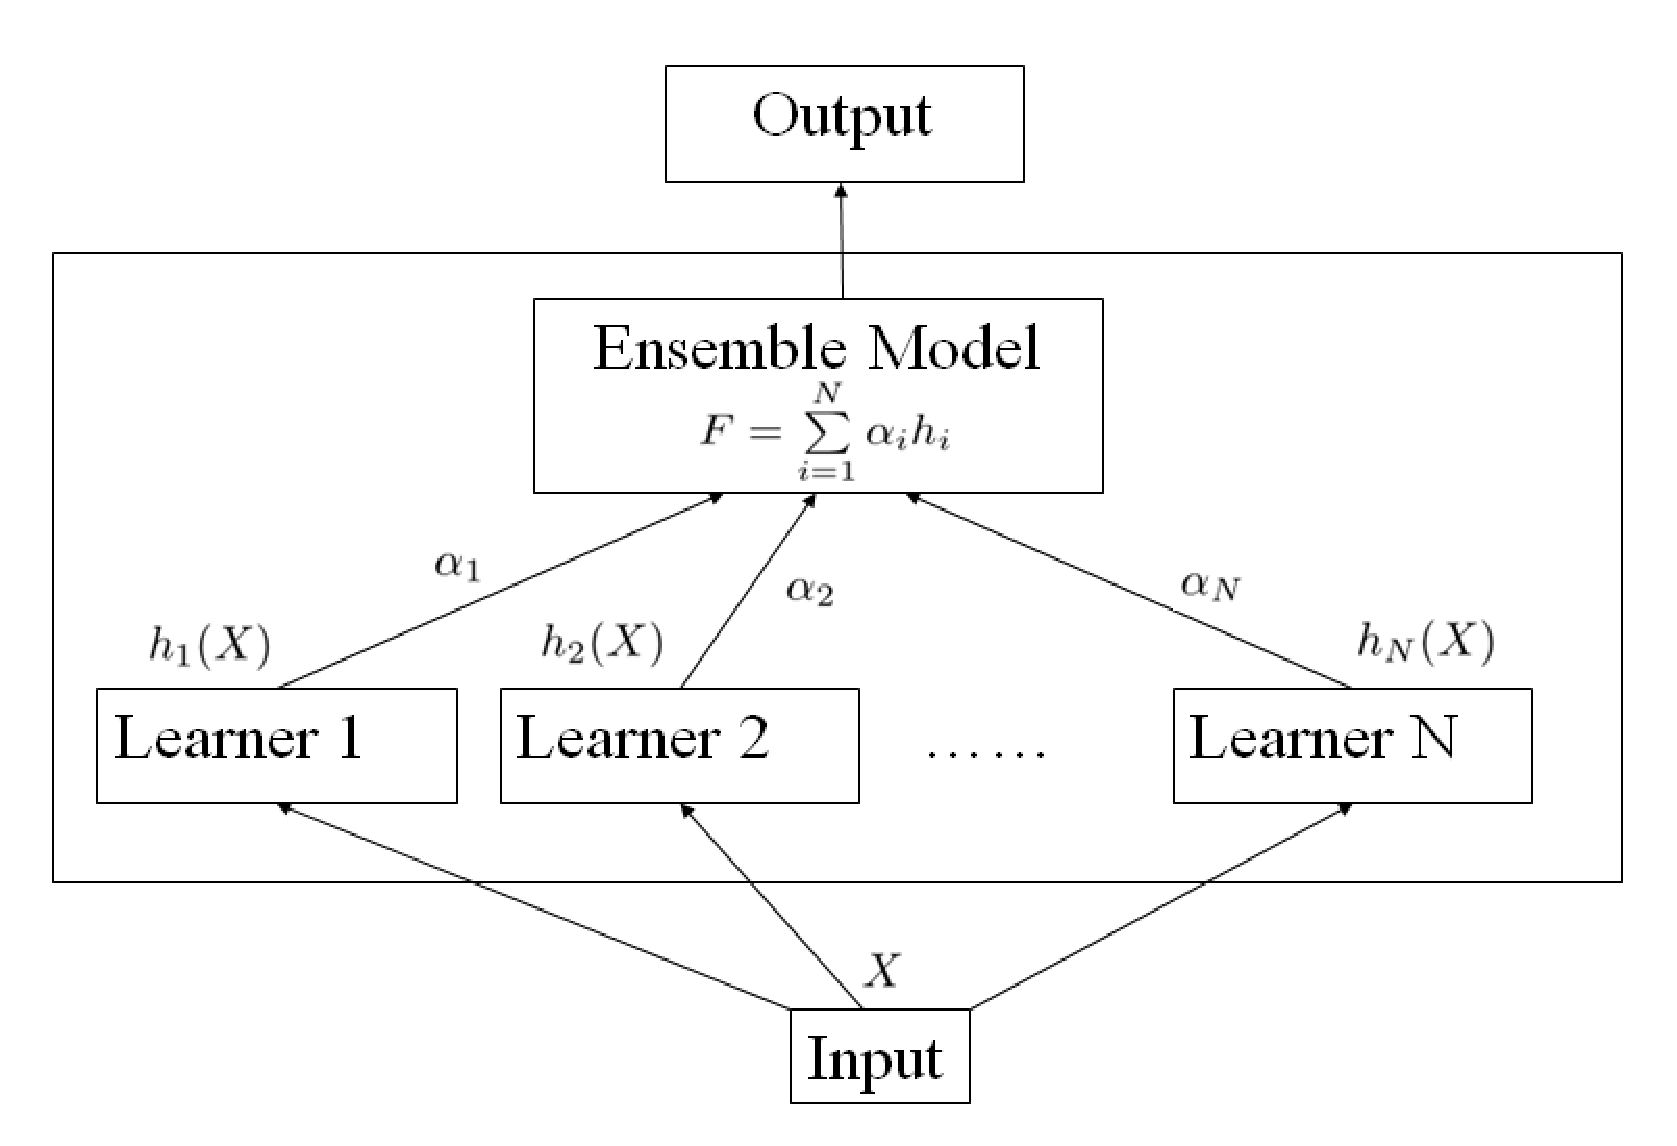
\includegraphics[width=0.6\textwidth,height=7cm]{figures/ensemblelearning.eps}\\
  \caption{集成学习框架}\label{fig:ensemblelearning}
\end{figure}

Thomas Dietterich\cite{dietterich2000ensemble}指出,集成学习有效可以归结于集成模型在统计、计算和模型表示三个方面的优势,认为集成模型能够有效地降低统计误差、优化误差和模型误差,那么构造出优良的集成模型自然水到渠成。

\begin{enumerate}[(1)]
  \item 统计的原因:一个学习算法就是从假设空间$\mathcal{H}$ 中寻找最佳的近似模型(假设),然而学习算法所使用的训练样本相对假设空间毕竟有限,假设空间中可能存在多个在训练集上精度相当的假设模型,构造集成模型要比选取单个模型更加明智,同时也免除了选择错误模型而带来的风险。
  \item 计算的原因:许多学习算法通常会陷于局部最优,通过增加训练样本,即便消除了统计误差,仍然不易找到全局最优的模型。每个假设模型实际上是从不同的初始点,不同的方向对真实函数的一种近似,集成模型的效果是大大降低单个模型的近似误差。
  \item 表示的原因:在实际应用中,也许假设空间$\mathcal{H}$ 中的任何假设都不能表示真实的函数$f$,那么通过加权形式集成的模型也就扩展了原始假设空间所表示的范围。
\end{enumerate}

在标准的监督学习问题中,给定训练数据集$S = \{x_i,y_i\}_{i=1}^n$,其中$x_i\in \mathbb{R}^m$是包含$m$个特征的样本,$y_i$表示样本的标记。假设样本特征$x$同样本标记$y$之间的真实关系是$y = f(x)$,或者说样本是从真实未知的分布$P(x,f(x))$ 中抽样得到。

假设当前学习的任务是训练一个分类器$h$,则分类器$h$就是未知函数$f$的一个假设。监督学习的目标是从训练数据集中学习出最佳模型$h\in \mathcal H$,从而使得损失函数的期望值最小:
\[
    h = \argmin\limits_{g\in \mathcal H} \mathbb E_{y,x} L(y,g(x))
\]
由于客观条件的限制,最终训练得到的模型还是会存在下面三种类型的误差(1)统计误差:由于真实函数未知,模型训练使用的训练集只能通过采样构建,并基于它最小化经验风险。(2)优化误差:优化损失函数的算法通常确定的是局部最优解,从而产生与全局最优解不一致的误差。(3)模型误差:监督学习建立在给定形式的模型上,或基于一定的先验概率,在模型空间的子空间中搜索,从而产生结构性的模型误差。集成学习的有效性分析,实际上就是分析集成模型降低统计误差、优化误差或模型误差的能力。

\ornamento
\section{多样性}\label{sec:diverisity}
假设集成分类器$F$包含$m$个基本分类器$\{h_i\}_{i=1}^m$,集成分类器的预测精度高于单个分类器的充分必要条件\cite{hansen1990neural}是:对于新的输入样本,单个分类器的预测精度要比随机猜测的高(Accurate),基本分类器间的预测误差具有差异性(Diverse)\cite{dietterich2000ensemble}。有研究表明,预测误差差异性的增加能够改善集成模型的性能:对于相同的输入,如果所有基本模型都给出相似的预测结果,则集成模型的泛化误差大于基本模型泛化误差的加权平均值;如果基本模型的预测误差存在较大的差异性,则集成模型的泛化误差远小于基本模型泛化误差的加权平均值。

A necessary condition for an ensemble to be more accurate than any of its individual members, is that the classifiers are accurate and diverse\cite{hansen1990neural}. An accurate classifier does better than random guessing on new examples. Two classifiers are diverse if they make different errors on new examples. There are several ways to introduce diversity: by \textbf{manipulating the training set} (by changing the weight of the examples\cite{breiman1996bagging,freund1996experiments} or by \textbf{changing the attribute values of the examples} \cite{breiman1999using}), or by \textbf{manipulating the learning algorithm itself} \cite{dietterich2000ensemble}.

目前,常见的增加集成模型误差多样性的方法包括:使用不同的训练集合(行采样、列采样)、使用不同类型的基本模型(模型结构、参数、初始化方式),整体而言可以分为同构(Homogeneous)与异构(Heterogeneous)模型两种。比如,Bagging、Boosting集成的基本模型是同构模型,Stacking集成的基本模型是异构模型。

Carbonell与Goldstein\cite{carbonell1998use}认为,评价信息检索的指标不仅要关注“检索相关性”(Query Relevance),还要考虑“信息新颖度”(Information Novelty)。他们引入“间隔相关性”(Marginal Relevance)的概念,兼顾相关性与新颖度,并充分考虑用户的个性化需求,通过灵活设置权衡参数,反映对二者的偏好程度。间隔相关性是相关性与新颖度的线性组合,选择备选文档的原则是最大化间隔相关性:
\begin{equation}\label{eq:mmr}
    \mathrm{MMR} = \argmax\limits_{d_i\in D\setminus S}\Big\{\lambda sim_1(d_i, q) - (1-\lambda) \max\limits_{d_j\in S}sim_2(d_i, d_j)\Big\}
\end{equation}
其中,$D$是文档集合,$S$代表已经选择的文档集,$q$表示检索词,$q_i,q_j$表示文档,$sim_1,sim_2$分别是文档-检索词相关性、文档-文档相似性的度量,$\lambda\in [0,1]$反映了对相关性偏好程度,比如当$\lambda=1$时,则仅仅以相关性为选择标准,当$\lambda = 0$,则新颖度是选择文档的主要依据。分析可以发现,如果备选文档同检索词相关程度越高,备选文档同已选文档之间的相似程度越低,则MMR越大。

由于精度-多样性两难问题(Accuracy-Diversity Dilemma),只有深入研究多样性同模型精度之间的密切关系,才能通过恰当的权衡获得最佳的性能。对此,多人已经作出深刻的分析\cite{cunningham2000diversity,kuncheva2003measures,tsymbal2005diversity}。 不同类型的多样性对于集成学习的影响也不同,
\cite{kuncheva2002experimental}中介绍了九种多样性度量,\cite{kuncheva2003measures}介绍了十种多样性度量。

\section{集成误差}
1992年,Stuart Geman等人\cite{geman1992neural}证明集成模型的预测误差可以分解为偏差、方差两部分(Bias-Variance分解)
\begin{equation}\label{eq:biasvariancedec}
    E (F - y)^2 = (E(F) - y)^2 + E(F- E(F))^2= \beta_F^2 + \sigma_F^2
\end{equation}
其中,$y$表示含有噪声的相应变量期望值,$F$表示集成模型,$\beta_F^2$表示它的预测偏差,$\sigma_F^2$表示集成模型的预测方差。图\ref{fig:bias-variance}形象解释了偏置与方差两个概念,偏置描述训练模型逼近真实模型的程度,而方差则反映训练模型忽略真实信号,学习随机事物的程度。

\begin{figure}[htbp]
  \centering
  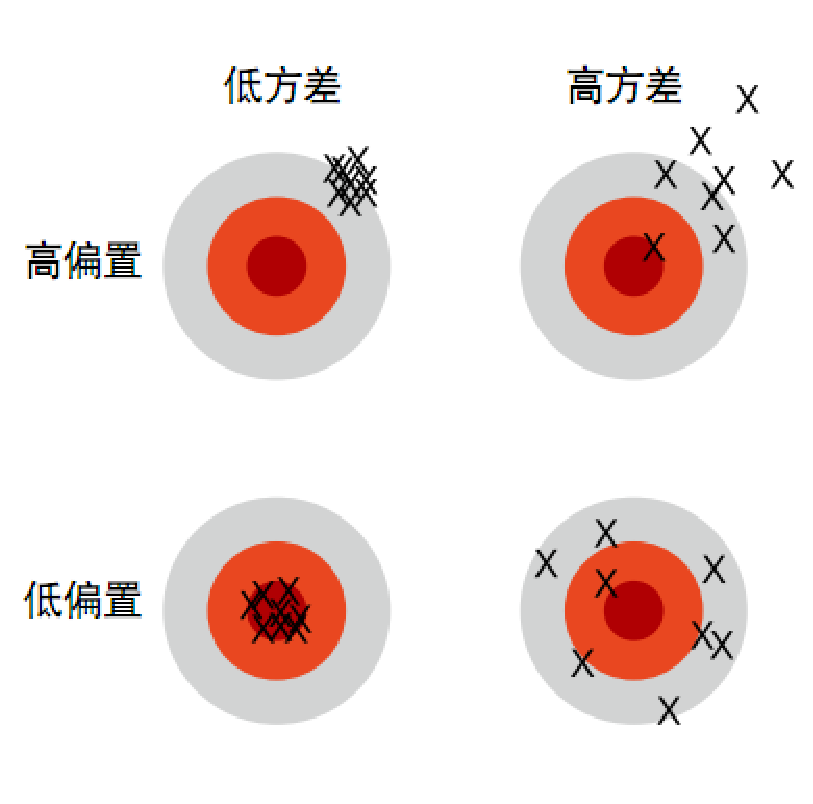
\includegraphics[width=0.45\textwidth,height=7cm]{figures/bias-variance.eps}
  \caption{飞镖投掷产生的偏置与方差}\label{fig:bias-variance}
\end{figure}

假设集成模型$F$是基本模型的凸组合:
\begin{equation}
    F= \sum\limits_i \omega_i h_i
\end{equation}
其中,$\omega_i$是基本模型$h_i$的权重,这里取$\omega_i=1/m$,$m$是基本模型的个数。

根据基本模型的平均偏差$\bar\beta_F^2$、平均方差$\bar\sigma_F^2$、平均协方差$\bar c_F$:
\begin{equation}\label{eq:averageq}
  \begin{array}{ll}
    \bar\beta_F^2 & =\frac{1}{m}\sum\limits_i (E(h_i) - y)^2 \\
    \bar\sigma_F^2 & =\frac{1}{m}\sum\limits_i E(h_i - E(h_i))^2\\
    \bar c_F & = \frac{1}{m(m-1)} \sum\limits_i \sum\limits_{j\neq i} E(h_i - E(h_i))(h_j - E(h_j))
  \end{array}
\end{equation}
分解方差项$\sigma_F^2$,从而将集成模型的预测误差分解成三个部分(Bias-Variance-Covariance分解)\cite{ueda1996generalization}:
\begin{equation}\label{eq:biasvariancecodec}
    E(F - y)^2 = E(\frac{1}{m} \sum\limits_i h_i - y)^2 = \bar\beta_F^2 + \frac{1}{m} \bar\sigma_F^2 + (1 - \frac{1}{m})\bar c_F
\end{equation}

1995年,Krogh和Vedelsby\cite{krogh1995neural}证明“集成模型的预测误差小于等于基本模型预测误差的加权平均值”(Ambiguity分解),具体地
\begin{equation}\label{eq:ambiguitydec}
    (F - y)^2 = \sum_i \omega_i(h_i - y)^2 - \sum_i \omega_i(F - h_i)^2 \le \sum_i \omega_i(h_i - y)^2
\end{equation}

Bias-Variance分解可以部分解释Boosting与Bagging集成技术的有效性,比如\cite{breiman1996bias}认为两者均能降低分类误差中的方差项,
\cite{freund1996experiments}则称Boosting能够降低分类误差中的偏差项。

\section{提升算法}
1984年,Leslie Valiant\cite{valiant1984theory}提出可能近似正确(Probably Approximately Correct,PAC)学习模型。
\footnote{Valint的PAC与Vapnik的统计学习理论(SLT),成为当今学习理论的主流,是使用最广泛的两种框架,并在实际中发展出经典的Boosting技术与SVM技术,1989 年,Anselm Blumer\cite{blumer1989learnability}等人首次将VC维与PAC联系起来。Leslie Valiant由此获得2010年的图灵奖,成为学习理论的先驱人物。}
1988年,Valiant与Kearns\cite{kearns1988learning}给出“强可学习”和“弱可学习”的概念:在PAC学习框架下,对于一个概念,如果存在一个多项式的学习算法,并且准确率很高,则称这个概念是\textbf{(强)可学习的},对应算法称为强学习算法;对于一个概念,如果存在一个多项式的学习算法,学习的准确率略高于随机猜测,则称这个概念是\textbf{弱可学习的},对应算法称为弱学习算法。与此同时,他们还提出一个开放性的问题:在PAC学习框架下,略好于随机猜测的弱学习算法能否提升为任意精度的强学习算法?如果可以,我们只要找到一种比随机猜测略好的弱学习算法就可将其提升为强学习算法,而不必费心设计出复杂的强学习算法。

1989年,Robert Schapire\cite{schapire1990strength}给出“强可学习与弱可学习等价”的数学证明,并设计出第一个多项式时间的Boosting算法;次年,Yoav Freund\cite{freund1990boosting}提出效率更高的“boost-by-majority”算法,但是两种算法都要求预先知道弱学习算法学习正确率的下限,给弱学习算法的选择设置了硬性的约束。1992年,Boosting首次用于提升神经网络模型OCR识别性能\cite{drucker1992improving,drucker1993boosting}。1995年,两人对“boost-by-majority”算法进行改进,提出了著名的AdaBoost算法(\textbf{Ada}ptive \textbf{Boost}ing)\cite{freund1995desicion}。两种算法效率相当,但AdaBoost没有对弱学习算法施加任何限制条件,更容易推广到实际应用。1999 年
\cite{schapire1999improved},两人引入置信分值的概念,将其扩展为广义的AdaBoost算法。目前,Boosting已经可以处理分类
\cite{freund1995desicion,friedman2000additive}、回归\cite{duffy2002boosting}与排序问题\cite{freund2003efficient,xu2007adarank}。

Boosting是一种典型的集成方法,其基本思想是通过迭代的方式构造弱学习器,依据弱学习器在训练集上的性能调整训练样本的权重,性能越高则权值越大,反之亦然,通过强化学习性能不佳的样例,构造出性能优良的集成模型。Boosting已经广泛应用到多个领域,如手写字符识别、图像识别及检索、文本分类、语音识别等。

对于稳定性差的学习算法,如决策树、决策树桩、神经网络,数据集的微小扰动都能明显改变学习的结果,Boosting倾向于使用它们作为弱学习算法,以增加误差产生的多样性,改善模型整体性能。
\subsection{AdaBoost}
AdaBoost算法对训练数据集每个样本赋以一个初始权值,迭代地添加弱分类器,并将选择的所有弱分类器组合作为最终的分类函数。在学习过程中,AdaBoost算法会实时调整样本权值,对当前分类函数正确分类的样本降低权值,而对错误分类的样本增加权重。
\begin{algorithm}[htbp]
        \caption{AdaBoost算法(二元分类)}
        \begin{algorithmic}
            \REQUIRE ~~训练集$S=\{x_i,y_i\}_{i=1}^n$,迭代次数$T$\\
            \STATE
            \begin{itemize}
              \item 初始化样本概率分布$P_1(i)=1/n,~~i=1,\ldots,n$
            \end{itemize}
            \FOR{$t = 1,\dots, T$}
            \STATE
            \begin{enumerate}
              \item 基于样本概率分布$P_t$训练弱学习器$h_t:X\mapsto \{-1,1\}$
              \item 计算弱学习器的分类误差
              \begin{equation}
                \epsilon_t = \sum\limits_{i=1}^n P_t(i) I(h_t(x_i)\ne y_i)
              \end{equation}
              \item 给弱学习器赋权值
                \begin{equation}
                    \alpha_t=\frac{1}{2}\log\frac{1-\epsilon_t}{\epsilon_t}
                \end{equation}
              \item 更新概率分布
              \begin{equation}
                P_{t+1}(i) = \frac{P_t(i) e^{-\alpha_t y_i h_t(x_i)}}{Z_t}
              \end{equation}
              其中,$Z_t$是标准化因子。
            \end{enumerate}
            \ENDFOR
            \ENSURE ~~最终分类模型$H(x) = \sgn\big(\sum\limits_{t=1}^T \alpha_t h_t(x)\big)$
        \end{algorithmic}
\end{algorithm}

\subsection{LPBoost}

\subsection{大间隔模型:提升算法}
1999年,Robert Freund与Yoav Schapire\cite{freund1999short}建立起Boosting同“间隔”的关系
\begin{equation}
    \rho = y f(x) = y \sum\limits_{t=1}^T \alpha_t h_t(x)\in [-1,1]
\end{equation}
其中,弱学习器$h_t$的权值$\alpha_t$为
\begin{equation}
    \alpha_t = \frac{1}{2} \log\frac{1-\sum\limits_i P_t(i) I\big[h_t(x_i)\ne y_i\big]}{\sum\limits_i P_t(i) I\big[h_t(x_i)\ne y_i\big]}.
\end{equation}

\subsection{提升算法的缺陷}
使用Boosting技术,能够在不依赖于先验知识的条件下,取得良好的预测性能。它也有缺点,比如在一定程度上依赖于训练数据集和弱学习器的选择,当训练数据小或弱学习器性能太差时,就会导致组合模型预测精度的下降。由于在迭代过程中,对噪声数据赋予了较大的权值,以增加其在后续迭代中的学习强度,从而对模型的收敛速度构成负面影响。如何选择合适的迭代次数,确定模型过拟合发生的条件,降低Boosting对噪声数据的敏感程度等,均是研究Boosting的重要课题。研究人员针对Boosting方法的缺陷陆续提出改进算法,经典的如Breiman\cite{breiman1998arcing}提出的Arching算法(Adaptive Re-sampling and Combining),Friedman等人\cite{friedman2000additive} 提出的LogitBoost 算法和Freund 的BrownBoost算法\cite{freund2001adaptive}。

\section{Bagging}
Bagging(\textbf{B}ootstrap \textbf{Agg}regat\textbf{ing})是第一个有效的集成学习算法,也是最简单的Arching(Adaptive Reweighting and Combining)方法,由Leo Breiman于1996 年发明\cite{breiman1996bagging}。 在Bagging 方法中,使用自举复制(Bootstrap Replicate)
\footnote{Bootstrap一说源自Rudolf Erich Raspe 的小说\textit{The Surprising Adventures of Baron Munchausen},主人翁Baron声称曾经揪着头发从沼泽中把自己拉出来,后来经过传播异化为拽着鞋带把自己拉起来(Pull oneself up by one's bootstraps),表示不可能完成的事。后来,计算机发明以后,机器的启动称为Boot,实际上就是Bootstrap的简写,因为计算机启动是一个很矛盾的过程:必须先运行程序,然后计算机才能启动,但是计算机不启动就无法运行程序。在统计学中,利用自举法构建新数据集的过程称为\textbf{重采样}(Resampling):从原始数据集进行多次\textbf{有放回}的采样,采样的次数等于原始数据集的大小。统计学中另外一种重采样方法是Jackknife,与Bootstrap类似,区别在它每次从样本中抽样时只是去除几个样本(而不是抽样),像小刀一样割去一部分。}
从原始数据集中产生多组新的训练集,利用这些具有差异性的数据集训练学习多个分类器,并根据多数表决方法,组合多个分类器对新样本分类。

Bagging算法的基本流程如下:
\begin{enumerate}
  \item 对原始训练集$X$,使用Boostrap方法复制构造$m$个大小与$X$相同\footnote{对于大型数据集,一般地要求每个抽样子集包含$1-1/e\approx 63.2\%$唯一样例}的训练集$S_1,S_2,\ldots,S_m$
  \item 对每个训练集$S_i$训练一个弱分类器$h_i$,$i=1,\ldots,m$
  \item 对于新的数据$x$,使用多数表决方法,综合所有弱分类器进行分类:
  \begin{equation}\label{eq:majorityvoting}
    \hat c = \argmax_{k=1,\ldots,K} n_k
  \end{equation}
  其中,$K$是分类的级别,$n_k$是预测$x$的类别为$c_k$的弱分类器个数:
  \begin{equation}
    n_k = \sum_{i=1}^m I(h_i(x) = k), k = 1,\ldots,K
  \end{equation}
\end{enumerate}

\begin{remark}
Bagging和Boosting的主要区别在于抽样方式不同,前者采用均匀抽样,而后者采用的方法在依赖于模型预测的错误率。Bagging随机选择训练集,各轮训练集之间相互独立;Boosting各轮训练集的选择与前面各轮的学习结果有关;Bagging各个预测函数没有权重,而Boosting 是有权重的;Bagging 的各个预测函数可以并行生成,而Boosting 的各个预测函数只能顺序生成。绝大多数情况,Bagging和Boosting都可以有效地提高分类的准确性,经验分析表明Boosting 略胜一筹
\cite{opitz1999popular}。
\end{remark}

\section{Stacking}
1992年,David Wolpert\cite{wolpert1992stacked}提出Stacking框架,也称“Stacking Generalization”。

\section{随机子空间法}
随机子空间法(Random Subspace Method,RSM或Attribute Bagging,AB)\cite{ho1998random,bryll2003attribute}是一种集成分类函数,属于随机森林算法的一般形式,不同的是随机森林由决策树组成,而随机子空间分类器是由任意基本分类器组成。随机子空间法已经被应用到线性分类、支持向量机、最近邻分类和其他类型的分类算法。

随机子空间法是在小样本高维度的训练数据集(小$n$大$p$)背景下提出来的,通过组合多个不同特征的分类器增加集成模型分类的互补性,对于改善模型性能大有裨益。

假设训练数据集中有$n$个样本,而每个样本的特征维数是$p$,随机子空间法的基本步骤如下:
\begin{enumerate}[(1)]
  \item 设定子空间的维度$p_0$以及弱分类器的个数$m$,一般地,$p_0 < p$。
  \item 对每个弱分类器$h_i$,从$p$个特征中不放回(Without Replacement)地选择$p_0$维特征,生成一个训练集,并训练分类器$h_i$。
  \item 对于新的样本,通过多数表决规则(Majority Voting Rule)或组合后验概率的方式,根据$m$个弱分类器的分类结果确定新样本的最终分类。
\end{enumerate}

\section{加性树丛模型}
加性树丛模型(Additive Groves,AG)~\cite{sorokina2007additive}由自举的加性模型(Bagged Additive Model)构成,以决策树为基本模型实现对非线性成分的拟合。由于它吸收了Bagging模型的思想,可通过增加迭代次数降低过拟合的风险,总体性能优于Bagging、Boosting、随机森林等决策树集成方法。
每个树丛都可以通过一组更小的树丛循环构建,从而能够在自举迭代过程,生出大小不一的一堆树丛。加性树丛模型含有两个参数:树的个数与树的大小。

\section{维数约减}
信息化技术的快速发展产生了大量高维非结构化的数据,在人脸识别、生物信息等领域,需要从高维数据中发现数据内在结构信息,并识别出本质特征。\textbf{维数约减}(Dimension Reduction),简称“\textbf{降维}”,也称\textbf{低秩近似}(Low-Rank Approximation)是处理高维数据的一种常用技术,将高维数据转至低维表达空间。

降维问题是在给定矩阵$A\in \mathbb R^{m\times n}$和数值精度$\epsilon>0$,搜索$A$的最佳近似矩阵$\hat A\in \mathbb R^{m\times n}$,即满足$\|A-\hat A\|_{\mathcal F} \le \epsilon \|A\|_{\mathcal F}$,并且在所有符合条件的矩阵集合内$\hat A$ 的\textbf{秩最小}。

\textbf{矩阵分解算法}(Matrix Factorization)是一类重要的降维工具,流行的分解算法包括LU分解(三角分解)、QR分解和奇异值分解(Singular Value Decomposition,SVD)、概率矩阵分解(Probabilistic Matrix Factorization,PMF)。\textbf{低秩模型}是高效处理高维数据的新工具,新近兴起的\textbf{稀疏表示}(Sparse Representation)和\textbf{压缩传感}(Compressed Sensing)在图像或视频压缩领域获得巨大成功,能够充分利用图像或视频的时空相关性,实现有效压缩。
\textbf{矩阵填充}(Matrix Completion)是一种特殊的低秩模型,它能够在矩阵数据部分缺失时,利用矩阵行列间的相关性恢复矩阵的低秩结构,广泛应用于机器控制、图像处理(如去噪)等领域。

\subsection{奇异值分解}
\textbf{奇异值分解}(简称SVD)是一种经典的矩阵分解方法,广泛应用于伪逆计算、信号处理,图像压缩、生物信息处理等工作。本文主要考虑实数矩阵上的分解问题。

\begin{proposition}
对于任意实数矩阵$A\in \mathbb R^{m\times n}$,矩阵$AA^T\in \mathbb R^{m\times m}$、$A^TA\in \mathbb R^{n\times n}$都是半正定矩阵,并且两者存在相同的非零特征值。假设矩阵$A^TA$的特征值是$\sigma_1^2\ge \sigma_2^2 \ge \ldots \ge \sigma_n^2\ge 0$,对应单位特征向量是$v_1, v_2,\ldots, v_n$。如果$m<n$,则$\sigma_1^2,\ldots, \sigma_m^2$也是矩阵$AA^T$的特征值,$AA^T$的对应单位特征向量是$u_1,u_2,\ldots, u_m$。如果以$u_1,u_2,\ldots,u_m$为列构成矩阵$U\in \mathbb R^{m\times m}$,以$v_1,v_2,\ldots, v_n$为列构成矩阵$V\in \mathbb R^{n\times n}$,以矩阵$A$的奇异值作为对角元的对角阵$\Sigma\in \mathbb R^{m\times n}$,则矩阵$A$可以直接表示成三个矩阵的乘积$A = U\Sigma V^T$,这种分解方法称作矩阵$A$的奇异值分解。
\end{proposition}

任意实数矩阵$A\in \mathbb R^{m\times n}$都可以分解成三个矩阵乘积的形式
\begin{equation}\label{eq:svd}
  A = U\Sigma V^T
\end{equation}
其中,$\Sigma \in \mathbb R^{m\times n}$是对角阵,$U\in \mathbb R^{m\times m}$,$V\in \mathbb R^{n\times n}$都是正交阵,即$UU^T = I_m, VV^T = I_n$。

如果将$\Sigma, U, V$分别展开,则有:
\begin{equation}
  U = (u_1,u_2,\ldots,u_m), u_i\in \mathbb R^m
\end{equation}

\begin{equation}
  V = (v_1,v_2,\ldots,v_n), v_j\in \mathbb R^n
\end{equation}

\begin{equation}
\Sigma =
\begin{bmatrix}
\sigma_1 & 0 & \cdots & 0 & 0 & \cdots & 0\\
0 & \sigma_2 & \cdots & 0 & 0 & \cdots & 0\\
0 & 0 & \ddots & 0 & 0 & \cdots & 0\\
0 & 0 & \cdots & \sigma_m & 0 & \cdots & 0
\end{bmatrix}
\end{equation}
这里假设$m<n$。

对于任意的$i\in\{1,\ldots,m\},j\in\{1,\ldots,n\}$,矩阵$U,V$ 的列向量$u_i,v_j$分别是$AA^T,A^TA$ 的特征向量,故称$u_i,v_j$ 为矩阵$A$的左、右奇异向量,$\Sigma$ 的对角元素$\sigma_i$称作矩阵$A$的奇异值,是$AA^T$或者$A^TA$特征值的算术平方根。不失一般性,假设$\sigma_1 \ge \sigma_2 \ge \ldots \ge \sigma_m$。

下文主要就这种关系给予简单证明。由于$A = U\Sigma V^T$,则$A^T = V\Sigma^T U^T$,那么
\begin{equation}
  A A^T = U\Sigma V^T V\Sigma^T U^T = U\Sigma\Sigma^T U^T =
U
\begin{bmatrix}
\sigma_1^2 & 0 & \cdots & 0\\
0 & \sigma_2^2 & \cdots & 0\\
0 & 0 & \ddots & 0\\
0 & 0 & \cdots & \sigma_m^2
\end{bmatrix}
U^T = \sum_{i=1}^m{\sigma_i^2 u_iu_i^T}
\end{equation}

类似地可得:
\begin{equation}
  A^T A = V\Sigma^T U^T U\Sigma V^T = V\Sigma^T \Sigma V^T = \sum_{j=1}^n{\sigma_j^2 v_jv_j^T}
\end{equation}

由此可得:
\begin{equation}
  A A^T u_k = \sum_{i=1}^m{\sigma_i^2 u_iu_i^T} u_k = \sigma_k^2 u_k
\end{equation}

\begin{equation}
  A^T A v_l = \sum_{j=1}^n{\sigma_j^2 v_jv_j^T} v_l = \sigma_l^2 v_l
\end{equation}
说明$u_k, v_l$分别是$AA^T,A^TA$的一个特征向量,对应的特征值分别是$\sigma_k^2,\sigma_l^2$。

SVD在实际使用时,通常仅仅选择最大的前$r$个奇异值以及$U,V$对应的$r$列向量,即可对矩阵$A$很好地近似:
\begin{equation}\label{eq:approxsvd}
    \tilde{A}_r = \sum_{i=1}^r{\sigma_i u_i v_i^T}
\end{equation}

可以证明,$\tilde{A}_r$是所有秩为$r$的$m\times n$矩阵中,与矩阵$A$最近似的矩阵。

观察$A$的分解式,可以发现:
\begin{equation}
    A = \sum_{i=1}^m{\sigma_i u_i v_i^T} = \sigma_1 u_1 v_1^T + \ldots + \sigma_m u_m v_m^T
\end{equation}
矩阵的$A$奇异值分解实际上是将其分解成一组秩为1的矩阵线性加权的形式,这里,奇异值是加权权值。从这个角度出发,我们在下文就SVD在推荐系统中的应用,介绍分解式中的矩阵$U,V$所代表的真实含义。

推荐问题通常都涉及到用户对物品的评价,从而构成系统评价矩阵$A\in \mathbb R^{m\times n}$,矩阵的行代表用户,列代表物品,通常由于用户的数目远远多于物品数量,所以有$m \gg n$。根据矩阵$U,V$的定义,它们的列向量是由$AA^T,A^TA$的(标准化的)特征向量构成。如果对评价矩阵行分块,即
\begin{equation}
  A =
    \begin{bmatrix}
        A_1\\
        A_2\\
        \vdots\\
        A_m
    \end{bmatrix}
\end{equation}
其中,$A_i\in \mathbb R^{1\times n}, 1 \le i \le m$,实际上代表一个用户评价向量。由此,可以得到
\begin{equation}
  AA^T =
    \begin{bmatrix}
        A_1\\
        A_2\\
        \vdots\\
        A_m
    \end{bmatrix}
(A_1^T, A_2^T, \ldots, A_m^T)
=
    \begin{pmatrix}
        A_1A_1^T & A_1A_2^T & \ldots & A_1A_m^T\\
        A_2A_1^T & A_2A_2^T & \ldots & A_2A_m^T\\
        \vdots & \vdots & \ddots & \vdots\\
        A_mA_1^T & A_mA_2^T & \ldots & A_mA_m^T
    \end{pmatrix}
\end{equation}

如果$A$的元素是多元评价等级,那么根据余弦相似度定义可知,$A_iA_j^T$代表用户$i,j$的评价向量内积,反映了二者之间的相似程度,如果$A$的元素是二元评价等级($0-$未评价,$1-$评价),则$A_iA_j^T$ 即是两个用户同时评价的物品数目,也是一种相似关系的度量,$AA^T$实际上就是用户群相似度矩阵。

由于矩阵$U$的列向量是由$AA^T$的标准特征向量构成,并且根据特征值与特征向量的统计学意义可知,特征值越大,对应特征向量方向上点的离散程度越高。不妨设想一下极端的情况,数据点只在两个维度(特征)上是不同的,在其他维度上数值完全一致,那么在其他维度上,点的离散程度为0,对于数据分类、聚类等任务,没有任何价值,相反,剩余两个维度是区分数据点的关键。也就是说,数据点的其他特征是冗余信息,将其删除百利而无一害。从信息熵的角度来看,混杂度越大(熵越大)的方向包含的信息量越大。

SVD的计算复杂度是$\complex(m^3 + n^3)$,在处理高维数据时会产生很大的问题。据悉,Google已经实现并行化SVD,可以扩大SVD实际应用的范围。

\begin{remark}
矩阵分解是对原始评分矩阵数据从多个维度所作的近似与还原,利用分解模型,可以构建项目间或用户间相似性矩阵(一阶或高阶),利用相似矩阵,可以进行对象的聚类分析,以簇或分组为单位可以显性地表示对象间的关系,对于理解隐语义模型内在机理大有裨益。此外,我们也可以直接从相似性矩阵的分块特征上与其他传统相似性度量进行比较和联系。我们还要思考:$AA^T$ 的特征向量同用户之间的关系?与$KNN$算法存在什么样的关联?
\end{remark}
\subsection{主成分分析}
假设多元随机变量$X = (X_1,\ldots, X_m)\in \mathbb R^{n\times m}$每个特征对应一个随机变量,每一行可以表示一个抽样数据。为了刻画特征之间的相关关系,我们可以计算所有特征序的相关系数,并构造$X$上的相关系数矩阵R。如果对原始数据逐列进行Z-Score标准化,不会影响到相关系数矩阵,则有
\[
    \bar X_1 = 0, ~~\var(X_1) = 1, ~~\text{R} = \frac{1}{n-1}X^T X.
\]
如果特征彼此间存在相关性,则会产生一定的冗余信息。为剔除冗余信息,1901年卡尔·皮尔逊Karl Pearson\cite{pearson1901liii}提出一种流行至今的线性降维方法:\textbf{主成分分析}(Principal Component Analysis,PCA)。如果多元随机变量,它利用一个特殊变换$A = (A_1, \ldots, A_m)\in \mathbb R^{m\times m}$ 重新组合原始特征集,构建出一组彼此线性无关的新特征$Y=(Y_1, \ldots, Y_m)\in \mathbb R^{n\times m}$。如果$A$满足性质
\begin{equation}
    \left\{
    \begin{array}{l}
        A_1 = \argmax\limits_{A_0}~ \var(XA_0),\\
        A_i = \argmax\limits_{A_0\perp \{A_j\}_{j=1}^{i-1}}~ \var(XA_0), 2 \le i \le m, \\
        \|A_i\|_2 = 1, 1\le i \le m.
    \end{array}
    \right.
\end{equation}
则称$A$是正交矩阵,相应地新特征
\begin{equation}
  Y_i = XA_i
\end{equation}
称作映射空间上的\textbf{第$i$个主成分},$1\le i\le m$。

\begin{proposition}
主成分相互独立,即对任意的$Y_i$与$Y_j$,都有相关系数$\rho(Y_i, Y_j) = 0$。此外,主成分和原始变量间满足相关关系$\rho(Y_i, X_j) = A_{ij}$。
\end{proposition}

\begin{proposition}
主成分方差顺次递减$\var(Y_1)\ge \var(Y_2)\ge \ldots \ge\var(Y_m)$,并且保持总方差不变,满足$\sum_{i=1}^m \var(Y_i) = \sum_{i=1}^m \var(X_i)=m$。
\end{proposition}

\begin{proposition}
假设$X$上的相关系数矩阵为R,则$A_i$是R的第$i$个特征向量,且对应特征值$\lambda_i = \var(Y_i)$,$1\le i\le m$,从而有$\lambda_1\ge \ldots \ge \lambda_m \ge 0$。
\end{proposition}

根据命题可知,主成分$Y$的方差值或相关系数矩阵R的特征值体现出原始数据的信息量,方差越大则所含信息量越大。在数据处理时,为了能够实现降维并确保最小化信息丢失,我们可以使用阈值法,比如设定一个百分比下限$\theta$,比如95\%,在前$K$个主成分的方差(相关系数矩阵R的$K$个最大特征值之和)占总方差(所有特征值之和)的比例超过$\theta$以后
\[
    \sum\limits_{i=1}^K \var(Y_i) \ge \theta \sum\limits_{i=1}^m \var(Y_i) = m \theta,
\]
则认定它们所包含的信息量足够高,从而可使用它们以近似表示原始高维空间
\begin{equation}\label{eq:pca-appr}
  \widehat Y = (Y_1,\ldots, Y_K) = X(A_1,\ldots,A_K)\in \mathbb R^{n\times K}, K \ll m.
\end{equation}

\subsection{局部线性嵌入}
局部线性嵌入(Locally linear Embedding,LLE)~\cite{belkin2001laplacian}是一种非线性降维方法,能够在降维后保持数据的原始流形结构,也是流形学习方法的一个经典工作。

\subsection{拉普拉斯特征映射}
拉普拉斯特征映射(Laplacian Eigenmaps)

\subsection{自组织映射网络}
自组织映射(Self Organizing Map,SOM)~\cite{kohonen1982self},也称自组织特征映射(Self Organizing Feature Map,SOFM)是由芬兰赫尔辛基理工大学教授Teuvo Kohonen发明的一种特殊的神经网络结构,通过无监督学习将输入样本映射至低维表示空间(二维或一维),并能保持原有数据的拓扑结构。

\subsection{自适应交叉近似算法}
自适应交叉近似算法(Adaptive Cross Approximation,ACA)是由Bebendorf和Rjasanow\cite{bebendorf2003adaptive}共同提出的一种低秩分解算法,首先将边界元(Boundary Element)矩阵分成若干块,然后对每一块(不包括对角线附近的块)做低秩分解。

传统边界元方法使用的系数矩阵$A$是满秩的,其中$A$中的每个元素都需要显式存储和参与运算。ACA算法的基本原理是:通过树状结构递归地将$A$分解为一系列子矩阵$A_{m_i\times n_i}^i$的集合,每个子矩阵对应$m_i$ 个源点和$n_i$个场点,当源点集合和场点集合距离足够远,则$A_{m_i\times n_i}^i$的秩很低,从而可以使用一组向量内积的和进行低秩近似:
\begin{equation}\label{eq:aca}
  A_{m_i\times n_i}^i \approx \sum_{l=1}^k{U_lV_l^T}
\end{equation}
其中,向量$U_l\in \mathbb R^{m_i},V_l\in \mathbb R^{n_i}$;$k$表示向量的个数,与低秩近似残差阈值$\epsilon$有关,通常$k\ll m_i$,$k\ll n_i$。由此可见,通过ACA低秩近似,对原子矩阵$A_{m_i\times n_i}^i$的存储量从$\complex(m_i n_i)$降低至$\complex[k(m_i + n_i)]$,并且在进行矩阵-向量乘积时,能够减少运算量。假设向量$X\in \mathbb R^{n_i}$
\begin{equation}
  A_{m_i\times n_i}^i X \approx (\sum_{l=1}^k{U_lV_l^T})X = \sum_{l=1}^k{w_lU_l}
\end{equation}
由此可见,矩阵-向量乘积问题就转化为简单的线性加权问题,权值为$w_l = V_l^TX,l=1,\ldots,k$,近乎线性复杂度。

\section{特征选择}
从理论上来看,特征越多则提供的信息也就越多,但是,现实世界表明,该论断并非总是成立的。特征选择(Feature Selection)有时又称特征子集选择(Feature Subset Selection,FSS)或者属性选择(Attribute Selection)
\footnote{苍梧:\href{http://www.cnblogs.com/heaad/archive/2011/01/02/1924088.html}{特征选择常用算法综述}},
属于机器学习预处理过程,通过降低数据的维数、剔除噪声数据和冗余特征,能够有效改善模型的学习精度与泛化能力,提高训练模型的效率。

%特征选择与基于映射的主成分分析,基于信息理论的维数约减技术不同,它不改变变量的原始表示。

目前,大多数特征选择的方法用于分类问题,基本上可分为三类\cite{guyon2003introduction}:过滤模式(Filter Method)\cite{mladenic1999feature}、包装模式(Wrapper Method)\cite{breiman1984classification}和嵌入模式(Embedded Method)\cite{kohavi1997wrappers}。

过滤模式将特征选择视为预处理步骤,与分类模型无关。它对每个特征计算一个相关性分值,分值低的特征将从特征空间中剔除。过滤模式易于扩展到高维特征数据,计算效率高、开销小,与具体分类模型无关。在过滤模式中,特征子集的搜索独立于模型假设空间上的搜索,并且在计算特征的相关性时,独立分析,忽视了特征之间的依存关系(Feature Dependency)。过滤模式存在两个代表性的模型:Relief 算法\cite{kira1992practical} 和Focus 算法\cite{almuallim1991learning}。

包装模式在特征子集的搜索过程,训练分类模型,使用一个预测模型给特征子集评分。包装模式对每个特征子集训练一个分类模型,模型在测试集上的预测误差用以衡量特征子集。随着特征数目的增大,特征子集的数目呈指数增加。为了搜索整个特征空间,人们陆续提出多种启发式搜索方案以搜寻最优特征子集。由于包装模式对于每个特征子集都需要训练一个预测模型,计算成本较高,并且容易产生过拟合问题。

嵌入模式在模型选择(训练、搜索)的同时选择最佳特征子集,将特征选择直接内嵌到到学习算法。与包装模式相比,嵌入模式的计算开销更小。典型的嵌入模式特征选择算法是决策树算法,如Quinlan的ID3、C4.5\cite{quinlan1986induction,quinlan1993c4}和Breiman的CART算法\cite{breiman1993classification}等,在树增长的过程,每个递归步骤都必须选择一个特征,将样本集合划分成更小的子集,选择特征的依据通常是划分以后子节点的纯度,子节点越纯则表明划分效果越佳,可见决策树生成的过程就是特征选择的过程。

\subsection{Relief}
1992年,Kira和Rendell提出了著名的Relief算法\cite{kira1992practical},它属于一种特征加权算法(Feature Weighting Algorithm),根据各个特征与类别的相关性赋予不同的权重,如果权重小于给定的阈值则将其剔除。

\subsection{贪婪搜索算法}
从整个特征空间选择特征,主要依赖两个指标:特征的重要程度、特征间的相似性。特征的重要程度容易计算,只要将单个特征独自作为一个排名模型,特征值便是预测结果,同真实相关等级比对,计算MAP、NDCG等评价指标立时可以作为特征的重要性权值。根据特征间的相似性,可以决定哪些特征可选,哪些特征冗余。但凡与已选特征高度相似的,即可认定是冗余特征,反倒是那些差异较大的特征,对于排序模型性能的提升多有裨益。计算相似性分值的指标很多,可以是余弦相似度,也可以是肯德尔距离。

假设特征空间$\mathcal F$含有$d$个特征:$\mathcal F = \{f_1, \ldots, f_d\}$,\cite{geng2007feature}通过下面的优化问题选择特征:
\begin{equation}\label{eq:mfeatureselect}
    \begin{array}{ll}
      \max\limits_a & \sum\limits_{i = 1}^d \omega_i a_i\\
      \min\limits_a & \sum\limits_{i = 1}^d \sum\limits_{j \ne i} s_{ij} a_i a_j\\
      \textit{s.t.} & a_i\in \{0, 1\}, i = 1,\ldots, d\\
      & \sum\limits_{i=1}^d a_i= m
    \end{array}
\end{equation}
其中,$a = (a_1,\ldots,a_d)$表示特征选中与否的标识,如果特征(比如$f_i$)被选中,则$a_i = 1$,否则$a_i = 0$;$\omega_i$表示特征$f_i$的权重;$s_{ij}$表示特征$f_i, f_j$的相似度,并且满足$s_{ij} = s_{ji}$;$0 < m \le d$是预先设置的入选特征的个数。

模型\eqref{eq:mfeatureselect}是个多目标优化问题,为方便计算,将其转化为单目标优化问题:
\begin{equation}\label{eq:featureselect}
    \begin{array}{ll}
      \max\limits_a & \sum\limits_{i = 1}^d \omega_i a_i - \lambda\sum\limits_{i = 1}^d \sum\limits_{j \ne i} s_{ij} a_i a_j\\
      \textit{s.t.} & a_i\in \{0, 1\}, i = 1,\ldots, d\\
      & \sum\limits_{i=1}^d a_i= m
    \end{array}
\end{equation}
模型中,参数$\lambda >0$是权衡特征重要程度与特征相似度的因子。

由于时间复杂度高达$\complex(\binom{d}{m})$,使用穷举法求解\eqref{eq:featureselect}是不现实的,自然需要构思高效的求解方法,比如Geng等人使用\textbf{贪婪搜索算法}(Greedy Search Algorithm,GSA)将时间复杂度降至$O(dm)$\cite{geng2007feature}。
\begin{algorithm}[htbp]
        \caption{GSA: Greedy Search Algorithm of Feature Selection}
        \begin{algorithmic}[1]
           \REQUIRE ~~\\
            使用特征集合$\mathcal F$中全部特征作为结点,构造无向图$G$,图中每条边的权值表示边的两个特征结点的相似度;$S$表示选中的特征集,并初始化为$S = \phi$;给定单目标优化中使用的参数$\lambda$。
            \FOR{$t = 1,\dots, m$}
            \STATE 从$G$中选取权值最大的特征结点,记为$f_{k_t}$
            \STATE 根据$f_{k_t}$与其他结点的相似度,惩罚其余诸结点,更新它们的权重:
            \[ \omega_i \leftarrow \omega_i - 2\lambda s_{ik_t}, i \ne k_t\]
            \STATE 将特征$f_{k_t}$添加至$S$中,并从$G$中剔除与结点$f_{k_t}$有关联的边:
            \[ S \leftarrow S \bigcup \{f_{k_t}\}, G \leftarrow G \setminus \{f_{k_t}\} \]
            \ENDFOR
            \ENSURE $S_m$\\
        \end{algorithmic}
\end{algorithm}

下面我们证明\cite{geng2007feature}:在不改变已入选特征的条件下,GSA能够找到\eqref{eq:featureselect}的最优解。

\begin{proof}
假设经过$t$次迭代,入选的最优特征集合$S_t = \{f_{k_i}\}_{i=1}^t$,未入选的某个结点$f_j$权值为
\begin{equation}\label{eq:weightupdate}
  \omega_j - 2\lambda \sum\limits_{i=1}^t s_{{k_i},j}
\end{equation}

根据GSA的目标函数,在第$t+1$次迭代,基于如下原则选出最佳特征:
\begin{equation}\label{eq:bestselect}
    \max~~\sum\limits_{i=1}^{t+1} \omega_{k_i} - \lambda \sum\limits_{i=1}^{t+1}\sum\limits_{j\ne i} s_{k_{t_i}k_{t_j}}
\end{equation}

由于$s_{k_{t_i}k_{t_j}} = s_{k_{t_j}k_{t_i}}$,则有$\sum\limits_{i=1}^{t+1}\sum\limits_{j\ne i} s_{k_{t_i}k_{t_j}} = 2\sum\limits_{i=1}^{t}\sum\limits_{j = i+1}^{t+1} s_{k_{t_i}k_{t_j}}$,则目标函数可分解为两部分:
\begin{equation}
  \bigg\{\sum\limits_{i=1}^t \omega_{k_i} - 2\lambda \sum\limits_{i=1}^{t-1}\sum\limits_{j = i+1}^t s_{k_{t_i}k_{t_j}}\bigg\} + \bigg\{\omega_{k_{t+1}} - 2\lambda \sum\limits_{i=1}^t s_{k_{t_i}k_{t+1}}\bigg\}
\end{equation}
第一部分是常数,因此,\eqref{eq:bestselect}等价于如下的优化问题:
\begin{equation}\label{eq:lastselect}
    \max~~\omega_j - 2\lambda \sum\limits_{i=1}^t s_{k_{t_i},j}
\end{equation}
可见,GSA搜索方法确能找到\eqref{eq:featureselect}最优解。\qedhere
\end{proof}

GAS属于过滤模式的特征选择方法,作为预处理步骤,其效果需要使用具体的排名模型予以检验。\cite{geng2007feature}使用SVMRank与RankNet两种模型试验发现,相比基准的特征选择方法信息增益(Information Gain, IG)与卡方(Chi-square,CHI),GAS表现突出。如果数据集中各个特征的表现存在明显的差异,利用特征的重要性最大化、特征间相似性最小化的原则选择特征,可以有效消除噪声的影响,效果提升相当显著。

GAS在构建无向图$G$时,需要计算所有特征对的相似度,如果数据集是高维特征,会产生大量的计算开销,制约其扩展能力。\cite{yu2009efficient} 借鉴用于分类特征提取的Relief 算法\cite{kira1992practical}提出两种特征选择模型:RankFilter与RankWrapper,扩展性能较之GAS更佳,并且计算效率较高。

\subsection{FS-BFS}
FS-BFS(Feature Selection-Best First Search)属于包装模式的特征选择方法\cite{dang2010feature},先使用Best First搜索方法把特征空间划分成$k$ 个互不相交的特征子集,再应用坐标下降法(Coordinate Descent)给特征子集赋权。FS-BFS计算开销较大,因此对于大数据集,扩展性欠缺。

\chapter{推荐系统}
传统搜索算法只能呈现给所有的用户相同的搜索结果,无法针对用户的兴趣偏好提供个性化的服务,这种在信息爆炸时信息的利用率反而降低的现象称为\textbf{信息过载}
(Information Overload)。个性化推荐,包括个性化搜索,被认为是当前解决信息过载问题最有效的工具之一。推荐是一种特殊形式的\textbf{信息过滤}
(Information Filtering),通过挖掘用户历史行为、用户间或物品间的相似关系,给网络终端用户提供符合其个性偏好的信息列表。

推荐系统是一种网络应用,可以代替用户评估其从未看过的产品,如书籍、电影、网页、酒店、音乐等,推荐经过一个从已知信息中学习,然后对未知世界进行预测的过程。一个完整的推荐系统由三个部分组成:收集用户信息的行为记录模块,分析用户偏好的模型分析模块和推荐算法模块。行为记录模块负责记录用户的偏好行为,如评价、购买、浏览、问答、下载等。模型分析模块的主要目标是使用用户行为记录模块的信息构造出用户的潜在兴趣模型。推荐算法模块则是利用后台推荐算法实时地从产品集合中筛选出用户感兴趣的产品,生成推荐列表给用户。

根据推荐算法的不同,推荐系统大致可以分成三类:\textbf{协同过滤推荐系统}、\textbf{基于内容的推荐系统}、\textbf{混合推荐系统}。

\ornamento
\section{协同过滤}
协同过滤系统是第一代被提出并得到广泛应用的推荐系统,其核心思想可以分成两部分:1)利用用户历史行为数据计算用户之间的相似性,2)根据与目标用户相似性高的用户集合(邻域)对其他物品的评价数据,预测目标用户对未知对象的偏好程度,并以此对目标用户进行推荐。协同过滤系统最大的优点是对推荐对象没有特殊的要求,它能处理音乐、电影等难以进行文本结构化表示的对象。另一方面,协同过滤系统也面临几个重要的问题:冷启动(Cold Start)、稀疏性(Sparsity)和可扩展性
(Scalability)。

协同过滤系统的算法大致可以分成两类:\textbf{基于记忆的(Memory-based)}和\textbf{基于模型(Model-based)的推荐算法}。在协同过滤系统中,建立用户与物品之间关系最常见的方式就是评分,给定一个用户,系统中物品与给定用户的关系无非是已经评价或没有评价两种。基于记忆的协同过滤系统的目标是利用系统中历史评价信息,通过用户之间或者物品之间的相似关系,预测指定用户对于未评价物品的偏好程度,从而可能给出的评分。如果系统利用的是用户之间的相似关系进行协同过滤推荐,则称此系统为\textbf{基于用户的协同过滤系统(简称UserCF)};反之,如果利用物品之间的相似关系进行预测,则称其为\textbf{基于物品的协同过滤算法(简称ItemCF)}。

我们定义如下基本的数学符号,将在本章统一使用它们:
\begin{itemize}
  \item $\mathcal U$ - 用户集合
  \item $\mathcal I$ - 物品集合
  \item $A = (r_{ui})_{m\times n}$ - 用户对物品的评分矩阵
  \item $r_{ui}$ - 用户$u$对项目$i$的历史评分
  \item $p_{ui}$ - 用户$u$对项目$i$的模型预测评分
  \item $z_{uv}$ - 如果项目集中存在至少一个项目由用户$u$和$v$ 共同评价过,则$z_{uv}=1$;否则,$z_{uv}=0$
  \item $z_{ij}$ - 如果用户集中存在至少一名用户既评价过项目$i$ 又评价过项目$j$,则$z_{ij}=1$;否则,$z_{ij}=0$
  \item $z_{ui}$ - 如果用户$u$评价过项目$i$,则$z_{ui}=1$;否则,$z_{ui}=0$
  \item $\mathcal U_i$ - 评价过物品$i\in \mathcal I$的用户集合,$\mathcal U_i=\{u\in \mathcal U|z_{ui}=1\}$
  \item $\mathcal I_u$ - 系统推荐给用户$u$或$u$评价过的商品集合,$\mathcal I_u=\{i\in \mathcal I|z_{ui}=1\}$
  \item $\mathcal U_{ij}=\mathcal U_i \bigcap \mathcal U_j=\{u\in\mathcal U|z_{ui}=z_{uj}=1\}$ - 既评价过物品$i$ 又评价过物品$j$ 的用户集合
  \item $\mathcal I_{uv}=\mathcal I_u \bigcap \mathcal I_v=\{i\in\mathcal I|z_{ui}=z_{vi}=1\}$ - 系统推荐给用户$u$和$v$相同的物品集合或两者均评价过的物品集合
  \item $\bar r_u = \frac{1}{|\mathcal I_u|} \sum\limits_{i\in\mathcal I_u} r_{ui}$ - 用户历史平均评分
  \item $\bar r_i = \frac{1}{|\mathcal U_i|} \sum\limits_{u\in\mathcal U_i} r_{ui}$ - 物品历史平均得分
  \item $s_{uv}$ - 用户$u\in \mathcal U$和$v\in \mathcal U$ 的相似度
  \item $s_{ij}$ - 物品$i\in \mathcal I$和$j\in \mathcal I$ 的相似度
  \item $\mathcal N(u;\kappa)$ - 用户集中与用户$u\in \mathcal U$相似度最高的$\kappa$名用户,也称用户$u$的$\kappa$近邻
  \item $\mathcal N(i;\kappa)$ - 物品集中与物品$i\in \mathcal I$相似度最高的$\kappa$个物品,也称物品$i$的$\kappa$近邻
\end{itemize}

在协同过滤计算时,建立用户间或项目间的相似度关系是重要的一环。目前,使用最多的相似性度量主要是余弦相似度(Cosine Similarity)、修正的余弦相似度(Adjusted Cosine Similarity)和皮尔逊相关系数(Pearson Correlation Coefficient)。给定项目$i$与$j$,两者之间的余弦相似度为评分矩阵$A$中$i$列和$j$列评分向量的余弦值:
\begin{equation}
    s_{ij} = \frac{\sum\limits_{u\in \mathcal U} r_{ui} r_{uj}}{\sqrt{\sum\limits_{u\in \mathcal U} r_{ui}^2}\sqrt{\sum\limits_{u\in \mathcal U}r_{uj}^2}}.
\end{equation}
余弦相似度度量的相似度存在一个重要的缺陷,它没有考虑到不同用户的评分尺度的差异。对于同一个项目,部分用户评分偏高,而部分用户评分又可能偏低。为了弥补这一缺陷,研究人员对余弦相似度度量进行修正,对每个评分减去对应用户的平均评分量,然后再计算项目之间的相似度:
\begin{equation}
    s_{ij} = \frac{\sum\limits_{u\in \mathcal U_{ij}} (r_{ui} - \bar r_u) (r_{uj} - \bar r_u)}{\sqrt{\sum\limits_{u\in \mathcal U_{ij}} (r_{ui}-\bar r_u)^2}\sqrt{\sum\limits_{u\in \mathcal U_{ij}}(r_{uj}-\bar r_u)^2}},
\end{equation}
其计算仅限于共同评价过两个项目的用户。

在基于物品的协同过滤推荐中,使用修正的余弦相似性度量物品间的相似性更佳,然而在基于用户的协同过滤推荐中皮尔逊相关系数更为有效~\cite{jannach2010recommender}。对于用户$u$和$v$,两者的历史平均评分分别是$\bar r_u$ 和$\bar r_v$,则有
\begin{equation}
    s_{uv} = \frac{\sum\limits_{i\in \mathcal I_{uv}} (r_{ui} - \bar r_u) (r_{vi} - \bar r_v)}{\sqrt{\sum\limits_{i\in \mathcal I_{uv}} (r_{ui}-\bar r_u)^2}\sqrt{\sum\limits_{i\in \mathcal I_{uv}}(r_{vi}-\bar r_v)^2}},
\end{equation}
其计算与修正的余弦相似度类似,仅仅限于用户$u$和$v$共同评价过的项目集$\mathcal I_{uv}$。

\subsection{基于用户的协同过滤算法}
基于用户的协同过滤算法(User-based Collaborative Filtering)根据用户之间的相似性关系,间接地预测用户$u$对物品$i$的可能评分。我们结合皮尔逊相关性度量方法,可以建立如下形式的预测模型:
\begin{equation}
    p_{ui} = \bar r_u + \frac{\sum\limits_{v \in \mathcal U_i} \gamma_{uv} (r_{vi} - \bar r_v)}{\sum\limits_{v \in \mathcal U_i} |\gamma_{uv}|},
\end{equation}
其中,$\gamma_{uv}=s_{uv}|s_{uv}|^{\rho-1}$是关于皮尔逊相关性的一种转换,以降低噪声数据对预测的干扰。实验
\cite{breese1998empirical,lemire2005slope}表明$\rho=2.5$时,可以取得不错的效果。

由皮尔逊相关性分析可知,可能存在相当比例的用户与用户$u$没有太大的相关性。为此,研究人员在相似度度量的基础上,从用户集中筛选出部分与用户$u$相关性强的用户参与运算。比如,择出最相似的部分用户$\mathcal N(u; k)$,利用它们对物品$i$的历史评分数据,基于如下公式估计用户$u$对物品$i$的评分:
\begin{equation}\label{eq:ucf}
    p_{ui} = \bar r_u + \frac{\sum\limits_{v \in \mathcal N(u; k)} s_{uv} (r_{vi} - \bar r_v)}{\sum\limits_{v \in \mathcal N(u; k)} |s_{uv}|}.
\end{equation}

\subsection{基于物品的协同过滤算法}
基于物品的协同过滤算法\cite{sarwar2001item,bell2007scalable} (Item-based Collaborative Filtering)预测用户$u$对物品$i$的评分,最基本的形式是使用用户$u$ 对物品$i$ 相似的其他物品评分的加权平均值作为预测值\cite{jannach2010recommender}
\begin{equation}\label{eq:icf}
    p_{ui} = \frac{\sum\limits_{j \in \mathcal N(i; k)} s_{ij} r_{uj}}{\sum\limits_{j \in \mathcal N(i; k)} |s_{ij}|},
\end{equation}
其中,$\mathcal N(i; k)$表示与物品$i$相似度最高的$k$个物品所构成的近邻集合。

\section{Slope One}
协同推荐算法最基本的是基于用户的协同推荐和基于物品的协同推荐算法,在处理海量数据时,由于计算量大,扩展性容易遭遇瓶颈。为此,研究人员提出许多基于模型的协同过滤算法,根据评价数据推断和学习用户的行为模型,实现高效的预测评分。2005年,Daniel Lemire 和Anna Maclachlan~\cite{lemire2005slope}提出Slope One,它是一种新颖的基于模型的评分预测模型,在处理海量数据时依然可以保证良好的运算速度与推荐效果。目前,研究人员已经将其引入到其他模型
\cite{gao2009personalized,wang2009personalized,zhang2009item,sun2011one},以改善推荐系统的推荐精度,并成为各种在线推荐系统的一个重要算法。

Slope One算法从拟合一个单变量线性回归模型出发,在不需要计算项目间或用户间相似度的基础上,确立一种评分预测的策略。假设我们使用训练集$\{x_i, y_i\}_{i=1}^n$拟合一个简单的线性回归模型$f(x)=x+b$,则根据预测误差平方和最小化,我们可以确定最佳的参数$b^*$
\begin{equation}
    b^* = \argmin\limits_{b\in \mathbb R} \frac{1}{n}\sum\limits_i \big[f(x_i) - y_i\big]^2 = \frac{1}{n}\sum\limits_i (y_i-x_i).
\end{equation}
对于新的输入数据$x_0$,我们可以利用训练得到的模型$f(x)=x+b^*$ 进行预测$y_0=f(x_0)=x_0+\sum\limits_i(y_i-x_i)/n$。如果将推荐系统所有存在共同评价用户的项目评分组成训练集$\{r_{vi},r_{vj}\}_{i,j\in \mathcal I}^{v\in \mathcal U_{ij}}$,则可以建立一种简单的线性评分预测模型。如果用户$u$只评价过项目$j$,且项目对$(i,j)$存在共同评价用户,则模型预测用户$u$对项目$i$ 的评分只依赖于他对项目$j$的历史评分、项目对$(i,j)$ 的平均评分差值
\begin{equation}
    p_{ui} = r_{uj} + \frac{1}{|\mathcal U_{ij}|} \sum\limits_{v\in \mathcal U_{ij}} (r_{vi} - r_{vj}) = r_{uj} + \delta_{ij},
\end{equation}
其中,$\delta_{ij}$为项目对$(i,j)$的平均评分差值。如果用户$u$ 评价过的项目很多,并且能够与项目$i$存在共同的评价用户,那么模型的预测就建立在所有这些历史评分的基础之上
\begin{equation}\label{eq:slopeone}
    p_{ui} = \frac{1}{|\mathcal Z_{ui}|} \sum\limits_{j\in \mathcal Z_{ui}} (r_{uj} + \delta_{ij}).
\end{equation}
集合$\mathcal Z_{ui}=\{j\in \mathcal I_u|z_{ij}=1, j\ne i\}$ 是用户$u$评价过的且与$i$享有共同评价用户的项目集合。如果评分矩阵足够稠密,则$\mathcal Z_{ui}\approx \mathcal I_u$,由此我们可以取得其近似值
\begin{equation}
    p_{ui} \approx \bar r_u + \frac{1}{|\mathcal Z_{ui}|} \sum\limits_{j\in \mathcal I_u} \delta_{ij}.
\end{equation}

\subsubsection{加权Slope One}
在实际应用中,系统中不同项目的评分数量可能存在较大差异。比如,系统中有10,000名用户曾经评价过项目对$(i,j)$,却只有区区200名用户评价过项目对$(j,k)$,显然项目对评分数量的巨大差异一定会影响到Slope One模型在预测时的偏倚。为此,Daniel Lemire 和Anna Maclachlan~\cite{lemire2005slope}利用项目对评价的数量对Slope One 进行改进,提出一种加权型的Slope One算法
\begin{equation}\label{eq:weightedslopeone}
    p_{ui} = \frac{1}{\sum\limits_{j\in \mathcal I_u\setminus \{i\}} |\mathcal U_{ij}|} \sum\limits_{j\in \mathcal I_u\setminus \{i\}} (r_{uj} + \delta_{ij})|\mathcal U_{ij}| .
\end{equation}

\subsubsection{Bi-Polar Slope One}
从数值上来看,用户对项目的评分越高表明对项目越喜欢,反之则不喜欢。然而,不同的用户对于同一个项目,可能由于个人偏好、性格的差异,相同的评分所表达的好恶强度亦有所不同。譬如,一个天性乐观的人,在评分时可能偏高,即便有些项目并非其所好,其评分可能让然会高于绝大多数评分。为了更准确地衡量其喜恶,我们可以根据其历史评分信息,对所有其打过分的项目进行划分:如果项目的得分高于用户的平均历史评分,则说明用户喜欢此项目,反之则认定其不喜欢。用户对项目的喜欢与否亦有助于我们对用户进行分组,从而建立一个更佳的预测模型。

我们假设某用户$u$喜欢的项目集为$\mathcal I_u^{+}=\{i\in\mathcal I_u|r_{ui}>\bar r_u\}$,不喜欢的项目集为$\mathcal I_u^{-}=\{i\in\mathcal I_u|r_{ui}<\bar r_u\}$。对于任意项目对$(i,j)$,我们可以划出两类特殊的用户组:两个项目都喜欢$\mathcal U_{ij}^{+}=\{u\in \mathcal U|i, j\in \mathcal I_u^{+}\}$,两个项目都不喜欢$\mathcal U_{ij}^{-}=\{u\in \mathcal U|i, j\in \mathcal I_u^{-}\}$。对于同一个项目对具有相同喜恶观念的评分对于预测评分更有价值,对应地可以计算出Slope One模型基础上的两组平均评分差值
\begin{eqnarray}
  \delta_{ij}^{+} &=& \frac{1}{|\mathcal U_{ij}^{+}|}\sum\limits_{u\in \mathcal U_{ij}^{+}} (r_{ui} - r_{uj})\\
  \delta_{ij}^{-} &=& \frac{1}{|\mathcal U_{ij}^{-}|}\sum\limits_{u\in \mathcal U_{ij}^{-}} (r_{ui} - r_{uj})
\end{eqnarray}
基于此,我们使用加权型Slope One可以建立下面形式的预测模型:
\begin{equation}\label{eq:bipolarslopeone}
    p_{ui} = \frac{1}{\sum\limits_{j\in \mathcal I_u^{+}\setminus \{i\}} |\mathcal U_{ij}^{+}|+\sum\limits_{j\in \mathcal I_u^{-}\setminus \{i\}} |\mathcal U_{ij}^{-}|} \bigg\{\sum\limits_{j\in \mathcal I_u^{+}\setminus \{i\}} (r_{uj} + \delta_{ij}^{+})|\mathcal U_{ij}^{+}| + \sum\limits_{j\in \mathcal I_u^{-}\setminus \{i\}} (r_{uj} + \delta_{ij}^{-})|\mathcal U_{ij}^{-}| \bigg\}.
\end{equation}

\section{Baseline}
协同过滤模型试图准确捕获用户对项目的评分行为,影响用户对项目评分行为的因素主要包括两部分,一部分源自于用户评分偏差,另一部分源自于项目得分偏差。利用用户评分与项目得分的系统性偏差,研究人员提出一种新的预测模型,称作基线模型\cite{koren2008factorization,koren2009bellkor,koren2011advances},其数学模型表示如下:
\begin{equation}\label{eq:baseline}
    p_{ui} = \mu + b_u + b_i
\end{equation}
其中,$\mu$表示训练集所有历史评分的平均值,$b_u$与$b_i$分别表示用户$u$评分、项目$i$得分相对$\mu$的偏差程度。一个理想的评分预测模型,预测结果与实际评分应当尽量一致,为了从训练数据集中估计出用户评分偏差、项目得分偏差,我们可以解决一个最小二乘问题:
\begin{equation}
    \min\limits_{b} \sum\limits_{u\in \mathcal U}\sum\limits_{i\in \mathcal I_u} (\mu + b_u + b_i - r_{ui})^2 + \lambda (\sum\limits_{u\in \mathcal U} b_u^2 + \sum\limits_{i\in \mathcal I} b_i^2).
\end{equation}
模型的第一项是模型预测的评分误差项,第二项属于正则化项,通过控制模型的复杂度,以期达到降低模型过拟合的作用。参数$\lambda>0$是正则化因子,其值越大则模型越不容易出现过拟合。根据梯度下降(Gradient Descent)理论,可以建立下面形式的参数更新策略:
\begin{equation}
    \left\{
        \begin{array}{lcl}
            b_u & \leftarrow & b_u - \alpha (\lambda b_u + \sum\limits_{i\in \mathcal I_u} e_{ui}),\\
            b_i & \leftarrow & b_i - \alpha (\lambda b_i + \sum\limits_{u\in \mathcal U_i} e_{ui}).
        \end{array}
    \right.
\end{equation}
其中$e_{ui}=\mu + b_u + b_i - r_{ui}$表示预测偏差,$\alpha > 0$ 表示学习率。根据梯度下降法的参数更新策略可知,用户评分偏差与项目得分偏差彼此依赖,\cite{koren2011advances}提出一种粗略的估计方案,依次计算项目得分偏差与用户评分偏差:
\begin{equation}
    \left\{
        \begin{array}{lcl}
            b_i &=& \frac{1}{\lambda_I + |\mathcal U_i|}\sum\limits_{u\in \mathcal U_i} (r_{ui} - \mu),\\
            b_u &=& \frac{1}{\lambda_U + |\mathcal I_u|}\sum\limits_{i\in \mathcal I_u} (r_{ui} - \mu - b_i).
        \end{array}
    \right.
\end{equation}

对于大型训练数据集,梯度下降法在遍历所有评分后再执行模型参数的批量更新,会产生巨大的内存开销从而影响训练速度,此时随机梯度下降法(Stochastic Gradient Descent)成为一种更佳的选择。随机梯度下降法对任意选取的每个评分项$r_{ui}$确立一个微型目标函数$\ell_{ui} = (\mu + b_u + b_i - r_{ui})^2 + \lambda (b_u^2 + b_i^2)$,以快速更新模型参数$b_u$和$b_i$:
\begin{equation}
    \left\{
        \begin{array}{lcl}
            b_u & \leftarrow & b_u - \alpha (\lambda b_u + e_{ui}),\\
            b_i & \leftarrow & b_i - \alpha (\lambda b_i + e_{ui}),
        \end{array}
    \right.
\end{equation}
它不仅计算速度快,还可以有效避免陷入局部最优。

\section{矩阵分解模型}
隐语义模型(Latent Factor Model,LFM)挖掘用户和项目的隐含特征以解释观测数据集,利用隐含特征表示用户与项目的互动行为,实现精准预测的目的。目前成熟的隐语义模型包括概率隐语义分析
(pLSA)\cite{hofmann2004latent,hofmann1999probabilistic}、隐含狄利克雷分布(Latent Dirichlet Allocation,LDA)\cite{blei2003latent}和矩阵分解模型(Matrix Factorization Model,MFM)\cite{singh2008unified}。本节主要通过SVD介绍矩阵分解模型的原理。

矩阵分解模型将用户与项目映射到一个低维度的联合隐语义空间,从而可以通过联合隐语义空间下的内积刻画用户对项目的评分行为。隐语义空间反映项目的内在特征,比如电影类型(动作片、喜剧片或纪录片等)、导演、时长等,则每一部电影都可以使用少量的内在特征来表示,用户对电影的评分则可能隐含用户对不同电影类型的差异性偏好。假设隐语义空间的维度为$k\ll m,n$,对于任意一个用户$u\in \mathcal U$,都对应一个用户隐语义向量$p_u\in \mathbb R^k$。对于任意一个项目$i\in \mathcal I$,也都对应一个项目隐语义向量$q_i\in \mathbb R^k$,则用户评分矩阵$A$就可以通过两个低秩的因子矩阵的乘积近似表示,即
\begin{equation}
    A \approx P Q^T,~~r_{ui}\approx q_i^T p_u = \sum\limits_{d=1}^k p_{ud}q_{id}.
\end{equation}
用户$u$对项目$i$特征的偏好可以使用$q_i^T p_u$进行刻画。隐语义向量参数可以通过最小化目标函数
\begin{equation}
    L(P,Q) = \sum\limits_{u\in \mathcal U}\sum\limits_{i\in I_u} (q_i^T p_u - r_{ui})^2
\end{equation}
确定。一般地,人们使用梯度下降法优化目标函数。这种是最简单的SVD 方法,为了减少模型复杂度,我们可以对目标函数添加正则化项,则有
\begin{equation}
    L(P,Q) = \sum\limits_{u\in \mathcal U}\sum\limits_{i\in I_u} (q_i^T p_u - r_{ui})^2 + \lambda (\sum\limits_{u\in \mathcal U} \|p_u\|^2 + \sum\limits_{i\in \mathcal I} \|q_i\|^2),
\end{equation}
迭代更新模型参数:
\begin{equation}
    \left\{
        \begin{array}{lcl}
            q_i & \leftarrow & q_i - \alpha (\lambda q_i + \sum\limits_{u\in \mathcal U_i} e_{ui} p_u),\\
            p_u & \leftarrow & p_u - \alpha (\lambda p_u + \sum\limits_{i\in \mathcal I_u} e_{ui} q_i).\\
        \end{array}
    \right.
\end{equation}
其中,$e_{ui}=q_i^T p_u - r_{ui}$是模型预测的偏差。这种方法称作规则化的SVD方法(Regularized Singular Value Decomposition,\textbf{RSVD})。由于用户评分习惯的差异以及项目热度的不同,可能出现存在评分偏高或偏低的情况,为降低用户评分习惯与项目热度的影响,研究人员融入基线模型,提出\textbf{有偏置的SVD预测模型}
\cite{koren2008factorization,koren2009bellkor,koren2011advances}:
\begin{equation}
    p_{ui} = \mu + b_u + b_i + q_i^T p_u,
\end{equation}
通过最小化目标函数
\begin{equation}
    L(b,p,q) = \sum\limits_{u\in \mathcal U}\sum\limits_{i\in \mathcal I_u} (\mu + b_u + b_i + q_i^T p_u - r_{ui})^2 + \lambda_1 (\sum\limits_{u\in \mathcal U} b_u^2 + \sum\limits_{i\in \mathcal I} b_i^2) + \lambda_2 (\sum\limits_{u\in \mathcal U} \|p_u\|^2 + \sum\limits_{i\in \mathcal I} \|q_i\|^2)
\end{equation}
训练模型。如果记$e_{ui}=\mu + b_u + b_i + q_i^T p_u - r_{ui}$,我们可以通过梯度下降法按照如下规则迭代更新模型参数:
\begin{equation}
    \left\{
        \begin{array}{lcl}
            b_u & \leftarrow & b_u - \alpha_1 (\lambda_1 b_u + \sum\limits_{i\in \mathcal I_u} e_{ui}),\\
            b_i & \leftarrow & b_i - \alpha_1 (\lambda_1 b_i + \sum\limits_{u\in \mathcal U_i} e_{ui}),\\
            q_i & \leftarrow & q_i - \alpha_2 (\lambda_2 q_i + \sum\limits_{u\in \mathcal U_i} e_{ui} p_u),\\
            p_u & \leftarrow & p_u - \alpha_2 (\lambda_2 p_u + \sum\limits_{i\in \mathcal I_u} e_{ui} q_i).\\
        \end{array}
    \right.
\end{equation}

用户评分数据是一种显性反馈信息,实际应用中隐性反馈(Implicit Feedback)却占据了反馈数据的绝大部分,比如用户浏览、收藏等信息皆属于用户对项目的隐性反馈数据。为了提升推荐效果,研究人员在SVD方法的基础上引入项目的隐性因子向量$z_i\in \mathbb R^k$,构建新的评分预测模型:
\begin{equation}
    p_{ui} = \mu + b_u + b_i + q_i^T (p_u + |\mathcal I_u|^{-1/2} \sum\limits_{j\in \mathcal I_u} z_j)
\end{equation}
并称其为\textbf{SVD++}。用户行为包含两部分信息:显性的评分数据$p_u$与隐性反馈数据$|\mathcal I_u|^{-1/2} \sum\limits_{j\in \mathcal I_u} z_j$,更加全面地刻画用户与项目之间的交互行为。模型参数的优化是遍历所有的评分项,按照如下策略更新参数:
\begin{equation}
    \left\{
        \begin{array}{lcl}
            b_u & \leftarrow & b_u - \alpha_1 (\lambda_1 b_u + \sum\limits_{i\in \mathcal I_u} e_{ui}),\\
            b_i & \leftarrow & b_i - \alpha_1 (\lambda_1 b_i + \sum\limits_{u\in \mathcal U_i} e_{ui}),\\
            q_i & \leftarrow & q_i - \alpha_2 \big[\lambda_2 q_i + \sum\limits_{u\in \mathcal U_i} e_{ui} (p_u + |\mathcal I_u|^{-1/2} \sum\limits_{j\in \mathcal I_u} z_j)\big],\\
            p_u & \leftarrow & p_u - \alpha_2 (\lambda_2 p_u + \sum\limits_{i\in \mathcal I_u} e_{ui} q_i),\\
            z_j & \leftarrow & z_j - \alpha_2 \big[\lambda_2 z_j + \sum\limits_{i\in \mathcal I_u} e_{ui} |\mathcal I_u|^{-1/2} q_i\big], ~~\forall j\in \mathcal I_u.
        \end{array}
    \right.
\end{equation}
对于SVD、RSVD、SVD++等模型,模型参数都可以利用随机梯度下降法进行更新,只需对原始更新策略稍作修改即可。

\section{信誉系统}
开放性的网络平台是用户交互的舞台,为了节省用户检索信息的时间,每个网站都提供了一种特殊的评价系统,利用集体的智慧,对信息进行有效的过滤,使得高质量的、有价值的信息能够以更大的概率提供给用户。比如,Netflix的电影评分系统、\href{http://www.taobao.com/}{淘宝购物网站的商品评价系统}、\href{http://www.zhihu.com/}{问答网站ZhiHu 的解答过滤显示机制}等。由于网络的开放性质,网络展示对象(图书、视频、博客、商品等)的质量、评价人评价的客观性是评价系统正常运转的保证,欺诈或作弊行为会严重损害评价系统的可信度。
为此,De Kerchove\cite{de2007iterative,de2008reputation}设计一个“信誉系统”(Reputation System),在信仰散度(Belief Divergence)的基础上提出一种迭代算法,估计评价人和受评对象的信誉。信誉系统的思想简单且易于实现,对于一个含有$m$名评价人的系统,计算复杂度为$\complex(m)$。 系统在MovieLens数据集上的实验结果表明,它可以有效对抗评价人的作弊行为。

根据信誉系统的思想,每个评价人都有一个表明其评价可信度的权重,每个受评对象也都有一个反映其品质的信誉量。假设评价系统存在$m$名评价人$\mathcal U$、$n$个受评对象$\mathcal I$,评价人$u$对受评对象$i$的评分为$0\le r_{ui}\le 1$。 我们使用符号$A$ 表示评价矩阵,$\omega_u$为评价人$u$的权重向量,$\nu_i$是受评对象$i$的信誉向量。信誉系统使用评价人的权值、评价人给出的评分综合决定受评对象的信誉量,建立如下形式的信誉公式:
\begin{equation}\label{eq:repu-item}
    \nu_i = \sum\limits_{u\in \mathcal U_i} (r_{ui} \omega_u)/\sum\limits_{u\in \mathcal U} \omega_u,~~i\in \mathcal I.
\end{equation}
反过来,信誉系统还可以根据受评对象的信誉量和评价人发出的评分,推断出评价人的权值。如果评价人的评分与受评对象的历史平均评分偏差大,则系统有理由质疑其评价的可信性,从而对其权值产生不利影响。由此构建出下面形式的权值计算模型:
\begin{equation}\label{eq:repu-rater}
    \omega_u = \lambda - \sum\limits_{i\in \mathcal I_u} (r_{ui} - \nu_i)^2, ~~u\in \mathcal U.
\end{equation}
模型中参数$\lambda>0$反映利用评分偏差区分评价人的强度。它的值越大,评分偏差对评价人的区分能力就越弱;值越小,评分偏差对评价人的区分能力就越强。当$\lambda \rightarrow \infty$时,则所有评级人的权值相等$\omega_u= \lambda$,评价产生的偏差对评价人的权重不会又任何负面影响,并且受评对象的信誉值就是其获得的所有评分均值。为了保证评价人的权重非负,一般取$\lambda>n$,并且可以证明信誉系统存在唯一的最优评级人权重向量与受评对象信誉向量。

\section{基于排序学习的推荐算法}
推荐系统的研究主要分两个方向,一类是评分预测,一类是TopN推荐。传统的基于记忆的方法(如基于用户的和基于项目的协同过滤)、基于模型的方法(如矩阵分解)都是解决评分预测问题,通过优化均方根误差(RMSE)、平均绝对误差(MAE)等指标训练模型。如果推荐系统要进行TopN 列表推荐,则它只能先预测评分,再依次对项目按照预测分值降序排列获得TopN列表。实际上,由于用户只关注项目列表,所以TopN推荐更贴近用户的需求,通过直接优化TopN列表可以更好地改善用户体验
\cite{karatzoglou2013learning}。

在信息检索中,排序学习方法以检索词-文档特征作为输入,通过学习一个排序函数对新的检索词-文档对进行相关性预测。推荐系统的主要目标是给用户提供可能感兴趣的项目列表,而用户关注的可能只是排列在前几位的项目,因此也可以归结为排序问题。推荐领域中的用户- 项目对就如同检索系统的检索词-文档对,用户对项目的评分、用户日志、项目基本属性等信息作为输入特征,可以借鉴排序学习的思想直接优化项目列表。

基于排序学习的推荐方法(Learning to Rank Based Recommendation)与基本排序学习方法类似,也分成逐点型、序对型和序列性三大类。传统的协同过滤方法(如矩阵分解)多属于逐点型方法,先预测项目评分,再根据预测结果降序排列得到一个推荐列表。这种方法仅仅考虑单个项目的评分预测精度,忽略了项目间的序列关系。本质上,评分预测就是一种回归问题。序对型方法优化项目对的偏序关系,预测一个偏序矩阵,然后再将偏序矩阵转化为一个完整的排序列表。序列型方法则直接优化整个排序列表,如优化DCG、NDCG、MAP 等,比如CofiRank\cite{weimer2007cofirank}
\footnote{\href{http://www.cofirank.org/}{CofiRank}是一种基于排名的推荐算法或称协同排名方法(Collaborative Ranking Approach),另外一个代表性的模型是MatchBox。}
就是一个典型的代表。Rank-based比Rating-based 的推荐算法应用范围更广泛,基于排序学习协同过滤方法在近几年得到了广泛的研究,比如Yue Shi等人
\cite{shi2010list} 将ListNet 同概率矩阵分解(Probabilistic Matrix Factorization, PMF)相结合,提出ListRank-MF算法。他们根据协同过滤问题的特征,巧妙的利用PMF框架,给出序列型损失函数。ListRank-MF的计算复杂度是$\complex(n)$,其中$n$ 表示训练数据集中,用户给出评价的总数,拥有强大的扩展能力,并且可以取得比CofiRank更加突出的性能。

\section{基于信用的预测}
如果把用户$u\in \mathcal U$对项目$i\in \mathcal I_u$给出的所有评分构成一个评分向量,将其所评价过的每个项目各自的平均得分$\bar r_i, i\in \mathcal I_u$构成一个相等维数的得分向量。由于每个项目可能存在多个用户对其评分,则单个项目的平均得分就反映了一种集体的评价,相对单个用户所发出的评价,其可信度更强。我们将评分向量和得分向量转换成两个相应的概率分布形式:$q_u$ 与$p_u$,利用交叉熵评价用户$u$的评分向量$q_u$相对用户$u$评价的所有项目平均得分向量$p_u$的一致性。如果将项目的平均得分视为用户对项目最可信的一种评价,则由交叉熵计算公式可得
\begin{equation}
    \textrm{CE}(p_u,q_u) = \sum\limits_{i\in \mathcal I_u} -q_{ui}\log p_{ui}, ~~u\in \mathcal U
\end{equation}
当$p_u=q_u$时,交叉熵$\textrm{CE}(p_u,q_u)=\textrm{CE}(q_u,q_u)$就是对应分布的熵,值最小而一致性最强,用户$u$作出的评价可信程度也就最高。为了直接评价两个分布的一致性,我们设计指标
\begin{equation}
    c_u = \frac{\textrm{CE}(q_u, q_u)}{\textrm{CE}(p_u, q_u)} = \frac{H(q_u)}{\textrm{CE}(p_u, q_u)},~~u\in \mathcal U.
\end{equation}
作为一致性标的准度量。

假设用户$u$对项目$i$的评价源自于两个因素,一个属于内在标准,一个是外在波动。内在标准是用户自身评分的一种稳定性的体现,模型使用用户的平均评分$\bar r_u$ 作为内在的评分标准。外在波动$\varepsilon_{ui}$是用户根据其他用户对所评项目作出评价的一种认可,可以使用所有用户对项目$i$评分的一种加权平均值作为度量外在波动的指标,即
\begin{equation}
    \left\{
    \begin{array}{rcl}
        r_{ui} &=& c_u \bar r_u + (1 - c_u) \varepsilon_{ui},\\
        \varepsilon_{ui} &=& \sum\limits_{v\in \mathcal U_i} c_v r_{vi}/\sum\limits_{v\in \mathcal U_i} c_v.
    \end{array}
    \right.
\end{equation}

\section{基于图的推荐算法}
基于图模型(Graph Model)的推荐算法研究主要包括两方面内容:图的构造与图上排名。图的构造很大程度上取决于数据,比如数据只有用户、物品及用户评价信息,我们可以据此构建最简单二分图(Bipartite Graph),根据用户对物品的评价数据建立用户与物品间的通络,构成二分图的边。如果系统数据还含有有价值的标签信息,比如用户个人信息(Profile,也称用户画像)、物品属性标签、社群标签等,我们就可以构建起三分图(Tripartite Graph)或双层图模型(Two-layer Graph Model)\cite{huang2002graph,huang2004graph},通过标签或属性数据,建立用户、物品间的充分连接。图上排名,大致可以分成三类:
(1)基于图上的随机游走\cite{haveliwala2002topic,jamali2009trustwalker},使用迭代法速求解。
(2)将推荐看做一个半监督学习问题,利用传播算法实现\cite{zhu2005semi}。
(3)基于图的Laplacian矩阵度量图中节点的相似度\cite{fouss2007random}。

\section{公开数据集:评分预测与推荐}
\subsection{MovieLens}
美国明尼苏达大学的GroupLens研究小组
\footnote{GroupLens: \href{http://www.grouplens.org/}{http://www.grouplens.org/}}
发布的MovieLens电影评分数据集
\footnote{MovieLens: \href{http://grouplens.org/datasets/movielens/}{http://grouplens.org/datasets/movielens/}}
有三种类型:MovieLens 100K、1M、10M,分别包含10,000、1,000,000、10,000,000 个用户评分。用户评分采用五分制,1 代表很不喜欢,5代表很喜欢。100K 数据集包含943名用户对1682部电影的10,000个评分数据集,其中每名用户至少评价20 部电影。每条评分数据都含有从1970 年1 月1 日起以秒计时的评分时间戳,数据稀疏度为94.96\%(评分矩阵中评分尚空的比例)。 此外,数据集还以$80:20$的比例被划分成训练集和测试集,为了进行交叉校验还可以将数据集多次进行划分,从而更客观地评价评分预测模型的性能。10M数据集还包含“标签信息”,如从IMDb获取的电影标签、用户标签。

\subsection{Netflix}
Netflix是一家在线DVD租赁网站
\footnote{Netflix: \href{http://www.netflix.com/}{http://www.netflix.com/}},
2006年10月至2009年9月期间承办了一场举世瞩目的电影评分预测竞赛。在比赛之前,Netflix的电影推荐系统CineMatch的均方根误差(RMSE)为0.9525。根据比赛规定,参赛者只要可以将系统预测精度提升10\%,就可以获得Netflix提供的100万美元奖金。最终,Korbell团队通过融合107种算法赢得这份奖金。分析Korbell团队的源代码发现,奇异值分解(Singular Value Decomposition,SVD)和限制型玻尔兹曼机(Restricted Boltzmann Machine,RBM)是两种最有效的算法,二者预测结果的RMSE分别为0.8914和0.8990,如果将二者线性融合就可以将RMSE降低至0.88。竞赛所使用的数据集包含Netflix网站480,189名用户对17,770部影片的评分记录。

\subsection{百度电影推荐算法创新大赛}
百度公司在2013年3月1日组织了一项历时两月的电影推荐算法创新大赛
\footnote{\href{http://openresearch.baidu.com/}{电影推荐算法创新大赛}},
向参赛者提供了大约10,000名用户的8,000 部电影评分数据,评分采用五分制。数据集含有五个文件:
\begin{enumerate}
    \item 训练集是用户评分数据,分成用户ID、电影ID和用户对电影评分三列。
    \item 预测集只有用户ID、电影ID两列,用户对电影的评分数据是参赛者提交的结果。
    \item 电影标签含有电影ID及逗号间隔的标签列表。
    \item 用户的社交数据包括用户ID,关注此用户的用户ID(Follows)。
    \item 用户的历史观影列表,一列为用户ID,一列为电影ID。
\end{enumerate}
评价预测精度的指标是均方根误差。

\chapter{信息抽取}
\section{VIPS}
通常,网页解析皆基于“一个页面只存在一个主题”的假设进行。事实上,多个主题同时出现在同一个页面上的情形并不鲜见,尤其是列表类型的网页,既然如此,理应将页面分割成独立的语义块,分而治之。Cai等人根据人们浏览网页信息时的视觉行为,提出一种经典的页面分割模型:VIPS\cite{cai2003vips},用以抽取网页的语义结构。

\section{手写字识别}%Handwriting Recognition

\section{OCR}
光学字符识别(Optical Character Recognition,OCR)是一种将手写或机打文字的扫描图像转换成机器编码文本的机制,有时也用来称呼执行此类转换的软件。OCR 是数字化发展需求的产物,以期将机打文字转换为可以检索的数字化文本,在机器翻译,文本挖掘中应用较多。OCR涉及到多个领域的知识,如模式识别、人工智能和计算机视觉。

\chapter{机器学习基础知识}
\section{泛化能力}
泛化能力(Generalization Ability)是机器学习中的一个重要概念。机器学习方法从训练集中训练得到的模型,其泛化能力是通过模型在未知数据(测试集)上的表现反映:模型在测试集上的表现越好,表明模型的泛化能力越强,反之,则越弱。泛化能力差的模型,存在两种状态:欠拟合(Underfitting)与过拟合(Overfitting)。欠拟合模型在训练集与测试集上的表现都比较差,产生高偏置。过拟合在训练集上的表现好,但是在测试集上的表现则差强人意,对应着高方差。在学习系统中,影响模型泛化能力的因素很多,如训练集中包含的样本数目、模型的复杂度等\cite{freund2003efficient}。

在机器学习理论分析时,存在几种常见的保证泛化能力的分析方法,如保证泛化所需样本数目的边界、渐进分析(Asymptotic Analysis)等。如果一个分类器的真实错误了大于$\epsilon$,则称分类器是坏分类器。一个坏分类器在$n$个随机独立训练样本上均保持正确的概率小于$(1-\epsilon)^n$。如果假设空间$H$中有$b$个坏分类器,则至少有一个能够在$n$个随机独立训练样本上保持正确的概率小于$b(1-\epsilon)^n$,即“\textbf{一致限(Union Bound)}”。假设学习到的分类器模型在训练集上保持正确,由于$b\le |H|$,则它是坏分类器的概率小于$|H|(1-\epsilon)^n$。此概率小于$\delta>0$的充要条件是$n>\ln(\delta/H)/(1-\epsilon)$。

\section{交叉验证}
交叉验证方法(Cross Validation,简称CV)。CV是用来验证模型性能的一种统计分析方法,其基本思想是将原始数据集分组,一部分用作训练集(Training Set),另一部分作为验证集(Validation Set),使用训练集训练模型,在验证集上测试训练的模型,以此作为评价模型性能的标准。常见的CV 方法有三种:

\subsection{Hold-Out方法}
将原始数据随机分成两组,一组作为训练集,一组作为验证集,使用训练集训练模型,在验证集上测试训练的模型,并记录模型精度作为衡量模型性能的标准。这种方法简洁易于实现,只要将原始数据集随机分为两组即可,严格来说算不上CV,因为它没有反映交叉的思想,模型在验证集上的精度与原始数据集的分值有很大的关联,训练得到的模型说服力很弱。

\subsection{K折交叉验证}
K折交叉验证方法(K-fold Cross Validation,K-CV),将原始数据平均分成$K$组,轮流选择一个子集作为验证集,其他$K-1$个子集作为训练集,从而训练得到$K$ 个模型,如图~\ref{fig:4-cv}。使用$K$个模型在相应验证集上的预测精度均值表示模型性能。$K$值一般不小于2,常见的是$K=5,10$,并且只有在原始数据量很小时,才会尝试取$K=2$,有效避免过学习或欠学习的发生,最终训练得到的模型也比较具有说服力量。
\begin{figure}[htbp]
  \centering
  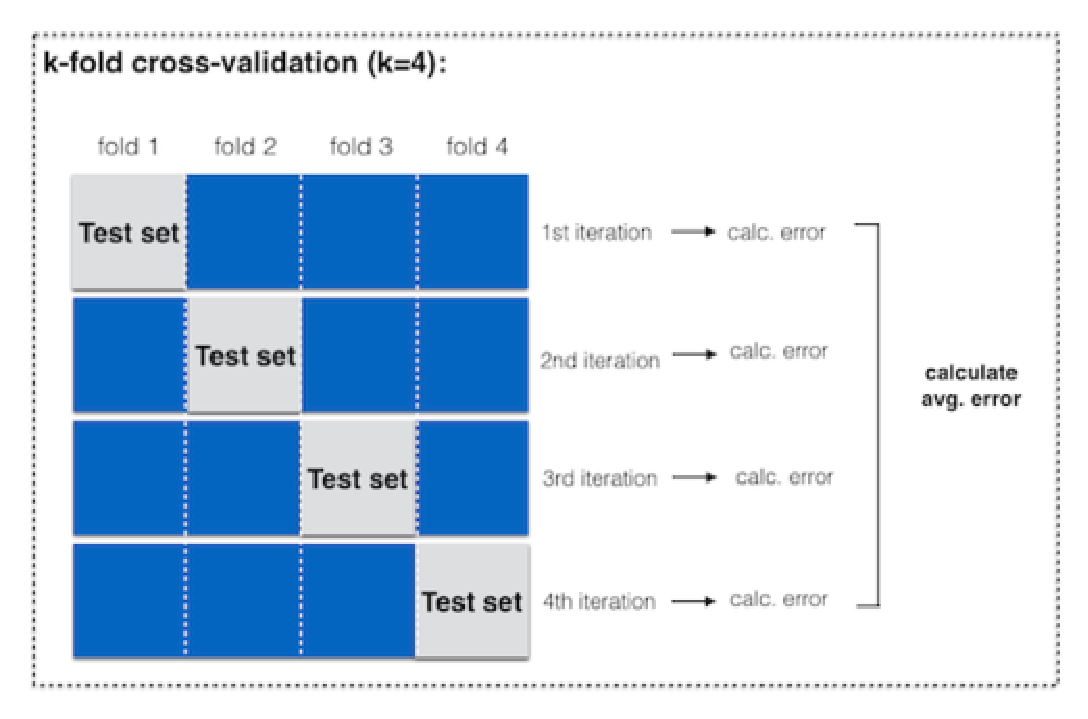
\includegraphics[width=0.6\textwidth,height=7cm]{figures/4-cv.eps}\\
  \caption{四折交叉验证}\label{fig:4-cv}
\end{figure}

\subsection{留一交叉验证}
留一交叉验证方法(Leave-One-Out Cross Validation,记为LOO-CV)是K折交叉验证方法$K=N$时的一个特例,轮换使用一个样本作为验证数据,其他$N-1$个样本构成训练集,训练得到$N$个模型,并根据它们在相应验证样本上预测精度的均值衡量模型性能。LOO-CV 的缺点是计算成本高,但相比K-CV方法,存在两个优点:
\begin{itemize}
  \item 每一回合,几乎全部样本皆用于训练模型,与原始样本的分布比较接近,训练与评估结果都比较可信。
  \item 实验过程没有引入随机因素,实验过程完全可以重现,进行不同模型的比较分析。
\end{itemize}

\section{奥卡姆剃刀}
奥卡姆剃刀(Occam's Razor)原理是由14世纪逻辑学家、修士William of Occam提出的一种逻辑或者解决问题需要遵循的基本原则,可以归纳为一句话:在假设空间中,最简单的那个假设(朴素原则)应当优先考虑。比如,将奥卡姆剃刀原理应用到模型选择问题时,应当遵循的基本原则是“在所有可能选择的模型中,能够很好地解释已知数据且形式简单的模型才是最好的模型,应该优先考虑”\cite{li2012statlearning}。

\section{没有免费午餐定理}%No Free Lunch

\section{经验法则}%Rules of Thumb

\section{贪婪算法}%Greedy Algorithm

\section{在线机器学习}
在线机器学习(Online Machine Learning)算法属于一种归纳模型,每次迭代只学习一个样例。在线学习算法主要用于样本预测,如给定一组可以描述今天股票市场的样本,在线学习算法能够预测某支股票明天的价格。在线学习的典型特征是预测的即时性,一旦发现新的样本标记,便可使用它修正在线学习算法的模型假设,从而不断地改善预测模型的表现。感知器算法、Pegasos算法与Winnow算法是三个经典的在线学习算法。

一般地,在线学习算法是通过持续的试错学习实现逐步演化,每次试错学习都包含三个步骤:
\begin{itemize}
  \item 接收一个新的样例$x$
  \item 预测样例的标记$\tilde{y} = f(\omega,x)$
  \item 接收样例的真实标记$y$,更新模型$\omega$
\end{itemize}
第三步是最关键的一步,学习算法充分利用样例的真实标记调整、更新假设模型。在模型调整时,在线学习算法通常依赖于标准的性能指标,如均方差、错误分类的比例最小化等。只要保证新样本的不断出现,在线学习算法可以持续地学习与改善,稳定性高、可扩展性强。

\section{超参数优选}%Hyper-parameter Learning
标准的监督学习包括两个重要环节:在训练集与验证集上训练和选择模型,在测试集上测试模型。模型训练阶段,一般都涉及到参数优选过程。对于某些模型,存在一类称作\textbf{超参数}(Hyper-parameter)的特殊参数,在训练之前就需要指定,如KNN模型中的$K$,神经网络模型中的隐藏层层数和隐藏层节点个数等。超参数对于模型性能影响较大,常用的\textbf{超参数优选方法}是\textbf{交叉验证方法},下文以线性回归分析为例,介绍使用K折交叉验证方法优选超参数的基本流程。

线性回归分析的目标是最小化模型$f(x,\theta) = \theta^T x$在训练数据集$S_\textrm{Train}$上的经验风险损失
\begin{equation}
    L(S_\textrm{Train}, \theta, \lambda) = \frac{1}{2n_\textrm{train}} \sum\limits_{(x,y)\in S_\textrm{Train}} \big[y - f(x, \theta)\big]^2 + \lambda \theta^T \theta
\end{equation}
第一部分表示均方差项,第二部分表示正则化项,$\lambda>0$是正则化因子,属于超参数,限定选择范围$\{\lambda_1,\ldots,\lambda_m\}$。

\begin{enumerate}[Step 1. ]
  \item 将原始数据集按照一定比例分成$A$和$B$两部分,数据$B$ 作为测试集不参与模型训练与选择,在数据$A$上使用K折交叉验证选择合适的超参数。表
  \ref{tbl:fivefoldcv}是5折交叉验证数据:数据$A$等分成五份$S_1, S_2, S_3, S_4, S_5$,轮换使用一个子集作为验证集,其它子集作为训练集,产生五折交叉验证数据集
    \begin{table}[htbp]
    \caption{五折交叉验证数据集}
    \label{tbl:fivefoldcv}
    \centering
    \begin{tabular}{c|c|c}
      \hline
      Fold & 训练集 & 验证集\\
      \hline
      Fold1 & $S_2,S_3,S_4,S_5$ & $S_1$ \\
      Fold2 & $S_1,S_3,S_4,S_5$ & $S_2$ \\
      Fold3 & $S_1,S_2,S_4,S_5$ & $S_3$ \\
      Fold4 & $S_1,S_2,S_3,S_5$ & $S_4$ \\
      Fold5 & $S_1,S_2,S_3,S_4$ & $S_5$ \\
      \hline
    \end{tabular}
    \end{table}
  \item 选择超参数$\lambda_1$,通过最小化Fold1训练集$S_\textrm{Train}=\{S_2,S_3,S_4,S_5\}$上的经验风险损失函数训练模型
      \begin{equation}
        \theta_\textrm{Train}^1 = \argmin\limits_{\theta}~~L(S_\textrm{Train}, \theta, \lambda_1)
      \end{equation}
  \item 在Fold1中验证集$S_1$上计算模型的经验风险损失
   \begin{equation}
      L_{11} = L(S_\textrm{Vali}, \theta_\textrm{Train}^1, \lambda_1)
   \end{equation}
  \item 在其他折执行上两步,在对应折训练集上训练模型,并在对应验证集上评估模型的经验风险损失$L_{12},\ldots,L_{15}$,计算平均损失$L_1=\sum\limits_{i=1}^5 L_{1i}/5$。
  \item 对于每个超参数$\lambda_i$执行上述步骤,计算平均性能$L_i$,选择平均损失最小的超参数$\lambda^*$作为最佳超参数,并使用它在数据集$A$上训练模型,得到最优参数$\theta^*,\lambda^*$。
  \item 根据训练的模型,在测试集$B$上测试模型,计算模型的预测损失
  \begin{equation}
    \frac{1}{2n_\textrm{test}} \sum\limits_{(x,y)\in S_\textrm{Test}} \big[y - f(x, \theta^*)\big]^2
  \end{equation}
\end{enumerate}

使用交叉验证的方法优选超参数计算开销大,目前存在几种流行的近似优化方法,如网格搜索、随机搜索\cite{bergstra2012random}。根据\cite{bergstra2012random}实验结果,对于含有多个超参数的模型,随机搜索远比网格搜索效率高而且效果更佳。Metzler和Croft\cite{metzler2007linear}使用一种监督学习的方法进行参数优化。他们认为直接优化线性模型标准度量方式(如MAP,P@10),可以通过网格搜索或坐标上升算法予以解决。由于标准度量模型是非平滑,直接优化标准度量,传统的优化算法无能为力。他们认为,在高维空间,搜索标准度量的最大值点十分困难,但是如果能够选取合适的细粒度(Granularity),网格搜索算法就可以找到全局最大值点;坐标上升算法属于局部搜索方法,在标准度量为凹函数时,无法保证找到全局最大值点。如果标准度量包含多个局部最值点,可以通过重启动(restart)提高找到全局最优点的几率。Metzler 和Croft 在文中使用的就是坐标上升算法,每次搜索伴以10次随机重启(10 Random Restarts)。

\section{P/NP问题}
计算复杂度理论(Computational Complexity Theory)主要研究对象是计算机求解问题的速度,比如解决问题所需时间、内存空间、处理器等资源。复杂度理论将所有可以在\textbf{多项式时间}(Polynomial Time)内解决的问题划分为\textbf{P问题}。对于一个问题$S$,如果存在算法$A$,可以在$n^k$时间内解决问题$S$或者说它的时间复杂度是$O(n^k)$,其中$n$是输入大小,$k$是一个自然数,则$S$存在一个多项式时间算法。我们提供给算法$A$一个问题的可能答案,如果算法可以在多项式时间内验证此解正确与否,那么算法$A$ 就是一个\textbf{不确定性算法}(Nondeterministic Algorithm)。所有使用不确定算法在多项式时间内可以解决的问题统称\textbf{NP 问题},它可以在多项式时间内得到验证。由此可知,P 问题是NP问题的一个子集,即P$\subseteq$NP。如果一个NP问题的所有可能答案,都可以在多项式时间内进行正确与否的验证,则称它为\textbf{NP完全问题}(NP-Complete Problem, NPC)。

\begin{example}[子集加和问题]
给定一个整数集合,它的一个非空子集的所有元素加和是否等于零?比如集合$\{-2, -3, 15, 14, 7, -10\}$,我们可以迅速地给出肯定的答复,但是不存在一个多项式时间复杂度的算法构造一个加和为零的子集。子集加和问题是一个典型的NP问题,但不一定是P问题。
\end{example}

2000年,美国Clay数学研究所(Clay Mathematics Institute, CMI)收录七个千禧年数学难题,每个奖金一百万美元,排在第一问的是\textbf{P 对NP 问题}(P v.s. NP Problem)
\[P\stackrel{?}{=} \mathrm{NP}.\]
它是由著名计算机科学家、1982年度图灵奖得主Stephen A. Cook\cite{cook1971complexity}在1971年发现并提出的一个难题。它的意思是:对于任意一个问题,如果它的解可以使用计算机\textbf{迅速}(多项式时间)验证,这个问题是否同样可以使用计算机\textbf{迅速}求解。
Cook举了一个有趣的例子形象地解释它:在一个周六的晚上,你参加了一个盛大的晚会,感到局促不安,你想知道大厅里是否有你认识的人。晚会的主人道:“你一定认识那位正在甜点盘附近的女士罗丝”。你只需向主人所指的方向扫一眼,也许发现他/她是正确的。如果缺少这样的暗示,你需要环顾整个大厅,一个个地审视。生成问题的一个解通常比验证给定的一个解所花费的时间多得多。

\section{收敛速度与复杂度}
假设数值迭代算法生成的序列为$\{x_k\}$,若序列收敛并且等式
\begin{equation}
    \hat x = \lim\limits_{k\rightarrow \infty} x_k
\end{equation}
成立。如果存在$\mu\ge 0$,使得
\begin{equation}
    \mu = \lim\limits_{k\rightarrow \infty} \frac{\|x_{k+1} - \hat x\|}{\|x_k - \hat x\|}
\end{equation}
则$\mu$称为序列$\{x_k\}$的\textbf{收敛速率}(Convergence Rate)。如果$\mu\in(0,1)$,则称序列\textbf{线性收敛};如果$\mu=0$,则称序列\textbf{超线性收敛};如果$\mu=1$,则称序列\textbf{次线性收敛}。
如果序列次线性收敛,并且满足下式:
\begin{equation}
    \lim\limits_{k\rightarrow \infty} \frac{\|x_{k+2} - x_{k+1}\|}{\|x_{k+1}-x_k \|} = 1
\end{equation}
则称序列\textbf{对数收敛}至$\hat x$。

为了对超线性收敛细分,定义$q$-阶收敛速率
\begin{equation}
    \mu = \lim\limits_{k\rightarrow \infty} \frac{\|x_{k+1} - \hat x\|}{\|x_k - \hat x\|^q} >0
\end{equation}
其中,阶数$q>1$。当$q=2$时,则称序列\textbf{二阶收敛}。

在表示算法时空复杂度时,通常在渐进表示法(Asymptotic Notation)中使用$\mathcal O$表示渐进上界(最坏表现),$\Omega$ 表示渐进下界(最佳表现),$\Theta$ 表示是一种相对比较精确的方法。在实际应用中,以$\mathcal O$使用最为常见。

\section{适定问题与非适定问题}
1902年,法国数学家Jacques Hadamard\cite{hadamard1902problemes}在研究偏微分方程时提出适定问题(well-posed problem),认为所有刻画物理现象的数学模型都应该是适定的,即数学模型的解满足:存在性、唯一性和稳定性(模型解对初值变化连续)。在实际问题中,Hadamard意义下的适定条件并不通用,它无法解释部分模型对于数据微小扰动的敏感性,引发解的剧烈变化。如果数学模型只满足部分条件,就称作不适定问题(ill-posed problem),或模型不适定。比如,图像处理中遇到的不适定问题有:去噪(De-nosing)、复原(Restorsion)、放大(Zooming)、修补(Inpainting)、去马赛克(Demosaicing)、超分辨(Super-resolution)等。

解决不适定问题的方法有很多,其中一个最常使用的方法是Tikhonov 正则化,通过限定假设空间将原问题转化为适定问题。在统计学中,Tikhonov正则化方法应用于线性回归分析,称为岭回归。

\section{欠定系统与超定系统}
当线性方程组中未知数的数目大于方程的数目,则称线性系统\textbf{欠定}(Under Determined),反之则称线性系统\textbf{超定}(Over Determined)。如果线性方程系统没有解,则称它是具有\textbf{非一致性}(Inconsistent)线性方程系统。根据Rouch\'{e}–Capelli定理,当线性方程组增广矩阵的秩与系数矩阵的秩相对,则线性方程组存在唯一解;当增广矩阵的秩大于系数矩阵的秩时,则线性方程组无界;否则,它有无穷多解。欠定系统要么存在无穷多解,要么没有解。
%-------------data mining & machine learning
\chapter{排序学习}\label{chapt:l2r}

互联网的蓬勃发展,尤其是社交网络的诞生,一改往日“信息匮乏”的局面,大数据时代已经来临。搜索引擎是网络用户从海量数据中查找信息的主要入口,因此,如何根据用户的检索请求,迅速地准确定位到相关信息源(如网页、文档、音频、视频、图片等),是搜索引擎能否为用户认可,能否吸引用户的重要标准,而搜索核心环节就是排序:将搜索内容以列表的形式,按照相关程度从高到低展现给用户。

传统的搜索排序主要基于手工构造的模型,计算文档与检索词之间的相关程度。传统的排序模型大致可分为两种类型,基于链接分析的模型,如PageRank\cite{brin1998anatomy,page1999pagerank}, HITS\cite{kleinberg1999authoritative},SALSA\cite{lempel2000stochastic,lempel2001salsa};基于内容分析的模型,如向量空间模型\cite{salton1975vector},BM25\cite{robertson2009probabilistic}。目前影响网页排名的因素有上千种,传统排名算法面对这种复杂局面,存在以下几个方面的不足:(1)考虑的影响因素比较单一;(2)对多个影响因素的融合能力较差;(3)使用时不够灵活;(5)对复杂模型的参数调整比较困难。
\begin{figure}[htbp]
  \centering
  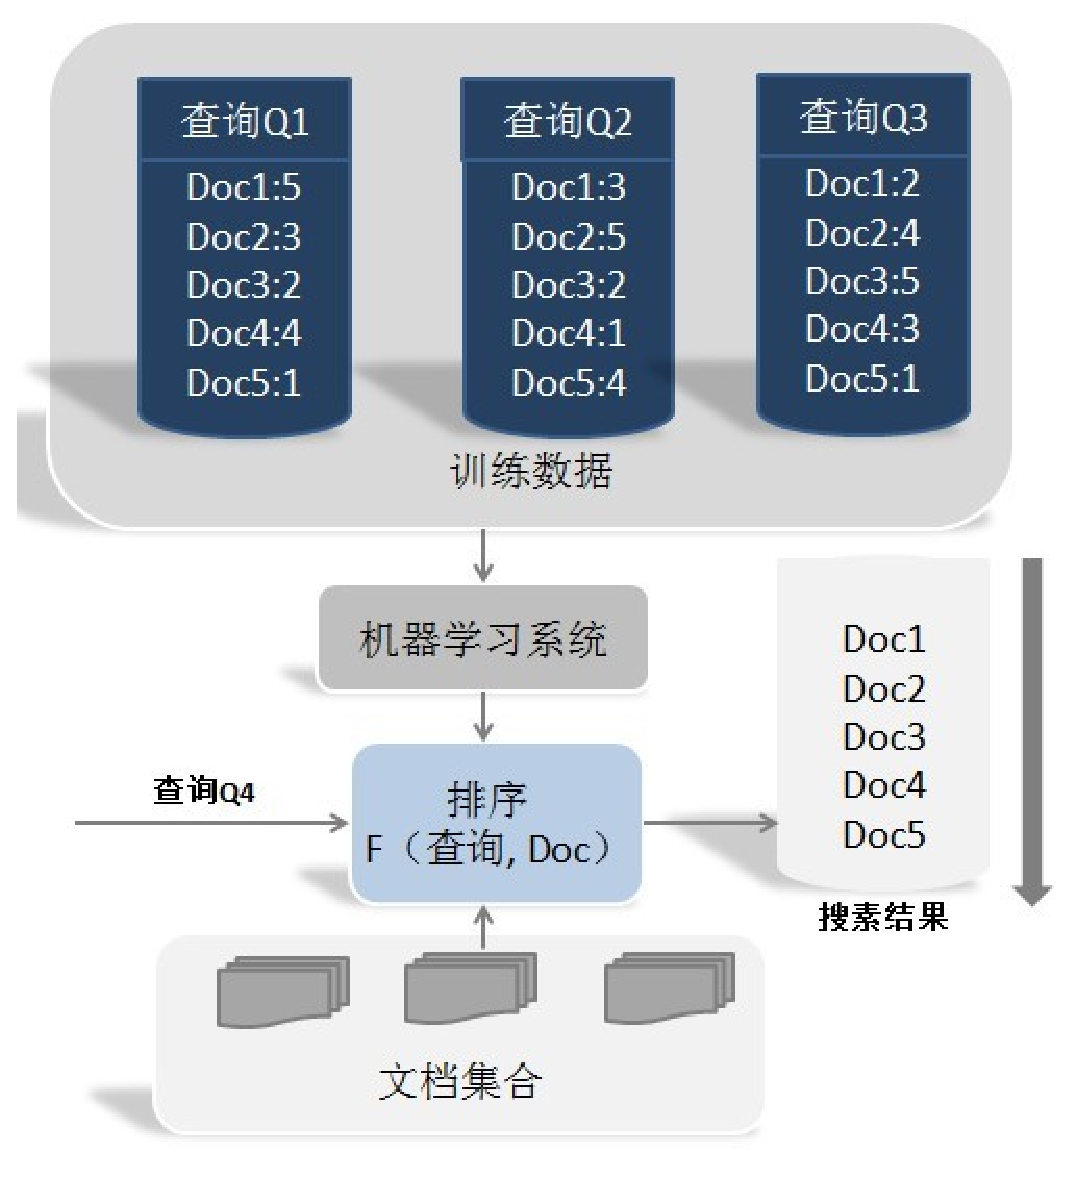
\includegraphics[width=0.5\textwidth,height=8cm]{figures/l2r.eps}
  \caption{排序学习框架}\label{fig:l2rframwork}
\end{figure}

排序学习\cite{trotman2005learning,liu2009learning}可以在一定程度上克服传统排序的缺点。它结合机器学习的方法,可以自动地从训练数据集中学习排名函数。序列型排序学习方法是目前最直接,也是表现最好的一类排序学习方法。排序学习是一种典型的监督学习方法,需要利用带有人工标记的标准数据集训练模型。数据集一般包含多个检索词,每个检索词存在多个关联文档,每个文档由一个多维特征向量(每个特征都可以单独作为一个排名函数,如PageRank,TF*IDF等)表示,相应地,每篇文档都有一个人工标记的相关等级,反映文档同检索词的相关程度。

\ornamento
\section{背景介绍}
排序学习方法是一种有效的排名技术,借鉴机器学习的监督学习方法,通过优化损失函数,从训练数据集中学习一个排名函数。排序学习是一个较新的研究方向,在过去十年间发展迅速,已经被成功地应用到网页搜索、机器翻译和系统推荐等领域\cite{liu2009learning}。

Liu\cite{liu2011learning}和Li\cite{li2011learning}根据输入空间、输出空间、模型假设和损失函数的不同,将排序学习方法划分为三类:逐点型(Pointwise)、序对型(Pairwise)、序列型(Listwise)。

逐点型排序学习方法将排名问题转化为传统的分类、(有序)回归问题,根据成熟的分类和回归算法,使用分类错误率或者均方差构建损失函数,训练排名函数。比如,Crammer和Singer\cite{crammer2001pranking}提出的PRank算法,通过训练一个感知器模型,把训练样本映射到一个全序集。

序对型排序学习算法的训练数据是成对的样本,根据模型假设预测序对的偏好关系,结合真实相关等级,构造序对损失函数,模型训练的目标即最小化序对损失函数。典型的序对型排序学习算法有:Herbrich等人\cite{herbrich1999large}将排序问题转化为序对型分类问题,基于支持向量机(Support Vector Machine, SVM)提出RankingSVM 算法;Freund等人\cite{freund2003efficient}根据提升(Boosting)技术,将用于分类的经典算法AdaBoost应用到序对型排序学习问题,提出了RankBoost算法;Burges等人\cite{burges2005learning}根据神经网络(Artificial Neural Network, ANN)的进化学习理论,辅以梯度下降的优化方法调整模型参数,训练排序模型,提出RankNet 算法;由于标准评价指标是非平滑不可微的,无法直接优化,Burges等人\cite{burges2007learning}分析交换序对文档名次引发的成本变化,直接定义损失函数的梯度
(Lambda),改进RankNet算法引入LambdaRank。

序列型排序学习方法直接将整个样本集合作为学习对象,根据模型的预测结果和真实排名列表构建出序列型损失函数,通过优化序列型损失函数训练排序模型。比如,2007 年Xu和Li\cite{xu2007adarank}基于Boosting技术,以单个特征作为备选弱排名函数,提出一种高效的学习算法——AdaRank。同年,Cao等人\cite{cao2007learning}认为在训练过程中,RankNet算法使用的交叉熵损失函数降低的同时却无法保证标准度量指标相应地提升,于是提出一种基于概率模型的排序模型ListNet。ListNet是RankNet的一种序列型扩展。Qin等人\cite{qin2008query}提出的RankCosine算法是基于余弦损失函数,使用梯度下降法在神经网络上训练模型。Xia等人\cite{xia2008listwise}于2008年提出的ListMLE算法同ListNet类似,都是基于Plackett-Luce概率模型、神经网络技术和梯度下降法训练排名函数,但是ListMLE根据真实排名列表,假设列表中各个位置服从指数概率分布,并根据最大似然估计,定义似然损失函数。

由于衡量排序性能的标准评价指标需要考虑文档位置信息,因此是非平滑的不可微函数,序列型排序学习方法“直接”优化目标多是对性能指标作平滑近似或者通过寻找性能评价指标的平滑上界,间接地进行优化。如Taylor等人\cite{taylor2008softrank}提出的SoftRank算法根据模型的预测结果,使用SoftNDCG近似文档的排名分布,属于平滑近似方法。Yue等人\cite{yue2007support}提出的SVM\textsuperscript{MAP}模型和Chakrabarti等人\cite{chakrabarti2008structured}推出的SVM\textsuperscript{NDCG}模型分别对标准评价指标MAP和NDCG估计出其平滑上界,均属于确定平滑上界的方法。

序列型排序学习方法实际上是直接优化性能评价指标,相比逐点型、序对型排序学习方法而言,训练过程较为直观,损失函数同性能评价指标之间的一致性更强,而且不易受检索词关联文档数目差异的影响。序列型排序学习方法内在地要优于序对型排序学习方法。

\section{研究团队}
目前研究排序学习的主要团队有微软亚洲研究院(如Hang Li,Tie-Yan Liu等),微软Bing搜索已经使用RankNet算法,但更偏重于理论证明。
俄罗斯的Yandex研究团队在2009年Yahoo!举办的Learning to Rank Challenge中取得不错的名次,而且据说Yandex 搜索引擎已经开始使用排序学习训练的模型改善搜索质量。据称,Yandex 从2009年开始使用一种新的机器学习模型MatrixNet,融合了上千种搜索因素,极大地改善搜索的质量。Yandex还举办了Internet Mathematics 2009竞赛。2002年前后,AltaVista首先使用Boosted Tree Regression构建基于排序学习的排名系统,系统上线后,排名第一的网页点击率有明显提升。百度网页搜索于2011年左右引入机器排序学习,并发布排序学习算法工程师的招聘通知。Google对排序学习的兴趣不高;Cuil的CEO认为由机器学习的模型没有人工构造的模型健壮。

数学界对排序问题的兴趣逐渐增加。Belgian Mathematical Society \& National Committee of Mathematics 联合组织了2008年10月15日的
\href{http://nalag.cs.kuleuven.be/research/workshops/ranking/}{The Mathematics of Ranking};美国数学学会(American Institute of Mathematics)于2010年8 月16日-20日承办的\href{http://www.aimath.org/ARCC/workshops/mathofranking.html}{Workshop on the Mathematics of Ranking}。

排序学习的研究团队主要包括:
\begin{itemize}
\item \href{http://www.cse.iitb.ac.in/\~soumen/}{Soumen Chakrabarti's group}
\item \href{http://olivier.chapelle.cc/index.html}{Olivier Chapelle's group}
\item \href{http://www.cs.cornell.edu/People/tj/}{Thorsten Joachims's group}
\item \href{http://l2r.cs.uiuc.edu/~cogcomp/projects.php}{Dan Roth's group}
\item \href{http://www.cc.gatech.edu/\~zha/}{Hongyuan Zha's group}
\item \href{http://research.microsoft.com/\~cburges/}{Web Learning Group, Microsoft Research}
\item Information Retrieval and Mining Group, Microsoft Research Asia
\item Yandex's lab, Yahoo! Research Center
\item \href{http://ir.dlut.edu.cn/}{大连理工大学信息检索研究室}
\item \href{http://kdd.nankai.edu.cn/IIP/jsp/index/index.jsp}{南开大学智能信息处理实验室}
\end{itemize}

\section{PRank}
2001年,Koby Crammer与Yoram Singer\cite{crammer2001pranking}提出PRank(Perceptron Rank)排名方法,将检索词-文档对作为训练样本,每个训练样本对应一个相关等级。PRank 的目标是训练多个平行的分隔超平面(感知器)将样本正确的区分开,根据PRank 训练得到的排序模型可以表示为如下形式的判定函数:
\begin{equation}\label{eq:pranking}
    f(x) = \min \limits_{r\in \{1,2,\ldots, k\}}\{\omega^T x - b_r < 0\}
\end{equation}
其中,参数$\omega$表示分隔超平面的法向量,$b_r$表示分隔超平面的截距,$r=1,2,\ldots,k$,并且满足$b_1 < b_2 < \cdots < b_{k-1} < b_k = + \infty$。

在训练过程,PRank同时调整法向量与截距组,从而减少预测排名的损失,并由模型的保序性与误差有界性保证收敛性。

\section{RankSVM}
2002年,Thorsten Joachims\cite{joachims2002optimizing}基于SVM技术,提出RankSVM,它是一个经典的序对型排序学习模型。RankSVM根据样本真实相关等级对样本序对重新标记,比如对样本空间$\mathcal{X}$中任意关联于相同检索词的样本$x_i$ 与$x_j$,构成序对$z_{ij} = (x_i,x_j)$,如果$y_i > y_j$,则标记$z_{ij}$ 的类标为$+1$,否则就标记为$-1$。 从本质上来看,RankSVM是将排序问题转化为二元分类问题,并使用成熟的SVM技术予以解决。

假设排名函数是线性模型
\[
    f(x) = \omega^T x,
\]
RankSVM根据偏好序对集合$\mathscr P = \{(i,j)| y_i > y_j, x_i,x_j \in \mathcal{X}\}$,构建一个二次优化模型:
\begin{equation}\label{eq:ranksvm}
  \begin{array}{ll}
    \min \limits_{\omega,\xi} & \frac{1}{2}\omega^T\omega + C\sum\limits_{(i,j)\in \mathscr P} \xi_{ij}\\
    \textit{s.t.}& \omega^T(x_i - x_j) > 1- \xi_{ij}\\
    & \xi_{ij} \ge 0,\forall (i,j)\in \mathscr P\\
  \end{array}
\end{equation}
目标函数中,$\omega^T\omega$反映了超平面的间隔,$\xi_{ij}$表示松弛变量。

RankSVM模型能够利用复杂特征进行排序,并取得良好的排序效果,但是它存在一个致命的缺陷:模型训练时间长。由于模型是序对型,对于大小为$n$的训练集,组成大约$n^2$个样本序对,给训练速度带来巨大的负面影响。对此,\cite{joachims2006training,airola2011training}提出改进,降低训练复杂度。

由于RankSVM采用单一的判别函数对所有检索词排序,不具有普遍适用性,对其排序性能构成负面影响。为此,\cite{jung2011ensemble}基于RankSVM,对每个检索词训练一个基本排序模型,使用前向分步加法模型集成基本排序模型。假设训练集包含$m$个检索词$\mathcal{S} = \{(x^{(i)}, y^{(i)})\}_{i = 1}^m$,其中,$x^{(i)} = \{x_1^{(i)},\ldots, x_{n_i}^{(i)}\}$表示第$i$个检索词的关联文档特征向量集合,$n_i$表示关联文档的数目,$x_j^{(i)}\in \mathbb R^d$表示第$j$个关联文档的特征向量,$y^{(i)} = \{y_1^{(i)},\ldots, y_{n_i}^{(i)}\}$表示与$x^{(i)}$对应的相关等级标记。验证集是$\mathcal{V} = \{(x^{(k)}, y^{(k)})\}_{k = 1}^K$,其中$K$ 表示验证集中包含的检索词总数。具体步骤如下:
\begin{enumerate}[(1)]
  \item 选择$(x^{(i)}, y^{(i)}), i = 1,\ldots, m$作为独立的训练数据集,在每个独立训练集上应用RankSVM训练排序模型,构成$m$个基本排序模型$\{f^{(i)}\}_{i = 1}^m$。
  \item 对$\{f^{(i)}\}_{i = 1}^m$基本模型重新排列,构成一个有序队列$\pi$,并选择第一个排序模型记为$f$,计算$f$在验证集上的平均性能$mp$,将$f$添加至候选排序模型集合$\mathcal{F} = \{f\}$。
  \item 从有序队列$\pi$中选取第二个模型$f'$,如果$f + f'$在验证集上的平均性能$mp' \ge mp$,则更新$f = f + f', mp = mp'$,将$f'$添加到排序模型集合$\mathcal{F} = \{f, f'\}$;如果$f + f'$ 的平均性能$mp' < mp$,则选择$\pi$下一个模型,直至遍历尽全部基本排序模型。
  \item 将候选排序模型集中所有候选排序模型加和,得到最终排序模型$F$,并计算$F$在验证集上的平均性能$mp_{\max}$。
  \item 重复执行以上三个步骤$T$次,将每次迭代获取的最终候选排序模型在验证集上的平均性能降序排列,选择处于中间位置的$mp_{\max}$对应的排序模型作为学习得到的最终排序模型。
\end{enumerate}

\cite{jung2011ensemble}提出的模型时间复杂度为$\complex((M/m)^2 \times m) = \complex(M^2/m)$相比RankSVM 的$\complex(M^2)$ 提升了$m$ 倍,易于训练大规模数据,其中$M$表示训练数据集中样本总量。此外,由于每次选择模型时仅仅保留对平均性能有贡献的基本模型,因此排序的平均精度有所提升。

\section{IR-SVM}
\cite{cao2006adapting}Adapting Ranking SVM to Document Retrieval

\section{SVM-MAP}
\cite{yue2007support}A support vector method for optimizing average precision

\section{RankNet}
2005年,微软研究院的Chris Burges等人\cite{burges2005learning}在第22届国际机器学习会议上提出RankNet算法。它是一种典型的序对型排序学习方法,以神经网络生成模型的假设空间,以样本序对的真实相关等级构建偏好概率模型和交叉熵损失函数,利用BP算法更新网络权值、优化调整模型参数。RankNet算法是一种新颖有效的排序模型,据信已纳入微软Bing搜索引擎的核心搜索框架。

\subsection{交叉熵损失函数}
给定任意一组文档对$d_i,d_j$,它们的真实相关等级分别是$y_i,y_j$,对两者的相关等级差值$y_i-y_j$应用Logistic变换,表示“人们偏好$d_i$甚至$d_j$的概率”:
\begin{equation}
    p(d_i\succ d_j) = p_{ij} = \frac{1}{1+e^{-(y_i-y_j)}}
\end{equation}
文档$d_i$的等级与$d_j$的等级差值越大,则人们偏好$d_i$甚于$d_j$的可能性越大。偏好概率关于等级差值呈S形分布,当$y_i=y_j$,两个文档相关等级相同时,偏好概率为$p_{ij}=0.5$,表现出的不确定最强。当$y_i>y_j$时,偏好概率大于0.5,断定“文档$d_i$比文档$d_j$更相关”的可信性更高;反之,偏好概率小于0.5,断言“文档$d_j$ 比文档$d_i$更相关”更可信。

根据真实偏好概率的定义可以推知
\begin{equation}
    y_i-y_j=\log \frac{p_{ij}}{1-p_{ij}}
\end{equation}
对任意的三个文档$d_i,d_j,d_k$,由等式$y_i-y_k=(y_i-y_j) + (y_j - y_k)$,我们得到下面形式的关系式
\begin{equation}
    p_{ik} = \frac{p_{ij}p_{jk}}{p_{ij}p_{jk} + (1-p_{ij})(1-p_{jk})}
\end{equation}
可以证明:对于有限的训练样本,仅仅计算相邻样本对的偏好概率,便可唯一确定任意一个训练样本对的偏好概率。
\begin{theorem}
给定一组样本$x_i,~i=1,\ldots,n$,自然数集合$\{1,\ldots,m\}$的排列组合$\pi$。任取$\pi$两个相邻位置$(i,i+1)$,记$k=\pi(i),j=\pi(i+1)$,利用Logistic 变换可以计算后验邻接概率$p_{kj}$。给定任意一个邻接概率集合,可以唯一确定任意一个样本对$x_i,x_j$的后验目标概率$p_{ij}$,反之亦然。
\end{theorem}

当~$p_{ij}=p_{jk}=p$~时有关系式
\begin{equation}
    p_{ik} = \frac{p^2}{p^2 + (1-p)^2} = \frac{p^2}{2p^2 - 2p + 1},~~p\in [0,1]
\end{equation}
成立。根据组合概率$p_{ik}$同$p$的关系(见图\ref{fig:preferenceprob}),只有在$p=\{0,0.5,1\}$时,才有组合概率$p_{ik}=p$。当$p<0.5$时,组合概率$p_{ik}<p$;当$p>0.5$时,组合概率$p_{ik}>0.5$。由分析可知,偏好概率模型是一致的。

%在搜索排名算法中,理想的排名系统能够准确地给出用户期望的排名列表,使得排名越靠前的搜索条目与用户的需求越相关,偏好程度更高。假设对于任意一组文档$x_i,x_j,x_k$,统计用户对搜索结果的点击率发现,人们偏好$x_i$甚于$x_j$,偏好$x_j$甚于$x_k$的概率都是$p$,那么,文档$x_i$的排名高于$x_j$的概率也是$p$?

%偏好的传递性

\begin{figure}[htbp]
  \begin{minipage}[t]{0.49\linewidth}
      \centering
      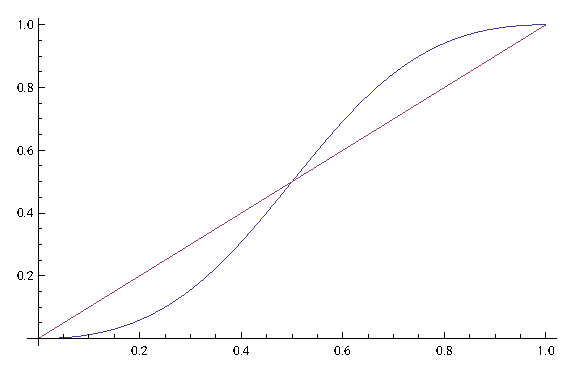
\includegraphics[width=0.9\textwidth]{figures/preferenceprob.eps}
      \caption{偏好概率模型}\label{fig:preferenceprob}
  \end{minipage}
  \begin{minipage}[t]{0.49\linewidth}
      \centering
      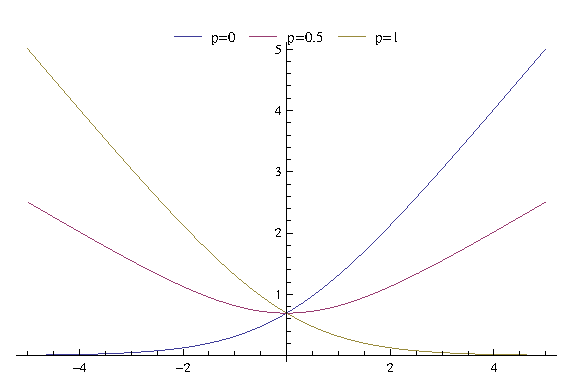
\includegraphics[width=0.9\textwidth]{figures/entropyloss.eps}
      \caption{交叉熵损失函数}\label{fig:entropyloss}
  \end{minipage}
\end{figure}

假设排序模型是连续函数$f:\mathbb{R}^m\mapsto \mathbb{R}$,对评分结果经过Logistic函数变换,可用于估计真实偏好概率:
\begin{equation}
    \widetilde{p}_{ij} = \frac{1}{1+e^{-o_{ij}}}
\end{equation}
其中,$o_{ij}=f(\theta,x_i)-f(\theta,x_j)$表示样本序对的预测差值。

排序模型预测结果同真实结果之间的差异可以使用概率分布的交叉熵距离表示,并直接用于度量排序模型在样本序对$(x_i,x_j)$上的预测损失
\begin{equation}
    \begin{array}{lll}
      L_{ij} & = & -\big[p_{ij} \log \widetilde{p}_{ij} + (1-p_{ij}) \log (1-\widetilde{p}_{ij})\big] \\
       & = & p_{ij} \log(1+e^{-o_{ij}}) + (1-p_{ij}) \log(1+e^{o_{ij}}) \\
       & = & \log(1+e^{o_{ij}}) - p_{ij} o_{ij}
    \end{array}
\end{equation}

交叉熵损失函数$L_{ij}$与真实偏好概率$p_{ij}$密切相关(见图\ref{fig:entropyloss}),偏好概率$p_{ij}$取值不同,损失函数随预测差值的变化趋势也不同。当$p_{ij}=0.5$ 时,表明样本序对的真实排名相同,损失函数关于样本序对的预测差值$o_{ij}$对称。当$o_{ij}=0$时损失量最小$L_{ij}=\log 2$,仍大于零。

\subsection{训练}
RankNet算法使用一个三层神经网络表示排序模型
\begin{equation}
    f(\theta,x) = \varphi \Big(b + \sum\limits_{l=1}^h \upsilon_l \phi_l\big(b_l + \sum\limits_{k=1}^m \omega_{kl} x_k\big)\Big)
\end{equation}
其中,输入层有$m$个输入节点,隐藏层有$h$个节点,输出层只有一个输出节点。隐藏层的刺激函数为$\phi_1,\ldots,\phi_h$,输出层的刺激函数$\varphi$,均为Sigmoid函数。$b_1,\ldots,b_h$与$b$都是偏置量。参数$\omega_{kl}$表示第$k$个输入节点到第$l$个隐藏节点的连接权值,$\upsilon_l$则是第$l$个隐藏节点到输出节点的权值。$x_k$表示输入向量$x$的第$k$个元素。

\begin{algorithm}[htbp]
        \caption{RankNet算法}
        \begin{algorithmic}
            \REQUIRE ~~训练集$\{(x_i,x_j),p_{ij},(i,j)\in \mathscr P\}$,学习率$\eta$,迭代次数$T$,初始网络参数$\theta_0$ \\
            \FOR{$t = 1,\dots, T$}
                \FOR{对任意的$(i,j)\in \mathscr P$}
                \STATE
                \begin{enumerate}
                  \item 前向传播:以$(x_i,x_j)$为输入,计算当前网络的输出值
                  \[
                    \begin{array}{l}
                      f_i=f(\theta_{t-1},x_i) \\
                      f_j=f(\theta_{t-1},x_j)
                    \end{array}
                  \]
                  \item 反向传播:使用梯度下降法更新网络参数
                  \[
                    \theta_t = \theta_{t-1} - \eta \nabla L_{ij}
                  \]
                \end{enumerate}
                \ENDFOR
            \ENDFOR
            \ENSURE ~~排序模型$f(\theta_T,x)$
        \end{algorithmic}
\end{algorithm}

RankNet算法使用样本训练集$\{x_i,y_i\}_{i=1}^n$上的偏好序对
\begin{equation}
    \mathscr P = \{(i,j)\mid y_i \ge y_j, i,j=1,\ldots,n\}
\end{equation}
作为网络模型训练样本的索引集,每次训练时从训练集中选取一对样本$(x_i,x_j)$作为输入,通过\textbf{前向传播}(Forward Propagation)在整个网络扩散,产生一对网络输出$(f(\theta,x_i),f(\theta,x_j))$。

假设网络模型的刺激函数都是连续可微的,可以计算网络模型$f(\theta,x)$交叉熵损失函数的梯度
\begin{equation}\label{eq:ranknet-gradient}
    \nabla_{\theta} L_{ij} = \frac{\partial L_{ij}}{\partial o_{ij}} [\nabla_{\theta} f_i- \nabla_{\theta} f_j]
\end{equation}
其中,$f_i=f(\theta,x_i),f_j=f(\theta,x_j)$。根据$f_i$关于$b,\upsilon_l,b_l,\omega_{kl}$的一阶导数
\begin{equation}
    \left\{
    \begin{array}{l}
      \nabla_b f_i = \varphi'(\theta,x_i) \equiv \nabla_1^{(i)} \\
      \nabla_{\upsilon_l} f_i = \varphi'(\theta,x_i) \phi_l(b_l,\omega,x_i) = \nabla_1^{(i)}  \phi_l(b_l,\omega,x_i) \\
      \nabla_{b_l} f_i = \varphi'(\theta,x_i) \upsilon_l \phi'_l(b_l,\omega,x_i) = \nabla_1^{(i)} \upsilon_l \phi'_l(b_l,\omega,x_i) \equiv \nabla_2^{(i)} \\
      \nabla_{\omega_{kl}} f_i = \varphi'(\theta,x_i) \upsilon_l \phi'_l(b_l,\omega,x_i) x_{ik} = \nabla_2^{(i)} x_{ik}
    \end{array}
    \right.
\end{equation}
可以推导得到损失函数$L_{ij}$的梯度:
\begin{equation}
    \left\{
    \begin{array}{l}
      \nabla_b L_{ij} = L'_{ij} \big[\nabla_1^{(i)} - \nabla_1^{(j)}\big]\\
      \nabla_{\upsilon_l} L_{ij} = L'_{ij} \big[\nabla_1^{(i)}  \phi_l(b_l,\omega,x_i) - \nabla_1^{(j)}  \phi_l(b_l,\omega,x_j)\big] \\
      \nabla_{b_l} L_{ij}= L'_{ij} \big[\nabla_2^{(i)} - \nabla_2^{(j)}\big] \\
      \nabla_{\omega_{kl}} L_{ij} = L'_{ij} \big[\nabla_2^{(i)} x_{ik} - \nabla_2^{(j)} x_{jk}\big] \\
    \end{array}
    \right.
\end{equation}

观察可以发现,神经网络中参数更新的方向是从输出层开始逐层往后直至输入层,这种根据梯度下降法更新参数的流程因此称作\textbf{反向传播}(Backward Propagation):
\begin{equation}
    \theta \leftarrow \theta - \eta \nabla L_{ij}
\end{equation}
其中,$\eta$表示学习率。

在训练模型时,RankNet采用了一种简化的概率化规则
\begin{equation}
    p_{ij} = \left\{
        \begin{array}{ll}
          1 & y_i > y_j \\
          0.5 & y_i = y_j \\
        \end{array}
    \right.
\end{equation}

\subsection{批量更新}
原始的RankNet算法使用的是随机梯度下降法,每次更新网络模型参数的粒度都是单个样本对,梯度计算的复杂度是$\complex(N^2)$,其中$N$ 表示平均每个检索词的关联文档数目。2007年,Burges等人\cite{burges2007learning}在原始RankNet算法的基础上设计出一种高效的训练方法,他们提出将梯度计算的中间结果保存再利用,使用累加形式的梯度值对参数一次性更新,参数更新的粒度是检索词层面。这种方法由此称为\textbf{批量梯度下降法},计算复杂度仅为$\complex(N)$。

\begin{algorithm}[htbp]
        \caption{批量更新版RankNet算法}
        \begin{algorithmic}
            \REQUIRE ~~训练集${Q,\mathcal{X},\mathcal{Y}}$,学习率$\eta$,迭代次数$T$,初始网络参数$\theta_0$ \\
            \FOR{$t = 1,\dots, T$}
            \FOR{任意的检索词$q\in Q$}
                \FOR{检索词$q$的任意关联文档$x$}
                \STATE 前向传播:以$x$为输入,计算并保存所有隐藏节点与输出节点的输出值
                \ENDFOR
                \STATE 反向传播:使用批量梯度下降法更新网络参数
                \[
                  \theta_t = \theta_{t-1} - \eta \sum\limits_i \Big(\lambda_i \frac{\partial f_i}{\partial \theta}\Big)\Big|_{\theta_{t-1}}
                \]
            \ENDFOR
            \ENDFOR
            \ENSURE ~~排序模型$f(\theta_T,x)$
        \end{algorithmic}
\end{algorithm}

网络模型在所有样本序对$\mathscr P$上的预测损失可以表示成一种加和形式
\begin{equation}
    L = \sum\limits_{(i,j)\in \mathscr P} L_{ij}
\end{equation}

对于单个样本序对$(x_i,x_j)$,我们使用$L_{ij}$关于函数值$f_i,f_j$的导数可以推知:
\begin{equation}\label{eq:ranknet-batchgradient}
    \frac{\partial L}{\partial \theta} = \sum\limits_{(i,j)\in \mathscr P} \big(\frac{\partial L_{ij}}{\partial f_i} \frac{\partial f_i}{\partial \theta} + \frac{\partial L_{ij}}{\partial f_j} \frac{\partial f_j}{\partial \theta} \big)
\end{equation}

为方便记,我们定义两个指标集$\mathscr P_{i*}$与$\mathscr P_{*i}$:
\begin{equation}
    \mathscr P_{i*} = \{j\mid (i,j)\in \mathscr P\}~~,~~\mathscr P_{*i} = \{j\mid (j,i)\in \mathscr P\}
\end{equation}

索引集可以拆分如下:
\begin{equation}
    \sum\limits_{(i,j)\in \mathscr P} = \sum\limits_{i=1}^n \sum\limits_{j\in \mathscr P_{i*}} = \sum\limits_{j=1}^n \sum\limits_{i\in \mathscr P_{*j}}
\end{equation}

根据索引集的拆分形式,重新整理等式\eqref{eq:ranknet-batchgradient}可得
\begin{equation}
    \begin{array}{lll}
     \frac{\partial L}{\partial \theta} & = & \sum\limits_i \sum\limits_{j\in \mathscr P_{i*}} \frac{\partial L_{ij}}{\partial f_i} \frac{\partial f_i}{\partial \theta} + \sum\limits_j \sum\limits_{i\in \mathscr P_{*j}} \frac{\partial L_{ij}}{\partial f_j}\frac{\partial f_j}{\partial \theta} \\
     & = & \sum\limits_i \frac{\partial f_i}{\partial \theta} \sum\limits_{j\in \mathscr P_{i*}} \frac{\partial L_{ij}}{\partial f_i} + \sum\limits_j \frac{\partial f_j}{\partial \theta}  \sum\limits_{i\in \mathscr P_{*j}} \frac{\partial L_{ij}}{\partial f_j} \\
     & = & \sum\limits_i \frac{\partial f_i}{\partial \theta} \big[\sum\limits_{j\in \mathscr P_{i*}} \frac{\partial L_{ij}}{\partial f_i} + \sum\limits_{j\in \mathscr P_{*i}} \frac{\partial L_{ji}}{\partial f_i}\big]
    \end{array}
\end{equation}
对于每个数据样本$x_i$,经过网络模型的一次前向传播计算其输出分值$f_i$,并且每个样本都涉及两个加和形式的梯度运算
\begin{equation}
    \lambda_i = \sum\limits_{j\in \mathscr P_{i*}} \frac{\partial L_{ij}}{\partial f_i} + \sum\limits_{j\in \mathscr P_{*i}} \frac{\partial L_{ji}}{\partial f_i},~~i=1,\ldots,n
\end{equation}
两个加和项的计算量与数据样本相关等级数目、每个相关等级的文档数目有关,相对计算量较小。每个数据样本最后都需要计算一个关于参数$\theta$梯度值。

\section{LambdaRank}
排名标准度量指标通常是非平滑的,对直接优化形成阻碍。对此,在机器学习领域,有两种常用的间接优化的方法:确定标准度量指标的平滑边界函数或者近似函数,通过优化边界函数或近似函数,实现间接优化标准度量指标的目的。无论是界函数还是近似函数都与真实的标准度量指标存在一定的差距,间接优化的结果与真实最优解不一致性。

2007年,Burges等人\cite{burges2007learning}分析排序性能、损失函数及样本序对排名间的关系,巧妙地避开非平滑函数梯度的计算,直接构造具有期望性质的梯度函数(Lamda函数类),并将这种思想应用到RankNet算法,基于非平滑的标准度量指标(NDCG)训练排序模型。他们直接定义了损失函数关于预测结果的梯度,并使用希腊字母$\lambda$表示,所设计的算法由此称为LambdaRank。

\section{LambdaMART}
2010年,Burges\cite{burges2010from,ganjisaffar2011bagging}使用梯度提升决策树(Gradient Boost Decision Tree,也称MART),训练排序模型,在LambdaRank 算法的基础上,发展成为高效的LambdaMART算法,并一举赢得Yahoo!排序学习挑战赛(Learning To Rank Challenge)第一轮比赛。LambdaRank算法改进于RankNet算法,都是基于神经网络构建的排序模型,而LambdaMART基于回归决策树,可视为决策树版本的LambdaRank算法。

\section{GBRank}
\cite{zheng2007regression}A Regression Framework for Learning Ranking Functions Using Relative Relevance Judgments

\section{GBlend}
Learning to Blend by Relevance\cite{chen2010learning}

\section{QBRank}
A General Boosting Method and its Application to Learning Ranking Functions for Web Search\cite{zheng2007general}

\section{ListNet}
2007年,Cao等人\cite{cao2007learning}提出的ListNet是第一个序列型排序学习方法,比逐点型、序列型排序学习方法性能优越。ListNet算法根据Plackett-Luce模型,从排序模型预测的分值列表中计算排列概率分布(Permutation Probability Distribution),将文档真实标记作为文档分值,据此计算真实概率分布。ListNet定义了排序模型预测的概率分布与真实概率分布之间的交叉熵损失函数,利用梯度下降法最小化损失函数,达到优化排序模型的目的。

\begin{definition}[排列概率]
假设$\Pi[n]$表示由$n$个对象所有可能排列构成的集合,由对象分值列表$Y$生成排列$\pi\in\Pi_n$的概率定义如下:
\[
    P(\pi|Y) = \prod\limits_{i=1}^n \frac{\phi(y_{\pi^{-1}(i)})}{\sum\limits_{k=i}^n \phi(y_{\pi^{-1}(k)})},
\]
其中$y_{\pi^{-1}(i)}$表示$\pi$中排第$i$位的对象$\pi^{-1}(i)$的分值,$\phi>0$是一个单调递增函数。这种模型称作\textbf{Luce模型},其复杂度是$\complex(n!)$,当$n$ 增加,会产生巨大的计算开销。
\end{definition}
文档排名问题主要目标是确保“排名越靠前越相关”,我们来看排名前$K$的对象排列分布。
\begin{definition}[TopK概率]
对于给定的$K<n$,我们如果只关注排名前$K$的对象,由对象分值列表$Y$生成排列$\pi\in \Pi[n]$的概率定义如下:
\[
    P(\pi|Y;K) = \prod\limits_{i=1}^K \frac{\phi(y_{\pi^{-1}(i)})}{\sum\limits_{k=i}^n \phi(y_{\pi^{-1}(k)})}.
\]
其复杂度是$\complex(n^K)$,只需要计算$n!/(n-K)!$次,远远小于$n!$。
\end{definition}

ListNet算法使用的是最简的Top-1概率,根据定义由对象分值列表$Y$生成排列$\pi$的Top-1概率可表示如下
\[
    P(\pi|Y;1) = \frac{\phi(y_{\pi^{-1}(1)})}{\sum\limits_{k=1}^n \phi(y_{\pi^{-1}(k)})}.
\]
假设$\hat Y=f(X;\Theta)$是模型$f$对训练样本的相关性预测评分列表,$Y$是训练样本的真实相关性评分列表,ListNet算法使用$P(\pi|\hat Y;1)$近似表示$P(\pi|\hat Y)$,使用$P(\pi|Y;1)$ 近似表示$P(\pi|Y)$,通过最小化交叉熵损失函数
\[
    L(X,Y;\Theta) = -\sum\limits_{\pi^{-1}(1) = 1}^n P(\pi|Y;1) \log P(\pi|\hat Y;1)
\]
训练预测模型参数$\Theta$。

\section{ListMLE}
2008年,Xia等人\cite{xia2008listwise}从损失函数的一致性出发,提出一个新的序列型排序学习算法ListMLE。它是ListNet的一个拓展,也是通过神经网络,应用梯度下降法最小化损失函数,训练出最优排名函数。两者都是建立在Plackett-Luce概率模型之上的序列型排序学习方法,但是使用的损失函数不同,ListNet使用的是交叉熵损失函数,而ListMLE使用的则是似然损失函数。

假设$Y$是训练样本的真实相关性评分列表,根据真实相关性评分从高到低排序,可以生成一个排列$\pi$。ListMLE方法利用TopK概率模型,定义损失函数为对数似然函数
\[
    L(X,Y; \Theta) = -\log P(\hat Y|X; \Theta) = -\log \prod\limits_{i=1}^K \frac{\phi(f(x_{\pi^{-1}(i)};\Theta))}{\sum\limits_{k=i}^n \phi(f(x_{\pi^{-1}(k)};\Theta))}.
\]

\section{FRank}
FRank: A Ranking Method with Fidelity Loss\cite{tsai2007frank}

\section{BoltzRank}
BoltzRank: Learning to maximize expected ranking gain\cite{volkovs2009boltzrank}

\section{SortNet}
SortNet: learning to rank by a neural-based sorting algorithm\cite{rigutini2008sortnet}

\section{RankBoost}
2003年,Freund等人提出了RankBoost方法\cite{freund2003efficient},其基本思想源于AdaBoost\cite{freund1995desicion,schapire1999improved}。它根据排序模型在样本序对上的预测误差,训练多个弱排名函数$h_t$,并加权形成组合排序模型
\[f_T = \sum\limits_{t=1}^T \alpha_t h_t,\]
$\alpha_t$表示弱排名模型$h_t$的权重。

RankBoost使用反馈函数以真实地反映文档序关系,根据样本的原始分值对样本序对重新标记,作为序对型训练样本的真实标记,并定义一种分类误差最小化的排名损失函数,期望训练得到的模型的预测结果与反馈结果尽可能地一致。RankBoost是首个Boosting框架下用于排序问题的学习算法,属于序对型排序学习方法,可应用于元搜索引擎排名聚合、协同过滤推荐系统等。RankBoost算法可以概括如下:

\begin{algorithm}[htbp]
        \caption{RankBoost学习算法}
        \begin{algorithmic}
            \REQUIRE ~~训练集$S=\{q_i,x_i,y_i\}^m_{i=1}$,迭代次数$T$,特征集合$\varPhi$\\
            \STATE
            \begin{itemize}
              \item 在训练集上对每个检索词构建一组序对集$\mathscr P_i = \{(x_1, x_2)\mid y_1 > y_2\}$,初始化序对样本$X\times X$上的概率分布$D_1$
            \end{itemize}
            \FOR{$t = 1,\dots, T$}
            \STATE
            \begin{enumerate}
              \item 基于样本序对的概率分布$D$训练弱排序模型$h_t:X\mapsto \mathbb{R}$
              \item 给弱排序模型赋权值$\alpha_t \in \mathbb{R}$
              \item 更新概率分布
              \begin{equation}
                D_{t+1}(x_1,x_2) = D_t(x_1,x_2) \frac{\exp\big\{-\alpha_t \big[h_t(x_1) - h_t(x_2)\big]\big\}}{Z_t}
              \end{equation}
              其中,$Z_t$是标准化因子。
            \end{enumerate}
            \ENDFOR
            \ENSURE ~~最终排名函数$f_T = \sum\limits_{t=1}^{T}{\alpha_t h_t}$
        \end{algorithmic}
\end{algorithm}

根据RankBoost的概率分布更新方式可知,如果$h_t$能够对$\mathscr P$中的文档序对给出正确的排名,也就是说当$h_t(x_1) - h_t(x_2)>0$,由于$\alpha_t>0$,相应地需要降低该序对在下轮迭代中的权重;否则,增大权重。这个特征与Boosting技术精神是吻合的。

\subsection{排名误差}
对于RankBoost的排名误差,可以证明“\textbf{最终排名函数$f_T$在初始概率分布$D_1$下的排名误差有上界}”:
\begin{equation}
    L_{D_1}(f_T) \le \prod_{t=1}^T Z_t
\end{equation}
我们下面给出简要证明。

\begin{proof}
根据排名误差的定义:
\begin{equation}
    L_{D_1}(f_T) = \sum\limits_{(x_1,x_2)\in \mathscr P} D_1(x_1,x_2) I(f_T(x_1) \le f_T(x_2)) \le \sum\limits_{(x_1,x_2)\in \mathscr P} D_1(x_1,x_2) \exp(-[f_T(x_1) - f_T(x_2)])
\end{equation}

由概率分布更新策略可知:
\begin{equation}
  D_{t+1}(x_1,x_2) = D_t(x_1,x_2) \frac{\exp\big\{-\alpha_t \big[h_t(x_1) - h_t(x_2)\big]\big\}}{Z_t}
\end{equation}

将其在$T+1$处展开可得:
\begin{equation}
    \begin{array}{lll}
      D_{T+1}(x_1,x_2) & = & D_1(x_1,x_2) \prod\limits_{t=1}^T \exp\big\{-\alpha_t \big[h_t(x_1) - h_t(x_2)\big]\big\}/\prod\limits_{t=1}^T  Z_t \\
       & = & D_1(x_1,x_2) \exp\big\{\sum\limits_{t=1}^T -\alpha_t \big[h_t(x_1) - h_t(x_2)\big]\big\}/\prod\limits_{t=1}^T  Z_t\\
       & = & D_1(x_1,x_2) \exp(-[f_T(x_1) - f_T(x_2)])/\prod\limits_{t=1}^T  Z_t
    \end{array}
\end{equation}

根据展开式,则
\begin{equation}
    L_{D_1}(f_T) \le \sum\limits_{(x_1,x_2)\in \mathscr P} D_{T+1} \prod\limits_{t=1}^T  Z_t = \prod\limits_{t=1}^T  Z_t,
\end{equation}
证毕。
\end{proof}

根据排名误差上界可以推断,如果在每轮迭代过程通过选择合适的弱学习器,并给其赋予恰当的权值,最小化标准化因子
\begin{equation}
    Z_t = \sum\limits_{(x_1,x_2)\in \mathscr P} D_t(x_1,x_2)\exp\big\{-\alpha_t \big[h_t(x_1) - h_t(x_2)\big]\big\}
\end{equation}
则可以保证训练得到一个低排名误差的组合模型$f_T$。

\subsection{弱学习器选择和赋权}
根据上一小节的结论,弱学习器的选择与赋权的目标是最小化标准化因子:
\begin{equation}
    (\alpha_t, h_t) = \argmin\limits_{\alpha, h} \sum\limits_{(x_1,x_2)\in \mathscr P} D_t(x_1,x_2) \exp\big\{-\alpha \big[h(x_1) - h(x_2)\big]\big\}
\end{equation}

下面我们将重点介绍弱学习器选择与加权的基本思路。为方便记,在不引起混淆的情况,我们将省略掉变量下标$t$。

\textbf{给定弱学习器$h$},标准化因子是单变量$\alpha$的函数,使用简单的搜索算法即可确定其唯一的最小值点。对于特殊的弱学习器,比如二元函数$h\in\{0,1\}$ ,定义
\begin{equation}
    W_b = \sum\limits_{(x_1,x_2)\in \mathscr P} D(x_1,x_2) I(h(x_1) - h(x_2) = b)
\end{equation}
则$b\in\{-1,0,1\}$,根据定义,$W_{+1}$表示能够被$h$正确排序的文档序对权重,类似地,$W_{-1}$则等于被$h$错误排列的文档序对权重。

利用$W_b$改写标准化因子:
\begin{equation}
    Z(\alpha)= \sum\limits_{(x_1,x_2)\in \mathscr P} D(x_1,x_2) \exp\big\{-\alpha \big[h(x_1) - h(x_2)\big]\big\} = W_{-1} e^{\alpha} + W_0 + W_{+1} e^{-\alpha}
\end{equation}

根据极值条件可以推得
\begin{equation}
    \frac{dZ}{d\alpha} = W_{-1} e^{\alpha} - W_{+1} e^{-\alpha} = 0
\end{equation}
成立,$Z(\alpha)$的最小值点为
\begin{equation}
    \hat\alpha = \frac{1}{2} \log(\frac{W_{+1}}{W_{-1}})
\end{equation}
如果$W_{+1}\ge W_{-1}$,则$\hat\alpha\ge 0$;否则,$\hat\alpha< 0$。

将最小值点$\hat\alpha$带入标准化因子
\begin{equation}\label{eq:optimalbinaryclassifier}
    Z(\hat\alpha) = W_0 + 2\sqrt{W_{-1}W_{+1}}
\end{equation}

使用二元弱学习器$h\in\{0,1\}$对文档排名,实际上是将排序问题转化为二元分类问题,直接使用成熟的分类理论处理排名问题,适用范围受到极大的限制。我们下面将介绍另外一种常见的形式:$h\in [0,1]$。

\textbf{给定弱学习器$h\in [0,1]$},我们利用$Z$的近似(界)确定$h$的最优权值$\alpha$。根据$e^{\alpha x}$的凸性可知,如果$x\in[0,1]$,则有下式
\begin{equation}
    e^{\alpha x} \le \frac{1 + x}{2} e^{\alpha} + \frac{1 - x}{2} e^{-\alpha}
\end{equation}
成立。对于$Z(\alpha)$
\begin{equation}
    \begin{array}{lll}
      Z(\alpha) & = & \sum\limits_{(x_1,x_2)\in \mathscr P} D(x_1,x_2) \exp\big\{-\alpha \big[h(x_1) - h(x_2)\big]\big\} \\
       & \le & \sum\limits_{(x_1,x_2)\in \mathscr P} \bigg[D(x_1,x_2) \frac{1 - \big[h(x_1) - h(x_2)\big]}{2} e^{\alpha} + \frac{1 + \big[h(x_1) - h(x_2)\big]}{2} e^{-\alpha}\bigg] \\
       & = & (\frac{1 - \varphi}{2}) e^{\alpha} + (\frac{1 + \varphi}{2}) e^{-\alpha} \\
       & \triangleq & \widetilde{Z}(\alpha)
    \end{array}
\end{equation}
其中,
\begin{equation}
    \varphi = \sum\limits_{(x_1,x_2)\in \mathscr P} D(x_1,x_2) \big[h(x_1) - h(x_2)\big]
\end{equation}
表示弱学习器对$x_1$与$x_2$预测结果的期望间隔。

我们通过最小化$Z(\alpha)$的上界函数$\widetilde{Z}(\alpha)$,达到间接优化$Z(\alpha)$的目的。根据极值条件
\begin{equation}
    \frac{d\widetilde{Z}(\alpha)}{d\alpha} = (\frac{1 - \varphi}{2}) e^{\alpha} - (\frac{1 + \varphi}{2}) e^{-\alpha} = 0
\end{equation}
可以求得最小值点
\begin{equation}
    \hat\alpha = \frac{1}{2} \ln \frac{1+\varphi}{1-\varphi}
\end{equation}
从而可得最优标准化因子
\begin{equation}
    Z(\hat\alpha) \le \sqrt{1-\varphi^2}
\end{equation}

为了实现近似最小化$Z$,根据以上推导过程,我们选择能够最大化$|\varphi|$的弱学习器,即:
\begin{equation}\label{eq:optimalweakselect}
    \hat h = \argmax_{h} |\varphi| = \argmax\limits_{h} \bigg|\sum\limits_{(x_1,x_2)\in \mathscr P} D(x_1,x_2) \big[h(x_1) - h(x_2)\big]\bigg|
\end{equation}
这正是RankBoost所采用的弱学习器选择与赋权方案:通过最大化期望间隔选择弱学习器,实现近似最小化标准化因子进而最小化排序损失给弱学习器赋权。

\subsection{弱学习器的构造}
无论是弱学习选择还是赋权都是基于指定类型的弱学习器,必然会涉及到弱学习器的构造问题。本节主要讨论弱学习器之弱排序模型的构造方法。

构造弱排名函数$h$最简单也是最明了的方法是使用样本的单个排名特征$f_i$作为排名函数,然而此法的薄弱之处在排名特征对真实分值的过分依赖
\cite{freund2003efficient},在诸如排名聚合之类的应用中,我们无从得知各自的真实分值,并且不同搜索引擎所采用的评分算法不同,纵然知晓具体分值,也不能直接使用。对于任意类型的搜索引擎,从搜索结果中我们能够获得的最具价值、最宜标准化的信息是关联文档的相对序关系,而且更易推广,适用性也更强。鉴于此,我们主要关注基于\textbf{相对序关系信息}构造弱排名函数。

\cite{freund2003efficient}声称在构造弱排名函数时,忽略排名特征的具体分值,仅使用排名特征提供的排序信息。实际上,弱排名函数是依赖于具体分值$f_i(x)$同一个阈值$\theta$比较结果:
\begin{equation}\label{eq:weakconstruct}
    h(x) = \left\{
        \begin{array}{ll}
          1 & f_i(x) > \theta \\
          0 & f_i(x) \le \theta \\
          q & f_i(x) = \bot
        \end{array}
    \right.
\end{equation}
其中,$\theta$,$q\in\{0,1\}$是优化选择的参数,而$f_i(x) = \bot$表示排名特征为获取$x$的任何信息。

根据弱排名函数的选择与赋权分析流程,如果通过优化\eqref{eq:optimalbinaryclassifier}选择弱排名函数时间复杂度是$\complex(n|\varPhi||\chi_{\varPhi}|)$。如果通过优化\eqref{eq:optimalweakselect}选择弱排名函数,可以通过变换合并$\varphi$各项,从而减少时间复杂度至$\complex(|\varPhi|)$:
\begin{equation}
    \begin{array}{lllc}
      \varphi & = & \sum\limits_{(x_1,x_2)\in \mathscr P} D(x_1,x_2) \big[h(x_1) - h(x_2)\big] \\
       & = & \sum\limits_{(x_1,x_2)\in \mathscr P} D(x_1,x_2) h(x_1) - \sum\limits_{(x_1,x_2)\in \mathscr P} D(x_1,x_2) h(x_2) \\
       & = & \sum\limits_{x_1} h(x_1) \sum\limits_{x_2\in \mathscr P_{1*}} D(x_1,x_2) -  \sum\limits_{x_2} h(x_2) \sum\limits_{x_1\in \mathscr P_{*2}} D(x_1,x_2) \\
       & = & \sum\limits_{x_1} h(x_1) \sum\limits_{x_2\in \mathscr P_{1*}} D(x_1,x_2) -  \sum\limits_{x_1} h(x_1) \sum\limits_{x_2\in \mathscr P_{*1}} D(x_2,x_1) \\
       & = & \sum\limits_{x_1} h(x_1) \big[\sum\limits_{x_2\in \mathscr P_{1*}} D(x_1,x_2) - \sum\limits_{x_1\in \mathscr P_{*2}} D(x_2,x_1)\big]\\
       & = & \sum\limits_{x} h(x) \big[\sum\limits_{x\succ x'} D(x,x') - \sum\limits_{x'\succ x} D(x',x)\big]\\
       & = & \sum\limits_{x} h(x) \pi(x)\\
    \end{array}
\end{equation}
其中,$\pi(x) = \sum\limits_{x\succ x'} D(x,x') - \sum\limits_{x'\succ x} D(x',x)$。对于排名特征$f_i$,如果将$h(x)$的表达式带入$\varphi$,可得:
\begin{equation}
    \varphi = \sum\limits_{x:f_i(x)> \theta} \pi(x) + q \sum\limits_{x:f_i(x)= \bot} \pi(x)
\end{equation}

根据$\pi(x)$的定义可知$\sum\limits_{x} \pi(x) = \sum\limits_{x} \sum\limits_{x\succ x'} D(x,x') - \sum\limits_{x'\succ x} D(x',x) = 0$,故而:
\begin{equation}
    \sum\limits_{x:f_i(x)= \bot} \pi(x) = - \sum\limits_{x:f_i(x)\ne \bot} \pi(x)
\end{equation}
$\varphi$可以进一步化简得:
\begin{equation}
    \varphi = \sum\limits_{x:f_i(x)> \theta} \pi(x) - q \sum\limits_{x:f_i(x)\ne \bot} \pi(x) = \mathbb{L} - q\mathbb{R}
\end{equation}
在学习弱排名函数时,遍历特征集$f \in\{f_i\}_{i=1}^n$,阈值列表$\theta\in\{\theta_j\}_{j=1}^J$,计算$\mathbb{L},\mathbb{R}$,选择一个局部最优的$q\in\{0,1\}$,计算$\varphi$,从而优选出全局最优的参数组合。

\subsection{二分反馈}
本小节主要考察一种特殊的反馈函数——二分反馈(Bipartite Feedback):在$X$上存在两个不相交的子集$X_1,X_2$,如果对于任意的$x_1\in X, x_2\in X$,反馈函数定义成下面的形式:
\begin{equation}
    \varPhi(x_1,x_2) = \left\{
        \begin{array}{cl}
          -1, &  x_1\in X_2, x_2\in X_1, \\
           1,  &  x_1\in X_1, x_2\in X_2, \\
           0,  &  x_1\ni X_1|x_2\ni X_2,
        \end{array}
    \right.
\end{equation}
则用于表达偏好关系的反馈函数$\varPhi$是二分反馈。二分反馈可以很容易的推广到一般类型的反馈。
%在信息检索领域,排名较之分类更有价值:排名反映了算法的预测的置信程度,用户没有耐心或充足的时间从大量相关文档中挑选合口味的文档。

\begin{algorithm}[htbp]
        \caption{RankBoost二分反馈学习算法}
        \begin{algorithmic}
            \REQUIRE ~~训练集$X$上不相交的子集$X_1,X_2$,迭代次数$T$\\
            \STATE
            \begin{itemize}
              \item 初始化样本分布
              \begin{equation}
                \omega_1(x) = \left\{
                    \begin{array}{ll}
                      1/|X_1| & ,  x\in X_1 \\
                      1/|X_2| & ,  x\in X_2
                    \end{array}
                \right.
              \end{equation}
              \item 根据样本权值概率分布,初始化样本序对分布$D_1(x_1,x_2) = \omega_1(x_1)\omega_1(x_2)$
            \end{itemize}
            \FOR{$t = 1,\dots, T$}
            \STATE
            \begin{enumerate}
              \item 基于样本序对的概率分布$D_t(x_1,x_2) = \omega_t(x_1)\omega_t(x_2)$训练弱排序模型$h_t:X\mapsto \mathbb{R}$
              \item 给弱排序模型赋权$\alpha_t \in \mathbb{R}$
              \item 更新概率分布
              \begin{equation}
                \omega_{t+1}(x) = \left\{
                    \begin{array}{ll}
                       \omega_t(x)\dfrac{\exp(\alpha_t h_t(x))}{Z_t^1} & , x\in X_1\\
                       \omega_t(x)\dfrac{\exp(-\alpha_t h_t(x))}{Z_t^2} & , x\in X_2
                    \end{array}
                \right.
              \end{equation}
              其中,$Z_t^i$是$X_i$上的标准化因子($i=1,2$):
              \begin{equation}
                \left\{
                \begin{array}{lll}
                  Z_t^1 & = & \sum\limits_{x\in X_1} \omega_t \exp(\alpha_t h_t(x))\\
                  Z_t^2 & = & \sum\limits_{x\in X_2} \omega_t \exp(-\alpha_t h_t(x))\\
                \end{array}
                \right.
              \end{equation}
            \end{enumerate}
            \ENDFOR
            \ENSURE ~~最终排名函数$f_T = \sum\limits_{t=1}^{T}{\alpha_t h_t}$
        \end{algorithmic}
\end{algorithm}

如果令$Z_t = Z_t^1 \cdot Z_2^2$,可以推导它等价于一般形式的标准化因子:
\begin{equation}
    \begin{array}{lll}
      D_{t+1}(x_1,x_2) & = & D_t(x_1,x_2) \frac{\exp\big\{-\alpha_t \big[h_t(x_1) - h_t(x_2)\big]\big\}}{Z_t} \\
       & = & \omega_t(x_1)\frac{\exp(\alpha_t h_t(x_1))}{Z_t^1} \cdot \omega_t(x_2)\frac{\exp(\alpha_t h_t(x_2))}{Z_t^2}\\
       & = & \omega_{t+1}(x_1)\omega_{t+1}(x_2)
    \end{array}
\end{equation}

在二分反馈形式的RankBoost算法中,若选择最佳的弱学习器,需要最大化$\varphi$,我们充分利用二分反馈的特点,重新改写$\varphi$:
\begin{equation}
    \begin{array}{lll}
      \varphi & = & \sum\limits_{(x_1,x_2)\in \mathscr P} D(x_1,x_2) \big[h(x_1) - h(x_2)\big] \\
       & = & \sum\limits_{(x_1,x_2)\in \mathscr P} \omega(x_1)\omega(x_2) \big[h(x_1) - h(x_2)\big] \\
       & = & \sum\limits_{(x_1,x_2)\in \mathscr P} \omega(x_1)\omega(x_2) h(x_1) - \sum\limits_{(x_1,x_2)\in \mathscr P} \omega(x_1)\omega(x_2) h(x_2) \\
       & = & \sum\limits_{x_1\in X_1} \omega(x_1)h(x_1) \sum\limits_{x_2\in X_2} \omega(x_2) - \sum\limits_{x_2\in X_2} \omega(x_2)h(x_2) \sum\limits_{x_1\in X_1} \omega(x_1)
    \end{array}
\end{equation}
为方便记,我们引入新的变量:
\begin{equation}
    s(x) = \left\{
        \begin{array}{l}
          +1, x \in X_1\\
          -1, x \in X_2
        \end{array}
    \right.
\end{equation}
故而:
\begin{equation}
    \begin{array}{lll}
      \varphi & = & \sum\limits_{x_1\in X_1} s(x_1)\omega(x_1)h(x_1) \sum\limits_{x_2\in X_2} \omega(x_2) + \sum\limits_{x_2\in X_2} s(x_2) \omega(x_2)h(x_2) \sum\limits_{x_1\in X_1} \omega(x_1) \\
      & = & \sum\limits_{x} \bigg[s(x)\omega(x)h(x) \sum\limits_{x':s(x') = -s(x)} \omega(x')\bigg]
    \end{array}
\end{equation}
二分反馈的计算优势是明显的,可以将计算复杂度从$\complex(|X_1|\cdot|X_2|)$降低至$\complex(|X_1| + |X_2|)$。

\subsection{泛化误差}
这一小节,我们基于二元排序模型$h\in\{0,1\}$与二分反馈函数$\varPhi$确立组合排序模型的泛化界。假设$\varPhi$将样本空间$\mathcal{X}$分成两个互不相交的部分$X, Z$,使得对任意的$x\in X, z\in Z$,都有$\varPhi(x,z) > 0$,即$X$中样本排名高于$Z$。

在机器学习理论中,通常假设在样本空间$\mathcal{X}$存在某个未知的分布,训练数据与测试数据均是独立同分布的样本集合。对于二分反馈排序模型,最容易想到的是假设样本序对独立同分布于$\mathcal{X}\times \mathcal{X}$上的某个分布$D$。实际上,训练集中样本序对独立性都得不到满足,因此需要另辟新径:假设在集合$X,Z$ 上各存在一个样本分布$D_1,D_2$,则原始训练集就是分别服从$D_1,D_2$的样本集合的并。%根据此假设,我们可以定义训练误差(经验误差)、期望测试误差与泛化误差。

由RankBoost算法所确定的组合排序模型$f_T(x) = \sum\limits_{t=1}^T \alpha_t h_t(x)$,通过分值对文档排名。为分析模型对样本序对的预测精度,我们定义
\begin{equation}
    H(x,z) = \sgn\bigg(\sum\limits_{t=1}^T \alpha_t h_t(x) - \sum\limits_{t=1}^T \alpha_t h_t(z)\bigg)
\end{equation}
其中,$h_t\in \mathcal{H}$,$H\in \mathcal{C}$。$\mathcal{H}$是二元函数类,$\mathcal{C}$是函数集。

如果$H(x,z)\ne 1$,则表明$H$在$(x,z)\in X\times Z$上产生预测误差,结合排序问题的概率模型,由此我们可定义$H$的泛化误差:
\begin{equation}
    \varepsilon(H) = \sum\limits_{(x,z)\in X\times Z} p(x, z) I(H(x,z)\ne 1) = \mathbb{E}\bigg[I(H(x,z)\ne 1)\bigg]
\end{equation}
可以证明泛化误差的定义与测试误差是一致的。对于测试样本集合$T_X\times T_Z$,$T_X=\{x_1,\ldots,x_p\}$,$T_Z=\{z_1,\ldots,z_p\}$,则$H$的期望测试误差如下:
\begin{equation}
    \begin{array}{lll}
      \mathbb{E}\bigg[\frac{1}{pq} \sum\limits_{i=1}^p\sum\limits_{j=1}^q I(H(x_i,z_j)\ne 1) \bigg] & = & \frac{1}{pq} \sum\limits_{i=1}^p\sum\limits_{j=1}^q \mathbb{E}\bigg[I(H(x_i,z_j)\ne 1)\bigg] \\
      & = & \frac{1}{pq} \sum\limits_{i=1}^p\sum\limits_{j=1}^q \sum\limits_{(x_i,z_j)\in T_X\times T_Z} p(x_i, z_j) \bigg[I(H(x_i,z_j)\ne 1)\bigg] \\
      & = & \frac{1}{pq} \sum\limits_{i=1}^p\sum\limits_{j=1}^q \varepsilon(H) \\
      & = & \varepsilon(H)
    \end{array}
\end{equation}

假设训练样本是$S_X\times S_Z$,$S_X=\{x_1,\ldots,x_m\}$,$S_Z=\{z_1,\ldots,z_n\}$,类似地可以给出$H$的训练误差:
\begin{equation}
    \hat{\varepsilon}(H) = \frac{1}{mn} \sum\limits_{i=1}^m \sum\limits_{j=1}^n I(H(x_i,z_j)\ne 1)
\end{equation}

\textbf{我们的目标}是证明:训练误差$\hat{\varepsilon}(H)$以很高的概率逼近于泛化误差$\varepsilon(H)$,意味着组合排序模型在训练集上的表现具有足够的代表性,无论学习算法选择何种组合排序模型,模型的训练误差都能够精确地估计其泛化误差。换言之,对任意$\eta>0$,都存在一个小量$\epsilon>0$使得:
\begin{equation}
    \begin{array}{ll}
       & p\big(\exists H\in \mathcal{C}:|\hat{\varepsilon}(H) - \varepsilon(H)| > \epsilon \big) \\
       = & p\bigg(\exists H\in \mathcal{C}:\bigg|\frac{1}{mn} \sum\limits_{i=1}^m \sum\limits_{j=1}^n I(H(x_i,z_j)\ne 1) - \sum\limits_{(x,z)\in X\times Z} p(x, z) I(H(x,z)\ne 1) \bigg| > \epsilon \bigg) \\
       \le & \eta
    \end{array}
\end{equation}
整理绝对值内的量可得:
\begin{equation}
    \begin{array}{ll}
       & \frac{1}{mn} \sum\limits_{i=1}^m \sum\limits_{j=1}^n I(H(x_i,z_j)\ne 1) - \sum\limits_{(x,z)\in X\times Z} p(x, z) I(H(x,z)\ne 1) \\
      = & \frac{1}{mn} \sum\limits_{i=1}^m \sum\limits_{j=1}^n I(H(x_i,z_j)\ne 1) - \sum\limits_{x\in X}\sum\limits_{z\in Z} p(x)p(z) I(H(x,z)\ne 1) \\
      = & \bigg[\frac{1}{mn} \sum\limits_{i=1}^m \sum\limits_{j=1}^n I(H(x_i,z_j)\ne 1) - \frac{1}{m} \sum\limits_{i=1}^m \sum\limits_{z\in Z} p(z) I(H(x_i,z)\ne 1)\bigg] \\
      + & \bigg[\frac{1}{m} \sum\limits_{i=1}^m \sum\limits_{z\in Z} p(z) I(H(x_i,z)\ne 1) - \sum\limits_{x\in X}\sum\limits_{z\in Z} p(x)p(z) I(H(x,z)\ne 1)\bigg]\\
      = & \frac{1}{m} \sum\limits_{i=1}^m \bigg[\frac{1}{n} \sum\limits_{j=1}^n I(H(x_i,z_j)\ne 1)-\sum\limits_{z\in Z} p(z) I(H(x_i,z)\ne 1)\bigg]\\
      + & \sum\limits_{z\in Z} p(z)\bigg[\frac{1}{m} \sum\limits_{i=1}^m I(H(x_i,z)\ne 1) -  \sum\limits_{x\in X} p(x) I(H(x,z)\ne 1) \bigg]\\
    \end{array}
\end{equation}

为了使用分类泛化误差的结果,我们定义$F:X\times Z \rightarrow \{0,1\}$,表示函数$H$给$(x,z)$的排序是否正确,即$F(x,z) = I(H(x,z)\ne 1)$,则我们可以重写上面的等式为:
\begin{equation}\label{eq:rankboostge}
    \frac{1}{m} \sum\limits_{i=1}^m \bigg[\frac{1}{n} \sum\limits_{j=1}^n F(x_i,z_j)-\sum\limits_{z\in Z} p(z) F(x_i,z)\bigg]\\
      +  \sum\limits_{z\in Z} p(z)\bigg[\frac{1}{m} \sum\limits_{i=1}^m F(x_i,z) -  \sum\limits_{x\in X} p(x) F(x,z) \bigg]\\
\end{equation}

给定$z\in Z$,则$F(x,z)$可以看做是一个单变量二元函数,假设$\mathcal{F}_z$表示所有给定$z$的二元函数类,则\eqref{eq:rankboostge}第二部分中$F$取自$\bigcup\limits_z \mathcal{F}_z$。根据Vapnik\cite{vapnik1982estimation},对于任意$\eta>0$,存在某个与训练集$S_X$大小$m$、错误概率$\eta$和函数类$\bigcup\limits_z \mathcal{F}_z$ 的VC维$d_1$有关的$\varepsilon_1(m,\eta,d_1)$,使得
\begin{equation}
    p\bigg(\exists F\in \bigcup\limits_z \mathcal{F}_z: \bigg|\frac{1}{m} \sum\limits_{i=1}^m F(x_i,z) -  \sum\limits_{x\in X} p(x) F(x,z) \bigg| > \varepsilon_1(m,\eta,d_1) \bigg) < \eta
\end{equation}
成立,其中:
\begin{equation}
    \varepsilon_1(m,\eta,d_1) = 2\sqrt{\frac{d_1(\ln(2m/d_1) + 1) - \ln(\eta/9)}{m}}
\end{equation}

对于\eqref{eq:rankboostge}第一部分,我们可以得到类似的结论:对于任意$\eta>0$,存在$\varepsilon_2(n,\eta,d_2)$,使得
\begin{equation}
    p\bigg(\exists F\in \bigcup\limits_{i=1}^m \mathcal{F}_{x_i}: \bigg|\frac{1}{n} \sum\limits_{j=1}^n F(x_i,z_j)-\sum\limits_{z\in Z} p(z) F(x_i,z) \bigg| > \varepsilon_2(n,\eta,d_2) \bigg) < \eta
\end{equation}
成立,其中:
\begin{equation}
    \varepsilon_2(n,\eta,d_2) = 2\sqrt{\frac{d_2(\ln(2n/d_2) + 1) - \ln(\eta/9)}{n}}
\end{equation}

对于给定的$z\in Z$:
\begin{equation}
    \begin{array}{lll}
      F(x,z) & = & I(H(x,z)\ne 1) \\
       & = & I\bigg(\sum\limits_{t=1}^T \alpha_t h_t(x) \le \sum\limits_{t=1}^T \alpha_t h_t(z)\bigg) \\
       & = & I\bigg(\sum\limits_{t=1}^T \alpha_t h_t(x) - b \le 0\bigg) \\
    \end{array}
\end{equation}
其中,$b=\sum\limits_{t=1}^T \alpha_t h_t(z)$是关于$z$的常数。Freund与Schapire\cite{freund1995desicion}基于$T$、弱排名函数类$\mathcal{H}$的VC维$d\ge 2$ 给出此函数类$\bigcup\limits_z \mathcal{F}_z$的VC维上界:
\begin{equation}
    d_1 \le 2(d+1) (T+1) \log_2(e(T+1))
\end{equation}
类似地,我们可以推断:
\begin{equation}
    d_2 \le 2(d+1) (T+1) \log_2(e(T+1))
\end{equation}

由此,我们可以得到下面的定理:
\begin{theorem}
假设$\mathcal{C}$是形如
\[
    H(x,z) = \sgn\bigg(\sum\limits_{t=1}^T \alpha_t h_t(x) - \sum\limits_{t=1}^T \alpha_t h_t(z)\bigg)
\]
的函数集,其中$h_t\in \mathcal{H}$,并且其VC维$V_{\mathcal{H}}=d$。
假设$S_X,S_Z$分别是大小为$m,n$的训练样本样本,$H\in \mathcal{C}$,对任意的$\eta>0$,概率不等式
\begin{equation}
    p\bigg(|\hat{\varepsilon}(H) - \varepsilon(H)| >  2\sqrt{\frac{d'(\ln(2m/d') + 1) - \ln(\eta/18)}{m}} + 2\sqrt{\frac{d'(\ln(2n/d') + 1) - \ln(\eta/18)}{n}} \bigg) \le \eta
\end{equation}
成立,其中
\begin{equation}
    d' = 2(d+1) (T+1) \log_2(e(T+1)).
\end{equation}
\end{theorem}

\section{SSRankBoost}
\cite{amini2008boosting}A Boosting Algorithm for Learning Bipartite Ranking Functions with Partially Labeled Data%code available

\section{AdaRank}
2007年,Xu等人\cite{xu2007adarank}使用Boosting技术,发明了AdaRank排名算法。AdaRank根据弱排名函数备选集合(比如特征集合,每个特征都可以作为独立的排名函数)中的备选排名函数在训练数据集上的平均性能,选取一组弱排名函数,并根据其平均性能确定入选的弱排名函数的权值。一般地,如果排名函数平均性能越高,则相应的权值越大,反之亦反。

AdaRank算法是一种迭代学习算法,每次迭代选取一个弱排名函数(弱学习),最终以线性加权的方式组合各个弱排名函数,形成最终排序模型。在训练过程中,需要根据组合形式的弱排名函数在各个检索词上的表现,调整各个检索词的概率权值。如果组合形式的弱排名函数在检索词上的表现越好,则降低该检索词的概率权值,反之则提升其权值,从而总能在下轮迭代中实现重点突破。AdaRank算法承袭了Boosting技术弱学习能力,能够将一组弱排名函数集成一个强学习器(排序模型)。

\begin{algorithm}[htbp]
        \caption{AdaRank算法}
        \begin{algorithmic}
            \REQUIRE ~~训练集$S=\{q_i,x_i,y_i\}^m_{i=1}$,迭代次数$T$,标准评价指标$E$,检索词概率分布$P_1(i)=1/m$,特征集合$\varPhi$\\
            \FOR{$t = 1,\dots, T$}
            \STATE
            \begin{enumerate}
                \item 根据训练集$S$上的检索词概率分布$P_t$,从特征集合中选择出弱排名函数$h_t$:
                \begin{equation}\label{eq:weaklearn}
                    h_t = \argmax\limits_{h_t \in \varPhi} \varphi_t
                \end{equation}
                其中,
                \[
                    \varphi_t = \sum\limits_{i=1}^m P_t(i) E(x_i,y_i,h_t)
                \]
                \item 给弱排名函数$h_t$赋最优权值$\alpha_t$:
                \begin{equation}\label{eq:weakweighting}
                    \alpha_t = \frac{1}{2} \log\frac{1 + \varphi_t}{1 - \varphi_t}
                \end{equation}
                表示平均性能。
                \item 组合弱排名函数$f_{t-1}$与$h_t$:
                 \begin{equation}\label{eq:fsam}
                    f_t = f_{t-1} + \alpha_t h_t
                \end{equation}
                \item 根据$f_{t-1}$在各个检索词上的表现,更新检索词的分布$P_{t+1}$:
                \begin{equation}\label{eq:distributeupdate}
                    P_{t+1}(i)=\frac{1}{Z_t}\exp\{-E(x_i, y_i, f_t)\}
                \end{equation}
                其中,
                \[
                    Z_t = \sum\limits_{i=1}^{m}\exp\{-E(x_i, y_i, f_t)\}
                \]

            \end{enumerate}
            \ENDFOR
            \ENSURE ~~最终排名函数$f_T = \sum\limits_{t=1}^{T}{\alpha_t h_t}$
        \end{algorithmic}
\end{algorithm}


由于NDCG、MAP等排名精度评价标准非平滑性,我们无法基于标准提升技术直接推导弱排名函数最优权值的解析形式。传统的优化算法,如梯度下降法、坐标下降法,均以迭代方式逐步优化目标函数,只是在每次更新参数时确保目标(损失函数)保持下降趋势\cite{xu2007adarank}。
从这个意义上来说,任何能够使总体损失持续减少的参数更新策略都是合适的(在收敛速度上有所区别)。AdaRank从AdaBoost算法获得启发,使用了一种形式相似的弱排名函数权值公式,采用\textbf{先猜测再证明}的方式,从理论上证明,在一定条件下,可以保证训练过程损失持续减少,从而实现优化损失函数的目的。

下面我们证明AdaRank算法的一个重要性质:只要满足
\begin{equation}
    e^{-\delta_{min}^t} \sqrt{1-\varphi_t^2} < 1
\end{equation}
其中,
\[
    \left\{
    \begin{array}{l}
      \delta_i^t = E(x_i, y_i, f_{t-1} + \alpha_t h_t) - E(x_i, y_i, f_{t-1}) - \alpha_t E(x_i, y_i, h_t)\\
      \delta_{min}^t = \min\limits_{i\in\{1,\ldots,m\}} \delta_i^t \\
    \end{array}
    \right.
\]
则模型的排序性能可以持续改善。

\begin{proof}
根据$\alpha_t,\varphi_t$的定义可知:
\begin{equation}
    e^{\alpha_t} = \sqrt{\frac{1+\varphi_t}{1-\varphi_t}}
\end{equation}

最终排序模型$f_T$在训练集上的平均性能$\frac{1}{m} \sum\limits_{i=1}^m E(x_i, y_i, f_T)$是衡量AdaRank算法的重要标准,可以用于说明AdaRank算法持续改善模型性能。下面我们从模型的平均性能指标的下界出发进行深入分析。

由于模型中用于衡量排序性能的指标$E\in [0,1]$,所以$e^{-E} \ge 1-E$,从而有:
\begin{equation}
    \begin{array}{lll}
      \frac{1}{m} \sum\limits_{i=1}^m E(x_i, y_i, f_T) & \ge & \frac{1}{m} \sum\limits_{i=1}^m \bigg\{ 1 - exp\{-E(x_i, y_i, f_T)\} \bigg\} \\
       & = & 1 - \frac{1}{m} \sum\limits_{i=1}^m exp\{-E(x_i, y_i, f_T)\} \\
       & = & 1 - \frac{1}{m} Z_T
    \end{array}
\end{equation}
建立了模型平均性能指标同$Z_T$的关系,进而转向对$Z_T$上界的分析。

由于
\[
    \begin{array}{lll}
      -E(x_i, y_i, f_T) & = & \big[-E(x_i, y_i, f_T) + \alpha_T E(x_i, y_i, h_T) + E(x_i, y_i, f_{T-1})\big] \\
       & + & \big[-\alpha_T E(x_i, y_i, h_T) - E(x_i, y_i, f_{T-1}) \big]
    \end{array}
\]
可得:
\begin{equation}
    \begin{array}{lll}
      Z_T & = & \sum\limits_{i=1}^m exp\{-E(x_i, y_i, f_T)\} \\
       & = & \sum\limits_{i=1}^m \bigg[e^{-\delta_i^T} exp\{-\alpha_T E(x_i, y_i, h_T)\} exp\{-E(x_i, y_i, f_{T-1})\}\bigg] \\
       & \le & e^{-\delta_{min}^T} Z_{T-1} \sum\limits_{i=1}^m \bigg[\frac{exp\{-E(x_i, y_i, f_{T-1})\}}{Z_{T-1}} exp\{-\alpha_T E(x_i, y_i, h_T)\}\bigg] \\
       & = & e^{-\delta_{min}^T} Z_{T-1} \sum\limits_{i=1}^m P_T(i) exp\{-\alpha_T E(x_i, y_i, h_T)\} \\
       & \triangleq & e^{-\delta_{min}^T} Z_{T-1}  W_T
    \end{array}
\end{equation}
由于
\[
    -\alpha_T E(x_i, y_i, h_T) = \lambda (-\alpha_T) + (1-\lambda) \alpha_T
\]
其中,
\[
    \lambda = \frac{1+E(x_i,y_i,h_T)}{2}
\]
根据函数$e^x$的凸性可得:
\begin{equation}
    e^{-\alpha_T E(x_i, y_i, h_T)} \le \frac{1+E(x_i,y_i,h_T)}{2} e^{-\alpha_T} + \frac{1-E(x_i,y_i,h_T)}{2} e^{\alpha_T}
\end{equation}

那么:
\begin{equation}
    \begin{array}{lll}
       W_T & = & \sum\limits_{i=1}^m P_T(i) exp\{-\alpha_T E(x_i, y_i, h_T)\} \\
       & \le & \sum\limits_{i=1}^m P_T(i) \bigg\{\frac{1+E(x_i,y_i,h_T)}{2} e^{-\alpha_T} + \frac{1-E(x_i,y_i,h_T)}{2} e^{\alpha_T} \bigg\} \\
       & = & \sum\limits_{i=1}^m \bigg[P_T(i) \frac{1+E(x_i,y_i,h_T)}{2}\bigg]e^{-\alpha_T}  + \sum\limits_{i=1}^m \bigg[P_T(i) \frac{1-E(x_i,y_i,h_T)}{2}\bigg] e^{\alpha_T} \\
       & = &  \frac{1+\varphi_T}{2} e^{-\alpha_T} + \frac{1-\varphi_T}{2} e^{\alpha_T} \\
       & = & \sqrt{1-\varphi_T^2}
    \end{array}
\end{equation}

从而可推知:
\begin{equation}
    \begin{array}{lll}
       Z_T & \le &  e^{-\delta_{min}^T} Z_{T-1} \sqrt{1-\varphi_t^2} \\
       & = & Z_{T-2} \prod\limits_{t=T-1}^T e^{-\delta_{min}^t} \sqrt{1-\varphi_t^2} \\
       & = & Z_1 \prod\limits_{t=2}^T e^{-\delta_{min}^t} \sqrt{1-\varphi_t^2} \\
    \end{array}
\end{equation}

由于
\begin{equation}
    \begin{array}{lll}
      Z_1 & = & \sum\limits_{i=1}^m exp\{-E(x_i,y_i, \alpha_1 h_1)\} \\
       & \le & e^{-\delta_{min}^1} \sum\limits_{i=1}^m exp\{-\alpha_1 E(x_i,y_i, h_1)\} \\
       & = & m \cdot e^{-\delta_{min}^1} \sum\limits_{i=1}^m P_1(i) exp\{-\alpha_1 E(x_i,y_i, h_1)\} \\
       & \le &  m \cdot e^{-\delta_{min}^1} \sqrt{1-\varphi_1^2} \\
    \end{array}
\end{equation}
通过上面推导结果可知:
\begin{equation}
    Z_T \le m \prod\limits_{t=1}^T e^{-\delta_{min}^t} \sqrt{1-\varphi_t^2}
\end{equation}
因而可得:
\begin{equation}\label{eq:adaranktheorem}
    \frac{1}{m} \sum\limits_{i=1}^m E(x_i, y_i, f_T) \ge 1- \prod\limits_{t=1}^T e^{-\delta_{min}^t} \sqrt{1-\varphi_t^2}
\end{equation}
\end{proof}

根据不等式\eqref{eq:adaranktheorem}可知,只要在每步迭代保证:
\begin{equation}\label{eq:adaproperty}
    e^{-\delta_{min}^t} \sqrt{1-\varphi_t^2} < 1
\end{equation}
成立,则排序模型的平均性能下界趋于上升,由此表明AdaRank算法使用的排名函数加权、检索词分布更新策略可以持续改善模型性能。

弱排名函数的选取(见\eqref{eq:weaklearn})与赋权(见\eqref{eq:weakweighting})、检索词分布更新(见\eqref{eq:distributeupdate})、前向分步加法模型的使用(见\eqref{eq:fsam})同AdaRank算法的基本性质(见\eqref{eq:adaproperty})是紧密相连的,目标一致:\textbf{确保算法能够持续地改善排序性能}。

\subsection{AdaRank算法的缺陷}
AdaRank属于一种启发式方法,将标准度量指标嵌入到弱排名函数权值的计算与检索词概率分布更新过程,以迭代的方式,依据平均性能指标选择弱排名函数。AdaBoost算法为实现有的放矢地训练模型,使用基于单个样本的概率分布,适应性地调整各个样本的权值。如果样本在上一轮模型评估中表现突出,在下轮迭代中则会降低其权值,否则,提升其权值。AdaRank则不同,它基于检索词概率分布进行适应性调整,但调整的颗粒度要大得多,对排名精度的估计因此略显粗糙。此外,AdaRank模型是在“一定条件下”收敛,如果条件无法满足,模型则可能无法收敛。事实证明,这种忧虑确实存在\cite{duh2008beyond,valizadegan2009learning}。

\subsection{改进的AdaRank算法}
对于实时搜索环境,排名效果(Effectiveness)与排名效率(Efficiency)同等重要,然而目前绝大多数排名算法均以排名效果为中心,对于排名效率则不甚关心。Wang等人\cite{wang2010learning,wang2011cascade}尝试以最短的时间提供最相关的文档集合,兼顾排名效果与效率。为此,他们提出一种新颖的排序学习方法——级联排名模型(Cascade Ranking Model, CRM),在Boosting技术框架下,学习一组弱排名函数。为了减少在大量不相关文档集上的评分成本,CRM在每一个阶段,使用剪枝函数
(Pruning Function),亦称剪枝准则,剔除部分不相关文档,将主要精力用于训练相关性较高的文档集合上,以期在训练结束时取得的文档集都是最相关的,由此实现同时最大化排名精度、最小化时间成本的目的。

排序学习任务属于监督学习的范畴,因此需要对每个样本确定一个“标准答案”。一般而言,样本都是人工标记,需要大量的人力支持。为了减少人工标记的成本,Ren 等人
\cite{ren2012importance}将Kullback-Leibler重要性估计流程(Importance Estimation Procedure,KLIEP)应用于实现自动标记,把AdaRank改造成一个直推型模型
(Transductive Model),OHSUMED数据集上的表现良好。Kao与Fahn\cite{kao2013machine}将AdaRank应用于面部表情(Facial Expression)分类,分类效果很好。

\section{NDCGBoost}
Learning to Rank by Optimizing NDCG Measure\cite{valizadegan2009learning}

\section{MPBoost}
A General Magnitude-Preserving Boosting Algorithm for Search Ranking\cite{zhu2009general}

\section{Ranking Refinement}
Ranking Refinement and Its Application for Information Retrieval\cite{jin2008ranking}

\section{RankCosine}
逐点型、序对型排序学习方法所使用的损失函数是建立在单个文档、文档序对层面的,用于衡量排序模型性能的标准评价指标,如MAP、NDCG均是建立在文档列表层面,它们具有明显的不一致性,通过最小化逐点型、序对型损失函数很难实现改善标准评价指标的目的。

\subsection{余弦损失函数}
2008年,Qin等人\cite{qin2008query}对排序模型预测的文档分值、文档真实相关等级,使用夹角余弦距离度量排序模型在文档列表层面上的性能。假设预测模型为$f$,它在给定检索词$q$关联文档集合下的余弦损失函数定义如下:
\begin{equation}
    L(f \mid q) = \frac{1}{2} \Big(1 - \frac{\delta(q)^T f(q)}{\|\delta(q)\|\|f(q)\|}\Big)
\end{equation}
其中,$\delta$是一个单调函数,$\delta(q)$是检索词$q$下所有关联文档真实相关等级的$\delta$变换结果,是一个向量;$f(q)$是排序模型对所有关联文档的预测结果,也是一个向量。

如果预先对训练集下每个检索词的关联文档的真实相关等级做标准化处理
\begin{equation}
    \delta(q) \leftarrow \frac{\delta(q)}{\|\delta(q)\|}
\end{equation}
则余弦损失函数可以重新写作
\begin{equation}
    L(f \mid q) = \frac{1}{2} \Big(1 - \frac{\delta(q)^T f(q)}{\|f(q)\|}\Big)
\end{equation}

\subsection{基排名函数的赋权}
RankCosine算法\cite{qin2008query}是一种序列性排名学习算法,建立在Boosting框架下,排序模型为广义加法模型(Generalized Additive Model, GAM),每次迭代均从基排名函数(弱学习器)类中选择一个当前最佳的基排名函数,组合到当前模型中,并通过不断更新检索词权值概率分布,实现由易到难的学习目标,逐渐“理解”不易学习的检索词样本,最终训练出一个性能优良的排序模型(强学习器)。

假设当前排序模型是$f_{t-1}$,则在下次迭代时学习一个基排名函数$h_t$,添加至当前加法模型
\begin{equation}
    f_t = f_{t-1} + \alpha_t h_t
\end{equation}
其中,基排名函数$h_t$及其权值$\alpha_t$是能够最小化$f_t$在训练集上经验损失的最优参数组
\begin{equation}
    (h_t,\alpha_t) = \argmin\limits_{h\in \mathcal{H}, \alpha}~~\sum\limits_q L(f_{t-1} + \alpha h \mid q)
\end{equation}

RankCosine算法的基排名函数类是有限集合,每次选择基函数时,通过遍历整个假设空间,选择一个最优的权值,通过比较选择经验损失最小的基函数,添加到当前加法模型,其加权权值就是对应的最优权值。给定基函数$h$,经验损失函数就是参数$\alpha$的函数,可以写作
\begin{equation}
    L(\alpha) = \sum\limits_q L(f_{t-1} + \alpha h \mid q) = \sum\limits_q \frac{1}{2} - \frac{1}{2} \sum\limits_q \frac{\delta(q)^T \big[f_{t-1}(q) + \alpha h(q)\big]}{\|f_{t-1}(q) + \alpha h(q)\|} \equiv \sum\limits_q \frac{1}{2} - \frac{1}{2} A
\end{equation}
下文分析A的梯度计算,为方便起见,至此略去$q$:
\begin{equation}
    A = \sum \delta^T \big[f_{t-1} + \alpha h\big] \big[\big(f_{t-1} + \alpha h\big)^T \big(f_{t-1} + \alpha h\big)\big]^{-1/2}
\end{equation}
我们的目标是最小化损失函数,根据极值必要性条件
\begin{equation}
    \begin{array}{lll}
      \nabla A & = & \sum \beta \Big(\delta^T h \cdot \big(f_{t-1} + \alpha h\big)^T \big(f_{t-1} + \alpha h\big) - \delta^T (f_{t-1} + \alpha h) \cdot (f_{t-1} + \alpha h)^T h\Big) \\
       & = & \sum \beta \Big((f_{t-1}^T f_{t-1} \cdot \delta - \delta^T f_{t-1}\cdot f_{t-1})^T h + \alpha (\delta^T h \cdot h - h^T h \cdot \delta)^T f_{t-1}\Big)\\
       & = & 0
    \end{array}
\end{equation}
有关系式
\begin{equation}
    \alpha = \frac{\sum \beta \cdot (f_{t-1}^T f_{t-1} \cdot \delta - \delta^T f_{t-1}\cdot f_{t-1})^T h}{\sum \beta \cdot (\delta^T h \cdot h - h^T h \cdot \delta)^T f_{t-1}}
\end{equation}
成立,而关联因子
\begin{equation}
    \beta=\big[\big(f_{t-1} + \alpha h\big)^T \big(f_{t-1} + \alpha h\big)\big]^{-3/2}
\end{equation}

假设加法模型每次添加的基排名函数$h$对预测结果产生微弱的影响,不足改变模型的整体预测,关联因子$\beta$可以做如下近似
\begin{equation}
    \beta \approx (f_{t-1}^T f_{t-1})^{-3/2}
\end{equation}
由此可以计算$\alpha$的近似最优解形式。

\section{PermuRank}
\cite{xu2008directly}首次研究了AdaRank与SVM\textsuperscript{MAP}在直接优化评测指标行为中的关系。

\section{IntervalRank}
2010年,Moon等人\cite{moon2010intervalrank}提出了IntervalRank学习算法,在保序回归的基础上,添加序对型、序列型约束条件,使用共轭梯度下降法与GBDT训练模型。

给定检索词集合$Q$,对于任意的检索词$q\in Q$,存在$n$个关联文档$X_q=\{x_i\}_{i=1}^n, x_i\in \mathbb{R}^m$,文档$x_i$与检索词的相关等级$r_i\in \mathbb{G}$,其中,$\mathbb{G} = \{r_i\}_{i=1}^k$表示文档与检索词的相关程度设有$k$个等级。对于预测模型$f$,IntervalRank根据\textbf{最大化等级不同的文档序对预测差值,最小化等级相同的文档序对预测差值}的原则,建立下面形式的优化问题
\begin{equation}\label{eq:intervalrank-1}
    \begin{array}{lll}
      \min\limits_{\delta, \epsilon, \xi} & \frac{1}{2} \| \delta \|_2^2 + \frac{\lambda_1}{2} \| \epsilon\|_2^2 + \frac{\lambda_2}{2}\|\xi\|_2^2 & \\
      \textit{s.t.} & (f_i + \delta_i) - (f_j + \delta_j) \ge (r_i - r_j) - \epsilon_i, &  \forall (i,j)\in \mathbb{O}_q\\
       & |(f_i + \delta_i) - (f_j + \delta_j)| \le \xi_i, & \forall (i,j)\in \mathbb{T}_q\\
    \end{array}
\end{equation}
其中,第一个约束条件要求等级不同的文档序对预测差值以文档等级差值为下界,允许波动的范围是$\epsilon\in \mathbb{R}^{k-1}$,第二个约束条件要求等级相同的文档序对预测差值尽可能为零,允许波动的范围是$\xi \in \mathbb{R}^k$。符号$\delta\in \mathbb{R}^n$表示文档预测分值的偏置量,一个文档对应一个偏置量。文档序对集合$\mathbb{O}_q,\mathbb{T}_q$定义为:
\begin{equation}
    \left\{
    \begin{array}{lll}
      \mathbb{O}_q & \triangleq & \{(i, j) \mid r_i > r_j,~~i,j=1,\ldots,n\} \\
      \mathbb{T}_q & \triangleq & \{(i, j) \mid r_i = r_j,~~i,j=1,\ldots,n\} \\
    \end{array}
    \right.
\end{equation}
可以证明,$\delta$是损失函数$L(f,q)=\|\delta\|_2^2/2$关于$f$的梯度。若取
\begin{equation}\label{eq:intervalrank-pseudoresponds}
    \delta_i = f_i - \max(l_i,\min(u_i,f_i)),~i=1,\ldots,n
\end{equation}
则优化模型\eqref{eq:intervalrank-1}可以转化成一个等价的优化问题
\begin{equation}\label{eq:intervalrank-eqiv}
    \begin{array}{ll}
      \min\limits_{l,u,\epsilon,\xi} & \frac{1}{2} \sum\limits_{r_i\in \mathbb{G}}\sum\limits_{j\in \mathbb{S}_i} [(l_i - f_j)_{+}^2 + (f_j - u_i)_{+}^2] + \frac{\lambda_1}{2} \| \epsilon\|_2^2 + \frac{\lambda_2}{2}\|\xi\|_2^2 \\
      \textit{s.t.} & l_i \le u_i \le l_i + \xi_i, ~~\forall r_i \in \mathbb{G}\\
       & l_{i+1} - u_i \ge (r_{i+1} - r_i) - \epsilon_i, ~~ \forall r_i \in \mathbb{G} \backslash \{r_k\}
    \end{array}
\end{equation}
其中,$(x)_{+} \triangleq \max(0,x)$,$l\in \mathbb{R}^k$,$u\in \mathbb{R}^k$。$\mathbb{S}_k$表示相关等级为$r_k$的文档集合
\begin{equation}
      \mathbb{S}_k \triangleq \{i \mid r_i = r_k, ~~i=1,\ldots,n\}
\end{equation}

\begin{algorithm}[htbp]
        \caption{IntervalRank算法}
        \begin{algorithmic}
            \REQUIRE ~~训练数据集$\{x_i,r_i\}_{i=1}^n$,迭代次数$T$,学习率$\eta$,初始参数$f=f_0\in \mathcal{H}$\\
            \FOR{$t = 1,\ldots, T$}
            \STATE
            \begin{enumerate}
              \item 根据对数障碍函数法-共轭梯度下降法\eqref{alg:logbarrier-cgd}优化问题\eqref{eq:intervalrank-barrier},确定最优权值$l^*,u^*$
              \item 根据公式\eqref{eq:intervalrank-pseudoresponds},作为损失函数梯度,重新为响应变量$r_i$赋值
              \[
                r_i \leftarrow f_i - \max(l_i^*,\min(u_i^*,f_i))
              \]
              \item 使用决策树模型$h\in \mathcal{H}$拟合数据$\{x_i,r_i\}_{i=1}^n$
              \item 添加基本模型$h$到集成模型:$f\leftarrow f - \eta h$
            \end{enumerate}
            \ENDFOR
            \ENSURE ~~集成模型$f$
        \end{algorithmic}
\end{algorithm}

模型\eqref{eq:intervalrank-eqiv}相比原始等价模型\eqref{eq:intervalrank-1},变量个数从$n + 2k - 1$降至$4k-1$。通过引入对数障碍函数,可将其转化为下面形式的无约束优化问题:
\begin{equation}\label{eq:intervalrank-barrier}
\begin{array}{ll}
  \min\limits_{l,u,\epsilon,\xi} & \frac{1}{2} \sum\limits_{r_i\in \mathbb{G}}\sum\limits_{j\in \mathbb{S}_i} [(l_i - f_j)_{+}^2 + (f_j - u_i)_{+}^2]
      + \frac{\lambda_1}{2} \| \epsilon\|_2^2 + \frac{\lambda_2}{2}\|\xi\|_2^2\\
      & - \mu^{-1} \sum\limits_{r_i \in \mathbb{G}}[\log(u_i - l_i) + \log(l_i + \xi_i - u_i)]\\
      & - \mu^{-1} \sum\limits_{r_i \in \mathbb{G} \backslash \{r_k\}} \log(l_{i+1} - u_i - r_{i+1} + r_i + \epsilon_i)
\end{array}
\end{equation}


\begin{algorithm}[htbp]
        \caption{对数障碍函数法-共轭梯度下降法}\label{alg:logbarrier-cgd}
        \begin{algorithmic}
            \REQUIRE ~~训练数据集$\{x_i,r_i\}_{i=1}^n$,惩罚因子$\mu=1$,初始化可行参数$l,u,\epsilon,\xi$\\
            \FOR{$t = 1,\ldots, 5$}
            \STATE
            \begin{enumerate}
              \item 根据共轭梯度下降法优化问题\eqref{eq:intervalrank-barrier}
              \item 更新障碍函数惩罚因子:$\mu \leftarrow 2^t$
            \end{enumerate}
            \ENDFOR
            \ENSURE~~最优解$l^*,u^*,\epsilon^*,\xi^*$
        \end{algorithmic}
\end{algorithm}

\section{CRR}
2010年,D. Sculley\cite{sculley2010combined}(Google公司)提出了一种组合回归与排名算法(Combined Regression and Ranking,CRR),能够兼顾预测模型的回归拟合效果与排名精度,是一种混合型的排序学习算法(Pointwise-Pairwise)。

给定训练集$S=\{x_i,y_i,q_i\}_{i=1}^n$与预测模型$f(\omega,x)$,CRR算法定义了一种组合形式的损失函数
\begin{equation}
    \min\limits_{\omega}~\alpha \mathbb{L}(\omega, S) + (1-\alpha) \mathbb{L}(\omega, \mathscr P) + \frac{\lambda}{2} \|\omega\|_2^2
\end{equation}
包括三项,第一项是回归预测损失
\begin{equation}
    \mathbb{L}(\omega, S) = \frac{1}{n} \sum\limits_{(x,y,q)\in S} L(y, f(\omega,x))
\end{equation}
第二项是序对型排名损失
\begin{equation}
    \mathbb{L}(\omega, \mathscr P) = \frac{1}{|\mathscr P|} \sum\limits_{(i,j) \in \mathscr P} L(\phi(y_i-y_j), f(\omega, x_i-x_j))
\end{equation}
最后一项是规则化项。
其中,$\mathscr P$表示样本序对集合,由相关等级相异的关联文档序对构成:
\[
    \mathscr P =\big\{(i,j)\mid y_i\ne y_j, q_i = q_j,~~i,j = 1,\ldots,n\big\}
\]
符号$\omega$表示模型参数,$\phi$表示样本标记的一种变换,$\lambda>0$是规则化因子,$\alpha\in[0,1]$是一个权衡因子(Tradeoff),取值越大则对回归拟合损失惩罚力度大,反之对排名损失给予更多惩罚。

\begin{algorithm}[htbp]
        \caption{CRR算法}
        \begin{algorithmic}
            \REQUIRE ~~训练数据集$S$,迭代次数$T$,权衡因子$\alpha$,规则化因子$\lambda$,初始参数$\omega_0=0$\\
            \FOR{$t = 1,\ldots, T$}
            \STATE
            \begin{enumerate}
              \item 随机抽取$z\in [0,1]$,若$z<\alpha$,随机抽样$(x,y,q)\in S$;否则,随机抽取有序对$(i,j)\in \mathscr P$,记
                  \[
                    \begin{array}{l}
                      x \leftarrow (x_i-x_j) \\
                      y \leftarrow \phi(y_i-y_j)
                    \end{array}
                  \]
              \item 根据Pecasos算法\cite{shalev2007pegasos}采用的学习率调整规则,设置可变的学习率:$\eta_t \leftarrow \frac{1}{t\lambda}$
              \item 根据随机梯度下降法更新参数:$\omega_t \leftarrow (1-\lambda \eta_t) \omega_{t-1} + \eta_t x (y-f(\omega_{t-1},x))$,适用于
              \begin{enumerate}
                \item 线性预测模型$f(\omega,x) = \omega^T x$,平方损失函数$L(y,y') = \frac{1}{2} (y-y')^2$
                \item Logistic预测模型$f(\omega,x)= 1/(1+e^{-\omega^T x})$,负的交叉熵损失函数$L(y,y') = y \log{y'} + (1-y) \log{(1-y')}$
              \end{enumerate}
            \end{enumerate}
            \ENDFOR
            \ENSURE ~~最终排名函数$f(\omega_T,x)$
        \end{algorithmic}
\end{algorithm}

\section{SoftRank}
SoftRank: Optimising Non-Smooth Rank Metrics\cite{taylor2008softrank}

\section{BayesRank}
Learning to Rank from Bayesian Decision Inference\cite{kuo2009learning}

\section{RankRLS}
An efficient algorithm for learning to rank from preference graphs\cite{pahikkala2009efficient}

\section{RankGP}
Learning to Rank for Information Retrieval Using Genetic Programming\cite{yeh2007learning}

\section{SLR}
Probabilistic retrieval based on staged logistic regression\cite{cooper1992probabilistic}

\section{McRank}
2007年,Li等人\cite{li2007mcrank}将排序看做一个多元分类问题,提出McRank方法,根据多个分类器综合确定最终排名。在McRank 方法中,首先对训练样本分类,然后按照类别对样本排列。对于类别相同的训练样本,McRank并未具体区分,允许任意排序,导致排序结果不稳定。为了避免这一问题,可以对每一个训练样本软分类(Soft Classify),根据训练样本的类别分布,计算期望相关性,利用相关性分值降序排列。

\section{系数排序学习}
稀疏排序学习是一个崭新的研究方向,研究稀疏排序学习肇始于机器学习中的稀疏模型(Sparse Model),稀疏模型是指训练得到的模型包含少量的关于输入特征的非零因子,同时又保持许多优良的性质:易于解释、泛化能力强、计算开销低,在计算机视觉与生物信息学应用广泛\cite{lai2012sparse}。\cite{lai2013efficient}与\cite{lai2012sparse}一脉相承,都是研究稀疏排序学习(Sparse Learning to Rank),不同的是前者使用梯度下降法,而后者则基于Fenchel对偶理论\cite{rifkin2007value}优化损失函数。

给定训练数据集$\mathcal{S} = \{(X_i,Y_i)\}_{i = 1}^n$,其中$X_i= \{x_{i1}, \ldots, x_{in_i}\}$表示检索词$q_i$的关联文档集合,$x_{ij}\in R^d$ 表示与检索词$q_i$关联的第$j$个文档特征向量,包含$d$个检索词-文档特征;$Y_i$ 表示文档的相关等级标记,且$Y_i = \{y_{i1},\ldots, y_{in_i}\}$,$y_{ij}\in \{0,\ldots, k\}$,$k$是最高相关等级。

对于同一个检索词,根据其关联文档集合构造序对集$\mathscr P = \{(i,j,k)| y_{ij}\ne y_{ik}, x_{ij}, x_{ik}\in X_i, i = 1,\ldots,n\}$,设$p$表示$\mathscr P$的大小,即$\mathscr P$中序对个数。根据$\mathscr P$中序对可以构造序对比较误差矩阵(Pairwise Comparison Error Matrix)$K \in R^{p\times d}$,$K$的一行对应$\mathscr P$的一个序对,比如对于$(i,j,k)\in \mathscr P$,则该序对对应$K$中的行$I(y_{ij},y_{ik})(x_{ij} - x_{ik})$,其中$I(x) = 1$,如果$x > 0$,否则$I(x) = -1$。由此可见$K\in \mathbb R^{p\times d}$。

多数SVM模型,比如RankSVM-Struct模型\cite{joachims2006training}与RankSVM-Primal模型\cite{chapelle2010efficient},都是通过优化下面形式的规则化的序对型损失函数学习排序模型:
\begin{equation}
  \min\limits_{\omega} \frac{1}{2}||\omega||_2^2 + C\sum\limits_{(i,j,k)\in \mathscr P} \ell(I(y_{ij},y_{ik})\omega^T (x_{ij} - x_{ik}))
\end{equation}
其中,$\ell$是铰链损失函数(Hinge Loss),存在两种常见的形式:一阶铰链$\ell(x) = \max(0, 1-x)$与二阶铰链$\ell(x) = \max(0, 1-x)^2$。当取一阶铰链损失函数时,则上述损失函数优化问题就是RankSVM的目标函数。当取二阶铰链损失函数时,就是RankSVM-Primal模型的目标函数。

FenchelRank模型将$\ell_2$范数替换为$\ell_1$范数,
\footnote{$\ell_1-$惩罚项是基于$\ell_1-$范数(元素绝对值的和),而$\ell_0-$惩罚项是基于$\ell_0-$ 范数(非零元的个数)}
使用二阶铰链损失函数,得到下面的优化目标函数:
\begin{equation}\label{eq:fenchelrank-opt}
  \min\limits_{\omega} ||\omega||_1 + \frac{C}{p}\sum\limits_{(i,j,k)\in \mathscr P} \max(0, 1-I(y_{ij},y_{ik})\omega^T (x_{ij} - x_{ik}))^2
\end{equation}
可以证明,对于每一个$C$,都存在一个$r>0$,使得\eqref{eq:fenchelrank-opt}等价于下面形式的优化问题:
\begin{equation}
  \min\limits_{||\omega||_1\le r } \frac{1}{p}\sum\limits_{(i,j,k)\in \mathscr P} max(0, 1-I(y_{ij},y_{ik})\omega^T (x_{ij} - x_{ik}))^2 = \min\limits_{||\omega||_1\le r } \frac{1}{p}\sum\limits_{i=1}^p \max(0, 1-(K\omega)_i)^2
\end{equation}

为方便分析,可基于标准化的$\omega$进行优化:
\begin{equation}
  \min\limits_{||\omega||_1\le 1 } \frac{r^2}{p}\sum\limits_{i=1}^p \max(0, \frac{1}{r}-(K\omega)_i)^2
\end{equation}

\cite{lai2012sparse}基于遗传算法框架与Fenchel对偶理论,优化序对型排序模型FenchelRank。模型经过$T$次迭代,能够确保优化误差达到$\epsilon = \complex(\frac{1}{T})$,相比流行的次梯度下降法(Sub-gradient Descent)收敛速度快。\cite{lai2012sparse}模型使用的参数$r$通过交叉验证从集合$2^i(i = 0,\ldots, 8)$ 中选取,迭代次数最大为$T = 1000$,优化精度设为$\epsilon = 0.001$,当精度或者迭代次数达到阈值时,停止迭代。

为了衡量模型的稀疏性,本文使用如下形式的稀疏率(Sparsity Ratio)定义:对于线性模型$\omega\in \mathbb R^d$,其稀疏率定义为:$1-|\omega|_0/d$,
其中$|\omega|_0$表示$\omega$ 中非零元素的个数。实验显示,FenchelRank 训练的模型稀疏率远远低于其他模型,精度较为突出。

\section{联级排序模型}
对于实时搜索环境,排名效果(Effectiveness)与排名效率(Efficiency)同等重要,然而目前绝大多数排名算法均以排名效果为中心,对于排名效率则不甚关心。Wang等人\cite{wang2010learning,wang2011cascade}尝试以最短的时间提供最相关的文档集合,兼顾排名效果与效率。为此,他们提出一种新颖的排序学习方法——级联排序模型(Cascade Ranking Model, CRM),在Boosting技术框架下,学习一组弱排名函数。为了减少在大量不相关文档集上的评分成本,级联排序模型在每一个阶段,使用剪枝函数(Pruning Function),亦称剪枝准则,剔除部分不相关文档,将主要精力用于训练相关性较高的文档集合上,以期在训练结束时取得的文档集都是最相关的,由此实现同时最大化排名精度、最小化时间成本的目的。

级联排序模型的训练是分阶段进行的,后续阶段的训练是基于前一阶段的输出文档集,参与训练的文档集逐阶减少。在每个级联阶段(首个阶段除外),都会训练一个弱排名函数和一个含参的剪枝准则,依次对输入文档剪枝、评分,并进入下一阶段。

级联模型(Cascade Model)包括多个相互串联的工作流程,如图\ref{fig:cascademodel}所示。级联模型包括多个级联阶段,每一个阶段,譬如第$t$个阶段,参与的主体包括剪枝函数$J_t(\beta_t)$与弱排名函数$H_t$。
\begin{figure}[htbp]
  \centering
  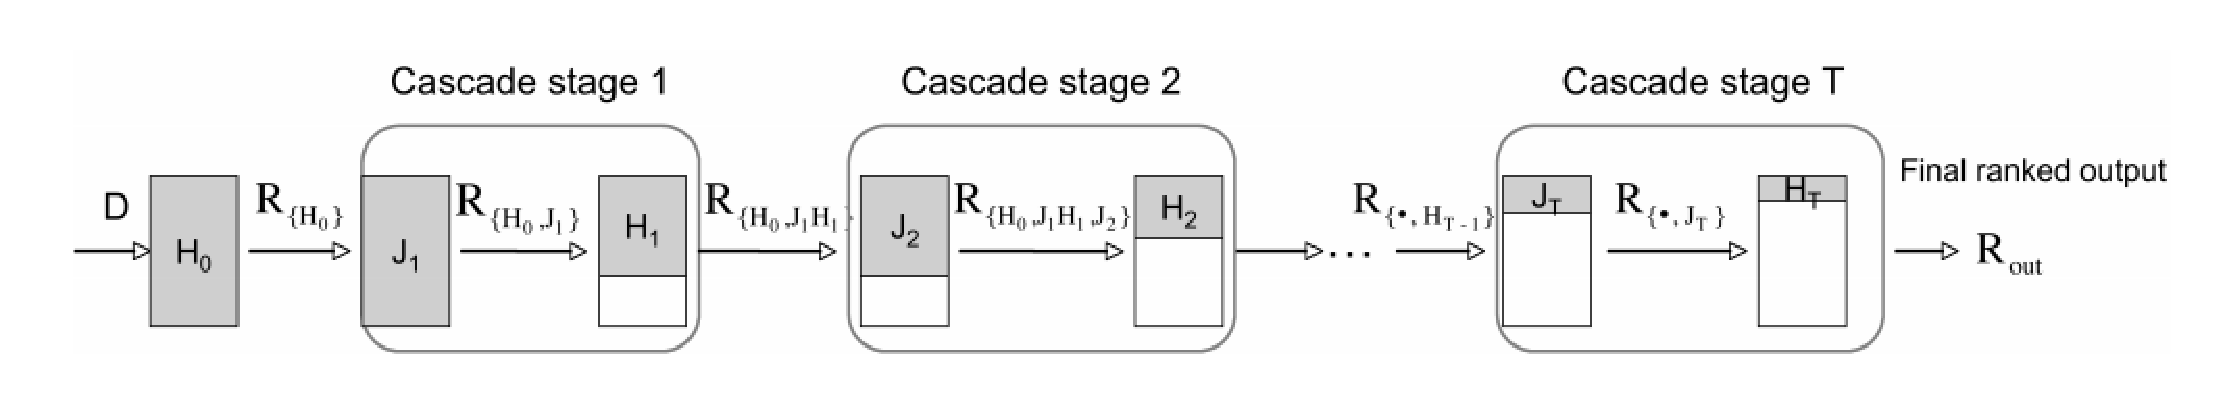
\includegraphics[width=0.9\textwidth]{figures/cascademodel.eps}
  \caption{级联模型}\label{fig:cascademodel}
\end{figure}

级联模型可以使用一组前后相继的阶段模型$\{\langle J_t(\beta_t), H_t, \alpha_t\rangle\}_{t=1}^T$来表示,每个阶段产生一个\textbf{完整的阶段模型},包括含参的剪枝模型$J_t(\beta_t)$、 弱排名函数$H_t$及其权值$\alpha_t$。为方便,记阶段$t$完整的阶段模型$S_t$:
\begin{equation}
    S_t = \langle J_t(\beta_t), H_t, \alpha_t\rangle
\end{equation}
在阶段$t$之前(包括阶段$t$)的所有阶段模型集合记为$G_t = \bigcup\limits_{i=0}^t S_i$。

\begin{algorithm}[htbp]
        \caption{级联排序算法}
        \begin{algorithmic}
            \REQUIRE ~~训练集$\{q_i,x_i,y_i\}^m_{i=1}$,级联阶数$T$,检索词概率分布$P_1(i)=1/m$,初始级联模型$G_0 =\varnothing$\\
            \FOR{$t = 1,\dots, T$}
            \STATE
            \begin{enumerate}
                \item 根据训练集检索词概率分布$P_t$,确定最佳的阶段模型$S_t = <J_t(\beta_t), H_t, \cdot>$:
                \begin{equation}
                    S_t = \argmin\limits_{S_t} \big[\eta_t^2 - \varphi_t^2\big]
                \end{equation}
                其中,%网格搜索(Grid Search)
                \begin{equation}
                    \left\{
                    \begin{array}{lll}
                      \eta_t & = & \sum\limits_{i=1}^m \frac{P_t(i)}{1-\gamma C(x_i,S_t)}\\
                      \varphi_t & = & \sum\limits_{i=1}^m \frac{P_t(i)}{1-\gamma C(x_i,S_t)} E(x_i,y_i,S_t)
                    \end{array}
                    \right.
                \end{equation}
                \item 给弱排名函数$H_t$赋最优权值$\alpha_t$:
                \begin{equation}
                    \alpha_t = \frac{1}{2} \log \frac{\eta_t + \varphi_t}{\eta_t - \varphi_t}
                \end{equation}
                \item 将完整的阶段模型$\langle J_t(\beta_t), H_t, \alpha_t\rangle$添加到$G_t$:
                \begin{equation}
                    G_t = G_{t-1} \cup \{\langle J_t(\beta_t), H_t, \alpha_t\rangle\}
                \end{equation}
                \item 根据级联模型在各个检索词上的表现,更新检索词的分布$P_{t+1}$:
                \begin{equation}
                    P_{t+1}(i)= \frac{\exp\{-E(x_i,y_i,f_t) + \gamma C(x_i,G_t)\}}{Z_t}
                \end{equation}
                其中,
                \begin{equation}
                    \left\{
                    \begin{array}{l}
                      f_t = \sum\limits_{k=1}^t \alpha_k H_k\\
                      E(x_i,y_i,f_t) = E(x_i,y_i,G_t)\\
                      Z_t = \sum\limits_{i=1}^{m} \exp\{-E(x_i,y_i,f_t) + \gamma C(x_i,G_t)\}
                    \end{array}
                    \right.
                \end{equation}
            \end{enumerate}
            \ENDFOR
            \ENSURE ~~最终排名函数$f_T = \sum\limits_{t=1}^{T}{\alpha_t H_t}$
        \end{algorithmic}
\end{algorithm}

级联排序问题属于多目标规划问题,为了兼顾模型效果与效率,级联模型定义了基于模型性能与计算开销的线性组合形式的\textbf{平衡度量指标(Tradeoff Metric)}:
\begin{equation}
    \mathrm{TM}_{ti} = E(x_i, y_i, G_t) - \gamma C(x_i, G_t)
\end{equation}
其中,$E(x_i,y_i,G_t)$表示直至阶段$t$的级联模型在检索词$q_i$上的排名效果,$C(x_i,G_t)$表示直至阶段$t$的级联模型的计算成本,$\gamma \in [0,1]$平衡两种指标对平衡度量指标的贡献,文中选择$\gamma = 0.1$。当$\gamma = 0$ 时,级联排序模型就简化成AdaRank模型,因此级联排序模型可以看做是AdaRank模型的推广。

成本函数$C(x_i, G_t)$一般可以使用下面的加和形式表示:
\begin{equation}
    C(x_i, G_t) = \sum\limits_{k=1}^t C(x_i, S_t)
\end{equation}
对于每个级联阶段,影响计算成本的因素包括排名模型$H_t$的复杂度,参与评估的文档数目,需要一种合适的成本估计方法。

通过对每个弱排名函数$H_t$(类似AdaRank,选择特征空间中的单个特征作为备选的弱排名函数)评估训练集中所有的检索词,并记录相应的时间开销,基于平均时间开销$U_t$ 估计计算成本:
\begin{equation}
    C(x_i, S_t) = U_t |R_{i\{\cdot, J_t\}}|
\end{equation}
其中,$|R_{i\{\cdot, J_t\}}|$表示参与评估的文档数目。为计算方便,作者选择衰减的指数函数$e^{-\delta C(x_i, G_t)}$,将计算成本映射到$[0,1]$区间,其中,$\delta  = 0.01$。

由此,可以定义下面形式的损失函数:
\begin{equation}
    \mathcal{L} = \frac{1}{m}\sum\limits_{i=1}^m \ell_i = \frac{1}{m} \sum\limits_{i=1}^m \exp \{ - E(x_i,y_i,G_t) + \gamma C(x_i,G_t)\})
\end{equation}

剪枝函数的作用是约减待评价的文档集,因为在实际应用中,多数文档属于不相关文档,那么预先将其从文档集中剔除,在提高文档整体质量的同时也提升了排名的效率。通常,剪枝函数都是含参$\beta_t$的评价准则,常用的剪枝函数有三种:
\begin{enumerate}
  \item 基于排名的剪枝函数(Rank-based):
  \[
    J_t(\beta_t) : \theta_t = (1-\beta_t) \times |R_{\{\cdot,H_{t-1}\}}|
  \]
  其中,$|R_{\{\cdot,H_{t-1}\}}|$表示在第$t$阶段输入的文档数目。这种剪枝函数要求对于排名低于$\theta_t$的文档剪枝。参数$\beta_t$越大,则剔除的文档越多(数值越小,名次越高)。
  \item 基于分值的剪枝函数(Score-based):
  \[
    J_t(\beta_t) : \theta_t = \beta_t \times [\max(R_{\{\cdot,H_{t-1}\}}) - \min(R_{\{\cdot,H_{t-1}\}})] + \min(R_{\{\cdot,H_{t-1}\}})
  \]
  其中,$max(R_{\{\cdot,H_{t-1}\}})$,$min(R_{\{\cdot,H_{t-1}\}})$表示$R_{\{\cdot,H_{t-1}\}}$中最大、最小的分值。如果文档的分值低于$\theta_t$,则从集合中剪除。
  \item 均值-最大值阈值准则(Mean-Max Threshold):
  \[
    J_t(\beta_t) : \theta_t = \beta_t \times \max(R_{\{\cdot,H_{t-1}\}}) + (1-\beta_t) \times \mathrm{mean}(R_{\{\cdot,H_{t-1}\}})
  \]
  其中,$\mathrm{mean}(R_{\{\cdot,H_{t-1}\}})$表示$R_{\{\cdot,H_{t-1}\}}$中文档的平均分值。如果待测文档分值低于$\theta_t$,则从集合中剪除。
\end{enumerate}

级联排序模型使用剪枝函数逐阶削减输入文档的数目,将相关性低的文档提前从输入集合中剔除,在提升训练效率的同时有助于改善文档集合的综合质量:
\begin{equation}
    \begin{array}{l}
      |R_{\{\cdot,J_t\}}| \le |R_{\{\cdot,J_{t-1}\}}| \le \cdots \le |R_{\{\cdot,J_1\}}|\\
      E(R_{\{\cdot,H_t\}}) \ge E(R_{\{\cdot,H_{t-1}\}}) \ge \cdots \ge E(R_{\{\cdot,H_0\}})
    \end{array}
\end{equation}
下面我们来证明级联排序模型具有持续改善排名性能的作用,证明步骤类似于AdaRank。

\begin{proof}
根据$\varphi_t, \eta_t, \alpha_t$的定义可知:
\begin{equation}
    e^{\alpha_t} = \sqrt{\frac{\eta_t + \varphi_t}{\eta_t - \varphi_t}}
\end{equation}

由于模型中用于衡量排序性能的指标$E\in [0,1]$,所以$e^{-E} \ge 1-E$,从而有:
\begin{equation}
    \begin{array}{lll}
      \frac{1}{m} \sum\limits_{i=1}^m \bigg[E(x_i, y_i, f_T) - \gamma C(x_i, G_T)\bigg] & \ge & \frac{1}{m} \sum\limits_{i=1}^m \bigg\{ 1 - exp\{-E(x_i, y_i, f_T) + \gamma C(x_i, G_T)\} \bigg\} \\
       & = & 1 - \frac{1}{m} \sum\limits_{i=1}^m exp\{-E(x_i, y_i, f_T) + \gamma C(x_i, G_T)\} \\
       & = & 1 - \frac{1}{m} Z_T
    \end{array}
\end{equation}
建立了模型平均性能指标同$Z_T$的关系,进而转向对$Z_T$上界的分析。

由于
\[
\begin{array}{lll}
      -E(x_i, y_i, f_T) + \gamma C(x_i, G_T) & = & \big[-E(x_i, y_i, f_T) + \alpha_T E(x_i, y_i, H_T) + E(x_i, y_i, f_{T-1})\big] \\
       & + & \big[- E(x_i, y_i, f_{T-1}) + \gamma C(x_i, G_{T-1}) \big]\\
       & + & \big[\gamma C(x_i, S_T) - \alpha_T E(x_i, y_i, H_T) \big]
\end{array}
\]
所以有:
\begin{equation}
    \begin{array}{lll}
      Z_T & = & \sum\limits_{i=1}^m exp\{-E(x_i, y_i, f_T) + \gamma C(x_i, G_T) \big]\} \\
       & = & \sum\limits_{i=1}^m \bigg[e^{-\delta_i^T} exp\{-E(x_i, y_i, f_{T-1}) + \gamma C(x_i, G_{T-1}\} exp\{\gamma C(x_i, S_T) - \alpha_T E(x_i, y_i, H_T)\} \bigg] \\
       & \le & e^{-\delta_{min}^T} Z_{T-1} \sum\limits_{i=1}^m \bigg[\frac{exp\{-E(x_i, y_i, f_{T-1}) + \gamma C(x_i, G_{T-1}\}}{Z_{T-1}} exp\{\gamma C(x_i, S_T) - \alpha_T E(x_i, y_i, H_T)\}\bigg] \\
       & = & e^{-\delta_{min}^T} Z_{T-1} \sum\limits_{i=1}^m P_T(i) exp\{\gamma C(x_i, S_T) - \alpha_T E(x_i, y_i, H_T)\} \\
       & \triangleq & e^{-\delta_{min}^T} Z_{T-1}  W_T
    \end{array}
\end{equation}
由于当$x>0$时,有$e^x \le \frac{1}{1-x}$,所以:
\begin{equation}
    e^{\gamma C(x_i, S_T)} \le \frac{1}{1 - \gamma C(x_i, S_T)}
\end{equation}
又因为:
\[
    -\alpha_T E(x_i, y_i, H_T) = \lambda (-\alpha_T) + (1-\lambda) \alpha_T
\]
其中,
\[
    \lambda = \frac{1+E(x_i,y_i,H_T)}{2}
\]
根据函数$f(x)=e^x$的凸性可知:
\begin{equation}
    e^{-\alpha_T E(x_i, y_i, H_T)} \le \frac{1+E(x_i,y_i,H_T)}{2} e^{-\alpha_T} + \frac{1-E(x_i,y_i,H_T)}{2} e^{\alpha_T}
\end{equation}

那么:
\begin{equation}
    \begin{array}{lll}
       W_T & = & \sum\limits_{i=1}^m P_T(i) exp\{\gamma C(x_i, S_T) -\alpha_T E(x_i, y_i, H_T)\} \\
       & \le & \sum\limits_{i=1}^m  \frac{P_T(i)}{1 - \gamma C(x_i, S_T)} e^{-\alpha_T E(x_i, y_i, H_T)} \\
       & \le & \sum\limits_{i=1}^m  \frac{P_T(i)}{1 - \gamma C(x_i, S_T)} \bigg\{\frac{1+E(x_i,y_i,H_T)}{2} e^{-\alpha_T} + \frac{1-E(x_i,y_i,H_T)}{2} e^{\alpha_T} \bigg\} \\
       & = & \sum\limits_{i=1}^m \frac{P_T(i)}{1 - \gamma C(x_i, S_T)} \bigg[ \frac{1+E(x_i,y_i,H_T)}{2}\bigg] e^{-\alpha_T} + \sum\limits_{i=1}^m \frac{P_T(i)}{1 - \gamma C(x_i, S_T)} \bigg[ \frac{1-E(x_i,y_i,H_T)}{2}\bigg] e^{\alpha_T}\\
       & = & \frac{\eta_T + \varphi_T}{2} e^{-\alpha_T} + \frac{\eta_T - \varphi_T}{2} e^{\alpha_T} \\
       & = & \sqrt{\eta_T^2 - \varphi_T^2}
    \end{array}
\end{equation}

从而可推知:
\begin{equation}
    \begin{array}{lll}
       Z_T & \le &  e^{-\delta_{min}^T} Z_{T-1} \sqrt{\eta_T^2 - \varphi_T^2}\\
       & = & Z_{T-2} \prod\limits_{t=T-1}^T e^{-\delta_{min}^t} \sqrt{\eta_t^2 - \varphi_t^2} \\
       & = & Z_1 \prod\limits_{t=2}^T e^{-\delta_{min}^t} \sqrt{\eta_t^2 - \varphi_t^2} \\
    \end{array}
\end{equation}

由于
\begin{equation}
    \begin{array}{lll}
      Z_1 & = & exp\{-E(x_i,y_i, \alpha_1 H_1) + \gamma C(x_i, G_1)\} \\
       & \le & e^{-\delta_{\min}^1} \sum\limits_{i=1}^m exp\{-\alpha_1 E(x_i,y_i, H_1) + \gamma C(x_i, S_1)\} \\
       & \le & e^{-\delta_{\min}^1} \sum\limits_{i=1}^m \frac{exp\{-\alpha_1 E(x_i,y_i, H_1)\}}{1-\gamma C(x_i, S_1)} \\
       & = & m \cdot e^{-\delta_{\min}^1} \big[e^{-\alpha_1} \sum\limits_{i=1}^m \frac{P_1(i)}{1-\gamma C(x_i, S_1)} \frac{1+E(x_i,y_i,H_1)}{2} + e^{\alpha_1} \sum\limits_{i=1}^m \frac{P_1(i)}{1-\gamma C(x_i, S_1)} \frac{1-E(x_i,y_i,H_1)}{2}\big]\\
       & = & m \cdot e^{-\delta_{\min}^1} \sqrt{\eta_1^2 - \varphi_1^2}
    \end{array}
\end{equation}

通过上面推导结果可知:
\begin{equation}
    Z_T \le m \prod\limits_{t=1}^T e^{-\delta_{\min}^t} \sqrt{\eta_t^2 - \varphi_t^2}
\end{equation}
因而可得:
\begin{equation}\label{eq:cascaderanktheorem}
    \frac{1}{m} \sum\limits_{i=1}^m \bigg[E(x_i, y_i, f_T) - \gamma C(x_i, G_T)\bigg] \ge 1- \prod\limits_{t=1}^T e^{-\delta_{\min}^T}  \sqrt{\eta_t^2 - \varphi_t^2},
\end{equation}
证毕。
\end{proof}

根据不等式\eqref{eq:cascaderanktheorem}可知,只要在每步迭代保证:
\[
    e^{-\delta_{\min}^t}  \sqrt{\eta_t^2 - \varphi_t^2} < 1
\]
成立,则排序模型的平均性能下界趋于上升,由此表明级联排名算法可以持续改善模型性能。

\section{排序逻辑回归模型}
2006年,Yan与Hauptmann~\cite{yan2006efficient}提出一种基于间隔(Margin-based)的广义排名学习框架,通过近似优化序对型风险函数估计模型参数,使用不同形式的损失函数与规则化项,可以推演出不同形式的排序模型,比如使用Logit 损失函数,他们提出了排序逻辑回归(Ranking Logistic Regression,RLR)模型,实验表明基于间隔的排序框架性能显著。

序对型排序学习方法将排名问题转化为二元分类问题,在分类框架下通过优化下面形式的正则化经验风险训练排序模型:
\begin{equation}
    \min\limits_{f} R_0(f) = \sum\limits_{q\in Q} \sum\limits_{i=1}^{n_q} L(y_i f(d_i,q)) + C\Omega(\|f\|_{\mathcal{H}})
\end{equation}
其中,第一部分是一般的经验风险,第二部分是正则化项。$Q$是检索词集合,$n_q$是同检索词$q$关联的文档数目,$y_i f(d_i,q)$是分类模型的“间隔”~\cite{hastie2009elements},$L$表示损失函数,一般地是关于间隔的递减函数,$\Omega$表示单调递增的规则化函数,$C>0$代表正则化系数。

分类框架下学习排序模型存在两个主要弊端,一方面模型预测精度对数据分布敏感,即某种类型的数据分布越多,则相应的预测结果就越倾向于此类型。另一方面,分类精度与排名精度不一致,模型分类精度很高,但是相应的排名性能未必尽如人意。为此,我们可以通过最大化同序对(Concordant Pairs)克服这些问题:
\begin{equation}
    \max\limits_f  \sum\limits_{q\in Q} \sum\limits_{d_i\in D_q^+} \sum\limits_{d_j\in D_q^-} I(f(d_i,q)>f(d_j,q))
\end{equation}

分析同序对可以发现,直接优化是行不通的,如果使用一个连续的、凸的、单调递减的损失函数替换它,势必可以方便模型优化工作。通过引入正则化项,本文给出下面统一形式的基于间隔的排序学习框架:
\begin{equation}
    \begin{array}{lll}
      \min\limits_{f} R_1(f) & = & \sum\limits_{q\in Q} \sum\limits_{d_i\in D_q^+} \sum\limits_{d_j\in D_q^-} L(f(d_i,q)-f(d_j,q)) + C\Omega(\|f\|_{\mathcal{H}}) \\
       & = & \sum\limits_{q\in Q} \sum\limits_{d_i\in D_q^+} \sum\limits_{d_j\in D_q^-} L(\sum\limits_{k=1}^n \omega_k[f_k(d_i,q) - f_k(d_j,q)]) + C\Omega(\|f\|_{\mathcal{H}})
    \end{array}
\end{equation}
排序模型选择最简单的线性模型$f(d,q) = \sum\limits_{k=1}^n \omega_k f_k(d,q)$,通过选择不同的损失函数与正则化项,就可以导出一系列排序模型。

\begin{definition}[排名一致性]
风险最小估计模型因子$\omega\in \mathbb{R}^n$,对任意的$d_i\in D_q^+,d_j\in D_q^-$,排名特征$f_k$如果满足$\omega_k(f_k(d_i,q) - f_k(d_j,q))\ge 0$,则称风险最小估计特征权值$\omega_k$与真实排名一致,我们称模型满足排名一致性(Rank Consistency)。
\end{definition}

\begin{theorem}
基于间隔的排序框架学习到的风险最小估计量$\omega_k$与真实排名一致。
\end{theorem}

\begin{proof}
如果存在排名特征$f_k$满足$f_k(d_i,q)\ge f_k(d_j,q),\forall q\in Q, d_i\in D_q^+,d_j\in D_q^-$,我们用反证法证明$\omega_k \ge 0$。 假设$\omega_k<0$,若记$\omega_k' = - \omega_k$,基于间隔的排序框架使用的损失函数是单调递减的,由于
\begin{equation}
    \omega_k (f_k(d_i,q) - f_k(d_j,q)) \le \omega_k'(f_k(d_i,q) - f_k(d_j,q))
\end{equation}
记$\Delta_k = \sum\limits_{l\ne k}  \omega_l(f_l(d_i,q) - f_l(d_j,q))$,则有
\begin{equation}
    L(\omega_k'(f_k(d_i,q) - f_k(d_j,q))+\Delta_k) \le L(\omega_k (f_k(d_i,q) - f_k(d_j,q)) + \Delta_k)
\end{equation}
这与$\omega_k$是风险最小估计量矛盾,故而$\omega_k\ge 0$。
\end{proof}

\begin{theorem}
若损失函数$L$是凸的,并且满足$2L(x/2)\ge L(x)$,则不等式成立:
\begin{equation}
    \frac{1}{2} \big[R_2(f) - R_2(-f)\big] \le R_1(f) \le R_2(f)
\end{equation}
其中,$R_1(f)$不含正则项,$R_2(f)$是一个基于有偏置的排名函数$f^b(d,q)$近似风险函数:
\begin{equation}
    R_2(f) = \sum\limits_{q\in Q} \bigg\{\sum\limits_{d_i\in D_q^+} |D_q^-| L(f^b(d_i,q)) + \sum\limits_{d_j\in D_q^-} |D_q^+| L(-f^b(d_j,q))\bigg\}
\end{equation}
其中,$|\cdot|$表示集合大小,$f^b(d,q) = \sum\limits_{k=1}^n \omega_k (f_k(d,q) - b_k)$。
\end{theorem}

\begin{proof}
由于损失函数是凸的并且$2L(x/2)\ge L(x)$,则对任意的$A,B\in \mathbb{R}$,都有
\[
    L(A) + L(B) \ge 2L(\frac{A+B}{2})\ge L(A+B)
\]
类似地可得
\[
    L(A+B) + L(-B) \ge 2L(\frac{A}{2})\ge L(A), L(A+B) + L(-A) \ge L(B)
\]
将两个不等式相加有:
\[
    2L(A+B) + L(-B) + L(-A) \ge L(A) + L(B)
\]
整理可得$L(A+B) \ge \frac{1}{2} \big[L(A) + L(B) - L(-A) - L(-B)\big]$,综上:
\begin{equation}
    L(A) + L(B) \ge L(A+B) \ge \frac{1}{2} \big[L(A) + L(B) - L(-A) - L(-B)\big]
\end{equation}

令$A=f^b(d_i,q),B=-f^b(d_j,q)$,我们有
\begin{equation}
    \begin{array}{lll}
      L(f^b(d_i,q)) + L(-f^b(d_j,q)) & \ge & L(f^b(d_i,q)-f^b(d_j,q)) = L(f(d_i,q)-f(d_j,q))\\
       & \ge & \frac{1}{2} \big[L(f^b(d_i,q)) + L(-f^b(d_j,q)) - L(-f^b(d_i,q)) - L(f^b(d_j,q))\big]
    \end{array}
\end{equation}
两边同时加和
\begin{equation}
    \begin{array}{ll}
       & \sum\limits_{q\in Q} \sum\limits_{d_i\in D_q^+} \sum\limits_{d_j\in D_q^-} \big[L(f^b(d_i,q)) + L(-f^b(d_j,q))\big]\\
       \ge & \sum\limits_{q\in Q} \sum\limits_{d_i\in D_q^+} \sum\limits_{d_j\in D_q^-} L(f(d_i,q)-f(d_j,q))\\
       \ge & \frac{1}{2} \sum\limits_{q\in Q} \sum\limits_{d_i\in D_q^+} \sum\limits_{d_j\in D_q^-} \big[L(f^b(d_i,q)) + L(-f^b(d_j,q)) - L(-f^b(d_i,q)) - L(f^b(d_j,q))\big]
    \end{array}
\end{equation}
由于第一个不等式
\begin{equation}
    \begin{array}{ll}
        & \sum\limits_{q\in Q} \sum\limits_{d_i\in D_q^+} \sum\limits_{d_j\in D_q^-} \big[L(f^b(d_i,q)) + L(-f^b(d_j,q))\big] \\
      = & \sum\limits_{q\in Q} \big\{\sum\limits_{d_i\in D_q^+}|D_q^-| L(f^b(d_i,q))+\sum\limits_{d_j\in D_q^-}|D_q^+|L(-f^b(d_j,q))\big\} \\
      = & R_2(f)
    \end{array}
\end{equation}
因此可得第二个不等式
\begin{equation}
    \begin{array}{ll}
        & \frac{1}{2} \sum\limits_{q\in Q} \sum\limits_{d_i\in D_q^+} \sum\limits_{d_j\in D_q^-} \big[L(f^b(d_i,q)) + L(-f^b(d_j,q)) - L(-f^b(d_i,q)) - L(f^b(d_j,q))\big] \\
      = & \frac{1}{2} \big[R_2(f) - R_2(-f)\big] \\
    \end{array}
\end{equation}
综上有$\frac{1}{2} \big[R_2(f) - R_2(-f)\big] \le R_1(f) \le R_2(f)$。特别地,如果$L$是线性的,则等式成立。
\end{proof}

近似风险函数$R_2(f)$的计算复杂度是$\complex(|D_q^+| + |D_q^-|)$远低于$R_1(f)$的复杂度$\complex(|D_q^+||D_q^-|)$,此外通过系数$|D_q^+|,|D_q^-|$ 抵消两类数据分布不平衡的影响,最大化两类数据的预测间隔。

如果取Logit损失函数
\begin{equation}
    L(x) = \log(1+e^{-x})
\end{equation}
那么有
\[
    L(x) + L(-x) = \log(1+e^{-x}) + \log(1+e^{x}) \le 2 + |x|
\]

在模型训练之前,必须首先确定偏置向量$b$,为此,可通过最小化上下界之差
\begin{equation}
    b^* = \argmin\limits_b \frac{1}{2} \big[ R_2(f) + R_2(-f)\big]
\end{equation}
使近似风险函数$R_2$更贴近于$R_1$的准确值,由于
\begin{equation}
    \frac{1}{2} \big[ R_2(f) + R_2(-f)\big] \le 2|Q||D_q^+||D_q^-| + \frac{1}{2} \sum\limits_{q\in Q} \bigg\{\sum\limits_{d_i\in D_q^+} |D_q^-| |f^b(d_i,q)|  + \sum\limits_{d_j\in D_q^-} |D_q^+| |f^b(d_j,q)|\bigg\}
\end{equation}
偏置向量的优化等价于下面的优化问题
\begin{equation}
    \min\limits_b \sum\limits_{q\in Q} \bigg\{\sum\limits_{d_i\in D_q^+} |D_q^-| |f^b(d_i,q)|  + \sum\limits_{d_j\in D_q^-} |D_q^+| |f^b(d_j,q)|\bigg\}
\end{equation}
直接优化难以实现,为此,使用一组优化模型逐个优选偏置量,达到近似优化的目的:
\begin{equation}
    \min\limits_{b_k} \sum\limits_{q\in Q}\bigg\{\sum\limits_{d_i\in D_q^+} |D_q^-| |f_k(d_i,q) - b_k|  + \sum\limits_{d_j\in D_q^-} |D_q^+| |f_k(d_j,q) - b_k|\bigg\}
\end{equation}
最优的偏置量是同一个排名特征下,所有检索词关联文档特征值的中值:
\begin{equation}
    \omega_k^* = \mathrm{median}\bigg\{\bigcup\limits_{q \in Q} \bigg(\bigcup\limits_{d_i \in D_q^+} \big\{f_k(d_i,q)\big\}_{|D_q^-|} \bigcup \bigcup\limits_{d_j \in D_q^-} \big\{f_k(d_j,q)\big\}_{|D_q^+|} \bigg)\bigg\}
\end{equation}
其中,$\{x\}_n$表示$n$个数值都等于$x$的集合,等价于将每个排名特征中值都转化为0。

将最优的偏置向量代入至$R_2(f)$中,使用Logit损失函数与$\ell_2$规则化项,我们可以利用梯度下降法进行优化。

\section{序对协调排名方法}
假设检索词$q$的关联文档集合是$\{x_i,r_i\}_{i=1}^n$,利用训练集学习线性模型$f(\omega,x)=\omega^T x$,我们要求模型在单个文档、文档序对及文档序列层面具有下面三条性质:
\begin{enumerate}
  \item 逐点型:预测结果与真实相关等级之间的误差尽可能小
  \[
    \argmin\limits_{\omega}~\sum\limits_{i=1}^n \|\omega^T x_i - r_i\|
  \]
  \item 序对型:对于检索词$q$的任意两个关联文档$x_i,x_j$,基于预测分值的排名结果与真实排名一致
  \[
    (\omega^T x_i - \omega^T x_j)(r_i - r_j) = \omega^T (x_i - x_j)(r_i - r_j) \ge 0
  \]
  \item 序列型:在检索词$q$上的排名精度尽可能高
  \[
    \argmax\limits_{\omega}~E(q,f)
  \]
  其中,$E$表示衡量排序性能的标准指标,如MAP、NDCG等。
\end{enumerate}

\textbf{序对型约束条件}要求预测模型能够最大化\textbf{序对间隔},由此建立下面形式的优化问题
\[
  \max\limits_{\omega} ~~\sum\limits_{(i,j)} \omega^T (x_i - x_j)(r_i - r_j)
\]
由于
\[
    (x_i - x_j)(r_i - r_j) = (x_j - x_i)(r_j - r_i)
\]
则原始问题等价于下面形式的优化问题
\begin{equation}\label{eq:clr}
  \max\limits_{\omega} ~~\sum\limits_{(i,j) \in \mathscr P} \omega^T (x_i - x_j)(r_i - r_j)
\end{equation}
其中,集合$\mathscr P$表示文档偏好序对集,定义为
\[
   \mathscr P = \{(i,j)\mid r_i > r_j, i,j = 1,\ldots, n\}
\]
对同序对间隔项进行整理,可得:
\begin{equation}\label{eq:concordantmargin}
 \begin{array}{ll}
    & \sum\limits_{(i,j) \in \mathscr P} (x_i - x_j)(r_i - r_j) \\
    = & \sum\limits_{(i,j) \in \mathscr P} \bigg[ x_i(r_i - r_j) - x_j(r_i - r_j)\bigg] \\
    = & \sum\limits_{i=1}^n x_i \sum\limits_{j\in \mathscr P_{i*}} (r_i - r_j) + \sum\limits_{j=1}^n x_i \sum\limits_{i\in \mathscr P_{*j}} (r_i - r_j) \\
    = & \sum\limits_{i=1}^n x_i \sum\limits_{j\in \mathscr P_{i*}\bigcup \mathscr P_{*i}} (r_i - r_j)\\
    \equiv & \sum\limits_{i=1}^n x_i \alpha_i
 \end{array}
\end{equation}
其中,集合
\[
    \mathscr P_{i*} = \{j\mid (i,j)\in \mathscr P, \forall j=1,\ldots,n\},~~\mathscr P_{*i} = \{j\mid (j,i)\in \mathscr P, \forall j=1,\ldots,n\}
\]
是根据样本$i$的相关等级对样本集合做出的一种,前者是所有等级低于$i$的样本集合,后者是所有等级高于$i$的样本集合。此外,还有一部分样本,它们的等级与样本$i$的相同,记为$\mathbb{S}_r$:
\begin{equation}
    \mathbb{S}_r = \{i\mid r_i = r, \forall i=1,\ldots,n\}, \forall r\in \mathbb{G}
\end{equation}
其中,样本$i$的相关等级等于$r$,$\mathbb{G}$表示数据集上所有相关等级的集合。

序对协调排名方法(Pairwise Concordant Ranking Method,PCRank)在优化问题\eqref{eq:clr}之上添加一个规则化项:
\begin{equation}
    L(\omega, \lambda) = \omega^T \sum\limits_{i=1}^n x_i \alpha_i - \frac{\lambda}{2} \| \omega \|^2
\end{equation}
若取$\ell_2-$范数,由极值必要性条件可知
\begin{equation}
    \omega^* = \frac{1}{\lambda} \sum\limits_{i=1}^n x_i \alpha_i
\end{equation}
其中,$\omega^*$是最优解,在不产生混淆的情况下,我们略去上标星号。由于$\lambda>0$,不会影响预测的排名结果,等价于
\begin{equation}
    \omega = \sum\limits_{i=1}^n x_i \alpha_i
\end{equation}
其中,$X\in\mathbb{R}^{n\times m}$表示训练数据集,每行表示一个数据样本特征向量。

我们利用等价关系
\[
    \mathscr P_{i*} \cup \mathscr P_{*i} = \{1,\ldots,n\}\backslash \mathbb{S}_r
\]
进一步化简等式\eqref{eq:concordantmargin},可得
\begin{equation}
 \begin{array}{lll}
    \omega & = & \sum\limits_{i=1}^n x_i \alpha_i \\
    & = & \sum\limits_{i=1}^n x_i \sum\limits_{j\in \mathscr P_{i*} \cup \mathscr P_{*i}} (r_i - r_j)\\
    & = & \sum\limits_{r\in \mathbb{G}} \sum\limits_{j\notin \mathbb{S}_r} (r - r_j) \sum\limits_{i\in \mathbb{S}_r} x_i\\
    & = & \sum\limits_{r\in \mathbb{G}} [(n - |\mathbb{S}_r|)r -\sum\limits_{j\notin \mathbb{S}_r} r_j] \sum\limits_{i\in \mathbb{S}_r} x_i\\
    & = & \sum\limits_{r\in \mathbb{G}} [nr - \sum\limits_{r_0\in \mathbb{G}} r_0|\mathbb{S}_{r_0}|] \sum\limits_{i\in \mathbb{S}_r} x_i \\
    & \equiv & \sum\limits_{r\in \mathbb{G}} (\beta_r \sum\limits_{i\in \mathbb{S}_r} x_i)
 \end{array}
\end{equation}
当$r$是最小的相关等级,则必然有$\beta_r\le 0$;反之,当$r$是最大的相关等级,则必然有$\beta_r>0$。如果训练数据只包含一种相关等级,则$\omega=0$。

若数据集线性不可分,引入核函数$K$则有:
\begin{equation}
    \begin{array}{lll}
      \omega^T \phi(x) & = & \sum\limits_{r\in \mathbb{G}} [nr - \sum\limits_{r_0\in \mathbb{G}} r_0|\mathbb{S}_{r_0}|] \sum\limits_{i\in \mathbb{S}_r} \phi(x_i)^T \phi(x) \\
      & = & \sum\limits_{r\in \mathbb{G}} [nr - \sum\limits_{r_0\in \mathbb{G}} r_0|\mathbb{S}_{r_0}|] \sum\limits_{i\in \mathbb{S}_r} K(x_i,x)
    \end{array}
\end{equation}
其中,$\phi$是映射函数,将输入变量映射到再生核Hilbert特征空间。\textcolor{blue}{基于核函数的PCRank存在一个严重的问题,在模型预测时所有的训练样本输入特征都要参与计算,无疑是不可行的。我们可以根据每个相关等级(或类别)下的输入特征,确定输入特征向量各个维度的区间范围,使用特征边界建立预测模型。}

利用相关等级可将关联文档集合划分成多个等价类,统计各个等价类下样本个数$|\mathbb{S}_{r_0}|$,只需复杂度为$\complex(n)$的时间就可以迅速确定对应与检索词$q$的最佳线性模型。我们使用此办法,对不同检索词构建不同的线性模型,作为基本排名函数,使用AdaRank算法,基于Boosting技术集成为强排名函数。

在确定最佳基本线性模型时,模型参数(特征权值)可能存在负值,并且对各个等级相关文档分布十分敏感。对于同一组数据集,相关等级经过保序变换,本质上并不会影响预测模型的排名精度。本模型可能会受到相关等级保序变换的影响,我们下面考察保序变换对线性模型的影响(假设相关等级保序变换函数为$\psi$):
\begin{equation}
    \begin{array}{lll}
      \beta_r \sum\limits_{i\in \mathbb{S}_r} x_i & = & nr - \sum\limits_{r_0\in \mathbb{G}} r_0|\mathbb{S}_{r_0}| \sum\limits_{i\in \mathbb{S}_r} x_i\\
      & = & \sum\limits_{r_0\in \mathbb{G}} |\mathbb{S}_{r_0}| (r-r_0) \sum\limits_{i\in \mathbb{S}_r} x_i\\
      & = & \sum\limits_{r_0\in \mathbb{G}} |\mathbb{S}_r| |\mathbb{S}_{r_0}| (r-r_0) \sum\limits_{i\in \mathbb{S}_r} x_i/ |\mathbb{S}_r|\\
      & = & \bar{x}_r \sum\limits_{r_0\in \mathbb{G}} |\mathbb{S}_r| |\mathbb{S}_{r_0}| (r-r_0)
    \end{array}
\end{equation}
因此,$\beta$可以看做是每个相关等级所有文档特征向量加权平均值权重。

相关等级进行线性变换$\psi(r) = a*r+b$
\begin{equation}
    \beta_r' \sum\limits_{i\in \mathbb{S}_r} x_i = \bar{x}_r \sum\limits_{r_0\in \mathbb{G}} |\mathbb{S}_r| |\mathbb{S}_{r_0}| [\psi(r) - \psi(r_0)] = a \beta_r \sum\limits_{i\in \mathbb{S}_r} x_i
\end{equation}
对关联文档的排名不会产生任何影响。

在PCRank模型中,相同等级的文档序对Pairwise Concordance间隔无任何贡献。分析模型的预测精度可以发现,相同等级的文档预测结果越接近则模型预测精度越高
\begin{equation}
    \min\limits_{\omega} ~\sum\limits_{r\in \mathbb{G}} \sum\limits_{i,j\in \mathbb{S}_r} |\omega^T x_i - \omega^T x_j|
\end{equation}
并且对于等级越高的文档序对,它们的预测接近程度更有利于提升模型整体的预测精度,为此可以添加权重因子
\begin{equation}
    \max\limits_{\omega} ~\sum\limits_{r\in \mathbb{G}} \sum\limits_{i,j\in \mathbb{S}_r} \varphi(r) |\omega^T x_i - \omega^T x_j|
\end{equation}
由于在文档标记中,相关等级数值越小则等级越高,则$\varphi(r)$是关于相关等级的单调递减函数,比如$\varphi(r)=e^{-r}$。

将相同等级的文档序对预测结果接近程度添加到PCRank模型中,建立下面形式的模型(统一称为PCRank模型)
\begin{equation}
    \max\limits_{\omega} ~ \sum\limits_{(i,j)\in \mathscr P} (\omega^T x_i - \omega^T x_j) [\psi(r_i)-\psi(r_j)] - \gamma \sum\limits_{r\in \mathbb{G}} \sum\limits_{i, j\in \mathbb{S}_r} \varphi(r) |\omega^T x_i - \omega^T x_j| - \frac{1}{2} \lambda \|\omega\|^2
\end{equation}
其中,$\lambda>0$,函数$\psi$是关于相关等级$r$的单调递增函数,提升模型在高相关等级文档上的预测精度,$\gamma>0$可以融入到单调递减函数$\varphi$ 中。

\textcolor{blue}{
假设预测函数为$f$,一般性的PCRank模型可以表示如下
\begin{equation}
    \max\limits_{f\in \mathcal H} ~ J(\theta,\lambda) = \sum\limits_{(i,j)\in \mathscr P} \big[f(x_i) - f(x_j)\big] [\psi(r_i)-\psi(r_j)] - \sum\limits_{r\in \mathbb G} \sum\limits_{i, j\in \mathbb{S}_r} \varphi(r) \big|f(x_i) - f(x_j)\big| - \frac{1}{2} \lambda \|f\|_\mathcal{H}^2
\end{equation}
}
模型反映了聚类的部分思想:使不同类别的样本数据尽量分散,相同类别的样本数据尽量聚集,并保证预测结果与真实相关等级的一致性。PCRank模型可以应用到多元分类问题

PCRank模型可以应用到分类问题:选择最优的阈值$b$(每个分类一个阈值),确保分类误差最小:
\begin{equation}
    \argmax\limits_{b} ~\sum\limits_{r\in \mathbb{G}} \sum\limits_{i\in \mathbb{S}_r} I(g(\omega^T x_i + b_r) = y_i)
\end{equation}

\section{公开数据集:排序学习}
排序学习是典型的监督学习方法,使用包含人工标记的数据作为训练数据集训练模型。目前,支持排序学习训练、检测的数据集很多,比如微软亚洲研究院提供的LETOR\cite{qin2010letor}、Microsoft Learning to Rank、Yahoo! Learning to Rank Challenge、Yandex Internet Mathematics等。

\subsection{LETOR}
目前,LETOR
\footnote{LETOR: \href{http://research.microsoft.com/en-us/um/beijing/projects/letor/}{http://research.microsoft.com/}}
公开数据集是排序学习研究人员使用最多的标准数据集,并且还提供多种经典排序学习算法的实验结果。LETOR是\textbf{LE}arning \textbf{TO} \textbf{R}ank的缩写,由微软亚洲研究院(Microsoft Research Asia,MSRA)发布。从2007年4月至2009年7月,MSRA已经发布了四个版本,本文实验使用的数据集是LETOR 3.0与LETOR 4.0两个版本。本节主要介绍实验中使用的LETOR数据集基本信息。

LETOR数据集包含的数据信息有三个主要部分:检索词集合、文档集合(也称“语料库”)、文档与检索词的相关等级。检索词集合与文档集合来源不同,前者统一标记赋予唯一的ID号,后者源自于网络采集程序从互联网上抓取的网页数据,并且以数值型的文档特征向量形式存储。文档与检索词的相关等级是监督学习的“标准答案”,部分来自于人工标记,还有是根据Bing搜索引擎的搜索日志生成。在LETOR 3.0数据包中含有七个数据集:HP2003、HP2004、NP2003、NP2004、TD2003、TD2004 和OHSUMED,LETOR 4.0 则含有两个数据集:MQ2007与MQ2008。

LETOR 3.0使用的文档集合是OHSUMED和Gov语料库。OHSUMED语料库\cite{hersh1994ohsumed}属于医学文献数据库MEDLINE的一个数据集,由1987年至1991年刊发的、出自270 个医学期刊的348,566篇医学文献构成。OHSUMED数据集由106个检索词,大约16,140篇文档构成,每篇文档提取45个特征,并根据文档与检索词的相关程度标记为三个等级:高度相关、部分相关、不相关。Gov语料库包含大约1,053,110篇网页,是2002年初从域名后缀为.gov的政府网站上爬取下来的。2003年,Gov语料库开始用于文本检索会议(Text REtrieval Conference,TREC)Web检索项目\cite{craswell2003overview}下的主题提取(Topic Distillation,TD)、主页发现(Home Page Finding,HP)和命名网页发现(Named Page Finding,NP)三类检索任务,语料库中每篇网页提取64个特征,文档与检索词的相关性标记为两个等级:相关与不相关。2003年、2004年文本检索会议Web 检索项目使用的数据集有六组:TD2003,TD2004,HP2003,HP2004,NP2003,NP2004。LETOR 4.0使用的文档集合是Gov2语料库、使用的检索词集合源自2007 年、2008 年文本检索会议Million Query(MQ)项目,分别记为MQ2007与MQ2008。Gov2语料库源自2004年初从政府网站上爬取下来的25,000,000篇网页,达到426G。语料库中每篇网页提取46个特征。MQ2007、MQ2008分别包含1700条、800条检索词。每个检索词文档,所有训练数据标记为三个等级:高度相关、相关、不相关。

\subsection{Microsoft Learning to Rank}
数据集采自Bing的标签集合,相关等级有5个级别:0(不相关)$\sim$ 4(完全相关)。它包含两组数据集:MSLR-WEB30k、MSLR-WEB10k,前者包含30,000个检索词,后者只有10,000检索词。每对query-doc包含136个特征。

\subsection{Yahoo! Learning to Rank Challenge}
Yahoo! 实验室于2010年初举办了一次Learning to Rank 挑战赛
\footnote{\href{http://webscope.sandbox.yahoo.com/catalog.php?datatype=c}{Yahoo! Learning to Rank Challenge}}
,使用的数据源自Yahoo!自己用作训练排名函数的子数据集。它包含两组数据集,一大一小,分别被分割成三个子数据集:训练集、验证集、测试集。数据包含700个特征,评价分5个等级:0(不相关)$\sim$ 4(高度相关)。\cite{chapelle2011yahoo}总结了竞赛的结果,并对胜出模型做出评价。

\subsection{Yandex Internet Mathematics}
Yandex是俄罗斯目前最大的搜索引擎公司,于2009年组织了一场互联网数学竞赛(Internet Mathematics Challenge)
\footnote{Internet Mathematics Challenge: \href{http://imat2009.yandex.ru/en}{2009}, \href{http://imat-relpred.yandex.ru/en}{2011}}
,竞赛使用的数据分成两部分:训练集与测试集。训练集中包含9,124条检索词,97,290篇文档。测试集总共包含115,643篇文档,取出21,103篇文档作为公开测试数据,其他用作最终测试。每篇文档提取245个特征,训练数据由人工标记为5个等级(0$\sim$4)。


\section{排序学习算法汇总表}
\begin{table}[ht]
\centering
    \begin{tabular}{|l|l|l|l|l|l|l|}
      \hline
      类型 & 名称 & 时间 & 损失函数 & 优化方法 & 数据集 & 对比算法\\
      \hline
      SVM & RankSVM\cite{joachims2002optimizing} &2002 & & & &\\
      SVM & IR-SVM\cite{cao2006adapting} & 2006& & & &\\
      SVM & SVM\textsuperscript{MAP}\cite{yue2007support} &2007 & & & &\\
      \hline
      ANN & PRank\cite{crammer2001pranking} & 2001 & & & &\\
      ANN & RankNet\cite{burges2005learning} & 2005 & & & &\\
      ANN & LambdaRank\cite{burges2007learning} & 2007 & & & &\\
      ANN & LambdaMART\cite{burges2010from} & 2010 & & & &\\
      ANN & ListNet\cite{cao2007learning} & 2007 & & & &\\
      ANN & ListMLE\cite{xia2008listwise} & 2008 & & & &\\
      ANN & QBRank\cite{zheng2007general}& 2007 & & & &\\
      ANN & FRank\cite{tsai2007frank}& 2007 & & & &\\
      ANN & SortRank\cite{rigutini2008sortnet}& 2008 & & & &\\
      ANN & BoltzRank\cite{volkovs2009boltzrank}& 2009 & & & &\\
      \hline
      Boosting & RankBoost\cite{freund2003efficient} & 2003& & & &\\
      Boosting & AdaRank\cite{xu2007adarank} & 2007& & & &\\
      Boosting & RankCosine\cite{qin2008query} & 2008& & & &\\
      Boosting & SRankBoost\cite{amini2008boosting} & 2008 & & & &\\
      Boosting & NDCGBoost\cite{valizadegan2009learning} & & & & &\\
      Boosting & GBRank\cite{zheng2007regression} & 2007 & & & &\\
      Boosting & RankRefine\cite{jin2008ranking} & & & & &\\
      Boosting & MPBoost\cite{zhu2009general} & & & & &\\
      Boosting & GBlend\cite{chen2010learning}& 2010 & & & &\\
      \hline
      Regression & SLR\cite{cooper1992probabilistic} & 1992 & & & &\\
      Regression & RankLR\cite{sculley2009large} & 2009 & & & &\\
      Regression & CRR\cite{sculley2010combined} & 2010 & Combined & SGD & &\\
      Regression & IntervalRank\cite{moon2010intervalrank} & 2010 & & & &\\
      -- & RankGP\cite{yeh2007learning} & 2007 & & GA & &\\
      -- & McRank\cite{li2007mcrank} & 2007 & & & &\\
      -- & SoftRank\cite{taylor2008softrank} & 2008 & & &\\
      -- & RankRLS\cite{pahikkala2009efficient}  & 2009 & & & &\\
      Bayes & BayesRank\cite{kuo2009learning}  & 2009 & & & &\\
      -- & PermuRank\cite{xu2008directly} & 2008& & & &\\
      \hline
    \end{tabular}
\end{table}
%--------------learning to rank
\chapter{度量指标}
在机器学习、数据挖掘、推荐算法等学术实验分析阶段,通常要经过一个模型性能评价的过程。
%模型评价依赖于两方面因素:评价指标与公开数据集。
本章主要介绍在各个领域常用的评价或度量指标。
%公开数据集、数据采样技术、数据标准化和交叉检验。

\ornamento

%度量空间(Metric Space)和测度(Measure Theory in Probability)
\section{度量空间与测度论}
\section{范数}
\subsection{H\"{o}lder范数}
对于无约束范数逼近问题:
\begin{equation}\label{eq:normmin}
    \min~\|Ax - b\|_p
\end{equation}
其中,$A\in \mathbb{R}^{m\times n}, b\in \mathbb{R}^m$,$p>0$。

如果$p\ge 2$,则范数是$\ell_p$范数或称H\"{o}lder范数:
\begin{equation}
    f(x) \triangleq \|Ax - b\|_p = \Big[\sum\limits_i |a_i^T x - b_i|^p\Big]^\frac{1}{p}.
\end{equation}

我们定义
\[
    g(x) \triangleq f(x)^p = \|Ax - b\|_p^p = \sum\limits_i |a_i^T x - b_i|^p
\]
由于$g(x)$二阶处处可微,根据Newton法,可以得到下面的迭代序列:
\begin{equation}
    \begin{array}{lll}
      x_{k+1} & = & x_k -\alpha_k (\nabla^2 g(x_k))^{-1} \nabla g(x_k) \\
       & = & x_k - \frac{\alpha_k}{p-1} (A^T W_k A)^{-1} A^T W_k (A x_k - b) \\
       & = & \frac{p - 1 - \alpha_k}{p-1} x_k + \frac{\alpha_k}{p-1} (A^T W_k A)^{-1} A^T W_k b \\
       & = & \frac{p - 1 - \alpha_k}{p-1} x_k + \frac{\alpha_k}{p-1} \argmin\limits_{\bar{\omega}} \|W_k^{1/2}(A \bar{\omega} - b)\|_2
    \end{array}
\end{equation}
其中,$x_0 = 0$,$\alpha_k\in [0,1)$是固定的,或者根据线性搜索技术迭代变化。$W_k$是个对角矩阵:
\begin{equation}
    W_k \triangleq
    \begin{pmatrix}
        (a_1^T x_k - b_1)^{p-2} & 0 & \cdots & 0 \\
        0 & (a_2^T x_k - b_2)^{p-2} & \cdots & 0 \\
        \vdots & \vdots & \ddots & \vdots \\
        0 & 0 & 0 & (a_m^T x_k - b_m)^{p-2}
    \end{pmatrix}
\end{equation}

\subsection{曼哈顿范数}
当$p=1$时,问题\eqref{eq:normmin}转化为最小化$\ell_1$或曼哈顿范数(Manhattan Norm):
\[
    f(x) \triangleq \|Ax - b\|_1 = \sum\limits_i |a_i^T x - b_i|
\]
我们可以藉由下面的线性规划问题进行求解:
\[
    \begin{array}{ll}
      \textit{min} & \sum\limits_i \nu_i \\
      \textit{s.t.} & |a_i^T x - b_i|\le \nu_i, i = 1,\ldots,m \\
    \end{array}
\]

在机器学习任务中,常涉及到稀疏模型的训练问题,通过优化$\ell_1$正则项的非平滑损失函数学习模型,比如回归分析中的Lasso算法。

\subsection{欧式范数}
当$p=2$时,问题\eqref{eq:normmin}就是$\ell_2$或者欧式范数(Euclidean Norm)的最小化:
\[
    f(x) \triangleq \|Ax - b\|_2 = \sqrt{\sum\limits_i (a_i^T x - b_i)^2}
\]
是典型的最小二乘问题,存在下面等价的二次规划形式:
\[
    \min~f(x)^2 = \|Ax - b\|_2^2 = \sum\limits_i (a_i^T x - b_i)^2
\]
存在解析解(Analytic Solution, Closed Form Solution)
\[
    \hat x = (A^T A)^{-1}A^T b
\]

\subsection{切比雪夫范数}
当$p = \infty$时,问题\eqref{eq:normmin}转化为最小化$\ell_{\infty}$或者切比雪夫范数(Chebyshev Norm,也称“棋盘距离”):
\[
    f(x) \triangleq \|Ax - b\|_{\infty} = \max\limits_i |a_i^T x - b_i|
\]
由于不存在解析解,我们可以将其转化为下面的线性规划问题:
\[
    \begin{array}{ll}
      \textit{min} & \nu \\
      \textit{s.t.} & |a_i^T x - b_i|\le \nu, i = 1,\ldots,m \\
    \end{array}
\]

\subsection{L最大范数}
向量$\omega\in \mathbb{R}^m$的\textbf{L最大范数(Largest-L Norm)}$\|\omega\|_{[L]}$是将$\omega$按照其坐标绝对值降序排列,前$L$个最大坐标绝对值之和,即有定义
\begin{equation}\label{eq:largestlnorm}
    \|\omega\|_{[L]} = \sum\limits_{i=1}^L |\omega|_{[i]}, ~~~1\le L\le m,
\end{equation}
其中,$|\omega|_{[i]}$表示坐标绝对值降序排列第$i$位的数值,满足$|\omega|_{[1]} \ge |\omega|_{[2]} \ge \ldots \ge |\omega|_{[m]}$。
当$L=1$时,L最大范数等价于$\ell_{\infty}$范数;当$L=m$时,等价于$\ell_1$范数;当$1 < L < m$时,它是一个凸函数,最小化L最大范数等价于解线性规划问题
\begin{equation}\label{eq:minlargestlnorm}
    \begin{array}{ll}
      \textit{min} & \sum\limits_i c_i + Lq \\
      \textit{s.t.} & |a_i^T x - b_i|\le c_i + q,\\
      & c_i \ge 0, ~~~1\le i\le m.
    \end{array}
\end{equation}
多数人在面对最小化L最大范数问题时,会选择复杂的障碍函数法(Barrier Method)或次梯度法(Subgradient Method),纵然是优化问题专业人员亦鲜有人知可使用模型\eqref{eq:minlargestlnorm}简化问题。

\section{距离和相似性度量}
距离度量衡量对象间的差异程度,距离越远则对象间的差异越大。相似度度量衡量对象间的相似程度,与距离度量相反,相似度度量值越小,则说明对象间相似度越小,差异越大。其他相似性度量、距离度量可以参考\cite{cha2007comprehensive,lenz2008proximities}。

\subsection{闵可夫斯基距离}
闵可夫斯基距离(Minkowski Distance)是对多个距离度量公式的概括性的表述,公式如下:
\begin{equation}\label{eq:minkowski}
    d(x,y)=\Big[\sum\limits_i (x_i-y_i)^p\Big]^\frac{1}{p}
\end{equation}

\begin{enumerate}
  \item 当$p=1$时,闵可夫斯基距离退化成曼哈顿距离(Manhattan Distance):
      \begin{equation}\label{eq:manhattan}
        d(x,y) = \sum_i |x_i-y_i|
      \end{equation}
  它来源于城市区块距离,对多个维度上的距离求和。假设在曼哈顿街区乘坐出租车从一个地方到另一个地方,白色区域表示高楼大厦,灰色表示街道,三条折线都表示两地间的曼哈顿距离,三者长度相等。
  \begin{figure}[htbp]
    \centering
    \includegraphics[width=0.5\textwidth, height=6cm]{figures/ManhattanBlock.eps}\\
    \caption{曼哈顿街区与曼哈顿距离}\label{fig:manhattanblock}
  \end{figure}
  \item 当$p=2$时,闵可夫斯基距离退化成欧几里得距离(Euclidean Distance):
      \begin{equation}\label{eq:euclidean}
        d(x,y)=\sqrt {\sum\limits_i (x_i-y_i)^2}
      \end{equation}
  它是最常见的距离度量,衡量的是多维空间中点与点之间的绝对距离。如图~\ref{fig:manhattanblock}所示,中间绿色斜线表示两地之间的欧几里得距离。
  \item 当$p\rightarrow \infty$时,闵可夫斯基距离退化为切比雪夫距离(Chebyshev Distance):
      \begin{equation}\label{eq:chebyshev}
        d(x,y)=\lim_{p \rightarrow \infty}\Big[\sum\limits_i (x_i-y_i)^p\Big]^{1/p}=\max_{i} |x_i-y_i|
      \end{equation}
  它起源于国际象棋规则下国王的走法。
\end{enumerate}
  \begin{figure}[htbp]
    \centering
    \includegraphics[width=0.9\textwidth, height=1cm]{figures/UnitMinkowskiDist.eps}\\
    \caption{参数$p$与单位闵科夫斯基距离之间的关系图}\label{fig:unitminkowski}
  \end{figure}

\subsection{Cayley距离}
Cayley距离是度量有序变量无序性的指标。假设标准队列为$a$,$b$中至少有一个位置与$a$不同,通过交换$b$中的元素的位置可以将其变成标准队列(简称标准交换),Cayley距离对应最小的标准交换次数。如图\ref{fig:cayleydist},第一个队列是标准队列,我们可以最少交换三次第二个队列的位置对就可以变成标准队列,因此二者的Cayley距离为3。

\subsection{Ulam距离}
Ulam距离与Cayley距离类似,针对队列$b$,它可以使用删除-移动-插入的连环动作变成标准队列(简称标准变换)。Ulam距离对应最小的标准变换次数。如图
\ref{fig:ulamdist},第一个队列是标准队列,我们可以最少交换三次第二个队列的位置对就可以变成标准队列,因此二者的Ulam距离为2。

\begin{figure}[htbp]
    \begin{minipage}[t]{0.49\linewidth}
        \centering
          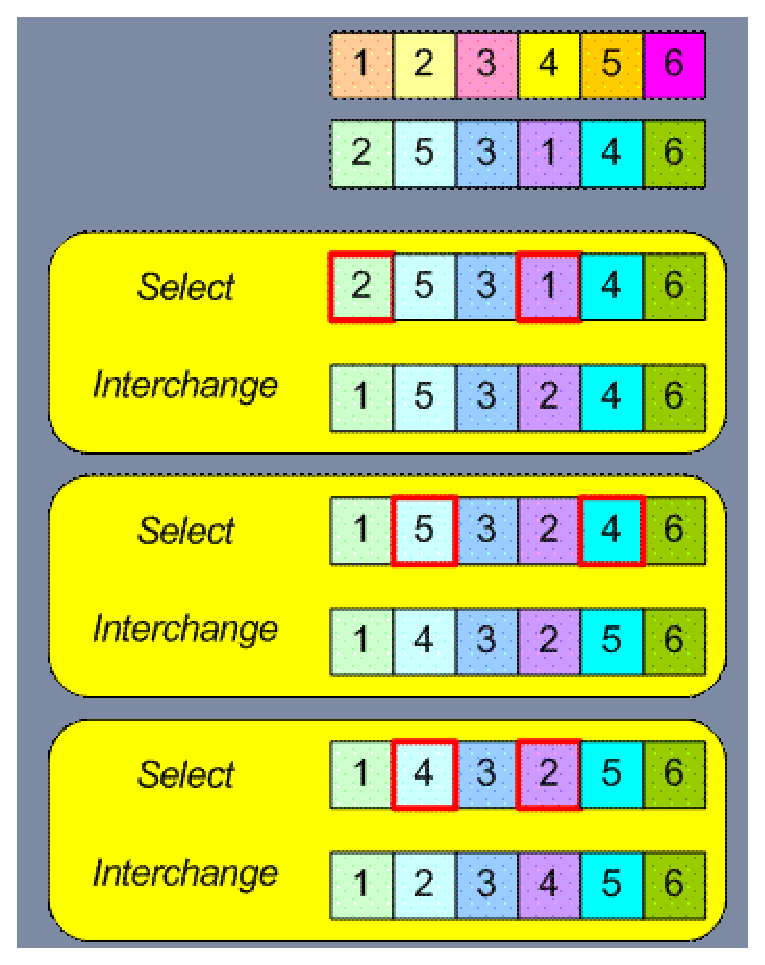
\includegraphics[width=0.95\textwidth,height=8cm]{figures/cayleydist}
          \caption{Cayley距离距离演示}\label{fig:cayleydist}
    \end{minipage}
    \begin{minipage}[t]{0.49\linewidth}
        \centering
          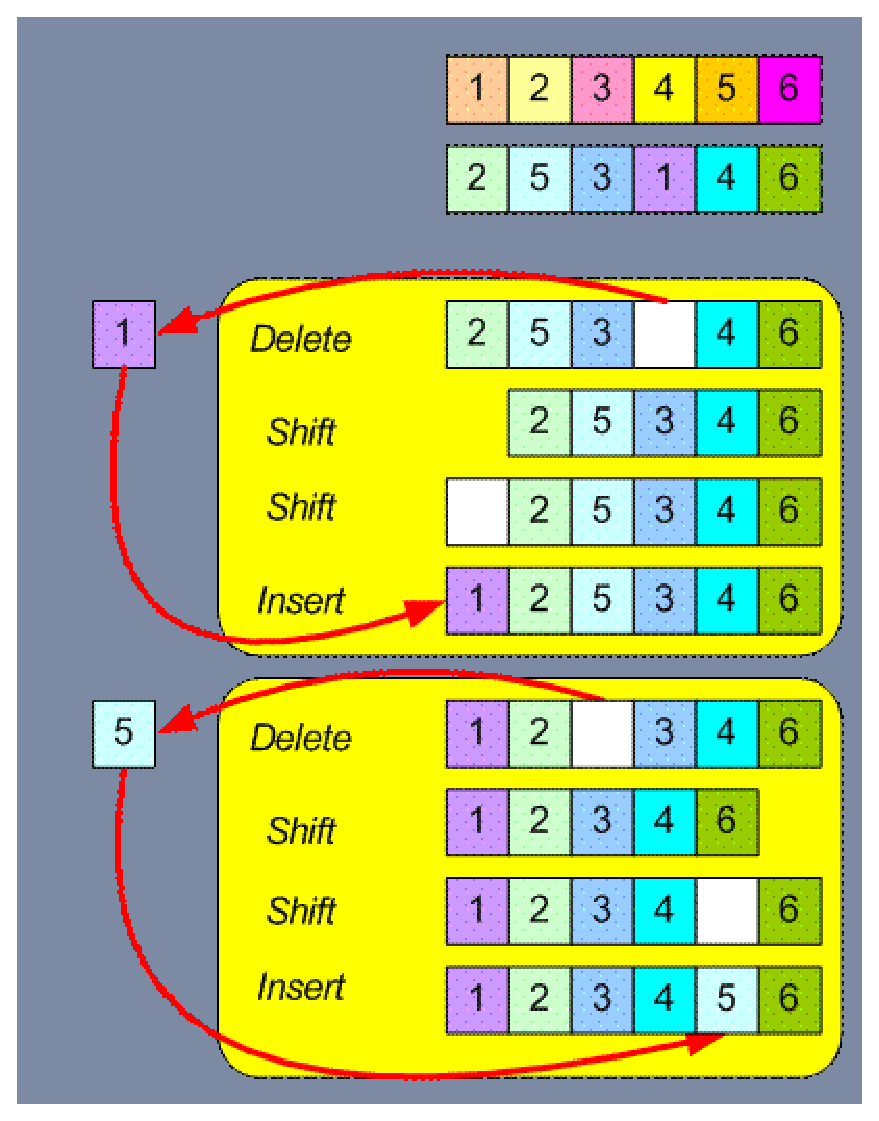
\includegraphics[width=0.95\textwidth,height=8cm]{figures/ulamdist}
          \caption{Ulam距离计算演示}\label{fig:ulamdist}
    \end{minipage}
\end{figure}

\subsection{汉明距离}
1950年,Richard Hamming~\cite{hamming1950error}引入了汉明距离(Hamming distance),亦称“信号距离”,用于度量两个等长字串相应位置字符不同的位置数目。汉明 距离还可以表示将一个字串变成另外一个字串需要替换的最小数目。对于两个二元字串$a,b$,它们的汉明距离即$a$ \textit{XOR} $b$中1的数目。

\subsection{月球漫步者距离}
它由Gaspard Monge在1781年首次提出,用以度量两个统计分布的差异。在数学上又称Wasserstein度量。

\subsection{余弦相似度}
向量空间两个向量夹角余弦值常用于衡量对象间的差异,具体定义如下:
\begin{equation}\label{eq:cosinesim}
    \cos\langle x,y\rangle=\frac{x^T y}{\|x\|\|y\|},
\end{equation}
余弦值越大,则两对象之间的差异越小;反之,则越大。余弦值可以直接用于度量对象之间的相似程度,此时称作\textbf{余弦相似度}(cosine similarity)。

\subsection{杰卡德系数}
对于两个集合$A$和$B$,如果我们只关心两者具有相同特征的比例,则可以使用如下形式的杰卡德系数(Jaccard coefficient)
\begin{equation}\label{eq:jaccard}
    J(A,B)=\frac{|A\cap B|}{|A\cup B|}
\end{equation}
度量对象间的相似程度。系数值越大,表明两个对象的相似性越强,反之则越弱。

\subsection{核相似度}
在实际应用中,我们可以直接将定义在向量空间上的核函数作为相似性度量,从而可以得到核相似性度量(kernel similarity)。比如高斯核函数定义的高斯相似性度量:
\begin{equation}\label{eq:kernelsim}
    K(x,y)=\exp\{-\frac{\|x-y\|^2}{2\sigma^2}\}.
\end{equation}

\subsection{皮尔逊相关系数}
皮尔逊相关系数(Pearson correlation coefficient)描述了两个变量间的线性相关性。对于变量$x$和$y$,假设均值分别是$\mu_x,\mu_y$,标准差分别是$\sigma_x,\sigma_y$,则总体相关系数定义如下:
\begin{equation}\label{eq:pearsoncor}
    \rho(x,y)=\frac{\cov(x,y)}{\sigma_x\sigma_y}=\frac{E\big[(x-\mu_x)(y-\mu_y)\big]}{\sigma_x\sigma_y}.
\end{equation}
基于$n$组样本对协方差和标准差的估计,我们可以使用下式计算样本相关系数:
\begin{equation}\label{eq:pearsonrho}
    \rho(x,y)=\frac{\sum\limits_i (x_i - \bar x)(y_i - \bar y)}{\sqrt{\sum\limits_i (x_i - \bar x)^2 \sum\limits_i (y_i - \bar y)^2}} = \frac{n\sum\limits_i (x_i y_i) - \sum\limits_i x_i \sum\limits_i y_i}{\sqrt{n\sum\limits_i x_i^2 - (\sum\limits_i x_i)^2}\sqrt{n\sum\limits_i y_i^2 - (\sum\limits_i y_i)^2}}.
\end{equation}
根据定义,皮尔逊相关系数$-1 \le \rho(x,y) \le 1$,通过$|\rho(x,y)|$的大小可以判定相关程度,$|\rho(x,y)|$越大,$x$和$y$的相关程度越大。当$\rho(x,y)=1$ 时,表示$x$和$y$完全正相关;当$\rho(x,y)=-1$表示完全负相关;当$\rho(x,y)=0$表示不相关。如果我们令$u_i=x_i-\bar x$,$v_i=y_i-\bar y$,$i=1,2,\ldots,n$,则皮尔逊相关系数实际上与夹角余弦相似度等价:
\begin{equation}
    \rho(u,v) = \frac{\sum\limits_i (x_i - \bar x)(y_i - \bar y)}{\sqrt{\sum\limits_i (x_i - \bar x)^2 \sum\limits_i (y_i - \bar y)^2}} = \cos\langle u,v\rangle.
\end{equation}

\subsection{等级相关系数}\label{subsec:spearman-and-kendall}
检索系统在执行检索时,对于同一个检索语句,不同搜索引擎由于内部排名算法的差异,可能检索到不完全相同的数据、产生截然不同的网页排名列表。等级相关系数
(rank correlation coefficient)是度量排名列表间相似性和相关性一类重要的统计量,常见的等级相关系数有:斯皮尔曼等级相关系数Footrule和Rho、肯德尔等级相关系数Tau、Goodman--Kruskal等级相关系数Gamma。研究人员已经将其应用到排名聚合、搜索效果评估问题,具有重要的实际意义。

假设$\pi$和$\sigma$是某个可排列对象单元集上的两个排名列表,可能表示评价主体根据对象单元的两个基本属性进行有序排列。比如例子\ref{eg:gallup-2016}中可排列对象单元对应五位民主党总统候选人$\big\{$Clinton,Warren,Cuomo,O'Malley,Biden$\big\}$,各自包含四个属性:公众熟识比例(Familiar)、公众认同的比例、公众排斥的比例和公众净认同比例。我们按照第一个属性对五人进行有序排列会产生一个排名列表(比如$\pi$),按照第四个属性排列他们又可以得到一个排名列表(比如$\sigma$)。为了度量排名列表$\pi$ 和$\sigma$之间的相似性,我们定义如下一般形式的等级相关系数:
\begin{equation}\label{eq:rankcoor}
    \gamma(\pi, \sigma) = \frac{\sum\limits_{i,j} g(\pi_i,\pi_j)h(\sigma_i,\sigma_j)}{\sqrt{\sum\limits_{i,j} g(\pi_i,\pi_j)^2 \sum\limits_{i,j} h(\sigma_i,\sigma_j)^2}},
\end{equation}
其中函数$g(\cdot)$和$h(\cdot)$各自依据排名列表$\pi$和$\sigma$ 评价所有可能的对象单元序对。比如,$g(\pi_i,\pi_j)$根据排名列表$\pi$评价对象单元序对$(i,j)$,$h(\sigma_i,\sigma_j)$则根据排名列表$\sigma$评价对象单元序对$(i,j)$。当函数$g(\cdot)$和$h(\cdot)$的形式如下:
\[
    g(\pi_i,\pi_j)  = \pi_i - \pi_j, ~~~ h(\sigma_i,\sigma_j)  = \sigma_i - \sigma_j,
\]
对应的等级相关系数就是等级相关系数Rho。如果函数$g(\cdot)$和$h(\cdot)$的形式如下:
\[
    g(\pi_i,\pi_j)  =  \sgn(\pi_i - \pi_j),~~~ h(\sigma_i,\sigma_j)  =  \sgn(\sigma_i - \sigma_j),
\]
对应的等级相关系数就是等级相关系数Tau。函数$g(\cdot)$ 和$h(\cdot)$对对象单元序对使用不同的评价标准,就会产生一种对应的等级相关性度量。此外,当我们把所有可能的对象单元序对逐一展开,函数$g(\cdot)$和$h(\cdot)$对它们的评价就形成两个高维的评价向量$V_g\in \mathbb R^{n^2}$和$V_h\in \mathbb R^{n^2}$:
\begin{eqnarray}
  V_g = (g_{11}, g_{12}, g_{21}, g_{13}, g_{31}, \ldots, g_{nn})^T, & g_{ij} \triangleq g(\pi_i,\pi_j),\\
  V_h = (h_{11}, h_{12}, h_{21}, h_{13}, h_{31}, \ldots, h_{nn})^T, & h_{ij} \triangleq h(\sigma_i,\sigma_j).
\end{eqnarray}
利用它们改写一般形式的等级相关系数\eqref{eq:rankcoor}:
\begin{equation}
    \gamma(\pi, \sigma) = \frac{V_g^T V_h}{\|V_g\|\|V_h\|} = \cos \langle V_g, V_h \rangle \in [-1, 1],
\end{equation}
本质上等于两个评价向量$V_g$和$V_h$的夹角余弦相似度。

\subsubsection{Spearman's Footrule与Rho}
1904年,实验心理学先驱、英国退伍军官查尔斯·斯皮尔曼Charles Spearman~\cite{spearman1904proof}延伸相关系数的概念,推导出等级相关的计算方法,提出Footrule度量,基于此开创出因子分析(factor analysis)方法~\cite{spearman1904general},成为其学术生涯最伟大的成就。

假设某对象集合存在两个排名列表$\pi$和$\sigma$,斯皮尔曼将Footrule定义为两列表差值的$\ell_1$范数:
\begin{equation}\label{eq:spearmanfootrule}
    \mathcal F(\pi,\sigma) = \sum\limits_i |\pi_i - \sigma_i|.
\end{equation}

斯皮尔曼等级相关系数Rho统计量则建立在所有对象单元序对之上,具体形式如下:
\begin{equation}
    \rho(\pi,\sigma) = \frac{\sum\limits_{i,j} (\pi_i - \pi_j)(\sigma_i - \sigma_j)}{\sum\limits_{i,j} (\pi_i - \pi_j)^2},
\end{equation}
其中$\pi_i$,$\sigma_i$分别表示排名对象集合第$i$个对象在排名列表$\pi$与$\sigma$上的名次。对于一个长度等于$n$的排名列表,存在$n(n-1)$个排名指标序对,并且满足
\[
    \sum\limits_{i,j} (\pi_i - \pi_j)^2 = \sum\limits_{i,j} (\sigma_i - \sigma_j)^2.
\]
我们可以根据如下两个事实
\begin{eqnarray}
  \sum\limits_i \pi_i = &1 + 2 + \cdots + n = n(n+1)/2 &= \sum\limits_i \sigma_i,\\
  \sum\limits_i \pi_i^2 = & 1^2 + 2^2 + \cdots + n^2 = n(n+1)(2n+1)/6 &=\sum\limits_i \sigma_i^2,
\end{eqnarray}
简化Rho统计量得:
\begin{equation}\label{eq:spearmanrho}
    \rho(\pi,\sigma) = 1 - \frac{6}{n^3-n} \sum\limits_i (\pi_i - \sigma_i)^2.
\end{equation}

\subsubsection{Kendall's Tau}
1938年,莫里斯·肯德尔Maurice Kendall\cite{kendall1938new}根据两个排名列表中排名对象的排名顺序是否一致,定义Tau统计量。一般地,Tau值越大,说明列表的差异越大。由于使用冒泡排序方法,将一个列表按照另一个列表的顺序排列需要移动的次数,恰好等于Tau值,Tau统计量由此又称作“冒泡排序距离”。

肯德尔定义的等级相关系数Tau是建立在一系列有序对的二元判断之上,表示如下:
\begin{equation}
    \tau(\pi,\sigma) = \frac{\sum\limits_{i,j} \sgn(\pi_i - \pi_j) \sgn(\sigma_i - \sigma_j)}{\sqrt{\sum\limits_{i,j} [\sgn(\pi_i - \pi_j)]^2 \sum\limits_{i,j} [\sgn(\sigma_i - \sigma_j)]^2}}.
\end{equation}
它是一个对称的统计量。当$i=j$时,和因子$\sgn(\pi_i - \pi_j)\sgn(\sigma_i - \sigma_j)= 0$。
在不考虑具体和因子的情况下,我们利用排名序对集$\mathscr P$化简Tau统计量的双重加和项
\[
    \sum\limits_{i,j} (\cdot) = \sum\limits_{i=1}^n \sum\limits_{j=1}^n (\cdot) = 2 \sum\limits_{i=1}^{n-1} \sum\limits_{j = i + 1}^n (\cdot)
    = 2 \sum\limits_{(i,j)\in \mathscr P}(\cdot),
\]
其中$\mathscr P = \big\{(i,j)|1\le i < j \le n\big\}$是由所有可能的序对构成的\textbf{序对集},容量$|\mathscr P|$ = n(n-1)/2。我们可以利用它简化Tau统计量的分子部分:
\[
    \sum\limits_{i,j} \sgn(\pi_i - \pi_j) \sgn(\sigma_i - \sigma_j)
     = 2\sum\limits_{(i,j)\in \mathscr P} \sgn\big[(\pi_i - \pi_j)(\sigma_i - \sigma_j)\big]
     \triangleq 2(|\mathscr P_{\pi,\sigma}^c| - |\mathscr P_{\pi,\sigma}^n|),
\]
其中$\mathscr P_{\pi,\sigma}^n$与$\mathscr P_{\pi,\sigma}^c$称作排列$\pi$和$\sigma$上的\textbf{(异)同序对集}((non-)concordant pairs)
\begin{eqnarray}
      \mathscr P_{\pi,\sigma}^c & = & \big\{(i,j)\in \mathscr P~|~\sgn[(\pi_i - \pi_j)(\sigma_i - \sigma_j)] = 1\big\}\subset \mathscr P, \\
      \mathscr P_{\pi,\sigma}^n & = & \big\{(i,j)\in \mathscr P~|~\sgn[(\pi_i - \pi_j)(\sigma_i - \sigma_j)] = -1\big\}\subset \mathscr P.
\end{eqnarray}
它们是$\mathscr P$上两个不相交的子集,其他部分称作$\pi$和$\sigma$上的\textbf{平局序对集}(tied pairs):
\begin{eqnarray}
    \mathscr P_{\pi,\sigma}^t  & = &  \big\{(i,j)\in \mathscr P~|~\sgn[(\pi_i - \pi_j)(\sigma_i - \sigma_j)] = 0\big\}\subset \mathscr P,
\end{eqnarray}
并且满足$|\mathscr P_{\pi,\sigma}^c| + |\mathscr P_{\pi,\sigma}^n| + |\mathscr P_{\pi,\sigma}^t| = |\mathscr P|$。此外,$\sgn[(\pi_i - \pi_j)(\sigma_i - \sigma_j)] = 0$对应三种可能局面:
\begin{eqnarray}
  |\sigma_i - \sigma_j| > 0, & \pi_i = \pi_j, \label{eq:tie-1}\\
  |\pi_i - \pi_j| > 0,& \sigma_i = \sigma_j, \label{eq:tie-2}\\
  \pi_i = \pi_j,& \sigma_i = \sigma_j, \label{eq:tie-3}
\end{eqnarray}
统计量的分母部分成分远比比分子部分复杂。为了方便细化分析,我们根据平局产生的排名列表将$\mathscr P_{\pi,\sigma}^t$分割成两个子集:
\begin{eqnarray}
  \mathscr P^t_\pi &=& \big\{(i,j)\in \mathscr P~|~\pi_i = \pi_j\big\}\subset \mathscr P_{\pi,\sigma}^t, \\
  \mathscr P^t_\sigma &=& \big\{(i,j)\in \mathscr P~|~\sigma_i = \sigma_j\big\}\subset \mathscr P_{\pi,\sigma}^t.
\end{eqnarray}
其中$\mathscr P_\pi^t$和$\mathscr P_\sigma^t$分别是排名列表$\pi$和$\sigma$上的平局序对集。

\textbf{(甲)}如果三种局面都没有出现,则集合$\mathscr P_\pi^t$和$\mathscr P_\sigma^t$都是空集,此时
\[
    \sum\limits_{i,j} [\sgn(\pi_i - \pi_j)]^2 = \sum\limits_{i,j} [\sgn(\sigma_i - \sigma_j)]^2 = n(n-1)
\]
那么Tau统计量就可以化简如下:
\begin{equation}\label{eq:kendalltau-notie}
    \tau(\pi,\sigma) = \frac{2(|\mathscr P_{\pi,\sigma}^c| - |\mathscr P_{\pi,\sigma}^n|)}{n(n-1)} = \frac{|\mathscr P_{\pi,\sigma}^c|}{|\mathscr P|} - \frac{|\mathscr P_{\pi,\sigma}^n|}{|\mathscr P|},
\end{equation}
等于同序对比例和异序对比例的差值,前一项表示两排名列表$\pi$和$\sigma$之间的相似度,后一项则表示两者的距离或相异程度,两项差值则衡量两排名列表间的相关程度(或净相似度),Tau值越高相关度就越高。

\textbf{(乙)}如果\eqref{eq:tie-1}\eqref{eq:tie-2}\eqref{eq:tie-3}三种局面至少出现一种,都需要对分母部分做相应调整:
\begin{eqnarray}
  \sum\limits_{i,j} [\sgn(\pi_i - \pi_j)]^2 = 2 \sum\limits_{(i,j)\in \mathscr P} [\sgn(\pi_i - \pi_j)]^2 = 2 \big(|\mathscr P| - |\mathscr P^t_\pi|\big), \\
  \sum\limits_{i,j} [\sgn(\sigma_i - \sigma_j)]^2 = 2 \sum\limits_{(i,j)\in \mathscr P} [\sgn(\sigma_i - \sigma_j)]^2 = 2 \big(|\mathscr P| - |\mathscr P^t_\sigma|\big).
\end{eqnarray}

Tau统计量可作如下简化:
\begin{equation}\label{eq:kendalltau-tie}
    \tau(\pi,\sigma) = \frac{|\mathscr P_{\pi,\sigma}^c| - |\mathscr P_{\pi,\sigma}^n|}{\sqrt{\big(|\mathscr P| - |\mathscr P^t_\pi|\big)\big(|\mathscr P| - |\mathscr P^t_\sigma|\big)}}.
\end{equation}
当$\pi$与$\sigma$上都没有平局序对时,\eqref{eq:kendalltau-tie}和\eqref{eq:kendalltau-notie}完全等价。如果$\pi=\sigma$,则$|\mathscr P_{\pi,\sigma}^c| = |\mathscr P|$,Tau统计量值最大$\tau(\pi,\sigma)=1$。如果$\pi$和$\sigma$彼此完全向逆,则$|\mathscr P_{\pi,\sigma}^n| = |\mathscr P|$,Tau统计量值最小$\tau(\pi,\sigma)=-1$。其他情况下,$-1 < \tau(\pi,\sigma) < 1$。

对于排名聚合问题,人们比较关心位于前列的对象的质量,然而Footrule和Tau均没有考虑位置信息对排名效果的影响。为此,有研究人员
\cite{kumar2010generalized,farnoud2012novel}提出两种统计量位置加权形式的扩展模型,使其满足如下两个基本特点:
\begin{enumerate}
  \item 假设在理想列表中,A、Z两个排名对象分别排在前列和后列,那么排名算法改变A的次序比改变Z的次序对整体排名质量的影响更大。
  \item 当排名算法的排名结果与理想排名结果完全一致时,二者距离最小;若排名结果完全相悖,则距离最大。
\end{enumerate}

\subsection{对数似然比}
对数似然比(log-likelihood ratio,LLR)~\cite{dunning1993accurate,wang2008multiple}是子参数空间与全参数空间的最大似然估计之比~\cite{dunning1993accurate},可用于度量对象之间的相似关系,比如统计用户$U$和$V$ 的在线购物历史记录,可构造如\ref{tbl:llr}所示的表格。
表格中$n_{11}$表示两个用户都喜欢的商品数目,$n_{22}$表示两个都不喜欢的商品数目,$n_{12}$表示用户$U$喜欢而用户$V$不喜欢的数目,$n_{21}$则完全相反。
\begin{table}[htbp]
    \centering
    \begin{tabular}{c|c|c}
      \hline
       & $V+$ & $V-$ \\
      \hline
      $U+$ & $n_{11}$ & $n_{12}$ \\
      \hline
      $U-$ & $n_{21}$ & $n_{22}$ \\
      \hline
    \end{tabular}
    \caption{用户购物的偏好统计矩阵}
    \label{tbl:llr}
\end{table}

对数似然比的计算需要一种信息熵,它定义如下:
\begin{equation}\label{eq:llr}
    \lambda = 2 \times (H_m - H_r - H_c)
\end{equation}
其中,$H_m = H(n_{11}, n_{12}, n_{21}, n_{22})$称作矩阵熵,$H_r = H(n_{11}, n_{12}) + H(n_{21}, n_{22})$为行熵,$H_c = H(n_{11}, n_{21}) + H(n_{12}, n_{22})$为列熵。这里信息熵定义如下:
\begin{equation}
    H(X) = -\sum\limits_i x_i \log \frac{x_i + z_i}{\sum\limits_i x_i}
\end{equation}
其中,$Z=(z_1, z_2, \ldots, z_n)$是统计变量$X$对应元素的反示性函数,如果$x_i=0$,则$z_i=1$,否则$z_i=0$。

\section{局部敏感哈希}
局部敏感哈希(Locality-Sensitive Hashing,LSH)是应用于海量高维数据上的一类近似最近邻(Approximate Nearest Neighbor)快速查找方法,广泛应用于网页查重、图像检索、音频检索、数据降维、聚类分析、推荐算法等场景。

\subsection{SimHash}
\subsection{MinHash}
%an algorithm used to detect duplicated documents, Andrei Z. Broder


\section{推荐系统评价指标}
衡量推荐系统的评价指标包括:均方根误差(Root Mean Squared Error,RMSE)、平均绝对误差(Mean Absolute Error,MAE)\cite{jensen2003reducing}、精度(Precision)、召回率(Recall)和DCG(Discount Cumulative Gain)。 在真实的推荐场景中,我们还希望推荐的内容具有新颖性(Novelty)和多样性(Diversity)。

推荐精度是评价推荐算法最基本的指标,它衡量的是推荐算法在多大程度上能够准确预测用户对推荐商品的喜欢程度。目前大部分的关于推荐系统评价指标的研究都是针对推荐精度的。精度指标有很多,有些衡量用户对商品的预测评分与真实评分的接近程度,有些只考虑推荐排名\cite{zhu2012recmetric}。

\subsection{均方根误差}
目前评价推荐精度的度量指标中,均方根误差(Root Mean Squared Error,RMSE)是使用最多的一种,也在多次推荐算法比赛中使用作为标准的度量指标。它的数学定义为:
\begin{equation}\label{eq:rmse}
    \text{RMSE} = \sqrt{\frac{1}{N}\sum\limits_k (p_k - q_k)^2},
\end{equation}
其中,$N$是测试数据集的大小,$P=(p_1,\ldots, p_N)^T$是待评分项真实评分值,$Q=(q_1,\ldots, q_N)^T$是模型预测分值。均方根误差越小,则说明模型预测评分与真实评分越一致,预测精度越高。

\subsection{平均绝对误差}
平均绝对误差(Mean Absolute Error,MAE)是推荐系统中最容易解释的一种度量指标,其数学定义如下:
\begin{equation}\label{eq:mae}
    \text{MAE} = \frac{1}{N} \sum\limits_k |p_k - q_k|.
\end{equation}

\subsection{多样性}
在推荐系统中,多样性体现在两个层次,用户间的多样性(Inter-user Diversity)和用户内的多样性(Intra-user Diversity)。前者反映推荐系统对不同用户推荐不同商品的能力,后者则反映推荐系统对一个用户推荐商品多种商品的能力。对于用户$u$和$v$,我们可以使用汉明距离(Hamming Distance)度量两个用户推荐列表$\mathcal I_u$与$\mathcal I_v$的差异程度,具体定义为:
\begin{equation}\label{eq:inter-diversity}
    d_{uv} = 1 - \frac{1}{L} |\mathcal I_u \cap \mathcal I_v|,
\end{equation}
其中$L$表示推荐列表的长度,也就是推荐的商品数目。系统中所有的用户对汉明距离的平均值反映了推荐系统的多样性水平,汉明距离越大,则多样性越强。用户$u$的商品推荐多样性依赖于推荐列表中商品相似性状况,定义如下:
\begin{equation}\label{eq:intra-diversity}
    d_u = \frac{1}{|\mathcal I_u|(|\mathcal I_u|-1)} \sum\limits_{\substack{i\ne j\\i,j \in \mathcal I_u}} s_{ij},
\end{equation}
系统中所有用户的用户内多样性均值反映了系统的多样性。

\subsection{A/B测试}
推荐系统的评价可分为在线评价和离线评价两种方式。在线评价其实就是设计在线用户实验,根据用户在线实时反馈或事后问卷调查等结果来衡量推荐系统的表现。

目前最常用的在线测试方法$A/B$测试。所谓$A/B$测试,简单而言就是为一个目标制定两套方案,相应地将用户也分割成两部分,一部分使用方案$A$,一部分使用方案$B$,并记录下用户的使用状况,选择出更符号设计目的的方案正式上线。$A/B$测试的基本准则是多方案并行测试、每个方案只有一个变量不同(单变量)、以某种规则优胜劣汰。$A/B$测试并非只同时测试两个方案,它可能会设计和测试多个方案,以确定各个方案的优劣\cite{zhu2012recmetric}。

\section{排名性能评价指标}
在信息检索领域,用于衡量排名性能的指标有多种,比如NDCG\cite{jarvelin2000ir,jarvelin2002cumulated},MAP\cite{baeza1999modern},MRR\cite{voorhees1999trec}等。本节简要介绍常见的几种性能度量指标。

\subsection{查准率}
在信息检索领域,精度(Precision,又称“查准率”)和召回率(Recall,又称“查全率”)是两个最常使用的,用以衡量检索性能的指标。精度是指检索到的文档中相关文档比率:
\begin{equation}\label{eq:precision}
    \text{P} = \frac{|A\cap B|}{|B|}
\end{equation}
其中,$A$表示系统中相关文档集合,$B$表示检索到的文档集合。

在排名问题中,精度主要用于度量两个级别的排名性能。在训练数据集中,每个排名文档包含一个相关等级,如果是相关的则记为1,否则记为0,那么排名列表$\pi$ 的第$k$个位置上的精度记为P@k,定义如下:
\begin{equation}\label{eq:precisionk}
    \text{P@k}=\frac{1}{k} \sum_{i=1}^{k}{I(y_{\pi^{-1}(i)}=1)}
\end{equation}
其中,$I(\cdot)$为示性函数。

\subsection{召回率}
召回率是指检索系统中返回的相关文档占所有相关文档的比例,可以表示成如下形式:
\begin{equation}\label{eq:recall}
    \text R = \frac{|A\cap B|}{|A|}
\end{equation}

实际上,“在海量的实时动态网络系统中,根本不可能估计系统中同检索词相关的文档数目”\cite{chu1996search},那么召回率就无法计算。
\cite{chu1996search,gwizdka1999towards}在研究搜索引擎的性能时均以此为由,将召回率从度量指标中剔除。将召回率直接剔除并不恰当,TREC Web Track使用样本池方法(Pooling Method)从系统中寻找相关文档,并假设没有落在池子中的样本是不相关的\cite{voorhees2001overview}。

对于二元分类问题,我们可以将真实的类别标记与模型预测结果的所有可能组合绘制到图\ref{fig:labelandpredict}。
\begin{figure}[htbp]
  \centering
  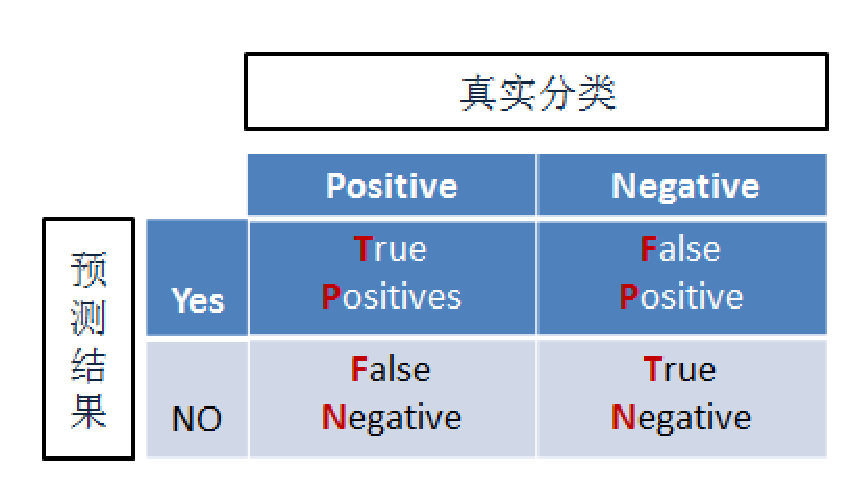
\includegraphics[width=0.5\textwidth, height = 5cm]{figures/labelandpredict.eps}
  \caption{真实标记与预测结果}\label{fig:labelandpredict}
\end{figure}
图\ref{fig:labelandpredict}构成一个分类器可信度的混淆矩阵(Confusion Matrix),以医学诊断\footnote{一般来说,阳性表示疾病或体内生理的变化有一定的结果,
阴性则基本上否定或排除某种病变的可能性}为例,其中的阳性(Positive)是“有病”,阴性(Negative)是“无病”,则False Positve是“假阳性”,将实际“无病
(Negative)”的人诊断为“有病(True)”,也称“误诊率”,属于“第I类错误”。False Negative是“假阴性”,将实际“有病(Positive)”的人诊断为“无病(False)”,也称“漏诊率”,属于“第II类错误”。统计学家认为犯第I类错误的代价高于犯第II类错误,实际上在不同的治疗阶段,两类错误的代价是不同的。

根据Precision与Recall的定义,结合图\ref{fig:labelandpredict},我们有:
\begin{equation}
  \begin{array}{l}
    \text{P} = \frac{\text{TP}}{\text{TP + FP}} \\
    \text{R} = \frac{\text{TP}}{\text{TP + FN}}
  \end{array}
\end{equation}

另外,根据预测与真实分类之间的一致性,还可以定义准确率(Accurate)、真阳性比率(True Positive Rate,TPR)、假阳性比率(False Positive Rate,FPR):
\begin{equation}
  \begin{array}{rcl}
    \text{Accurate} &=& \frac{\text{TP + TN}}{\text{TP + FP + TN + FN}} \\
    \text{TPR} &=& \frac{\text{TP}}{\text{TP + FN}} \\
    \text{FPR} &=& \frac{\text{FP}}{\text{FP + TN}} = 1 - \frac{\text{TN}}{\text{FP + TN}}
  \end{array}
\end{equation}

在20世纪50年代,英国Cranfield大学首先提出一套信息检索评价系统(简称Cranfield评价体系),由查询样本集、正确结果集和评价指标构成,并由此确立了“评价”在信息检索研究中的重要地位。Cranfield评价体系使用的两个评价指标是查准率和查全率,反映了标准检索系统的具备的两个基本能力:过滤不相关文档的能力,检索到所有相关文档的能力。查准率与查全率实际上是相互制约的,一般而言,查准率越高,则查全率下降,反之亦反。以查全率作为横轴,以查准率作为纵轴,二者的互斥关系可以使用Precison-Recall曲线(简称PR-Curve)\cite{davis2006relationship}描述,见图\ref{fig:prcurve}。

\begin{figure}[ht]
    \begin{minipage}[t]{0.49\linewidth}
        \centering
        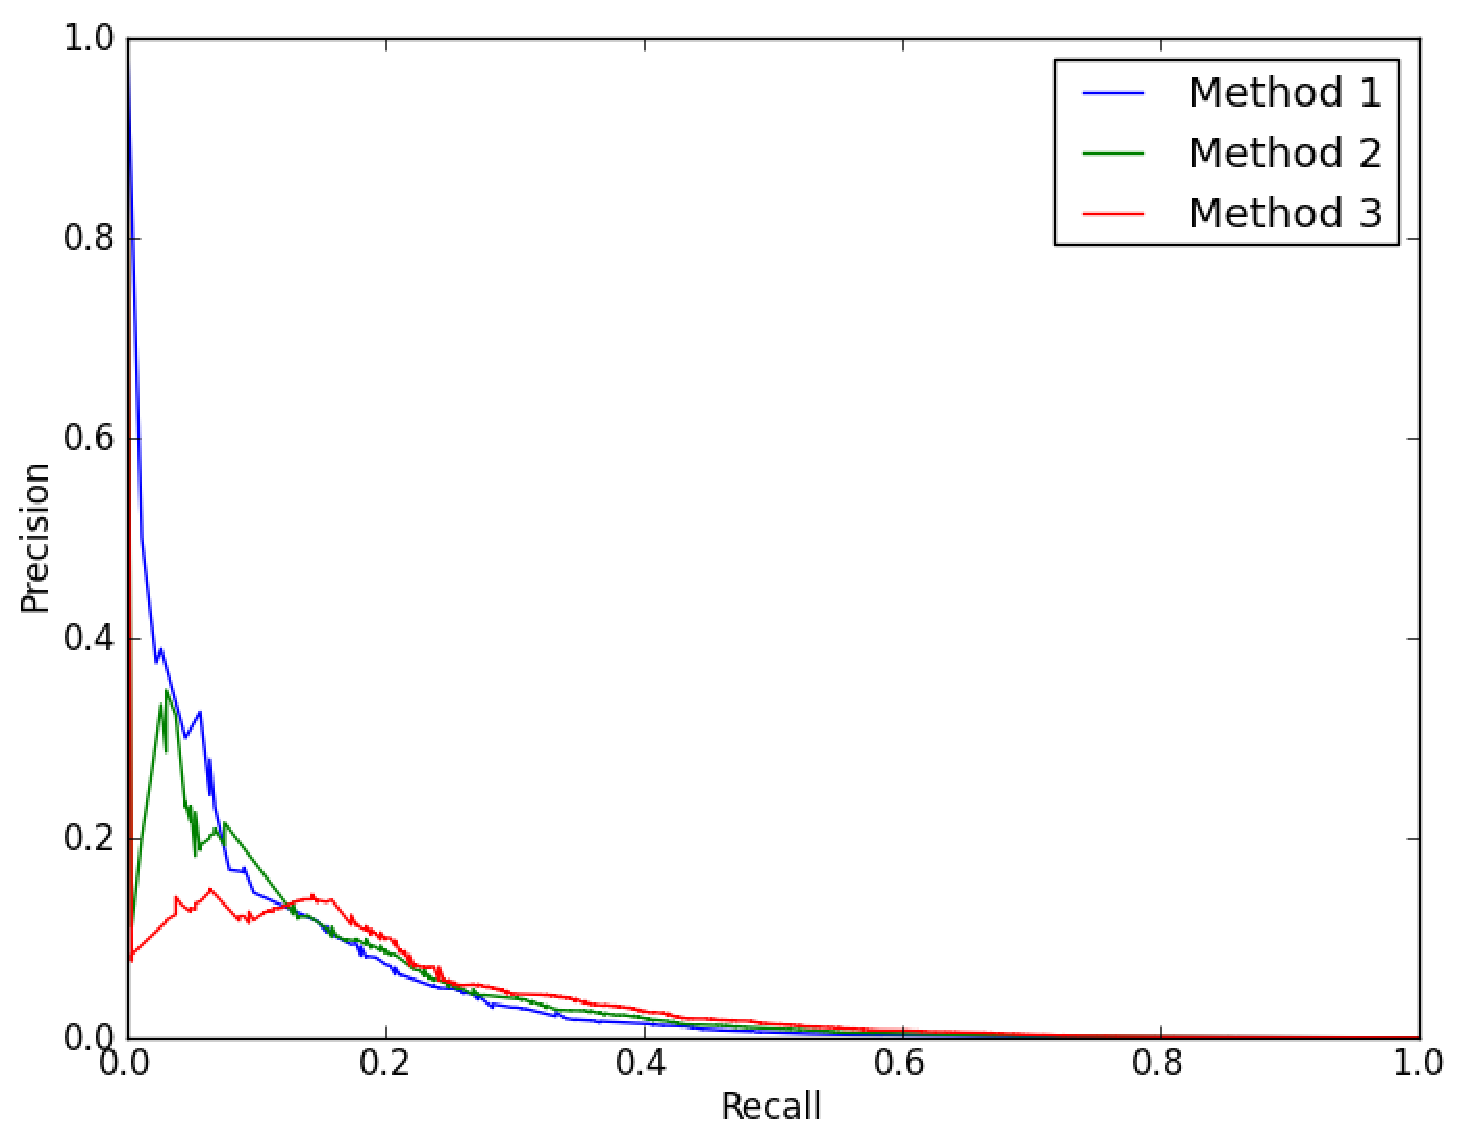
\includegraphics[width=0.95\textwidth, height = 8cm]{figures/prcurve.eps}
        \caption{PR曲线}\label{fig:prcurve}
    \end{minipage}
    \begin{minipage}[t]{0.49\linewidth}
        \centering
        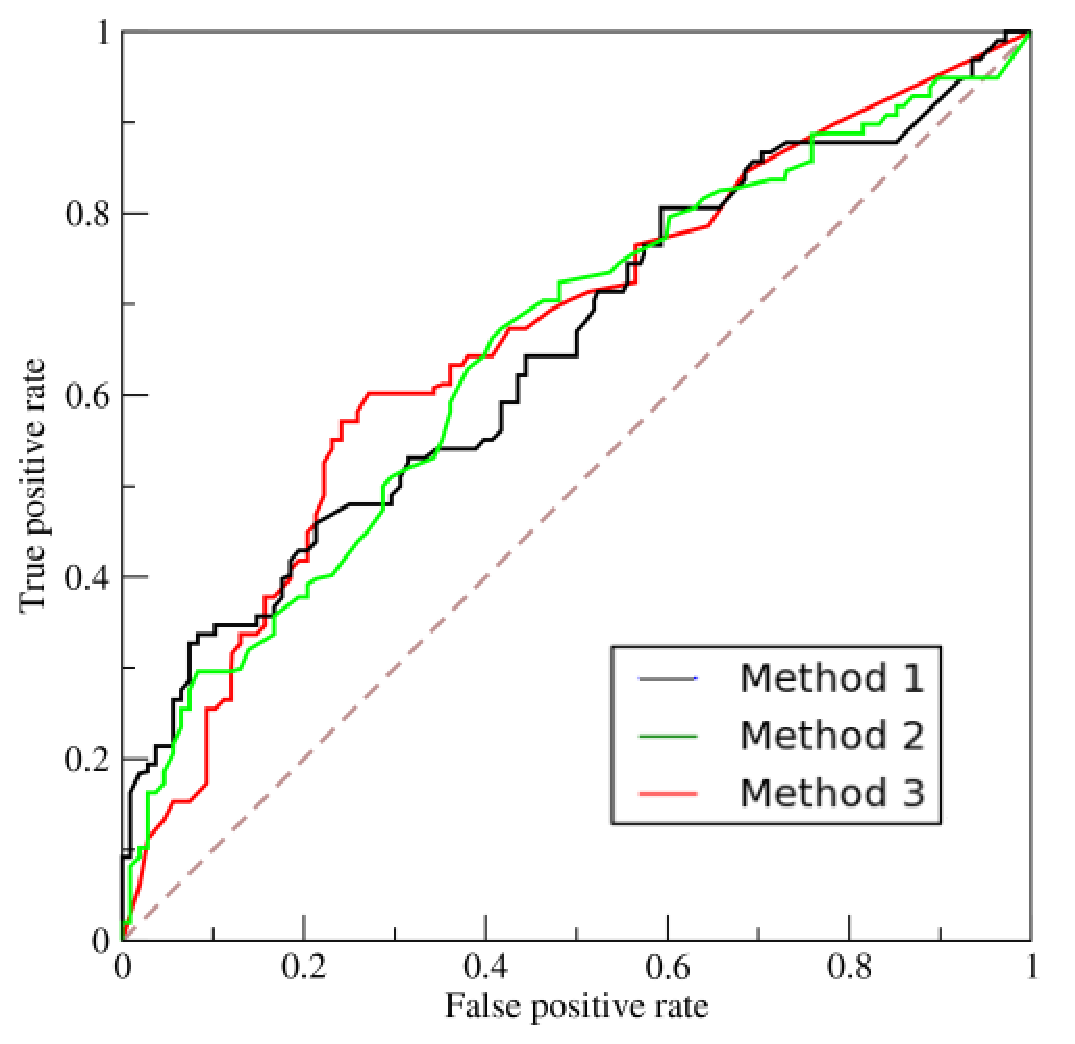
\includegraphics[width = 0.95\textwidth, height = 8cm]{figures/roccurve.eps}
        \caption{ROC曲线}\label{fig:roccurve}
    \end{minipage}
\end{figure}

为了融合查准率与查全率两种指标,学术界提出了如下定义的F度量(F-Measure):
\begin{equation}\label{eq:fmeasure}
  \text{F} = \frac{1}{\lambda\frac{1}{\text{P}} + (1-\lambda)\frac{1}{\text{R}}}
\end{equation}
其中,P表示查准率,R表示查全率,$\lambda \in (0,1)$平衡两个指标的作用,通常取$\lambda=0.5$,则有:
\begin{equation}\label{eq:0.5fmeasure}
  \text{F} = \frac{2\text{PR}}{\text{P+R}}
\end{equation}
此时,又称F度量为$F_1$度量。

ROC曲线(受试者工作特征——Receiver Operator Characteristic)源于信号检测理论,并广泛应用于机器学习和数据挖掘领域,是模型选择与评估的一个重要工具。在二元分类问题中,研究人员使用ROC曲线形象地刻画分类模型的假阳性率(横轴)与真阳性率(纵轴)之间的关系。对于完全随机分类模型,其ROC 曲线是连接原点与$(1,1)$ 的45°角平分线,任何优于随机分类的模型,其ROC曲线都位于45°平分线上方(见图\ref{fig:roccurve})
\footnote{在讨论ROC与PR曲线时,可能涉及到凸壳(Convex Hull),也称凸包(Convex Envelop)的概念,简单而言,在实数向量空间$V$中,对于给定集合$X$的凸包$S$ 是指$V$中所有包含$X$的凸集$K$的交:\[S = \bigcup\limits_{X\subseteq K \subseteq V} K,\]如果$X$是有限的,则$X$的凸包可以由$X$内所有点$(x_1,\ldots,x_n)$ 线性组合来构造:\[S = \{\sum\limits_{i = 1}^n \alpha_i x_i \mid x_i\in X, \sum\limits_{i = 1}^n \alpha_i = 1, \alpha_i \in [0,1]\}\]}。
ROC曲线下方面积AUC\cite{bradley1997use}可用来衡量模型预测的准确性,指标范围在$[0,1]$之间,有趣的是AUC同Wilcoxon-Mann-Whitney统计量是等价的~\cite{hanely1982meaning},可用于衡量分类模型的排名性能。

\subsection{平均精度均值}
根据精度的定义,可以定义平均精度(Average Precision):
\begin{equation}\label{eq:ap}
    \text{AP}=\frac{1}{n_1} \sum_{k=1}^{n}{I(y_{\pi^{-1}(k)}=1)\text{P@k}}
\end{equation}
其中,$n$是与检索词关联的文档数目,$n_1$表示相关文档的数目,在PR曲线中,平均精度近似地等于曲线下方面积所占比例。

平均精度均值(Mean Average Precision,MAP)是指所有检索词上的AP的平均值,即
\begin{equation}\label{eq:map}
    \text{MAP} = \frac{1}{|Q|}\sum_{q\in Q}{\text{AP}(q)}
\end{equation}

\subsection{折损累积增益}
折损累积增益(Discounted Cumulative Gain,DCG)是评价排名质量的一种标准指标,常用于度量搜索排名算法的精度,在信息检索领域有广泛使用。它不局限于评价仅含有相关、不相关两种评分相关等级的排名问题,对于包含多个评分相关等级的排名问题同样适用。给定一个排名列表,折损累积增益根据文档在排名列表中的位置信息计算其有用性或称增益量,从排名列表的顶部到底部累积各个位置的增益量,并以各自的位置信息进行折损。一般地,如果相关性越高则越有用,相应地在排名列表中的位置越靠前,则折损累积增益的值就越高。在评价排序模型的质量时,如果折损累积增益的值越大,则认为排序模型性能越高。

在折损累积增益诞生之前,常使用一种称为\textbf{累积增益}的指标,它只是将对应位置以后所有对象的评分相关等级机械相加,没有将位置信息计入增益量。对于给定的排名列表$\pi$,在位置$k$处的累积增益定义如下:
\begin{equation}
    \text{CG@k} = \sum\limits_{i=1}^k y_{\pi^{-1}(i)}
\end{equation}
其中,$\pi^{-1}(i)$表示在排名列表中排在位置$i$的对象,其相关等级用$y_{\pi^{-1}(i)}$表示。在累积增益的计算过程中,如果调换排名在$[1,k]$范围内任意两个对象的位置,无论是将相关的对象位置往后挪,还是将不相关对象的位置向前移,都不会影响累积增益量。折损累积增益克服了累计增益的这一缺陷,对于不同位置的增益设置不同的折损:位置靠前的对象折损越小,有用性更高。对于位置$k$处的折损累积增益定义如下:
\begin{equation}
    \text{DCG@k} = y_{\pi^{-1}(1)} + \sum\limits_{i=2}^k \frac{y_{\pi^{-1}(i)}}{\log i}
\end{equation}
或者
\begin{equation}
    \text{DCG@k} = \sum\limits_{i=1}^k \frac{2^{y_{\pi^{-1}(i)}}-1}{\log (i+1)}
\end{equation}
其中,公式加和项分数的分子部分表示\textbf{增益},分母部分表示\textbf{折损}。通过选择不同截断位置(Cut-off),折损累积增益可以评价不同位置上的排名质量。

在网络搜索应用中,由于不同搜索引擎所使用的排名算法不同,对于同一个检索词,每个系统返回的搜索结果数量也不相同。为方便比较不同搜索引擎、不同排名算法,需要对折损累积增益在检索词上做标准化处理。假设对于每一个检索词,都存在一个真实的排名列表,如果某个排序模型的预测排名与真实排名完全一致,我们称之为理想排名模型,相应排名结果称为\textbf{理想排名},而根据理想排名列表计算的折损累积增益也称\textbf{理想累积增益}。理想累积增益在位置$k$截断值记作$Z_k$,利用它标准化折损累积增益就得到\textbf{标准累积增益}:
\begin{equation}
    \text{NDCG@k} = \frac{\text{DCG@k}}{Z_k}
\end{equation}
取值范围在$[0,1]$,它是评价排序模型或算法质量最常用的一种标准指标。

\subsection{倒数排名均值}
倒数排名均值(Mean Reciprocal Rank,MRR)是一种衡量两个级别的排名质量的度量方式,是倒数排名(Reciprocal Rank, RR)在检索词集合$Q$上的平均值。倒数排名是指对于某个检索词,相关文档最好的排名,即$\mathrm{RR}=r^{-1}$,$r$表示与检索词相关的文档最好的排名。比如,某个检索词的相关文档只有2个,其中一个排在第2位,另一个排在第10 位,那么其倒数排名为$2^{-1}$。对所有检索词的倒数排名取均值,就是平均倒数排名:
\begin{equation}\label{eq:mrr}
    \text{MRR}=\frac{1}{|Q|}\sum_{q\in Q}{\frac{1}{r_q}}
\end{equation}

\subsection{倒数排名期望}
倒数排名期望(Expected Reciprocal Rank,ERR)由Chapelle等人\cite{chapelle2009expected}提出,通过用户对搜索结果满意程度的统计模型分析,ERR表现优于DCG度量。

假设位置$j$的文档让用户满意的概率为$R_j$,则用户在位置$r$找到心仪的文档并停止浏览和查找的概率为:
\[
    \prod_{j=1}^{r-1}{(1-R_j)R_r}
\]
一般地,$R_j$可以使用对应位置文档的等级表示:
\[
    R_j=\frac{2^{y_j}-1}{2^{y_{\max}}}
\]

ERR可以定义为下式:
\begin{equation}\label{eq:err}
    \text{ERR} = \sum_{r=1}^{n} \frac{1}{r}\prod_{j=1}^{r-1}{(1-R_j)}R_r
\end{equation}
其中$n$表示待排名的文档数目;$y_i$表示排在$i$的文档等级;$y_{\max}$表示文档的最高等级。

\subsection{pFound}
pFound由Gulin等人\cite{gulin2009pfound}提出,Yandex从2007年就开始用它来评估搜索效果。与ERR类似,pFound也是一种衡量用户满意程度的概率模型。
\begin{equation}\label{eq:pfound}
    \text{pFound} = \sum_{r=1}^{n}{\prod_{j=1}^{r-1}{(1-b)(1-R_j)R_r}} = \sum_{r=1}^{n}{(1-b)^{r-1}}\prod_{j=1}^{r-1}{(1-R_j)R_r}
\end{equation}
$R_j$与ERR中的含义相同,表示用户在$j$处找到满意文档的概率;$b$表示在各个位置停止查找的概率,默认取值0.15。

ERR和pFound都基于相同的假设:(i)用户从上到下逐个浏览搜索结果页面;(ii)用户逐个点击搜索结果,直到找到目标文档或者没有找到而放弃搜索。

\subsection{胜者全拿}
胜者全拿(Winner Takes All,WTA)是一种两级别度量,对于某个检索词,如果排名最前的文档与之相关,则WTA损失为0,否则为1。

\section{信息度量}
信息论是运用概率论与数理统计的方法研究信息、信息熵、通信系统、数据传输、密码学、数据压缩等问题的应用数学学科。Shannon和Weaver于1948年10月发表在《贝尔系统技术学报》的论文\textbf{通信的数学原理}\cite{shannon1948mathematical},可以视作是现代信息论研究的开端。Claude Shannon由于在信息理论中的突出贡献被后人尊称为“信息论之父”。

\begin{figure}[htbp]
\begin{minipage}[h]{0.33\linewidth}
\centering
  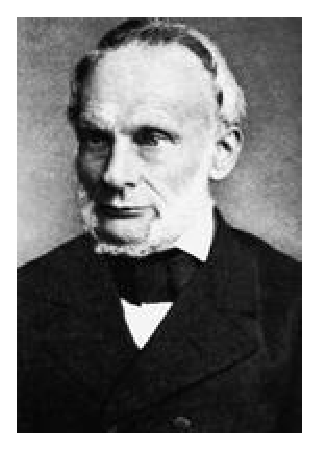
\includegraphics[width=0.9\textwidth, height=7cm]{figures/scientists/RudolfClausius.eps}
  \label{fig:RudolfClausius}
\end{minipage}
\begin{minipage}[h]{0.33\linewidth}
\centering
  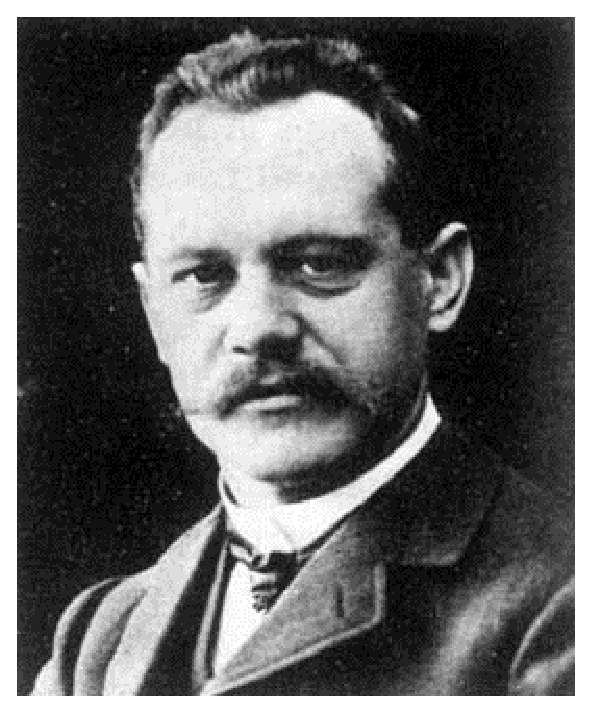
\includegraphics[width=0.9\textwidth, height=7cm]{figures/scientists/LudwigBoltzmann.eps}
  \label{fig:LudwigBoltzmann}
\end{minipage}
\begin{minipage}[h]{0.33\linewidth}
\centering
  \includegraphics[width=0.9\textwidth, height=7cm]{figures/scientists/claudeshannon.eps}
  \label{fig:claudeshannon}
\end{minipage}
\caption{Left:Rudolf Clausius (1822 - 1888), Middle:Ludwig Boltzmann (1844 - 1906), Right:Claude Shannon (1916 - 2001)}
\end{figure}

信息论将信息的传递作为一种统计现象来考虑,给出了估算通信信道容量的方法。信息传输和信息压缩是信息论研究中的两大领域,二者又通过信道编码定理、信源-信道隔离定理相互联系。信源编码和信道编码是信息论的基本研究课题。

\subsection{熵}
19世纪60年代,德国物理学家Rudolf Clausius在研究实际热机中发现,实际热机工作时会产生“无法使用”的热量(如摩擦产生的热量),并首次提出“熵
(Entropy)”的概念,用来描述能量的耗散。19世纪70 年代,Ludwig Boltzmann在分析系统中微观粒子的统计行为时给出熵的统计学定义,并证明这种统计学意义上的熵与Cluasius给出的热力学熵是等价的,仅仅相差一个常数项(Boltzmann常数)。根据熵的统计学定义,热力学第二定律说明一个孤立系统倾向于混乱程度增加(即“熵增”)。

受此启发,Shannon和Weaver在\cite{shannon1948mathematical} 中提出信息熵(Information Entropy,简称“熵”)的概念,并证明熵与信息的不确定性存在等价关系,信息熵越大,意味着不确定性越大,从而事件所包含的信息量越大。

离散随机变量$X=\{x_1,\ldots,x_n\}$的熵用于度量隐含于变量$X$的值的不确定性程度,如果令$p(x)$表示$X=x$的概率,那么变量$X$的熵定义为:
\begin{equation}\label{eq:entropy}
  H(X) = E_X[I(x)] = -\sum_{x\in X}{p(x)\log p(x)}
\end{equation}
其中,$I(x)$表示单个信息的熵分布,有时称作\textbf{自信息}(Self Information),$E_X$表示期望。计算中使用的对数基底如果是2,熵的单位就是比特(bit),在用符号表达信息时,熵用来量化单个字符可以存储或传输的平均比特数。

如果随机变量$X$是连续的,则熵可以使用积分计算
\begin{equation}\label{eq:continualentropy}
  H(X) = -\int_x{p(x)\log p(x)}dx.
\end{equation}
根据连续随机变量$X$熵的定义,我们可以计算常见连续分布的熵,比如$X\sim N(\mu,\sigma^2)$,则其连续熵
\[
\begin{array}{lcl}
    H(X) &=& -\int_{-\infty}^{+\infty} \frac{1}{\sqrt{2\pi}\sigma} \exp\{-\frac{(x-\mu)^2}{2\sigma^2}\} \big[-\frac{(x-\mu)^2}{2\sigma^2} - \log \big(\sqrt{2\pi}\sigma\big)\big]dx\\
    &=&\log \big(\sqrt{2\pi}\sigma\big) \int_{-\infty}^{+\infty} \frac{1}{\sqrt{2\pi}\sigma} \exp\{-\frac{(x-\mu)^2}{2\sigma^2}\} dx + \frac{1}{2\sigma^2} \int_{-\infty}^{+\infty}(x-\mu)^2 \frac{1}{\sqrt{2\pi}\sigma} \exp\{-\frac{(x-\mu)^2}{2\sigma^2}\} dx\\
    &=& \frac{1}{2} \big[1 + \log(2\pi \sigma^2)\big],
\end{array}
\]
由此可以看出,服从正态分布的变量,其熵的大小只与方差有关,方差相同则对应的熵也相等,方差越大熵值越大。

\begin{theorem}
对于随机变量$X$,$H(X)\ge 0$,当且仅当随机变量服从均匀分布时,$H(X)$最大。对于离散变量$X$,如果它的可能取值为有限集合$\{x_1,\ldots,x_n\}$,则有$H(X) \le \log n$,当且仅当$p(x_i)=\frac{1}{n}$时,等式成立。
\end{theorem}

\subsection{联合熵}
如果将两个离散随机变量$X$和$Y$简单联合,构成新的联合随机变量$(X,Y)$,则新的联合随机变量的熵(Joint Entropy)定义为:
\begin{equation}\label{eq:jointentropy}
  H(X,Y) = E_{X,Y}[I(x,y)] = -\sum_{x,y}{p(x,y)\log p(x,y)}
\end{equation}

如果事件$X$和$Y$是相互独立的,则$p(x,y)=p(x)p(y)$,那么
\[
  H(X,Y) = -\sum_{x,y}{p(x)p(y)\log(p(x)p(y))}= -\sum\limits_{x} p(x)\log p(x)-\sum\limits_y p(y)\log p(y)=H(X) + H(Y)
\]
\subsection{交叉熵}
假设随机变量$X$的概率密度函数为$P(X)$,许多情况下$P(X)$是未知的,人们通常使用统计的手段得到$P(X)$的近似分布$Q(x)$,则随机变量$X$的交叉熵(Cross Entropy)定义为:
\begin{equation}\label{eq:crossentropy}
  H(P(X),Q(X)) = -\sum_{x\in X}{P(x)\log Q(x)}
\end{equation}

如果将交叉熵引入计算机语言学,可以处理机器翻译的歧义问题。采用语句的真实语义作为交叉熵的训练集的先验信息,将机器翻译的语义作为测试集后验信息,使用两者的交叉熵指导对歧义的辨识和消除。
\subsection{条件熵}
设有随机变量$X,Y$,其联合概率分布为
\[
    p(x,y) = P(X=x, Y = y)
\]
条件熵(Conditional Entropy)$H(X|Y)$表示已知随机变量$Y$的条件下,随机变量$X$的不确定性,并做如下定义:
\begin{equation}\label{eq:conditionalentropy}
    \begin{array}{lll}
        H(X\mid Y) & = & E_Y[H(X|Y=y)] \\
         & = & \sum\limits_y p(y) H(X|Y=y)\\
         & = & -\sum\limits_y p(y)\sum\limits_x{p(x|y)\log p(x|y)} \\
         & = & -\sum\limits_{x,y} p(x,y)\log\frac{p(x,y)}{p(y)} \\
         & = & H(X,Y) - H(Y)
    \end{array}
\end{equation}
$H(X|Y)$表示随机变量$Y$给定条件下,$X$的条件概率分布熵在$Y$上的数学期望。

\subsection{KL散度}
KL散度(Kullback–Leibler Divergence)\cite{kullback1951information,kullback2012information},又称相对熵(Relative Entropy)或信息散度(Information Divergence)是度量两分布(真实概率分布与任意概率分布)之间距离的一种方式。假设存在某真实分布$p(X)$ 及任意一个分布$q(X)$,则两分布之间的KL散度定义为:
\begin{equation}\label{eq:relativeentropy}
  D_{KL}(p(X)\|q(X)) = \sum_{x\in X}{p(x)\log\frac{p(x)}{q(x)}}
\end{equation}
根据交叉熵的定义可知:
\begin{equation}
    D_{KL}(p(X)\|q(X)) = \sum_{x\in X}{p(x)\log\frac{p(x)}{q(x)}} = -\sum_{x\in X}{p(x)\log q(x)} - H(X) = H(p(X),q(X)) - H(X)
\end{equation}

\begin{lemma}
对任意两个分布$p(X)$与$q(X)$,都有$D_{KL}(p(X)\|q(X))\ge 0$,当且仅当$p(X)=q(X)$时,$D_{KL}(p(X)\|q(X))= 0$。
\end{lemma}
\begin{lemma}[Pythagorean性质]
如果$p\in P$,$q\in Q$,$\hat p\in P\cap Q$,则有
\[
    D_{KL}(p(X)\|q(X))=D_{KL}(p(X)\|\hat p(X)) + D_{KL}(\hat p(X)\|q(X)).
\]
\end{lemma}

\begin{theorem}[最大熵解]
如果$\hat p\in P\cap Q$,则解
\begin{equation}
    \hat p = \argmax\limits_{p} H(p)
\end{equation}
存在且唯一。
\end{theorem}

\begin{theorem}[最大似然解]
如果$\hat p\in P\cap Q$,则解
\begin{equation}
    \hat p = \argmax\limits_{q} L(q)
\end{equation}
存在且唯一。
\end{theorem}

\begin{theorem}[对偶定理]
存在唯一的分布$\hat p$,满足
\begin{equation}
    \hat p = \argmax\limits_{p} H(p) = \argmax\limits_{q} L(q) \in P\cap Q.
\end{equation}
\end{theorem}
根据对偶定理可知,最大熵解可以写作对数线性形式,解出最大似然解就给出了最大熵解。

\begin{figure}[htbp]
\begin{minipage}[h]{0.49\linewidth}
\centering
  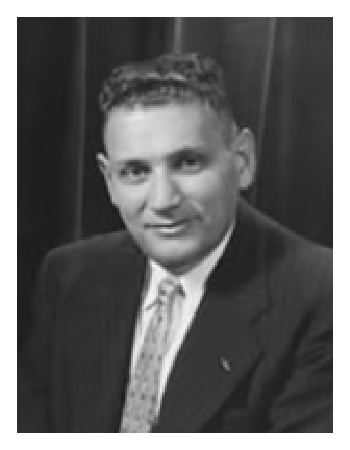
\includegraphics[width=0.95\textwidth, height=9cm]{figures/scientists/SolomonKullback.eps}
  \caption{Solomon Kullback (1907 - 1994)}\label{fig:SolomonKullback}
\end{minipage}
\begin{minipage}[h]{0.49\linewidth}
\centering
  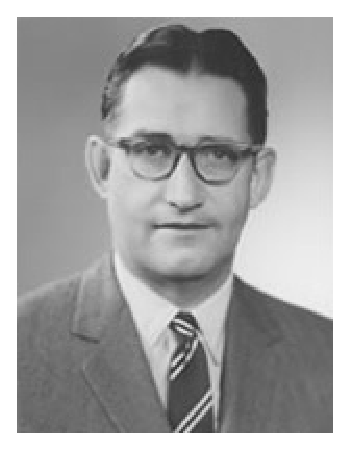
\includegraphics[width=0.95\textwidth, height=9cm]{figures/scientists/RichardLeibler.eps}
  \caption{Richard Leibler (1904 - 2003)}\label{fig:RichardLeibler}
\end{minipage}
\end{figure}

在数据压缩应用中,假设数据服从分布$q(X)$并执行压缩,而数据真实分布为$p(X)$,则KL-散度表示相对理想情况,压缩数据需要的平均额外的支出(比特)。
从信息论的角度来看,如果随机变量的真实分布为$p(X)$,然而人们却错误地使用概率密度函数$q(X)$,则KL散度刻画了由于使用错误的分布密度函数而导致信息量的增加。

\subsection{互信息}
互信息(Mutual Information)表示通过观察一个随机变量,从另外一个随机变量中获取的信息量,它是通信理论中的一个重要指标,常用于最大化发送信号和接收信号间共享的信息量。随机变量$X$相对$Y$的互信息定义为:
\begin{equation}\label{eq:mutualinfo}
  I(X;Y) = \sum_{X,Y}{p(x,y)\log\frac{p(x,y)}{p(x)p(y)}} = H(X) - H(X|Y) = H(X) + H(Y) - H(X,Y)
\end{equation}
由此可知,在知道$Y$的情况下为$X$编码,相比不知道$Y$的情况下,可以节省$I(X;Y)$个比特。由定义可知,互信息$I(X;Y)$是对称的。如果随机变量$X$和$Y$是相互独立的,由$H(X,Y)=H(X) + H(Y)$可知$I(X;Y)=0$。

根据等式
\[
 D_{KL}(p(X|Y=y)\| p(X)) = \sum_{x\in X}{p(x|y)\log\frac{p(x|y)}{p(x)}}=\sum_{x\in X}{p(x|y)\log\frac{p(x,y)}{p(x)p(y)}}
\]
可以使用KL-Divergence表示互信息:
\[
    I(X;Y) = \sum_{x\in X}{p(x|y)p(y)\log\frac{p(x,y)}{p(x)p(y)}} = E_{p(y)}[D_{KL}(p(X|Y=y)\|p(X))]
\]
联合熵、条件熵、互信息三者之间的关系可以通过图\ref{fig:entropy}形象表示。
\begin{figure}[ht]
  \centering
  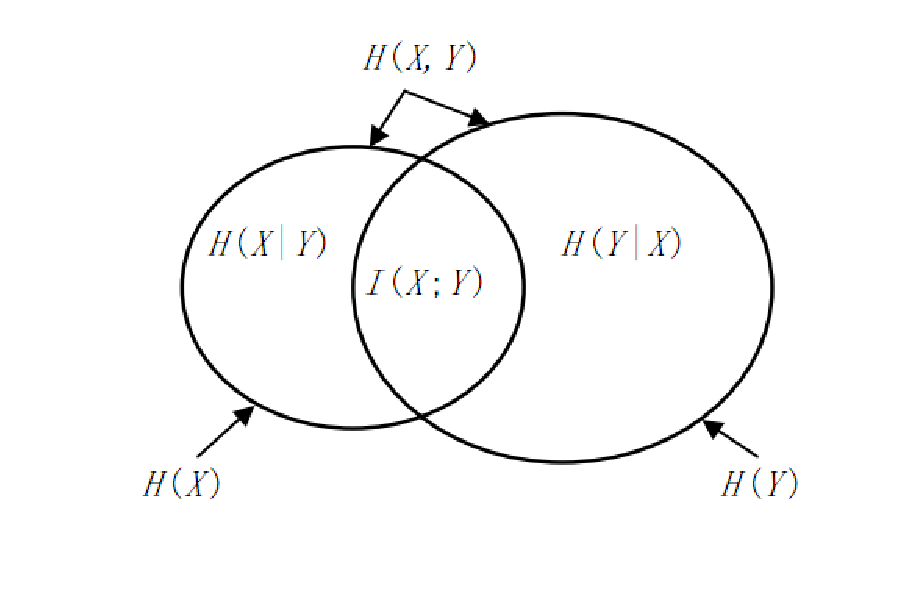
\includegraphics[width=0.6\textwidth]{figures/entropy.eps}
  \caption{联合熵、条件熵、互信息三者之间的关系}\label{fig:entropy}
\end{figure}

\subsection{詹森--香农散度}
詹森--香农散度(Jensen--Shannon Divergence),也称信息半径(Information Radius,IRad),在统计学中,常用作衡量两个概率分布的相似度。JS散度建立在KL散度之上,但又不同于KL散度:JS散度是对称的。它最初为Dagan Ido等人用于计算单词的相似性\cite{dagan1999similarity},现在已经成为生物信息学重要的度量工具。

对于两个概率分布$P$与$Q$,它们的JS散度定义为两个KL散度的均值:
\begin{equation}
  D_{JS}(P\| Q) = \frac{1}{2}(D_{KL}(P\| M) + D_{KL}(Q\| M))
\end{equation}
其中,$M = (P + Q)/2$表示$P,Q$的混合概率分布。根据定义可知$D_{JS} \in [0,1]$:
\begin{equation}
\begin{array}{ll}
  D_{JS}(P\| Q) & = \frac{1}{2}(\sum P\log{\frac{P}{M}} + \sum Q\log{\frac{Q}{M}})\\
   & = H(M) - \frac{1}{2}H(P) - \frac{1}{2}H(Q)
\end{array}
\end{equation}

假设$X$是服从混合分布$M$的随机变量,$Z$表示二元示性变量(Binary Indicator Variable),如果$X$服从$P$时,则$Z=1$,如果$X$服从$Q$时,则$Z=0$。变量$X$与$Z$的互信息
\begin{equation}
\begin{array}{ll}
  H(X;Z) & = H(X) - H(X|Z)\\
   & = \sum M\log M - \prob(Z = 0) H(X|0) - \prob(Z = 1)H(X|1)\\
   & = H(M) - \frac{1}{2}H(P) - \frac{1}{2}H(Q)
\end{array}
\end{equation}
与概率分布$P$和$Q$的JS散度等价。

\subsubsection{最小编码长度}
哈夫曼编码是由戴维·哈夫曼David A. Huffman于1952年提出,属于一种典型的变长编码(Variable Length Coding, VLC)方式,基于“高频字母短编码,低频字母长编码”的原则实现最优编码,主要用于文本文件的无损压缩(Lossless Compression)。
\begin{figure}[t]
  \centering
  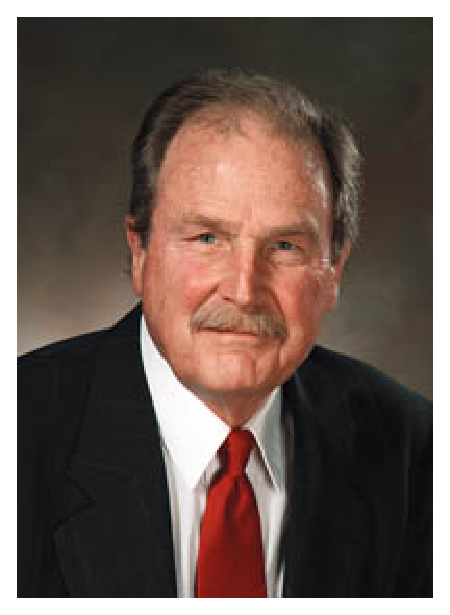
\includegraphics[width=0.3\textwidth, height = 7cm]{figures/scientists/DavidHuffman.eps}\\
  \caption{David Albert Huffman (1925 - 1999)}\label{fig:DavidHuffman}
\end{figure}

哈夫曼编码的目标是寻找最有效率的编码方式,使得平均编码长度最短。可以证明哈夫曼编码是满足最小信息熵的编码。
\subsubsection{Fano不等式}
%-----------metrics
\part{数学基础}
\chapter{矩阵论}
矩阵是高等代数学中的一个常见工具,也常见于统计学、物理学、计算机科学等学科。矩阵运算是数值分析领域的一个重要问题,将矩阵分解为简单矩阵的组合可以在理论和实际应用中简化矩阵运算。一些应用广泛而形式特殊的矩阵,如稀疏矩阵和准对角矩阵,都有特定的快速运算方法。

假设矩阵$A$是$m\times n$维的实数矩阵,则$A\in \mathbb R^{m\times n}$,并记$A^T$为$A$的\textbf{转置矩阵}(Transpose Matrix)。如果$m=n$,则称$A$为方块矩阵,简称方阵,并记$|A|$ 或$\textit{det}(A)$为其\textbf{行列式}(Determinant)。如果方阵$A\in \mathbb R^{n\times n}$对称,则有$A^T=A$,比如非对角元都是零元的\textbf{对角阵}(Diagonal Matrix)。如果对角阵对角元都是$1$,则称其为\textbf{单位矩阵}(Identity Matrix),并记作$I$。如果$A$\textbf{可逆}
(Invertible),记$A^{-1}$为其\textbf{逆矩阵}(Inverse Matrix),则有$AA^{-1} = A^{-1}A=I$,此时$A$也被称作\textbf{非奇异阵}(Nonsingular Matrix),并且满足$|A|\ne 0$。方阵$A$ 所有对角元素之和称作矩阵$A$ 的\textbf{迹}(Trace),记作$\tr(A)=\sum\limits_i a_{ii}$。

\begin{definition}[分块矩阵]
如果矩阵$A\in \mathbb R^{m\times n}$,利用矩阵行或列向量,可分块表示成如下两种形式:
\[
    \left\{
        \begin{array}{rcl}
          A &=& [A_{\bullet 1}, A_{\bullet 2}, \ldots, A_{\bullet n}],\\
          A &=& [A_{1 \bullet}, A_{2 \bullet}, \ldots, A_{m \bullet}]^T,
        \end{array}
    \right.
\]
其中,$A_{\bullet i}=[a_{1i},\ldots,a_{mi}]^T \in \mathbb R^m$为矩阵$A$的第$i$列,$A_{i\bullet}=[a_{i1},\ldots,a_{in}]\in \mathbb R^{1\times n}$ 是$A$的第$i$行。
\end{definition}

%\begin{definition}[矩阵向量化]
%\textbf{矩阵向量化}(Matrix Vectorization)是一种将矩阵转换为列向量的线性变换:逐列将矩阵的行元顺次堆成一列。对于矩阵$A\in \mathbb R^{m\times n}$,其向量化定义如下
%\begin{equation}
%    \vect(A) = [A_{\bullet 1}^T, A_{\bullet 2}^T, \ldots, A_{\bullet n}^T]^T \in \mathbb R^{mn}.
%\end{equation}
%\end{definition}
%
%\begin{definition}[克罗内克积]
%假设$A\in \mathbb R^{m\times n}$,$X\in \mathbb R^{p\times q}$,则$A$和$X$的\textbf{克罗内克积}(Kronecker Product)为
%\begin{equation}
%    A \otimes X =
%    \begin{bmatrix}
%        a_{11} X & a_{12} X & \cdots & a_{1n} X\\
%        a_{21} X & a_{22} X & \cdots & a_{2n} X\\
%        \vdots & \vdots & \ddots & \vdots\\
%        a_{m1} X & a_{m2} X & \cdots & a_{mn} X\\
%    \end{bmatrix}=\big[a_{ij} X\big]\in \mathbb R^{mp \times nq}.
%\end{equation}
%\end{definition}

\section{特征系统}

\subsection{特征值与特征向量}
\begin{definition}
对于矩阵$A\in \mathbb C^{n\times n}$,如果存在$\lambda\in \mathbb C$与非零向量$\omega\in \mathbb C^n$,满足$A\omega=\lambda \omega$,则称$\lambda$是矩阵$A$ 的一个\textbf{特征值}(Eigenvalue),$\omega$是其对应\textbf{特征向量}(Eigenvector)。矩阵$A$对应于复空间$\mathbb C^{n\times n}$上的一个线性变换。
\end{definition}

\begin{definition}
如果矩阵$A\in \mathbb C^{n\times n}$存在特征值$\lambda_1,\ldots,\lambda_n$,则矩阵$A$的\textbf{谱半径}(Spectral Radius)有定义:
\begin{equation}
    \rho(A) = \max\limits_{1\le i\le n} |\lambda_i|.
\end{equation}
如果特征值满足关系$|\lambda_1| > |\lambda_2| \ge \dots \ge |\lambda_n|$,则称$\lambda_1$为$A$的\textbf{主特征值},其对应特征向量$\omega_1$为$A$的
\textbf{主特征向量},矩阵$A$的谱半径$\rho(A)=|\lambda_1|$。
\end{definition}

\begin{proposition}
如果矩阵$A$存在特征值$\lambda_1,\ldots,\lambda_n$,则特征值满足:
\begin{eqnarray}
  \sum\limits_i \lambda_i &=& \tr(A), \\
  \prod\limits_i \lambda_i &=& |A|.
\end{eqnarray}
如果特征值彼此不相同,则对应特征向量$\omega_1,\ldots, \omega_n$也线性无关。
\end{proposition}

\begin{definition}[Gershgorin圆盘]
对于矩阵$A\in \mathbb C^{n\times n}$,如果记$r_i=\sum\limits_{j\ne i} |a_{ij}|$,$1\le i\le n$,我们称
\begin{equation}
    D(a_{ii}; r_i) = \bigg\{z\in \mathbb C \bigg| |z - a_{ii}| \le r_i\bigg\}
\end{equation}
是矩阵$A$的\textbf{Gershgorin圆盘}(Gershgorin Disc)。
\end{definition}

\begin{theorem}[Gershgorin圆盘定理]
复数域上矩阵的任意特征值都至少落在一个Gershgorin圆盘内。
\end{theorem}

\begin{definition}[矩阵范数]
如果矩阵$A\in \mathbb R^{m\times n}$,则它存在如下几种形式的范数$\|A\|$:
\begin{itemize}
  \item $\|A\|_1=\max\limits_{1\le j\le n} \sum\limits_{i=1}^m |a_{ij}|$表示矩阵的最大列和(绝对值),称作\textbf{列和范数}。
  \item $\|A\|_2=\sigma_1(A)=\sqrt{\rho(A^T A)}$,表示矩阵最大的奇异值,称作\textbf{谱范数}。
  \item $\|A\|_{\infty}=\max\limits_{1\le i\le m} \sum\limits_{j=1}^n |a_{ij}|$,表示矩阵的最大行和(绝对值),称作\textbf{行和范数}。
  \item $\|A\|_{\mathcal F}=\sqrt{\tr(A^T A)}=\sqrt{\sum\limits_{i=1}^m \sum\limits_{j=1}^n |a_{ij}|^2}$,称作\textbf{Frobenius范数}。
  \item $\|A\|_{\star}=\sum\limits_i \sigma_i(A)$,表示矩阵奇异值之和,称作\textbf{核范数}。
\end{itemize}
\end{definition}

\begin{theorem}\label{th:spectral-radius-norm}
任意复数域上的矩阵,其谱半径不大于其任意一种诱导范数。

\begin{proof}
假设矩阵$A\in \mathbb C^{n\times n}$的特征值为$\lambda_i$,$1\le i \le n$。任选一个特征值$\lambda\in\{\lambda_1,\ldots,\lambda_n\}$,设$\omega\ne 0$是对应特征向量。我们构造矩阵$X=[\omega,0,\ldots,0]\in \mathbb C^{n\times n}$,则$\|X\|\ne 0$且$AX=\lambda X$。根据矩阵范数的一致性(也称次可乘性)
\[
    |\lambda|\|X\|=\|AX\| \le \|A\|\|X\|
\]
可知$|\lambda\|\le \|A\|$。由$\lambda$的任意性证得$\rho(A)\le \|A\|$,即$A$的谱半径是其任意一种诱导范数的下界。
\end{proof}
\end{theorem}

\subsection{二次型}
\begin{definition}
多元变量$x_1,\ldots,x_n$的\textbf{二次型}(Quadratic Form)是形如
\begin{equation}
    Q(x) = a_{11} x_1^2 +\cdots + a_{ij} x_i x_j + \cdots + a_{nn} x_n^2 = \sum\limits_{1\le i\le n}\sum\limits_{1\le j \le n} a_{ij} x_i x_j = x^T A x
\end{equation}
的$n$元二次函数,其中$A=(a_{ij})_{n\times n}$是一个二次型矩阵。
\end{definition}

二次型矩阵$A$存在多种表示形式,比如$Q(x)=2x_1^2 + x_1x_2 + 5 x_2 x_1 - 4 x_2^2$等价于
\[
    \begin{array}{lcl}
        Q(x) & = & 2x_1^2 + 2x_1x_2 + 4 x_2 x_1 - 4 x_2^2,\\
        Q(x) & = & 2x_1^2 + 8x_1x_2 - 2x_2 x_1 - 4 x_2^2,\\
        \vdots & \vdots & \vdots\\
        Q(x) & = & 2x_1^2 + 3x_1x_2 + 3 x_2 x_1 - 4 x_2^2
    \end{array}
\]
相应地二次型矩阵也会发生变化。假设原始二次型矩阵是$A$,由于$Q(x_1,\ldots, x_n)=x^T (A + A^T) x/2$,则$(A + A^T) /2$是对称矩阵,即每个二次型都存在唯一的对称型二次型矩阵,并作为基本二次型矩阵,如前例中的基本二次型矩阵为
\[
    A =
    \begin{bmatrix}
        2 & 3\\
        3 & -4
    \end{bmatrix}.
\]

\begin{definition}
一个对称矩阵$A\in \mathbb R^{n\times n}$是\textbf{正(负)定矩阵}(Positive or Negative Definite Matrix),当且仅当对所有非零向量$x\in \mathbb R^n$都有$x^T A x>0 (<0)$。$A$ 是\textbf{半正(负)定矩阵}(Positive or Negative Semi-definite Matrix)当且仅当对所有向量$x\in \mathbb R^n$都有$x^T A x \ge 0(\le 0)$。
\end{definition}

\begin{proposition}
假设矩阵$A$的主特征向量是$\omega_1$,最小特征值对应的特征向量是$\omega_n$,则二次型$Q(x)=x^T A x$在$\omega_1$方向上变化速率最大,在$\omega_n$方向上变化速率最小。
\end{proposition}


\subsection{严格对角占优矩阵}
\begin{definition}[严格对角占优矩阵]
对于矩阵$A\in \mathbb C^{n\times n}$,如果对任意的$1\le i\le n$都有
\begin{equation}
    |a_{ii}| > \sum\limits_{j\ne i} |a_{ij}|,
\end{equation}
则称$A$是\textbf{严格对角占优矩阵}(Strictly Diagonally Dominant Matrix)。
\end{definition}

\begin{theorem}
严格对角占优矩阵是非奇异矩阵。
\end{theorem}

\subsection{随机矩阵}
\textbf{随机矩阵}(Stochastic Matrix),也称\textbf{概率矩阵}(Probability Matrix)、\textbf{转移矩阵}(Transition Matrix)或者\textbf{马尔科夫矩阵}
(Markov Matrix)是一种用以描述马尔科夫链状态转移的一种矩阵,主要应用于概率论、统计学、线性代数、金融数学及计算机领域。

\begin{definition}[随机矩阵]
对于非负矩阵$A\in \mathbb R^{n\times n}$,如果$A$的行和等于$1$,则称它为行随机矩阵或右随机矩阵,矩阵的每一行对应一个概率分布;如果矩阵$A$的列和等于$1$,则称其列随机矩阵或左随机矩阵,矩阵的每一列对应一个概率分布;如果$A$的行和与列和都等于$1$,则称其为双随机矩阵,矩阵的每一行、每一列都对应一个概率分布。
\end{definition}

\begin{theorem}
随机矩阵的主特征值是$1$。
\end{theorem}
\begin{proof}
假设矩阵$A\in \mathbb C^{n\times n}$是一个行随机矩阵,根据定理\ref{th:spectral-radius-norm}可知
\[
    \rho(A) \le \|A\|_1 = 1.
\]
由于$A \mathbf 1 = (1,\ldots, 1)^T = \mathbf 1$,表明矩阵$A$存在一个特征向量$\lambda=1$,对应特征向量是$\mathbf 1$。显然,特征值$\lambda=1$是矩阵$A$的主特征值。列随机矩阵与双随机矩阵类似可证。
\end{proof}

\subsection{特征系统的解}
\begin{algorithm}[htbp]
\caption{幂法}
\begin{algorithmic}
\REQUIRE 给定迭代次数$T$或误差阈值$\epsilon$,$t=1$,任意非零向量$x_0 \in \mathbb R^n$

\WHILE{$t<T$ 或 $\|x_t-x_{t-1}\|>\epsilon$}
\STATE $y_t = A x_{t-1}$
\STATE $x_t = y_t/{\|y_t\|}$
\STATE $t = t+1$
\ENDWHILE

\ENSURE 主特征向量$\omega_1=x_T$
\end{algorithmic}
\end{algorithm}

\begin{theorem}
如果$A\in \mathbb R^{n\times n}$是一个正定矩阵,则幂法收敛于$A$的主特征向量$\omega_1$。

\begin{proof}
如果$A$是正定矩阵,则$n$个特征向量一定线性无关,并且可以使用它们线性表示任意非零向量$x_0$,即存在非零向量$a=(a_1,\ldots,a_n)^T$,满足
\[
    x_0 = \sum\limits_i a_i \omega_i.
\]
由幂法迭代步骤可知
\[
    A^t x_0 = \sum\limits_i a_i A^t \omega_i = \sum\limits_i a_i \lambda_i^t \omega_i.
\]
对等式左右两端同除以$\lambda_1^t$,则有
\begin{equation}
    (A^t x_0)/\lambda_1^t = a_1 \omega_1 + \sum\limits_{2\le i\le n} \big[a_i (\lambda_i/\lambda_1)^t \omega_i\big].
\end{equation}
由于$\lambda_1$是主特征值,对任意$i\ge 2$,当$t\to \infty$时都有$(\lambda_i/\lambda_1)^t \to 0$,则$(A^t x_0)/\lambda_1^t\to a_1 \omega_1$,表明幂法收敛且收敛于$A$的主特征向量。
\end{proof}
\end{theorem}

\begin{remark}
幂法是Google核心搜索算法PageRank使用的一种迭代方法,由于Google网页链接矩阵是一个随机矩阵,其收敛性可以保证。幂法迭代过程矩阵-向量乘积运算是主要的计算开销,其计算复杂度为$\complex(n^2)$。在实际应用时,由于海量的网页数目,计算复杂度不容小觑。如果$A$是稀疏矩阵,矩阵-向量的乘积运算执行效率非常高,幂法仍然是一个不错的选择。此外,随机矩阵主特征值与第二大特征值之差,也称\textbf{谱隙}(Eigengap or Spectral Gap),会影响到幂法的收敛速度。一般地,谱隙越大幂法的收敛速度越快。
\end{remark}

\section{矩阵微分}
\textbf{矩阵微分}(Matrix Differentiation)是一个实用的数学工具,人们在机器学习理论证明、优化算法推导时都可看到其身影。本节对各种形式的矩阵微分定义进行总结并提供详细推导~\cite{dhrymes1978mathematics}。

\subsection{函数$y=Ax$的偏导}
\begin{definition}
假设函数$\psi:\mathbb R^n \mapsto \mathbb R^m$,$x\in \mathbb R^n$,则$y=\psi(x)\in \mathbb R^m$关于$x$的一阶偏导为
\begin{equation}
    \frac{\partial \psi(x)}{\partial x} = J(x,\psi) =
    \begin{bmatrix}
        \partial y_1/\partial x_1 & \partial y_1/\partial x_2 & \cdots & \partial y_1/\partial x_n\\
        \partial y_2/\partial x_1 & \partial y_2/\partial x_2 & \cdots & \partial y_2/\partial x_n\\
        \vdots & \vdots & \ddots & \vdots\\
        \partial y_m/\partial x_1 & \partial y_m/\partial x_2 & \cdots & \partial y_m/\partial x_n\\
    \end{bmatrix}
\end{equation}
称作是变换$\psi(\cdot)$的\textbf{雅克比矩阵}(Jacobian Matrix)
\begin{equation}
    J_{ij} = \Bigg[\frac{\partial y_i}{\partial x_j}\Bigg], \forall 1\le i \le m, 1\le j \le n.
\end{equation}
如果$y$是一个标量,即$m=1$,则雅克比矩阵
$J(x,\psi) = \big[\partial y/\partial x_1, \partial y/\partial x_2, \cdots,\partial y/\partial x_n\big]\in \mathbb R^{1\times n}$;
如果$x$是一个标量,即$n=1$,则雅克比矩阵
$J(x,\psi) = \big[\partial y_1/\partial x, \partial y_2/\partial x, \cdots,\partial y_m/\partial x\big]^T \in \mathbb R^m$。
\end{definition}

\begin{proposition}
假设$y=Ax$,其中$A\in \mathbb R^{m\times n}$,$x\in \mathbb R^n$,并且$A$与$x$无关,则有
\begin{equation}
    \partial y/\partial x = \partial (Ax)/\partial x = A.
\end{equation}

\begin{proof}
由于$y_i=\sum\limits_k a_{ik} x_k$,则有
\[
    \partial y_i/\partial x_j = a_{ij},
\]
对任意的$1\le i \le m$和$1\le j\le n$都成立,显然$\partial y/\partial x = A$。
\end{proof}
\end{proposition}

\begin{proposition}
假设$y=Ax$,其中$A\in \mathbb R^{m\times n}$,$x\in \mathbb R^n$,并且$A$与$x$无关。如果$x$还是向量$z$的函数,且$A$与$z$无关,则有
\begin{equation}
    \partial y/\partial z = \partial (Ax)/\partial z = A (\partial x/\partial z).
\end{equation}
\end{proposition}
\begin{proof}
由于$y_i=\sum\limits_k a_{ik} x_k$,则有
\[
    \partial y_i/\partial z_j = \sum\limits_k \big[a_{ik} (\partial x_k/\partial z_j)\big],
\]
等式右侧是$A (\partial x/\partial z)$的第$(i,j)$个元素,则有$\partial y/\partial z = (\partial y/\partial x)(\partial x/\partial z) = A (\partial x/\partial z)$。
\end{proof}

\subsection{函数$c = y^T A x$的偏导}
\begin{proposition}
假设$A\in \mathbb R^{m\times n}$,$x\in \mathbb R^n$,$y\in \mathbb R^m$,并且$A$和$y$都与$x$无关,则有
\begin{eqnarray}
  \partial (y^T Ax)/\partial x &=& y^T A, \\
  \partial (y^T Ax)/\partial y &=& (Ax)^T.
\end{eqnarray}
特别地,$y^T Ax$对$y^T$的一阶偏导是$y^T Ax$关于$y$一阶偏导的转置,即有
\begin{equation}
    \partial (y^T Ax)/\partial y^T = \big[\partial (y^T Ax)/\partial y\big]^T = Ax.
\end{equation}
\end{proposition}
\begin{proof}
记$z^T=y^T A$,则$\partial (y^T Ax)/\partial x = \partial (z^T x)/\partial x = z^T$,即第一个等式得证。由于$y^T Ax = (y^T Ax)^T = (Ax)^T y$,利用第一个等式可以证明$\partial (y^T Ax)/\partial y = \partial [(Ax)^T y]/\partial y = (Ax)^T$。
\end{proof}

\begin{corollary}
假设$A\in \mathbb R^{n\times n}$,$x\in \mathbb R^n$,并且$A$与$x$无关,则有
\begin{eqnarray}
  \partial (x^T A x)/\partial x &=& x^T (A + A^T), \\
  \partial^2 (x^T A x)/\partial x\partial x^T &=& A + A^T.
\end{eqnarray}
如果$A$是对称矩阵$A=A^T$,则有
\begin{eqnarray}
  \partial (x^T A x)/\partial x &=& 2 x^T A, \\
  \partial^2 (x^T A x)/\partial x\partial x^T &=& 2A.
\end{eqnarray}
\end{corollary}
\begin{proof}
根据二次型的定义$x^T A x = \sum\limits_i \sum\limits_j a_{ij} x_i x_j$,可知
\[
    \partial (x^T A x)/\partial x_k = \sum\limits_j a_{kj} x_j + \sum\limits_i a_{ik} x_i = x^T (A_{k\bullet}^T + A_{\bullet k})
\]
对任意$1\le k\le n$都成立,显然$\partial (x^T A x)/\partial x = x^T (A + A^T)$。此外,
\[
    \begin{array}{rlcl}
        & \partial^2 (x^T Ax)/(\partial x\partial x^T) &=& \partial [x^T (A + A^T)]/\partial x^T\\
        = & \partial [(A + A^T)x] /\partial x &=& A + A^T.
    \end{array}
\]
\end{proof}

\begin{proposition}
假设$x\in \mathbb R^n$,$y\in \mathbb R^n$,并且$x$与$y$都是关于向量$z$的函数,则有
\begin{equation}
    \partial (x^T y)/\partial z = x^T (\partial y/\partial z) + y^T (\partial x/\partial z).
\end{equation}
\end{proposition}
\begin{proof}
根据$x^T y=\sum\limits_i (x_i y_i)$可知
\[
    \partial (x^T y)/\partial z_k = \sum\limits_i \partial (x_i y_i)/\partial z_k = \sum\limits_i [x_i (\partial y_i/\partial z_k) + y_i (\partial x_i/\partial z_k)] = x^T (\partial y/\partial z_k) + y^T (\partial x/\partial z_k),
\]
对任意$k\ge 1$都成立,从而可得
\begin{equation}
    \partial (x^T y)/\partial z = [\partial (x^T y)/\partial x](\partial x/\partial z) + [\partial (x^T y)/\partial y](\partial y/\partial z) = y^T (\partial x/\partial z) + x^T (\partial y/\partial z).
\end{equation}
如果$y=x$,则有$\partial (x^T x)/\partial z = \partial \|x\|_2^2/\partial z = 2 x^T (\partial x/\partial z)$。
\end{proof}

\begin{proposition}
假设$x\in \mathbb R^n$,$y\in \mathbb R^m$,$A\in \mathbb R^{m\times n}$,且$x$与$y$都是关于向量$z$的函数,但$A$与$z$无关,则有
\begin{equation}
    \partial (y^T A x)/\partial z = y^T A (\partial x/\partial z) + (Ax)^T (\partial y/\partial z).
\end{equation}
当$y=x$时,则有
\begin{equation}
    \partial (x^T A x)/\partial z=x^T(A + A^T) (\partial x/\partial z).
\end{equation}
如果$A$是对称矩阵,从而可以得到
\begin{equation}
    \partial (x^T A x)/\partial z=2x^T A (\partial x/\partial z).
\end{equation}
\end{proposition}
\begin{proof}
由链式法则可得
\[
    \partial (y^T A x)/\partial z = [\partial (y^T A x)/\partial x](\partial x/\partial z) + [\partial (y^T A x)/\partial y](\partial y/\partial z) = y^T A (\partial x/\partial z) + (Ax)^T (\partial y/\partial z),
\]
证毕。
\end{proof}

\begin{definition}
假设$\psi:\mathbb R^n \mapsto \mathbb R$,$x\in \mathbb R^n$,则$c = \psi(x)$关于$x$的二阶导数
\begin{equation}
    \frac{\partial^2 c}{\partial x^2} = H(x,\psi)=
    \begin{bmatrix}
        \partial^2 c/(\partial x_1\partial x_1) & \partial^2 c/(\partial x_1\partial x_2) & \cdots & \partial^2 c/(\partial x_1\partial x_n)\\
        \partial^2 c/(\partial x_2\partial x_1) & \partial^2 c/(\partial x_2\partial x_2) & \cdots & \partial^2 c/(\partial x_2\partial x_n)\\
        \vdots & \vdots & \ddots & \vdots\\
        \partial^2 c/(\partial x_n\partial x_1) & \partial^2 c/(\partial x_n\partial x_2) & \cdots & \partial^2 c/(\partial x_n\partial x_n)\\
    \end{bmatrix}
\end{equation}
称作是变换$\psi(\cdot)$的\textbf{黑塞矩阵}(Hessian Matrix):
\begin{equation}
    H_{ij} = \Bigg[\frac{\partial^2 c}{\partial x_i \partial x_j}\Bigg], \forall 1\le i \le m, 1\le j \le n.
\end{equation}
\end{definition}

\begin{definition}
假设$\psi:\mathbb R^{m\times n} \mapsto \mathbb R$,$X\in \mathbb R^{m\times n}$,则$c = \psi(X)$关于$X$的一阶偏导
\begin{equation}
    \frac{\partial c}{\partial X} =
    \begin{bmatrix}
        \partial c/\partial x_{11} & \partial c/\partial x_{12} & \cdots & \partial c/\partial x_{1n}\\
        \partial c/\partial x_{21} & \partial c/\partial x_{22} & \cdots & \partial c/\partial x_{2n}\\
        \vdots & \vdots & \ddots & \vdots\\
        \partial c/\partial x_{m1} & \partial c/\partial x_{m2} & \cdots & \partial c/\partial x_{mn}\\
    \end{bmatrix}
\end{equation}
是$c$对矩阵逐元素偏导:
\begin{equation}
    \partial c /\partial X = \Big[\partial c/\partial x_{ij}\Big]_{m\times n}.
\end{equation}
\end{definition}

\begin{proposition}
假设$\alpha \in \mathbb R^m$,$\beta \in \mathbb R^n$,则有
\begin{eqnarray}
  \partial (\alpha^T X \beta)/\partial X &=& \alpha \beta^T, \\
  \partial (\alpha^T X \alpha)/\partial X &=& \alpha \alpha^T.
\end{eqnarray}
\end{proposition}

\subsection{矩阵迹的偏导}
如果矩阵$A$,$B$,$X$都是$\mathbb R^{n\times n}$上的方阵,则有
\begin{eqnarray}
  \partial \tr(X)/\partial X &=& I, \\
  \partial \tr(AX)/\partial X &=& A^T, \\
  \partial \tr(AX^T)/\partial X &=& A, \\
  \partial \tr(AX^TB)/\partial X &=& BA, \\
  \partial \tr(AXB)/\partial X &=& (BA)^T, \\
  \partial \tr(AX^{-1})/\partial X &=& -(X^{-1}X^{-1})^T, \\
  \partial \tr(AX^{-1}B)/\partial X &=& -(X^{-1}BAX^{-1})^T, \\
  \partial \tr(X^TAX)/\partial X &=& (A+A^T)X, \\
  \partial \tr(XAX^T)/\partial X &=& X(A+A^T), \\
  \partial \tr(AXBX)/\partial X &=& A^TX^TB^T + B^TX^TA^T, \\
  \partial \tr(AXBX^T)/\partial X &=& AXB + A^T XB^T, \\
  \partial \tr(AXX^TB)/\partial X &=& (A^TB^T + BA)X.
\end{eqnarray}
\subsection{行列式的偏导}
如果矩阵$A$,$B$,$X$都是$\mathbb R^{n\times n}$上的方阵,则有
\begin{eqnarray}
  \partial |X|/\partial X &=& |X| (X^T)^{-1}, \\
  \partial |AXB|/\partial X &=& |AXB||X|(X^T)^{-1}, |A|\ne 0, |X| \ne 0, |B|\ne 0,\\
  \partial \log |X|/\partial X &=& (X^T)^{-1}, |X|>0,\\
  \partial \log |X^T AX|/\partial X &=& (A+A^T) X (X^T A X)^{-1}, |X^T AX|>0,\\
  \partial \log |X^T X|/\partial X &=& 2 X (X^T X)^{-1}, |X^T X|>0.
\end{eqnarray}

\subsection{逆矩阵的偏导}
\begin{definition}
假设$A\in \mathbb R^{m\times n}$的每个元素都是一个标量$c$的函数,则$A$关于$c$的导数为
\begin{equation}
    \frac{\partial A}{\partial c} =
    \begin{bmatrix}
        \partial a_{11}/\partial c & \partial a_{12}/\partial c & \cdots & \partial a_{1n}/\partial c\\
        \partial a_{21}/\partial c & \partial a_{22}/\partial c & \cdots & \partial a_{2n}/\partial c\\
        \vdots & \vdots & \ddots & \vdots\\
        \partial a_{m1}/\partial c & \partial a_{m2}/\partial c & \cdots & \partial a_{mn}/\partial c\\
    \end{bmatrix} = \Bigg[\frac{\partial a_{ij}}{\partial c}\Bigg]_{m\times n}.
\end{equation}
\end{definition}

\begin{proposition}
假设$A\in \mathbb R^{n\times n}$是一个非奇异矩阵,其各个元素都是标量$c$的函数,则有
\begin{equation}
    \partial A^{-1}/\partial c = -A^{-1} (\partial A/\partial c) A^{-1}.
\end{equation}
\end{proposition}

\begin{proof}
由于$A$是非奇异矩阵,则存在逆矩阵$A^{-1}$,满足$AA^{-1}=I$,两边同时取关于$c$的导数,则有
\[
   (\partial A/\partial c) A^{-1} + A (\partial A^{-1}/\partial c) = 0,
\]
整理可得$\partial A^{-1}/\partial c = -A^{-1} (\partial A/\partial c) A^{-1}$。
\end{proof}


%\chapter{图论}
\chapter{优化理论}
优化理论与算法是数学的一个重要分支,是一门应用广泛、实用性强的学科,它所研究的问题是讨论在众多的方案中什么样的方案最优以及怎样找出最优方案。

最优化在航空航天、生命科学、水利科学、地球科学、工程技术等自然科学领域和经济金融等社会科学领域有着广泛和重要的应用,其研究和发展一直受到广泛关注。最优化研究包含理论、方法和应用:最优化理论主要研究解的最优性条件、灵敏度分析、解的存在性和一般复杂性等,而最优化方法研究包括构造新算法、证明解的收敛性、算法的比较和复杂性等,最优化的应用研究则包括算法的实现、算法的程序、软件包及商业化、在实际问题的应用。

现代优化理论中最重要的未解难题是发现通用的全局最优化条件。如果没有全局最优化条件,我们无从知道何时找到最优解,现有解是否最优,从而无法有效地组织优化过程或及时中断搜索。任何全局最优化条件都具有理论意义和实用价值。

\ornamento
\section{线性规划}
线性规划(Linear Programming)是优化理论的重要组成部分,在各个领域都有广泛应用,比如在生产领域,通过合理分配有限的资源,以最小的成本获得最高的利润。一般认为,线性规划肇始于斯坦福大学教授George Dantzig,实际上早在1826年左右,法国大数学家Jean Fourier已开始钻研求解线性不等式组,并提出Fourier-Motzkin消元法。1939年,荷兰数学家Tjalling Koopmans与苏联数学家Leonid Kantorovich联合发展出一种新的数学理论,称之为\textit{Linear Programming},两人由于在资源最优配置理论方面的贡献荣膺诺贝尔经济学奖(1975年)。同一年,George Stigler\cite{stigler1945cost}在研究美军士兵食品的最佳营养搭配时,提出一种启发式算法求解线性规划问题,并荣获1982 年诺贝尔经济学奖。
1947年,George Dantzig受到Stigler的启发,提出了单纯形法(Simplex Method)\cite{dantzig1998linear},线性规划真正步入公众的视野。
1979年,苏联数学家Leonid Khachiyan证明了线性规划问题可以在多项式时间内求解,并提出了基于收缩球体的非线性几何理论的椭球法(Ellipsoid Algorithm)\cite{khachiyan1979polynomial},一时轰动全球,并掀起了新一轮线性规划的研究高潮。遗憾的是广泛的数值试验表明,椭球算法的计算性能远逊于单纯形法。
在1984年,印度裔科学家Narendra Karmarkar引入非线性规划中的牛顿投影发明了另外一种多项式时间的求解方法,被称作Karmarkar方法
\cite{karmarkar1984new}。Karmarkar 方法无论是理论还是数值计算上都优于椭球法,并极大地激发了人们的研究热情,自从Karmarkar方法诞生,关于内点法的研究成果不断推陈出新,至今已经有2000多份研究结果、上百个改进算法面世。实际上,无论是Ellipsoid 算法还是Karmarkar方法都属于内点法(Interior Point Method),与单纯形法截然不同。

单纯刑法与内点法孰优孰劣,目前仍然难以分晓。单纯形法沿着边界由一个顶点移动到相邻的顶点,内点法却是穿过可行域内部逼近最优解。由于每一个顶点的相邻顶点数目有限,因此前一步移动时的计算量不大。反观一个内点却有无穷多的相邻内点,所以内点法需要更加周详地考虑每一步移动的方向与步长。综合而言,对于中小型问题,由于可行域顶点不多,单纯形法的表现大体上优于内点法。对于大型或超大型问题而言,内点法的优势比较明显。
线性规划理论日趋成熟,已经成为现代科学的一个重要工具。1961年Charnes和Cooper\cite{charnes1957management}继Dantzig之后又提出目标规划(Goal Programming)的概念,推动优化理论研究进一步发展。

\subsection{基本概念}
线性规划是一类特殊的规划问题,目标函数和约束条件都是线性的,约束为等式或者不等式。满足不等式线性约束的点集称为半平面(half-plane),规划的约束集合是所有半平面的交集。简单的线性规划问题可以使用作图法求解。通常,最值点可以在约束集的边(entire edge)或者角点(corner point)取得。

给定一个$m$维列向量$b=(b_1,b_2,\ldots, b_m )^T$,$n$维列向量$c=(c_1,c_2,\ldots, c_n )^T$,一个$m\times n$的矩阵$A$。
标准的最大化问题即寻找一个$n$维向量$x=(x_1,x_2,\ldots, x_n )^T$ 以使目标函数$c^T x$最大,约束条件可以表示为$Ax \le b$,$x \ge 0$。这个问题可以表示成如下形式的规划问题:
\begin{equation}\label{eq:canomax}
  \begin{array}{ll}
    \textit{max} & z=c^T x\\
    \textit{s.t.}& Ax \le b \\
    & x \ge 0
  \end{array}
\end{equation}

类似地,可以定义标准的最小化问题:
\begin{equation}\label{eq:canomin}
  \begin{array}{ll}
    \textit{min} & z=y^T b\\
    \textit{s.t.}& y^TA \ge c^T \\
    & y \ge 0
  \end{array}
\end{equation}

在标准的最大化问题\eqref{eq:canomax}中的$x$和标准的最小化问题\eqref{eq:canomin}中的$y$,如果分别满足两个问题的约束,则称其为可行解(feasible),由所有可行解构成的集合称为约束集(constrain set)。如果一个规划问题的约束集非空,则称该问题是可行的;否则,则不可行(infeasible)。

对于可行的最值问题,如果目标函数可以在约束集上取得任意大(小)的值,则称其为无界的(unbounded),否则就是有界的(bounded)。因此,对于任意一个线性规划问题,存在三种可能情形:有界可行,无界可行,不可行(约束集为空)。使得目标函数取得最值的可行解又称为最优解(optimal)。

\subsection{标准型}
所有的线性规划问题都可以通过一定的变换,转化为标准形式。常见的有如下几种情形:
\begin{enumerate}[(1)]
  \item 目标函数最小化和最大化相互转化;
  \item 消去等式约束,将可以显式表达的变量代入到目标函数和其他约束条件,可以消去至少一个变量和一个约束;
  \item 变量没有非负约束,可以使用两个非负约束的差替换。
\end{enumerate}

\subsection{对偶问题}
任意线性规划问题都存在一个对偶问题(Dual Problem)与之对应。对偶问题可以做如下定义,假设原始线性规划问题是形如\eqref{eq:canomax}的最大化问题,那么其对偶问题为形如\eqref{eq:canomin}的最小化问题,标准最大化问题都有一个标准最小化的对偶问题与之对应,二者互为对偶问题。

\begin{shaded}
根据标准最大化问题\eqref{eq:canomax},我们可以改造乘法形式的CCR模型\eqref{eq:ccr}如下:
\begin{equation}
\begin{array}{ll}
  \textit{max} & \underbrace{(0, \ldots, 0, y_{k1}, \ldots, y_{km})}_{\textbf{\large c}}(\nu,\mu)^T\\
  \textit{s.t.} &
  \underbrace{
\begin{bmatrix}
-x_{11} & -x_{12} & \cdots & -x_{1s} & y_{11} & y_{12} & \cdots & y_{1m}\\
-x_{21} & -x_{22} & \cdots & -x_{2s} & y_{21} & y_{22} & \cdots & y_{2m}\\
\vdots & \vdots & \ddots & \vdots & \vdots & \vdots & \ddots & \vdots\\
-x_{n1} & -x_{n2} & \cdots & -x_{ns} & y_{n1} & y_{n2} & \cdots & y_{nm}\\
x_{k1} & x_{k2} & \cdots & x_{ks} & 0 & 0 & \cdots & 0\\
-x_{k1} & -x_{k2} & \cdots & -x_{ks} & 0 & 0 & \cdots & 0\\
\end{bmatrix}
}_{\textbf{\large A}}
(\nu, \mu)^T \le
\underbrace{
\begin{bmatrix}
0\\
0\\
\vdots\\
0\\
1\\
-1\\
\end{bmatrix}
}_{\textbf{\large b}}\\
  & (\nu, \mu) \ge 0
\end{array}
\end{equation}

根据标准最大化模型的对偶形\eqref{eq:canomin},可得下式成立:
\begin{equation}
\begin{array}{ll}
  \textit{min} & (\lambda_1, \ldots, \lambda_n, \theta_1, \theta_2) \textbf{b}\\
  \textit{s.t.} & (\lambda_1, \ldots, \lambda_n, \theta_1, \theta_2)\textbf{A} \ge \textbf{c}\\
  & \lambda_i \ge 0, i = 1,\ldots, n, \theta_1 \ge 0, \theta_2 \ge 0
\end{array}
\end{equation}

将其展开,化简可得:
\begin{equation}
\begin{array}{ll}
  \textit{min} & (\theta_1 - \theta_2)\\
  \textit{s.t.} & (\theta_1 - \theta_2) x_k - \sum\limits_{i = 1}^n \lambda_i x_i \ge 0 \\
   & -y_k + \sum\limits_{i = 1}^n \lambda_i y_i \ge 0\\
   & \lambda_i \ge 0, i = 1, \ldots, n, \theta_2 \ge 0, \theta_2 \ge 0
\end{array}
\end{equation}

可重新写作下面形式的模型:
\begin{equation}
\begin{array}{ll}
  \textit{min} & \theta\\
  \textit{s.t.} & \theta x_k - \sum\limits_{i = 1}^n \lambda_i x_i \ge 0 \\
   & -y_k + \sum\limits_{i = 1}^n \lambda_i y_i \ge 0\\
   & \lambda_i \ge 0, i = 1, \ldots, n
\end{array}
\end{equation}
\end{shaded}

标准最值问题与其对偶问题的关系可由以下几个定理及推论予以说明。

\begin{theorem}\label{th:thfeasible}
如果$x$是标准最大化问题\eqref{eq:canomax}的可行解,$y$是其对偶问题\eqref{eq:canomin}的可行解,则$c^T x\le y^T b$($c^T\le y^T A$,$Ax\le b$,则$c^T x\le y^T$,$Ax\le y^T b$)。
\end{theorem}

\begin{theorem}
如果标准最值问题与其对偶问题都是可行的,那么一定都是有界可行的。
\end{theorem}

\begin{proof}
假设$y$是最小化问题\eqref{eq:canomin}的某个可行解,$x$是其对偶问题的任意一个可行解,那么根据定理\ref{th:thfeasible}可知,对于其对偶问题,$y^T b$ 都是$c^T x$的上界,说明$c^T x$是有界的;反之,可以证明假设$x$是其对偶问题的某个可行解,$y$ 是最小化问题的任意可行解,那么对于最小化问题,$c^T x$ 都是$y^T b$的下界,说明$y^T b$ 也是有界的。
\end{proof}

\begin{theorem}\label{th:optimal}
如果问题\eqref{eq:canomax}和\eqref{eq:canomin}分别存在可行解$x^*$、$y^*$,满足$c^T x^*=y^{*T} b$,则称$x^*$、$y^*$分别为问题\eqref{eq:canomax}和\eqref{eq:canomin}的最优解。
\end{theorem}

\begin{theorem}[对偶定理]\label{th:duality}
如果一个标准线性规划问题是有界可行的,则其对偶问题也是有界可行的,二者的最优目标函数值是相同的,并且两个问题都存在最优解。
\end{theorem}

\begin{theorem}[均衡定理]
假设$x^*$、$y^*$分别是问题\eqref{eq:canomax}、\eqref{eq:canomin}的可行解,则$x^*$、$y^*$是最优解的充要条件为:

\begin{enumerate}
  \item 对于任意$i$,若满足$\sum\limits_{j=1}^n a_{ij} x_j^* < b_i$,都有$y_i=0$;
  \item 对于任意$j$,若满足$\sum\limits_{i=1}^m y_i^* a_{ij} > c_j$,都有$x_j=0$。
\end{enumerate}
有时,这两个条件称作\textbf{互补松弛条件(Complementary Slackness Condition)}。
\end{theorem}

\begin{proof}
\textbf{充分性}:已知对于$i$,只有当$\sum\limits_{j=1}^n a_{ij} x_j^* = b_i$,才有$y_i\neq 0$,那么
\begin{equation}
\sum\limits_{i=1}^m y_i^* b_i=\sum\limits_{i=1}^m y_i^* \sum\limits_{j=1}^n a_{ij} x_j^* = \sum\limits_{i=1}^m \sum\limits_{j=1}^n a_{ij} x_j^* y_i^*
\end{equation}

同理,对于$j$,只有当$\sum\limits_{i=1}^m y_i^* a_{ij} = c_j$,才有$x_j\neq 0$,那么
\begin{equation}
\sum\limits_{j=1}^n x_j^* c_j = \sum\limits_{j=1}^n x_j^* \sum\limits_{i=1}^m a_{ij} y_i^* = \sum\limits_{i=1}^m \sum\limits_{j=1}^n a_{ij} x_j^* y_i^*
\end{equation}

也就是说
\begin{equation}
\sum\limits_{i=1}^m y_i^* b_i = \sum\limits_{j=1}^n x_j^* c_j
\end{equation}
根据定理\ref{th:optimal},$x^*$、$y^*$分别为问题\eqref{eq:canomax}和\eqref{eq:canomin}的最优解。

\textbf{必要性}:若$x^*$、$y^*$分别为问题\eqref{eq:canomax}和\eqref{eq:canomin}的最优解,则根据定理\ref{th:thfeasible},
\[
    \sum\limits_{j=1}^n x_j^* c_j \le \sum\limits_{i=1}^m \sum\limits_{j=1}^n a_{ij} x_j^* y_i^* \le \sum\limits_{i=1}^m y_i^* b_i
\]
由于$\sum\limits_{j=1}^n x_j^* c_j$与$\sum\limits_{i=1}^m y_i^* b_i$都是有界的,根据定理\ref{th:duality},上式左侧等于右侧,从而三项相等,对于前两项有
\[
    \sum\limits_{j=1}^n (c_j - \sum\limits_{i=1}^m y_i^* a_{ij}) x_j^* = 0
\]
由于$x_j^*\ge 0$,$c_j\le \sum\limits_{i=1}^m y_i^* a_{ij}$,从而当$c_j< \sum\limits_{i=1}^m y_i^* a_{ij}$ 时,$x_j=0$;当$\sum\limits_{j=1}^n a_{ij} x_j^* < b_i$ 时,$y_i=0$。
\end{proof}

\subsection{基}
考虑线性规划问题
\begin{equation}\label{eq:maximum}
    \begin{array}{ll}
        \textit{max} & z = \sum\limits_{i=1}^n c_i x_i\\
        \textit{s.t.} & \sum\limits_{k=1}^n a_{ik} x_k = b_i, ~~i = 1,\ldots,m\\
         & x_i \ge 0, ~~i = 1,\ldots,n
    \end{array}
\end{equation}

假设$A\in \mathbb{R}^{m \times n}$是约束条件的系数矩阵,秩为$m$。假设$A$经过初等变换,分解为两个部分
\[
    A=(B\mid N)
\]
其中,$B\in\mathbb{R}^{m\times m}$是$A$的一个非奇异子阵,称为线性规划的一个“基”(Basis),列向量线性无关。

不失一般性,设矩阵$A$的前$m$列就是一个“基”:
\begin{equation}\label{eq:basis}
B =
    \begin{bmatrix}
        a_{11} & a_{12} & \cdots & a_{1m}\\
        a_{21} & a_{22} & \cdots & a_{2m}\\
        \vdots & \vdots & \ddots & \vdots\\
        a_{m1} & a_{m2} & \cdots & a_{mm}
    \end{bmatrix}
=(P_1, P_2 , \cdots , P_m)
\end{equation}
矩阵的列$P_i, i=1,\ldots,m$称作是\textbf{基向量},则剩余列构成\textbf{非基向量}$N=(P_{m+1},\ldots,P_n)$。基向量对应的变量$x_i,i=1,\ldots,m$称为
\textbf{基变量},否则,称为\textbf{非基变量}。

假设规划问题\eqref{eq:maximum}的前$m$列是线性无关的,构成基向量,则约束条件可以写作:
\begin{equation}
    \sum\limits_{i=1}^m P_i x_i = b - \sum\limits_{i=m+1}^n P_i x_i
\end{equation}
矩阵形式为$B X_B = b - N X_N$,当$X_N=0$时,解$X=(x_1,\ldots,x_m,0,\ldots,0)$称为\textbf{基解},其中非零元数目不大于方程个数。如果解$X\ge 0$,称它是
\textbf{基可行解}。基可行解空间的基,称为\textbf{可行基}。

\subsection{拉格朗日乘子与影子价格}
在进行某项生产活动的过程中,如果投入的生产要素为$x_1,\ldots, x_n$,产出为$u = f(x_1,\ldots, x_n)$,则在资源总量为$a$,且满足限制$\varphi(x_1,\ldots, x_n) = a$时,要求最大的产出,可以运用条件极值的方法,通过构造拉格朗日函数
\begin{equation}
  F(x_1,\ldots,x_n; \lambda) = f(x_1,\ldots, x_n) + \lambda[a - \varphi(x_1,\ldots, x_n)]
\end{equation}
来求解,这里资源总量$a$是一个常数。

现在考虑:如果资源总量$a$是一个变量,那么$a$的变化将会对产出$u = f(x_1,\ldots, x_n)$产生什么样的影响呢?

为讨论简单起见,不妨设产出为二元函数$u = f(x,y)$,其中$x,y$为两种生产要素,约束条件为$\varphi(x, y) = a$,则构造拉格朗日函数:
\begin{equation}
 F(x,y; \lambda) = f(x,y) + \lambda[a - \varphi(x,y)]
\end{equation}

产出最大化的必要条件为:
\begin{equation}
\begin{array}{l}
  F_x^\prime = f_x^\prime - \lambda \varphi_x^\prime = 0 \\
  F_y^\prime = f_y^\prime - \lambda \varphi_y^\prime = 0 \\
  \varphi(x,y) = a
\end{array}
\end{equation}

假设该问题存在最优解是$x_0 = x(a), y_0 = y(a), \lambda_0 = \lambda(a)$,它们都是$a$的函数,且满足:
\begin{equation}
\begin{array}{l}
  f_x^\prime(x_0,y_0) = \lambda_0 \varphi_x^\prime(x_0,y_0)  \\
  f_y^\prime(x_0,y_0) = \lambda_0 \varphi_y^\prime(x_0,y_0)  \\
  \varphi(x_0,y_0) = a
\end{array}
\end{equation}
则最优产出$u_0 = f(x_0,y_0)$也是$a$的函数,为了考察$a$的变化对$u_0$的影响,只需要求$u_0$相对于$a$的边际函数:
\begin{equation}
\begin{array}{lcl}
  \frac{d u_0}{d a} & = & f_x^\prime(x_0,y_0) \frac{d x_0}{d a} + f_{x_2}^\prime(x_0,y_0) \frac{d y_0}{d a} \\
  & = & \lambda_0 \varphi_x^\prime(x_0,y_0) \frac{d x_0}{d a} + \lambda_0 \varphi_x^\prime(x_0,y_0) \frac{d y_0}{d a}\\
  & = & \lambda_0[\varphi_x^\prime(x_0,y_0) \frac{d x_0}{d a} + \varphi_y^\prime(x_0,y_0) \frac{d y_0}{d a}]
\end{array}
\end{equation}
由于$\varphi(x,y) = a$,则有:
\begin{equation}
  \varphi_x^\prime(x_0,y_0) \frac{d x_0}{d a} + \varphi_y^\prime(x_0,y_0) \frac{d y_0}{d a} = 1
\end{equation}
即
\begin{equation}
  \frac{d u_0}{d a} = \lambda_0
\end{equation}

这个结果表明,产出最大化时的拉格朗日乘子$\lambda_0$,正是资源总量$a$对最优目标函数值$u_0$的边际贡献。如果资源总量$a$再增加一个单位,产出将随之增加$\lambda_0$个单位。换句话说,此时的资源投入如果再增加一个单位,将能够带来$\lambda_0$个单位的追加效益。不难看出,拉格朗日乘子(Lagrange Multipliers)是有着非常明确的经济意义的。在经济学上,我们把$\lambda_0$称为产出最大化时资源的\textbf{影子价格}(Shadow Price)。

影子价格又称会计价格、最优计划价格。假设某种资源的市场价格为$p$,如果我们将一个单位的这种资源投入到某项生产活动中可以产生$p$单位的效益,则数量$p$ 就反映了这种资源在该项生产活动中的“价值” 。 在经济学上,我们就把数量$p$称为这种资源在该项生产活动中的影子价格。显然,影子价格不同于市场价格,且对于同一种资源来说,在不同的企业、不同的时期,其影子价格也是不同的。从影子价格的经济学意义可以看出,影子价格实际上是资源投入某项生产活动的潜在边际效益,它反映了产品的供求状况和资源的稀缺程度。而且资源的数量、产品的价格都影响着影子价格的大小。一般说来,资源越丰富,其影子价格就越低,反之亦然。正因为如此,企业的管理者在进行科学决策的时候,影子价格是必须要参考的重要依据之一。
\footnote{\href{http://blog.sciencenet.cn/blog-383627-307859.html}{http://blog.sciencenet.cn/blog-383627-307859.html}}

\begin{remark}
在Lingo结果报告中,有关于资源\textbf{对偶价格(Dual Price)}的列,实际上正是上文所述的\textbf{影子价格}。对于最大值问题,影子价格表示增加单位的资源总量(或右手边(Right Hand Side,RHS))引起目标函数的增加量;对于最小值问题,影子价格表示减少单位的资源总量引起目标函数下降的量。如果在最优生产计划下,某种资源的使用小于相应的资源总量限制(资源有剩余),则该资源的影子价格必然为零。
Lingo报告中,还有一列产品\textbf{差额成本(Reduced Cost)},有时又称作是\textbf{机会成本(Opportunity Cost)},实际上产品的“差额成本”等于生产该产品的“机会成本”同销售产品的“市场价格”之差,对于标准最大化问题,其对偶问题的负的松弛变量即表示差额成本。
\end{remark}

\begin{figure}[htbp]
\begin{minipage}[t]{0.49\linewidth}
\centering
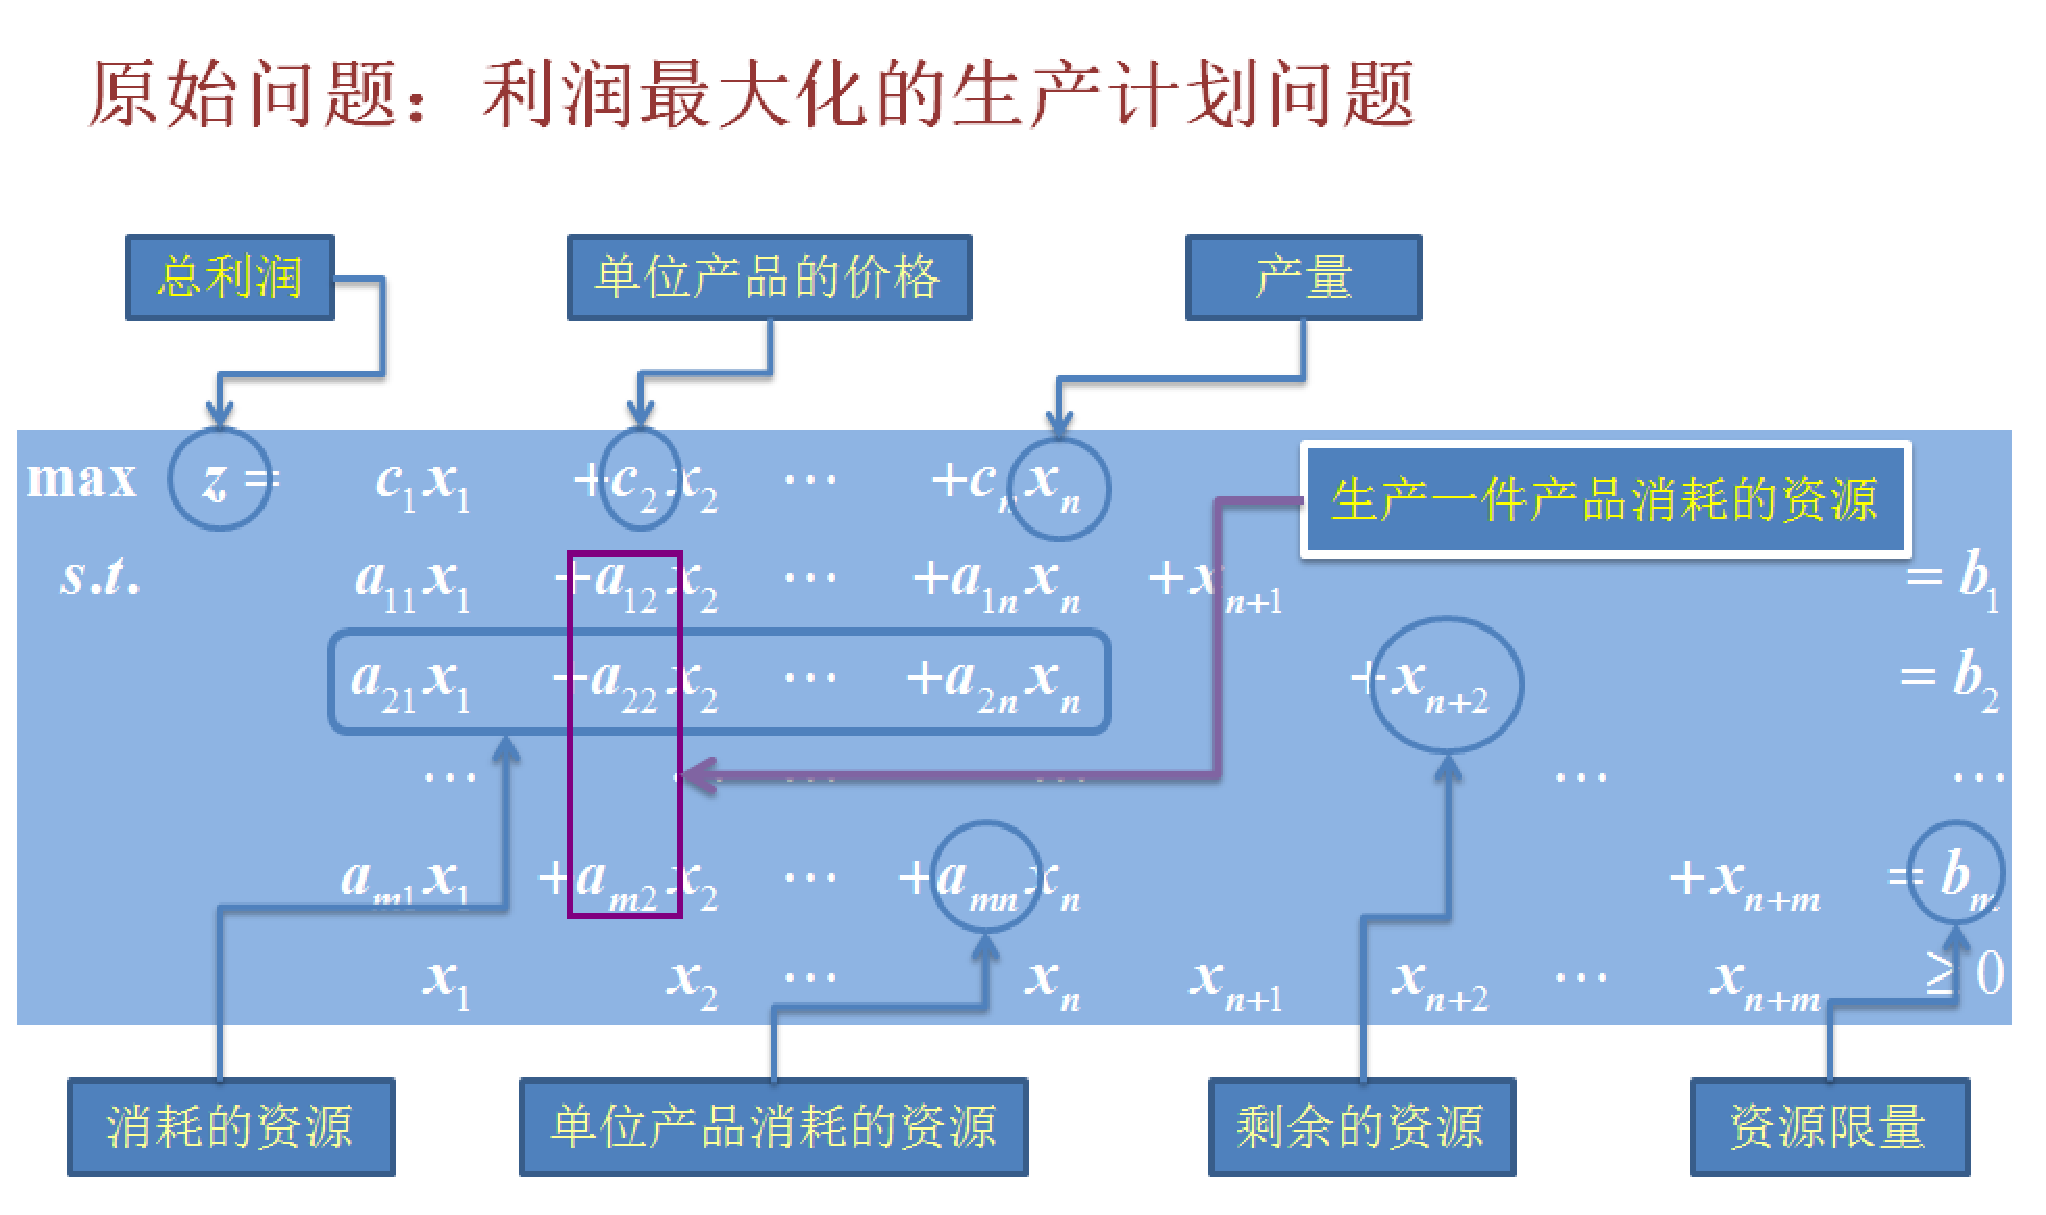
\includegraphics[width=0.9\textwidth]{figures/primal.eps}
\caption{原始问题:利润最大化的生产计划问题}\label{fig:primal}
\end{minipage}
\begin{minipage}[t]{0.49\linewidth}
\centering
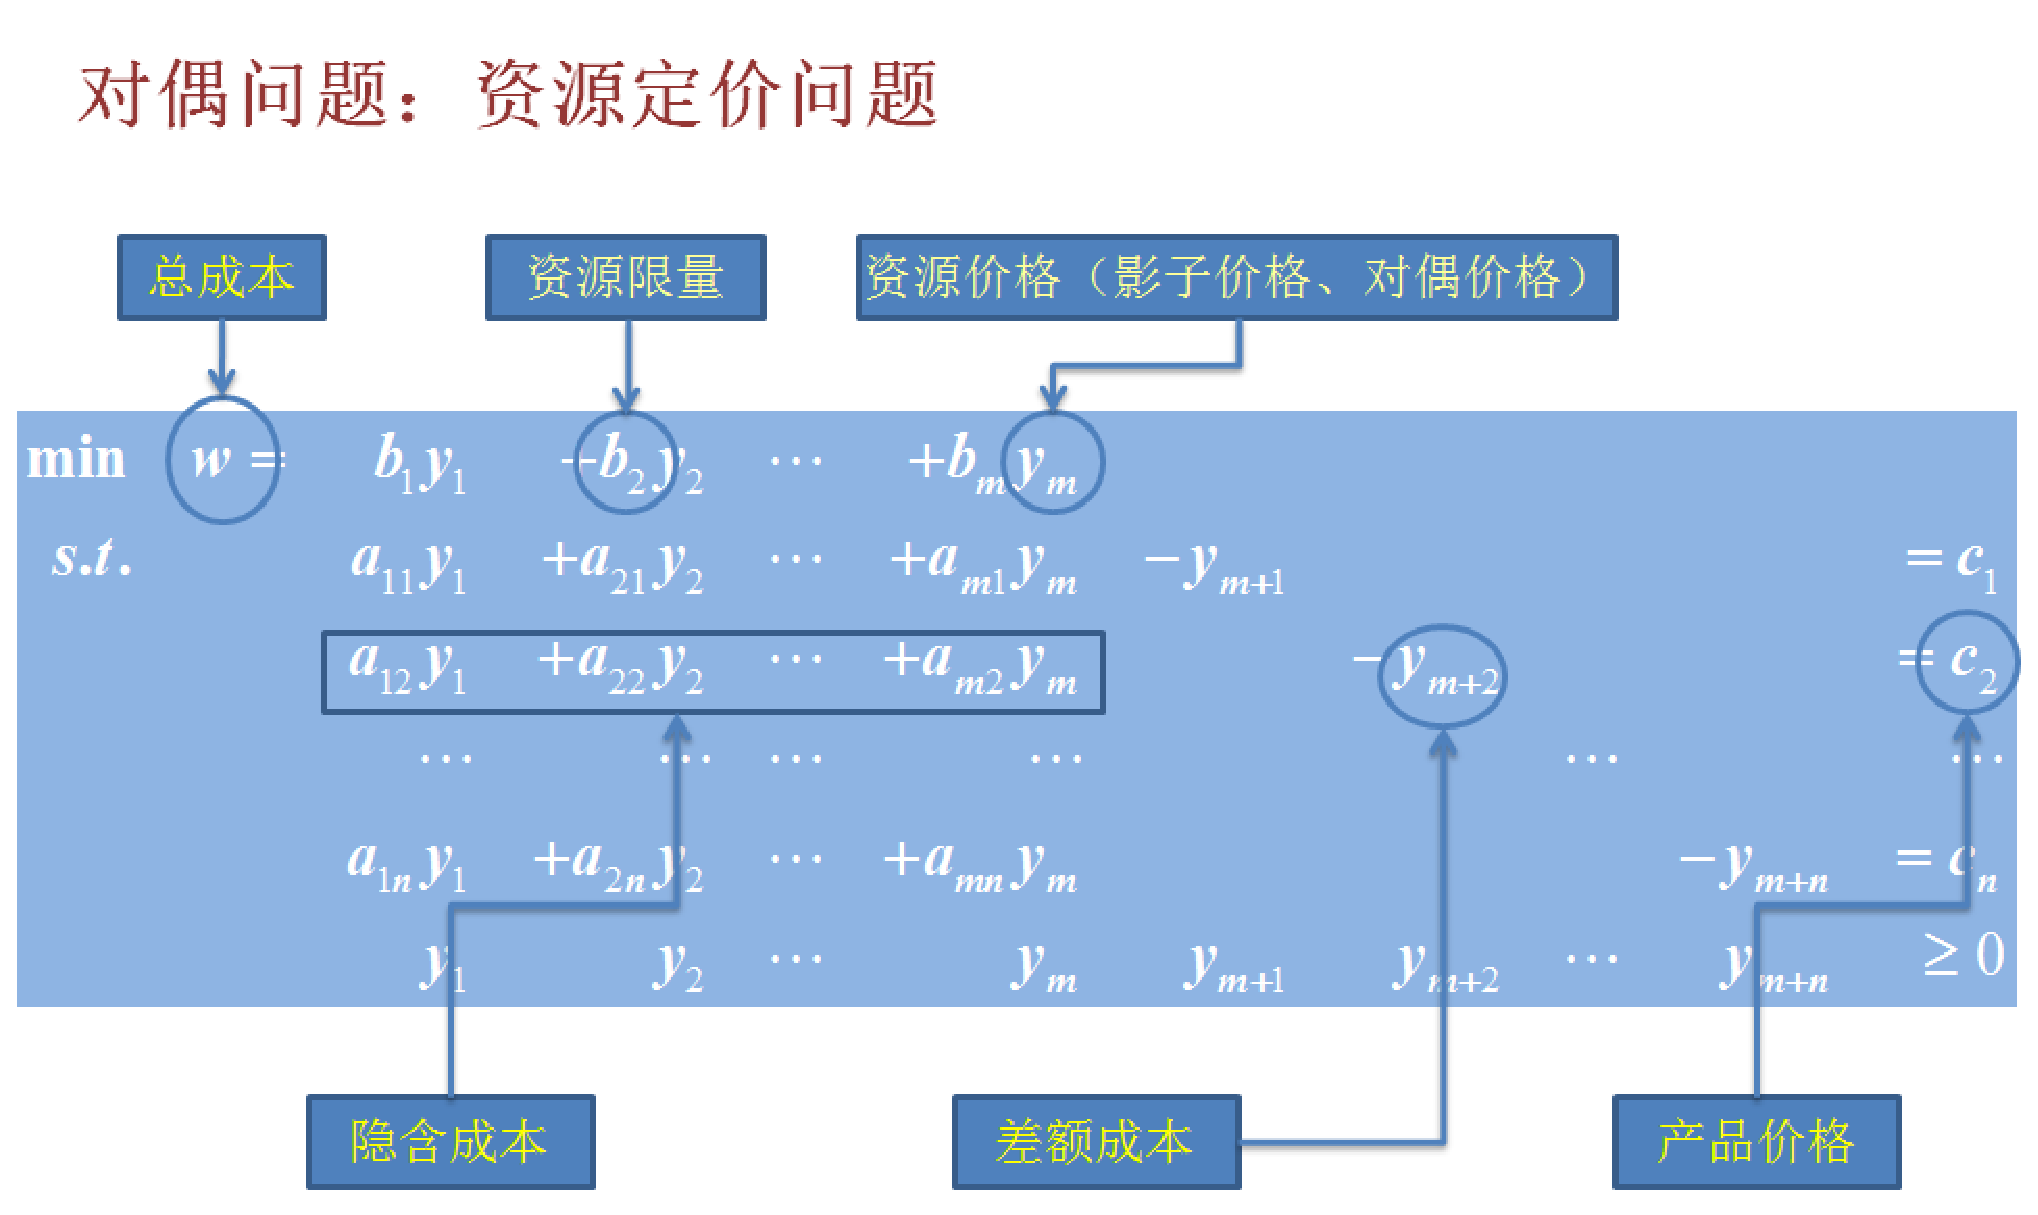
\includegraphics[width=0.9\textwidth]{figures/dual.eps}
\caption{对偶问题:成本最小化的资源定价问题}\label{fig:dual}
\end{minipage}
\end{figure}

在利润最大化的生产计划问题中(见图\ref{fig:primal}),生产一个单位的第2种产品消耗的资源为$a_{12},\ldots, a_{m2}$,各种资源的影子价格由对偶问题\ref{fig:dual} 所反映,即$y_1,y_2,\ldots, y_m$,则生产第2种产品的机会成本(或隐含成本)可以计算:
\begin{equation}\label{eq:oppcost}
  a_{12}y_1 + \ldots + a_{m2}y_m
\end{equation}
如图\ref{fig:dual}所示,根据市场定价,一个单位第2种产品的价格是$c_2$,则生产一个单位某产品的隐含成本1单位该产品的价格之间的差即是差额成本:
\begin{equation}\label{eq:diffcost}
  y_{m+2} = a_{12}y_1 + \ldots + a_{m2}y_m - c_2 = -\sigma_2
\end{equation}

只有当单位产品的市场价格大于隐含成本时,有利可图,(单纯形法中的)检验数($\sigma_2$)为正,始安排生产(进基);否则不安排。如果价格等隐含成本,检验数为0,表明通过生产本产品增加总利润的可能性已不存在(某变量出基后不再进基)。

\section{单纯形法}\label{sec:simplexmethod}
1947年,美国数学家George Dantzig\cite{dantzig1998linear}提出一种解线性规划的迭代算法 -- 单纯形法(Simplex Method),它被评为20世纪十大算法之一。
\footnote{20世纪十大算法包括:Metropolis Algorithm for Monte Carlo\cite{beichl2000metropolis}, Simplex Method for Linear Programming\cite{nash2000dantzig}, Krylov Subspace Iteration Methods\cite{van2000krylov}, The Decompositional Approach to Matrix Computations\cite{stewart2000decompositional}, The Fortran Optimizing Compiler\cite{padua2000fortran}, QR Algorithm for Computing Eigenvalues\cite{parlett2000qr}, Quicksort Algorithm for Sorting\cite{jaja2000perspective}, Fast Fourier Transform\cite{rockmore2000fft}, Integer Relation Detection\cite{bailey2000integer}, Fast Multipole Method\cite{board2000fast}.}

单纯形法在初始表上重复进行初等行变换(Elementary Row Operation,ERO)、高斯消元,由于线性规划方程数目小于变量个数时出现不定解,单纯形法从线性方程组中寻找单纯形,
\footnote{一个$d$维空间$\mathbb{R}^d$中的单纯形$\mathcal{S}$定义为由$d+1$个顶点$x_1,\ldots, x_d\in \mathbb{R}^d$所构成的凸包(Convex Hull)。单纯形就是一种简单的几何形状,通过将$d$ 维空间中的$d+1$个顶点相连形成。比如,一维单纯形是一个边,二维单纯形是一个三角形,三维单纯形就是一个四面体。}
从每一个单纯形中确定一组解,根据单纯形对应的解对目标函数的改变方向,选择下一个单纯形,逐步趋于最值点。

首先考虑如下包含$n$个变量,$m$个约束的标准形式的线性规划问题:
\begin{equation}
  \begin{array}{ll}
  \textit{max} & z = c^Tx\\
  \textit{s.t.} & Ax = b\\
  & x \ge 0
  \end{array}
\end{equation}
其中,$A\in \mathbb{R}^{m\times n}$,一般地,$m\le n$。对于约束条件中包含不等式的情况,可以通过添加松弛变量(Slacks)或剩余变量(Surplus)将其转化为等式形式。

为方便计算,向模型中添加$m$个“人工变量(Artificial Variables)”:
\[
x_{n+i} = b_i - \sum_{j=1}^n{a_{ij}x_j}
\]
则人工变量非负。我们将$x_1,\ldots,x_n$称作非基变量,它们构成的集合记做$\textbf{N}$,$x_{n+1},\ldots,x_{n+m}$称作基变量,它们构成的集合记做$\textbf{B}$。由人工变量的构造可知,非基变量可由基变量线性表出。

在此基础上,可以构建如下形式的规划问题:
\begin{equation}
  \begin{array}{ll}
  \textit{max} & z= \sum\limits_{i\in \textbf{N}}{c_ix_i} \\
  \textit{s.t.} & x_i = b_i - \sum_{j = 1}^n{a_{ij}x_j} ,i\in \textbf{B}\\
  & x \ge 0
  \end{array}
\end{equation}

使用单纯形法求解线性规划问题的基本步骤:
\begin{enumerate}[(1)]
  \item 确定初始基可行解;
  \item 做最优性检验,通过,即是最优解,否则,转入下一步;
  \item 转换可行解,得到相邻的基可行解,转入上一步。
\end{enumerate}

在单纯形法中,原问题的最优解满足:
\begin{enumerate}[(1)]
  \item 是基本解
  \item 可行($X_B = B^{-1}b\ge 0$)
  \item 检验数$C - C_BB^{-1}A\le 0, YA\le C$,即对偶解可行
\end{enumerate}

根据线性规划的基本性质可知,当线性规划方程的数目小于变量个数时,规划问题存在不定解。使用单纯形法解线性规划时,如果线性规划变量个数小于约束条件的个数,则将其转换为对偶问题再求解。

单纯形法易于程序实现,而且容易使用,但是它只适用于可以转化为标准型的规划问题,此外算法迭代次数将随着约束和变量数目的增加而迅速上升。一般地,单纯形法需要$2n-3n$步迭代,其中$n$表示原问题中变量的个数。Karmarkar方法通常仅仅需要迭代次数在$10-100$次即可求解模型,显然在求解大规模问题时更具优势。

\section{内点法}
\textbf{内点法}(Interior Point Method),又称\textbf{牛顿障碍法}(Newton Barrier Method),由John von Neumann提出,后经由Narendra Karmarkar发展成为解线性规划的一个重要方法。

\begin{example}
考虑如下线性规划问题:
\begin{equation}
  \begin{array}{ll}
  \textit{max} & x_1 + x_2 \\
  \textit{s.t.} & 2px_1 + x_2 \le p^2 + 1, p = \{0, 0.1, 0.2, \ldots, 0.9, 1\}\\
  \end{array}
\end{equation}
使用内点法求解它的过程可见图\ref{fig:karmarkar}:
\begin{figure}[htbp]
  \centering
  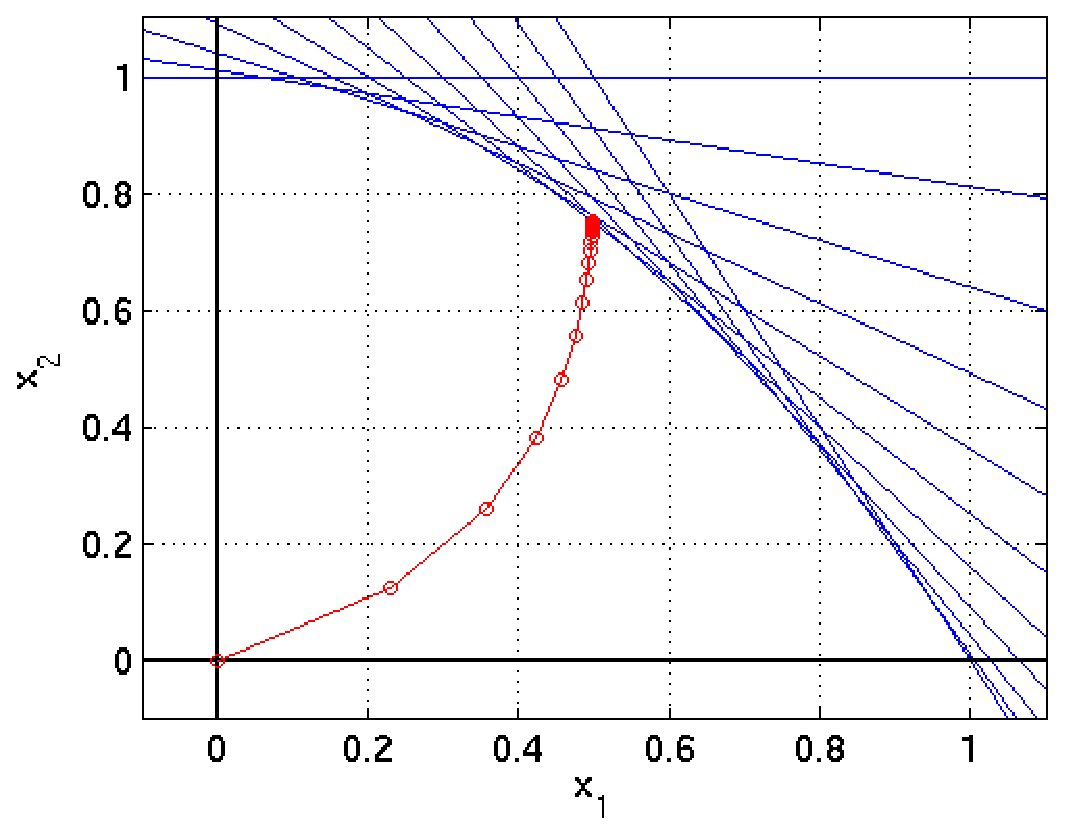
\includegraphics[width=0.6\textwidth, height=8cm]{figures/Karmarkar.eps}\\
  \caption{内点法求解示例}\label{fig:karmarkar}
\end{figure}
图中,蓝色的线表示约束条件,红色线是内点法求解路径。
\end{example}

\section{非线性规划}
在实际应用问题中,无论是问题规模还是变量个数都是庞大的,非线性程度越来越高,难以使用简单的线性模型予以刻画。通常,可以使用目标函数或约束条件至少有一个是非线性函数的数学规划表示,即非线性规划(Nonlinear Programming, NLP),一般可以表示成下面形式:
\begin{equation}\label{eq:nlpproblem}
    \begin{array}{lll}
      \textit{min} & f(x) \\
      \textit{s.t.} & g_i(x) \ge 0, i = 1, \ldots, m\\
       & h_j(x) = 0, j = 1,\ldots, l
    \end{array}
\end{equation}

一般认为,非线性规划诞生的重要标志是1951年Harold W. Kuhn与Albert W. Tucker发表的最优化条件(KT条件)
\cite{karush1939minima,kuhn1951nonlinear}。此后的50 年代主要是对梯度法和牛顿法的研究。在50 年代还发展了可分离规划和二次规划的多种解法,它们大都是以单纯形法为基础。50年代末到60年代末出现了许多解非线性规划问题的有效的算法,70年代又得到进一步的发展。非线性规划在工程、管理、经济、科研、军事等方面都有广泛的应用,为最优设计提供了有力的工具。20世纪80年代以来,计算机的飞速发展使非线性规划的研究如虎添翼,陆续诞生了信赖域法、稀疏拟牛顿法、内点法和有限存储法,在大规模非线性问题求解与并行计算方面也取得长足的发展。

非线性规划数值算法大致可分为\textbf{直接搜索算法}和\textbf{间接搜索算法}。直接搜索算法仅仅利用目标函数值信息直接建立搜索求解的方法,无须借助目标函数的梯度信息,因此又称作无梯度(Non-gradient)算法或零阶(Zeroth Order)算法。直接搜索算法包括随机搜索方法(Random Search)、网格搜索方法(Grid Search)、坐标轮换法(Univariate Search)\cite{desopo1959convex}、旋转坐标法(Rotating Coordinates)\cite{rosenbrock1960automatic}、模式方向法(Pattern Direction)\cite{hooke1961direct}、Powell方法\cite{powell1964efficient}和Nelder-Mead法\cite{nelder1965simplex}。
%遗传算法、差分进化和模拟退火算法
间接搜索算法需要利用一阶导数或黑塞矩阵(Hessian Matrix)信息,故又称为基于梯度的方法,典型的包括最速下降法、共轭梯度法(Fletcher-Reeves)、牛顿法、Marquardt方法、拟牛顿法、序列二次规划方法(Sequential Quadratic Programming, SQP)、增广拉格朗日方法(Augmented Lagrangian Method)和非线性内点法。非线性规划目前还没有适用于各种问题的一般算法,各个方法都有自己特定的适用范围。

%受Ford和Fulkson的关于多货物最大流网络规划问题的启发,1960年Dantzig与Wolfe发明了Dantzig-Wolfe分解原理,开创大规模系统最优化理论之先河,自问世以来在动态投入产出优化模型以为能源规划等许多领域得到广泛应用。

\subsection{基本概念}
由线性规划的性质我们知道,如果\textbf{线性规划}的最优解存在,其最优解只能在其可行域的边界上(特别是可行域的顶点上)达到。\textbf{非线性规划}的最优解(如果存在)则可能在其可行域的任意一点达到。

\begin{definition}[极小值点]
给定集合\textit{S}上的点$\hat x$,如果存在$\varepsilon \ge 0$,对于任意的$x\in $\textit{S},当$\|x-\hat x\| \le \varepsilon$时,都有$f(x) \ge f(\hat x)$,则称$\hat x$是函数$f$在\textit{S}上的\textbf{局部极小值点}。如果对任意的$x \in$ \textit{S},都有$f(x) \ge f(\hat x)$,则$\hat x$是函数$f$在
\textit{S}上的\textbf{全局极小值点}。
\end{definition}

\begin{definition}[驻点、临界点、拐点、鞍点]
如果函数$f$在某点$\hat x$处不可微或$f'(\hat x) = 0$,则称$\hat x$是\textbf{临界点}(Critical Point),对应函数值称作是临界值。如果函数是一阶可导的,且$f'(\hat x) = 0$,则称点$\hat x$ 是\textbf{驻点}(Stationary Point)。如果函数在$\hat x$处由凹变凸或由凸变凹,则称$\hat x$是函数的一个\textbf{拐点}
(Inflection Point),同时如果$f(\hat x)=0$,则称$\hat x$ 是\textbf{鞍点}(Saddle Point)。
\end{definition}

\begin{theorem}[费马定理]
给定函数$f:(a,b) \mapsto \mathbb R$,如果$\hat x\in(a,b)$是$f$的一个局部极值点,若$f$在$\hat x$处是可微的,则$f'(\hat x) = 0$。
\end{theorem}

\begin{definition}[有效约束和无效约束]
假设$x$是非线性规划的一个可行解,它自然满足所有的约束。考虑某不等式约束条件$g_i(x)\ge 0$。当$g_i(x)=0$时,点$x$处于此约束条件形成的可行域边界上,约束条件对点$x$的微小摄动构成限制,则称此约束条件是点$x$的\textbf{有效约束}(active);反之,当$g_i(x)>0$时,约束条件对点$x$的微小摄动(small variation)不会构成限制,则称此约束条件是点$x$的\textbf{无效约束}(inactive)。所有的等式约束条件都是点$x$的有效约束。
\end{definition}

\begin{definition}[可行方向]
假设$x_0$是非线性规划的一个可行解,若存在$\delta>0$,对任意的$\lambda\in (0,\delta)$,$x_0+\lambda d$仍处于可行域上,则称$d$是$x_0$的一个\textbf{可行方向}。
\end{definition}

将$g_i(x)$在点$x_0$处作一阶泰勒展开,由
\[
    g_i(x_0+\lambda d) = g_i(x_0) + \lambda d^T \nabla g_i(x_0) + O(\lambda)
\]
可知满足\textcolor{red}{$d^T \nabla g_i(x_0) \ge 0,i=1,\ldots,m$ 的方向$d$是点$x_0$的一个可行方向}。

\begin{definition}[下降方向]
假设$x_0$是非线性规划的一个可行解,若存在$\delta>0$,对任意的$\lambda\in (0,\delta)$都有$f(x_0+\lambda d)<f(x_0)$,则称$d$是$x_0$的一个\textbf{下降方向}。
\end{definition}

将$f(x)$在点$x_0$处作一阶泰勒展开,由
\[
    f(x_0+\lambda d) = f(x_0) + \lambda d^T \nabla f(x_0) + O(\lambda)
\]
可知满足$d^T \nabla f(x_0) < 0$的方向$d$是点$x_0$的一个下降方向。

\begin{definition}[正则点]
给定某可行解$x$,如果所有有效的不等式约束函数与等式约束函数在$x$处的梯度线性无关,则称点$x$是\textbf{正则点}(Regular Point)。
\end{definition}

根据定义可知,从某点出发,沿任意可行方向(距离很小)都不能使目标函数值减少,则该点即局部极小值点。

\begin{theorem}[最优化的必要性条件]
假设$\hat x$是目标函数$f:\mathbb R^n \mapsto \mathbb{R}$的无约束最小值点,$f$是含$\hat x$的开集\textit{S}上的一阶连续可微函数,则满足\textbf{一阶必要性条件},即$\nabla f(\hat x) = 0$。如果$f$又是二阶连续可微的,则满足\textbf{二阶必要性条件},即$\nabla^2 f(\hat x)$半正定。
\end{theorem}

\section{拉格朗日乘子法}
拉格朗日乘子法(Lagrange Multiplier Method)主要用于解决等式约束的优化问题
\begin{equation}
    \begin{array}{lll}
      \textit{min} & f(x) \\
      \textit{s.t.} & h_i(x) = 0,~~i = 1,\ldots,m
    \end{array}
\end{equation}
其中,$x\in\mathbb{R}^n$,目标函数$f:\mathbb{R}^n \mapsto \mathbb{R}$是一阶连续可微函数。

我们知道,可行域上目标函数$f$的极小值点应当是一个驻点\footnote{Stationary Point:函数在该点处的梯度为零},对于可行域上驻点存在一个有用的性质:
\begin{theorem}
点$x$是可行域上驻点的充要条件是:沿任意可行方向移动点$x$,目标函数值都不会发生改变。
\end{theorem}

给定点$x$,设$V$是保持目标函数值不变的方向集,则从$x$出发不改变目标函数值的任意移动方向皆垂直于目标函数在该点处的梯度。对任意的$v\in V\subset \mathbb{R}^n$,都有等式
\begin{equation}
    v^T \nabla f(x) = 0
\end{equation}
成立。

规划问题中的约束条件限制了点$x$可以移动的方向:同时满足所有的等式约束,不会改变函数$g_i$的值。设$V'$是$x$的可行方向集合,那么从$x$出发不“违背”约束条件的任何移动方向都垂直于约束函数的梯度。对任意的$v\in V'\subset \mathbb{R}^n$,都有等式
\begin{equation}
    v^T \nabla h_i(x) = 0, i = 1,\ldots,m
\end{equation}
成立。我们由此得出结论:
\begin{theorem}
点$x$是可行域上驻点的充要条件是:沿任意方向移动点$x$,如果它改变了目标函数的值,则它至少会违背一个约束条件。
\end{theorem}

假设存在某个从$x$ 出发的移动方向,如果它是可行方向,即满足所有的约束条件,而且在移动后,目标函数值发生改变,无论是变大还是变小,皆表明$x$ 并非可行域上的驻点,矛盾产生。换句话说,目标函数在可行域上驻点$x$处的梯度垂直于由$V'$生成的子集,而后者又与约束函数在$x$处的梯度垂直。

\begin{theorem}[拉格朗日乘子定理]
假设$x^*$是目标函数$f$的局部极小值点,若约束函数的梯度向量组$h_1(x^*),\ldots, h_m(x^*)$\textbf{线性无关}($x^*$是一个正则点),则存在唯一的拉格朗日乘子向量$\Lambda^* = (\lambda_1^*,\ldots,\lambda_m^*)$使得等式
\begin{equation}
    \nabla f(x^*) + \sum\limits_{i=1}^m \lambda_i^* \nabla h_i(x^*) =0
\end{equation}
成立。

如果$f$与$h_i,i=1,\ldots,m$都是二阶连续可微的,则对任意$v\in V(x^*)$
\begin{equation}
    v^T (\nabla^2 f(x^*) + \sum\limits_{i=1}^m \lambda_i^* \nabla^2 h_i(x^*)) v \ge 0
\end{equation}
其中,$V(x^*) = \big\{v\mid v^T \nabla h_i(x^*)=0, i = 1,\ldots,m\big\}$。
\end{theorem}

\begin{proof}
我们下面利用罚函数法(Penalty Approach)给出证明~\cite{bertsekas1999nonlinear}。对于含有等式约束的非线性规划问题,我们通过对违反约束条件的点施加惩罚,将有约束最优化问题转化为无约束最优化问题。为了方便表示,令$h=(h_1,h_2,\ldots,h_m)^T$。

对于$k=1,2,\ldots$,定义函数:
\begin{equation}
    F_k(x) = f(x) + \frac{k}{2} \|h(x)\|^2 + \frac{\alpha}{2} \|x-x^*\|^2
\end{equation}
其中,$x^*$表示约束问题的局部极小值点,$\alpha>0$。第二项是对违反约束条件的点$h(x)=0$施加的惩罚项,第三项则确保$x^*$是
\[
    \begin{array}{ll}
      \textit{min} & f(x) +  \frac{\alpha}{2} \|x-x^*\|^2 \\
      \textit{s.t.} & h(x) = 0
    \end{array}
\]
严格局部极小值点。

由于$x^*$是一个局部极小值点,我们可以选择半径$\varepsilon>0$,使得封闭球
\begin{equation}
    S = \{x\mid \|x-x^*\| \le \varepsilon\}
\end{equation}
内所有可行解$x$,都有$f(x^*) \le f(x)$。

对于约束优化问题
\begin{equation}\label{eq:constainedlagrange}
    \begin{array}{ll}
      \textit{min} & F_k(x) \\
      \textit{s.t.} & x\in S
    \end{array}
\end{equation}
假设其最优解是$x^k$,对于所有的$k$,则有
\begin{equation}\label{neq:bound}
    F_k(x^k) = f(x^k) +  \frac{k}{2} \|h(x^k)\|^2 + \frac{\alpha}{2} \|x^k-x^*\|^2 \le F_k(x^*) = f(x^*)
\end{equation}
由$f(x^k)$在$S$上有界,可知$\lim\limits_{k\rightarrow \infty} h(x^k) = 0$(否则,左端无界,矛盾)。对于每个极限值$\bar{x} = \lim\limits_{k\rightarrow \infty} x^k$,都有$h(\bar{x}) = 0$,从而对不等式~\ref{neq:bound} 两边同时取极限可得:
\begin{equation}
    f(\bar{x}) + \frac{\alpha}{2} \|\bar{x}-x^*\|^2 \le f(x^*)
\end{equation}
由于$\bar{x}\in S$上的可行解,所以$f(x^*) \le f(\bar{x})$,那么$\bar{x} = x^*$,表明当$k$充分大时,$x^k$是$F_k(x)$的无约束局部极小值点。

下面我们利用无约束优化的相关性质证明拉格朗日乘子定理:根据一阶必要条件,当$k$充分大时,有
\begin{equation}\label{eq:lagrangenecessary}
    0 = \nabla F_k(x^k) = \nabla f(x^k) + k \nabla h(x^k) h(x^k) + \alpha (x^k - x^*)
\end{equation}
成立。

由于$\nabla h(x^*)$的秩为$m$,当$k$充分大时$\nabla h(x^k)$有相同的结论,所以$\nabla h(x^k)^T \nabla h(x^k)$ 可逆,那么对于上式,整理可得:
\begin{equation}
    kh(x^k) = -(\nabla h(x^k)^T \nabla h(x^k))^{-1} \nabla h(x^k)^T \big[\nabla f(x^k) + \alpha (x^k - x^*)\big]
\end{equation}
两边同时取极限可知
\begin{equation}
    \lim\limits_{k\rightarrow \infty} kh(x^k) = \Lambda^* = -(\nabla h(x^*)^T \nabla h(x^*))^{-1} \nabla h(x^*)^T \nabla f(x^*)
\end{equation}
根据等式~\eqref{eq:lagrangenecessary}可得
\begin{equation}
    \nabla f(x^*) + \Lambda^* \nabla h(x^*) = 0
\end{equation}
由此证明了一阶优化条件。

对于$F_k(x)$,根据其二阶优化条件可知,当$k$充分大时,对任意的$\alpha>0$,矩阵
\begin{equation}
    \nabla^2 F_k(x^k) = \nabla^2 f(x^k) + k \nabla h(x^k) (\nabla h(x^k))^T + k \sum\limits_{i=1}^m h_i(x^k) \nabla^2 h_i(x^k) + \alpha I
\end{equation}
是半正定的。给定$v\in V(x^*)$,则$v^T \nabla h(x^*) = 0$,取$v^k$表示$v$在$(\nabla h(x^k))^T$零子空间上的投影,则
\begin{equation}
    v^k = v - \nabla h(x^k)\big[(\nabla h(x^k))^T \nabla h(x^k)\big]^{-1} v^T \nabla h(x^k)
\end{equation}
已知$(v^k)^T \nabla h(x^k)=0$,$\nabla^2 F_k(x^k)$半正定,可得
\begin{equation}
    0\le (v^k)^T \nabla^2 F_k(x^k) v^k = (v^k)^T \big[\nabla^2 f(x^k) + k \sum\limits_{i=1}^m h_i(x^k) \nabla^2 h_i(x^k) \big] v^k + \alpha \|v^k\|^2
\end{equation}
由于$x^k\rightarrow x^*$,$kh_i(x^k)\rightarrow \lambda_i^*$,并且$v^T \nabla h(x^*)=0$,则$v^k\rightarrow v$,对任意的$v\in V(x^*)$,都有
\begin{equation}
    0\le v^T \big[\nabla^2 f(x^*) + \sum\limits_{i=1}^m \lambda_i^* \nabla^2 h_i(x^*) \big] v + \alpha \|v\|^2
\end{equation}

参数$\alpha$可以取任意小的正数,则对任意的$v\in V(x^*)$有
\begin{equation}
    0\le v^T \big[\nabla^2 f(x^*) + \sum\limits_{i=1}^m \lambda_i^* \nabla^2 h_i(x^*) \big] v
\end{equation}
证毕。
\end{proof}

根据一阶必要条件和等式约束条件,由$m+n$个方程构建的包含$m+n$ 个未知数的方程组,并确定出唯一解。对于一阶必要条件,要求约束函数的梯度向量组线性无关,如果是线性相关的,那么会产生什么影响呢?我们下面给出一个例子说明这个问题:
\begin{equation}
    \begin{array}{lll}
      \textit{min} & f(x) = x_1 +  x_2 \\
      \textit{s.t.} & h_1(x) = (x_1-1)^2 + x_2^2 - 1 = 0 \\
       & h_2(x) = (x_1-1)^2 + x_2^2 - 4 = 0
    \end{array}
\end{equation}
它只包含一个可行点$(0,0)$,并且是极小值点,两个约束函数的梯度是线性相关的,因此对于任意的$\lambda_1,\lambda_2$,等式
\[
    \nabla f(x^*) + \lambda_1 \nabla h_1(x^*) + \lambda_2 \nabla h_2(x^*) = 0
\]
始终不成立。

\begin{theorem}[充分条件]
假设$f$和$g$是二阶连续可微函数,定义拉格朗日函数
\begin{equation}
    L(x,\Lambda) = f(x) + \Lambda^T h(x)
\end{equation}
设$x^*\in \mathbb{R}^n$,$\Lambda^*\in \mathbb{R}^m$满足
\begin{equation}
    \begin{array}{lll}
      \nabla_x L(x^*,\Lambda^*) & = & 0 \\
      \nabla_{\Lambda} L(x^*,\Lambda^*) & = & 0
    \end{array}
\end{equation}
并且对任意的$v\ne 0$,当$v^T \nabla h(x^*) = 0$时,
\begin{equation}
    v^T \nabla_{xx}^2 L(x^*,\Lambda^*) v > 0
\end{equation}
则$x^*$是非线性等式约束优化问题的严格局部最小值点。
\end{theorem}

充分条件可以使用罚函数法或者可行方向法予以证明~\cite{bertsekas1999nonlinear}。
\subsection{对偶问题与KKT条件}
KKT(Karush-Kuhn-Tucker)条件,又称KT(Kuhn-Tucker)条件,是非线性规划的一个重要结论。早在1939 年,William Karush\cite{karush1939minima} 在其博士论文中就得到这一结论,然而直到Harold W. Kuhn与Albert W. Tucker在1951 年首次公开发表\cite{kuhn1951nonlinear},人们才意识到这一工作的重要性。

KKT条件是对拉格朗日乘子法(Lagrange Multipliers Method)的推广,对于包含不等式约束条件的非线性规划问题:
\begin{equation}\label{eq:nlp}
    \begin{array}{lll}
      \textit{min} & f(x) \\
      \textit{s.t.} & g_i(x) \le 0, i = 1, \ldots, m\\
       & h_j(x) = 0, j = 1,\ldots, l
    \end{array}
\end{equation}
其中,$x\in \mathbb{R}^n$,$f:\mathbb{R}^n \mapsto \mathbb{R}$是目标函数,$g_i:\mathbb{R}^n \mapsto \mathbb{R},(i=1,\ldots,m)$是不等式约束函数,$h_j:\mathbb{R}^n \mapsto \mathbb{R},(j=1,\ldots,l)$是等式约束函数,都是一阶连续可微函数。

构造拉格朗日函数
\begin{equation}
    L(x,\alpha,\beta) = f(x) + \sum\limits_{i=1}^m \alpha_i g_i(x) + \sum\limits_{j=1}^l \beta_j h_j(x)
\end{equation}
其中,$\alpha\ge 0,\beta$为拉格朗日乘子向量。

记$\Theta_p(x) = \max\limits_{\alpha \ge 0,\beta} L(x,\alpha,\beta)$,由于
\begin{equation}
   \max\limits_{\alpha \ge 0,\beta} L(x,\alpha,\beta) =  f(x) + \max\limits_{\alpha \ge 0,\beta} \bigg[\sum\limits_{i=1}^m \alpha_i g_i(x) + \sum\limits_{j=1}^l \beta_j h_j(x) \bigg]
\end{equation}
\begin{itemize}
  \item 当$x$是可行解时,满足所有约束条件,则$h_j(x)=0,j=1,\ldots,l$,函数$\Theta_p(x)$可简化为
  \[
    \Theta_p(x) = f(x) + \max\limits_{\alpha \ge 0,\beta} \sum\limits_{i=1}^m \alpha_i g_i(x)
  \]
  由于$g_i(x)\le 0,i=1,\ldots,m,\alpha \ge 0$,则$\sum\limits_{i=1}^m \alpha_i g_i(x) \le 0$,当且仅当$\alpha=0$时等式成立,从而$\Theta_p(x) = f(x)$。
  \item 当$x$不可行时,违反至少一个约束条件,则通过灵活选择$\alpha,\beta$可得$\Theta_p(x)=\infty$。
\end{itemize}
综上可得
\begin{equation}
    \Theta_p(x) = \max\limits_{\alpha \ge 0,\beta} L(x,\alpha,\beta) = \left\{
        \begin{array}{lll}
          f(x) & x\text{是可行解} \\
          \infty & \text{否则}
        \end{array}
    \right.
\end{equation}
利用拉格朗日函数可以建立如下无约束最优化问题
\begin{equation}\label{eq:lagrangeprimal}
    \hat p = \min\limits_x \Theta_p(x) = \min\limits_x \max\limits_{\alpha\ge 0,\beta} L(x,\alpha,\beta)
\end{equation}
它与原始问题\eqref{eq:nlp}等价(解相同),我们称其为原问题。
如果记$\Theta_d(\alpha,\beta) = \min\limits_x L(x,\alpha,\beta)$,容易证明$\Theta_d(\alpha,\beta) \le \hat p$。假设$x_0$是问题\eqref{eq:lagrangeprimal} 的任意可行解,即$g_i(x_0)\le 0, h_j(x_0)=0, \alpha \ge 0$,则有
\begin{equation}
    \sum\limits_{i=1}^m \alpha_i g_i(x_0) + \sum\limits_{j=1}^l \beta h_j(x_0) \le 0
\end{equation}
从而
\begin{equation}
    L(x_0,\alpha,\beta) = f(x_0) + \sum\limits_{i=1}^m \alpha_i g_i(x_0) + \sum\limits_{j=1}^l \beta h_j(x_0) \le f(x_0)
\end{equation}
也就是说
\begin{equation}
    \Theta_d(\alpha,\beta)= \min\limits_x L(x,\alpha,\beta) \le L(x_0,\alpha,\beta) \le f(x_0)
\end{equation}
由$x_0$的任意性可知,$\Theta_d(\alpha,\beta) \le \hat p$成立。

对于下面形式的问题
\begin{equation}\label{eq:lagrangedual}
    \hat d = \max\limits_{\alpha\ge 0,\beta} \Theta_d(\alpha,\beta) = \max\limits_{\alpha\ge 0,\beta} \min\limits_x L(x,\alpha,\beta)
\end{equation}
构成原问题的对偶问题,必然有
\begin{equation}\label{eq:weakduality}
    \hat d\le \hat p \text{(\textbf{弱对偶性},Weak Duality)}
\end{equation}
差值$\hat p - \hat d$称为\textbf{对偶间隙(Duality Gap)},当对偶间隙为零时
\begin{equation}\label{eq:strongduality}
    \hat d =\hat p \text{(\textbf{强对偶性},Strong Duality)}
\end{equation}

当强对偶性成立时,原问题的最优解是$\hat x$,对偶问题的最优解是$\hat \alpha,\hat\beta$,则拉格朗日函数在可行解$(\hat x,\hat\alpha,\hat\beta)$的函数值同原始问题目标函数值$f(\hat x)$相等,即
\begin{equation}
    L(\hat x,\hat\alpha,\hat\beta) = f(\hat x) + \sum\limits_{i=1}^m \hat\alpha_i g_i(\hat x) + \sum\limits_{j=1}^l \hat\beta_j h_j(\hat x) = f(\hat x)
\end{equation}
\begin{itemize}
  \item $\hat x$是$\Theta_p(x)$的极值点,由拉格朗日函数与$\Theta_p(x)$的定义,极值点的必要条件,可得
    \begin{equation}
        \nabla f(\hat x) + \sum\limits_{i=1}^m \hat\alpha_i \nabla g_i(\hat x) + \sum\limits_{j=1}^l \hat\beta_j \nabla h_j(\hat x) = 0
    \end{equation}
  我们称之为\textbf{平稳性(Stationarity)条件}。
  \item $\hat x$是原始问题的可行解,满足$h_j(\hat x)=0,j=1,\ldots,l$,所以
    \begin{equation}
        \sum\limits_{i=1}^m \hat\alpha_i g_i(\hat x) = 0
    \end{equation}
  既然$\hat\alpha_i g_i(\hat x)\le 0,\forall i$,则有
    \begin{equation}
        \hat\alpha_i g_i(\hat x) = 0, i = 1,\ldots, m
    \end{equation}
  我们称之为\textbf{互补松弛(Complementary Slackness)条件},当$\hat\alpha_i>0$时,必然有$g_i(\hat x)=0$,表明此不等式约束条件是有效的。
\end{itemize}

\subsubsection{必要条件}
如果$\hat x$是极小值点,并且满足一些约束规范条件(Constraint Qualification,Regularity Conditions),则存在拉格朗日乘子向量$\hat \alpha \in \mathbb{R}^m,\beta\in \mathbb{R}^l$,满足下面几条性质(统称为KKT优化条件):
\begin{itemize}
  \item \textbf{主可行性条件}(Primal Feasibility Conditions)
  \begin{equation}
    \begin{array}{ccc}
      g_i(\hat x) & \le & 0 \\
      h_j(\hat x) & = & 0
    \end{array}
  \end{equation}
  \item \textbf{对偶可行性条件}(Dual Feasibility Condition)
  \begin{equation}
    \hat\alpha_i \ge 0
  \end{equation}
  \item \textbf{互补松弛条件}
  \begin{equation}
    \hat\alpha_i g_i(\hat x) = 0
  \end{equation}
  \item \textbf{平稳性条件}
  \begin{equation}
    \nabla f(\hat x) + \sum\limits_{i=1}^m \hat\alpha_i \nabla g_i(\hat x) + \sum\limits_{j=1}^l \hat\beta_j \nabla h_j(\hat x)=0
  \end{equation}
\end{itemize}
其中,$i = 1, \ldots, m, j = 1,\ldots, l$。特别地,当$m=0$时,非线性规划仅含等式约束,则KTT条件退化为拉格朗日条件。

\subsubsection{约束规范条件}
对于极值点$\hat x$,若满足KKT必要性条件,必需满足一些约束规范条件。常用的约束规范条件有
\begin{itemize}
  \item 线性无关约束规范条件(Linear Independence Constraint Qualification, LICQ):有效不等式约束函数与等式约束函数在$\hat x$处的梯度线性无关(正则点)
  \item Slater约束规范条件:对于凸优化问题,所有的有效不等式约束在点$\hat x$处是严格不等式
\end{itemize}

\subsubsection{充分条件}
假设目标函数$f$与不等式约束函数$g_i(i=1,\ldots,m)$都是凸函数,等式约束函数$h_j(j=1,\ldots,l)$是仿射函数,$\hat x$是一个可行解,如果存在$0\le \hat\alpha \in \mathbb{R}^m,\beta\in \mathbb{R}^l$,满足\textbf{互补松弛}与\textbf{平稳性}条件,则$\hat x$是\textbf{全局极小值点}。

\subsubsection{Fritz John必要条件}
对于非线性优化问题
\begin{equation}
    \begin{array}{lll}
      \textit{min} & f(x) \\
      \textit{s.t.} & g_i(x) \le 0, i = 1, \ldots, m\\
    \end{array}
\end{equation}
根据Farkas引理,设$\hat x$是一个局部极小值点,则存在不全为零的拉格朗日乘子$\hat \lambda_i,i=0,1,\ldots,m$,满足下面几个性质(统称Fritz John必要条件)
\begin{equation}\label{eq:fritzjohn}
    \begin{array}{rcl}
      \hat \lambda_0 \nabla f(\hat x) + \sum\limits_{i=1}^m \hat\lambda_i \nabla g_i(\hat x) &=& 0 \\
      \hat \lambda_i &\ge& 0,~~i = 0,1,\ldots,m \\
      \hat \lambda_i g_i(\hat x) &=& 0,~~i = 1,2,\ldots,m
    \end{array}
\end{equation}

当原问题比较复杂,而对偶问题具有良好的结构时,利用原问题的强对偶性“通过求解对偶问题实现对原问题的求解”是一种常用的优化方法,比如当目标函数与不等式约束函数都是凸函数,等式约束函数是仿射函数,而不等式约束条件是严格的,则相应的优化问题是强对偶的。一般而言,KKT条件是强对偶性成立的必要条件,特别地,当原问题是凸优化问题时,KKT条件是强对偶性成立的充分必要条件。

\section{梯度下降法}
\textbf{梯度下降法}(Gradient Descent Method),又称\textbf{最速下降法}(Steepest Descent Method),由大数学家Cauchy于1847年最先使用。它是最古老的一种解析方法,而其他解析方法大多承其衣钵,并构成最优化方法的基础。梯度下降法的优点是工作量少,存储变量少,对初始点不敏感。当然,它也有缺点。比如,对于多峰形式(Multi-Modal)的参数分布,它的收敛速度很慢,容易陷入局部最优点。

如果我们希望利用迭代算法寻找二阶可微函数$f$的最小点,假设当前最优点是$x_k\in \mathbb{R}^n$,在选择下一个点 $x_{k+1} = x_k + \alpha h$ 时,遵循的原则或目标是能够最小化函数值
$f(x_{k+1})$,即
\begin{equation}\label{eq:gradientdescent}
    \begin{array}{ll}
        \min\limits_{h \in \mathbb{R}^n} & f(x_{k+1}) = f(x_k + \alpha h)
    \end{array}
\end{equation}
其中,$h$表示搜索的方向,一般地$\|h\| = 1$,$\alpha>0$表示步长或者学习率(Learning Rate)。

根据泰勒展开公式有:
\[
    f(x_k + \alpha h) = f(x_k) + \alpha g(x_k)^T h + O(\alpha)
\]
其中,$g(x_k) = \nabla f(x_k)$。

不考虑高阶部分,等式\eqref{eq:gradientdescent}等价于最小化$g(x_k)^T h$。根据内积公式可知,当$h = -g(x_k) = -\nabla f(x_k)$ (负梯度方向)时,$f(x_k)$下降的速度最快(最速下降法由此而来)。

梯度下降法在机器学习中有广泛的应用,比如在监督型学习算法中,根据经验风险最小化原则训练模型就可能用到梯度下降法。假设预测模型一阶可微$f=f(\omega,x)$,则预测模型在数据集$S=\{x_i,y_i\}_{i=1}^n$上的经验损失
\begin{equation}
    L(\omega,S) = \frac{1}{n} \sum\limits_{i=1}^n \ell(y_i,f(\omega,x_i))
\end{equation}
其中,$\ell(y,f(\omega,x))$是预测模型在单个样本上的损失函数,假设它是一阶可微的。

根据梯度下降法有下面的参数更新法则有:
\begin{equation}
    \omega_{t+1} = \omega_t + \alpha \frac{1}{n} \sum\limits_{i=1}^n \nabla L(y_i, f(\omega,x_i))
\end{equation}
由于每次更新模型参数时,都要用到所有的训练样本,梯度下降法也称\textbf{批量梯度下降法}。批量梯度下降法在更新参数时,用到了数据集中全部的样本,时间复杂度为$O(n)$。

在大数据处理时,对于某些类型的损失函数,计算所有样本的平均梯度值是不可行的。为此,研究人员提议使用随机抽取的单个样本计算近似的平均梯度值,利用它来更新模型参数,能够在大幅减少单次迭代计算量的同时,还能取得同批量梯度下降法相似的效果,这种方法被称作\textbf{随机梯度下降法},也称\textbf{增量随机梯度下降法}。

假设随机选取的样本是$x_0$,则使用下面的公式更新参数:
\begin{equation}
    \omega_{t+1} = \omega_t + \alpha_t \nabla L(y_0, f(\omega,x_0))
\end{equation}
为保证收敛,通常要求学习率$\alpha_t$序列满足
\begin{equation}
    \sum\limits_{t=1}^T \alpha_t = \infty,~~\sum\limits_{t=1}^T \alpha_t^2 < \infty
\end{equation}
一般选择$\alpha_t=1/t$或$\alpha_t=\alpha_0(1+\lambda\alpha_0)^{-1}$。

随机梯度下降法由于单次迭代计算量小,效率很高,远优于经典的优化算法,如牛顿法,特别适合大数据机器学习\cite{bottou2010large}。它也存在一些缺陷,比如在迭代过程中产生许多噪声、每次迭代的搜索方向未必是整体梯度下降的方向等。随机梯度下降法已经被用于训练线性的支持向量机
\cite{shalev2011pegasos}、 条件随机场模型\cite{vishwanathan2006accelerated}。

1992年,Polyak与Juditsky\cite{polyak1992acceleration}在随机梯度下降法的基础上,每次更新参数时,增加一个计算参数平均值的过程
\begin{equation}
    \bar{\omega}_{t+1} = \frac{t}{t+1} \bar{\omega}_t + \frac{1}{t+1} \omega_{t+1}
\end{equation}
并使用收敛的参数平均值作为最优参数,因此称为\textbf{平均随机梯度下降法}(Averaged Stochastic Gradient, ASGD)。平均随机梯度下降法的优点是实现简单,无需计算目标函数Hessian 矩阵逆的情况下,就可以达到与二阶随机梯度下降法相似的渐进收敛速度,比随机梯度下降法还快。然而,在实际应用中,平均随机梯度下降法却遭受冷遇\cite{xu2011towards,lin2011large},部分原因在于其渐进收敛速度要求训练集足够大,在中小型训练集上的表现逊色于随机梯度下降法,部分原因是对于参数调优的要求较高。2010年,Wei Xu\cite{xu2011towards}设计了一套新的学习率调整规则(Learning Rate Schedule)
\begin{equation}
    \alpha_t = \alpha_0 (1+\gamma\alpha_0)^{-c}
\end{equation}
扩大了平均随机梯度下降法的适用范围,使平均随机梯度下降法逐渐被接受和使用,比如Lin等人\cite{lin2011large}设计了一种并行随机梯度下降法,求解线性支持向量分类模型,做大规模图片分类。通常,$\alpha_0$ 选择的数值很小(比如$\alpha_0=0.01$)。参数$\gamma$、$c$ 的选取则需要具体问题具体分析。对于$\gamma$,\cite{xu2011towards}分析认为最好选择使用目标函数Hessian矩阵的最小特征值;对于$c$,常见的选择有$\{1,3/4,2/3\}$。

\subsection{共轭梯度下降法}
共轭梯度下降法(Conjugate Gradient Descent Method)是一种共轭方向法,我们首先熟悉一下共轭与共轭方向的含义。
\begin{definition}[共轭]
假设$A\in \mathbb{R}^{n\times n}$是一个对称正定矩阵,如果存在两个向量$x,y\in \mathbb{R}^n$,使得
\begin{equation}\label{eq:conjugatedirection1}
    x^T A y = 0,
\end{equation}
我们称$x$和$y$关于矩阵$A$\textbf{共轭}。如果$A$是单位矩阵,则$x^T y = 0$,即$x,y$正交,可知正交是共轭的一个特例。
\end{definition}

\begin{definition}[共轭方向]
如果存在一组非零向量$\{x_k\}_{k=1}^n$,对任意两个向量$x_i,x_j$都有
\begin{equation}\label{eq:conjugatedirection2}
    x_i^T A x_j = 0,
\end{equation}
我们称向量族$\{x_k\}_{k=1}^n$关于矩阵$A$共轭,每个向量对应一个\textbf{共轭方向}。
\end{definition}

共轭方向在寻找二次型函数$f(x) = c + b^T x + \frac{1}{2} x^T A x$ 极小值点时,存在一个重要的性质:从任意初始点出发,依次沿$x_1,x_2,\ldots, x_n$方向做一维最优搜索,至多$n$步即可收敛到极小值点。共轭方向法有限步收敛的性质,因此可以称作是二次收敛算法。

理论与实践证明,将二次收敛算法用于非二次型目标函数,亦有很好的效果,但不能保证经过有限次迭代达到极小点。此时,可以对目标函数在极小点附近进行泰勒展开,略去二次项之后的高阶项对目标函数做二次逼近。

\subsection{坐标下降法}
坐标下降法(Coordinate Descent Method)是一种非梯度优化算法,用于寻找一个多元函数的极值点。坐标下降法在每次迭代过程,基于当前点沿某个坐标方向进行一维搜索,并在后续优化过程循环使用不同的坐标方向。

给定某多元函数
\[
    f:\mathbb R^n \mapsto \mathbb R
\]
搜索空间的坐标基是$e_1,\ldots,e_n$,当前所在的点是$x^t=(x_1^t,\ldots,x_n^t)$。假设下一次搜索选择的方向是$e_i$,坐标下降法则固定其他坐标方向上的数值,在方向$e_i$做一维搜索,以优化目标函数:
\begin{equation}
    x_i^{t+1} = \argmin\limits_{x} F(x) = f(x_1^t,\ldots,x_{i-1}^t,x,x_{i+1}^t,\ldots,x_n^t)
\end{equation}

坐标下降法可以归结为下面的简单流程:
\begin{algorithm}[htbp]
        \caption{坐标下降法}
        \begin{algorithmic}
            \REQUIRE ~~初始点$x^0$,偏差阈值$\epsilon_0>0$\\
            \FOR{$k = 1,2,\ldots$}
            \STATE
            \begin{enumerate}
                \item 选择坐标方向$e_1$进行一维搜索
                \[
                    x_1^k = \argmin\limits_{x_1} f(x_1,x_2^{k-1},\ldots,x_n^{k-1})
                \]
                \item 将$x_1^k$代入函数,选择坐标方向$e_2$进行一维搜索
                \[
                    x_2^k = \argmin\limits_{x_2} f(x_1^k,x_2,x_3^{k-1},\ldots,x_n^{k-1})
                \]
                \item 将$x_2^k$代入函数,选择坐标方向$e_2$进行一维搜索
                \[
                    x_3^k = \argmin\limits_{x_3} f(x_1^k,x_2^k,x_3,x_4^{k-1},\ldots,x_n^{k-1})
                \]
                \item 依照上步方式依次做下一个坐标方向上的搜索,直至在所有坐标方向上执行一遍,得到新的搜索点
                \[
                    x^k = (x_1^k,x_2^k,\ldots,x_n^k)
                \]
                \item 计算偏差$\epsilon=|f(x^{k-1}) - f(x^k)|$,如果$\epsilon<\epsilon_0$,则停止迭代,否则重复上述步骤。
            \end{enumerate}
            \ENDFOR
        \end{algorithmic}
\end{algorithm}

\subsection{次梯度法}
二十世纪八十年代,Naum Shor\cite{shor1985minimization,shor2012minimization}研究发明了\textbf{次梯度法}(Subgradient Method),它是解凸优化问题的一种迭代算法,也适用于目标函数不可微的情形。当目标函数可微时,其搜索方向同最速下降法相同。从速度上来看,次梯度法比牛顿法略逊一筹,但是由于它内存消耗少,适合处理大型问题。

\section{牛顿法}
梯度法在某些情况下收敛速度会很慢,无法有效地确定最优搜索方向。如果在梯度法所使用的一阶偏导信息外,我们利用其他更多信息,比如目标函数的二阶偏导,则可以有效改善梯度法,高效地确定最优搜索方向,此法称作\textbf{牛顿法}(Newton's Method)或\textbf{牛顿-拉弗森法}(Newton-Raphson Method)
\footnote{牛顿法最初由艾萨克$\cdot$牛顿发明,后于1690年由约瑟夫$\cdot$拉弗森再次提出。}。

假设目标函数$f(x)$在点$x=x_k$有定义并且连续,则我们可以在此处做二阶泰勒展开,从而有
\[
    f(x) = f(x_k) + (\nabla f(x_k))^T (x - x_k) + \frac{1}{2} (x - x_k)^T (\nabla^2 f(x_k)) (x - x_k)  + O((x - x_k)^2).
\]

为了搜索到目标函数的最小值点,我们使用迭代算法思想,从当前点$x=x_k$出发,搜索下一个最优点$x=x_{k+1}$,使得目标函数值不断下降。如果迭代算法先后两次优化结果数值上比较接近,则可以忽略高阶项$O((x - x_k)^2)$,并得到目标函数的近似表达式
\begin{equation}
    f(x) \approx f(x_k) + (\nabla f(x_k))^T (x - x_k) + \frac{1}{2} (x - x_k)^T (\nabla^2 f(x_k)) (x - x_k).
\end{equation}
根据连续函数极值条件可得$\nabla f(x) = \nabla f(x_k) + \nabla^2 f(x_k) (x - x_k) = 0$。
如果黑塞矩阵$\nabla^2 f(x_k)$可逆,可以直接推得最优搜索路径:
\begin{equation}
    x_{k+1} = x_k - (\nabla^2 f(x_k))^{-1} (\nabla f(x_{k+1}) - \nabla f(x_k)).
\end{equation}
如果黑塞矩阵是奇异矩阵,需要对算法进行修正。由于牛顿法利用目标函数的二阶偏导信息修正搜索方向,收敛速度很快。同时,牛顿法在处理黑塞矩阵,特别是计算黑塞矩阵的逆矩阵时,会产生大量的计算开销。牛顿法利用二阶泰勒展开式逼近目标函数,如果$f(x)$对应一个二次函数,可以直接确定最优解析解。多数情况下,目标函数不属于二次函数,由于泰勒展开存在逼近误差,算法不可能直接搜索到最优值点。当目标函数属于高次函数时,优化速度会受到很大影响。

\begin{shaded}
\noindent 假设目标函数$f(x)$二阶可微,则函数的一阶偏导,又称\textbf{梯度向量},形式如下:
\begin{equation}
g(x)=\nabla f=(\frac{\partial f}{\partial x_1},\frac{\partial f}{\partial x_2},\ldots, \frac{\partial f}{\partial x_n})^T.
\end{equation}
函数的二阶偏导矩阵,又称\textbf{黑塞矩阵}(Hessian Matrix),形式如下:
\begin{equation}\label{eq:hessianmatrix}
    H(x)=\nabla^2 f =
    \begin{bmatrix}
    \partial^2 f/\partial x_1^2 & \cdots & \partial^2 f/\partial x_1\partial x_n \\
    \vdots & \ddots & \vdots \\
    \partial^2 f/\partial x_n\partial x_1 & \cdots & \partial^2 f/\partial x_n^2
    \end{bmatrix}=H^T(x)
\end{equation}
黑塞矩阵$H(x)$亦称为梯度向量$g(x)$的\textbf{雅克比矩阵}(Jacobian Matrix)。
\end{shaded}

\section{拟牛顿法}
1959年,物理学家William C. Davidon\cite{davidon1991variable}设计提出拟牛顿法(Quasi-Newton Methods),也称变尺度法(Variable Metric Method),以解决非线性优化问题。根据牛顿法最优搜索路径:$x_{k+1} - x_k = (\nabla^2 f(x_k))^{-1} (\nabla f(x_{k+1}) - \nabla f(x_k))$,黑塞矩阵反映了目标函数的二阶信息,有利于加快算法的迭代速度,但计算黑塞矩阵逆矩阵的运算却十分复杂。William Davidon\cite{davidon1991variable}设计出一种新的算法,既能够利用目标函数的二阶信息,还能避免直接进行逆矩阵运算:\textbf{通过构造新的矩阵,逼近黑塞矩阵的逆矩阵}。矩阵近似逼近的策略是拟牛顿算法的核心思想,并以此衍生出多种形式的优化算法,如DFP更新方程\cite{fletcher1963rapidly}(DFP Updating Formula)、BHHH方法SR1方程(Symmetric Rank One)、BFGS法与L-BFGS(Limited-memory BFGS)\cite{broyden1967quasi,fletcher1970new,goldfarb1970family,shanno1970conditioning}等高效的优化方法。

拟牛顿法使用$\bar{H}_{k+1}$表示黑塞矩阵逆矩阵$[\nabla^2 f(x_k)]^{-1}$的近似矩阵,每一步迭代都充分利用当前信息确定下一个搜索方向,确保目标函数值随迭代次数增加而稳步下降,近似矩阵最终将收敛于最优解对应的黑塞矩阵的逆。对于目标函数$f(x)$,拟牛顿法根据下面形式的搜索规则
\begin{equation}\label{eq:qnm}
    x_{k+1} - x_k = \bar{H}_{k+1} (\nabla f(x_{k+1}) - \nabla f(x_k))
\end{equation}
实现高效搜索。为方便表示,我们记
\begin{equation}
    \left\{
        \begin{array}{l}
          \Delta x_k = x_{k+1} - x_k \\
          \Delta G_k = \nabla f(x_{k+1}) - \nabla f(x_k)
        \end{array}
    \right.
\end{equation}
则拟牛顿法的搜索路径可以简单写作:
\begin{equation}
    \Delta x_k = \bar{H}_{k+1} \Delta G_k.
\end{equation}

假设近似矩阵$\bar{H}_{k+1}$(\textbf{尺度矩阵})有下面形式的结构
\begin{equation}
    \bar{H}_{k+1} = \bar{H}_k + \Delta \bar{H}_k,
\end{equation}
在上次迭代的近似矩阵$\bar{H}_k$基础上进行调整,$\Delta \bar{H}_k$即校正矩阵。一般地,算法要求近似矩阵为对称正定矩阵,则校正矩阵也是对称矩阵。如果将拆分形式的近似矩阵$\bar{H}_{k+1}$代入\eqref{eq:qnm}可得:
\begin{equation}
    \Delta x_k = (\bar{H}_k + \Delta \bar{H}_k) \Delta G_k = \bar{H}_k \Delta G_k + \Delta \bar{H}_k \Delta G_k.
\end{equation}
此时,我们的目标就是构造合适的校正矩阵,以满足:
\begin{equation}
    \Delta \bar{H}_k \Delta G_k = \textcolor{red}{\Delta x_k} - \textcolor{blue}{\bar{H}_k \Delta G_k}.
\end{equation}

由于校正矩阵是对称矩阵,我们利用两个列向量$\Delta x_k$与$\Delta G_k$,构造如下形式的校正矩阵
可以设想,$\Delta \bar{H}_k$存在一种简单的形式:
\begin{equation}
    \Delta \bar{H}_k = \textcolor{red}{\Delta x_k} (\eta_k \textcolor{red}{\Delta x_k})^T - \textcolor{blue}{\bar{H}_k \Delta G_k} (\xi_k \textcolor{blue}{\bar{H}_k \Delta G_k})^T.
\end{equation}
等式左右两端同时乘以$\Delta G_k$,则有:
\begin{equation}
    \begin{array}{lll}
      \Delta \bar{H}_k \Delta G_k & = & \Delta x_k \textcolor{red}{(\eta_k \Delta x_k)^T \Delta G_k} - \bar{H}_k \Delta G_k \textcolor{red}{(\xi_k \bar{H}_k \Delta G_k)^T \Delta G_k} \\
       & = & \Delta x_k - \bar{H}_k \Delta G_k
    \end{array}
\end{equation}
根据对应关系,我们可以取
\begin{equation}
\left\{
    \begin{array}{lll}
        (\eta_k \Delta x_k)^T \Delta G_k  & = & 1 \\
        (\xi_k \bar{H}_k \Delta G_k)^T \Delta G_k & = & 1
    \end{array}
\right.
\end{equation}
如果$(\Delta x_k)^T \Delta G_k$,$(\bar{H}_k \Delta G_k)^T \Delta G_k$都不等于零,我们可以立即确定两个待定参数
\begin{equation}
    \left\{
        \begin{array}{lll}
          \eta_k & = & 1/(\Delta x_k)^T \Delta G_k \\
          \xi_k & = & 1/(\bar{H}_k \Delta G_k)^T \Delta G_k
        \end{array}
    \right.
\end{equation}
从而得到校正矩阵
\begin{equation}
    \Delta \bar{H}_k = \frac{\Delta x_k (\Delta x_k)^T}{(\Delta x_k)^T \Delta G_k} - \frac{(\bar{H}_k \Delta G_k) (\bar{H}_k \Delta G_k)^T }{(\bar{H}_k \Delta G_k)^T \Delta G_k}
\end{equation}
及尺度矩阵
\begin{equation}\label{eq:scalematrix}
    \bar{H}_{k+1} = \bar{H}_k + \frac{\Delta x_k (\Delta x_k)^T}{(\Delta x_k)^T \Delta G_k} - \frac{(\bar{H}_k \Delta G_k) (\bar{H}_k \Delta G_k)^T }{(\bar{H}_k \Delta G_k)^T \Delta G_k}.
\end{equation}
迭代时常取第一个尺度矩阵$\bar{H}_0$为单位矩阵。

\begin{theorem}
如果$x_k$不是目标函数$f(x)$的极小值点,且$\bar{H}_k$是正定矩阵,则有
\[
    (\Delta x_k)^T \Delta G_k \ne 0, ~~~(\bar{H}_k \Delta G_k)^T \Delta G_k\ne 0,
\]
根据式子\eqref{eq:scalematrix}构造尺度矩阵。如果$\bar{H}_k$是对称正定矩阵,则根据式子\eqref{eq:scalematrix}确定的尺度矩阵$\bar{H}_{k+1}$也是对称正定矩阵。拟牛顿法确定的搜索方向是\textbf{梯度下降方向}。
\end{theorem}

\subsection{DFP变尺度法}
拟牛顿法以较小的代价构造黑塞矩阵的近似矩阵,不要求黑塞矩阵的近似矩阵是非奇异矩阵(可逆),能够产生超线性收敛性,性能优于牛顿法与梯度法。根据拟牛顿法思想,Roger Fletcher与Michael Powell\cite{fletcher1963rapidly}发展出\textbf{DFP变尺度法}(Davidon-Fletcher-Powell Variable Metric Method)。
\begin{algorithm}[htbp]
        \caption{DFP变尺度法}
        \begin{algorithmic}
            \REQUIRE ~~初始点$x_0$,梯度偏差阈值$\epsilon>0$,初始尺度矩阵$\bar{H}_0 = I$(单位矩阵)\\
            \FOR{$k = 1,2,\ldots$}
            \STATE
            \begin{enumerate}
                \item 如果梯度偏差$\|\nabla f(x_k) - \nabla f(x_{k-1})\| \le \epsilon$,则认定$x_{k-1}$是近似极小值点,停止迭代。否则,转向下一步。
                \item 计算尺度矩阵
                    \[
                        \bar{H}_k = \bar{H}_{k-1} + \frac{\Delta x_{k-1} (\Delta x_{k-1})^T}{(\Delta x_{k-1})^T \Delta G_{k-1}} - \frac{(\bar{H}_{k-1} \Delta G_{k-1}) (\bar{H}_{k-1} \Delta G_{k-1})^T }{(\bar{H}_{k-1} \Delta G_{k-1})^T \Delta G_{k-1}}
                    \]
                \item 取搜索方向$d_k = -\bar{H}_k (\nabla f(x_k) - \nabla f(x_{k-1}))$,并在$d_k$方向上进行一维搜索,确定最佳步长$\lambda_k$:
                    \[
                        \lambda_k = \argmin\limits_{\lambda>0} f(x_k + \lambda d_k)
                    \]
                \item 确定下一个搜索点$x_{k+1} = x_k + \lambda_k d_k$
            \end{enumerate}
            \ENDFOR
        \end{algorithmic}
\end{algorithm}

\subsection{BFGS}
BFGS(Broyden-Fletcher-Goldfarb-Shanno)算法是CG Broyden\cite{broyden1967quasi}、Roger Fletcher\cite{fletcher1970new}、Donald Goldfarb\cite{goldfarb1970family}、David Shanno\cite{shanno1970conditioning} 各自独立提出的一种拟牛顿法,它是目前最流行的也是最有效的一种校正方法。BFGS 是DFP 法的对偶形式,在处理非平滑优化问题时,BFGS也能够取得很好的性能。它还存在一个变体,有限内存的BFGS 算法(Limited-memory BFGS, L-BFGS),实现占用的内存远小于BFGS 算法。BFGS 在计算过程中,需要存储一个$n\times n$的矩阵$H$。对于高维矩阵,如$n=100,000$,若使用双精度类型存储矩阵$H$,占用内存$100,000\times 100,000 \times 8$B$\approx 74.5$GB,因此L-BFGS在实际应用中的意义显而易见。
\begin{figure}[htbp]
  \centering
  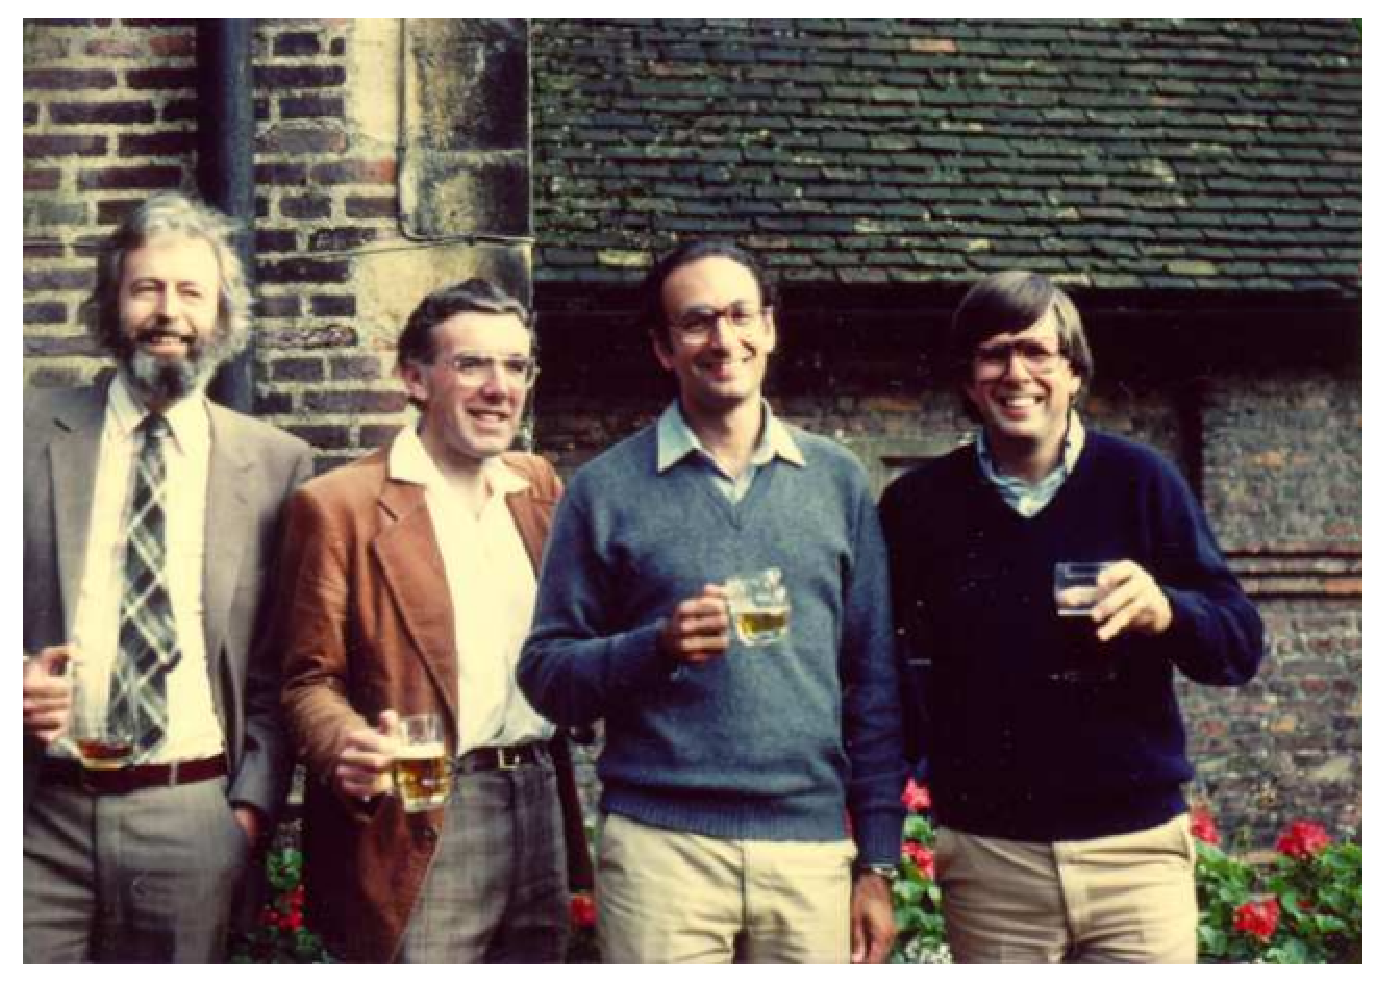
\includegraphics[width=0.55\textwidth,height=6cm]{figures/scientists/bfgs.eps}\\
  \caption{Army of Four: Broyden-Fletcher-Goldfard-Shanno}\label{fig:bfgs}
\end{figure}

\section{分枝定界法}
1960年,Ailsa Land与Alison Doig\cite{land1960automatic}创立\textbf{分枝定界法}(Branch and Bound Method),它是解决整数规划问题最常用的一种算法,也可求解混合整数线性规划问题(MILP)。以最小化目标函数的线性规划问题为例,假设$S$是问题的可行解集合,分枝定界法主要包括三个基本环节:\textbf{分枝}(Branching)、\textbf{定界}
(Bounding)与 \textbf{剪枝}(Pruning)。在分枝阶段,将$S$ 分割成多个相互不交的子集$S_1,S_2,\cdots$,满足$S=\mathop\bigcup\limits_i S_i$,并计算目标函数在每个子集上的最小值点;定界阶段计算目标函数在每个子集的上界与下界;分枝定界法法最关键的环节在于对可行解子集的筛选,即剪枝环节。在剪枝环节,根据目标函数在定界阶段的计算结果可以判定,如果目标函数值在子集甲上的下界比在子集乙的上界都要大,可以直接舍弃子集甲。分枝定界法通过多次调用分枝、定界与剪枝三个环节,逐渐逼近最优解。

在实际使用时,可以设计一定的启发式规则,当目标函数值上界与下界的差值比较接近时,则提前终止分枝步骤,从而大幅减少搜索时间。
\section{割平面法}
20世纪50年代,Ralph Gomory提出\textbf{割平面法}(Cutting-Plane Method)。

\section{随机搜索算法}
随机搜索算法(Random Search)对于目标函数的连续性、可微性无任何限制,是最简单、最直观的一种搜索算法。随机搜索一说最早源自
\cite{anderson1953recent,rastrigin1963convergence,karnopp1963random}。 随机算法迭代地从一个点移动到另一个点,以期后一个点相对于目标函数优于前者。随机搜索算法可概括为如下基本流程:
\begin{algorithm}[htbp]
        \caption{随机搜索算法}
        \begin{algorithmic}
            \REQUIRE ~~初始点$x$,最大迭代次数$T$,偏差阈值$\epsilon$\\
            \REPEAT
            \STATE
            \begin{itemize}
              \item 从超球面$\mathcal{S} = \{x|x\in \mathbb{R}^n, \|x - x_{t-1}\| = \delta_t\}$ 中抽取数据点$y$
              \item 如果$f(y) < f(x)$,则设置临时最优点$x=y$
            \end{itemize}
            \UNTIL{$t \le T$或者$f(x)-f(y)> \epsilon$}
            \ENSURE ~~ $x$是最优点
        \end{algorithmic}
\end{algorithm}

随机搜索算法在机器学习领域中应用广泛,经常使用的随机搜索方法有:模拟退火算法(Simulated Annealing)、遗传算法(Genetic Algorithms)、进化优化(
Evolutionary Programming)、粒子群优化算法(Particle Swarm Optimization)、蚁群优化(Ant Colony Optimization)、交叉熵(Cross Entropy)、随机近似算法(Stochastic Approximation)、多点搜索算法(Multi Start)、禁忌搜索算法(Tabu Search, Taboo Search)\cite{glover1990tabu}等。

随机搜索算法因其简单易于实现的特性,得到广泛应用。对于大型优化问题,相比确定性算法(如分支界定法)随机搜索算法则略胜一筹,遗憾之处在于它无法保证渐进收敛到最优解,只能通过大量的试错搜索,依概率收敛到某个未必全局最优的点。

\subsection{模拟退火算法}
在热力学中,“退火”(Annealing)是指物体缓慢降温的物理现象,温度越低,则物体的能量就越低。当温度下降到一定程度后,液体开始冷凝与结晶,在结晶状态,系统能量达到最低。如果物体快速降温,亦称“淬火”(Quenching),则可能产生能量不是最低的非结晶态。退火过程使得物体分子在任何温度下,都能有充足的时间、以较大的概率找到使其内能更低的位置,最终系统也最稳定。

1953年,Metropolis等人\cite{metropolis1953equation}提出使用蒙特卡洛模拟(Monte Carlo Simulation)方法确定热槽中分子的稳态分布。他们在模拟中使用的规则是:给定一个能量为$E_1$ 的状态$S_1$,如果此时移动一个分子的位置,系统状态发生转移,从$S_1$转移到$S_2$,能量从$E_1$变成$E_2$。如果$E_2 - E_1 \le 0$,则接受此状态。反之,如果能量升高(恶化状态),系统不会直接拒绝新状态$S_2$,而是以概率$\exp(\frac{E_2-E_1}{\kappa T})$有条件地接受它,其中$\kappa>0$是Boltzmann常数,$T$表示热槽的温度。通过不断重复这一流程,他们推断:在给定的温度$T$下,分子能量满足标准的Boltzmann分布:
\begin{equation}
    P(E = E(S)) = \frac{1}{Z(T)} \exp\big(-\frac{E(S)}{\kappa T}\big)
\end{equation}
其中,$E$是代表分子能量的随机变量,$Z(T)$是标准化因子:
\[
    Z(T) = \sum\limits_{S\in \mathcal{S}} \exp\big(-\frac{E(S)}{\kappa T}\big)
\]
这个公式就是著名的\textbf{Metropolis准则}。

根据推断,在温度$T$时,分子从状态$S_1$到$S_2$,能量从$E_1$变成$E_2$。根据Boltzmann分布可以计算两种状态下的概率差值:
\[
    \Delta P = P(E = E_2) - P(E = E_1) = \frac{1}{Z(T)} \exp\big(-\frac{E_2}{\kappa T}\big)\big[1-\exp\big(\frac{E_2 - E_1}{\kappa T}\big)\big]
\]
如果$E_1<E_2$,由于$\Delta E = E_2 - E_1 > 0$,则$\exp\big(\frac{E_2 - E_1}{\kappa T}\big) > 1$,从而$\Delta P < 0$。由此可以说明,温度不变时,分子停留在低能量状态$S_1$的概率比停留在高能量状态$S_2$的概率要大。根据Boltzmann分布可知,温度越高,不同能量状态对应的概率相差就越小,当温度足够高时,不同能量状态下的概率基本相同。随着温度下降,低能量状态对应的概率越来越大,当温度趋于0时,其概率达到1。

1983年,Scott Kirkpatrick等人\cite{kirkpatrick1983optimization}首次将模拟退火(Simulated Annealing)同组合优化(Combinatorial Optimization)联系起来。他们将能量对应到成本函数,将系统状态对应到组合优化问题的解,系统中粒子的一次移动等价地视为组合优化问题中的一次试验(Trial)。系统温度在组合最小化问题中就是一个控制参数,首先“冷却”处于高温条件下的解空间,然后,逐渐降温直至系统在一个稳定解“结晶”。
1985年,Vlado \u{C}ern\'{y}\cite{vcerny1985thermodynamical}独立地发现可将模拟退火原理应用于货郎担问题(Traveling Salesman Problem, TSP),并取得巨大成功。

模拟退火算法(Simulated Annealing Algorithm)能够实现全局最优或近似全局最优,奥秘就在于其接受状态的策略:除了接受优化解,还使用一个随机接受准则(\textbf{Metropolis准则})有限度地接受恶化解(Deterioration)。模拟退火算法能够逃脱局部最优点的园囿,很大程度上归功于那些看似不利状态的功劳,实现全局最优或接近全局最优。

\begin{algorithm}[htbp]
        \caption{模拟退火算法}
        \begin{algorithmic}
            \REQUIRE ~~系统温度$T$,允许最低温度$T_0$,迭代最大次数$N$,初始解$x_1$,Boltzmann常数设为$0<\kappa<1$\\
            \REPEAT
            \STATE
            \begin{enumerate}
                \item 从当前解$x_1$的邻域中随机选择点$x_2$,计算$\Delta E \triangleq f(x_2) - f(x_1)$
                \item 如果$\Delta E < 0$,则接受$x_2$为新解;否则,以概率
                \[
                    P = \exp(\frac{-\Delta E}{T})
                \]
                接受$x_2$。具体地,判定$P > \rand(0,1)$是否成立。若成立,则接受$x_2$;否则,拒绝$x_2$。
                \item 以速率$\kappa$降温:$T \leftarrow \kappa T$
                \item $i--$
            \end{enumerate}
            \UNTIL{$i<0$或$T<T_0$}
        \end{algorithmic}
\end{algorithm}
%如果$T=0$,模拟退火算法就退化为普通的贪婪搜索算法。

模拟退火算法至少有两个重要的控制参数:初始温度$T$和Boltzman常数$\kappa>0$,需谨慎选择与调整。它们主要从下面几点影响算法搜索的进程:
\begin{enumerate}[(1)]
  \item 初始温度$T$的设置问题:初始温度的设置是影响模拟退火算法全局搜索性能的重要因素之一,初始温度高,则搜索到全局最优解的可能性大,但需要消耗大量的计算时间;反之,效率增高但搜索性能可能受到影响。在实际应用中,初始温度一般需根据多次实验结果进行选择,比如
      David Fogel\cite{fogel1988evolutionary}在处理TSP问题时,根据100条随机产生的路线,取出最短与最长距离$d_0,d_1$,并使用下面公式设定初始温度:
      \[
        T = -(d_1-d_0)/\log 0.9
      \]
  \item 退火管理问题(Annealing Schedule):模拟退火算法全局搜索性能也和退火管理方式密切相关。一般而言,在同一温度下“充分”搜索(退火)是相当必要的,但需要计算开销。在实际应用中,需要针对具体问题的不同性质和特征设置合理的退火平衡条件。
\end{enumerate}

在模拟退火算法构造新解、接受新解过程,存在几个细节性的问题需要注意:(1)新解的产生一般是对当前解的一种简单变换,比如改变当前解的部分元素(逆序、交换、插入等),相比重新完全生成时间开销要小。(2)计算当前解与新解的目标函数之差时,如果能够分离出变换部分对目标函数差的独立影响,则目标函数差的计算就可以采用增量方式。(3)当确定接受新解时,需要以新解代替当前解。若已知产生新解的变换流程,可只就变换部分进行替换,从而节省完全替换的时间。

模拟退火算法确定的最优解与初始解无关,具有渐近收敛性,从理论上被证明是一种依概率$1$收敛于全局最优解的全局优化算法,此外模拟退火算法具有并行性。

\subsection{遗传算法}

\section{网格搜索算法}
网格搜索算法(Grid Search Algorithm)将搜索空间划分成网格状,根据各个格点处的目标函数值,选择出最优的解。在二维搜索空间(两个参数)中,网格搜索算法可以迅速确定最佳格点,但代价不菲,极易带来维数灾难问题:对于含有多个参数(比如$d$个)的优化问题,若沿着搜索空间每个坐标选取$1,000$的网格点,则产生的格点总数达到$m=1.0\times 10^{3d}$,相应地需要对目标函数评估$m$次。

如果待估的目标函数仅含少许几个参数,并且评估目标函数的代价低廉,那么网格搜索就是最佳的选择。反之,则可考虑使用网格游走(Grid Walk)或Nelder-Mead 算法。

\subsection{网格游走算法}
网格游走算法(Grid Walk)同网格搜索算法类似,但它不会搜索整个网格空间,而是从当前位置出发,根据其周围有限个邻居点上的目标函数值,选择“走下山”(Walk Down Hill)的下一站。

假设当前位置是$x=(x_1,x_2,\ldots, x_d)$,每次移动的步长为$s$,网格游走算法保持其他坐标值不变,在每个坐标当前位置往前或往后一步的地方评估目标函数:
\begin{equation}
    \left\{
    \begin{array}{lll}
      f_1^{-} & = & f(x_1 + s, x_2,\ldots, x_d) \\
      f_1^{-} & = & f(x_1 - s, x_2,\ldots, x_d) \\
      f_i^{+} & = & f(x_1, \ldots, x_{i-1}, x_i + s, x_{i+1}, \ldots, x_d), 2\le i \le d-1 \\
      f_i^{-} & = & f(x_1, \ldots, x_{i-1}, x_i - s, x_{i+1}, \ldots, x_d), 2\le i \le d-1 \\
      f_d^{+} & = & f(x_1, x_2,\ldots, x_d + s) \\
      f_d^{-} & = & f(x_1, x_2,\ldots, x_d - s) \\
    \end{array}
    \right.
\end{equation}
如果当前位置是最佳的,则减小步长(比如减半),再重复上述步骤。如果某个邻居格点是最佳的,则游走到此位置,继续依此策略进行搜索
\footnote{著名数学家George P\'{o}lya于1921年证明了一个有趣的定理:\textbf{喝醉的酒鬼总能找到回家的路,喝醉的小鸟则可能永远也回不了家}。
游走空间的维度越高,回到出发点的概率则越低。事实上,酒鬼在网格状分布的街道中随机游走,始终能够回到出发点,然而小鸟在三维网格中随机游走,就不那么幸运了,它最终回到出发点的概率只有大约34\%。在四维网格中随机游走,最终能回到出发点的概率是19.3\%,在八维空间概率仅为7.3\%。}
。网格游走算法每次仅需评估$2d$个邻居格点,维数灾难问题自然可以避免,优化的效率远高于网格搜索算法,在高维参数空间,更是如此。

网格游走算法通过不断缩小搜索范围,逐渐逼近局部最优点。在具体实现时,需要设置一个步长下限$s_0>0$,当步长缩减至$s<s_0$,则可以停止游走,结束搜索过程。为有效反映不同坐标(对应一个参数)的特征,对于每个坐标可以灵活地选择不同步长。

美中不足的是,网格游走算法易陷入局部最优点,为此,可以与随机搜索算法融合,通过引入随机因素弥补此一缺憾。

\section{坐标轮换法}
坐标轮换法(Univariate Search)是由D'Esopo\cite{desopo1959convex}在1959年发明的。坐标轮换法每次搜索只允许一个变量变化,其他变量保持不变,沿坐标方向轮流进行搜索的寻优方法。使用坐标轮换法搜索目标函数$f(x)$的最小值点,基本流程可概括如下:

\begin{algorithm}[htbp]
        \caption{坐标轮换法}
        \begin{algorithmic}
            \REQUIRE ~~初始点$x_1$,迭代次数$T$,允许误差$\epsilon>0$\\
            \FOR{$t = 1,\ldots, T$}
            \STATE
            \begin{enumerate}
                \item 取$y_1 = x_t$,从$y_1$出发,依次沿第$k(1\le k\le n)$个坐标轴方向做最优一维搜索:
                \[
                    f(y_k + \lambda_k e_k) = \min\limits_{\lambda>0} f(y_k + \lambda e_k)
                \]
                其中,$y_{k+1} = y_k + \lambda_k e_k$。
                \item 如果$\|y_{n+1} - y_1\| \ge \epsilon$,取$x_{t+1} = y_{n+1}$,结束本次迭代。
                \item 如果$\|y_{n+1} - y_1\| < \epsilon$,则迭代终止,$y_{n+1}$是$f(x)$的近似最小值点。
            \end{enumerate}
            \ENDFOR
        \end{algorithmic}
\end{algorithm}

\section{共轭方向法}
1964年,Michael Powell\cite{powell1964efficient}对坐标轮换法进行改进,提出了共轭方向法(Conjugate Direction Method),也称Powell方法。Powell方法主要包括基本搜索、加速搜索和搜索方向调整三部分,具体步骤如下:
\begin{algorithm}[htbp]
        \caption{Powell方法}
        \begin{algorithmic}
            \REQUIRE ~~初始点$x_0$,由$n$个相互线性无关的搜索方向构成的初始方向组$\{h_0,h_1,\ldots, h_{n-1}\}$,终止阈值$\epsilon>0$,取$k=0$\\
            \FOR{$k = 1,2,\ldots$}
            \STATE
            \begin{enumerate}
                \item \textbf{基本搜索}:令$y_0 = x_k$,依次沿着$h_0,h_1,\ldots, h_{n-1}$的方向进行一维搜索,得到相应的辅助迭代点$\{y_1,\ldots, y_n\}$:
                \[
                    y_i = y_{i-1} + \lambda_{i-1} h_{i-1}
                \]
                其中,$\lambda_{i-1} = \argmin\limits_{\lambda\ge 0} f(y_{i-1} + \lambda_{i-1} h_{i-1}),i=1,\ldots,n$
                \item \textbf{加速搜索}:令$h_n = y_n - y_0$,若$\|h_n\|\le \epsilon$,停止迭代,取下个迭代点$x_{k+1} = y_n$,否则转到下一步。
                \item \textbf{搜索方向调整}:取$\Delta_{m-1} \triangleq f(y_{m-1}) - f(y_m) = \max\limits_{i\in\{1,\ldots,n\}} f(y_{i-1}) - f(y_i)$,如果
                \[
                    f(2y_n - y_0) - [2f(y_n) - f(y_0)] \ge 2 \Delta_{m-1}
                \]
                成立,则搜索方向无需调整,令$x_{k+1} = y_n$;否则,转入下一步。
                \item \textbf{搜索方向组调整}:令$x_{k+1} = y_n + \lambda_n h_n$,其中
                \[
                    \lambda_n = \argmin\limits_{\lambda\ge 0} (y_n + \lambda h_n)
                \]
                丢弃第$m$个搜索方向向量:
                \[
                    \{h_0,\ldots, h_{m-1}, \textcolor{red}{h_m}, h_{m+1},\ldots, h_{n-1}\} \leftarrow \{h_0,\ldots, h_{m-1}, h_{m+1}, h_{m+2}, \ldots, h_{n}\}
                \]
            \end{enumerate}
            \ENDFOR
        \end{algorithmic}
\end{algorithm}

Powell方法是一种高效的零阶优化方法,但事无绝对,在某些条件下其表现不尽如人意。当一个搜索方向不能提供进一步的改善,则接下来的搜索方向就不再是共轭的。有时,在迭代几步以后,搜索方向可能平行。

\section{Nelder-Mead法}
1965年,John Nelder和Roger Mead\cite{nelder1965simplex}提出一种启发式局部搜索算法 -- Nelder-Mead法,有时也称“下山单纯形法”(Downhill Simplex Method)。一般地,Nelder-Mead法只需计算一个或两个点处的函数值,因此广泛应用于函数值计算开销较大的情形。

Nelder-Mead法使用单纯形(见\ref{sec:simplexmethod}节:Dantzig的单纯形法)的概念优化含有多个参数的目标函数。在搜索过程中,始终维护一个大小为$d+1$ 的顶点集,利用四种基本的变形规则(反射、扩展、收缩和压缩),灵活调整单纯形搜索方向。Nelder-Mead单纯形算法主要步骤如下:

\begin{enumerate}
  \item 初始化单纯形$\mathcal{S} = \mathcal{S}_0$:任意选取点$x_1\in \mathbb{R}^n$,根据给定步长$s_i$,选取$x_i = x_1 + s_i e_{i-1},i = 2,\ldots, n+1$,其中$e_i$ 表示第$i$维坐标的单位坐标基。
  \item \textbf{排序}(Order):对单纯形各顶点按函数值排序,不失一般性,假设
    \[
        f(x_1) \le f(x_2) \le \cdots \le f(x_n) \le f(x_{n+1})
    \]
  \item \textbf{中心点}(Centroid):计算除$f(x_{n+1})$以外的其他顶点的中心点
    \[
        c = \frac{1}{n} \sum\limits_{i=1}^{n} x_i
    \]
  \item \textbf{变形}(Transformation):根据各顶点函数值,改变当前单纯形形状。首先尝试利用“反射(Reflection)”、“扩展(Expansion)”、“收缩
  (Contraction)”搜索一个比$x_n$更好的顶点替换它,搜索的点皆位于由$x_{n+1}$和$c$确定的直线上。如果搜索成功,将使用新点替换$x_{n+1}$,结束本次迭代;否则,向顶点$x_1$方向“压缩(Shrink, Reduce)”单纯形$\mathcal{S}$。 具体做法如下:
      \begin{itemize}
        \item \textbf{反射}:选择反射点$x_r = c + \alpha (c - x_{n+1})$,其中$\alpha>0$。
            \textcolor{blue}{如果$f(x_1) \le f(x_r) < f(x_{n})$},则将使用$x_r$从$\mathcal{S}$中替换出$x_{n+1}$,并结束本次迭代。
        \item \textbf{扩展}:\textcolor{blue}{如果$f(r)<f(x_1)$},表明此方向利于搜索,于是选择扩展点$x_e = c + \gamma (c - x_{n+1})$,其中,
            $\gamma > \alpha$。如果$f(x_e) < f(x_r)$,则使用$x_e$替换$x_{n+1}$;否则,使用$x_r$替换$x_{n+1}$。结束本次迭代。
        \item \textbf{收缩}:\textcolor{blue}{如果$f(r) \ge f(x_n)$},表明此方向不利于搜索,转向$x_{n+1}$方向收缩。选择收缩点
            $x_c = c + \rho (c - x_{n+1})$,其中$\rho<0$。
            如果$f(x_c) < f(x_{n+1})$,则使用$x_c$替换$x_{n+1}$,并结束本次迭代;否则,“压缩”单纯形。
        \item \textbf{压缩}:如果利用“反射”、“扩展”、“收缩”搜索失败,表明最佳点$x_1$可能临近局部最优点,可以缩小搜索范围,选择向顶点$x_1$ 方向“压缩”单纯形,更新除$x_1$ 以外的所有顶点($\sigma > 0$):
          \[
            x_i \leftarrow \sigma (x_i + x_1), i = 2,\ldots, n+1
          \]
          更新单纯形$\mathcal{S}$后,结束本次迭代。
      \end{itemize}
\end{enumerate}

Nelder-Mead单纯形算法中使用的参数,一般分别取$\alpha=1,\gamma=2, \rho=-0.5, \sigma=0.5$。算法的终止条件,可选择在单纯形最短的边低于某个阈值。如果搜索空间有界,阻止单纯形法越界搜索最简单的法子,可以令越界点的函数值最不可能最优,比如最小化问题则越界点处函数值越大越好,最大化问题则函数值越小越好。

Nelder-Mead算法同网格搜索算法类似,都属于局部搜索方法,但它从多个角度对改进了网格搜索方法。比如,适应性地调整步长,使用更少的目标函数估计。单纯形算法与网格游走相似,对于初始点(单纯形)的选择十分敏感,选择的初始点不同,则可能得到不同的局部最优点。对于单纯形法,如果初始单纯形太小,很容易陷入局部最优。随机搜索算法、网格搜索算法比较擅长寻找起始点,但收敛速度不容乐观。加州伯克利大学教授Jonathan Shewchuk
\footnote{Jonathan Shewchuk:\href{http://www.cs.berkeley.edu/\~jrs/4/lec/23}{http://www.cs.berkeley.edu/$sim$jrs}}
提出融合两种类型的搜索算法,实现优势互补:(1)使用网格搜索(粗糙网格)寻找初始点,然后运行网格游走算法,并将网格搜索算法使用的步长减半。(2)使用网格搜索寻找多个(比如20个)表现好的起始点,然后将这些点分散到网格中,并选择其中一个点作为起始点,开始单纯形搜索,重复执行多次,优选出表现最好的点。

\section{Levenberg-Marquardt算法}
Levenberg-Marquardt优化算法,也称阻滞的最小二乘法,由Levenberg~\cite{levenberg1944method}和Marquardt~\cite{marquardt1963algorithm}两人分别在1944 年和1963年提出。它是使用最广泛的非线性最小二乘算法,主要处理非线性最优化问题。它介于牛顿法和梯度下降法之间,比牛顿法更健壮但收敛速度要慢,在非线性曲线拟合、计算机视觉等领域得到广泛应用。

给定一组数据$\{x_i,y_i\}_{i=1}^n$,$x_i\in \mathbb R^m$,$y_i\in \mathbb R$,曲线拟合的目的是
使用一个含参函数
\begin{equation}
    f_{\theta}:\mathbb R^m \mapsto \mathbb R
\end{equation}
拟合指定数据。$\theta\in \mathbb R^k$表示参数向量。函数对数据的拟合效果可以使用下面形式的误差平方和衡量:
\begin{equation}
    L(\theta) = \frac{1}{2}\sum\limits_{i=1}^n (f_{\theta}(x_i) - y_i )^2
\end{equation}
其中,系数$1/2$只是方便计算,不影响结果。模型参数的估计是通过最小化误差平方和实现的,此类方法因此被称作最小二乘法,当$f$是非线性函数时,称为非线性最小二乘法。

在实际应用中,人们有时会使用加权误差平方和(卡方)
\begin{equation}
    \chi^2(\theta) = \frac{1}{2}\sum\limits_{i=1}^n (\frac{f_{\theta}(x_i) - y_i}{\omega_i} )^2
\end{equation}
估计模型参数
\begin{equation}
    \theta = \argmin\limits_{\theta\in \Theta} \chi^2(\theta)
\end{equation}
其中,$\omega$表示误差权值向量,$\Theta$表示参数空间。

由于目标函数是可微的,我们计算它关于参数$\theta$的导数:
\begin{equation}
    \frac{\partial \chi^2(\theta)}{\partial \theta} = \sum\limits_{i=1}^n (\frac{f_{\theta}(x_i) - y_i}{\omega_i^2}) \frac{\partial f_{\theta}(x_i)}{\partial \theta} = (\hat{y}_{\theta} - y)^T W J
\end{equation}
其中,$\hat{y}_{\theta}\in \mathbb{R}^n$表示函数估计结果,$y\in \mathbb{R}^n$表示真实数据向量,$W$表示权值矩阵,对角线部分是$1/\omega_i^2$,$J$表示雅克比矩阵。

根据梯度下降法,可行的搜索方向为
\begin{equation}
    d_{gd} = J^T W (y-\hat{y}_{\theta})
\end{equation}
根据Gauss-Newton法,搜索方向$d_{gn}$有下面等式成立:
\begin{equation}
    J^T W J d_{gn} = J^T W(y-\hat{y}_{\theta})
\end{equation}
Levenberg-Marquardt算法则介于两者之间,选择的搜索方向$d_{lm}$满足:
\begin{equation}
    (J^T W J + \lambda I) d_{lm} = J^T W(y-\hat{y}_{\theta})
\end{equation}
其中的调节参数$\lambda$越大,则越接近于梯度下降法,$\lambda$越小,则越接近于Newton法。

Marquardt~\cite{marquardt1963algorithm}使用下面的形式更新模型参数:
\begin{equation}
    (J^T W J + \lambda \diag(J^T W J)) d_{lm} = J^T W(y-\hat{y}_{\theta})
\end{equation}

\section{信赖域方法}%Trust Region Method

\section{罚函数法}
利用罚函数法(Penalty Function Method),可将非线性规划问题的求解,转化为求解一系列无约束极值问题,因而也称\textbf{序列无约束最小化技术}(Sequential Unconstrained Minimization Technique, SUMT)。罚函数法求解非线性规划问题的思想:利用问题中的约束函数作出适当的罚函数,由此构造出带参数的增广目标函数,把问题转化为无约束非线性规划问题。罚函数法有两种形式,一种是外罚函数法,另一种是内罚函数法。

\section{障碍函数}
障碍函数(Barrier Function)是一个连续函数,当数据点趋近于可行域(Feasible Region)边界时,函数值增加到无穷。在有约束优化(Constrained Optimization)问题中,障碍函数可以用作违反约束条件的惩罚项,以防迭代过程搜索路径逃离出可行域。最常见的两种障碍函数是倒数障碍函数(Inverse Barrier Functions)和对数障碍函数(Logarithmic Barrier Functions)\footnote{由于对数障碍函数与主对偶内点法(Primal-dual Interior Point Method)存在联系,人们开始加深对数障碍函数的研究;倒数障碍函数相比而言,计算开销较大,因此,对数障碍函数更为实用}。

我们首先给出障碍函数的基本数学定义:
\begin{definition}\label{def:cone}
集合$K\subset \mathbb{R}^n$称为\textbf{锥},如果对于每一个$x\in K$,都有$tx\in K$,$\forall t\ge 0$。如果锥$K$是凸的,则称它为凸锥。
\end{definition}

\begin{definition}\label{def:barrier}
假设$K$是一个凸锥,如果连续函数$f:K \mapsto \mathbb R \bigcup \{+\infty\}$满足条件
\[
    \left\{
    \begin{array}{ll}
      f(x) < +\infty, & x\in int(K), \\
      f(x) = +\infty, & x\in bdry(K).
    \end{array}
    \right.
\]
我们称它是\textbf{障碍函数},其中$int(K)$表示$K$的内部(Interior),$bdry(K)$表示$K$的边界(Boundary)。如果障碍函数形如$f(x) = -\log\phi(x)$,并且$\phi: K \mapsto \mathbb R^{+}$也是一个连续函数,则我们称它\textbf{对数障碍函数}\cite{frisch1955logarithmic}。
\end{definition}

对于下面的原始优化问题:
\begin{equation}
    \begin{array}{ll}
      \min & c^T x \\
      \textit{s.t.} & Ax \le b
    \end{array}
\end{equation}
其中,$A=(a_1,\ldots, a_m)^T$,则可以定义如下形式的障碍函数:
\begin{equation}\label{eq:barrierfunction}
    f(x) = \left\{
    \begin{array}{rl}
      -\sum\limits_{i=1}^m \log(b_i - a_i^T x), & Ax < b, \\
      +\infty, & Ax \ge b.
    \end{array}
    \right.
\end{equation}

将有约束优化问题转化成下面的无约束优化问题:
\[
    \min~~c^T x + \lambda f(x)
\]

\section{范数逼近}
范数逼近(Norm Approximation)在信号处理、压缩感知(Compressed Sensing)\footnote{压缩感知也称压缩采样或稀疏采样,属于一种新的采样理论,2004年由斯坦福大学教授Emmanuel Candes、美国科学院院士David Donoho、菲尔兹奖获得者陶泽轩等学者提出。它能够利用信号的稀疏性特征,随机采样获取信号的离散样本,通过非线性重建算法重建原始信号,在信息论、图像处理、光学成像、模式识别等领域受到高度关注,并被美国科技评论评委2007年度十大科技进展。}等领域中有很多应用
\cite{cipra2006l1},\cite{grant2006disciplinedconvex}对解决范数最优化问题有过概述,主题是将无约束的范数最小化问题转化为线性规划问题,本节我们做出简要介绍。

Cipra认为\cite{cipra2006l1},$\ell_1$与$\ell_0,\ell_2$之间存在着重要的关联。$\ell_1 = \sum\limits_i |x_i|$是联系二者的纽带,它同时具有$\ell_0=\sum\limits_i I(x_i \ne 0)$稀疏敏感、$\ell_2 = \sum\limits_i x_i^2$方便计算的良好性质。$\ell_0$在构建稀疏性模型(复杂度小)时,有着重要的应用;$\ell_2$在模型优化问题中使用广泛。

%-------------mathematics (optimisation, matrix, graph)
\chapter{统计学}
统计学萌芽于欧洲,16世纪伽利略Galileo Galilei为解答赌徒们的问题,提出了概率论的基本原理。17世纪中叶,帕斯卡Blaise Pascal
\footnote{布莱斯·帕斯卡Blaise Pascal(1623 $\sim$ 1662)是法国物理学家、哲学家和神学家,还是一位伟大的数学家和统计学家,他唯一留给世人的是载录其理论思想的《思想录》,虽未形成系统的理论框架,仍然具有重要的参考价值。他曾经提出了一个著名的赌注,深刻影响了概率论、决策论的诞生,并促进存在主义、实用主义、唯意志论发展,后人称之为“帕斯卡的赌注”(Pascal's Wager):上帝要么存在,要么不存在。如果你相信上帝的存在,那么最坏的可能就是上帝本不存在,则在死后进入虚无世界,你没有任何损失;若上帝确实存在,那么你将获得永生。如果你拒绝信仰,则最好的结果就是虚无,但最坏的结果就是承受永世的地狱之苦。一个理性的人,就应该相信上帝的存在。}
和费马Pierre de Fermat关于“得点问题”的讨论,奠定了\textbf{概率论}(Probability Theory)的基础。17世纪末18世纪初统计学开始蓬勃发展。19世纪末,由于英国探险家、人类学家和优生学家法兰西斯·高尔顿Francis Galton和统计学家卡尔·皮尔逊Karl Pearson的突出贡献,\textbf{描述统计学}(Descriptive Statistics)正式诞生。\textbf{推论统计学}
(Inferential Statistics)是研究如何根据样本数据去推断总体统计特征,先驱人物是英国统计学家威廉·格赛特William Sealy Gosset和罗纳德·费舍尔Ronald Aylmer Fisher。最初将统计学应用于教育与心理方面研究的是高尔顿,而对教育统计做出重要贡献的是心理学家查尔斯·爱德华·斯皮尔曼Charles Edward Spearman。

\ornamento

\section{概率论基础}
概率论与数理统计(Probability and Mathematical Statistics)研究的对象是随机现象。
在一定的条件下,并不总是出现相同结果的现象称为\textbf{随机现象}。随机现象的结果不止一个,并且人们事先并不知道哪个结果出现。如果只有一个结果,那么该现象称为\textbf{确定性现象}。在相同条件下可以重复的随机现象又称作
\textbf{随机试验}(Random Trial),比如抛硬币、掷骰子的试验等。自然界中还有很多无法重复的随机现象,比如某场球赛的输赢、某个时段的经济增长速度等。

随机现象的一切可能的基本结果组成的集合称作\textbf{样本空间}(Sample Space),记作$\Omega=\{\omega\}$,其中$\omega$表示基本结果,又称为样本点,也是抽样时的基本单元。样本空间至少有两个样本点,只含有两个样本点的样本空间是最简单的样本空间。如果样本点的数目有限或可数,则称该样本空间为离散样本空间;如果样本点的数目不可数,则称该样本空间是连续样本空间。

随机现象的某些样本点组成的集合称作\textbf{随机事件},简称\textbf{事件}。样本空间$\Omega$的最大子集(即$\Omega$自身)称作\textbf{必然事件}、最小子集(即空集$\emptyset$)称作\textbf{不可能事件}。用来表示随机现象结果的变量称作\textbf{随机变量}。

\begin{example}
骰子(亦作色子)是一种古老的赌具,多为正立方体六面骰,各面刻有一至六个点数,并且彼此相对的两面数字之和为七。骰子最早出现在两千年前的埃及,古埃及人称其“astragal”。在中国,相传骰子是由三国时的文学家曹植所发明,最初用作占卜工具,后来演变成后宫嫔妃的游戏,根据掷骰子的点数赌酒或赌丝绸香袋等物。当时骰子的点穴上涂的是黑色,唐代时增加描红。

赌场内的荷官摇掷骰子透过骰子的点数定输赢,每一场赌局投掷骰子的点数都可能不同。荷官投掷骰子的事件可以看作是一个随机事件,记作$X$,所有可能的投掷结果构成样本空间$\Omega=\{1,2,3,4,5,6\}$,“投掷的骰子点数大于4”的事件可以使用“$X>4$”表示。
\end{example}

随机事件的不同结果的发生存在不同程度的可能性,有些结果可能性大有些可能性小。概率论最基本的一个问题是定义随机事件的概率,以刻画事件发生的可能性。16世纪,意大利学者Gerolamo Cardano
\footnote{Gerolamo Cardano(1501--1576),意大利数学家、医学家、物理学家,统计学创始人。1526年获帕维亚大学医学博士学位,后成为欧洲名医,曾任英国国王爱德华六世的御医,并曾任教于帕维亚大学、博洛尼亚大学。他学识渊博,一生写作出版各类文章、书籍200多种,被誉为百科全书式的学者。
他的家庭生活非常不幸。他最喜爱的大儿子詹巴蒂斯塔因杀死不忠的妻子于1560年被判死刑。他的女儿沦为妓女,死于梅毒。他的另一个儿子是个赌徒,经常偷窃他的财物。他自己因为推算耶稣的出生星位,被指控为大逆不道,于1570年入狱,并失去教职。更为可悲的是,他的儿子参与了指控。出狱后他移居罗马,获得了教皇格里高利十三世(Pope Gregory XIII)的年金资助,完成了自己的自传。据说,他七十一岁时通过占星术推算出自己将在1576 年9月21 日去世,但是到那一天时,他活得像头壮牛;为了保全自己大星象学家的名声,他自杀了。}
开始研究赌博游戏中的一些简单问题,其死后发表的《论赌博游戏》(\textit{Liber de ludo aleae})给出了一些概率论的基本概念和定理,被认为是第一部概率论著作。在Cardano以后约三百年的时间里,Blaise Pascal、Pierre de Fermat、Jacob Bernoulli等数学家都在古典概率计算、公式推导和扩大应用等方面做了重要的工作。1812年,法国数学家Pierre-Simon Laplace在《概率的分析理论》(\textit{Th\'{e}orie analytique des probabilit\'{e}s})中给出概率的古典定义:事件$A$的概率等于一次试验中出现事件$A$的可能结果数目与该事件中所有可能结果数目之比。古典定义通过简单明了的方式定义了事件的概率,并给出简单可行的方法。古典定义是在经验事实的基础上,对被考察事件的可能性进行逻辑分析后得到的事件概率。古典定义的基本假设有两个:(甲)随机事件可能结果总数有限;(乙)每个结果的出现有同等可能。Jacob Bernoulli在研究古典概率时发现Bernoulli大数定律,即“频率具有稳定性”,从而可以“用频率估计概率”。

概率论发展的历史,诞生过概率的古典定义、概率的几何定义、概率的频率定义和概率的主观定义。1900年,38岁的德国数学家David Hilbert在世界数学家大会上提出建立概率公理系统的问题,也就是著名的Hilbert 23个问题中的第6个问题。20世纪初完成的勒贝格测度与积分理论,以及随后发展的抽象测度和积分理论,为概率论公理体系的建立奠定了基础。1933年,前苏联数学家Andrey Kolmogorov\cite{Kolmogorov1951Foundations}运用集合论和测度论正式给出概率严密的公理化定义,既概括了古典定义、统计定义的基本特性,又避免了各自的局限。概率论公理体系的出现是概率论发展史上的一个里程碑,至此概率论才真正成为严格的一个数学分支。

\begin{definition}[$\sigma$-代数与可测空间]
假设$\Omega$是一个样本空间,$\mathscr F$是$\Omega$的某些子集所构成的集合类(Collection)。如果$\mathscr F$满足:
\begin{itemize}
  \item $\Omega\in \mathscr F$;
  \item \textbf{余集封闭}:如果$A\in \mathscr F$,则$\bar A=\Omega\setminus A\in \mathscr F$;
  \item \textbf{可列并封闭}:如果$A_n\in \mathscr F$,$n=1,2,\ldots$,则$\bigcup\limits_{n=1}^{\infty}A_n\in \mathscr F$。
\end{itemize}
则称$\mathscr F$为\textbf{$\sigma$-代数}(Sigma-Algebra)、\textbf{Borel域}(Borel Field)或\textbf{事件域}(Field of Events),$(\Omega,\mathscr F)$称作\textbf{可测空间}(Measurable Space)。
\end{definition}
根据定义可以推知:
\begin{itemize}
  \item $\emptyset\in \mathscr F$;
  \item \textbf{差集封闭}:如果$A,B\in \mathscr F$,则$A\setminus B\in \mathscr F$;
  \item \textbf{有限交、有限并、可列交封闭}:如果$A_n\in \mathscr F$,$n=1,2,\ldots$,则$\bigcap\limits_{i=1}^n A_n, \bigcup\limits_{i=1}^n A_n, \bigcap\limits_{n=1}^{\infty}A_n\in \mathscr F$。
\end{itemize}

\begin{definition}[概率与概率空间]
假设$(\Omega,\mathscr F)$是可测空间,$P(\cdot)$是定义在$\mathscr F$上的实值函数,如果满足:
\begin{itemize}
  \item \textbf{非负性公理}:对任意的$A\in \mathscr F$,都有$0\le P(A)\le 1$;
  \item \textbf{正则性公理}:$P(\Omega)=1$;
  \item \textbf{可列可加性公理}:对于两两互不相容事件$A_1,A_2,\ldots$($A_i\cap A_j = \emptyset$,$i\ne j$)有:
  \[
    P(\bigcup\limits_{i=1}^\infty A_i) = \sum\limits_{i=1}^\infty P(A_i),
  \]
\end{itemize}
则称$P(\cdot)$是可测空间$(\Omega,\mathscr F)$上的\textbf{概率}(Probability),$P(A)$为事件$A$的概率,$(\Omega,\mathscr F, P)$称作\textbf{概率空间}
(Probability Space)。
\end{definition}
根据定义可以推知:
\begin{itemize}
  \item \textbf{可减性}:如果$A,B\in \mathscr F$且$A\subset B$,则$P(B\setminus A) = P(B) - P(A)$;
\end{itemize}
如果事件列$\{A_n, n\ge 1\}$满足$A_n\subset A_{n+1}$,则称作单调增列,有$\lim\limits_{n\rightarrow \infty} A_n = \bigcup\limits_{i=1}^{\infty} A_i$;
如果事件列$\{A_n, n\ge 1\}$满足$A_n\supset A_{n+1}$,则称作单减增列,有$\lim\limits_{n\rightarrow \infty} A_n = \bigcap\limits_{i=1}^{\infty} A_i$。
\begin{itemize}
  \item \textbf{概率连续性}:如果事件列$\{A_n, n\ge 1\}$是单调减列或单调增列,则
  \[
    \lim_{n\rightarrow \infty} P(A_n) = P(\lim_{n\rightarrow \infty} A_n).
  \]
\end{itemize}

概率的解释与定义在争议中不断向前发展,从
概率的公理化定义刻画了概率的本质,但是没有明确指出具体地确定概率的方法。在公理化定义之前的概率的频率定义、古典定义、几何定义和主观定义都在一定场合下,存在各自确定概率的方法。在公理化定义范畴下,一一对应确定概率的频率方法、古典方法、几何方法和主观方法。

\begin{definition}[条件概率]
假设$(\Omega,\mathscr F, P)$是概率空间,$B\in \mathscr F$,且$P(B)>0$,如果对任意的$A\in \mathscr F$,记
\[
    P(A|B) = \frac{P(AB)}{P(B)},
\]
则称$P(A|B)$为事件$B$发生的条件下,事件$A$发生的\textbf{条件概率}(Conditional Probability)。
\end{definition}
由条件概率的定义可知:
\begin{itemize}
  \item \textbf{乘法公式}:设$A,B\in \mathscr F$,则有$P(AB)=P(A|B)P(B)$。一般地,如果$A_i\in \mathscr F, i=1,2,\ldots,n$,且$P(A_1 A_2\cdots A_n)>0$,则有\[P(A_1 A_2\cdots A_n)=P(A_1)P(A_2|A_1)P(A_3|A_1A_2)\cdots P(A_n|A_1A_2\cdots A_{n-1}).\]
  \item \textbf{全概率公式}:设$(\Omega,\mathscr F, P)$是概率空间,$A\in \mathscr F$,$B_i\in \mathscr F$,$i = 1,2,\ldots,n$,$B_i\cap B_j=\emptyset (i\ne j)$,且$\bigcup\limits_{i=1}^n B_i = \Omega$,$P(B_i)>0$,则有
      \[
        P(A) = \sum\limits_{i=1}^n P(A|B_i) P(B_i).
      \]
  \item \textbf{贝叶斯定理\footnote{Thomas Bayes(1701--1761),英国数学家,生前是一位受人尊敬的英格兰长老会牧师。他是一位自学成才的数学家,1742 年入选英国皇家学会会员,1763年在一篇论文中首次提到贝叶斯定理。为了证明上帝的存在,他发展了一套成熟的概率方法论。他的思想和方法对概率统计的发展产生了深远的影响,至今在许多领域都还有广泛应用。}}:设$(\Omega,\mathscr F, P)$ 是概率空间,$A\in \mathscr F$,$B_i\in \mathscr F$,$i = 1,2,\ldots,n$,$B_i\cap B_j=\emptyset (i\ne j)$,且$\bigcup\limits_{i=1}^n B_i = \Omega$,$P(B_i)>0$,$P(A)>0$,则有
      \[
        P(B_i|A) = \frac{P(B_i)P(A|B_i)}{\sum\limits_{i=1}^n P(A|B_i) P(B_i)}.
      \]
      一般地,若对任意的$A_1,\ldots,A_n\in \mathscr F$,都有$P(\bigcap\limits_{i=1}^n A_i) =\prod\limits_{i=1}^n P(A_i)$,则称$\mathscr F$是独立事件簇。
\end{itemize}

\begin{definition}[随机变量及其分布函数]
假设$(\Omega,\mathscr F, P)$是概率空间,$X=X(\omega)$是定义在$\Omega$上的实值函数。如果对任意的$x\in \mathbb R$,都有$X^{-1}((-\infty,x])=\{\omega: X(\omega)\le x\}\in \mathscr F$,则称$X(\omega)$是$\mathscr F$上的\textbf{随机变量}(Random Variable),简记作$X$。$F(x) = P(X\le x)=P(\{\omega: X(\omega)\le x\})=P(X^{-1}((-\infty,x]))$称作随机变量$X$的\textbf{累积分布函数}(Cumulative Distribution Function, CDF),简称\textbf{分布函数}。
\end{definition}
根据随机变量的分布函数的定义,我们可以得到下面几条性质:
\begin{itemize}
  \item $F(x)$是增函数:当$x_1<x_2$时有$F(x_1)\le F(x_2)$;
  \item $F(-\infty) = \lim\limits_{x\rightarrow -\infty} F(x)=0$,$F(+\infty) = \lim\limits_{x\rightarrow +\infty} F(x)=1$;
  \item $F(x)$右连续。
\end{itemize}
随机变量有两种类型:离散型和连续型随机变量。离散型随机变量的概率分布可以使用\textbf{概率分布列}或曰\textbf{概率质量函数}(Probability Mass Function, PMF)表示:$p_k = P(X=x_k),k=1,2,\ldots$,其分布函数为$F(x)=\sum\limits_{x\le x_k} p_k$;连续型随机变量的概率分布用\textbf{概率密度函数}(Probability Density Function, PDF)$f(x)$来描述,其分布函数$F(x)=\int_{-\infty}^x f(t)dt$。

\begin{definition}[多维随机变量及其分布函数]
假设$(\Omega,\mathscr F, P)$是概率空间,$X_i=X_i(\omega), i=1,2,\ldots,n$都是定义在$\Omega$上的实值函数。如果对任意的$x_i\in \mathbb R$,都有$X_i^{-1}((-\infty,x_i])=\{\omega: X_i(\omega)\le x_i\}\in \mathscr F$,则称$X(\omega)=(X_1(\omega),X_2(\omega),\ldots,X_n(\omega))$是\textbf{$n$维随机变量}或\textbf{随机向量},简记作$X=(X_1,X_2,\ldots,X_n)$。$F(x_1,x_2,\ldots,x_n) = P(X_1\le x_1,X_2\le x_2,\ldots, X_n\le x_n)$称作随机变量$X$的
\textbf{联合分布函数}(Joint Cumulative Distribution Function,JCDF)。
\end{definition}

对于二维随机变量$(X,Y)$,其联合分布函数$F(x,y)=P(X\le x, Y\le y)$是事件$\{X\le x\}$与事件$\{Y\le y\}$同时发生的概率。
\begin{definition}[二维离散随机变量与联合分布列]
如果二维随机变量$(X,Y)$只取有限个或可数的$(x_i,y_i)$,则称$(X,Y)$为二维离散随机变量,称
\[
    p_{ij} = P(X=x_i, Y=y_i),~~~i,j=1,2,\ldots
\]
为$(X,Y)$的\textbf{联合分布列}(Joint Probability Mass Function, JPMF)。
\end{definition}
\begin{definition}[二维连续随机变量与联合密度函数]
如果存在二元非负函数$p(x,y)$,使得二维随机变量$(X,Y)$的分布函数$F(x,y)$可表示为
\[
    F(x,y)=\int_{-\infty}^x \int_{-\infty}^y f(u,v) dv du,
\]
则称$(X,Y)$为二维随机变量,称$f(u,v)$为$(X,Y)$的\textbf{联合密度函数}(Joint Probability Density Function, JPDF)。
\end{definition}

\begin{definition}[边际概率分布函数]
如果在二维随机变量$(X,Y)$的联合分布函数$F(x,y)$中取$y\rightarrow +\infty$,由于$\{Y<+\infty\}$是必然事件,则称
\[
    \lim\limits_{y\rightarrow +\infty} F(x,y) = P(X\le x, Y\le +\infty) = P(X\le x),
\]
是$X$的\textbf{边际概率分布函数}(Marginal Distribution Function),记为
\[
    F_X(x) = F(x,+\infty).
\]
类似地,$F_Y(y)=F(+\infty,y)$称作$Y$的边际概率分布函数。
\end{definition}

在二维离散随机变量$(X,Y)$的联合分布列$\{P(X=x_i,Y=y_j)\}$中,对$j$求和所得的分布列
\[
    \sum\limits_{j=1}^\infty P(X=x_i,Y=y_j)=P(X=x_i),~~~i=1,2,\ldots
\]
称作$X$的边际概率分布列。类似地,对$i$求和所得的分布列
\[
    \sum\limits_{i=1}^\infty P(X=x_i,Y=y_j)=P(Y=y_j),~~~j=1,2,\ldots
\]
称作$Y$的边际概率分布列。

如果二维连续随机变量$(X,Y)$的联合概率密度函数为$f(x,y)$,由于
\begin{eqnarray}
  \nonumber F_X(x) = F(x,+\infty) =\int_{-\infty}^x \Bigg(\int_{-\infty}^{+\infty} f(u,v)dv\Bigg) du \triangleq \int_{-\infty}^x f_X(u)du,\\
  \nonumber F_Y(y) = F(+\infty,y) =\int_{-\infty}^y \Bigg(\int_{-\infty}^{+\infty} f(u,v)du\Bigg) dv\triangleq \int_{-\infty}^y f_Y(v)dv,
\end{eqnarray}
其中$f_X(x)$和$f_Y(y)$分别称作$X$的边际概率密度函数、$Y$的边际概率密度函数(Marginal Density Function)。

\section{随机变量的数字特征}%Numerical Characteristics
\begin{definition}[数学期望]
假设$X$是定义在概率空间$(\Omega,\mathscr F, P)$上的随机变量,如果$\int_{\Omega} |X| dP <\infty$,就称$X$的\textbf{数学期望}(Expectation)或均值存在,或称$X$是可积的,记作$E(X)$,并有下列定义:
\[
    E(X) = \int_{\Omega} X dP.
\]
如果$X$是离散型随机变量,如果级数$\sum\limits_{i=1}^{+\infty} |x_i| p_i$收敛,则$E(X)=\sum\limits_{i=1}^{+\infty} x_i p_i$是随机变量$X$的数学期望。如果$X$是连续型随机变量,如果积分$\int_{-\infty}^{+\infty} |x| f(x)dx$收敛,则$E(X)=\int_{-\infty}^{+\infty} x f(x)dx$是随机变量$X$的数学期望。
\end{definition}

\begin{definition}[条件分布]
对一切使$f_Y(y)>0$的$y$,给定$Y=y$条件下$X$的条件分布函数(Conditional Distribution Function)和条件密度函数(Conditional Density Function)分别为
\begin{eqnarray}
  F(x|y) &=& \int_{-\infty}^x \frac{f(u,y)}{f_Y(y)} du,\\
  f(x|y) &=& \frac{f(x,y)}{f_Y(y)} = \frac{f_X(x) f(y|x)}{\int_{-\infty}^{+\infty} f_X(x) f(y|x) dx}.
\end{eqnarray}
\end{definition}

\begin{definition}[条件数学期望]
设$X$和$Y$是随机变量,对一切使$f_Y(y)>0$的$y$,给定$Y=y$条件下$X$的期望定义如下:
\[
    E(X|Y=y) = \int_{-\infty}^{+\infty} xf(x|y)dx.
\]
%http://www.cnblogs.com/murongxixi/p/3477962.html
%http://www.jdl.ac.cn/user/lyqing/StatLearning/Statistical09Fall.html
\end{definition}
条件期望$E(X|Y=y)$是$y$的函数,对$y$的不同取值,条件期望$E(X|Y=y)$的取值也在变化。为此,我们记$g(y) = E(X|Y=y)$。我们还可以将条件期望看做是随机变量$Y$的函数,记作$E(X|Y)=g(Y)$。

\begin{theorem}[重期望公式]
设$(X,Y)$是二维随机变量,且$E(X)$存在,则$E(X)=E(E(X|Y))$。
\end{theorem}
\begin{proof}
假设$(X,Y)$的联合密度函数是$f(x,y)$,由$f(x,y)=f(x|y)f_Y(y)$可得:
\[
\begin{array}{lcl}
    E(X) & = & \int_{-\infty}^{+\infty} \int_{-\infty}^{+\infty} x f(x,y) dx dy\\
    &=& \int_{-\infty}^{+\infty}\big(\int_{-\infty}^{+\infty} xf(x|y) dx\big) f_Y(y) dy\\
    &=& \int_{-\infty}^{+\infty} E(X|Y=y) f_Y(y) dy\\
    &=& \int_{-\infty}^{+\infty} g(y) f_Y(y) dy\\
    &=& E(g(Y)) = E(E(X|Y)).
\end{array}
\]
证毕。
\end{proof}
我们下面来看条件期望的一些基本性质:
\begin{property}[独立性]
如果$X$和$Y$是两个独立随机变量,则对于任意使$f_Y(y)>0$的$y$都有\[E(X|Y=y)=E(X).\]
\end{property}
\begin{proof}
由$X$和$Y$的独立性可知$f(x,y)=f_X(x) f_Y(y)$,则$f(x|y)=\frac{f(x,y)}{f_Y(y)} = f_X(x)$,按照条件期望的定义则有
\[
    E(X|Y=y) = \int_{-\infty}^{+\infty} xf(x|y) dx = \int_{-\infty}^{+\infty} x f_X(x) = E(X).
\]
证毕。
\end{proof}
\begin{property}
设$h$是一个实值函数,对于任意使$f_Y(y)>0$的$y$都有$E(h(Y)|Y)=h(Y)$。
\end{property}
\begin{proof}
对于任意的$y\in \mathbb R$,如果给定$y$,则条件概率$f(h(Y) = h(y) | Y=y)=1$。根据定义可知
\[
\begin{array}{lcl}
    E(h(Y)|Y=y) = h(y) f(h(Y) = h(y) | Y=y) = h(y),
\end{array}
\]
那么$E(h(Y)|Y)=h(Y)$。
\end{proof}

\begin{property}[线性相加性]
设$X_1$、$X_2$和$Y$都是随机变量,$\alpha_1,\alpha_2\in \mathbb R$,则
\[
    E(\alpha_1 X_1 + \alpha_2 X_2|Y=y)=\alpha_1 E(X_1|Y=y) + \alpha_2 E(X_2|Y=y).
\]
\end{property}
\begin{proof}
我们直接按照条件期望的定义推导:
\[
    \begin{array}{lcl}
        E(\alpha_1 X_1 + \alpha_2 X_2|Y=y) &=& \int_{-\infty}^{+\infty} \int_{-\infty}^{+\infty} \alpha_1 u + \alpha_2 v f(X_1=u, X_2=v|Y=y) dudv\\
        &=&\alpha_1 \int_{-\infty}^{+\infty} \int_{-\infty}^{+\infty} u f(X_1=u, X_2=v|Y=y) dudv + \\
        &&\alpha_2 \int_{-\infty}^{+\infty} \int_{-\infty}^{+\infty} v f(X_1=u, X_2=v|Y=y) dudv\\
        &=& \alpha_1 \int_{-\infty}^{+\infty}  u f(X_1=u|Y=y) du + \alpha_2 \int_{-\infty}^{+\infty}  v f(X_2=v|Y=y) dv\\
        &=& \alpha_1 E(X_1|Y=y) + \alpha_2 E(X_2|Y=y).
    \end{array}
\]
证毕。
\end{proof}

\begin{property}
设$X$和$Y$是随机变量,$g$和$h$是实值函数,则$E[g(X)h(Y)] = E[h(Y)E(g(X)|Y)]$。
\end{property}
\begin{proof}
根据条件期望的定义可以推导:
\[
    \begin{array}{lcl}
        E[g(X)h(Y)] &=& \int_{-\infty}^{+\infty} \int_{-\infty}^{+\infty} g(x) h(y) f(x,y) dxdy\\
        &=& \int_{-\infty}^{+\infty} h(y) f_Y(y) (\int_{-\infty}^{+\infty} g(x) f(x|Y=y) dx) dy\\
        &=& \int_{-\infty}^{+\infty} h(y) E(g(X)|Y=y) f_Y(y) dy\\
        &=& E[h(Y)E(g(X)|Y)].
    \end{array}
\]
证毕。
\end{proof}

\begin{definition}[原点矩和中心矩]
假设$g(x)$是$\mathbb R$上的Borel可测函数,若其数学期望存在$E(|g(x)|) < \infty$,则有
\[
    E(g(X)) = \int_\Omega g(X) dP = \int_{-\infty}^{+\infty} g(x) f(x) dx.
\]
如果$g(X)=X^k, k\in \mathbb N$的数学期望存在,就称
\[
    E(X^k) = \int_{-\infty}^{+\infty} x^k f(x) dx
\]
为$X$的\textbf{$K$阶原点矩}(K-th Moment about the Origin)。如果$g(X)=|X|^k, k\in \mathbb N$的数学期望存在,称
\[
    E(|X|^k) = \int_{-\infty}^{+\infty} |x|^k f(x) dx
\]
为$X$的\textbf{$K$阶绝对原点矩}(K-th Absolute Moment about the Origin)。如果$g(X)=(X-E(X))^k, k\in \mathbb N$的数学期望存在,称
\[
    E((X-E(X))^k) = \int_{-\infty}^{+\infty} (x-E(X))^k f(x) dx
\]
为$X$的\textbf{$K$阶中心矩}(K-th Central Moment)。如果$g(X)=|X-E(X)|^k, k\in \mathbb N$的数学期望存在,称
\[
    E(|X-E(X)|^k) = \int_{-\infty}^{+\infty} |x-E(X)|^k f(x) dx
\]
为$X$的\textbf{$K$阶绝对中心矩}(K-th Absolute Central Moment)。
\end{definition}

\begin{definition}[方差]
我们称随机变量$X$的\textbf{二阶中心矩}为\textbf{方差}(Variance),记作$\var(X)$,则有
\[
    \var(X) = E((X-E(X))^2) = \int_{-\infty}^{+\infty} (x-E(X))^2 f(x) dx =  E(X^2) - (E(X))^2.
\]
\end{definition}

\begin{theorem}
对于随机变量$X$,如果对任意的$k\in \mathbb N$都有$E(|X|^k)<\infty$,则对所有的正整数$i<k$都有$E(|X|^i)<\infty$。
\end{theorem}
\begin{proof}
假设随机变量$X$是连续的,并且其概率密度函数是$f(x)$,则对于$i<k$有
\[
\begin{array}{lcl}
    E(|X|^i) &=& \int_{-\infty}^{+\infty} |x|^i f(x) dx\\
    &=& \int_{|x|\le 1} |x|^i f(x) dx + \int_{|x|> 1} |x|^i f(x) dx\\
    &\le& \int_{|x|\le 1} f(x) dx + \int_{|x|> 1} |x|^k f(x) dx\\
    &\le& P(|X|\le 1) + E(|X|^k),
\end{array}
\]
根据假设$E(|X|^k)<\infty$,必然有$E(|X|^i) < \infty$。
\end{proof}
由此可知,只要$E(X^2)<\infty$,则变量$X$的期望和方差都存在。

如果我们知道随机变量的分布函数,就可以很容易地计算出随机变量的各种数值特征,如均值、方差和其他各高阶矩。通常,计算随机变量的各阶矩,往往要进行求和或积分运算。实际上,我们可以简化随机变量各阶矩的积分或加和运算,并建立起各阶矩的统一形式。我们下面介绍两个重要的分析工具:\textbf{矩母函数}(Moment Generating Function)与\textbf{特征函数}(Characteristic Function),它们可以把独立随机变量和分布的卷积运算转换为乘法运算,将随机变量各阶原点矩的计算转换成简单的微分计算,甚至可以将随机变量序列的极限分布转换成一般函数极限问题。

\begin{definition}[矩母函数]
设$X$是一个随机变量,函数
\[
    \psi(t) = E(e^{tX}) = \int_{-\infty}^{+\infty} e^{tx} f(x)dx, -\infty < t < \infty,
\]
称作$X$的\textbf{矩母函数}(Moment Generating Function, MGF)。
\end{definition}
矩母函数$\psi(t)$对应随机变量$X$密度函数$f(x)$的\textbf{拉普拉斯变换}(Laplace Transformation),它只与随机变量$X$的分布函数有关,如果随机变量$X$与$Y$ 的分布函数相同,则它们的矩母函数也相同。如果随机变量$X$有界(Bounded),则矩母函数$\psi(t)$对所有的$t$都是有限的(Finite)。否则,矩母函数$\psi(t)$ 可能对于某些$t$有限,而对其他$t$却不是有限的。唯一可以确定的是当$t=0$时,$\psi(0)=E(1)=1<\infty$。我们在下文使用或讨论矩母函数时,统一假定矩母函数$\psi(t)$ 的定义域是一个含有$t=0$的开区间,随后介绍的特征函数则在整个实数空间内都有良好的定义。

\begin{definition}[特征函数]
设$X$是一个随机变量,复随机变量$e^{itX}$的期望值
\[
    \varphi(t) = E(e^{itX}) = \int_{-\infty}^{+\infty} e^{itx} f(x)dx, -\infty < t < \infty,
\]
称作随机变量$X$的\textbf{特征函数}(Characteristic Function),其中$i=\sqrt{-1}$,且有\textbf{欧拉公式}
\[
    e^{itx} = \cos(tx) + i \sin(tx).
\]
\end{definition}
特征函数$\varphi(t)$对应随机变量$X$密度函数$f(x)$的\textbf{傅里叶变换}(Fourier Transformation),并且$\varphi(t)=\psi(it)$。由于$|e^{itX}|=1$,$E(e^{itX})$总是存在的,任意随机变量的特征函数都存在。如果随机变量$X$连续,并且其特征函数$\varphi(t)$绝对可积,则根据\textbf{反演公式}
\[
    f(x) = \frac{1}{2\pi} \int_{-\infty}^{+\infty} e^{-itx} \phi(x) dx,
\]
可以通过傅里叶逆变换解得随机变量$X$的密度函数$f(x)$。

特征函数$\varphi(t)$与矩母函数$\psi(t)$相同,依赖于随机变量的分布,分布相同则特征函数相同、矩母函数相同,为此也常称作某\textbf{分布的特征函数}或
\textbf{分布的矩母函数},不同之处在于所有分布都存在唯一的特征函数,但有些分布(如柯西分布、对数正态分布)不存在矩母函数。

\begin{property}
如果随机变量$Y=aX+b$,其中$a,b$都是常数,则有
\[
    \psi_Y(t)=e^{bt} \psi_X(at),\varphi_Y(t)=e^{ibt}\varphi_X(at).
\]
\end{property}
\begin{proof}
根据定义有
\[
    \psi_Y(t) = E(e^{tY}) = E(e^{atX}e^{bt}) = e^{bt}E(e^{atX}) = e^{bt} \psi_X(at),
\]
此外,$\varphi(t)=\psi(it)$,则
\[
    \varphi_Y(t) = \psi_Y(it) = e^{ibt} \psi_X(ait) = e^{ibt}\varphi_X(at),
\]
证毕。
\end{proof}

\begin{property}
如果$X_1,X_2,\ldots,X_n$是独立随机变量,它们的矩母函数分别是$\psi_1,\psi_2,\ldots,\psi_n$,特征函数分别是$\varphi_1,\varphi_2,\ldots,\varphi_n$,则随机变量$Y=\sum\limits_i X_i$的矩母函数$\psi$、特征函数$\varphi$有
\[
    \psi(t) = \prod\limits_i \psi_i(t), \varphi(t) = \prod\limits_i \varphi_i(t).
\]
\end{property}
\begin{proof}
由于$X_1,X_2,\ldots,X_n$是独立随机变量,对任意的$t$,$e^{tX_1},e^{tX_2},\ldots,e^{tX_n}$也是独立随机变量,则有
\[
    \psi(t) = E(e^{tY}) = E(\prod\limits_i e^{tX_i}) = \prod\limits_i E(e^{tX_i}) = \prod\limits_i \psi_i(t).
\]
同理,易证$\varphi(t) = \prod\limits_i \varphi_i(t)$。

\end{proof}

\begin{property}
假设随机变量$X$的矩母函数是$\psi$,特征函数是$\varphi$,如果$E(X^n)$存在,则$\psi(t)$与$\varphi(t)$存在$n$阶导数,且对$1\le k\le n$,有
\[
    \psi^{(k)}(0)=E(X^k), \varphi^{(k)}(0)=i^k E(X^k).
\]
\end{property}
\begin{proof}
由于$E(X^n)$存在,则有
\[
    \int_{-\infty}^{+\infty} |x|^n f(x) dx < \infty,
\]
于是含参变量$t$的广义积分$\psi(t)$与$\varphi(t)$可以对$t$求导$n$次,于是对$1\le k \le n$,都有
\[
    \psi^{(k)}(t) = \int_{-\infty}^{+\infty} x^k e^{tx} f(x) dx = E(X^k e^{tX}),\varphi^{(k)}(t) = \int_{-\infty}^{+\infty} i^k x^k e^{tx} f(x) dx = i^k E(X^k e^{tX}).
\]
当$t=0$时,则有
\[
    \psi^{(k)}(0)=E(X^k), \varphi^{(k)}(0)=i^k E(X^k).
\]
证毕。
\end{proof}
矩母函数与特征函数的这个性质为我们提供了一条求随机变量各阶矩的途径,比如
\[
    E(X) = \psi'(0) = \frac{\varphi'(0)}{i}, \var(X) = \psi''(0) - (\psi'(0))^2 = -\varphi''(0) + (\varphi'(0))^2.
\]

\begin{definition}[协方差]
设$(X,Y)$是一个二维随机变量,如果$E[(X-E(X))(Y-E(Y))]$存在,则称此数学期望为$X$和$Y$的\textbf{协方差}(covariance),或称为$X$和$Y$的\textbf{相关(中心)矩},并记作
\[
    \cov(X,Y) = E[(X-E(X))(Y-E(Y))] = E(XY)-E(X)E(Y).
\]
\end{definition}
当$\cov(X,Y)>(<,=)0$时,称$X$和$Y$正(负、不)相关。如果$X$和$Y$相互独立,则$E(XY)=E(X)E(Y)$,则$X$和$Y$不相关:$\cov(X,Y)=0$;反之不然。比如,随机变量$X\sim N(0,\sigma^2)$,$Y=X^2$,则$X$和$Y$不独立,但是$\cov(X,Y)=0$。

协方差$\cov(X,Y)$是含有量纲的统计量,为了消除量纲的影响,现在对协方差除以相同量纲的量,可以得到一个新的统计量:\textbf{相关系数}(correlation coefficient)。
\begin{definition}[相关系数]
设$(X,Y)$是一个二维随机变量,且$\var(X)>0$,$\var(Y)>0$,则称
\[
    \corr(X,Y) = \frac{\cov(X,Y)}{\sqrt{\var(X)}\sqrt{\var(Y)}} = \frac{\cov(X,Y)}{\sigma_X\sigma_Y}
\]
是$X$和$Y$的线性相关系数,简称\textbf{相关系数}。
\end{definition}
相关系数$\corr(X,Y)\in [-1,1]$刻画了$X$和$Y$之间的线性关系。如果$\corr(X,Y)=0$时,则称$X$和$Y$不相关,即$X$和$Y$之间没有线性关系,但两者之间可能存在其他的函数关系,比如平方关系、对数关系、指数关系等。如果$\corr(X,Y)=\pm 1$时,则称$X$和$Y$完全正(负)相关。如果$0<|\corr(X,Y)|<1$,则称$X$和$Y$之间含有一定程度的线性关系,绝对值越大,则线性相关程度越高,反之则越低。

\section{概率分布}
\begin{example}[圆周率与统计]\label{eg:pistat}
圆周率$\pi$是一个数学常数,表示圆周长与其直径的比值。它是一个无理数,精确计算它的数值成为古今中外无数数学人的梦想。有考古发现一块大约公元前1900 年制造的古巴比伦石匾上记载了圆周率的数值$25/8=3.125$。同时期的古埃及文物表明圆周率等于$16/9$的平方,约等于$3.16$。公元前800年至600年成文的古印度宗教巨著《百道梵书》(Satapatha Brahmana)显示圆周率等于分数$339/108$,约等于$3.139$。公元前2世纪,中国古算书《周髀算经》已经有“径一而周三”的记载,圆周率是等于三的常数。公元前三世纪,古希腊大数学家阿基米德在《圆的度量》中通过计算圆的外切和内接正多边形的周长确定圆周率的上下界,从正六边形开始逐渐增加到正96 边形,计算得到$223/71<\pi<22/7$,开创了人类历史上通过几何算法计算圆周率近似值之先河。汉朝时,张衡得出圆周率的平方除以16等于$5/8$,圆周率等于$10$的算术平方根。公元约263年,我国魏晋时期的数学家刘徽发明了“割圆术”,“割之弥细,所失弥少,割之又割,以至于不可割,则与圆周合体而无所失矣”,通过计算圆内接正3,072 边形的面积求得$\pi\approx 3927/1250=3.1416$。公元约480年,我国南北朝时期的数学家祖冲之给出圆周率的不足近似值$3.1415926$和过剩近似值$3.1415927$,人类历史上首次将圆周率的近似计算精确到小数点后7位。公元约530年,印度数学大师Aryabhata利用384边形的周长,算出圆周率约为$\sqrt{9.8684}$。
14世纪,印度数学家Madhava发现了反正切级数解析式
\[
    \arctan x = x - \frac{x^3}{3} + \frac{x^5}{5} - \frac{x^7}{7} + \cdots + \frac{(-1)^n x^{2n+1}}{2n+1} + \cdots,
\]
当$x=1$时,可以得到$\pi$的一个无穷级数(Madhava级数)
\[
    \frac{\pi}{4} = \arctan 1 = 1 - \frac{1}{3} + \frac{1}{5} - \frac{1}{7} + \cdots + \frac{(-1)^n}{2n+1} + \cdots,
\]
通过变换得到如下可以快速收敛的无穷级数
\[
    \pi = \sqrt{12} \sum\limits_{k=0}^{+\infty} \frac{(-3)^{-k}}{2k+1} = \sqrt{12} \big(1 - \frac{1}{3\times 3} + \frac{1}{5\times 3^2} - \frac{1}{7\times 3^3} + \cdots\big).
\]
他使用前21项计算$\pi$精度达到11位的近似值$\pi\approx 3.14159265359$。
1424年,阿拉伯数学家Jamsh\={i}d al-K\={a}sh\={i}通过计算正$3\times2^{28}$边形的周长,将$\pi$的精度提升到小数点后17位$\pi \approx 3.14159265358979324$,打破祖冲之保持近千年的记录。1593年,法国数学家Fran\c{c}ois Vi\`{e}te发现可以收敛到$\pi$的无穷连乘积的形式
\[
    \frac{2}{\pi} = \frac{\sqrt 2}{2}\times \frac{\sqrt{2+\sqrt 2}}{2} \times \frac{\sqrt{2 + \sqrt{2+\sqrt 2}}}{2} \times \cdots.
\]
1596年,德裔荷兰数学家Ludolph van Ceulen计算得到小数点后20位的圆周率,后来又刷新到小数点后的35位。这个几乎耗尽其一生时间计算得到的35位圆周率近似值镌刻在他的墓碑上,并被后人称作Ludolph数。苏格兰数学家James Gregory和德国数学家数学家Gottfried Wilhelm Leibniz分别在1671年、1674 年再次独立发现了Madhava 级数,又称Madhava-Gregory-Leibniz级数。1706年,英国数学家John Machin在Madhava-Gregory-Leibniz级数的基础上,提出世界上第一个圆周率快速计算算法
\[
    \frac{\pi}{4} = 4\arctan \frac{1}{5} - \arctan \frac{1}{239},
\]
将圆周率的计算推至100位小数的大关。1789年,斯洛文尼亚数学家Jurij Vega使用Machin公式计算得到140位小数的近似值,但是只有前126位计算正确。1841年,William Rutherford计算得到208位小数的近似值,只有前152位计算正确。1873 年,英国业余数学家William Shanks通过Machin公式将$\pi$的数值计算到小数点后707位,花费了整整15年的时间。1944年,英国的D. F. Ferguson借助计算器检验发现Shanks的计算结果只有前527位正确。1947年,美国数学家Ivan Morton Niven证明$\pi$是无理数。1948 年,D. F. Ferguson和美国的John Wrench计算到小数点808位,成为人工计算圆周率值的最高纪录。1949年,世界上第一台电子计算机ENIAC诞生,George Reitwiesner和John von Neumann领导的一个小组使用ENIAC,经过70个小时的计算得到2,037位的结果。电子计算机的出现以及高级计算理论的发展,使得$\pi$值的计算取得突飞猛进的成果,现在$\pi$的计算精度已经达到小数点后$1.33\times 10^{13}$位。

1909年,法国数学家\'{E}mile Borel首次引入\textbf{正规数}(Normal Number)的概念,给出正常数定理
\footnote{几乎所有实数都是正常数,非正常数的Lebesgue测度都等于零。}。正规数表示实数小数点前有限个数字及小数点后无穷数字序列,呈现随机的分布性质,每个数字出现的机会均等。为了检验$\pi$的正规性,我们使用1996年David H. Bailey、Peter Borwein和Simon Plouffe三位科学家提出的BBP公式
\[
    \pi = \sum\limits_{k=0}^\infty \Bigg[\frac{1}{16^k}\bigg(\frac{4}{8k+1} - \frac{2}{8k+4} - \frac{1}{8k+5} - \frac{1}{8k+6}\bigg)\Bigg],
\]
无需计算$\pi$值前$n$位的前提下,直接计算$\pi$值第$n+1$位。现在我们统计$\pi$值前1,000万位小数所含数字分布状况
\footnote{\href{http://pi.karmona.com/}{http://pi.karmona.com/}}{}\footnote{\href{http://piworld.calico.jp/estart.html}{http://piworld.calico.jp/}},
见图\ref{fig:pipie}(左)。
\begin{figure}[ht]
    \begin{minipage}[t]{0.5\linewidth}
        \centering
          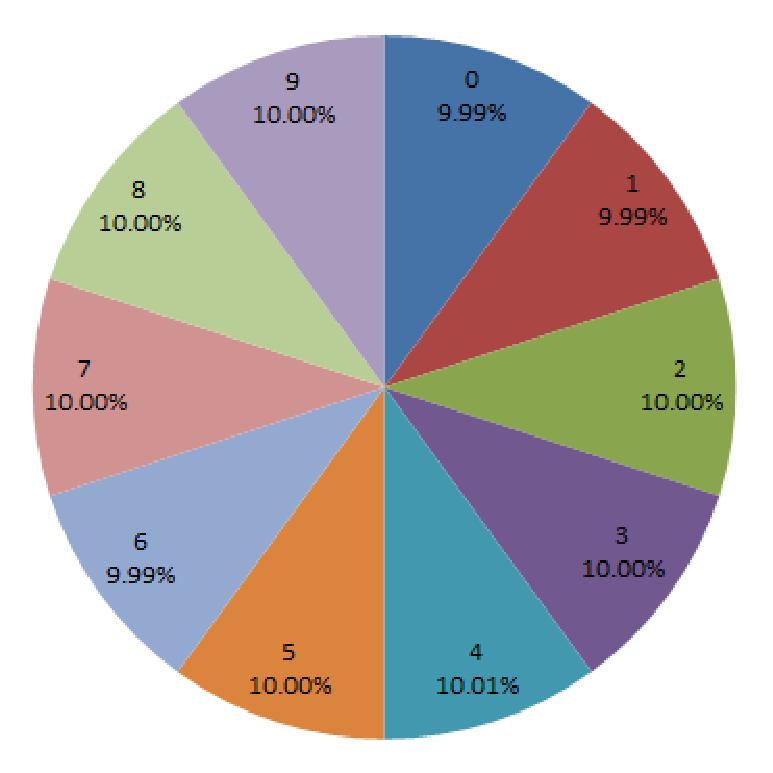
\includegraphics[width=0.9\textwidth,height=7cm]{figures/pipie}
    \end{minipage}
    \begin{minipage}[t]{0.5\linewidth}
        \centering
          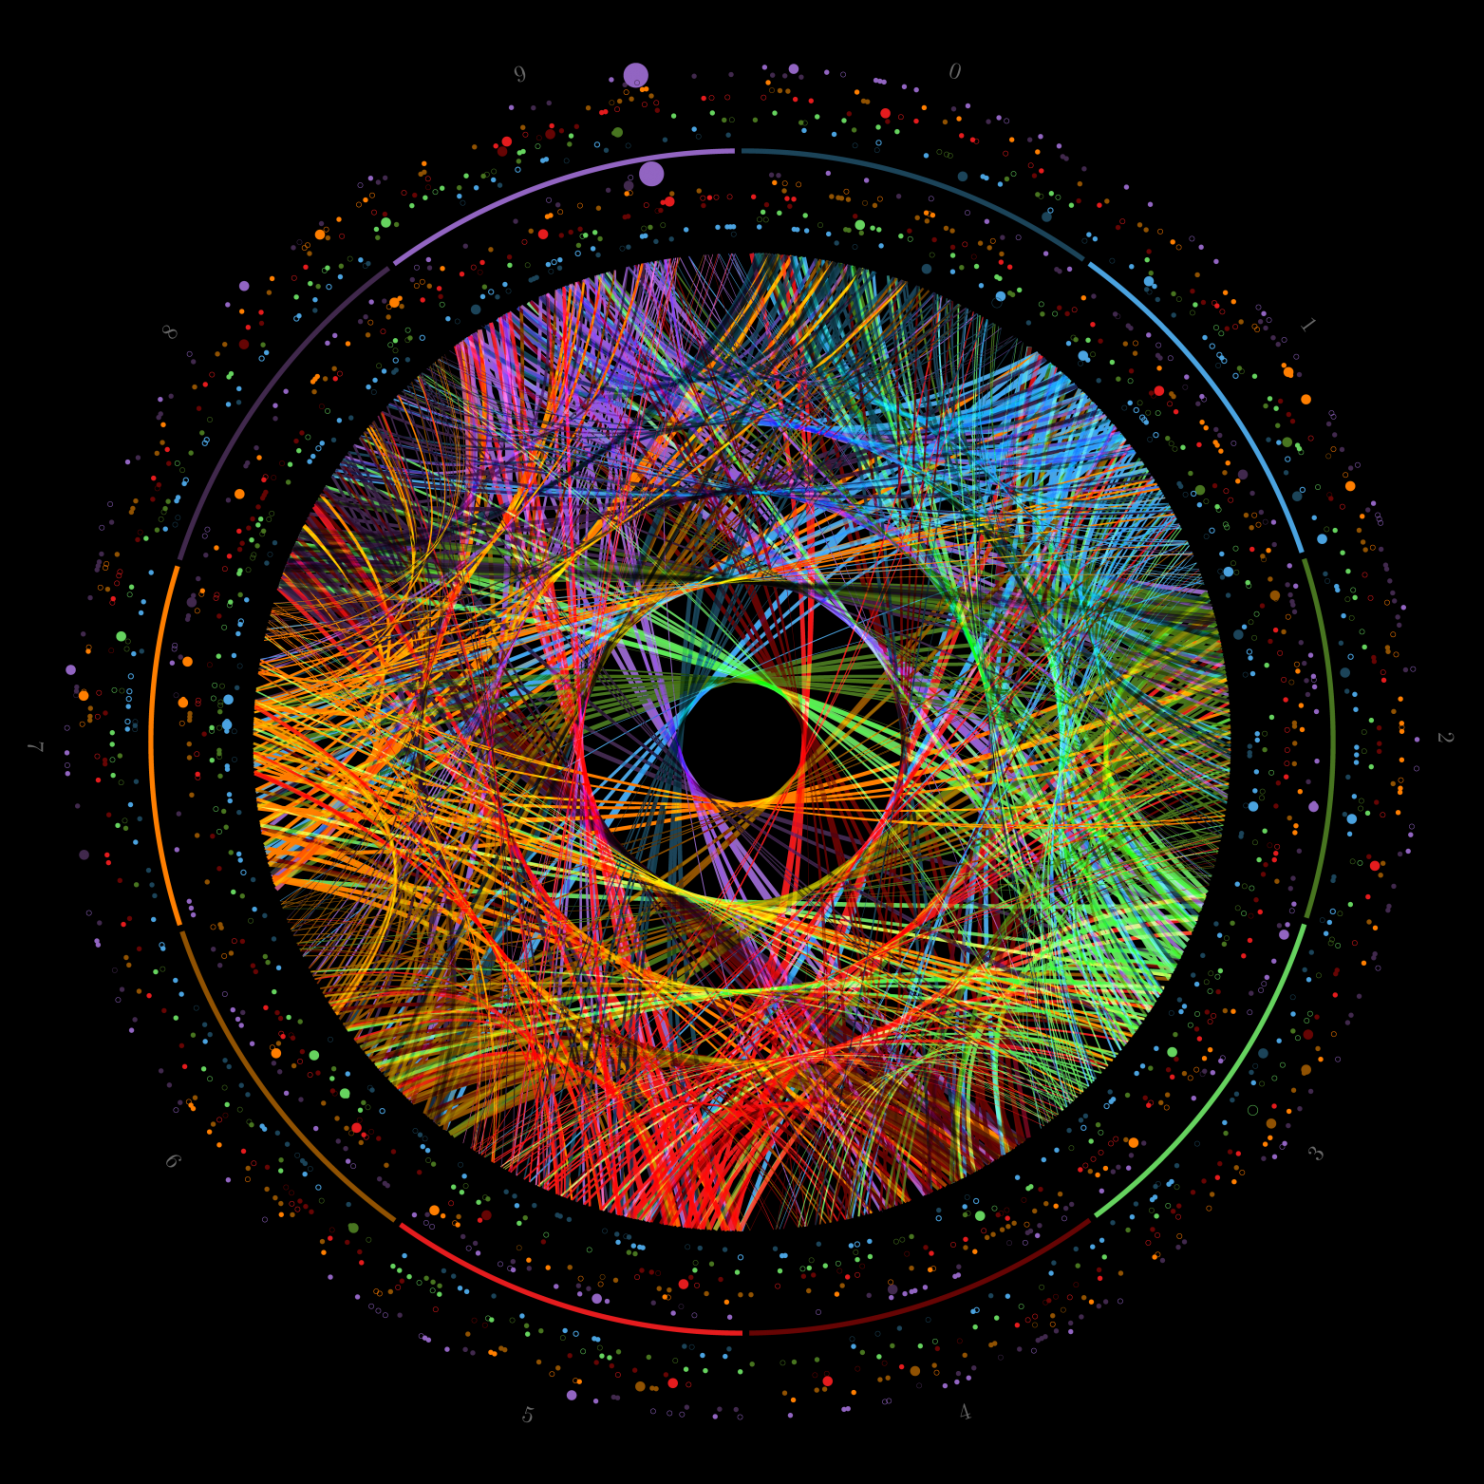
\includegraphics[width=0.9\textwidth,height=7cm]{figures/imrs-pi}
    \end{minipage}
    \caption{圆周率$\pi$值前1,000万位小数所含数字统计图(左)数字一阶转移概率矩阵图(右)}\label{fig:pipie}
\end{figure}

目前,我们还无法完全从理论上证明$\pi$的正则性,根据统计结果数字基本服从均匀分布
\[
    P_i \approx \frac{1}{10} = 0.1, i = 0, 1,\ldots,9,
\]
数值计算几乎可以肯定$\pi$就是一个正则数。如果将每个数字当作一个状态,我们利用$\pi$小数部分相邻数字建立各状态之间的\textbf{一阶转移概率矩阵}$A=(a_{ij})_{10\times 10}$,如图\ref{fig:pipie}(右):
\[
A=
\begin{pmatrix}
    0.0997 & 0.1001 & 0.1002 & 0.0997 & 0.1003 & 0.1000 & 0.0995 & 0.0996 & 0.1009 & 0.0999\\
    0.1005 & 0.0997 & 0.0997 & 0.1003 & 0.1003 & 0.0997 & 0.0997 & 0.0997 & 0.1001 & 0.1001\\
    0.1001 & 0.1003 & 0.1000 & 0.0999 & 0.1000 & 0.1000 & 0.1001 & 0.1003 & 0.0997 & 0.1005\\
    0.1001 & 0.0998 & 0.0994 & 0.1006 & 0.1001 & 0.1000 & 0.1001 & 0.0997 & 0.1001 & 0.1007\\
    0.1003 & 0.1003 & 0.1003 & 0.0998 & 0.1000 & 0.1002 & 0.1004 & 0.1004 & 0.1001 & 0.1000\\
    0.1002 & 0.1002 & 0.0999 & 0.0998 & 0.1001 & 0.1005 & 0.1000 & 0.1005 & 0.0996 & 0.1002\\
    0.0998 & 0.0996 & 0.1007 & 0.1001 & 0.1005 & 0.1000 & 0.1000 & 0.0997 & 0.0999 & 0.0997\\
    0.0994 & 0.1005 & 0.1001 & 0.1005 & 0.1000 & 0.1001 & 0.1001 & 0.1003 & 0.0998 & 0.1000\\
    0.1000 & 0.0998 & 0.1003 & 0.1000 & 0.1001 & 0.1004 & 0.1003 & 0.1003 & 0.0998 & 0.0994\\
    0.0999 & 0.0997 & 0.1003 & 0.0998 & 0.1004 & 0.1000 & 0.0997 & 0.1003 & 0.1004 & 0.1001
\end{pmatrix}
\]
转移矩阵的每一项表示一个状态转移概率
\[
    P(\pi_t = i|\pi_{t+1} = j)\approx 0.1,~~~i,j = 0,1,2,\ldots,9,
\]
每个状态都是近似于随机跳转。
\end{example}

\begin{definition}[二项分布]
如果记$A$为一次成功的伯努利实验,$p$为事件$A$发生的概率,$X$为$n$重伯努利实验中成功的次数,则$X$的可能取值为$0,1,\ldots,n$,随机变量$X$的分布列为
\begin{equation}
    P(X=k) = \binom{n}{k} p^k (1-p)^{n-k}
\end{equation}
则称$X$服从\textbf{二项分布}(Binomial Distribution),写作$X\sim B(n,p)$。当$n=1$时,则称$X$服从\textbf{两点分布},或称\textbf{$0-1$分布}:
\begin{equation}
    P(X=k) = p^k (1-p)^{1-k}, \quad k = 0, 1
\end{equation}
\end{definition}

\begin{definition}[几何分布]
如果记$A$为一次成功的伯努利实验,$p$为事件$A$发生的概率,$X$为重复伯努利实验直至事件$A$发生所需的实验次数,则$X$的可能取值为$1,\ldots,n$,随机变量$X$ 的分布列为
\begin{equation}
    P(X=k) = (1-p)^{k-1} p,\quad k = 1,2,\ldots
\end{equation}
则称$X$服从\textbf{几何分布}(Geometric Distribution),写作$X\sim \mathrm{Geo}(p)$。
\end{definition}

\begin{theorem}[几何分布的无记忆性]
假设$X\sim \mathrm{Geo}(p)$,则对任意正整数$m$与$n$,都有
\begin{equation}
    P(X > m + n | X > m) = P(X > n).
\end{equation}
\end{theorem}

\begin{definition}[负二项分布]
如果记$A$为一次成功的伯努利实验,$p$为事件$A$发生的概率,$X$为重复伯努利实验直至事件$A$出现$r$次所需的实验次数,则$X$的可能取值为$r,r+1,\ldots$,随机变量$X$ 的分布列为
\begin{equation}
    P(X=k) = \binom{k-1}{r-1} p^r (1-p)^{k-r},\quad k = r,r+1,\ldots,
\end{equation}
则称$X$服从\textbf{负二项分布}(Negative Binomial Distribution)或\textbf{Pascal分布},写作$X\sim \textrm{NB}(r, p)$。当$r=1$时,退化为几何分布。
\end{definition}

\begin{definition}[超几何分布]
假设有$N$个产品,其中有$M$个不合格产品。如果无放回地从中随机抽取$n$个,记$X$为抽取的$n$个产品中不合格的产品数目,则随机变量$X$ 的分布列为
\begin{equation}
    P(X=k) = \dfrac{\binom{M}{k}\binom{N-M}{n-k}}{\binom{N}{n}},\quad k = 1,2,\ldots, r
\end{equation}
则称$X$服从\textbf{超几何分布}(Hypergeometric Distribution),即$X\sim \mathrm{HGeo}(n, N, M)$,其中$r=\min~\{M,n\}$,并满足$M\le N$,$n\le N$,$n,M,N\in \mathbb N^{+}$。
\end{definition}

\begin{definition}[泊松分布]
如果随机变量$X$的分布列为
\begin{equation}
    P(X=k) = \frac{\lambda^k}{k!} e^{-\lambda},\quad k = 0,1,\ldots
\end{equation}
则称$X$服从\textbf{泊松分布}(Poisson Distribution),写作$X\sim \mathrm{Po}(\lambda)$。
\end{definition}

泊松分布是法国数学家Sim\'{e}on-Denis Poisson于1837年首次公开的一种离散型概率分布,它适合于刻画单位时间(或单位空间、单位产品)上随机事件发生的次数(计数过程),比如某一服务设施在一定时间内到达的人数,电话交换机接到呼叫的次数,汽车站台的候客人数,机器出现的故障数,自然灾害发生的次数,一块产品上的缺陷数,显微镜下单位分区细菌分布的数目等。

\begin{definition}[均匀分布]
如果随机变量$X$的概率密度函数为
\begin{equation}
    f(x;a, b) = \left\{
        \begin{array}{rl}
          \frac{1}{b-a}, & a < x < b, \\
          0, & else.
        \end{array}
        \right.
\end{equation}
则称$X$服从区间$(a,b)$上的\textbf{均匀分布}(Uniform Distribution),写作$X\sim U(a,b)$。
\end{definition}

\begin{definition}[指数分布]
如果随机变量$X$的概率密度函数为
\begin{equation}
    f(x;\lambda) = \left\{
        \begin{array}{rl}
          \lambda e^{-\lambda x}, & x \ge 0, \\
          0, & x < 0.
        \end{array}
        \right.
\end{equation}
则称$X$服从\textbf{指数分布}(Exponential Distribution),写作$X\sim \mathrm{Exp}(\lambda)$,$\lambda>0$为率参数(Rate Parameter),表示在单位时间间隔随机事件发生的次数。
\end{definition}

\begin{theorem}[指数分布的无记忆性]
如果$X\sim E(\lambda)$,则对任意的$s,t>0$,都有
\begin{equation}
    P(X > s+t | X>s) = P(X>t).
\end{equation}
\end{theorem}

\begin{definition}[正态分布]
如果随机变量$X$的概率密度函数为
\begin{equation}
    f(x;\mu,\sigma) = \frac{1}{\sqrt{2\pi}\sigma} \exp\{-\frac{(x-\mu)^2}{2\sigma^2}\},\quad x\in (-\infty,\infty)
\end{equation}
则称$X$服从\textbf{正态分布}(Normal Distribution),也称\textbf{高斯分布}(Gaussian Distribution)或\textbf{钟形分布}(Bell Distribution),记作$X\sim N(\mu,\sigma^2)$,参数$\mu,\sigma$ 分别表示变量的均值与标准差。当$\mu=0$,$\sigma=1$时,$X$服从\textbf{标准正态分布}$N(0,1)$。
\end{definition}

\begin{corollary}
如果随机变量$X\sim N(\mu,\sigma)$,则随机变量$Z=\frac{X-\mu}{\sigma}\sim N(0,1)$。
\end{corollary}
\begin{proof}
根据连续变量分布函数的定义,对于任意的$z\in \mathbb R$,$Z$的分布函数可表示如下:
\[
    F(z) = P(Z\le z) = P(\frac{X-\mu}{\sigma} \le z) = P(X \le \mu + z\sigma)=\int_{-\infty}^{\mu + z\sigma} f(x;\mu,\sigma) dx,
\]
展开可知
\[
    F(z) = \int_{-\infty}^{\mu + z\sigma} \frac{1}{\sqrt{2\pi}\sigma} \exp\{-\frac{(x-\mu)^2}{2\sigma^2}\} dx = \int_{-\infty}^z \frac{1}{\sqrt{2\pi}} \exp\{-\frac{x^2}{2}\} dx,
\]
直接求导可以得到相应的概率密度函数
\[
    f(z) = \frac{1}{\sqrt{2\pi}} \exp\{-\frac{x^2}{2}\},
\]
由此证得$Z\sim N(0,1)$。
\end{proof}

如果随机变量$X\sim N(\mu,\sigma)$,我们现在分析概率密度函数的凹凸性,对它求二次导数:
\[
    \frac{\partial f(x;\mu,\sigma)}{\partial x} = \frac{1}{\sqrt{2\pi} \sigma} \exp\{-\frac{(x-\mu)^2}{2\sigma^2}\} \frac{1}{\sigma^2} [\frac{(x-\mu)^2}{\sigma^2} - 1],
\]
由此可知$f(x;\mu,\sigma)$的拐点在$x=\mu \pm\sigma$处,当$|x|<\mu +\sigma$时,$f(x;\mu,\sigma)$是凹函数,否则$f(x;\mu,\sigma)$是凸函数。此外,所有正态分布都遵循一个3$\sigma$原则:$P(|x-\mu|\le \sigma) = 68.27\%$,$P(|x-\mu|\le 2\sigma) = 95.45\%$,$P(|x-\mu|\le 3\sigma) = 99.7\%$,可以方便日常估算。

\begin{theorem}
如果随机变量$X\sim N(\mu,\sigma)$,则它的数学期望是$\mu$。
\end{theorem}
\begin{proof}
利用连续随机变量的数学期望定义可知
\[
\begin{array}{lcl}
    E(X) &=& \int_{-\infty}^{+\infty}x  f(x;\mu,\sigma) dx\\
    &=& \int_{-\infty}^{+\infty}x  \frac{1}{\sqrt{2\pi}\sigma} \exp\{-\frac{(x-\mu)^2}{2\sigma^2}\} dx\\
    &=& \frac{1}{\sqrt{2\pi}\sigma} \int_{-\infty}^{+\infty} x \exp\{-\frac{(x-\mu)^2}{2\sigma^2}\} dx\\
    &=& \frac{1}{\sqrt{2\pi}} \int_{-\infty}^{+\infty} (x + \mu)\exp\{-\frac{x^2}{2}\} dx\\
    &=& \frac{\mu}{\sqrt{2\pi}} \int_{-\infty}^{+\infty} \exp\{-\frac{x^2}{2}\} dx.
\end{array}
\]
我们利用二重积分,通过极坐标变换
\[
\left\{
    \begin{array}{lcl}
        x &=& r\cos\theta,\\
        y &=& r\sin\theta,
    \end{array}
\right.
\]
简化计算:
\[
\begin{array}{lcl}
    E(X)^2 &=& \frac{\mu^2}{2\pi} \int_{-\infty}^{+\infty} \int_{-\infty}^{+\infty} \exp\{-\frac{x^2 + y^2}{2}\} dx dy\\
    &=& \frac{\mu^2}{2\pi} \int_0^{2\pi} \int_0^{+\infty} r \exp\{-\frac{r^2}{2}\} dr d\theta\\
    &=& \mu^2 [\exp\{-\frac{r^2}{2}\}_{|r=0} - \exp\{-\frac{r^2}{2}\}_{|r=+\infty}]\\
    &=& \mu^2,
\end{array}
\]
由于$E(X)>0$,则$E(X)=\mu$得证。
\end{proof}

\begin{definition}[对数正态分布]
如果随机变量$X$的概率密度函数为
\begin{equation}
    f(x;\mu,\sigma) = \frac{1}{x\sigma\sqrt{2\pi}} \exp\{-\frac{(\ln x-\mu)^2}{2\sigma^2}\},\quad x > 0
\end{equation}
则称$X$服从\textbf{对数正态分布}(Logarithmic Normal Distribution),也称\textbf{高尔顿分布}(Galton Distribution),记作$X\sim \mathrm{LN}(\mu,\sigma^2)$。
\end{definition}

\begin{theorem}
如果$X\sim \mathrm{LogN}(\mu, \sigma^2)$,则$Y=\ln X\sim N(\mu, \sigma^2)$。如果$\sigma>0$,则有\[Z=(Y-\mu)/\sigma\sim N(0,1).\]
\end{theorem}

\begin{definition}[伽马分布]
如果随机变量$X$的概率密度函数为
\begin{equation}
    f(x;\alpha,\lambda) = \left\{
    \begin{array}{cc}
        \frac{\lambda^\alpha}{\Gamma(\alpha)} x^{\alpha-1} e^{-\lambda x} & x \ge 0,\\
        0 & x < 0.
    \end{array}
    \right.
\end{equation}
则称$X$服从\textbf{伽马分布}(Gamma Distribution),记作$X\sim \mathrm{Ga}(\alpha,\lambda)$,其中$\alpha>0$为\textbf{形状参数}(Shape Parameter),$\lambda>0$为\textbf{尺度参数}(Scale Parameter),$\Gamma$ 表示如下形式的伽马函数:
\begin{equation}
    \Gamma(\alpha) = \int_0^{+\infty} x^{\alpha-1} e^{-x} dx,\quad \alpha>0.
\end{equation}
当$\alpha=1$时,伽马分布退化为指数分布,当$\alpha=n/2$,$\lambda=1/2$时,伽马分布退化为自由度为$n$的卡方分布。
\end{definition}

\begin{definition}[贝塔分布]
如果随机变量$X$的概率密度函数为
\begin{equation}
    f(x;a,b) = \left\{
    \begin{array}{rl}
        \frac{1}{B(a,b)} x^{a-1} (1- x)^{b-1}, & 0 < x < 1,\\
        0, & else.
    \end{array}
    \right.
\end{equation}
则称$X$服从\textbf{贝塔分布}(Beta Distribution),记作$X\sim \mathrm{Be}(a,b)$,其中$a,b>0$都是形状参数,$B$表示如下形式的贝塔函数:
\begin{equation}
    B(a,b) = \int_0^1 x^{a-1} (1-x)^{b-1} dx,\quad a>0,b>0.
\end{equation}
根据伽马函数的定义可知两者存在下面形式的关系:
\begin{equation}
    B(a,b) = \frac{\Gamma(a)\Gamma(b)}{\Gamma(a+b)}.
\end{equation}
当$a=b=1$时,贝塔分布退化为均匀分布$U(0,1)$。
\end{definition}

\begin{definition}[拉普拉斯分布]
如果随机变量$X$的概率密度函数为
\begin{equation}
    f(x;\eta,\theta) = \frac{1}{2\theta} \exp\{-\frac{|x-\eta|}{\theta}\},\quad x \in (-\infty,\infty)
\end{equation}
则称$X$服从\textbf{拉普拉斯分布}(Laplace Distribution),也称\textbf{双指数分布},记作$X\sim \mathrm{La}(\eta,\theta)$,参数$\eta,\theta$分别表示随机变量$X$ 的均值与标准差。
\end{definition}

1901年,Josiah Gibbs在研究统计力学时发现一种新的分布模型:\textbf{玻尔兹曼分布}(Boltzmann Distribution),也称\textbf{Gibbs分布}。在统计和机器学习领域,玻尔兹曼分布又称作\textbf{对数线性模型}(Log-linear Model)。
\begin{definition}[玻尔兹曼分布]
在一个封闭系统中,当系统温度为$T$时,处于状态$S_i$,能量为$E_i$的粒子所占比例$N_i/N$
\begin{equation}
    \frac{N_i}{N} = \frac{1}{Z(T)} g_i \exp\{-\frac{E_i}{\kappa T}\}
\end{equation}
其中,$g_i$表示拥有能量$E_i$的状态数目,$Z(T)$是标准化因子,在统计力学中称\textbf{配分函数(Partition Function)}
\begin{equation}
    Z(T) = \sum\limits_i g_i \exp\{-\frac{E_i}{\kappa T}\}
\end{equation}
而$N$表示系统中粒子总数$N=\sum\limits_i N_i$。
\end{definition}

\begin{theorem}[卷积公式]
假设$X$与$Y$是两个相互独立的连续型随机变量,两变量的概率密度函数分别是$f_X(x)$和$f_Y(y)$,则两者之和$Z=X+Y$的概率密度函数为
\begin{equation}
    f_Z(z) = \int_{-\infty}^{+\infty} f_X(z-y) f_Y(y) dy
\end{equation}
也称概率密度函数$f_X(x)$和$f_Y(y)$的\textbf{卷积}(Convolution),可视作\textbf{移动平均}的推广。
\end{theorem}

\begin{theorem}[正态分布的可加性]
假设$X\sim N(\mu_1,\sigma_1^2)$,$Y\sim N(\mu_2,\sigma_2^2)$,且相互独立,则$Z=X+Y\sim N(\mu_1+\mu_2,\sigma_1^2 +\sigma_2^2)$。
\end{theorem}

\section{概率不等式}%Probability Inequalities
\subsection{集中不等式}
集中不等式(Concentration Inequalities)刻画了一个随机变量在给定取值附近集中分布的状况。比如,大数定律描述了一系列独立同分布随机变量的均值在概率上趋近于它们的数学期望。当变量数目逐渐增大,变量均值会集中在变量期望附近。

\begin{theorem}[Markov不等式]
假设$X$是非负随机变量,存在期望$E(X)$。对于任意的实数$t>0$,都有
\begin{equation}
    P(X\ge t) \le \frac{E(X)}{t}
\end{equation}
\end{theorem}
\begin{proof}
记变量
\begin{equation}
    I = \left\{
        \begin{array}{ll}
          1 & X\ge t \\
          0 & X < t
        \end{array}
    \right.
\end{equation}
由于$I\le X/t$,两边同时取期望,则有$P(X\ge t)=E(I) \le E(X)/t$成立。
\end{proof}

\begin{theorem}[Mill不等式]
假设随机变量$X\sim N(0,1)$,则对任意的实数$t>0$,都有
\[
    P(|X|>t) \le \sqrt{\frac{2}{\pi}} \frac{e^{-t^2/2}}{t}.
\]
\end{theorem}
\begin{proof}
根据定义则有
\[
\begin{array}{lcl}
    P(|X|>t) &=& \int_{-\infty}^{-t} f(x) dx + \int_t^{+\infty} f(x) dx \\
    &=& 2\int_t^{+\infty} \frac{1}{\sqrt{2\pi}} e^{-x^2/2} dx\\
    &\le& \sqrt{\frac{2}{\pi}} \int_t^{+\infty} \frac{x}{t} e^{-x^2/2} dx\\
    &=& \sqrt{\frac{2}{\pi}} \frac{e^{-t^2/2}}{t}.
\end{array}
\]
证毕。
\end{proof}

\begin{theorem}[Chebyshev不等式]
假设随机变量$X$存在期望$\mu = E(X)$和方差$\sigma^2 = \var(X)$,则对任意的实数$t>0$,都有
\begin{equation}
    P(|X-\mu|\ge t) \le \frac{\sigma^2}{t^2}
\end{equation}
\end{theorem}
\begin{proof}
由于$(X-\mu)^2$是非负随机变量,由Markov不等式可知
\begin{equation}
    P((X-\mu)^2\ge t^2) \le \frac{E[(X-\mu)^2]}{t^2} = \frac{\sigma^2}{t^2}
\end{equation}
等价于
\begin{equation}
    P(|X-\mu|\ge t) \le \frac{\sigma^2}{t^2}
\end{equation}
若记$Z = (X-\mu)/\sigma$,则有
\begin{equation}
    P(|Z|\ge 2) \le \frac{1}{4}, ~~P(|Z|\ge 3) \le \frac{1}{9}
\end{equation}
Chebyshev不等式并未限定随机变量分布的具体形式,存在广泛应用。
\end{proof}

\begin{theorem}[Chernoff界]
如果随机变量$X$存在矩母函数$\psi$,则对任意的$t$,都有
\[
    P(X\ge t) \le \min\limits_{s>0} \frac{\psi(s)}{e^{st}}.
\]
\end{theorem}
\begin{proof}
对于任意的$s>0$,都有
\[
    P(X\ge t) = P(e^{sX} \ge e^{st}),
\]
根据Markov不等式可得
\[
    P(e^{sX} \ge e^{st}) \le e^{-st} E(e^{sX} = \frac{\psi(s)}{e^{st}}.
\]
由于$s$的任意性,从而可得
\[
    P(X\ge t) \le \min\limits_{s>0} \frac{\psi(s)}{e^{st}}.
\]
\end{proof}

\begin{lemma}[Hoeffding法则]
假设$X$是$[a,b]$上的随机变量,并且$E(X)=0$,则对任意实数$t>0$有
\begin{equation}
   \psi(t) = E[e^{tX}] \le e^{t^2(b-a)^2/8}
\end{equation}
\end{lemma}
\begin{proof}
由于$e^{tX}$是凸函数,则由Jensen不等式可知
\begin{equation}
  e^{tX} \le \frac{b-X}{b-a} e^{ta} + \frac{X-a}{b-a} e^{tb}
\end{equation}
两边同时取期望,则有
\begin{equation}
  E[e^{tX}] \le \frac{E(b-X)}{b-a} e^{ta} + \frac{E(X-a)}{b-a} e^{tb}
\end{equation}
由于$E(X)=0$,所以
\begin{equation}
  E[e^{tX}] \le \frac{b}{b-a} e^{ta} - \frac{a}{b-a} e^{tb} \triangleq e^{\phi(t)}
\end{equation}
其中,$\phi(t)=\ln\big(\frac{b}{b-a} e^{ta} - \frac{a}{b-a} e^{tb}\big)$,我们只要证明$\phi(t)\le t^2(b-a)^2/8$即可。

由于
\begin{eqnarray}
    \phi'(t) &=& \frac{ab}{b e^{ta} - a e^{tb}} (e^{ta} - e^{tb}) \\
    \phi''(t) &=& \frac{(1-\alpha) e^{-t(b-a)}}{[(1-\alpha) e^{-t(b-a)} + \alpha]} \times \frac{\alpha}{[(1-\alpha) e^{-t(b-a)} + \alpha]} \times (b-a)^2 \le \frac{1}{4} (b-a)^2,
    \end{eqnarray}
其中,$\alpha=\frac{-a}{b-a}$。根据Taylor展开式,可知存在$\theta\in[0,t]$,满足
\begin{equation}
  \phi(t) = \phi(0) + t\phi'(0) + \frac{1}{2} t^2 \phi''(\theta) \le \frac{1}{8} t^2(b-a)^2
\end{equation}
则命题得证。
\end{proof}

\begin{theorem}[Hoeffding不等式]
假设$X_1,\ldots, X_n$是相互独立的随机变量,且$X_i\in[a_i,b_i], i =1,\ldots,n$。记$S_n=\sum\limits_i X_i$,对任意的$\epsilon>0$则有
\begin{equation}
    P(|S_n-E(S_n)| \ge \epsilon) \le \exp\bigg\{-\frac{2\epsilon^2}{\sum\limits_i (b_i-a_i)^2}\bigg\}.
\end{equation}

\begin{proof}
由于$P(S_n-E(S_n) \ge \epsilon) = P(e^{S_m-E(S_m)} \ge e^\epsilon)$,根据Markov不等式,则有
\begin{equation}
    P(e^{t[S_n-E(S_n)]} \ge e^{t\epsilon}) \le \frac{E[e^{t
    [S_n-E(S_n)]}]}{e^{t\epsilon}} = \frac{E[\prod\limits_i e^{t(X_i-E(X_i))}]}{e^{t\epsilon}}
\end{equation}
由$X_1,X_2,\ldots, X_n$的独立性和Hoeffding法则有
\begin{equation}
  \frac{E[\prod\limits_i e^{t(X_i-E(X_i))}]}{e^{t\epsilon}} = \frac{\prod\limits_i E[e^{t(X_i-E(X_i))}]}{e^{t\epsilon}} \le \frac{\prod\limits_i e^{t^2(b_i-a_i)^2/8}}{e^{t\epsilon}} = \frac{e^{t^2 \sum\limits_i (b_i-a_i)^2/8}}{e^{t\epsilon}}
\end{equation}
只要取$t = 4\epsilon/\sum\limits_i (b_i-a_i)^2$,则
\begin{equation}
    P(S_m-E(S_m) \ge \epsilon) \le \exp\bigg\{-\frac{2\epsilon^2}{\sum\limits_i (b_i-a_i)^2}\bigg\},
\end{equation}
同理可证
\begin{equation}
    P(S_m-E(S_m) \le -\epsilon) \le \exp\bigg\{-\frac{2\epsilon^2}{\sum\limits_i (b_i-a_i)^2}\bigg\},
\end{equation}
命题得证。
\end{proof}
\end{theorem}
Hoeffding不等式从本质上说明一组独立随机变量的均值离开其期望值的可能性以指数形式衰减,即有
\[
    P(|\bar X - E (\bar X)| \ge \epsilon) \le \exp\bigg\{-\frac{2 n^2 \epsilon^2}{\sum\limits_i (b_i-a_i)^2}\bigg\}\rightarrow 0~~~(n\rightarrow \infty).
\]
如果每个随机变量都有一个较小的方差,我们可以推导出更紧的概率界。

\begin{lemma}[Azuma法则]
假设随机变量$X$和$Y$满足$E(X|Y)=0$,且存在函数$f$和常数$c$使得不等式$f(Y)\le X \le f(Y)+c$成立,则对任意的实数$t>0$都有
\begin{equation}
    E(e^{tX}|Y) \le \exp\{\frac{t^2c^2}{8}\}.
\end{equation}

\end{lemma}
\begin{proof}
根据Hoeffding法则与条件期望的相加性,命题易证。我们令$a = f(Y)$,$b = f(Y) + c$,于是$b - a = c$。由于$e^{tX}$是凸函数,则由Jensen不等式可知
\begin{equation}
  e^{tX} \le \frac{b-X}{b-a} e^{ta} + \frac{X-a}{b-a} e^{tb}
\end{equation}
由$E(X|Y)=0$和条件期望的线性相加性可得:
\begin{equation}
    E(e^{tX}|Y) \le E\bigg(\frac{b-X}{b-a} e^{ta} + \frac{a-X}{b-a}e^{tb} |Y\bigg) = \frac{b e^{ta}-a e^{tb}}{b-a}.
\end{equation}
之后证明与Hoeffding不等式的证明完全一致,命题得证。
\end{proof}

\begin{definition}[鞅差序列]
假设$X_1,X_2,\ldots$和$Y_1, Y_2,\ldots$是两个随机变量序列,如果对于任意$i>0$,$Y_i$是$X_1,X_2,\ldots,X_i$的函数,且有
\[
    E(Y_{i+1}|X_1,X_2,\ldots,X_i) = 0,
\]
则称$Y_1, Y_2,\ldots$是关于$X_1,X_2,\ldots$的\textbf{鞅差序列}。
\end{definition}

\begin{theorem}[Azuma不等式]
假设$Y_1, Y_2,\ldots$是关于$X_1,X_2,\ldots$的鞅差序列,如果对于任意的$i>0$,都存在常数$c_i$和关于$X_1,X_2,\ldots,X_{i-1}$的随机变量$Z_i$,并满足不等式
$Z_i\le Y_i \le Z_i + c_i$,那么对任意的$\epsilon>0$和正整数$n$都有
\[
    P(|\sum\limits_n Y_i| \ge \epsilon) \le \exp\big\{-\frac{2\epsilon^2}{\sum\limits_i c_i^2}\big\}.
\]
\end{theorem}

\begin{proof}
假设$S_k=\sum\limits_{i=1}^k Y_i$,$1\le k\le n$,则对任意的实数$t>0$,由Markov不等式易知
\[
    P(S_n\ge \epsilon) = P(tS_n\ge t\epsilon) \le \frac{E e^{tS_n}}{e^{t\epsilon}} = \frac{E (e^{tS_{n-1}} e^{tY_n})}{e^{t\epsilon}},
\]
并且$e^{tS_{n-1}}$是$X_1,X_2,\ldots,X_{n-1}$的函数,由条件期望的性质可得
\[
    E (e^{tS_{n-1}} e^{tY_n}) = E\big(e^{tS_{n-1}} E(e^{tY_n}|X_1,X_2,\ldots, X_{n-1})\big).
\]
根据Azuma法则可知$E(e^{tY_n}|X_1,X_2,\ldots, X_{n-1}) \le e^{t^2 c_n^2/8}$,于是有
\[
    P(S_n\ge \epsilon) \le \frac{E (e^{tS_{n-1}} e^{tY_n})}{e^{t\epsilon}} \le \frac{E (e^{tS_{n-1}} e^{t^2 c_n^2/8})}{e^{t\epsilon}} \le \cdots \le \frac{e^{t^2 \sum\limits_i c_i^2/8}}{e^{t\epsilon}}.
\]
如果取$t=4\epsilon /\sum\limits_i c_i^2$,可得
\[
    P(\sum\limits_i Y_i \ge \epsilon) \le \exp\big\{-\frac{2\epsilon^2}{\sum\limits_i c_i^2}\big\},
\]
同理可证
\[
    P(\sum\limits_i Y_i \le -\epsilon) \le \exp\big\{-\frac{2\epsilon^2}{\sum\limits_i c_i^2}\big\},
\]
命题得证。
\end{proof}

\begin{theorem}[McDiarmid不等式]
假设$X_1,\ldots, X_n\in \mathcal X$是相互独立的随机变量且存在实数$c_1,\ldots,c_n>0$和函数$f:\mathcal X^n \mapsto \mathbb R$,使得对于任意的$x_1,\ldots,x_i, \ldots, x_n,x'_i$都有
\[
   |f(x_1,\ldots,x_i,\ldots,x_n) - f(x_1,\ldots,x'_i,\ldots,x_n)| \le c_i,
\]
设$f(S)=f(X_1,X_2,\ldots, X_n)$,那么对于任意的$\epsilon>0$和正整数$n$有
\begin{equation}
    P(|f(S) - E(f(S))|\ge \epsilon) \le \exp\big\{-\frac{2\epsilon^2}{\sum\limits_i c_i^2}\big\}.
\end{equation}
\end{theorem}
\begin{proof}
我们记随机变量$Y=f(S)-E(f(S))$和随机变量序列$\{Y_k\}_{k=1}^n$:
\begin{eqnarray}
  \nonumber Y_1 &=& E(Y|X_1) - E(Y), \\
  \nonumber \vdots && \\
  \nonumber Y_k &=& E(Y|X_1, X_2,\ldots,X_k) - E(Y|X_1,X_2,\ldots, X_{k-1}),~~~k=2,3,\ldots,n,
\end{eqnarray}
显然$\sum\limits_k Y_k = E(Y|X_1, X_2,\ldots,X_n) - E(Y)$,又$E(Y)=0$,而
\[
\begin{array}{lcl}
    E(Y|X_1, X_2,\ldots,X_n) &= &E(f(S)-E(f(S))|X_1, X_2,\ldots,X_n)\\
     &=& E(f(S)|X_1, X_2,\ldots,X_n) - E(E(f(S))|X_1, X_2,\ldots,X_n),
\end{array}
\]
由于$f(S)$是$X_1,X_2,\ldots, X_n$的一个函数,$E(f(S))$是个标量,所以有
\[
    \sum\limits_k Y_k = E(Y|X_1, X_2,\ldots,X_n) = f(S) - E(f(S)) = Y.
\]
此外,根据条件期望的性质可知
\[
    E(Y|X_1,\ldots,X_k) = E(E(Y|X_1,\ldots,X_k)|X_1,\ldots,X_{k-1}),
\]
于是
\begin{eqnarray}
  \nonumber E(Y_k|X_1,\ldots,X_{k-1}) &=& E(E(Y|X_1, X_2,\ldots,X_k) - E(Y|X_1,X_2,\ldots, X_{k-1})|X_1,\ldots,X_{k-1}) \\
  \nonumber &=&  E(E(Y|X_1, X_2,\ldots,X_k)|X_1,\ldots,X_{k-1}) - \\
  \nonumber &&   E(E(Y|X_1,X_2,\ldots, X_{k-1})|X_1,\ldots,X_{k-1})\\
  \nonumber &=&  E(Y|X_1,\ldots,X_k) - E(Y|X_1,X_2,\ldots, X_{k-1})\\
  \nonumber &=&  0.
\end{eqnarray}
所以序列$Y_1,Y_2,\ldots, Y_n$是关于$X_1,X_2,\ldots, X_n$的鞅差序列。由于$E(f(S))$是个标量,则
\[
    Y_k = E(Y|X_1,\ldots,X_k) - E(Y|X_1,\ldots,X_{k-1}) = E(f(S)|X_1,\ldots,X_k) - E(f(S)|X_1,\ldots,X_{k-1}),
\]
我们定义$U_k$和$V_k$:
\begin{eqnarray}
  \nonumber U_k &=& \sup\limits_X E (f(S) |X_1,\ldots,X_{k-1},X ) - E (f(S) |X_1,\ldots,X_{k-1}), \\
  \nonumber V_k &=& \inf\limits_X E (f(S) |X_1,\ldots,X_{k-1},X ) - E (f(S) |X_1,\ldots,X_{k-1}),
\end{eqnarray}
可知$U_k-V_k=\sup\limits_{X, X'} E (f(S) |X_1,X_2,\ldots,X_{k-1},X ) - E (f(S) |X_1,X_2,\ldots,X_{k-1},X')\le c_k$,从而有不等式
$V_k\le Y_k \le U_k \le V_k + c_k$,由Azuma不等式可得:
\[
    P(f(S) - E(f(S)) \ge \epsilon) \le \exp\big\{-\frac{2\epsilon^2}{\sum\limits_i c_i^2}\big\},
\]
同理可证
\[
    P(f(S) - E(f(S)) \le -\epsilon) \le \exp\big\{-\frac{2\epsilon^2}{\sum\limits_i c_i^2}\big\}.
\]
证毕。
\end{proof}
如果取$f(x_1,x_2,\ldots, x_n) = \sum\limits_i x_i$,可以看出Hoeffiding不等式是McDiarmid不等式的一个特例。

\begin{theorem}[Bennett不等式和Bernstein不等式]
假设随机变量$X_1,X_2,\ldots,X_n$是独立的随机变量,且$X_i\le c$,$E (X_i) = 0$,$E (X_i^2) = \sigma_i^2$。如果记$\sigma^2 = \sum\limits_i \sigma_i^2/n$,那么对任意的实数$\epsilon>0$有
\begin{eqnarray}
  P\big(\sum\limits_i X_i/n \ge \epsilon\big) &\le & \exp\bigg\{-\frac{n\sigma^2}{c^2}f(\frac{\epsilon c}{\sigma^2})\bigg\}, \\
  P\big(\sum\limits_i X_i/n \ge \epsilon\big) &\le & \exp\bigg\{-\frac{n\epsilon^2}{2\sigma^2 + 2\epsilon c/3}\bigg\}.
\end{eqnarray}
其中函数$f(x)=(1+x)\log(1+x)-x$,两个不等式分别称作Bennett不等式和Bernstein不等式。
\end{theorem}

\begin{proof}
对任意实数$t>0$,由Markov不等式和$X_1,X_2,\ldots,X_n$的独立性易知:
\begin{equation}
    P\big(\sum\limits_i X_i/n \ge \epsilon\big) = P\big(e^{t\sum\limits_i X_i} \ge e^{n\epsilon t}\big) \le \frac{E(e^{t\sum\limits_i X_i})}{e^{n\epsilon t}} = \frac{\prod\limits_i E(e^{tX_i})}{e^{n\epsilon t}}.
\end{equation}
我们定义$\mathbb R$上的一个连续函数$g(x)$:
\[
g(x)=\left\{
\begin{array}{rl}
\dfrac{e^x-1-x}{x^2}, & x\in \mathbb R\setminus \{0\},\\
\dfrac{1}{2}, & x = 0.
\end{array}
\right.
\]
可以证明$g(x)$是单调递增函数,那么给定$t>0$,对于任意的$x\le c$都有$g(tx) \le g(tc)$,即是说
\[
    e^{tx} \le 1 + tx + \frac{x^2}{c^2}(e^{tc} - 1 -tc),
\]
根据期望的线性性质,以及$E(X_i)=0$和$E(X_i^2)=\sigma_i^2$可得
\[
    E(e^{tX_i}) \le E\big[1 + tX_i + \frac{X_i^2}{c^2}(e^{tc} - 1 -tc)\big] = 1 + \frac{\sigma_i^2}{c^2}(e^{tc} - 1 -tc) \le e^{\sigma_i^2(e^{tc}-1-tc)/c^2},
\]
于是
\[
    P\big(\sum\limits_i X_i/n \ge \epsilon\big) \le \frac{\prod\limits_i E(e^{tX_i})}{e^{n\epsilon t}} \le \frac{\prod\limits_i e^{\sigma_i^2(e^{tc}-1-tc)/c^2}}{e^{n\epsilon t}} = \frac{e^{\sigma^2(e^{tc}-1-tc)/c^2}}{e^{n\epsilon t}}.
\]
如果取$t=\log(1+(\epsilon c)/\sigma^2)/c$,可以证得Bennett不等式。

我们引入函数
\[
    h(x) = f(x) - \frac{3}{2} \frac{x^2}{x+3},
\]
可以证明$h(x)$是单调递增函数,且$h(0)=0$,所以$h(x)\ge 0$,即$f(x) \ge \frac{3}{2} \frac{x^2}{x+3}$,于是可以证得Bernstein不等式成立。
\end{proof}
这些形式相似的概率不等式描述了一组独立随机变量的均值偏离其期望的概率。如果将每个随机变量看做是某个样本的分类情况,那么通过这些不等式我们可以直接推得泛化误差偏离经验误差的概率,也是统计学习理论分析的基本思路。

\subsection{大数定律}
\textbf{大数定律}(Law of Large Numbers)讨论随机变量和的平均值的收敛情况,是数理统计学中\textbf{参数估计}的理论基础。\textbf{中心极限定理}(Central Limit Theorem)是讨论随机变量序列部分和的分布渐进收敛于正态分布的一组定理,是数理统计学中\textbf{误差分析}的理论基础,指出大量随机变量近似服从正态分布的条件。大数定律和中心极限定理都涉及到随机变量序列的收敛性分析,比如大数定律涉及到\textbf{依概率收敛}(Convergence in Probability),中心极限定理涉及到\textbf{依分布收敛}(Convergence in Distribution)。这些极限定理(Limit Theorems)是概率论的重要内容和数理统计学的基石之一
\footnote{18$\sim$19世纪,极限定理一直是概率论研究的中心课题。Bernoulli大数定律是第一个从数学上被严格证明的概率论定律,由Bernoulli在其1713年出版的《推测术》中详细给出,而“大数定律”这个名称是由Poisson在1837年给出。美籍匈牙利数学家George Polya是第一个在论著中使用“中心极限定理”(1920)术语的人,他还首创了术语“随机游走”(Random Walk,1921)。最初的中心极限定理是关于$n$重Bernoulli试验的,1716年法国数学家Abraham de Moivre讨论了$p=1/2$的情形,随后Pierre-Simon Laplace将其推广到$0<p<1$的情形。从19世纪中叶到20世纪初,一大批著名的前苏联数学家运用严格的、强有力的数学分析工具,如傅里叶变换等,将Bernoulli大数定律、De Moivre-Laplace中心极限定理推广到一般随机变量序列部分和的情形。}。

\begin{definition}[依概率收敛]
假设$\{X_n, n\in \mathbb N\}$是一个随机变量序列,$X$是一个随机变量。如果对任意的$\epsilon>0$,都有
\[
    \lim\limits_{n\rightarrow +\infty} P(|X_n-X|<\epsilon) = 1,
\]
则称$\{X_n, n\in \mathbb N\}$\textbf{依概率收敛}于$X$,记作$X_n \stackrel{P}{\longrightarrow} X$。
\end{definition}

\begin{definition}[几乎处处收敛]
假设$\{X_n, n\in \mathbb N\}$是一个随机变量序列,$X$是一个随机变量。如果
\[
    P(\lim\limits_{n\rightarrow +\infty} X_n = X) = 1,
\]
则称$\{X_n, n\in \mathbb N\}$\textbf{几乎处处收敛}(Almost Surely Converge)或\textbf{以概率1收敛}(Converge with Probability One)于$X$,记作$X_n \stackrel{a.s}{\longrightarrow} X$。
\end{definition}

\begin{definition}[依分布收敛]
假设$\{X_n, n\in \mathbb N\}$是一个随机变量序列,$X$是一个随机变量,$X_n$的分布函数是$F_n(x)$,$X$的分布函数是$F(x)$。如果对$F(x)$的任意连续点$x$,都有
\[
    \lim\limits_{n\rightarrow +\infty} F_n(x) = F(x),~~~n\in \mathbb N,
\]
则称$\{F_n(x), n\in \mathbb N\}$\textbf{弱收敛}于$F(x)$,记作$F_n(x) \stackrel{W}{\longrightarrow} X$,也称$\{X_n, n\in \mathbb N\}$\textbf{依分布收敛}于$X$,记作$X_n \stackrel{L}{\longrightarrow} X$。
\end{definition}

\begin{theorem}[Bernoulli大数定律]
设$\{X_n,n\in \mathbb N\}$是独立的两点分布随机变量序列,$P(X_n=1)=p$,$P(X_n=0)=1-p$,$0<p<1$,记序列前$n$个随机变量的部分和
\[
    S_n = \sum\limits_{i=1}^n X_i,
\]
则$S_n/n\stackrel{P}{\longrightarrow} p$,对任意的$\epsilon>0$都有
\[
   \lim\limits_{n\rightarrow +\infty} P(|\frac{S_n}{n} - p|<\epsilon) = 1.
\]
\end{theorem}
\begin{proof}
由于$S_n\sim B(n,p)$,则$S_n/n$的数学期望和方差都存在,且$E(S_n/n)=p$,$\var(S_n/n)=p(1-p)/n$。根据Chebyshev不等式,对任意的$\epsilon>0$,都有
\[
    1\ge  P(|\frac{S_n}{n} - p|< \epsilon) \ge 1- \frac{\var(S_n/n)}{\epsilon^2} = 1- \frac{p(1-p)}{n\epsilon^2},
\]
当$n\rightarrow +\infty$时,不等式右端趋于$1$:
\[
    \lim\limits_{n\rightarrow +\infty} P(|\frac{S_n}{n} - p|<\epsilon) = \lim\limits_{n\rightarrow +\infty} P(|\frac{1}{n} \sum\limits_{i=1}^n X_i - \frac{1}{n} \sum\limits_{i=1}^n E(X_i)|<\epsilon) = 1,
\]
命题得证。
\end{proof}

\begin{definition}
设$\{X_n, n\in \mathbb N\}$是一个随机变量序列,如果对任意的$\epsilon>0$,都有
\[
    \lim\limits_{n\rightarrow +\infty} P(|\frac{1}{n} \sum\limits_{i=1}^n X_i - \frac{1}{n} \sum\limits_{i=1}^n E(X_i)|<\epsilon) = 1,
\]
则称$\{X_n, n\in \mathbb N\}$服从大数定律。
\end{definition}

\begin{theorem}[Chebyshev大数定律]
设$\{X_n, n\in \mathbb N\}$是一个独立随机变量序列,如果每个随机变量$X_n$的方差存在,且有共同的上界,即$\var(X_n)\le c$,则$\{X_n, n\in \mathbb N\}$服从大数定律。
\end{theorem}

\begin{proof}
由于$\{X_n, n\in \mathbb N\}$相互独立,则部分和均值方差
\[
    \var(\frac{1}{n} \sum\limits_{i=1}^n X_i) = \frac{1}{n^2} \sum\limits_{i=1}^n \var(X_i) \le \frac{c}{n}.
\]
根据Chebyshev不等式,对任意的$\epsilon>0$都有
\[
    \lim\limits_{n\rightarrow +\infty} P(|\frac{1}{n} \sum\limits_{i=1}^n X_i - \frac{1}{n} \sum\limits_{i=1}^n E(X_i)| < \epsilon) \ge  1 - \frac{\var(\sum\limits_{i=1}^n X_i/n)}{\epsilon^2} \ge 1 - \frac{c}{n\epsilon^2}.
\]
当$n\rightarrow +\infty$时,有
\[
    \lim\limits_{n\rightarrow +\infty} P(|\frac{1}{n} \sum\limits_{i=1}^n X_i - \frac{1}{n} \sum\limits_{i=1}^n E(X_i)|<\epsilon) = 1,
\]
命题得证。
\end{proof}
Chebyshev大数定律只要求$\{X_n, n\in \mathbb N\}$相互独立,并不要求它们是同分布的。如果它们是独立同分布,且方差有限,则$\{X_n, n\in \mathbb N\}$必然服从大数定律。Bernoulli大数定律是Chebyshev大数定律的一个特例。此外,根据证明过程可知,只要有
\[
    \frac{1}{n^2} \var(\sum\limits_{i=1}^n X_i) \rightarrow 0(n\rightarrow +\infty),
\]
则大数定律就能成立。这个条件称作“Markov条件”。

\begin{theorem}[Markov大数定律]
设$\{X_n, n\in \mathbb N\}$是一个随机变量序列,那么有
\[
    \lim\limits_{n\rightarrow +\infty}\frac{1}{n^2} \var(\sum\limits_{i=1}^n X_i) = 0,
\]
则$\{X_n, n\in \mathbb N\}$服从大数定律。
\end{theorem}
\begin{proof}
利用Chebyshev不等式易证。
\end{proof}
Markov大数定律对随机变量序列$\{X_n, n\in \mathbb N\}$没有任何同分布、独立性、不相关的假定。Chebyshev大数定律可由Markov大数定律推得。我们知道,一个随机变量的方差存在,则其数学期望一定存在。反之,如果一个随机变量的数学期望存在,则其方差不一定存在。Bernoulli大数定律、Markov大数定律和Chebyshev大数定律都均假定随机变量序列$\{X_n, n\in \mathbb N\}$的方差存在,Khintchine大数定律只是要求序列的数学期望存在。

\begin{theorem}[Khintchine大数定律]%辛钦
设$\{X_n, n\in \mathbb N\}$是一个独立同分布的随机变量序列,如果$X_n$的数学期望存在,则$\{X_n, n\in \mathbb N\}$服从大数定律。
\end{theorem}

\begin{theorem}[Kolmogorov强大数定律]
设$\{X_n, n\in \mathbb N\}$是一个独立同分布的随机变量序列,则$E(|X_n|)<\infty$的充要条件是
\[
    P(\lim\limits_{n\rightarrow +\infty} \big|\frac{1}{n} \sum\limits_{i=1}^n X_i-\frac{1}{n} \sum\limits_{i=1}^n E(X_i)\big|<\epsilon) = 1.
\]
\end{theorem}

\subsection{中心极限定理}%Central Limit Theorem
\begin{theorem}[Linderberg-Levy中心极限定理]
假设$\{X_n,n\in \mathbb N\}$是独立同分布的随机变量序列,且$E(X_i)=\mu$,$\var(X_i)=\sigma^2>0$,如果记
\[
    Z_n = \frac{(X_1 + X_2 + \ldots + X_n) - n\mu}{\sigma \sqrt n},
\]
当$n\rightarrow\infty$时,则有$Z_n\sim N(0,1)$,即是说,对任意的$z\in \mathbb R$,都有
\[
    \lim\limits_{n\rightarrow +\infty} P(Z_n \le z) = \frac{1}{\sqrt{2\pi}}\int_{-\infty}^z e^{-\frac{t^2}{2}}dt.
\]
\end{theorem}
Linderberg-Levy中心极限定理具有广泛应用,它只假设$\{X_n,n\in \mathbb N\}$独立同分布、方差存在,无论具体分布是什么,只要$n$充分大,都可以利用标准正态分布去逼近,说明了正态分布的普遍性。

\begin{theorem}[De Moivre-Laplace极限定理]
假设$\{X_n,n\in \mathbb N\}$是独立两点分布的随机变量序列,且$E(X_i)=p$,$\var(X_i)=pq>0$,如果记
\[
    Z_n = \frac{(X_1 + X_2 + \ldots + X_n) - np}{\sqrt{npq}},
\]
当$n\rightarrow\infty$时,则有$Z_n\sim N(0,1)$。
\end{theorem}
De Moivre-Laplace极限定理是概率论历史上第一个中心极限定理,属于Linderberg-Levy中心极限定理的一个特例。由于$X_1 + X_2 + \ldots + X_n\sim B(n,p)$,也称“二项分布的正态近似”。

Linderberg-Levy中心极限定理是建立在独立同分布的假设条件下,在实际问题中随机变量序列$\{X_n,n\in \mathbb N\}$的独立性很常见,但是同分布的假设相对苛刻。为了使极限分布是正态分布,必须限定$S_n=\sum\limits_{i=1}^n X_i$的各个加和项,使得它们在概率意义下“均匀地小”。假设$\{X_n,n\in \mathbb N\}$是相互独立的随机变量序列,它们具有有限的数学期望和方差:
\[
    E(X_i) = \mu_i,~~~\var(X_i)=\sigma_i^2,~~~i=1,2,\ldots.
\]
我们将随机变量部分和$S_n$进行标准化处理:
\[
    Z_n = \frac{S_n - (\mu_1 + \mu_2 + \ldots + \mu_n)}{B_n} = \sum\limits_{i=1}^n \frac{X_i - \mu_i}{B_n}.
\]
其中$B_n=\var(S_n)$。如果要求$Z_n$中各项“均匀地小”,即对任意的$\tau>0$,要求事件
\[
    A_{ni} = \Big\{\frac{|X_i-\mu_i|}{B_n} > \tau\Big\} = \Big\{|X_i-\mu_i| > \tau B_n\Big\}
\]
发生的可能性小,或直接要求其概率趋于0。为此,我们设定
\[
    \lim\limits_{n\rightarrow +\infty} P(\max\limits_{1\le i \le n} |X_i-\mu_i| > \tau B_n) = 0.
\]
由于
\[
    P(\max\limits_{1\le i \le n} |X_i-\mu_i| > \tau B_n) = P(\bigcup\limits_{i=1}^n (|X_i-\mu_i| > \tau B_n)) \le \sum\limits_{i=1}^n P(|X_i-\mu_i| > \tau B_n),
\]
如果设各个随机变量$X_i$都是连续的,并且对应密度函数是$f_i(x)$,则
\[
\begin{array}{lcl}
    \sum\limits_{i=1}^n P(|X_i-\mu_i| > \tau B_n) &=& \sum\limits_{i=1}^n \int_{|x-\mu_i| > \tau B_n} f_i(x) dx \\
    &\le& \frac{1}{\tau^2 B_n^2} \sum\limits_{i=1}^n \int_{|x-\mu_i| > \tau B_n} (x-\mu_i)^2 f_i(x) dx,
\end{array}
\]
只要对任意的$\tau>0$,有
\begin{equation}\label{eq:linderberg-condition}
    \lim\limits_{n\rightarrow +\infty} \frac{1}{\tau^2 B_n^2} \sum\limits_{i=1}^n \int_{|x-\mu_i| > \tau B_n} (x-\mu_i)^2 f_i(x) dx =0,
\end{equation}
就可保证$Z_n$各加和项“均匀地小”。

\begin{theorem}[Linderberg中心极限定理]
设$\{X_n,n\in \mathbb N\}$是一个独立随机变量序列,如果它满足Linderberg条件(公式\ref{eq:linderberg-condition}),则对任意的$z\in \mathbb R$,有
\[
    \lim\limits_{n\rightarrow +\infty} P(\frac{1}{B_n} \sum\limits_{i=1}^n (X_i-\mu_i) \le z) = \frac{1}{\sqrt{2\pi}}\int_{-\infty}^z e^{-\frac{t^2}{2}}dt.
\]
\end{theorem}
可以证明,如果随机变量序列是独立同分布、方差有限的序列,则它一定满足Linderberg条件,则Linderberg-Levy中心极限定理与De Moivre-Laplace极限定理都是Linderberg中心极限定理的特例。此外,一般性的Linderberg条件在实际使用时不易验证,Lyapunov中心极限定理提出更容易验证的Lyapunov条件。

\begin{theorem}[Lyapunov中心极限定理]
设$\{X_n,n\in \mathbb N\}$是一个独立随机变量序列,如果存在$\delta>0$,满足\textbf{Lyapunov条件}
\begin{equation}\label{eq:Lyapunov-condition}
    \lim\limits_{n\rightarrow +\infty} \frac{1}{B_n^{2+\delta}} \sum\limits_{i=1}^n  E(|X_i-\mu_i|^{2+\delta}) =0,
\end{equation}
则对任意的$z\in \mathbb R$,有
\[
   \lim\limits_{n\rightarrow +\infty} P(\frac{1}{B_n} \sum\limits_{i=1}^n (X_i-\mu_i) \le z) = \frac{1}{\sqrt{2\pi}}\int_{-\infty}^z e^{-\frac{t^2}{2}}dt.
\]
\end{theorem}

\section{统计与抽样分布}
前面几节属于概率论的范畴,一切计算和推理都是建立在随机变量概率分布已知的假定之上。在处理实际问题时,往往需要收集和整理复杂多样的数据,并借助一些高级的分析方法进行推断和预测,这些就是统计学主要的工作内容。

在统计问题中,我们把统计分析研究对象的全体称作\textbf{总体}(Population),而构成总体的每个成员称作\textbf{个体}(Individual)。总体隐含一个内在的概率分布,统计学期望了解总体的潜在分布,利用抽样技术从总体中随机抽取\textbf{样本}(Sample),根据样本统计特征深化对样本总体的了解。为了能够通过样本对总体做出比较可靠的推断,我们希望样本能够很好地代表总体,一般地会对抽样技术提出一些要求,保证样本的\textbf{随机性}和\textbf{独立性}等性质。

\begin{definition}[统计量]
假设$x_1,x_2,\ldots,x_n$是取自某总体的样本,如果样本函数$T=T(x_1,x_2,\ldots, x_n)$中不含任何未知参数,则称$T$为\textbf{统计量},统计量的分布称作
\textbf{抽样分布}(Sample Distribution)。
\end{definition}

\begin{definition}[样本均值]
假设$x_1,x_2,\ldots,x_n$是取自某总体的样本,其算术平均值称作称作\textbf{样本均值}(Sample Mean),一般记作$\bar x$,则有
\begin{equation}
    \bar x = \frac{1}{n} \sum\limits_i  x_i.
\end{equation}
\end{definition}

\begin{theorem}
假设$x_1,x_2,\ldots,x_n$是取自某总体的样本,则样本数据与样本均值的偏差平方和最小,对任意的$\alpha\in \mathbb R$,都有
\[
    \sum\limits_i (x_i - \bar x)^2 \le \sum\limits_i (x_i - \alpha)^2.
\]
\end{theorem}

\begin{theorem}
假设$x_1,x_2,\ldots,x_n$是取自某总体的样本,(甲)如果总体分布是$N(\mu,\sigma^2)$,则样本均值$\bar x\sim N(\mu,\sigma^2/n)$;(乙)如果总体分布未知或总体分布不是正态分布,但是$E(x)=\mu,\var(x) = \sigma^2$,则当$n$较大时,$\bar x$的\textbf{渐近分布}是$N(\mu,\sigma^2)$,记作:$\bar x \stackrel{\bullet}{\sim} N(0,1)$。
\end{theorem}

\begin{theorem}
设总体$X$具有二阶矩,即$E(X)=\mu$,$\var(X)=\sigma^2 < +\infty$,$x_1,x_2,\ldots,x_n$是从总体$X$抽取的样本,$\bar x$和$s^2$分别是样本均值和样本方差,则有$E(\bar x)=\mu$,$\var(\bar x)=\sigma^2/n$,$E(s^2)=\sigma^2$。
\end{theorem}

\begin{definition}[样本方差和标准差]
假设$x_1,x_2,\ldots,x_n$是取自某总体的样本,则它关于样本均值$\bar x$的偏差平方和
\begin{equation}
    s^2 = \frac{1}{n}\sum\limits_i (x_i - \bar{x}_i)^2
\end{equation}
称为\textbf{有偏样本方差}(Biased Sample Variance),其算术平方根$s$称为\textbf{样本标准差}(Standard Deviation)。在许多应用场合,样本量很小,通常使用如下公式计算\textbf{无偏样本方差}(Unbiased Sample Variance)与标准差
\footnote{无偏样本方差中$1/(n-1)$项称作\textbf{Bessel校正},而$n-1$称作偏差平方和的\textbf{自由度}(Degree of Freedom):当$\bar{x}$确定后,由于条件
$\sum\limits_i (x_i - \bar{x}) = 0$的约束,$n$个偏差$x_1-\bar{x},\ldots,x_n-\bar{x}$中只有$n-1$个数据可以自由变动,总有一个偏差不能自由取值。}:
\begin{equation}
    s^2 = \frac{1}{n-1}\sum\limits_i (x_i - \bar x_i)^2.
\end{equation}
\end{definition}
如果样本$x_1, x_2, \ldots, x_n$是独立同分布的,并且总体$X$的分布函数是$F(x)$,则样本的联合分布函数可以表示如下:
\[
    F(x_1,x_2,\ldots, x_n) = \prod\limits_i F(x_i).
\]

\begin{definition}[次序统计量]
假设$X_1,X_2,\ldots,X_n$是取自总体$X$的样本,$X_{(i)}$称为样本的\textbf{第$i$个次序统计量}(Order Statistic),其取值是将样本观测值由小到大排列后得到的第$i$个观测值,其中$X_{(1)}=\min~\{X_1,X_2,\ldots,X_n\}$称为样本的\textbf{最小次序统计量},$X_{(n)}=\max~\{X_1,X_2,\ldots,X_n\}$称为样本的\textbf{最大次序统计量}。如果对$n$个样本从小到大顺次排列,样本$X_i$在排列中的位置$R_i$称作排名(Rank)。如果$X_i=X_{(1)}$,则有$R_i=1$;如果$X_i=X_{(n)}$,则有$R_i=n$。
\end{definition}
对于一个简单随机样本,$X_1,X_2,\ldots,X_n$独立同分布,次序统计量$X_{(1)},X_{(2)},\ldots,X_{(n)}$既不相互独立,分布也不相同。样本的排名$(R_1, R_2, \ldots, R_n)$是整数$(1,2,\ldots,n)$的一种排列。

\begin{theorem}[单个次序统计量概率分布]
假设总体$X$的概率密度函数为$f(x)$,分布函数为$F(x)$,$X_1,X_2,\ldots,X_n$为样本,则第$i$个次序统计量$X_{(i)}$的概率密度函数为
\begin{equation}
    f_i(x) = \frac{n!}{(i-1)!(n-i)!} [F(x)]^{i-1} [1-F(x)]^{n-i} f(x).
\end{equation}
\end{theorem}

\begin{proof}
根据定义,第$i$个次序统计量$X_{(i)}$的概率分布函数
\begin{eqnarray}
  F(X_{(i)} \le x) & = & P(\text{在$n$个样本观测值中至少有$i$个不大于$x$}) \\
   &=& \sum\limits_{k=i}^n \binom{n}{k} P(X \le x)^k (1-P(X \le x))^{n-k} \\
   &=& \sum\limits_{k=i}^n \binom{n}{k} F(x)^k (1-F(x))^{n-k}.
\end{eqnarray}
根据概率分布函数,可以确定概率密度函数
\begin{eqnarray}
  f_i(x) & = & \frac{d F(X_{(i)} \le x)}{dx} \\
   &=& \sum\limits_{k=i}^n \binom{n}{k} k F(x)^{k-1} (1-F(x))^{n-k} f(x) - \\
   &&\sum\limits_{k=i}^n \binom{n}{k} (n-k) F(x)^{k} (1-F(x))^{n-k-1} f(x)\\
   &=& \sum\limits_{k=i}^n \frac{n!}{(k-1)!(n-k)!} F(x)^{k-1} (1-F(x))^{n-k}f(x)- \\
   && \sum\limits_{k=i}^{n-1} \frac{n!}{k!(n-k-1)!} F(x)^{k} (1-F(x))^{n-k-1}f(x) \\
   &=& \frac{n!}{(i-1)!(n-i)!} F(x)^{i-1} [1-F(x)]^{n-i} f(x).
\end{eqnarray}
\end{proof}

\begin{theorem}[序偶次序统计量概率分布]
假设总体$X$的概率密度函数为$f(x)$,分布函数为$F(x)$,$X_1,X_2,\ldots,X_n$为样本,则序偶次序统计量$(X_{(i)},X_{(j)}), i < j$的联合分布概率密度函数为
\begin{equation}
    f_{ij}(y,z) = \frac{n!}{(i-1)!(j-i-1)!(n-j)!} [F(y)]^{i-1} [F(z)-F(y)]^{j-i-1} [1-F(z)]^{n-j} f(y)f(z),\quad y \le z.
\end{equation}
\end{theorem}

\begin{theorem}[次序统计量联合概率分布]
假设总体$X$的概率密度函数为$f(x)$,分布函数为$F(x)$,$X_1,X_2,\ldots,X_n$为样本,则统计量$(X_{(1)},X_{(2)},\ldots,X_{(n)})$的联合分布概率密度函数为
\begin{equation}
    f_{\pi}(t_1,t_2,\ldots, t_n) = n! \prod\limits_i f(t_i) I_{t_1\le t_2 \le \ldots \le t_n}.
\end{equation}
\end{theorem}

\begin{theorem}[斯特林近似]
假设
\begin{equation}
    s_n = \frac{1}{2} \log(2\pi) + (n+\frac{1}{2}) \log n - n,
\end{equation}
则有
\begin{equation}
    \lim\limits_{n\rightarrow \infty} |s_n - \log n!| = 0,
\end{equation}
等价于
\begin{equation}
    \lim\limits_{n\rightarrow \infty} \frac{\sqrt{2\pi} n^{n + \frac{1}{2}} e^{-n}}{n!} = 1.
\end{equation}
\end{theorem}

\begin{definition}[样本分位数与中位数]
假设总体$X$概率密度函数为$f(x)$,分布函数为$F(x)$,给定样本$x_1,\ldots,x_n$,则它们的$\alpha$分位数$m_\alpha$定义如下:
\begin{equation}
m_\alpha = \left\{
    \begin{array}{rl}
        x_{\lceil n\alpha \rceil}, & n\alpha\notin \mathbb N^+,\\
        \frac{1}{2} [x_{n\alpha} + x_{n\alpha + 1}], & n\alpha\in \mathbb N^+.
    \end{array}
\right.
\end{equation}
当$\alpha=0.5$时,$\alpha$分位数又称“中位数”。
\end{definition}

\begin{theorem}[$\alpha$分位数渐进概率分布]
假设总体$X$的概率密度函数为$f(x)$,它的$\alpha$分位数为$x_\alpha$,$f(x)$在$x_\alpha$处连续且$f(x_\alpha)>0$,则当$n\rightarrow +\infty$时,样本的$\alpha$分位数$m_\alpha$的渐进分布为
\begin{equation}
    m_\alpha \sim N(x_p, \frac{p(1-p)}{n\times f^2(x_p)}).
\end{equation}
特别地,对于样本中位数,当$n\rightarrow +\infty$时近似地有
\begin{equation}
    m_{0.5} \sim N(x_{0.5}, \frac{1}{4n\times f^2(x_{0.5})}).
\end{equation}
\end{theorem}

由于很多统计推断都基于正态分布假设,以标准正态变量为基石构造出来的三个著名统计量在实际中存在广泛应用。本小节详细介绍三大抽样分布的构造。
\begin{definition}[卡方分布]
假设$\{X_i\}_{i=1}^n$是独立同分布于$N(0,1)$的随机变量序列,则$Y=\sum\limits_i X_i$的分布称为自由度为$n$的卡方分布,记为$Y\sim\chi^2(n)$。
\end{definition}

\begin{definition}[$F$分布]
假设$X_1\sim \chi^2(m)$,$X_2\sim \chi^2(n)$,$X_1$与$X_2$独立,则称$Y=\frac{X_1/m}{X_2/n}$的分布是自由度为$m$与$n$的$F$分布,记为$Y\sim F(m,n)$。
\end{definition}

\begin{definition}[$t$分布\footnote{$t$分布是统计学中一类重要的分布,由英国统计学家William Gosset发现。1899年Gosset开始在一家酿酒厂担任酿酒化学技师,从事试验和数据分析工作。由于Gosset接触的样本容量很小,通过大量的实验数据的积累,他发现$t=\sqrt{n-1}(\bar x-\mu)/s$ 的分布与$N(0,1)$存在细微的差异,前者比$N(0,1)$尾部概率更大(厚尾)。它猜测可能存在一个新的分布族,通过深入研究于1908年以“Student”的笔名发表此项研究成果,后人为此也称$t$分布为“学生分布”。$t$ 分布的发现在统计学历史上具有划时代的意义,打破了正态分布一统天下的局面。}]
假设$X_1\sim N(0,1)$,$X_2\sim \chi^2(n)$,$X_1$与$X_2$独立,则称$Y=\frac{X_1}{\sqrt{X_2/n}}$的分布是自由度为$n$的$t$分布,记为$Y\sim t(n)$。
\end{definition}

\section{随机模型与抽样方法}%Random Simulation and Sampling Methods
对于一些复杂的统计问题,有时很难对各种统计方法进行理论分析。为了评估各种方法的优劣性,比较实用的办法是随机模拟:根据问题的要求与条件构造一系列的随机样本,用它们的样本频率代替对应的概率作统计分析与推断,观察根据这些样本作出推断的正确性。一般随机模拟方法的优点在于计算复杂度不依赖于计算空间的维度,在计算非常高维的积分或多指标求和问题时,随机模拟方法相比传统确定性计算方法优势明显。

\subsection{蒙特卡洛方法}
1946年,Stanislaw Ulam、John von Neumann和Nicholas Metropolis 在Los Alamos Scientific Laboratory工作时发明了一种随机模拟方法:\textbf{蒙特卡罗方法}(Monte Carlo Method)\footnote{随机模拟的灵感来自于博彩,蒙特卡罗即是摩洛哥一家赌场,人们还将组合计算中的一些随机模拟方法称为Las Vegas 方法。}。它是一种以概率统计理论为基础、利用(伪)随机数模拟解决计算问题的数值方法。蒙特卡罗方法在金融工程学、宏观经济学、生物医学、计算物理学等领域都有重要应用。我们下面介绍三个蒙特卡罗方法的应用实例。

\begin{example}
计算不规则图形的面积:将不规则图形固定在一个矩形框内,我们找来一小袋大小均匀的小麦,将其均匀地倒在矩形框内,则落在不规则图形内的麦子比例乘以矩形框的面积就是不规则图形的面积。
\end{example}
\begin{example}
估计无理数$\pi$的值:我们根据随机点在单位圆与正方形上的分布比例估计无理数$\pi$的值:
\[
   \pi \approx 4\times \frac{\texttt{矩形内随机点的数目}}{\texttt{圆内随机点的数目}}
\]
与这个示例相似,早在1777年,法国科学家Comte de Buffon就提出的一种巧妙地计算圆周率$\pi$的方法,即著名的\textbf{Buffon 投针实验(Buffon's Needle)},成为第一个使用几何形式表达概率问题的案例。
\end{example}
\begin{example}
计算定积分$\int_0^1 f(x) dx$:随机生成$n$个相互独立且服从均匀分布$U(0,1)$的随机数$x_1,x_2,\ldots, x_n$,然后使用$f(x)$在所有随机数上的均值估算定积分:
\[
    \int_0^1 f(x) dx \approx \frac{1}{n} \sum\limits_i f(x_i)
\]
\end{example}

\begin{figure}[ht]
\centering
  \begin{minipage}[t]{0.3\linewidth}
  \centering
  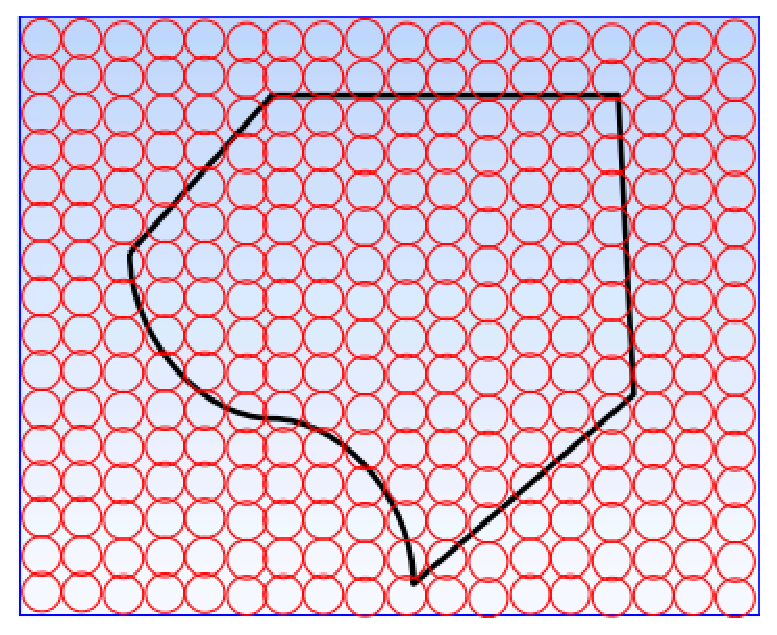
\includegraphics[width=0.95\textwidth,height=5cm]{figures/irregularity.eps}
  \caption{不规则图形面积计算}\label{fig:irr-mc}
  \end{minipage}
  \begin{minipage}[t]{0.3\linewidth}
  \centering
  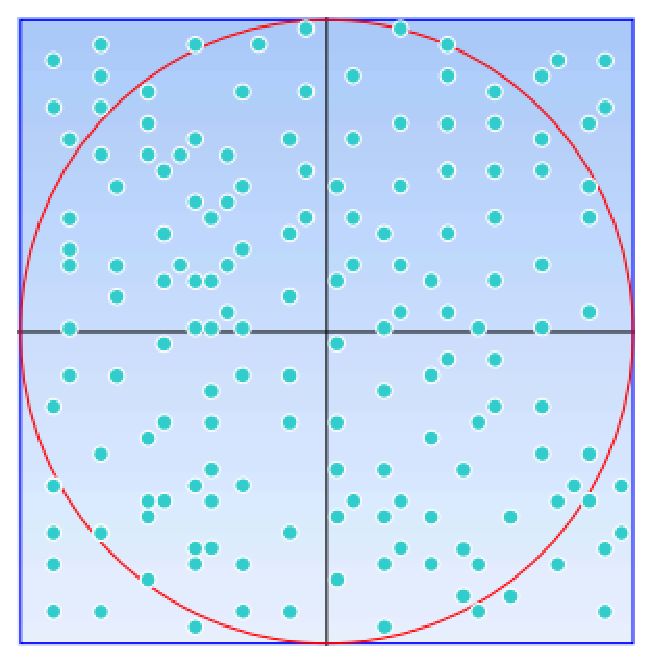
\includegraphics[width=0.95\textwidth,height=5cm]{figures/pi.eps}
  \caption{估计无理数$\pi$的值}\label{fig:pi-mc}
  \end{minipage}
  \begin{minipage}[t]{0.3\linewidth}
  \centering
  \includegraphics[width=0.95\textwidth,height=5cm]{figures/integration.eps}
  \caption{定积分计算}\label{fig:int-mc}
  \end{minipage}
\end{figure}

蒙特卡罗方法的模拟过程随机,也适合解决一些确定性问题。通常,蒙特卡罗方法包括两个基本步骤:1)利用计算机生成服从某种分布的随机样本,2)对样本做统计分析。当所求问题与某种随机事件出现的概率,或者某个随机变量的期望值存在对应关系时,我们通过“模拟实验”估计随机事件的概率,或随机变量的某些数字特征,并将其作为问题的解。由于蒙特卡罗方法需要生成大量的随机数,并且绝大多数分布都可以使用均匀分布$U(0,1)$构造,我们下面介绍几种生成服从均匀分布$U(0,1)$样本的方法。
\begin{proposition}[平方取中法]%(Middle Square Method, John von Neumann)
任取一个$m$位的整数$z_0$,依次使用$z_{i-1}^2$的中间$m$位构造序列$\{z_i\}_{i=1}^n$,则有\[x_i=z_i/10^m\sim U(0,1), i = 1, 2,\ldots,n.\]
\end{proposition}

\begin{proposition}[倍积取中法]
任取一个$m$位的整数$z_0$与$y$,依次使用$yz_{i-1}$的中间$m$位构造序列$z_i$,则有\[x_i=z_i/10^m\sim U(0,1), i = 1, 2,\ldots,n.\]
\end{proposition}

\begin{proposition}[一阶线性同余法]%(Linear Congruential Method)
指定$m=999563$、$y=47001$和初值$z_0=671800$,根据\[z_i=yz_{i-1} \pmod{m}\] 构造序列$\{z_i\}_{i=1}^n$,则有\[x_i=z_i/m\sim U(0,1), i = 1, 2,\ldots,n.\]
\end{proposition}

\begin{proposition}[一阶混合同余法]
指定$m=999563$、$w=1234$、$y=47001$ 和初值$z_0=671800$,根据\[z_i=w + yz_{i-1} \pmod{m}\] 构造序列$\{z_i\}_{i=1}^n$,则有\[x_i=z_i/m\sim U(0,1), i = 1, 2,\ldots,n.\]
\end{proposition}

\begin{proposition}[S阶混合同余法]
指定$m, w, y_1, y_2, \ldots, y_s$与$z_{-s+1}, z_{-s+2}, \ldots, z_0$,根据\[z_i=w + \sum\limits_{k=1}^s y_k z_{i-k} \pmod{m}\]构造序列$\{z_i\}_{i=1}^n$,则有\[x_i=z_i/m\sim U(0,1), i = 1, 2,\ldots,n.\]
\end{proposition}

随机数的生成方法具有重要用途,比如我们可以利用$U(0,1)$上的随机数间接地生成服从其他分布的随机数。

假设离散随机变量$X$的分布列是$P(X=x_i)=p_i, i=1,2,\ldots,n$,它的分布函数为
\begin{equation}
    F(x) = \left\{
    \begin{array}{rl}
    0, & x<x_1,\\
    p_1, & x_1\le x<x_2,\\
    p_1 + p_2, & x_2\le x<x_3,\\
    \cdots & \cdots\\
    \sum\limits_{i=1}^k p_i, & x_k \le x < x_{k+1}, \\
    \cdots & \cdots\\
    1, & x_n \le x.
    \end{array}
    \right.
\end{equation}
我们生成一个$U(0,1)$上的随机数$u$,如果$0\le u < F(x_1)$,则随机数为$x=x_1$。如果存在$F(x_{k-1})\le k < F(x_k)$,则随机数为$x=x_k$。

\begin{theorem}[反函数法]
假设随机变量$X\sim U(0,1)$,$F(z)$是一个连续分布函数且存在反函数,则随机变量$Z=F^{-1}(X)$的分布函数为$F(z)$。
\end{theorem}

\begin{property}
假设随机变量$X\sim U(0,1)$,对任意的$a,b\in \mathbb R$,只要$a<b$,则有
\[
    Z = a + (b-a)X\sim U(a,b).
\]
\end{property}
\begin{property}
假设随机变量$X\sim U(0,1)$,对任意的$\lambda,k>0$都有
\[
    Z=\big[-\frac{1}{\lambda}\ln(1-X)\big]^{1/k}
\]
服从参数为$\lambda,k$的\textbf{Weibull分布}$W(\lambda,k)$
\footnote{1927年,法国数学家Maurice Fr\'{e}chet\cite{frechet1927loi}最先给出此分布的定义。1933年Paul Rosin和Erich Rammler\cite{rossin1933laws}首次将其应用到碎末尺寸分布的研究。1951年,瑞典数学家和工程师Waloddi Weibull\cite{weibull1951statistical}对其进行详细解释。Weibull分布比\textbf{对数正态分布}具有更大的适用性,它是可靠性分析及轴承寿命检验的理论基础,被广泛应用于各种滚动轴承的寿命试验及高应力水平下的材料疲劳试验。},即
\begin{equation}
    f(x;\lambda,k) = \left\{
        \begin{array}{ll}
            \frac{k}{\lambda} (\frac{x}{\lambda})^{k-1} \exp\{-(\frac{x}{\lambda})^k\}, & x\ge 0,\\
            0,& x<0.
        \end{array}
    \right.
\end{equation}
当$k=1$时,$Z\sim \mathrm{Exp}(1/\lambda)$。
\end{property}

\begin{theorem}[Box-Muller方法]
假设$X_1\sim U(0,1), X_2\sim U(0,1)$,且$X_1,X_2$相互独立,则变量
\[
    Z_1=(-2\ln X_1)^{1/2} \cos (2\pi X_2)
\]
和变量
\[
    Z_2=(-2\ln X_1)^{1/2} \sin (2\pi X_2)
\]
相互独立,并且都服从标准正态分布$N(0,1)$。
\end{theorem}

\begin{theorem}
假设$X_1,X_2,\ldots,X_n$是$n$个独立同分布于$U(0,1)$的随机变量,则有$E(X_i)=1/2$,$\var(X_i)=1/12$。由Linderberg-Levy中心极限定理知,当$n\rightarrow \infty$时,
\begin{equation}
    Y = \frac{\sum\limits_i X_i - n/2}{\sqrt{n/12}} \sim N(0,1).
\end{equation}
当$n=12$时,$Y=\sum\limits_i X_i - 6$近似服从$N(0,1)$。
\end{theorem}
利用Box-Muller方法或者中心极限定理,我们可以在均匀分布的基础上构造出标准正态分布,进而构造出一般正态分布、三大抽样分布等,从而可以生成相应分布下的随机数。为了能够处理特别高维的概率分布随机抽样,提高随机抽样的效率问题,人们开始研究高级的随机模拟技术。

\subsection{马尔科夫链蒙特卡罗法}
1953年,Nicholas Metropolis等人\cite{metropolis1953equation} 提出一种新的随机模拟方法\textbf{马尔科夫蒙特卡罗法}(Markov Chain Monte Carlo,MCMC)(也称\textbf{动态蒙特卡罗方法}),70年代Keith Hastings\cite{hastings1970monte}将其扩展为更一般的形式,称为\textbf{Metropolis-Hastings算法}。Metropolis-Hastings 算法是MCMC的基础方法,并陆续演化出许多新的抽样方法,比如目前在MCMC 方法中最常用的\textbf{Gibbs抽样}。2009年,斯坦福大学统计学教授Persi Diaconis\cite{diaconis2009markov}使用MCMC 方法成功破解犯人密码。

1984年,Stuart Geman和Donald Geman\cite{geman1984stochastic}两兄弟提出一种新的抽样方法:Gibbs抽样,它是Metropolis-Hastings算法的一个特例($\alpha=1$),用于抽取服从多元分布的样本。

\section{参数估计}
人口普查中心要确定全国人口的身高分布,它不可能去统计全国所有人口的身高,只能做出一个模型假设,利用一定的采样数据评估模型的参数。比如,假设人口身高服从正态分布,人口普查中心只要从不同地区采样统计一部分人口的身高数据,然后通过各种统计方法估计人口正态分布的均值和方差两个参数。一般地,参数估计的形式有两种:\textbf{点估计}与\textbf{区间估计}。前者给出一个具体的数值,后者是给出未知参数的一个区间,可以反映参数估计结果的精度。我们首先介绍三种常用的点估计方法:\textbf{最大似然估计}(Maximum Likelihood Estimate,MLE)、\textbf{贝叶斯估计}(Bayesian Estimate)和\textbf{最大后验估计}(Maximum a Posteriori Estimate,MAP),再介绍区间估计的内容。

\subsection{最大似然估计}
最大似然估计最早由高斯提出,1912年Fisher再次提出,并证明了此方法的一些性质。它提供了一种给定观测数据评估模型参数的方法,即在模型确定的条件下,估计模型的参数。最大似然估计假设所有观测数据$X=\{x_1,\ldots,x_n\}$独立同分布于含参总体分布$p(x; \theta)$,并称它们的联合概率
\[
    p(X;\theta) = p(x_1,x_2,\ldots, x_n; \theta) = \prod\limits_i p(x_i; \theta)
\]
为\textbf{似然函数}。最大似然估计对参数$\theta$不作任何假设,直接从参数空间搜索一个可以使似然函数最大化的最优值,记作$\hat \theta_\mathrm{MLE}$:
\begin{equation}
   \hat \theta_\mathrm{MLE} = \argmax\limits_\theta p(X;\theta) = \argmax\limits_\theta \prod\limits_i p(x_i; \theta).
\end{equation}
由于连乘形式的似然函数不容易直接优化,通常对其应用对数变换转换为加和形式。根据对数函数的单调性可知,最大化似然函数等价于最大化对数似然函数,则有:
\begin{equation}
   \hat \theta_\mathrm{MLE} = \argmax\limits_\theta \log p(X;\theta) = \argmax\limits_\theta \sum\limits_i \log p(x_i; \theta).
\end{equation}

\begin{example}[序例\ref{eg:pistat}]
\begin{figure}[htbp]
  \centering
  \includegraphics[width=0.85\textwidth, height=6cm]{figures/pisumdist.eps}\\
  \caption{圆周率$\pi$值前1,000万位小数连续数字串加和分布图}\label{fig:pisumdist}
\end{figure}
在观察圆周率$\pi$的单个数字的分布状况以后,我们进而考察连续数字串的特征。对小数点后的连续的数字串加和,分析不同长度数字串数字加和的分布,如图
\ref{fig:pisumdist} 所示,数字串长度从左至右分别是30、40和50,呈现出明显的正态分布特征,横轴是数字串的和,纵轴对应加和出现的频次。如果记数字串加和、频次统计数据为$\{(x_i,n_i),i\in \mathbb N\}$,我们利用这些统计数据,确定正态分布参数的最大似然估计。
假设$X\in N(\mu,\sigma)$,使用固定长度的数字串观测数据建立对数似然函数
\[
\begin{array}{lcl}
    L(x_1,x_2,\ldots; \mu,\sigma) &=& \log \prod\limits_i \big[\frac{1}{\sqrt{2\pi} \sigma} \exp\big\{-\frac{(x_i-\mu)^2}{2\sigma^2}\big\} \big]^{n_i}\\
    & = & \sum\limits_i n_i \big[\log \frac{1}{\sqrt{2\pi} \sigma} - \frac{(x_i-\mu)^2}{2\sigma^2}\big]\\
    & = & (-\log \sqrt{2\pi} - \log\sigma) \sum\limits_i n_i - \frac{1}{2\sigma^2} \sum\limits_i n_i (x_i-\mu)^2,
\end{array}
\]
从而可以确定参数$\mu$和$\sigma$的最大似然估计$\hat \mu_\mathrm{MLE}$和$\hat \sigma_\mathrm{MLE}$,则有
\[
    \hat \mu_\mathrm{MLE} = \sum\limits_i \omega_i x_i,~~~\hat \sigma_\mathrm{MLE} = \sqrt{\sum\limits_i \omega_i (x_i-\hat \mu_\mathrm{MLE})^2},~~~\omega_i = \frac{n_i}{\sum\limits_i n_i},~~~\sum\limits_i \omega_i = 1,
\]
所以$\hat \mu_\mathrm{MLE}^{30}=136$,$\hat \sigma_\mathrm{MLE}^{30}=15.72$;$\hat \mu_\mathrm{MLE}^{40}=181$,$\hat \sigma_\mathrm{MLE}^{40}=18.14$;$\hat \mu_\mathrm{MLE}^{50}=226$,$\hat \sigma_\mathrm{MLE}^{50}=20.27$。
\end{example}

\subsection{贝叶斯估计}
在统计学中有两大学派:频率学派(Frequentists,也称经典学派)与贝叶斯学派(Bayesians)。频率学派认为,统计推断是根据样本信息对总体分布或总体特征进行推断,主要使用两种信息:\textbf{总体信息}和\textbf{样本信息}。贝叶斯学派认为,在总体信息与样本信息之外,统计推断还应该使用第三种信息:\textbf{先验信息}(Prior Information)。贝叶斯统计学与经典统计学的差别就在于是否利用先验信息。贝叶斯学派的一个基本观点是:任意一个未知参数都可看作是随机变量,可以使用一个概率分布描述它,这种分布称作\textbf{先验分布}(Prior Distribution)。在获得样本信息之后,总体分布、样本与先验分布通过贝叶斯公式结合起来,构造出关于未知参数的\textbf{后验分布}(Posteriori Distribution),并在后验分布的基础之上开展统计推断。现在经典学派也已经接受这种观点\cite{Lehmann2001Theory},两派的争论焦点聚集在如何利用先验信息合理地确定先验分布。

贝叶斯学派则将未知参数$\theta$看作随机变量,而总体依赖于参数的概率函数记作$p(x|\theta)$,它表示给定随机变量$\theta$的某个取值,总体的条件概率函数。基于这种思想,样本$X=\{x_1,\ldots,x_n\}$的产生实际上经历两个基本步骤:根据模型参数的先验分布$p(\theta)$产生样本$\theta$,再从条件概率分布$p(X|\theta)$ 中产生一组样本。由此,样本$X$的联合条件概率函数表示如下:
\begin{equation}
    p(X|\theta) = p(x_1,x_2,\ldots,x_n|\theta) = \prod\limits_i p(x_i|\theta),
\end{equation}
根据贝叶斯定理,给定参数的先验分布、样本的联合条件概率分布,我们可以确定后验分布:
\begin{equation}
    p(\theta|X) = \frac{p(X|\theta)p(\theta)}{p(X)} = \frac{p(X|\theta)p(\theta)}{\int_\Theta p(X|\theta) p(\theta) d\theta}.
\end{equation}
后验分布用总体和样本信息对先验分布进行调整,集中总体、样本与先验知识中所有关于参数$\theta$的信息,它比$p(\theta)$更接近于$\theta$的实际情况。
在后验分布$p(\theta|X)$的基础上估计$\theta$,目前存在两种最常用的方法:\textbf{后验期望估计}(Posteriori Mean Estimate,PME)和\textbf{最大后验估计}
(Maximum a Posteriori Estimate,MAP),统称\textbf{贝叶斯估计}。
\begin{enumerate}
  \item \textbf{后验期望估计}:使用后验分布的均值作为$\theta$的点估计,记作$\hat \theta_\mathrm{PME}$,则有
        \begin{equation}
            \hat \theta_\mathrm{PME} = E(\theta|X) = \int_\Theta \theta p(\theta|X) d\theta.
        \end{equation}
  \item \textbf{最大后验估计}:使用后验分布的密度函数最大值点作为$\theta$的点估计,记作$\hat\theta_\mathrm{MAP}$,则有
          \begin{equation}
            \max\limits_\theta p(\theta|X) = \max\limits_\theta \frac{p(X|\theta) p(\theta)}{p(X)},
          \end{equation}
        由于$p(X)$不依赖于随机变量$\theta$,忽略分母部分可得:
        \begin{equation}
            \hat\theta_\mathrm{MAP} = \argmax\limits_\theta p(\theta) \prod\limits_i p(x_i|\theta)
            = \argmax\limits_\theta \Big[\sum\limits_i \log p(x_i|\theta) + \log p(\theta)\Big].
        \end{equation}
        对比最大似然估计和最大后验估计可以发现,最大后验估计实际上是最大似然估计的规则化模型,而其规则化项正是引入的先验概率的对数。
\end{enumerate}
贝叶斯估计与最大似然估计都是通过观测数据估计模型参数,但贝叶斯估计同时利用了未知参数的先验知识。如果先验分布可以准确描述待估参数,则贝叶斯估计比最大似然估计更加准确。此外,最大似然估计中的$p(x;\theta)$和最大后验估计及贝叶斯估计中的$p(x|\theta)$形不同而义同。最大似然估计的思想源于古典学派,将未知参数$\theta$ 看作一个普通变量,则总体依赖于参数$\theta$的概率函数记作$p(x;\theta)$,表示参数空间$\Theta$中不同的$\theta$对应不同的分布。最大后验估计和贝叶斯估计则反映贝叶斯学派的思想,将未知参数$\theta$看作随机变量,而总体依赖于参数的概率函数记作$p(x|\theta)$,它表示给定随机变量$\theta$ 的某个取值,总体的条件概率函数。

从贝叶斯公式可以看出,确定先验分布是展开贝叶斯统计推断的一个基本前提。关于先验分布的确定方法很多,目前最常用的一类先验分布是\textbf{共轭先验分布}。选择共轭先验分布从数学上可以为贝叶斯统计推断提供极大的便利,这也正是\textbf{隐含狄利克雷分布}(Latent Dirichlet Allocation, LDA)的理论基础。
\begin{definition}[共轭先验分布]
假设$\theta$是总体参数,如果对任意的样本观测值$X=\{x_1,\ldots,x_n\}$,参数$\theta$的\textbf{后验分布}$p(\theta|X)$与\textbf{先验分布}$p(\theta)$属于同一个分布族(Family),则称后验分布$p(\theta|X)$与先验分布$p(\theta)$是\textbf{共轭分布}(Conjugate Distribution),先验分布$p(\theta)$是关于似然函数$p(X|\theta)$的一个\textbf{共轭先验}(Conjugate Prior)。
\end{definition}

\begin{example}
假设事件$A$在一次试验中发生的概率是$\theta$,我们对试验进行$n$次独立观测$X=\{x_1,x_2,\ldots,x_n\}$,$x_i$表示第$i$次试验事件$A$是否发生,即
\[
    x_i = \left\{
    \begin{array}{rl}
        1, & \text{事件$A$发生},\\
        0, & \text{事件$A$未发生}.
    \end{array}
    \right.
\]
对于任意的$i\in\{1,2,\ldots,n\}$,$x_i$独立且都服从两点分布。请根据观测数据确定参数$\theta$的最大似然估计$\hat \theta_\mathrm{MLE}$、最大后验估计$\hat\theta_\mathrm{MAP}$ 与后验期望估计$\hat \theta_\mathrm{PME}$。
\end{example}
\begin{solu}
由于$p(x;\theta)=\theta^x (1-\theta)^{1-x}$,构造对数似然函数
\[
    L(x_1,x_2,\ldots,x_n;\theta) = \log\prod\limits_i p(x_i;\theta) = \sum\limits_i \big[x_i \log \theta + (1-x_i)\log(1-\theta)\big],
\]
对它求关于$\theta$的导数,可以解出参数$\theta$的最大似然估计
\begin{equation}
    \hat\theta_\mathrm{MLE} = \argmax\limits_{\theta\in (0,1)}L(x_1,x_2,\ldots,x_n;\theta) = \frac{1}{n} \sum\limits_i x_i \triangleq \frac{z}{n}.
\end{equation}
其中$z=\sum\limits_i x_i$表示$n$次试验事件$A$发生的次数。根据贝叶斯建议的“等同无知”原则假定参数$\theta$的先验分布为均匀分布$U(0,1)=\mathrm{Beta}(1,1)$,则有
\[
    p(\theta) = \frac{1}{1-0} = 1, 0<\theta<1,
\]
可以确定参数$\theta$与观测数据的联合分布为
\[
    p(X,\theta) = p(X|\theta) p(\theta) = \prod\limits_i p(x_i|\theta) = \prod\limits_i [\theta^{x_i} (1-\theta)^{1-x_i}] = \theta^z (1-\theta)^{n -z}.
\]
现在我们可以直接确定最大后验估计
\begin{equation}
    \hat\theta_\mathrm{MAP} = \argmax\limits_{\theta\in (0,1)} p(X,\theta) = \hat\theta_\mathrm{MLE} = \frac{z}{n}.
\end{equation}
根据贝叶斯定理,给定观测数据$X=\{x_1,x_2,\ldots,x_n\}$的条件下,我们可以确定参数$\theta$的后验概率
\[
    p(\theta|X) = \frac{p(X,\theta)}{\int_0^1 p(X,\theta) d\theta}, 1<\theta < 1.
\]
我们知道
\[
    \int_0^1 \theta^z (1-\theta)^{n-z} d\theta = \frac{\Gamma(z+1)\Gamma(n-z+1)}{\Gamma(z+2)},
\]
从而可得后验概率
\[
    p(\theta|X) = \frac{\Gamma(z+1)\Gamma(n-z+1)}{\Gamma(z+2)} \theta^z (1-\theta)^{n -z}, 1<\theta < 1.
\]
结果表明$\theta|X\sim \mathrm{Beta}(z+1,n-z+1)$,参数$\theta$的后验期望估计为
\begin{equation}
    \hat\theta_\mathrm{PME} = E(\theta|X) = \frac{z+1}{n+2}.
\end{equation}
\end{solu}

\subsection{区间估计}
区间估计的目标是确定两个统计量
\[
    \hat \theta_L=\hat\theta_L(x_1,\ldots,x_n) < \hat \theta_U=\hat\theta_U(x_1,\ldots,x_n),
\]
利用样本观测值,使$\theta$以概率$P(\hat\theta_L \le \theta \le \hat\theta_U)$落入区间$[\hat\theta_L,\hat\theta_U]$内。自然地,区间长度$\hat\theta_U-\hat\theta_L$越大,参数$\theta$落入区间$[\hat\theta_L,\hat\theta_U]$的可能性就越高。最理想的情景是\textbf{高概率短区间}:参数$\theta$以很高的概率落入一个狭窄的区间$[\hat\theta_L,\hat\theta_U]$。为此,我们限定参数$\theta$ 落入区间$[\hat\theta_L,\hat\theta_U]$内的概率上界,并引出\textbf{置信区间}(Confidence Interval)的概念。

\begin{definition}
假设$\theta\in \Theta$是总体的一个参数,$x_1,x_2,\ldots,x_n$是取自总体的$n$个样本,给定一个$0<\alpha<1$,如果存在两个统计量$\hat \theta_L=\hat\theta_L(x_1,\ldots,x_n)$和$\hat \theta_U=\hat\theta_U(x_1,\ldots,x_n)$,对任意的$\theta\in \Theta$,都有
\begin{equation}
    P_\theta(\hat\theta_L \le \theta \le \hat\theta_U) \ge 1-\alpha,
\end{equation}
则称随机区间$[\hat\theta_L,\hat\theta_U]$是$\theta$的\textbf{置信水平}(Confidence Level)为$1-\alpha$的\textbf{置信区间},$\hat\theta_L$和$\hat\theta_U$分别称作$\theta$的\textbf{置信下限}和\textbf{置信上限}。如果对任意的$\theta\in \Theta$,都有
\begin{equation}
    P_\theta(\hat\theta_L \le \theta \le \hat\theta_U) = 1-\alpha,
\end{equation}
则称$[\hat\theta_L,\hat\theta_U]$是$\theta$的$1-\alpha$\textbf{同等置信区间}。
\end{definition}

\section{假设检验}
\textbf{参数估计}(Parameter Estimation)和\textbf{假设检验}(Hypothesis Testing)是统计推断的主要内容,本节开始介绍假设检验的内容。我们从下面四个例子引出假设检验问题。
\begin{example}\label{eg:packingmachine}
某药品生产车间用粉剂定量自动包装机包装粉剂药品,每袋标准重量为50 mg。长期实践表明该设备包装的这一药品重量服从正态分布,且标准差为1.5 mg。现从某天的包装产品中随机抽取9袋,精确秤得它们的重量分别为
\[49.5, 50.6, 51.8, 52.1, 49.3, 51.1, 52.0, 51.5, 50.0\]
它们的平均值为50.9 mg,那么当日该包装机是否正常工作?
\end{example}
\begin{example}\label{eg:metalprod}
某工厂生产的合金强度服从正态分布$N(\theta,16)$,其中$\theta$的设计值不低于110 Pa。为保证质量,该厂每天对生产情况做例行检查,以判断生产是否正常进行。某天从生产中随机抽取25块合金,测得强度值为$x_1,\ldots,x_25$,其均值为$\bar x=108$ Pa,问当日生产是否正常?
\end{example}
\begin{example}\label{eg:alterpara}
假设总体$X\sim N(\theta,\sigma^2)$,$\sigma^2$已知,而$\theta$只能取两个值$\theta_0$或者$\theta_1$并且$\theta_0<\theta_1$,现从总体$X$中抽取的容量为$n$的样本$x_1,x_2,\ldots,x_n$,那么总体的均值是$\theta_0$还是$\theta_1$?
\end{example}
\begin{example}\label{eg:pollutedmilk}
将0.1 ml受细菌污染的牛奶均匀涂在1 cm$^2$的切片上,用显微镜观察切片每个小网格内的细菌菌落数目。根据400(20$\times$20)个小网格的计数结果,统计出如表
\ref{tbl:pollutedmilk}所示。试问菌落数是否服从泊松分布?
\begin{table}[htbp]
    \caption{污染牛奶切片菌落统计表}
    \centering
    \begin{tabular}{|l|l|l|l|l|l|l|l|l|l|l|l|l|l|l|l|l|l|l|l|l|}
      \hline
       菌落数 & 0 & 1 & 2 & 3 & 4 & 5 & 6 & 7 & 8 & 9 & 10 & 19\\
      \hline
       频~~~~数 & 56 & 104 & 80 & 62 & 42 & 27 & 9 & 9 & 5 & 3 & 2 & 1\\
      \hline
    \end{tabular}
    \label{tbl:pollutedmilk}
\end{table}
\end{example}


假设检验是一种根据简单随机抽样抽取的样本信息来判别总体是否具有某种性质的统计推断方法。两个例子代表两类假设检验问题,分别属于参数和非参数假设检验问题。\textbf{参数假设检验}在已知总体分布函数类型的前提下,对分布函数的未知参数提出某种假设,然后利用样本信息对所提假设进行检验,根据检验结果作出\textbf{接受}或者\textbf{拒绝}所提假设的判断。\textbf{非参数假设检验}是在总体分布函数类型未知的条件下,根据样本信息对分布类型的假设进行检验,从而对总体分布类型作出判断。本节重点在参数假设检验(例\ref{eg:packingmachine}、\ref{eg:metalprod}和\ref{eg:alterpara}),下一节通过例\ref{eg:pollutedmilk}具体介绍非参数假设检验。

\subsection{参数假设检验}
一般地,假设检验包含五个主要步骤:建立假设、选择检验统计量并给出拒绝域形式、选择显著性水平、给出拒绝域、作出判断。

\begin{enumerate}[Step 1.]
  \item
  \textbf{建立假设}:假设检验需要把一个被检验的假设称作\textbf{原假设}(Null Hypothesis),记作$H_0$。通常,原假设无法轻易否定。当$H_0$被拒绝时而接受的假设称作\textbf{备择假设}(Alternative Hypothesis),记作$H_1$。两个假设$H_0$和$H_1$成对出现。在例\ref{eg:packingmachine}中,包装机包装药品的重量服从正态分布$N(\theta,\sigma^2)$,我们已知参数$\sigma=1.5$,对于判断机器包装重量的均值是否等于$\theta_0=50$ mg,可以建立如下两个假设:\[H_0: \theta\in \Theta_0 =\{\theta: \theta = \theta_0\} ~~~~~~ \textrm{vs}  ~~~~~~ H_1: \theta\in \Theta_1 =\{\theta: \theta \ne \theta_0\}.\]
  这种形式的参数假设检验称作\textbf{双侧检验}(Two-sided Testing),还有一种形式的假设检验称作\textbf{单侧检验}(One-sided Testing):
  \[H_0: \theta\in \Theta_0 =\{\theta: \theta \ge \theta_0\} ~~~~~~ \textrm{vs}  ~~~~~~ H_1: \theta\in \Theta_1 =\{\theta: \theta < \theta_0\},\] 或者\[H_0: \theta\in \Theta_0 =\{\theta: \theta \le \theta_0\} ~~~~~~ \textrm{vs}  ~~~~~~ H_1: \theta\in \Theta_1 =\{\theta: \theta > \theta_0\}.\]
  \item
  \textbf{选择检验统计量,给出拒绝域形式}:根据样本数据对原假设进行判断总是通过一个统计量来完成,这个统计量称作\textbf{检验统计量}。通常,检验统计量$T(x_1,x_2,\ldots,x_n)$也是一个\textbf{充分统计量}。在确定检验统计量以后,从而可以建立原假设被拒绝的\textbf{拒绝域}(Rejection Region),它是样本空间的一个子集,记作$W$。一般地,拒绝域的形式依赖于参数假设检验的形式,如果是单侧检验,则拒绝域是一个连续的样本空间子集:
  \[W=\{(x_1,x_2,\ldots,x_n): T(x_1,x_2,\ldots,x_n; \theta) \le \tau\}\]或者\[W=\{(x_1,x_2,\ldots,x_n): T(x_1,x_2,\ldots,x_n; \theta) \ge \tau\}.\]
  如果是双侧检验,则拒绝域由两个不相交的连续样本空间子集构成:
  \[W=\{(x_1,x_2,\ldots,x_n): |T(x_1,x_2,\ldots,x_n; \theta)| \ge \tau\}.\]
  当拒绝域确定后,检验的判断准则也相应地确定。如果$(x_1,x_2,\ldots,x_n)\in W$,则认为$H_0$不成立,拒绝原假设;如果$(x_1,x_2,\ldots,x_n)\in A$,则认为$H_0$成立,接受原假设,$A$称作\textbf{接受域}(Acceptance Region)。
  例\ref{eg:packingmachine}所示的假设检验属于双侧检验,由于$\bar x\sim N(\mu, \sigma^2/n)$,我们选择统计量
  \[T(x_1,x_2,\ldots,x_n; \theta)=\frac{\bar x - \mu_0}{\sigma/\sqrt{n}},\]并构造双侧拒绝域。
  \item
  \textbf{选择显著性水平}:由于抽样的随机性和小概率事件的发生,假设检验可能犯下两类错误。第一类错误(Type I Error)是$H_0$为真,但是样本观测值落在拒绝域内,从而拒绝原假设$H_0$,其发生的概率称作\textbf{拒真概率},记作$\alpha$,即
  \[\alpha = P(\text{拒绝}H_0|H_0\text{为真}).\]%=P((x_1,x_2,\ldots,x_n)\in W)
  第二类错误(Type II Error)是$H_1$为真,但是样本观测值落在接受域内,从而接受原假设$H_0$,其发生的概率称作\textbf{纳伪概率},记作$\beta$,即
  \[\beta = P(\text{接受}H_0|H_1\text{为真}).\]%=P((x_1,x_2,\ldots,x_n)\in \overline W)
  一般地,拒真概率越小,则纳伪概率越大;反之,拒真概率越大,纳伪就概率越小。为了平衡两种错误,统计学家Jerzy Neyman与Egon Pearson提出显著性检验优先的基本原则:在控制出现第一类错误$\alpha$的条件下,寻求使出现第二类错误$\beta$尽可能小的检验。$\alpha$也称\textbf{显著性水平}(Significance Level),通常取值$\{0.01,0.05,0.10\}$,$1-\alpha$称作\textbf{置信水平}(Confidence Level),$1-\beta$称作\textbf{检验效能}(Power of Testing)。
  \item \textbf{给出拒绝域}:
  在确定显著性水平后,我们可以确定出检验的拒绝域$W$。对于例\ref{eg:packingmachine},如果取$\alpha=0.05$,则拒绝域
  \[
    W=\{(x_1,x_2,\ldots,x_n): |\frac{\bar x-\theta_0}{\sigma\sqrt n}| \ge \Phi^{-1}(\alpha/2)\} = \{(x_1,x_2,\ldots,x_n): |\frac{\bar x-\theta_0}{\sigma/\sqrt n}| \ge 1.96\}.
  \]
  \item \textbf{作出判断}:
  由于$\bar x=50.9$,则\[
    \frac{\bar x - \theta_0}{\sigma/\sqrt n}=\frac{50.9-50}{1.5/3}=1.8 < 1.96
  \]
  接受原假设$H_0$。
\end{enumerate}

\subsection{非参数假设检验}%Nonparametric Hypothesis Test
\begin{definition}[经验分布函数]
设$X_1, X_2, \ldots, X_n$是来自总体$X$的样本,$x_1, x_2, \ldots, x_n$是对应观察值,将它们按照观察值的大小递增顺序排列生成$x_{(1)}\le x_{(2)}\le \cdots \le x_{(n)}$,构造函数:
\[
    F_n(x) = \left\{
    \begin{array}{rl}
    0, & x<x_{(1)},\\
    \dfrac{k}{n}, & x_{(k)}\le x<x_{(k+1)}, k = 2,3,\ldots, n-1,\\
    1, & x \ge x_{(n)}.
    \end{array}
    \right.
\]
则称$F_n(x)$是总体$X$的\textbf{经验分布函数}(Empirical Distribution Function)。对应地,总体$X$的分布函数$F(x)$称作\textbf{理论分布函数}(Theoretical Distribution Function)。
\end{definition}

在20世纪30年代,前苏联统计学家Valery Ivanovich Glivenko与意大利数学家Francesco Paolo Cantelli证明了一个极限定理,并成为统计学基础理论一个重要的结论。
\begin{theorem}[Glivenko-Cantelli定理]
设$x_1,x_2,\ldots, x_n$是取自总体分布函数为$F(x)$的样本,$F_n(x)$是其经验分布函数,当$n\rightarrow +\infty$时,有
\[
    P\{\sup\limits_{-\infty<x<+\infty} |F_n(x) - F(x)| \rightarrow 0\} = 1.
\]
\end{theorem}
Glivenko-Cantelli定理表明,当$n$充分大时,经验分布函数是总体分布函数$F(x)$的一个良好的近似。经典统计学中一切统计推断都以样本为依据,其理由就在于此。
我们可以利用Glivenko-Cantelli定理进行非参数假设检验:设总体$X$的分布函数为$F(x)$,对一个给定的分布$F_0(x)$,考虑原假设$H_0: F(x) = F_0(x)$,
根据Glivenko-Cantelli定理:当样本容量$n$充分大时,样本的经验分布函数$F_n(x)$是总体$X$分布函数$F(x)$的一个很好的近似。当原假设$H_0$为真时,$F_n(x)$与$F_0(x)$之间的差应该是一个小量。

\begin{theorem}
设总体$X$的分布函数$F(x)$连续,$X_1,X_2,\ldots, X_n$是来自总体$X$的样本,则对任意的分布函数$F_0(x)$,如果$H_0:F(x)=F_0(x)$成立,必然有
\begin{equation}
    \lim\limits_{n\rightarrow +\infty} P(D^{(n)} < \frac{\lambda}{\sqrt n}) = K(\lambda),
\end{equation}
其中,$D^{(n)}$称作\textbf{Kolmogorov统计量}
\begin{equation}
    D^{(n)} = \sup\limits_{-\infty<x<+\infty} |F_n(x) - F_0(x)| = \max\limits_{1\le i\le n} \big\{|\frac{i}{n} - F_0(x_{(i)}|,|\frac{i-1}{n} - F_0(x_{(i)}|\big\}
\end{equation}
是经验分布函数$F_n(x)$与$F_0(x)$的最大间隔,满足\textbf{分布无关性}。$K(\lambda)$是Kolmogorov分布密度函数
\begin{equation}
    K(\lambda) =\left\{
    \begin{array}{rl}
    \sum\limits_{k=-\infty}^{+\infty} (-1)^k e^{-2k^2\lambda^2}, & \lambda > 0,\\
    0, & \lambda \le 0.
    \end{array}
    \right.
\end{equation}
\end{theorem}

\begin{definition}[Kolmogorov–Simrnov检验]
设总体$X$的分布函数$F(x)$连续,$X_1,X_2,\ldots, X_n$是来自总体$X$的样本,则对任意的分布函数$F_0(x)$,考虑原假设$H_0:F(x)=F_0(x)$,在显著性水平$\alpha$下的拒绝域形式为:
\[
    W = \{(x_1,x_2,\ldots, x_n): D^{(n)} \ge D_{1-\alpha}^{(n)}\}.
\]
其中$P(D^{(n)} \ge D_{1-\alpha}^{(n)}) = \alpha$,并且$D_{0.99}^{(n)} \approx 1.63/\sqrt n$,$D_{0.95}^{(n)} \approx 1.36/\sqrt n$,$D_{0.9}^{(n)} \approx 1.23/\sqrt n$。
\end{definition}

\subsection{显著性检验}
为了衡量模型之间是否存在显著性的差异,有两种办法:其一,直接比较数值差异,其二是确定这种差异是否具有统计显著性(Statistical Significance)。通常,数值差异并不意味着具有统计显著性差异,比如\cite{gomes2013learning}通过在多个数据集上分析基准排序学习算法发现,排序学习模型尽管相比最佳特征具有显著的数值差异,经过统计分析,这种差异不具有统计学意义。

假设存在两个系统A和B,在每个系统上都执行$n$次试验,相应的分别得到两组试验结果$X = (x_1,\ldots, x_n), Y = (y_1,\ldots, y_n)$。 由此,可以计算系统A 和B 实验结果的偏差$Z = X - Y$。$Z$包含了$n$ 次试验偏差,相应的可以利用均值($\mu$)、方差($\sigma$)、给定的置信度(如95\%),通过查询$t$分布分位数表,就可以构建偏差的置信区间(Confidence Interval)$\mu \pm t \sqrt{\sigma/n}$。如果置信区间含有0,则表明两个系统试验结果是没有显著性差异的\cite{jain1991art}。

统计显著性从统计意义上保证了系统之间实验结果的差异性是真实可信的,而非仅仅出于偶然。比如,某种疾病的治疗方案有两种:A 和B,如果通过A、B治疗方案的病人都是100位,痊愈的比例分别是100\%、50\%,显然A 方案相比B治疗效果更为显著。假设接受A方案的病人只有1个,而接受B方案的有两个,同样的治愈率(100\% 与50\%)所反映的显著性就大打折扣。再设想,如果通过相同的治疗分组,治愈率分别是66\%,60\%,那么二者的差异性就不是那么明显了
\footnote{Cancer Guide:\href{http://cancerguide.org/significance.html}{http://cancerguide.org/significance.html}}。

统计显著性具有两个基本的特点:(1)如果数值差异越大,则出于偶然性的可能性越低;(2)根据大数定理,实验的样本越大,则观察到的差异性越能够反映真实的差异。

统计检验首先假设比对组实验结果是相同的,然而从数学上估计比对组之间差异出于偶然的概率,我们称之为p 值(p-Value),p值越大,则差异显著性就越弱,反之,比如$p<0.05$,则表明差异是显著的。

给定两组样本$x = (x_1,\ldots,x_n), y = (y_1,\ldots, y_n)$,为了比较二者之间的差异,一般会选择比较两组样本的样本均值,实际上样本均值的差异并不能反映整体差异。

显著性差异是一种有量度的或然性评价。比如说$x,y$两组样本在$p=0.05$水平上具有显著性差异,也即是说两组样本具有显著性差异的可能性是95\%,另外5\%的可能性是没有差异。这5\%的差异是由随机误差造成的。

\textbf{显著性检验}(Significance Test),又称\textbf{假设检验}(Hypothesis Test),有多种检验方法,如$t$检验、$F$检验和$\chi$检验等。

$t$检验基本步骤:
\begin{enumerate}
  \item 计算样本差异
  \[
    z = (z_1,\ldots,z_n)
  \]
  其中,$z_i = y_i - x_i,i=1,\ldots,n$。
  \item 计算样本平均差异
  \[
    \bar{z} = \sum\limits_i z_i
  \]
  \item 计算样本标准差
  \[
    s_z = \sqrt{\frac{1}{n-1}\sum\limits_i (z_i - \bar{z})^2}
  \]
  \item 计算统计量$t$
  \[
    t = \frac{\bar{z}}{s_z/\sqrt{n}}
  \]
  \item 根据样本大小$n$和$p$值(通常取$p=0.05,p=0.01$),查$t$分布表:$t_p(n-1)$
  \item 如果$|t|>t_p(n-1)$,则可以断定差异显著。
\end{enumerate}

\section{Wilcoxon-Mann-Whitney检验}
Wilcoxon-Mann-Whitney检验~\cite{wilcoxon1945individual,mann1947test},是一种无参检验方法,也称Mann-Whitney U检验、Wilcoxon秩和检验(Rank Sum Test),用于检验(推断)两组随机样本(分布)之间的差异性。WMW 检验的零假设(Null Hypothesis)是两组样本取自于性质相同的分布,它不是计算平均值的差异性,而是根据两组样本名次之和,计算出U-统计量以作检验。

给定随机变量$X$的样本数据$\{x_i\}_{i=1}^m$,随机变量$Y$的样本数据$\{y_j\}_{j=1}^n$,则U-统计量定义为:
\begin{equation}
    U = \frac{1}{mn} \sum\limits_{i=1}^m \sum\limits_{j=1}^n I(x_i > y_j)
\end{equation}
U-统计量实际上是对同序概率(Concordance Probability)$P(X>Y)$的一个估计量,如果以$X$,$Y$为坐标轴绘制ROC曲线,AUC与U-统计量等价
\cite{hanely1982meaning}。

在二元分类问题中,假设$x_1,\ldots,x_m$是分类器对正例的预测结果,$y_1,\ldots,y_n$是对负例的预测结果。将所有预测结果升序排列,我们可以根据所有正例的排名计算统计量$U$:
\begin{equation}
    U = \frac{1}{mn} \big[\sum\limits_{i=1}^m r_i - \frac{1}{2} m(m-1) \big]
\end{equation}
其中,$r_i$表示预测结果$x_i$的排名。在最理想的条件下,所有正例都应该得到大于负例的预测结果,从而有
\begin{equation}
    U = \frac{1}{mn}\big[(n+1) + (n+2) + \ldots + (n+m) - \frac{1}{2} m(m-1)\big] = 1,
\end{equation}
最不济的分类器完全预测错误,对应地有
\begin{equation}
    U = \frac{1}{mn}\big[(1 + 2 + \ldots + m)  - \frac{1}{2} m(m-1)\big] = 0.
\end{equation}
综上可知,U-统计量的取值范围在$[0,1]$之间。

\section{一般加法模型}%Generalized Additive Model: GAM
\section{Copula函数}
Copula函数是一种多元分布函数,函数变量都服从均匀分布。Copula是一类重要的统计分析方法,在分析随机变量之间的相关关系时,将随机变量的概率分布从相关性结构(Dependency Structure)中独立出来,为构建非线性多元统计模型提供了一个便利的工具,可应用于金融风险管理、机器学习\cite{poczos2012copula}等领域。

1959年,Abe Sklar\cite{sklar1959fonctions}首次引入Copula,将一个$n$维概率分布函数$F$分解成\textbf{边际概率分布$F_i,i=1,\ldots,n$}与\textbf{描述分布函数中相依关系的Copula~$C$}两个部分。1981年,Berthold Schweizer与Edward Wolff\cite{schweizer1981nonparametric}最早将Copula与变量之间的相关性分析联系起来,他们在概率测度背景下的分析奠定了Copula 模型理论基础。
\begin{definition}[Copula]
假设随机向量$X=(X_1,\ldots,X_n)$的分布函数为$F$,边际概率分布为$F_i,X_i\sim F_i,i=1,\ldots,n$,分布函数$C$的变量是$[0,1]$ 上的均匀分布函数,如果
\begin{equation}
    F = C(F_1,\ldots,F_n)
\end{equation}
则称函数$C$是向量$X$的Copula。
\end{definition}

如果分布函数$F$的边际分布$F_i$是连续的,则$F_i(X_i)\sim U(0,1)$,则我们可以定义$C$为随机向量$(F_1(X_1), \ldots, F_n(X_n))$的分布函数,则有
\begin{equation}
    \begin{array}{lll}
      C(u_1,\ldots,u_n) & = & P(F_1(X_1)\le u_1, \ldots, F_n(X_n)\le u_n)) \\
       & = & P(X_1\le F_1^{-1}(u_1), \ldots, X_n\le F_n^{-1}(u_n)) \\
       & = & F(F_1^{-1}(u_1),\ldots, F_n^{-1}(u_n))
    \end{array}
\end{equation}
其中,$F_i^{-1}$表示边际函数$F_i$的广义反函数,又称“分位变换”(Quantile Transform),定义形式如下
\begin{equation}
    F_i^{-1}(t) = \inf\limits_{x}~\{x\in \mathbb R|F_i(x)\ge t, 0 < t < 1\}
\end{equation}

由于联合分布
\begin{equation}
    \begin{array}{lll}
      F(x_1,\ldots,x_n) & = & P(X_1\le x_1, \ldots, X_n\le x_n) \\
       & = & P(F_1(X_1) \le F_1(x_1), \ldots, F_n(X_n) \le F_n(x_n)) \\
       & = & C(F_1(x_1),\ldots, F_n(x_n))
    \end{array}
\end{equation}
根据定义可知,函数$C$是向量$X$的Copula。

\begin{definition}[高斯Copula函数]
假设$\Phi_R(X_1,\ldots,X_n)$是$n$元标准正态分布函数,相关系数矩阵是$R\in\mathbb R^{n\times n}$,由此可以构造出高斯Copula函数
\begin{equation}
    C_R(u_1,\ldots,u_n) = \Phi_R(\Phi_1^{-1}(u_1),\ldots,\Phi_n^{-1}(u_n))
\end{equation}
其中,$\Phi_i^{-1}(u_1)$表示标准正态分布函数的反函数。
\end{definition}

\begin{theorem}[Sklar定理]
假设$F\in \mathcal{F}(F_1,\ldots,F_n)$是边际函数为$F_i,i=1,\ldots,n$的$n$元分布函数,则存在一个边际分布是均匀分布函数的Copula函数$C\in \mathcal{F}(U_1,\ldots,U_n)$,使得
\begin{equation}
    F(x_1,\ldots,x_n) = C(F_1(x_1),\ldots,F_n(x_n))
\end{equation}
并且当$F_i,i=1,\ldots,n$连续时,则满足上面等式的Copula函数是唯一的。
\end{theorem}
给定一个Copula函数$C$,边际函数$F_i,i=1,\ldots,n$,则$C(F_1(X_1),\ldots,F_n(X_n))$定义了一个$n$元分布函数,其边际函数正是$F_i,i=1,\ldots,n$。Sklar定理
\cite{sklar1959fonctions}为Copula的应用提供了重要的理论依据。

在实际应用中,我们可以使用Copula方法从多元统计数据中构造出多元随机变量的联合分布。假设数据集中有$m$个$n$维观测数据$(X_1^i, \ldots, X_n^i),i=1,\ldots,m$ 是从联合分布$F(X_1,\ldots,X_n)$采样取得,边际分布$F_1,\ldots,F_n$都连续,则相应的真实Copula分布函数的观测数据就是
\begin{equation}
    (U_1^k,\ldots, U_n^k) = (F_1(X_1^k),\ldots,F_n(X_n^k)),~~k=1,\ldots,m
\end{equation}
事实上,真实的边际函数$F_i,i=1,\ldots,n$通常是未知的,我们可以使用经验分布函数
\begin{equation}
    \tilde F_i (x) = \frac{1}{m} \sum\limits_{k=1}^m I(X_i^k \le x), ~~i=1,\ldots,n
\end{equation}
构造出伪Copula分布观测数据
\begin{equation}
    (\tilde U_1^k,\ldots, \tilde U_n^k) = (\tilde F_1(X_1^k),\ldots,\tilde F_n(X_n^k)),~~k=1,\ldots,m
\end{equation}
由此可定义经验Copula函数
\begin{equation}
    \tilde C(u_1,\ldots,u_n) = \frac{1}{m} \sum\limits_{k=1}^m I(\tilde U_1^k \le u_1,\ldots, \tilde U_n^k \le u_n)
\end{equation}

\begin{theorem}[Fr\'{e}chet–Hoeffding定理]
对于任意的Copula函数$C:[0,1]^n\mapsto [0,1]$,任意的向量$(u_1,\ldots,u_n)\in [0,1]^n$,都满足不等式
\begin{equation}
    \max\big\{1-n+\sum\limits_i u_i,~0\big\} \le C(u_1,\ldots,u_n) \le \min\big\{u_1,\ldots,u_n\big\}.
\end{equation}
\end{theorem}
%-------------statistics
\part{决策分析}
多目标决策分析(Multi-Criteria Decision Analysis,MCDA)是依据备择决策方案(Alternatives)的不同特征(属性、准则或目标)构造偏好模型,用以辅助决策、提升决策效率与效果的一门学科。假设备选决策方案集合$\mathcal{A}=\{A_i\}_{i=1}^m$,决策准则集合$\mathcal{C} = \{C_j\}_{j=1}^n$,如下表所示:
\begin{table}[ht]
\caption{MCDM决策矩阵}\label{tbl:decisionmatrix}
\centering
\begin{tabular}{l|llll}
  \hline
   & $C_1$ & $C_2$ & $\cdots$ & $C_n$\\
  \hline
   & $\omega_1$ & $\omega_2$ & $\cdots$ & $\omega_n$\\
  \hline
  $A_1$ & $a_{11}$ & $a_{12}$ & $\cdots$ & $a_{1n}$ \\
  $A_2$ & $a_{21}$ & $a_{22}$ & $\cdots$ & $a_{2n}$ \\
  $\vdots$ & $\vdots$ & $\vdots$ & $\ddots$ & $\vdots$ \\
  $A_m$ & $a_{m1}$ & $a_{m2}$ & $\cdots$ & $a_{mn}$ \\
  \hline
\end{tabular}
\end{table}
表中,第一行是准则集合$\mathcal{C}$,第二行表示准则的权重向量$\omega$,第一列表示备选决策方案集$\mathcal{A}$,$a_{ij}$表示方案$A_i$在准则$C_j$下的表现。

MCDA解决的问题包括:搜索最佳决策方案、对决策方案分类、根据偏好对决策方案排名、描述每个决策方案同时满足所有准则的程度,经典的方法包括数据包络分析方法(Data Envelopment Analysis,DEA)、层次分析法(Analytic Hierarchy Process,AHP)\cite{saaty1977scaling,saaty1980analytic}、
ELETRE\cite{roy1968classement}、PROMETHEE和TOPSIS。

\chapter{数据包络分析}

\ornamento
\section{引言}
效率(绩效)评价在现实生活中是一项常见并且重要的工作。但是,当被评价系统存在多输入和多输出指标时,绩效评价工作则变得非常困难,尤其当输入和输出指标之间存在复杂的甚至是未知关系时,评价工作将更加难以进行。数据包络分析(Data Envelopment Analysis,DEA)作为处理多输入多输出系统评价问题的一种有效的非参数效率评价方法,在组织相对效率评价和组织改进投入产出效率方面越来越受到重视。

DEA方法是由Abraham Charnes、William Cooper和Edwardo Rhodes\cite{charnes1978dea}基于“相对效率”(Relative Efficiency)概念发展而来的,常用于评价多输入-多输出类型决策单元(Decision Making Unit, DMU),如医院、银行、政府部门、生产供应商等企事业单位的生产或服务的相对效率。在数据包络分析框架下,相对效率定义为“加权输出总量与加权输入总量的比值”。

假设有$n$个性质完全相同的生产厂商,都是使用原材料$A$生产出产品$B$,各厂商的生产状况如下表:
\begin{table}[htbp]
\centering
\begin{tabular}{|c|c|c|}
  \hline
  DMU & A & B \\
  \hline
  $1$ & $x_1$ & $y_1$ \\
  $2$ & $x_2$ & $y_2$ \\
  \ldots & \ldots& \ldots \\
  $n$ & $x_n$ & $y_n$ \\
  \hline
\end{tabular}
\end{table}

如果需要评价各个厂商的生产效率,就需要一个标准的定量指标。对于单投入-单产出的生产问题,最简单的评价指标莫过于原材料利用率:单位原材料能够产出的产品数量,那么,对于$\mathrm{DMU}_i$,其原材料利用率$e_i = y_i/x_i$,则原材料利用率越高的厂商可以认定其生产效率越高。

然而,原材料利用率忽略了投入-产出价格因素的影响,皆假设“各个厂商以相同的价格购买原材料,产品的定价也是相同的”。实际上,如果从投入-产出的价值(考虑了价格因素,以金钱作为度量单位)角度出发,评价结果不会有任何变化。

在实际生产过程中,单投入-单产出的生产情形几乎不存在,比较常见的利用多用原材料生产多种产品,即多投入-多产出问题。假设存在$n$个同种类型的决策单元,每个决策单元有$m$个输入量$x_{ik},i=1,\ldots,m$,$s$个输出量$y_{rk},r=1,\ldots,s$。

\begin{table}[htbp]\label{tbl:dmu}\caption{决策单元的输入输出}\vskip 2mm
\centering
\begin{tabular}{|c|c|c|c|c||c|c|c|c|}
  \hline
  DMU & $I_1$ & $I_2$ & \ldots & $I_s$ & $O_1$ & $O_2$ & \ldots & $O_m$\\
  \hline
  $1$ & $x_{11}$ & $x_{12}$ & \ldots & $x_{1s}$ &$y_{11}$ & $y_{12}$ & \ldots & $y_{1m}$\\
  $2$ & $x_{21}$ & $x_{22}$ & \ldots & $x_{2s}$ & $y_{21}$ & $y_{22}$ & \ldots & $y_{2m}$\\
  \ldots & \ldots & \ldots & \ldots & \ldots & \ldots & \ldots & \ldots & \ldots\\
  $n$ & $x_{n1}$ & $x_{n2}$ & \ldots & $x_{ns}$ & $y_{n1}$ & $y_{n2}$ & \ldots & $y_{nm}$\\
  \hline
\end{tabular}
\end{table}
每个DMU使用$s$种原材料$I_1,I_2,\ldots, I_s$生产$m$种产品$O_1,O_2,\ldots,O_m$。

从经济学角度来看,各个决策单元对输入原料的利用率千差万别,要衡量DMU使用原料生产产品(输出)的效率,数据包络分析为任意决策单元$\mathrm{DMU}_k$ 定义如下形式的相对效率指标:
\begin{equation}\label{eq:relativeefficient}
  e_k = \frac{u^T y_k}{w^T x_k}
\end{equation}
其中,$u\in \mathbb{R}^s$表示输入权值向量,$w\in \mathbb{R}^m$表示输出权值向量。此外,假设所有生产厂商的相对效率值均小于1,则经典的CCR模型可以表示成如下形式的线性规划问题:
\begin{equation}\label{eq:fracccr}
\begin{array}{ll}
  \max\limits_{w, u} & \dfrac{u^Ty_k}{w^Tx_k}\\
  \textit{s.t.} &\dfrac{u^Ty_j}{w^Tx_j}\leq 1, j=1,2,\dots,n\\
   & w\geq 0, u\geq 0
\end{array}
\end{equation}

从以上模型可以发现,每个决策单元实际上都是从自身角度出发,倾向于选择于自己最有利的输入- 输出“价格”($w,u$)\cite{kao2005dea}。同时,模型对应的最优权值也反映出目标决策单元$\mathrm{DMU}_k$对输入-输出的某种评价。

由于计算分式规划问题比较复杂,引入Charnes-Cooper变换,
\footnote{令$t=1/w^Tx_k$,$\nu=tw$,$\mu=tu$,则有$u^Ty_k/w^Tx_k=\mu^Ty_k/\nu^Tx_k$,$\nu^Tx_k=tw^Tx_k=1$。}
得到如下形式的线性规划模型:
\begin{equation}\label{eq:ccr}
\begin{array}{lllll}
  \max\limits_{\mu,\nu} & \mu^Ty_k & & \min\limits_{\mu,\nu} & \nu^T x_k\\
  \textit{s.t.} & \mu^Ty_j -\nu^Tx_j \le 0, j=1,2,\dots,n & & \textit{s.t.} & \mu^Ty_j -\nu^Tx_j \le 0, j=1,2,\dots,n \\
   & \nu^Tx_k = 1 & & & \mu^T y_k = 1\\
   & \nu\geq 0, \mu\geq 0 & & & \nu\geq 0, \mu\geq 0
\end{array}
\end{equation}
前者为输入型CCR模型,后者为输出型CCR模型。
\footnote{DEA模型根据目标函数的不同,可以分成两类:投入型(Input-Oriented)和产出型(Output-Oriented)。产出型DEA模型是在给定投入生产要素下最大化生产产出,而投入型是在给定产出水品下最小化投入成本。}

在评价决策单元是否为DEA有效时,需要判断是否存在最优解$\nu^{*},\mu^{*}$,满足
\begin{equation}
  \nu^{*} >0, \mu^{*} >0, \mu^{*T}y_k = 1(\nu^{*T}x_k = 1)
\end{equation}

从计算的角度分析,单纯形法(Simplex Method)就可以有效地求解CCR模型\cite{cooper2011data},由于DMU的个数通常远大于用于决策的特征属性(输入-输出)的数目,使用对偶模型对提升求解性能大有裨益。根据线性规划中的对偶理论(Duality Theory),乘法形式(Multiplier Form)的CCR模型等价对偶形式,也称包络形式(Envelopment Form)如下所示:
\begin{equation}\label{eq:dualccr}
\begin{array}{lllll}
  \textit{min} & \theta & & \textit{max} & \theta\\
  \textit{s.t.} &  \sum\limits_{i = 1}^n \lambda_i x_i \le \theta x_k & & \textit{s.t.} & \sum\limits_{i = 1}^n \lambda_i x_i \le x_k\\
   & \sum\limits_{i = 1}^n \lambda_i y_i \ge y_k & & & \sum\limits_{i = 1}^n \lambda_i y_i \ge \theta y_k\\
   & \lambda_i \ge 0, i = 1, \ldots, n & & & \lambda_i \ge 0, i = 1, \ldots, n
\end{array}
\end{equation}

对输入型CCR包络模型添加松弛变量$S^{-},S^{+}$,转化为下式:
\begin{equation}\label{eq:inputdualccr}
\begin{array}{ll}
  \textit{min} & \theta\\
  \textit{s.t.} & \sum\limits_{i = 1}^n \lambda_i x_i + S^{-} = \theta x_k \\
   & \sum\limits_{i = 1}^n \lambda_i y_i - S^{+} = y_k\\
   & \lambda_i \ge 0, i = 1, \ldots, n\\
   & S^{-} \ge 0, S^{+}\ge 0
\end{array}
\end{equation}

根据线性规划对偶理论中的松紧定理,判断决策单元$\mathrm{DMU_k}$是否DEA有效,需要首先判定模型的最优解$\lambda^{*}, S^{-*},S^{+*},\theta^{*}$是否满足
\begin{equation}
  \theta^{*} = 1, S^{-*} = 0, S^{+*} = 0
\end{equation}

无论是利用\eqref{eq:ccr}还是\eqref{eq:inputdualccr},直接判断DEA有效性都不容易。为此,通过引入非阿基米德无穷小量(non-Archimedean)$\varepsilon >0$的概念\cite{charnes1952optimality,charnes1957management},可以成功地解决计算上和技术上的困难。
\begin{equation}\label{eq:eccr}
\begin{array}{lllll}
  \max\limits_{\mu} & \mu^Ty_k & & \min & \theta - \varepsilon(1^T S^{-} + 1^T S^{+}) \\
  \textit{s.t.} & \mu^Ty_j -\nu^Tx_j\leq 0, j=1,2,\dots,n & & \textit{s.t.} & \sum\limits_{i = 1}^n \lambda_i x_i + S^{-} = \theta x_k\\
   & \nu^Tx_k = 1 & & & \sum\limits_{i = 1}^n \lambda_i y_i - S^{+} = y_k\\
   & \nu\geq \varepsilon & & & \lambda_i \ge 0, i = 1, \ldots, n\\
   & \mu\geq \varepsilon & & & S^{-} \ge 0, S^{+}\ge 0
\end{array}
\end{equation}

\section{两阶段方法}%Two-Stage Method
魏权龄在\cite{wei2004dea}给出一个引理:考虑线性规划问题
\begin{equation}
\begin{array}{ll}
  \textit{min} & c^Tx \\
  \textit{s.t.} & Ax = b \\
  & x \ge 0
\end{array}
\end{equation}
若其最优解集合为$\mathbb{E}$,则存在$\bar{\varepsilon} >0$,对于任意的$\varepsilon\in(0,\bar{\varepsilon})$,线性规划问题
\begin{equation}
\begin{array}{ll}
  \textit{min} & c^Tx - \varepsilon d^Tx \\
  \textit{s.t.} & Ax = b \\
  & x \ge 0
\end{array}
\end{equation}
的最优解也是下面线性规划问题的最优解:
\begin{equation}
\begin{array}{ll}
  \textit{max} & d^Tx \\
  \textit{s.t.} & x \in \mathbb{E}
\end{array}
\end{equation}

对于含有非阿基米德无穷小量的对偶CCR模型:
\begin{equation}\label{eq:dualeccr}
\begin{array}{ll}
  \textit{min} & \theta - \varepsilon(1^T S^{-} + 1^T S^{+}) \\
  \textit{s.t.} & \sum\limits_{i = 1}^n \lambda_i x_i + S^{-} = \theta x_k\\
   & \sum\limits_{i = 1}^n \lambda_i y_i - S^{+} = y_k\\
   & \lambda_i \ge 0, i = 1, \ldots, n\\
   & S^{-} \ge 0, S^{+}\ge 0
\end{array}
\end{equation}
可以使用2-阶段法(阶段I与阶段II)求解:
\begin{enumerate}[(I)]
  \item 求解对偶规划
\begin{equation}
\begin{array}{ll}
  \textit{min} & \theta\\
  \textit{s.t.} & \sum\limits_{i = 1}^n \lambda_i x_i + S^{-} = \theta x_k \\
   & \sum\limits_{i = 1}^n \lambda_i y_i - S^{+} = y_k\\
   & \lambda_i \ge 0, i = 1, \ldots, n\\
   & S^{-} \ge 0, S^{+}\ge 0
\end{array}
\end{equation}
    的最优解$\theta^{*}$。如果$\theta^{*} < 1$,则$\mathrm{DMU_k}$不为DEA弱有效;若$\theta^{*} = 1$,则转到阶段II(将最优值$\theta^{*} = 1$带入上述模型中得到其最优解集合)。
  \item 求解下面问题的最优解$\lambda^{*}, S^{-*},S^{+*}$:
\begin{equation}
\begin{array}{ll}
  \textit{max} & 1^T S^{-} + 1^T S^{+} \\
  \textit{s.t.} & \sum\limits_{i = 1}^n \lambda_i x_i + S^{-} = x_k\\
   & \sum\limits_{i = 1}^n \lambda_i y_i - S^{+} = y_k\\
   & \lambda_i \ge 0, i = 1, \ldots, n\\
   & S^{-} \ge 0, S^{+}\ge 0
\end{array}
\end{equation}
如果$1^T S^{-*} + 1^T S^{+*} \ne 0$,则$\mathrm{DMU_k}$弱DEA有效;否则$\mathrm{DMU_k}$DEA有效。
\end{enumerate}

对于$n$个决策单元组成的评价系统,假设参考集为
\begin{equation}
  \hat{T} = \{(x_i, y_i) | i = 1,\ldots, n\}
\end{equation}
形如下面的生产可能集
\begin{equation}
  \mathrm{T_{CCR}} = \{(x,y) | \sum\limits_{i = 1}^n \lambda_i x_i \le x, \sum\limits_{i = 1}^n \lambda_i y_i \ge y, \lambda_i \ge 0, i = 1,\ldots, n\}
\end{equation}
与CCR模型相对应。判断决策单元是否DEA有效,本质上是检验决策单元是否落在生产可能集的生产前沿面上。

假设$\lambda^{*}, S^{-*},S^{+*}, \theta^{*}$是通过$2-$阶段法求解不含有非阿基米德无穷小量的CCR原始模型与对偶模型的最优解,令
\begin{equation}
  \begin{array}{lll}
    \hat{x}_k & = & \theta^{*} x_k - S^{-*} \\
    \hat{y}_k & = & y_k + S^{+*}
  \end{array}
\end{equation}
称$(\hat{x}_k, \hat{y}_k)$是$\mathrm{DMU_k}$在生产可能集$ T_{CCR}$的生产前沿面上的“投影”,根据“投影定理”\cite{wei2004dea},它们是DEA有效的。

DEA能够计算分配效率(Allocate Efficiency,AE)和技术效率(Technical Efficiency,TE),后者分为规模效率(Scale Efficiency, SE)和纯技术效率(Pure Technical Efficiency,PTE),隐含着很强的经济学背景,其中,技术效率与规模效率分别是生产函数和生产函数的规模收益不变性质的推广\cite{wei2004dea}。

\section{DEA变体模型}
1984年,Banker等人\cite{banker1984some}提出一种新的模型——BCC模型,使用凸约束(Convexity Constraint)度量决策单元的技术效率。在凸约束中,可以确保复合决策单元与被评测单元大小相当。BCC模型估计的相对效率值不小于对应CCR模型计算的相对效率分值。BCC与CCR模型不同,后者是基于规模收益不变(Constant Return to Scales,CRS)的假设,而BCC则适用于规模收益可变(Variable Return to Scales,VRS)的场景。
\begin{equation}\label{eq:inputbcc}
  \begin{array}{lllll}
    \textit{max} & \mu^T y_k - u_k & & \textit{min} & \theta\\
    \textit{s.t.} & \mu^T y_i - \nu^T x_i  - u_k \le 0, i = 1,\ldots, n & & \textit{s.t.} & \sum\limits_{i=1}^n \lambda_i x_i \le \theta x_k\\
    & \nu^T x_k = 1 & & & \sum\limits_{i=1}^n \lambda_i y_i \ge y_k\\
    & \nu \ge 0,\mu \ge 0 & & & \sum\limits_{i=1}^n \lambda_i = 1,\lambda_i \ge 0, i = 1,\ldots, n\\
  \end{array}
\end{equation}
此为输入型BCC模型,而输出型BCC模型如下所示:
\begin{equation}\label{eq:outputbcc}
  \begin{array}{lllll}
    \textit{min} & \nu^T x_k + u_k & & \textit{max} & \theta\\
    \textit{s.t.} & \nu^T x_i - \mu^T y_i  + u_k \ge 0, i = 1,\ldots, n & & \textit{s.t.} & \sum\limits_{i=1}^n \lambda_i y_i \ge \theta y_k\\
    & \mu^T y_k = 1 & & & \sum\limits_{i=1}^n \lambda_i x_i \le x_k\\
    & \nu \ge 0,\mu \ge 0 & & & \sum\limits_{i=1}^n \lambda_i = 1,\lambda_i \ge 0, i = 1,\ldots, n\\
  \end{array}
\end{equation}

1985年,F\"{a}re和Grosskopf\cite{fare1985nonparametric}在使用非参数的费用方法研究规模收益时,使用的DEA模型称为FG模型,其基本假设是规模收益递减:
\begin{equation}\label{eq:fg}
  \begin{array}{lllll}
    \textit{max} & \mu^T y_k - u_k & & \textit{min} & \theta\\
    \textit{s.t.} & \mu^T y_i - \nu^T x_i  - u_k \le 0, i = 1,\ldots, n & & \textit{s.t.} & \sum\limits_{i=1}^n \lambda_i x_i \le \theta x_k\\
    & \nu^T x_k = 1 & & & \sum\limits_{i=1}^n \lambda_i y_i \ge y_k\\
    & \nu \ge 0,\mu \ge 0, u_k \ge 0 & & & \sum\limits_{i=1}^n \lambda_i \le 1,\lambda_i \ge 0, i = 1,\ldots, n\\
  \end{array}
\end{equation}

1990年,Seiford与Thrall\cite{seiford1990recent}提出了基于规模收益递增假设下的ST模型:
\begin{equation}\label{eq:st}
  \begin{array}{lllll}
    \textit{max} & \mu^T y_k - u_k & & \textit{min} & \theta\\
    \textit{s.t.} & \mu^T y_i - \nu^T x_i  - u_k \le 0, i = 1,\ldots, n & & \textit{s.t.} & \sum\limits_{i=1}^n \lambda_i x_i \le \theta x_k\\
    & \nu^T x_k = 1 & & & \sum\limits_{i=1}^n \lambda_i y_i \ge y_k\\
    & \nu \ge 0,\mu \ge 0, u_k \le 0 & & & \sum\limits_{i=1}^n \lambda_i \ge 1,\lambda_i \ge 0, i = 1,\ldots, n\\
  \end{array}
\end{equation}

1985年,Charnes等人\cite{charnes1985foundations}认为CCR 模型中关于生产函数凸性的假设在某些条件下是不合理的,将目标规划首次应用到DEA方法,推出了一种新的效率评价模型——加法模型(Additive Model)(亦称“$\mathrm{C^2GS^2}$模型”)。加法模型基于规模收益可变假设,最大化被评估决策单元与有效前沿面(或包络面)的$\ell_1$ 距离。
\begin{equation}\label{eq:c2gs2-l1}
  \begin{array}{ll}
    \textit{max} & ||(x_k, y_k) - (\sum\limits_{i=1}^n \lambda_i x_i,\sum\limits_{i=1}^n \lambda_i y_i)||_1\\
    \textit{s.t.} & x_k \ge \sum\limits_{i=1}^n \lambda_i x_i \\
    & y_k \le \sum\limits_{i=1}^n \lambda_i y_i\\
    & \sum\limits_{i=1}^n \lambda_i = 1\\
    & \lambda_i \ge 0, i =1,\ldots, n
  \end{array}
\end{equation}
由于
\begin{equation}
  \begin{array}{lll}
    & ||(x_k, y_k) - (\sum\limits_{i=1}^n \lambda_i x_i,\sum\limits_{i=1}^n \lambda_i y_i)||_1 \\
    = &  |x_{k1} - \sum\limits_{i=1}^n \lambda_i x_{i1}| + \cdots + |x_{km} - \sum\limits_{i=1}^n \lambda_i x_{im}| + \cdots + |y_{k1} - \sum\limits_{i=1}^n \lambda_i y_{i1}| + \cdots + |y_{k1} - \sum\limits_{i=1}^n \lambda_i y_{is}|\\
    = & (x_{k1} - \sum\limits_{i=1}^n \lambda_i x_{i1}) + \cdots  + (x_{km} - \sum\limits_{i=1}^n \lambda_i x_{im}) + \cdots + (\sum\limits_{i=1}^n \lambda_i y_{i1} - y_{k1}) + \cdots + (\sum\limits_{i=1}^n \lambda_i y_{is} - y_{ks})\\
    = & 1^T S^{-} + 1^T S^{+}
  \end{array}
\end{equation}
从而,可以得到下面等价的加法模型:
\begin{equation}\label{eq:c2gs2}
  \begin{array}{ll}
    \textit{max} & 1^T S^{+}_k + 1^T S^{-}_k\\
    \textit{s.t.} & S^{+}_k = \sum\limits_{i=1}^n \lambda_i y_i - y_k \\
    & S^{-}_k = x_k - \sum\limits_{i=1}^n \lambda_i x_i\\
    & \sum\limits_{i=1}^n \lambda_i = 1\\
    & S^{+}_k \ge 0, S^{-}_k  \ge 0,\lambda_i \ge 0, i =1,\ldots, n
  \end{array}
\end{equation}

原始的DEA模型对权重无任何限制,允许被评估决策单元选择对于自身最有利的权重,得出的结果明显不符合实际,因此,人们一直重视对权重的研究。1986年,Charnes等人\cite{charnes1989cone}通过调整锥比率以反映决策者的偏好或者意愿,给出一个含有偏好的$\mathrm{C^2WH}$模型。

\subsection{一般性DEA模型}
为了分析DEA模型的一般性质,避免无谓的重复工作,研究人员开始构建综合的数据包络分析模型。1988年,Charnes等人\cite{charnes1988compositive}给出了第一个综合的DEA 模型$\mathrm{C^2WY}$,包含CCR模型,加法模型和$\mathrm{C^2WH}$等模型,遗憾的是$\mathrm{C^2WY}$模型不能直接进行编程实现。根据
\cite{yu1996generalized}构造的一般性DEA 模型,可以统一CCR、BCC、FG与ST 模型为下面形式的输入型综合DEA模型:
\begin{equation}\label{eq:uniteddea}
  \begin{array}{lllll}
    \textit{max} & \mu^T y_k - \delta_1 u_k & & \textit{min} & \theta\\
    \textit{s.t.} & \nu^T x_i - \mu^T y_i + \delta_1 u_k \ge 0, i = 1,\ldots, n & & \textit{s.t.} & \sum\limits_{i=1}^n \lambda_i x_i \le \theta x_k\\
    & \nu^T x_k = 1 & & & \sum\limits_{i=1}^n \lambda_i y_i \ge y_k\\
    & \nu \ge 0,\mu \ge 0 & & & \delta_1(\sum\limits_{i=1}^n \lambda_i + \delta_2(-1)^{\delta_3}\lambda_{n+1}) = \delta_1\\
    & \delta_1\delta_2(-1)^{\delta_3} u_k \ge 0 & & & \lambda_i \ge 0, i = 1,\ldots, n+1
  \end{array}
\end{equation}
其中,$\delta_i\in \{0,1\},i =1,2,3$。当$\delta_1 = 0$时,模型\eqref{eq:uniteddea}就是标准的输入型CCR模型;当$\delta_1=1,\delta_2 = 0$时,模型退化为输入型BCC模型;当$\delta_1=1,\delta_2 = 1,\delta_3 = 0$时,模型就是输入型FG模型;当$\delta_1=1,\delta_2 = 1,\delta_3=1$时,就是输入型ST模型。

2004年,Yun等人\cite{yun2004generalized}应用增强的切比雪夫标量化函数构造如下形式的一般型数据包络分析模型(GDEA):
\begin{equation}\label{eq:gdea}
\begin{array}{ll}
\max\limits_{\mu, \nu}& \Delta\\
\textit{s.t.}& \Delta \le \widetilde{d_i} + \alpha(\mu^T (y_k - y_i) + \nu^T(-x_k + x_i)), i = 1,\ldots, n\\
& \mu^T 1 + \nu^T 1 = 1\\
& \mu,\nu \ge \varepsilon
\end{array}
\end{equation}
其中, $\alpha>0$需要根据具体问题做适当调整;$\varepsilon>0$是一个非阿基米德无穷小量,一般取值范围在$[10^{-6},10^{-5}]$;$\widetilde{d_i}$是向量$y_k - y_i$与$-x_k + x_i$中数值最大的元素与对应权值的乘积。如果目标值$\Delta = 0$,则对应决策单元$\mathrm{DMU_k}$ 称为$\alpha-$有效;若$\Delta < 0$,那么决策单元就是$\alpha-$无效的。

\subsection{退化的DEA模型}
原始的CCR模型主要用以解决多输入多输出问题,在现实评价问题中,常会遇到诸如只有输入或者输出的“退化”情况。1995年何静给出了评价只有输出(入)指标的模型,并讨论了其相关性质\cite{he1995inputonly}。

假设所有决策单元输入指标相等(等输入),那么根据分式CCR模型\eqref{eq:fracccr}有:
\begin{equation}
\begin{array}{ll}
  \textit{max} & (\frac{\mu}{\nu^T x_k})^T y_k \\
  \textit{s.t.} & (\frac{\mu}{\nu^T x_i})^T y_i \le 1 \\
   & \mu \ge 0, \nu \ge 0
\end{array}
\end{equation}
由于$\nu^T x_1 = \nu^T x_2 = \ldots = \nu^T x_n = \lambda_\nu, \forall \nu \ge 0$,若取$\mu = \mu/\lambda_\nu$,上面的模型等价于:
\begin{equation}\label{eq:dea-without-input}
\begin{array}{lllll}
  \textit{max} & \mu^Ty_k & & \textit{min} & \sum\limits_{i=1}^n \lambda_i \\
  \textit{s.t.} & \mu^Ty_i \le 1, i=1,2,\dots,n & \Rightarrow & \textit{s.t.} & \sum\limits_{i=1}^n \lambda_i y_i \ge y_k, i=1,2,\dots,n \\
   & \mu\ge 0 & & & \lambda_i \ge 0, i=1,2,\dots,n
\end{array}
\end{equation}
类似地,可以得到相应的等输出CCR模型:
\begin{equation}\label{eq:dea-without-output}
\begin{array}{lllll}
  \textit{min} & \nu^Tx_k & & \textit{max} & \sum\limits_{i=1}^n \lambda_i \\
  \textit{s.t.} & \nu^Tx_i \ge 1, i=1,2,\dots,n & \Rightarrow & \textit{s.t.} & \sum\limits_{i=1}^n \lambda_i x_i \ge x_k, i=1,2,\dots,n\\
   & \nu \ge 0 & & & \lambda_i \ge 0, i=1,2,\dots,n
\end{array}
\end{equation}
对于等输出的CCR模型\eqref{eq:dea-without-input},其对偶形式可以通过变换
\begin{equation}
  \left\{
    \begin{array}{lll}
      t & = & \sum\limits_{i=1}^n \lambda_i \\
      \theta & = & 1/t \\
      \lambda_i & = & \lambda_i/t
    \end{array}
  \right.
\end{equation}
得到如下形式的等价模型:
\begin{equation}
\begin{array}{ll}\label{eq:unitinputccr}
    \textit{max} & \theta\\
    \textit{s.t.} & \sum\limits_{i=1}^n \lambda_i y_i \ge \theta y_k\\
    & \sum\limits_{i=1}^n \lambda_i = 1\\
    & \lambda_i \ge 0,i = 1,\ldots, n
\end{array}
\end{equation}

对于等输入的输出型BCC模型:
\begin{equation}
\begin{array}{ll}
    \textit{min} & \nu^T x_k + v_k \\
    \textit{s.t.} & \nu^T x_i - \mu^T y_i + v_k \ge 0\\
    & \mu^T y_k = 1\\
    & \mu \ge 0, \nu \ge 0
\end{array}
\end{equation}
有$\nu^T x_1 + v_k = \ldots = \nu^T x_n + v_k = \theta$,则上述模型等价于
\begin{equation}
\begin{array}{ll}
    \textit{min} & \theta \\
    \textit{s.t.} & \theta - \mu^T y_i \ge 0\\
    & \mu^T y_k = 1\\
    & \mu \ge 0,\theta \ge 0
\end{array}
\end{equation}
设置新的权值向量$\omega = \mu/\theta$,则可以得到等价的线性模型如下:
\begin{equation}
\begin{array}{ll}
    \textit{max} & \omega^T y_k \\
    \textit{s.t.} & \omega^T y_i \le 1\\
    & \omega \ge 0
\end{array}
\end{equation}
由此可知,等输入的输出型CCR模型与等输入的输出型BCC模型等价\cite{lovell1999radial,liu2011study,kostrzewa2011data}。

如果所有决策单元只有输出(输入相等均为0),根据输出型CCR对偶模型\eqref{eq:dualccr},取$x_i =0, i =1,\ldots,n$,则可以得到下面形式模型:
\begin{equation}\label{eq:ccr-output}
\begin{array}{ll}
    \textit{max} & \theta\\
    \textit{s.t.} & \sum\limits_{i=1}^n \lambda_i y_i \ge \theta y_k\\
    & \lambda_i \ge 0,i = 1,\ldots, n
\end{array}
\end{equation}
由于在$\theta = 1,\lambda_k = 1, \lambda_i = 0, i\ne k$是模型的一个可行解,显然$\theta = k, \lambda_k = k, \lambda_i=0,i\ne k$也是其可行解($k = 1,2,\ldots$)。显然,模型最优效率值$\theta^* > M,\forall M >0$。所有的决策单元的最优效率值均是无穷的,有效的与无效的决策单元无法区分,因此结果是没有意义的\cite{lovell1999radial}。对于只有输入指标的CCR模型,可以得到相同的结论。

根据输出型BCC对偶模型\eqref{eq:outputbcc},只要取$x_i = 0, i = 1,\ldots, n$,则可以得到\textbf{只有输出的BCC模型}:
\begin{equation}\label{eq:bcconlyoutput}
\begin{array}{ll}
    \textit{max} & \theta\\
    \textit{s.t.} & \sum\limits_{i=1}^n \lambda_i y_i \ge \theta y_k\\
    & \sum\limits_{i=1}^n \lambda_i = 1\\
    & \lambda_i \ge 0,i = 1,\ldots, n
\end{array}
\end{equation}
与\textbf{等输入的输出型CCR模型}\eqref{eq:unitinputccr}形式完全相同,是等价的,从而与\textbf{等输入的BCC模型}也是等价的,输出型BCC模型中输出指标是最重要的。类似地,可以得到输入型模型(BCC与CCR)的等价对应关系。

如果决策单元只有一个输入(输出)指标,但各个决策单元的输入(输出)指标不全相等,在规模收益不变的假设前提下,可以通过同时放缩一定比例的输出(输入)指标,使得决策单元的单个输入(输出)指标相等,从而转换为等输入(等输出)的应用环境。

我们对规模收益变化不做任何假设,则CCR模型就退化为单输入-多输出(多输入-单输出)的模型,根据模型\eqref{eq:ccr}可得:
\begin{equation}\label{eq:one2multi-ccr}
\begin{array}{lllll}
  \max\limits_{\mu,\nu} & \mu^Ty_k & & \min\limits_{\mu,\nu} & \nu^T x_k\\
  \textit{s.t.} & \mu^Ty_i -\nu x_i \le 0, i=1,2,\dots,n & & \textit{s.t.} & \mu y_i -\nu^Tx_i \le 0, i=1,2,\dots,n \\
   & \nu x_k = 1 & & & \mu y_k = 1\\
   & \nu\geq 0, \mu\geq 0 & & & \nu\geq 0, \mu\geq 0
\end{array}
\end{equation}
由模型可以明显的看到,对于单输入-多输出的CCR模型,如果存在$x_k = 0$,模型无可行解;类似地,对于多输入-单输出的CCR模型,如果存在$y_k = 0$,则模型亦无可行解。否则,可以将模型中的等式约束带入到第一个约束条件,可得:
\begin{equation}\label{eq:degenerate-ccr}
\begin{array}{lllll}
  \max\limits_{\mu} & \mu^Ty_k & & \min\limits_{\nu} & \nu^T x_k\\
  \textit{s.t.} & x_k \mu^Ty_i - x_i \le 0, i=1,2,\dots,n & & \textit{s.t.} & y_i -y_k \nu^Tx_i \le 0, i=1,2,\dots,n \\
   & \mu\geq 0 & & & \nu\geq 0
\end{array}
\end{equation}

目前,无输出类型的DEA模型已经得到广泛应用:多目标规划\cite{ramanathan2006data,wang2009new}、智能系统\cite{wang2008integrated,pendharkar2005data}、数据挖掘\cite{chen2007ranking}、偏好投票系统\cite{cook1990data,llamazares2009preference}、技术选择
\cite{ertugrul2008improved,amin2008note,amin2009optimal}、信息检索与搜索引擎排名聚合\cite{amin2009finding}等。

\subsection{逆数据包络分析模型}
逆DEA的思想源于构建投资预测模型(IPM)\cite{zhang1999project,wei2000inverse},在已知其输入输出变量和相对效率分值的前提下,对于某个决策单元,在部分输入发生改变时,预测其输出所发生的改变。

假设存在决策单元$\mathrm{DMU_1}, \ldots, \mathrm{DMU_n}$,构建一个虚拟决策单元$\mathrm{DMU_{n+1}}$,逆DEA模型通过其输入输出值同其他$n$个决策单元建立联系,不妨假设其输入向量为$x_{n+1}\in \mathbb{R}^m$,输出向量为$y_{n+1}\in \mathbb{R}^s$。逆DEA 模型实际上可以由以下两个基本问题予以概括\cite{li2003dea}:
\begin{enumerate}[(1)]
  \item 在每个决策单元相对效率不变的前提下,只变动某个决策单元的某些输入值,预测该决策单元输出值的变化。假设对于决策单元$\mathrm{DMU_k}$,其输入向量变化为$\Delta x_k$,在保持其相对效率不变的情况下,其输出值变化为$\Delta y_k$,不妨将变化以后的决策单元记作$\mathrm{DMU_{n+1}}$,则$x_{n+1} = x_k + \Delta x_k, y_{n+1} = y_k + \Delta y_k$。那么,输出值的变化可以通过求解如下形式的数学规划问题获得:
\begin{equation}
  \begin{array}{ll}
    \textit{max} & \sum\limits_{r = 1}^s c_r \Delta y_{kr} \\
    \textit{s.t.} & \sum\limits_{i=1}^n \lambda_i x_i + \lambda_{n+1} \underbrace{(x_k + \Delta x_k)}_{x_{n+1}} + s^{-} = \underbrace{(x_k + \Delta x_k)}_{x_{n+1}} \theta_k\\
     & \sum\limits_{i=1}^n \lambda_i y_i + \lambda_{n+1} (\underbrace{y_k + \Delta y_k}_{y_{n+1}}) - s^{+} = \underbrace{y_k + \Delta y_k}_{y_{n+1}}\\
     & s^{-}, s^{+} \ge 0 \\
     & \lambda_i \ge 0, i = 1,\ldots, n, n+1
  \end{array}
\end{equation}
考虑到原始决策单元$\mathrm{DMU_k}$输出值的比例,可以取$c_r = y_r >0, r = 1,\ldots, s$。
  \item 在每个决策单元相对效率不变的前提下,只变动某个决策单元的某些输出值,预测该决策单元输入值的变化。假设对于决策单元$\mathrm{DMU_k}$,其输出向量变化为$\Delta y_k$,在保持其相对效率不变的情况下,其输入值变化为$\Delta x_k$,不妨将变化以后的决策单元记作$\mathrm{DMU_{n+1}}$,则$x_{n+1} = x_k + \Delta x_k, y_{n+1} = y_k + \Delta y_k$。那么,输入值的变化可以通过求解如下形式的数学规划问题获得:
\begin{equation}
  \begin{array}{ll}
    \textit{min} & \sum\limits_{r = 1}^m c_r \Delta x_{kr} \\
    \textit{s.t.} & \sum\limits_{i=1}^n \lambda_i x_i + \lambda_{n+1} \underbrace{(x_k + \Delta x_k)}_{x_{n+1}} + s^{-} = \underbrace{(x_k + \Delta x_k)}_{x_{n+1}} \theta_k\\
     & \sum\limits_{i=1}^n \lambda_i y_i + \lambda_{n+1} (\underbrace{y_k + \Delta y_k}_{y_{n+1}}) - s^{+} = \underbrace{y_k + \Delta y_k}_{y_{n+1}}\\
     & s^{-}, s^{+} \ge 0 \\
     & \lambda_i \ge 0, i = 1,\ldots, n, n+1
  \end{array}
\end{equation}
考虑到原始决策单元$\mathrm{DMU_k}$输入值的比例,可以取$c_r = 1/x_r >0, r = 1,\ldots, m$。
\end{enumerate}

\section{计算问题}
任何方法都有其最佳适用范围,DEA也不例外,如果能够恰当的使用,它由于以下特征显得功能强大:(1)它能够处理多输入-多输出问题。(2)它不需要知道输入与输出之间的显性函数关系。(3)DMU可以与其他DMU或者其他DMU的组合直接比较。(4)它具有单位不变性(Unit Invariant)的特点,DEA衡量的DMU的结果不受投入产出数据所选择单位的影响。(5)DEA模型不需要事前设定投入与产出的权重,因此不受人为主观因素的影响。

分析人员在决定使用DEA时,需要时刻注意DEA存在的一些局限性:(1)DEA是一种极点技术(Extreme Point Technique)对噪声(如测量误差)十分敏感,即便是零均值的对称噪声都能够造成严重的问题。(2)DEA 适于估计决策单元的“相对”效率,难以计算“绝对”效率,使用它可以对决策单元相互比较,而无法同“理论最大值”(Theoretical Maximum)做比较。(3)DEA是一种非参数技术,很难基于它做统计假设检验,这也是未来研究的焦点。(4)由于标准形式的DEA模型,需要对每个决策单元计算一个线性规划模型,属于计算密集型模型,对于大数据集合时间开销不容忽视。

对于DEA方法中使用的输入变量与输出变量,Cooper等人给出如下的选取准则\cite{cooper2000dea}:(1)对所有决策单元,可以得到每个输入和输出值,而且这些数值须为正数。(2)对这些项目选择,必须反映分析者或者管理者对于使用相对效率评估相关要素的兴趣。(3)从相对效率的定义出发,输入的数值应越小越好,而输出的数值应越大越好。

传统的DEA模型,如CCR、BCC的求解需要对每个DMU计算一个LP问题,在处理大规模数据时,计算开销形成一个巨大的瓶颈
\cite{dula2008computational,dula2011algorithm}。改善DEA模型的求解效率,存在两条路径:设计高效的通用LP优化算法,根据DEA模型的特征设计高效的优化算法。本节主要讨论选择第二条路径,设计高效的DEA优化算法。

对于乘法形式的CCR模型,任意两个LP问题的区别仅仅在于目标函数的不同,\cite{kalvelagen2002efficiently}利用乘法形式的DEA模型,使用GAMS(General Algebraic Modeling System)将多个小型LP问题合并为一个LP模型,以实现批量高效求解。
\cite{ali1990data,ali1993streamlined}从DEA的精度与计算健壮性两个问题出发,研究CCR、BBC和加法型三个典型的DEA模型,并根据DEA的特性设计高效的求解算法。
如果某个DMU相对于部分数据集是无效的,那么它相对于整个数据集也一定是无效的。根据这个原则,\cite{barr1997parallel}使用分解技术,将数据集分割成多个大小相似的数据块,并对每个数据块独立求解DEA模型,并充分利用并行化优势,通过求解部分模型分析所有数据集,有效提高求解速度。
Chen等人\cite{chen2009procedure}认为DMU数目对DEA的计算构成压力,因此,提出了一种增速流程,在BCC模型上的实现结果表现不错。
Emrouznejad和Shale\cite{emrouznejad2009combined}随机选取部分数据样本,使用传统DEA方法计算它们的相对效率,并以此作为输出变量训练神经网络,进而利用训练得到的模型,直接用于预测测试DMU的相对效率,从而大幅提高计算的效率。
Omur\cite{tosun2012using}将其应用到对医院的效率评价问题上,其性能甚至超过判别分析方法。
\cite{bougnol2012interior}认为非零最优权值的求解是制约模型优化速度的主要因素,由此提出使用内点法快速计算非零权值。

对于$n$个决策单元,假设
\begin{equation}\label{eq:productset}
  \mathcal{T} = \bigg\{(\mu,\nu)\mid \mu^T y_i - \nu^T x_i \le 0, \mu \ge 0, \nu \ge 0, i=1,\ldots, n\bigg\}
\end{equation}
对于决策单元$\mathrm{DMU_k}$,可以利用下面的CCR模型评估其相对效率:
\begin{equation}
  \begin{array}{ll}
    \textit{max} & \mu^T y_k \\
    \textit{s.t.} & (\mu, \nu)\in \mathcal{T} \\
     & \nu^T x_k = 1
  \end{array}
\end{equation}

假设其最优权值向量为$\mu^*, \nu^*$,定义
\begin{equation}\label{eq:ers-k}
  \mathcal{S}_k = \big\{i\mid \mu^{*T} y_i = 1, \forall i=1,\ldots, n\big\}
\end{equation}
为$\mathrm{DMU_k}$的\textbf{效率参考集}(Efficiency Reference Set,ERS)\cite{cooper2011handbook}。
\footnote{J C Paradi: \href{http://www.cmte.utoronto.ca/research/dea.shtml}{An efficiency reference set, or peer group, defined by a (small) subset of efficient units ``closest" to the unit under evaluation; i.e. with similar mixes of inputs and outputs.}}

对于任意决策单元集合$\mathrm{DMU_j}$,可以利用下面的CCR模型评估其效率:
\begin{equation}\label{eq:dmu-j}
  \begin{array}{ll}
    \textit{max} & \mu^T y_j \\
    \textit{s.t.} & (\mu, \nu)\in \mathcal{T} \\
     & \nu^T x_j = 1
  \end{array}
\end{equation}

如果$j\in \mathcal{S}_k$,则根据ERS的定义可知$\mu^{*T} y_j = 1$,并且$(\mu^*, \nu^*)\in \mathcal{T}$,故$\mu^*, \nu^*$是模型\eqref{eq:dmu-j}的可行解。对于任意的$(\mu, \nu) \in \mathcal{T}$,由于$\mu^T y_k \le 1$,故$\mu^*, \nu^*$也是模型\eqref{eq:dmu-j}的一个最优解。由此可知,利用决策单元的效率参考集,可以减少不必要的计算,对于包含大量相对有效的决策单元,效果尤其明显。

\section{数据包络分析与数据挖掘}
Troutt等人\cite{troutt1996potential}给出BBC模型的变体,构建一个接受边界(Acceptance Boundary),作为区分决策单元的超平面。尽管方法无需输入数据非负,但是对决策单元提出以下几个限制条件:1)决策单元是单调的(对于任意两个决策单元,如果其他属性值全部相同,某个属性值越大则该决策单元属于某个类别的可能性也更大,反之亦然);2)决策单元中不含第二类错误;3)分类函数是凸函数等。基于\cite{troutt1996potential}中定义的接受边界的概念,\cite{seiford1998acceptance} 更近一步,不仅能够确定新样本是否可以被接受,而且还能够确定新数据与之前已经分类好的数据之间的距离。\cite{athanassopoulos1996comparison}将数据包络分析和神经网络解决决策单元效率评价问题进行了比较。

Pendharkar等人\cite{pendharkar2011hybrid}给出一种融合数据包络分析和径向基函数网络(RBFN)的混合模型,解决带有负值输入,非线性可分的分类问题。

Yan和Wei\cite{yan2011dea}将每个样本数据都看作一个决策单元,以数据的全部特征作为输入,单位1为输出,确立数据包络分析模型和数据分类器之间的等价关系,从而将决策单元的分类问题转化为确定决策单元能否为“接受域”(Acceptance Domain)所接受。“接受域”是从训练数据集中构建的,也就是传统数据包络分析模型中的生产可能集。\cite{yan2011dea} 基于生产可能集的基本公理体系,使用线性不等式组来表示“接受域”,与一个分类函数一起构成了基于数据包络分析模型的分类器。

除了直接根据DEA模型构建分类器以外,研究人员根据已经发展成熟的经典数据挖掘分类算法,使用集成技术构建分类器。如Sohn和Choi\cite{sohn2001ensemble}选择分类器的四个性能指标:Sensitivity,Specificity,False negative,Positive error作为输出,常量1作为输入,一个分类器构成一个决策单元,求解多个分类器构成的数据包络模型,然后根据各个分类器的相对效率值为分类器赋权,获得集成分类器。

2007年,Zheng和Padmanabhan\cite{zheng2007constructing}使用数据包络分析模型(输入型BBC)选择、组合多个基本分类模型。对于二元分类模型,如果假阳性
(False Positive)、真阳性(True Positive)分别作为输入和输出,利用数据包络分析模型构建的效率前沿面(凸壳)与ROC曲线是等价的。对于多元分类模型,基于分类预测混淆矩阵,他们使用以对角元素(正确分类)为输出,其他元素为输入的决策单元,计算各个分类器的相对效率分值,并提出两种方法集成分类器:只使用相对有效的模型(EMO)根据多数投票原则确定组合模型的预测分类;使用效率值作为权值组合所有模型(ESW)。
2009年,Song等人\cite{song2009oil}根据DEA方法SF模型计算得到的炼油企业的相对效率分值,将企业分为两种类型:相对有效(记作$+1$),相对无效(记作$-1$),取出部分样本及标记作为训练集,部分样本及标记作为测试集,利用SVM训练二元分类模型。
2011年,Bazleh等人\cite{bazleh2011new}以精度与计算时间作为主要特征,利用数据包络分析模型给基本分类模型排名。2012年,Eftekhary等人\cite{eftekhary2012ranking}利用数据包络分析模型分析不同标准化预处理方法对影响,根据预处理后分类器的表现性能对标准化预处理方法排名。
2013年,Jiang等人\cite{jiang2013supplier}根据Performance 与Efficiency 两种指标,将供应商分成四类:HI,HE,LI,LE,使用两个步骤区分出供应商的类型。第一步:将供应商的6 种能力属性与5 种性能属性分别作为输入、输出变量,利用数据包络分析模型CCR计算供应商的相对分值。第二步:将供应商的相对效率分值添加到原始的属性(特征)空间,根据SVM训练一种四元分类模型。实验表明,DEA-SVM混合模型表现良好。
\textbf{疑问:}\cite{jiang2013supplier}在使用分类模型对新加入的供应商预测其类属时\ref{fig:deasvm},为了获得其相对效率分值,需要对模型建立所基于的所有供应商重新计算相对效率分值,增加了大量的计算开销。
\begin{figure}[ht]
  \centering
  \includegraphics[width=0.85\textwidth,height=4cm]{figures/deasvm.eps}
  \caption{DEA-SVM混合模型}\label{fig:deasvm}
\end{figure}

DEA模型天生就是一个分类器,无需建立输入输出之间显性的函数关系,就可以将决策单元划分为两组:相对有效的决策单元(相对效率值等于1)、相对无效的决策单元(相对效率值小于1)。研究人员已经开始研究数据包络分析模型自然分类的能力,融合机器学习中经典的分类方法,如支持向量机(SVM),构建集成形式的分类器\cite{rezaie2013integrated,jiang2013supplier}。无论是直接利用相对效率值实现自动标记\cite{rezaie2013integrated},还是将相对效率值作为新的独立特征引入数据集\cite{jiang2013supplier},都取得良好的表现。

由传统DEA方法产生的生产前沿面实际上可以看做一个分段生产函数(Piecewise Production Function),Po等人\cite{po2009cluster}根据据此对决策单元做聚类分析。

通常,关联规则的兴趣度可以使用支持度和置信度两个指标度量。然而,在实际生活中,能够反映兴趣度的因素可能有多个,使得关联规则评价变成多属性决策问题。于是,Chen\cite{chen2007ranking}、Toloo等人\cite{toloo2009discover}使用DEA方法解决关联规则挖掘问题。

\section{基于数据包络分析的排名模型}
对于前沿面上相对有效的DMU,原始的DEA模型没有提供更多的信息区分它们,从而无法得到所有DMU 的完全排名(Full Ranking)结果。如果能够提升DEA的区分能力,则完全排名的问题就可以迎刃。在传统的DEA模型中,每个DMU都存在一个相对整个DMU集合,对于自身最佳的权值,由此确定了各个DMU相对于整个DMU集合的相对效率值。如果能够从整个DMU集合出发,寻找最佳的DMU作为参考,从而可以确定一个公共权值(Common Weight),作为衡量各个DMU“绝对效率”的标准,从而实现完全排名的目的。

关于公共权值和排名问题,目前已经有很多研究人员参与研究。1990年,Cook等人\cite{cook1990data}首次提出公共权值的概念。1991年,Roll等人
\cite{roll1991controlling}首次使用公共权值评价高速路养护单位。Cook和Kress\cite{cook1990data,cook1991multiple}通过缩小权值上下界的差距,利用有界DEA的公共权值给出主观有序偏好排名。Cook等人\cite{cook1992prioritization},Andersen和Petersen\cite{andersen1993procedure}分别发展了排列相对有效决策单元的过程。Ganley与Cubbin\cite{ganley1992public}通过最大化所有DMU的效率分值之和,确定一个公共权值用于对各个决策单元排名。Doyle 和Green \cite{doyle1994efficiency} 利用交叉效率矩阵发展了一种排名尺度方法(Rank Scale Method)。Sinuany–Stern等人\cite{sinuany1994academic}引入了包括两阶段线性判定分析(Two-stage Linear Discriminate Analysis)在内的多种分析方法对DMU集合进行排名。Cooper和Tone 通过计算基于松弛变量的相对效率值,使用其中相对无效的效率值尺度度量进行排名\cite{cooper1997measures}。Liu和Peng\cite{liu2008rankingdea}提出公共权值分析(Common Weights Analysis, CWA)的概念,利用公共权值集合,可以预计算相对有效的DMU的绝对效率分值,即构建一条隐含的绝对效率前沿面作为标准参照。

近年来,利用DEA方法对决策单元进行效率排序的方法层出不穷\cite{adler2002review,rita2011ranking},如交叉效率评价方法\cite{sexton1986data},超效率排名技术
\cite{andersen1993procedure},融合多目标决策(MCDM)的数据包络分析方法\cite{jahanshahloo2005note}等,得到长足的发展与广泛的应用。

\subsection{交叉评价方法}
在传统DEA模型,如CCR模型中,各DMU都选择对于自己最有利的权值,不同DMU拥有不同的最优权值,导致相互之间的效率失去可比性,传统DEA单纯依靠自评体系来评价决策单元有失公允。Sexton 等人\cite{sexton1986data}充分利用所有DMU的评价信息,通过建立交叉评估矩阵(Cross-Evaluation Matrix),利用平均交叉效率值,对DMU 进行优劣评价和排名。交叉效率评价方法希望利用互评体系来弥补自评体系的缺陷。

对于任意两个决策单元$\mathrm{DMU_i}$和$\mathrm{DMU_j}$,交叉效率评价方法执行以下几个步骤:
\begin{enumerate}[(1)]
  \item 计算各自的相对效率$h_i = h_{ii}$、$h_j = h_{jj}$。
  \item 计算交叉效率$h_{ij}$、$h_{ji}$,对于$h_{ji}$,可以通过下面条件DEA模型确定:
\begin{equation}\label{eq:ce1}
\begin{array}{ll}
  h_{ji} = & \max\limits_{\mu} \mu^T y_i\\
  \textit{s.t.} & h_{jj}\nu^Tx_j - \mu^Ty_j = 0 \\
   & \nu^Tx_i - \mu^Ty_i \ge 0 \\
   & \nu^Tx_i = 1 \\
   & \nu\ge 0
\end{array}
\end{equation}
由第一个约束条件可知,可行解源于决策单元$\mathrm{DMU_j}$的最优权值,反映决策单元$\mathrm{DMU_j}$对输入、输出指标的评价,而目标函数$\mu^T y_i$则反映了$\mathrm{DMU_j}$对$\mathrm{DMU_i}$的评价。$h_{ji}$的计算方法类似。
  \item 使用交叉效率构造交叉效率矩阵:
\begin{equation}
H=
\begin{bmatrix}
h_{11} & h_{12} & \cdots & h_{1n}\\
h_{21} & h_{22} & \cdots & h_{2n}\\
\vdots & \vdots & \ddots & \vdots\\
h_{n1} & h_{n2} & \cdots & h_{nn}\\
\end{bmatrix}
\end{equation}\label{eq:cem}
由此,可以获得决策单元$\mathrm{DMU_k}(k = 1,\ldots,n)$的平均效率\cite{doyle1994efficiency}:
\begin{equation}\label{eq:averageefficiency}
  \begin{array}{lll}
    \bar{h}_k  & = & \frac{1}{n}\sum\limits_{j=1}^nh_{kj} (Averaged~Appraisal~\textbf{of}~Peers)\\
    \bar{h}_k & = & \frac{1}{n}\sum\limits_{i=1}^n h_{ik} (Averaged~Appraisal~\textbf{by}~Peers)
  \end{array}
\end{equation}
由于平均效率是全部决策单元共同表决的结果,因此可作为各个决策单元排名的依据。
\end{enumerate}

交叉效率评价方法依然存在缺陷,如交叉效率值不唯一;平均交叉效率值和权重之间没有相应的联系,无法帮助决策者改进其效率;最终的平均交叉效率值并非帕累托最优或是可以进行帕累托改进,无法使所有的决策单元确信接受最终的评价结果。对于交叉效率评价方法的一些缺陷,陆续有研究人员提出改进。比如,Doyle 等人
\cite{doyle1994efficiency}使用全局优化技术,以确定出全局最优解,确保最优解是唯一的。

交叉效率评价方法的应用比较丰富,比如对夏季奥林匹克运动会参赛国家进行排名\cite{de2008cross,de2009ranking,wu2009achievement}。

\subsection{超效率排名模型}
利用传统DEA方法评估决策单元,通常存在多个相对有效的决策单元,无法直接利用相对效率值对相对有效的决策单元做进一步区分。为了弥补这一不足,Banker与Gifford\cite{banker1988relative}首次提出将有效决策单元从效率前沿面分离开来,在CCR模型的基础上构建超效率DEA模型,度量各决策单元的超效率分值。在Andersen 与Petersen\cite{andersen1993procedure}的努力下,得到进一步完善。超效率模型(Super Efficiency Model)的基本思想:将待评测决策单元的投入和产出使用其它所有单元的投入和产出的线性组合替代,而将被评测单元排除在参考集(Reference Set)之外来评估其效率。
\begin{equation}\label{eq:superefficiency}
  \begin{array}{lllll}
    \max & \mu^T y_k & & \min & \theta\\
    \textit{s.t.} & \nu^T x_i - \mu^T y_i \ge 0 & & \textit{s.t.} & \sum\limits_{i=1}^n \lambda_i x_i \le \theta x_k\\
    & \nu^T x_k = 1 & & & \sum\limits_{i=1}^n \lambda_i y_i \ge y_k\\
    & \nu \ge 0,\mu \ge 0 & & & \lambda_i \ge 0\\
    & i = 1,\ldots, n , i \ne k &&& i = 1,\ldots, n, i \ne k
  \end{array}
\end{equation}
对于无效决策单元,超效率模型估计的结果与CCR模型结果一致;对于CCR模型下有效的决策单元,在超效率模型下效率值$\theta$一般都是大于1。超效率DEA模型的经济含义是:一个有效决策单元可以将其投入按比例增加而效率值保持不变,投入增加的最大比例就是其超效率值$\theta - 1$。

超效率模型存在一个不足:使用传统CCR模型确定的相对有效的决策单元,在超效率模型中可能无可行解。对此,Lovell与Rouse\cite{lovell2003equivalent}提出一个新的超效率模型解决这一问题,确保所有决策单元都有可行解。

\subsection{公共权值向量集}
传统的DEA方法允许每个决策单元选择最有利于自身的指标权值向量,作为评价其生产效率的基准,由此确立的各个决策单元的相对效率缺乏可比性,无法作为决策单元排名的依据。为了对所有的决策单元采用统一的标准进行评估,研究人员便提出公共权值向量集(Common Set of Weights)的概念。公共权值向量集解自多目标规划,是生产可能集(Production Possibility Set, PPS)
\footnote{PPS将决策单元分成两组:处于PPS内的是无效率的决策单元,位于PPS前沿面上的是有效的决策单元。}
支持超平面(Supporting Hyperplane)的法向量(Normal Vector)。 使用公共权值向量集对决策单元进行排名是一个重要的方法,对决策单元进行排名需要首先定义一个度量决策单元与超平面距离的范数\cite{cook1990dea,roll1991controlling,cook2007within,liu2008ranking,payan2011modified}。

\cite{li2000ranking}利用决策单元集合构造输入最小输出最大的虚拟决策单元,根据CCR模型确定虚拟决策单元的最大效率,从而解得其最优权值作为公共权值,据此可以评估各个决策单元的相对效率,并进行效率排名。

\subsection{DR/DEA方法}
根据DEA模型计算的相对效率可以将决策单元分成两个类簇:相对有效的($\mathcal{P}$)与相对无效的($\mathcal{N}$),Sinuany-Stern和Friedman\cite{sinuany1998dea}根据两个类簇定义了一个比率分值
\begin{equation}\label{eq:dr}
  T_i = \frac{\mu^T y_i}{\nu^T x_i}, i = 1,\ldots, n
\end{equation}
并基于“最大化类簇间比率分值差异,最小化类簇内比率分值差异”的原则,寻找最佳公共权值向量,作为分离两个类簇决策单元的分类函数。对于类簇$\mathcal P$ 与$\mathcal N$,各自的平均比率分值定义为:
\begin{equation}
  \begin{array}{lll}
    \bar{T}_\mathcal{P} & = & \frac{1}{n_1} \sum\limits_{i\in \mathcal{P}} T_i \\
    \bar{T}_\mathcal{N} & = & \frac{1}{n_2} \sum\limits_{i\in \mathcal{N}} T_i
  \end{array}
\end{equation}
其中,$n_1,n_2$分别表示类簇$\mathcal{P},\mathcal{N}$的大小。由此可以确定所有决策单元平均比率分值:
\[
 \bar{T} = \frac{n_1\bar{T}_\mathcal{P} + n_2\bar{T}_\mathcal{N}}{n}
\]

选择最佳公共权值向量转化为如下最优化问题:
\begin{equation}
  \max_{\mu,\nu} \lambda = \frac{SS_B(T)}{SS_W(T)}
\end{equation}
其中,$SS_B(T),SS_W(T)$表示类簇间(内)比率分值差异,定义为:
\begin{equation}
  \begin{array}{lll}
    SS_B(T) & = & n_1(\bar{T}_\mathcal{P} - \bar{T})^2 + n_2(\bar{T}_\mathcal{N} - \bar{T})^2 = \frac{n_1n_2}{n_1+n_2}(\bar{T}_\mathcal{P} - \bar{T}_\mathcal{N})^2\\
    SS_W(T) & = & \sum\limits_{i\in \mathcal{P}} (T_i - \bar{T}_\mathcal{P})^2 + \sum\limits_{i\in \mathcal{N}} (T_i - \bar{T}_\mathcal{N})^2
  \end{array}
\end{equation}

DR/DEA属于非线性优化问题,\cite{sinuany1998dea}使用的共轭梯度算法(Conjugate Gradient Algorithm)优化模型,但无法保证能够找到全局最优解。

利用最优公共权值,可以实现对所有决策单元进行完全排序,并保证相对有效的决策单元排列在无效决策单元之前。

\subsection{基于切比雪夫距离的排名方法}
Tavares与Antunes\cite{tavares2001atchebycheff}提出一种类似于加法模型的效率评价方法,唯一的区别就是最小化被评价单元与有效前沿面的$L_{\infty}$范数距离(也称切比雪夫距离,或棋盘距离):
\begin{equation}\label{eq:chebycheffmodel}
  \begin{array}{ll}
    \min & \|(x_k, y_k) - (\sum\limits_{i=1}^n \lambda_i x_i,\sum\limits_{i=1}^n \lambda_i y_i)\|_{\infty}\\
    \textit{s.t.} & x_k \ge \sum\limits_{i=1}^n \lambda_i x_i \\
    & y_k \le \sum\limits_{i=1}^n \lambda_i y_i\\
    & \sum\limits_{i=1}^n \lambda_i = 1\\
    & \lambda_i \ge 0, i =1,\ldots, n
  \end{array}
\end{equation}
可以证明,模型\eqref{eq:chebycheffmodel}等价于下面的线性模型\cite{rezai2012ranking}:
\begin{equation}\label{eq:chebycheffmodel-eqv}
  \begin{array}{ll}
    \max & u_k\\
    \textit{s.t.} & x_k \ge \sum\limits_{i=1}^n \lambda_i x_i + u_k \\
    & y_k \le \sum\limits_{i=1}^n \lambda_i y_i - u_k\\
    & \sum\limits_{i=1}^n \lambda_i = 1\\
    & \lambda_i \ge 0, i =1,\ldots, n
  \end{array}
\end{equation}
其中,$u_k\in [0,\infty)$表示效率值,当且仅当$u_k =0$时,决策单元$\mathrm{DMU_k}$是有效的,或者取$\theta_k = 1/(1+u_k)$,当$\theta_k = 1$时,决策单元有效。

\cite{rezai2012ranking}将待评测的决策单元从生产可能集中剔除,使用下面的模型计算其效率值:
\begin{equation}
  \begin{array}{ll}
    \min & \|(x_k,y_k) - (\sum\limits_{i=1, i \ne k}^n \lambda_i x_i,\sum\limits_{i=1, i \ne k}^n \lambda_i y_i)\|_{\infty} \\
    \textit{s.t.} & x_k \le \sum\limits_{i=1, i \ne k}^n \lambda_i x_i \\
    & y_k \ge \sum\limits_{i=1, i \ne k}^n \lambda_i y_i\\
    & \lambda_i \ge 0, i =1,\ldots, n
  \end{array}
\end{equation}

根据$L_{\infty}$的定义可知:
\begin{equation}\label{eq:infinitynorm}
  \begin{array}{ll}
     & \|(x_k,y_k) - (\sum\limits_{i=1, i \ne k}^n \lambda_i x_i,\sum\limits_{i=1, i \ne k}^n \lambda_i y_i)\|_{\infty} \\
     = & \max\bigg\{\big\{|x_{kl} - \sum\limits_{i = 1, i\ne k}^n \lambda_i x_{il}|\big\}_{l=1}^m,\big\{|y_{kr} - \sum\limits_{i = 1, i\ne k}^n \lambda_i y_{ir}|\big\}_{r=1}^s\bigg\} \\
     = & \max\bigg\{\big\{\sum\limits_{i = 1, i\ne k}^n \lambda_i x_{il} - x_{kl}\big\}_{l=1}^m,\big\{y_{kr} - \sum\limits_{i = 1, i\ne k}^n \lambda_i y_{ir}\big\}_{r=1}^s\bigg\}\\
     \triangleq & v_k
  \end{array}
\end{equation}
则有下面模型:
\begin{equation}
  \begin{array}{ll}
    \min & v_k \\
    \textit{s.t.} & v_k \ge \sum\limits_{i=1, i \ne k}^n \lambda_i x_i - x_k\\
    & v_k \ge y_k - \sum\limits_{i=1, i \ne k}^n \lambda_i y_i\\
    & \lambda_i \ge 0, i =1,\ldots, n
  \end{array}
\end{equation}
根据对偶理论,可得其对偶模型:
\begin{equation}
  \begin{array}{ll}
    \max & \mu^T y_k - \nu^T x_k\\
    \textit{s.t.} & \mu^T y_i \le \nu^T x_i\\
    & 1^T \mu + 1^T \nu = 1\\
    &\mu \ge 0, \nu \ge 0\\
    & i = 1,\ldots, n, i \ne k
  \end{array}
\end{equation}

\subsection{PCA排名}
Joe Zhu\cite{zhu1998data}做过关于DEA与PCA两种方法的比较实验,发现二者对决策单元的排名具有一致性。后来,Premachandra\cite{premachandra2001note}对Zhu的方法做了进一步的改进。

\chapter{AHP}
20世纪中后期,美国运筹学家Saaty\cite{saaty1977scaling,saaty1980analytic}提出了层次分析法(Analytic Hierarchy Process,简称AHP)。它是一种定性与定量相结合的、系统的、层次化的,能够有效解决多准则多目标问题分析方法,主要用于解决复杂的决策、评价、分析和预测问题。AHP应用比较广泛,可解决人力资源管理\cite{saaty2007analytic}、医学诊断\cite{saaty1998diagnosis}、经济计划与管理、能源政策与分配、生产决策、交通运输、预测等问题
\cite{ercsan2012use} 等。

AHP将决策问题分解为子问题,建立一种层次化的结构,通过逐层分析,确定最佳的备选方案。从心理学的角度来看,AHP将决策问题理性地拆分,从不同层面理解决策者的意图,并运用各个层面之间的内在联系,寻找最能契合决策者目标的方案。一般地,AHP将决策问题分为三个层次:目标层(Goal)、准则层(Criteria)和方案层(Alternatives)。

\begin{example}
决策者需要从桂林、黄山、北戴河三个目的地选择一个作为度假旅游的去处,那么按照正常的思路,她(他)会根据景色、餐饮、居住、行程等多个因素综合分析,并确定最终的方案。这个决策问题的目标即确定一个旅游目的地,而方案就三个:桂林、黄山与北戴河,而准则就是决策者选择方案所考虑的因素,包括景色、餐饮、居住、行程等。据此,AHP建立如图~\ref{fig:ahp}所示形式的层次关系图
\footnote{\href{http://www.math.zju.edu.cn/ligangliu/Courses/MathematicalModeling\_2005-2006/Syllabus/chapter\_12.pdf}{浙江大学数学建模课程}}。
\begin{figure}[htbp]
\centering
\fbox{\includegraphics[width=0.8\textwidth, height=6cm]{figures/AHP.eps}}
\caption{Analytic Hierarchy Process: Decision on a Vacation Spot}
\label{fig:ahp}
\end{figure}
\end{example}

\section{基本步骤}
AHP确立层次结构以后,会根据各个准则相对于目标的重要程度做两两比较,然后根据各个方案对于各项准则的权重量化准则和方案层。尔后,根据两组权重综合确定各方案对目标的权重。具体包含以下几个步骤:
\begin{enumerate}[(1)]
\item 建立层次分析结构模型,如图\ref{fig:ahp}所示。
\item 构造判断矩阵。使用序对比较法和$1\sim 9$尺度,构造每层相对上一层各个因素的判断矩阵。
\item 计算权向量并作一致性检验。对每个判断矩阵计算最大特征值和特征向量,作一致性检验,若通过,则特征向量即权重向量,否则重新构造判断矩阵。
\item 计算组合权重向量。如果组合权向量通过一致性检验,则可以作为决策的依据,否则重新构造一致性较弱的判断矩阵。
\end{enumerate}
根据基本步骤,我们在下文尝试着解决前述旅游景点选择问题。

\subsection{构造判断矩阵}
根据各个准则$c_1,\ldots,c_n$相对目标$O$的重要程度,决策者对准则层两两比较,任选准则$c_i$和$c_j$,确定相对权值$a_{ij}$。为了方便从定性到定量的转化,Saaty提出使用$1\sim 9$尺度,即$1\le a_{ij} \le 9$,或者尺度$1\sim 9$的倒数。相对权值构成判断矩阵$A=(a_{ij})_{n \times n}$,且满足$a_{ij}=1/a_{ji},a_{ii} = 1,i,j=1,\ldots,n$,因此$A>0$ 是正互反矩阵(Positive Reciprocal Matrix)。
\begin{equation}
A=
\begin{bmatrix}
    1 & 1/2 & 4 & 3 & 3\\
    2 & 1 & 7 & 5 & 5\\
    1/4 & 1/7 & 1 & 1/2 & 1/3\\
    1/3 & 1/5 & 2 & 1 & 1\\
    1/3 & 1/5 & 3 & 1 & 1
\end{bmatrix}
\end{equation}

对于任意三个准则$c_i$、$c_j$和$c_k$,$i,j,k = 1,2,\ldots,n$,两两比较得到相对权值$a_{ij},a_{ik},a_{jk}$,如果满足$a_{ik}=a_{ij}a_{jk}$,则称判断矩阵$A$ 是一致矩阵。此时,可以认为决策者的判断行为是可信的、严格一致的\cite{saaty2003decision}。如果判断矩阵是一致矩阵,可以认为决策者严格根据自身对于各个元素相对上一层的相对权值进行判断。这种关系可以从数学上予以证明。

假如决策者认为准则$c_1,\ldots,c_n$相对目标$O$的重要程度分别为$w_1,\ldots,w_n$,据此对元素两两比较,得到相对权值$a_{ij}=w_i/w_j$,由此构造的判断矩阵
\begin{equation}
A=
\begin{bmatrix}
    w_1/w_1 & w_1/w_2 & \cdots & w_1/w_n\\
    w_2/w_1 & w_2/w_2 & \cdots & w_2/w_n\\
    \vdots & \vdots & \ddots & \vdots\\
    w_n/w_1 & w_n/w_2 & \cdots & w_n/w_n
\end{bmatrix}
\end{equation}\label{eq:prm}
是一致矩阵。

由于$A=\alpha\beta^T$,其中
\[\alpha = (w_1,w_2,\ldots,w_n)^T,~~~\beta = (\frac{1}{w_1},\frac{1}{w_2},\ldots,\frac{1}{w_n})^T\]

因此,矩阵$A$的秩为1,并且由于$A\alpha=\alpha\beta^T\alpha=n\alpha$,表明矩阵$A$存在唯一的非负特征值$n$,对应的特征向量$\alpha$,正是准则层相对目标层的相对权值。

\subsection{一致性检验}
一致性的判断终究只是一个理想的假设,实际上,决策者在决策时,比较合理也是可行的一种方式是两两比较,而直接对准则层构造一个权值列表是困难的。对于一个包含了$n$个元素的准则层,只需做$\binom{n}{2}$次序对比较,即可构造出决策者的判断矩阵。

在构造判断矩阵时,AHP允许一定程度的不一致性,但不一致性不能偏离过大以致判断行为不可信。为了衡量判断矩阵的一致性,Alexander和Saaty提出一致性检验的基本步骤\cite{alexander1977forward}:
\begin{enumerate}[(I)]
\item 计算一致性指标CI:
\[
    \textrm{CI} = \frac{\lambda_{\max}-n}{n-1}
\]
CI越大表明判断矩阵不一致性越严重,$\lambda_{\max}$是判断矩阵主特征值,可以证明$\lambda_{\max}\ge n$,且当$\lambda_{\max}=n$,从而CI=0,判断矩阵是一致性矩阵。

\item 计算平均随机一致性指标RI:
\begin{table}[ht]
\caption{Saaty's RI}\label{tbl:ri}
\centering
\begin{tabular}{r|ccccccccccc}
\hline
$n$ & 1 & 2 & 3 & 4 & 5 & 6 & 7 & 8 & 9 & 10 & 11\\
\hline
$RI$ & 0 & 0 & 0.58 & 0.90 & 1.12 & 1.24 & 1.32 & 1.41 & 1.45 & 1.49 & 1.51\\
\hline
\end{tabular}
\end{table}
表\ref{tbl:ri}是Alexander和Saaty的模拟结果,通过多次模拟生成判断矩阵,计算一致性指标CI,将多次模拟结果取平均。

\item 计算一致性比率CR:
\[
    \text{CR} = \frac{\text{CI}}{\text{RI}}
\]
根据Alexander和Saaty的模拟结果,认为当$\text{CR}<0.1$,则通过一致性检验。实际上这个阈值从理论上很难给出严格的证明,只是一种粗糙的估计,并引发了诸多争议。
\end{enumerate}

针对上例,通过计算可知$\lambda_{\max}=5.073$,对应特征向量为
\[
\omega^{(2)}=(0.263,0.475,0.055,0.090,0.110)^T.
\]
矩阵的一致性指标$\text{CI}=(5.073-5)/4=0.018$,查表\ref{tbl:ri}可知$\text{RI}=1.12$,一致性比率$\text{CR}=0.016<0.1$,表明矩阵$A$通过一致性检验。由此确定准则层相对目标层的权值向量$\omega^{(2)}\in \mathbb R^n$。

同理,可以确定相对某个准则,方案层的相对权值向量列表如下:
\[
    (0.595,0.277,0.129)^T,(0.082,0.236,0.682)^T,(0.429,0.429,0.142)^T,
\]
\[
    (0.633,0.193,0.175)^T,(0.166,0.166,0.668)^T,
\]
并且都通过了一致性检验。

\subsection{组合权重和组合一致性检验}
组合权重是指根据各准则相对目标的权重向量和各方案相对每一准则的权重向量计算的各个方案相对目标的权重向量。

根据确定的相对某个准则,方案层的相对权值向量,可以确定各个方案$a_1,\ldots,a_m$相对准则层的权值向量
$\omega_1^{(3)},\ldots,\omega_m^{(3)}\in \mathbb{R}^n$。根据上例确定的三个方案相对准则层(5个准则)的相对权值分别为:
\[\omega_1^{(3)}=(0.595,0.082,0.429,0.633,0.166)^T\]
\[\omega_2^{(3)}=(0.277,0.236,0.429,0.193,0.166)^T\]
\[\omega_3^{(3)}=(0.129,0.682,0.142,0.175,0.668)^T\]
根据准则层相对目标层的权值$\omega^{(2)}$,以及方案层相对准则层的相对权值$\omega_1^{(3)},\omega_2^{(3)},\omega_3^{(3)}$可以确定各个方案相对目标的最终权值。
\begin{itemize}
\item 桂林相对目标的权值为
\[\omega_1 = (0.595,0.082,0.429,0.633,0.166)(0.263,0.475,0.055,0.090,0.110)^T=0.3\]
\item 黄山相对目标的权值为
\[\omega_2 = (0.277,0.236,0.429,0.193,0.166)(0.263,0.475,0.055,0.090,0.110)^T=0.246\]
\item 北戴河相对目标的权值为
\[\omega_3 = (0.129,0.682,0.142,0.175,0.668)(0.263,0.475,0.055,0.090,0.110)^T=0.456\]
\end{itemize}
如果通过组合一致性检验,根据计算可知,决策者最终会选择北戴河作为旅游目的地。

下文主要介绍如何做组合一致性检验。组合一致性检验需要逐层进行,假设第1层只有一个元素,即单目标情形,第$k$层对第$k-1$层的一致性指标为$\mathrm{CI}_1^{(k)},\mathrm{CI}_2^{(k)},\ldots,\mathrm{CI}_{n_{k-1}}^{(k)}$,随机一致性指标为$\mathrm{RI}_1^{(k)},\mathrm{RI}_2^{(k)},\ldots,\mathrm{RI}_{n_{k-1}}^{(k)}$,其中$n_{k-1}$是第$k-1$ 层元素的个数,则第$k$层对第$1$层的组合一致性指标定义为:
\[\mathrm{CI}^{(k)} = (\mathrm{CI}_1^{(k)},\mathrm{CI}_2^{(k)},\ldots,\mathrm{CI}_{n_{k-1}}^{(k)})\omega_{k-1}\]
组合随机一致性指标定义为:
\[\mathrm{RI}^{(k)} = (\mathrm{RI}_1^{(k)},\mathrm{RI}_2^{(k)},\ldots,\mathrm{RI}_{n_{k-1}}^{(k)})\omega_{k-1}\]
组合一致性比率定义为:
\[\mathrm{CR}^{(k)} = \mathrm{CR}^{(k-1)} + \frac{\mathrm{CI}^{(k)}}{\mathrm{RI}^{(k)}}\]
其中,$k=3,4,\ldots$

\subsection{判断矩阵主特征值}
由于判断矩阵是正互反矩阵,则其主特征值$\lambda_{\max}\ge n$,我们现在给出证明\cite{xu1988ahp}。

\begin{proof}
假设判断矩阵$A$主特征值是$\lambda_{\max}$,对应特征向量是$\omega = (\omega_1,\ldots,\omega_n)^T$,根据$A\omega = \lambda_{\max}\omega$,则对任意的
$i=1,2,\ldots,n$,都有
\[\lambda_{\max}\omega_i = \sum_{j=1}^n{a_{ij}\omega_j},\]
那么
\[\lambda_{\max}=\sum_{j=1}^n{a_{ij}\frac{\omega_j}{\omega_i}},\]
于是
\[\lambda_{\max}-1=\sum_{j=1}^n{a_{ij}\frac{\omega_j}{\omega_i}}-1=\sum_{j\neq i}{a_{ij}\frac{\omega_j}{\omega_i}},\]
由于
\[\sum_{j\neq i}{a_{ij}\frac{\omega_j}{\omega_i}}=S_1 + S_2,\]
其中,
\[
    S_1 = \sum_{1\le j< i}{a_{ij}\frac{\omega_j}{\omega_i}},~~S_2 = \sum_{i< j\le n}{a_{ij}\frac{\omega_j}{\omega_i}} = \sum_{j< i\le n}{a_{ji}\frac{\omega_i}{\omega_j}}
\]
所以有等式
\[n\lambda_{\max}-n=\sum_{i=1}^n{\sum_{j\neq i}{a_{ij}\frac{\omega_j}{\omega_i}}}=\sum_{1\le j<i\le n}({a_{ij}\frac{\omega_j}{\omega_i} + a_{ji}\frac{\omega_i}{\omega_j}})\]
由此可得
\[\lambda_{\max} = \frac{1}{n}\sum_{1\le j<i\le n}({a_{ij}\frac{\omega_j}{\omega_i} + a_{ji}\frac{\omega_i}{\omega_j}}) + 1\]
那么一致性指标$\mathrm{CI}$有:
\[
    \mathrm{CI} = \frac{1}{n(n-1)}\sum_{1\le j<i\le n}({a_{ij}\frac{\omega_j}{\omega_i} + a_{ji}\frac{\omega_i}{\omega_j}}) - 1
\]
要证$\lambda_{\max}>n$,只要证明$\mathrm{CI}>0$即可。

假设判断矩阵是一致性矩阵$\bar A=(\dfrac{\omega_i}{\omega_j})$扰动的结果,而且
\[
    a_{ij} = \frac{\omega_i}{\omega_j}\epsilon_{ij},\epsilon_{ij}>0,\forall i,j=1,2,\ldots,n
\]
则据此可得
\[
    \mathrm{CI} = \frac{1}{n(n-1)}\sum_{1\le j<i\le n}(\epsilon_{ij} + \frac{1}{\epsilon_{ij}}) - 1
\]
若令$\delta_{ij}=\epsilon_{ij}-1>-1,\forall i,j=1,2,\ldots,n$,则
\[
    a_{ij} = \frac{\omega_i}{\omega_j} + \frac{\omega_i}{\omega_j}\delta_{ij}
\]
表明$\delta_{ij}$可视为扰动比例。

将$\epsilon_{ij}=\delta_{ij}+1$代入一致性指标,则有
\[
    \mathrm{CI} = \frac{1}{n(n-1)}\sum_{1\le j<i\le n}(\delta_{ij} + 1 + \frac{1}{\delta_{ij}+1}) - 1=\frac{1}{n(n-1)}\sum_{1\le j<i\le n}{\frac{(\delta_{ij}+1)^2+1}{\delta_{ij}+1}-2}
\]
即
\[
    \mathrm{CI} = \frac{1}{n(n-1)}\sum_{1\le j<i\le n}{\frac{\delta_{ij}^2}{\delta_{ij}+1}}>0
\]
由此,证得$\lambda_{\max}>n$。\qedhere
\end{proof}

计算判断矩阵的主特征值和特征向量的方法有多种,如幂法、和积法、方根法都可以非常高效地完成计算。

\subsection{方根法}

\begin{enumerate}[(1)]
\item 计算判断矩阵每一行元素的乘积:
\[m_i = \prod_j a_{ij},i=1,2,\ldots,n\]

\item 计算$m_i$的$n$次方根:
\[\bar{w_i} = \sqrt[n]{m_i},i=1,2,\ldots,n\]

\item 对向量$\bar{w} = (\bar{w}_1,\bar{w}_2,\ldots,\bar{w}_n)^T$归一化处理:
\[w_i = \frac{\bar{w}_i}{\sum \limits_i \bar{w}_i}\]
则$w=(w_1,w_2,\ldots,w_n)^T$即为主特征向量。

\item 计算主特征值$\lambda_{max}$:
\[\lambda_{\max} = \sum_i \frac{(Aw)_i}{nw_i}\]
式中,$(Aw)_i$表示$Aw$的第$i$个元素。

\end{enumerate}

\subsection{和积法}
\begin{enumerate}[(1)]
\item 将判断矩阵每一列归一化:
\[\bar{a}_{ij} = \frac{a_{ij}}{\sum \limits_i a_{ij}},~~i,j = 1,2,\ldots,n\]

\item 将按列归一化后的判断矩阵按行相加:
\[\bar{w}_i = \sum_j \bar{a}_{ij},~~i=1,2,\ldots,n\]

\item 对向量$\bar{w} = (\bar{w}_1,\bar{w}_2,\ldots,\bar{w}_n)^T$归一化处理:
\[w_i = \frac{\bar{w}_i}{\sum \limits_{i=1}^n{\bar{w}_i}}\]
则$w=(w_1,w_2,\ldots,w_n)^T$即为主特征向量。

\item 计算主特征值$\lambda_{\max}$:
\[\lambda_{\max} = \sum_i {\frac{(Aw)_i}{nw_i}}\]
式中,$(Aw)_i$表示$Aw$的第$i$个元素。
\end{enumerate}

\section{AHP与排名}
\subsection{排名聚合}
\cite{de2010search}将AHP应用到搜索引擎排名聚合:(1)根据各个独立搜索引擎历史表现两两比较,构造搜索引擎的判断矩阵,根据AHP特征向量法确定各个搜索引擎的权值;(2)对于每个搜索引擎返回的搜索结果列表,对列表中的所有文档对,根据它们在列表中的排名或者分值构造文档判断矩阵,从而确定各自在列表中的权值;(3)对于每篇文档,根据其文档权值与搜索引擎自身的权重,确定其综合相关分值。

假设使用的独立搜索引擎是$\mathrm{SE_1},\ldots, \mathrm{SE_m}$,决策者根据它们的历史表现构造出判断矩阵$A_{\mathrm{SE}}$,计算其主最大特征向量$\alpha = (\alpha_1,\ldots, \alpha_m)$ 作为各个搜索引擎自身的权重;对于搜索引擎$\mathrm{SE_i}, i=1,\ldots, m$,假设其返回的搜索结果列表是$D_i = (d_{i1},\ldots, d_{in_i})$,对所有$n_i$个文档在列表中的排名或者分值建立文档判断矩阵$A$,利用相似的方法可以确定其各自在列表中的权值$\beta_i = (\beta_{i1},\ldots,\beta_{in_i})$。 对于任意的文档$d$,可能同时出现在多个搜索引擎的搜索结果列表中,则其最终相关性分值:
\begin{equation}
  s = \sum\limits_{i=1}^m I(d\in D_i) \alpha_i * \beta_d^i
\end{equation}
其中,$I(d\in D_i)$是判别函数,如果文档$d$出现在$D_i$中,则$I(d\in D_i) = 1$,否则$I(d\in D_i) = 0$。$\beta_d^i$表示文档在列表$D_i$中的权重。

LETOR2.0上的实验结果表明,基于AHP的排名聚合方法(AHP-Rank,AHP-Score)性能要优于Borda Fuse和Weighted Borda Fuse两种方法。

\subsection{因子排名}
Guo等人\cite{guo2012personalized}认为影响推文(Tweet)排名的因子主要有七种:评论次数、转发次数、发布时间、博主的粉丝数目、匹配的标签、是否进入热点榜单、博主是否经过实名认证,并提出一种基于AHP的推文排名方法(TweetRank)。TweetRank根据用户的偏好,对所有影响因子两两比较形成影响因子比较矩阵,使用比较矩阵的主特征向量作为各个影响因子的权值,实现个性化推文排名的目的。实验表明,相比单纯使用时间因素对博文排名,TweetRank与用户的个性化偏好更为吻合。

在排序学习问题中,每个文档特征都可以作为一个独立的排名函数,对文档进行排名。基于AHP,可以根据特征在训练集中各个检索词下的排名精度(性能),两两比较构造比较矩阵,根据AHP理论确定各个特征的权重,由此构建出简单的线性排名函数,简称\textbf{AHPRank}。

假设检索词集合是$Q = \{q_j\}_{j=1}^n$,对于检索词$q_j\in Q$,记特征$i$在检索词$q_j$上的排名精度是$e_{ij}$,那么全部特征在训练数据集检索词集合上的排名精度矩阵$E = (e_{ij})_{mn}$,其中$m$是文档特征维数。

对于任意两个特征$i_1,i_2$,它们各自在训练数据集上的排名精度是$E_{i_1} = (e_{i_1,1},\ldots, e_{i_1,n}), E_{i_2} = (e_{i_2,1},\ldots, e_{i_2,n})$,比较二者在所有检索词上的排名精度,使用下面的规则进行积分($j = 1,2,\ldots, n$):
\begin{equation}\label{eq:rating}
  b_{i_1, j}^{(i_1,i_2)} =
  \left\{
    \begin{array}{ll}
      1, & e_{i_1,j} \ge e_{i_2,j}, \\
      0, & e_{i_1,j} < e_{i_2,j}.
    \end{array}
  \right.
\end{equation}

根据特征$i_1$与$i_2$的排名精度比较,得到其在不同检索词上的积分结果,统计加和得到总的积分:
\begin{equation}
  b_{i_1}^{(i_1,i_2)} = \sum\limits_{j=1}^n b_{i_1, j}^{(i_1,i_2)}
\end{equation}
同理,可以得到特征$i_2$的积分结果$b_{i_2}^{(i_1,i_2)}$。

令
\begin{equation}
  a_{i_1,i_2} = \frac{b_{i_1}^{(i_1,i_2)}}{b_{i_2}^{(i_1,i_2)}}
\end{equation}
则可以构造得到成对比较矩阵$A = (a_{ij})_{m\times m}$,其中
\begin{equation}
  a_{ij} = \frac{b_i^{(i,j)}}{b_j^{(i,j)}}
\end{equation}

利用方根法或者和积法可以迅速计算得到矩阵$A$的主特征向量$\omega = (\omega_1,\ldots, \omega_m)$,那么特征$i$的权值就是$\omega_i$,由此可以用作在测试集上的线性排名函数对文档进行排名。对于任意文档$d$,假设其特征向量为$x$,AHPRank的预测分值为:
\[
 s = \omega^T x
\]

\subsection{AHP与成对比较}
假设存在$n$个方案,通过投票表决各自获得票数是$m_1,\ldots, m_n$,那么对于任意两个方案$A_i, A_j$,利用得票差值可以构造判断矩阵$A=(a_{ij})$,其中
\[
    a_{ij} = e^{m_i - m_j}
\]
那么,判断矩阵显然是一个正互反矩阵,并且满足一致性:
\[
    a_{ij} a_{jk} = e^{m_i - m_j}  e^{m_j - m_k} = e^{m_i - m_k} = a_{ik}
\]

对于文档检索问题,文档特征集构成准则层,文档集构成方案层,对于某个检索词,我们可以尝试利用AHP方法,从文档数据集中筛选并排列出同检索词最相关的文档。

\subsection{排序逆转}
所谓排序逆转(Rank Reversal)是指决策方法对同一决策方案给出自相矛盾的评价,比如在成对比较时,可能会从不同的角度得出$A\succ B$,$B\succ C$,$C\succ A$ 的结论。排序逆转存在多种类型,有时选作评价决策方法优劣的标准。

\chapter{ELECTRE}
ELECTRE方法在\cite{benayoun1966manual}中首次提出,借助于超越关系(Outranking Relation)评估包含多个决策准则的决策方案。在第一个ELECTRE I\cite{roy1968classement}诞生以后,陆续扩展了多个版本:ELECTRE I, II, III, IV, TRI与TOPSIS\cite{hwang1981multiple},各个版本适用的范围、操作的方法是不同的,比如ELECTRE I\cite{roy1968classement}和ELECTRE IS主要用于选择问题(Selection Problem),ELECTRE TRI主要用作指派问题(Assignment Problem),或者应用到序分类(Ordinal Classification)问题。ELECTRE II, III, IV 主要用于排序问题(Ranking Problem),其中ELECTRE II\cite{roy1971methode,bertier1973methode}是老版本,ELECTRE III\cite{roy1978electre}考虑了准则间的相对重要程度,也是同IV 的差异之处。

ELECTRE III具有以下几个特征:
\begin{enumerate}[(1)]
  \item 引入无差异阈值(Indifference Threshold)和偏好阈值(Preference Threshold)的概念,将决策问题的模糊性(不精确和不确定性)考虑进来。
  \item 不同于其他多目标求解方法,它不允许补偿(non-compensatory)。也就是说,当一种准则分值过低,它不能通过其他高分值的准则获得补偿。
  \item 允许不可比(incomparability)的情况,即给定两个备选方案,无法给出明确的偏好。
\end{enumerate}

\section{偏好模型}
偏好模型是基于偏好关系(Preference Relation)建立的,传统模型定义偏好关系:
\begin{itemize}
  \item Preference:$a>b \Leftrightarrow g(a)>g(b)$
  \item Indifference:$a=b \Leftrightarrow g(a)=g(b)$
\end{itemize}
当备选方案a、b差别很小,从而无法抉择,这种偏好模型显然不能满意地解决该问题。

ELECTRE方法中定义了两个重要概念:Threshold和OutRanking,对于偏好模型,还引入无差异阈值(Indifference Threshold)$q$,并重新定义偏好关系:
\begin{itemize}
  \item Preference:$a>b \Leftrightarrow g(a)- g(b) > q$
  \item Indifference:$a=b \Leftrightarrow |g(a)-g(b)|\le q$
\end{itemize}

由于这个模型为严格偏好(Strict Preference)与无差异(Indifference)明确划定了一个界限,在实际问题中二者之间仍然存在着模糊性,因此有必要为二者设置一个缓冲带。为此,ELECTRE又引入了偏好阈值(Preference Threshold) $p$,并将偏好关系细化为两个二元关系:强偏好(Strong Preference)与弱偏好(Weak Preference),定义如下形式的偏好模型:
\begin{itemize}
  \item Strong Preference:$a>b \Leftrightarrow g(a)-g(b)>p$
  \item Weak Preference:$a\succ b \Leftrightarrow q<g(a)-g(b)\le p$
  \item Indifference:$a=b \Leftrightarrow |g(a)-g(b)|\le q$
\end{itemize}

根据偏好模型,ELECTRE确定了Outranking关系:
\begin{itemize}
  \item Outranking:$a\succeq b \Leftrightarrow (a>b)\bigcup(a\succ b)\bigcup(a=b)$
\end{itemize}
由此可知:$a=b$等价于$a\succeq b, b\succeq a$。

如果$\overline{a\succeq b}$,且$\overline{b\succeq a}$,则$a$和$b$是无法比较的(Incomparability)。

\begin{figure}[ht]
  \centering
  \includegraphics[width=0.8\textwidth]{figures/preferencerelation.eps}
  \caption{偏好关系}\label{fig:preferencerelation}
\end{figure}

\section{基本步骤}
假设某决策问题包含$m$个备选方案,方案集记为$A$;$n$个决策准则$g_j,j=1,2,\ldots,n$,准则集合记为$G$;每个决策准则对所有备选方案都能够做出评价,评价矩阵记为$X=(x_{ij})_{m\times n}$,$x_{ij}$表示决策准则$g_j$对备选方案$a_i$做出的评价,或者备选方案$a_i$在决策准则$g_j$上的得分。
从备选方案集$A$任选两个方案$(a_i,a_k)$,从准则集中任意一个准则$g_j$。

\subsection{确定阈值}
对准则$g_j$定义三种类型的阈值:无差异阈值$q_j$,偏好阈值$p_j$,否决阈值(Veto Threshold)$v_j$。一般而言,$0<q_j<p_j<v_j$,并根据给定条件判定方案$a_i$ 与$a_k$之间的关系:
\begin{enumerate}[(1)]
  \item 无差异:若$|x_{ij}-x_{kj} |\le q_j$,则认为在准则$g_j$下,方案$a_i$与$a_k$是无差异的
  \item 弱偏好:若$q_j<x_{ij}-x_{kj} \le p_j$,则认为在准则$g_j$下,方案$a_i$略优于$a_k$
  \item 强偏好:若$p_j<x_{ij}-x_{kj}$,则认为在准则$g_j$下,方案$a_i$优于$a_k$
  \item 否决:若$x_{ij}-x_{kj}\le -v_j$,则总体上,不再承认方案$a_i \succeq a_k$
\end{enumerate}

\subsection{计算一致优先度、非一致优先度}
一致优先度表示一个备选方案优于另一备选方案的程度。对于准则$g_j$,备选方案$a_i$优于方案$a_k$的一致优先度$c_j(i,k)$可以表示为下式:
\begin{equation}\label{eq:consistent}
  c_j(i,k)=\left\{
           \begin{array}{ll}
             0, & x_{ij}-x_{kj}\le -p_j, \\
             1, & x_{ij}-x_{kj}\ge -q_j, \\
             \dfrac{p_j+x_{i,j}-x_{k,j}}{p_j-q_j}, & -p_j\le x_{ij}-x_{kj} \le  -q_j.
           \end{array}
          \right.
\end{equation}

由所有有序方案对的一致优先度构成的矩阵为一致优先度矩阵,表示成下式:
\[
 C(i,k) = \sum_j w_j c_j(i,k)
\]
其中,$w_j$表示决策准则$g_j$的相对重要程度,并且
\[\sum_j w_j =1\]

非一致优先度表示一个备选方案劣于另一备选方案的程度,是一种否决权的执行结果。备选方案$a_i$劣于方案$a_k$的程度$d_j(i,k)$,可表示如下:
\begin{equation}\label{eq:inconsistent}
  d_j(i,k)=\left\{
           \begin{array}{ll}
             0, & x_{ij}-x_{kj}\ge -p_j, \\
             1, & x_{ij}-x_{kj}\le -v_j, \\
             \dfrac{p_j+x_{i,j}-x_{k,j}}{p_j-v_j}, & -v_j\le x_{ij}-x_{kj} \le -p_j.
           \end{array}
          \right.
\end{equation}
综上可知,一致优先度和非一致优先度都在$[0,1]$区间。

\subsection{计算可信度}
可信度衡量的是一种备选方案优于另一备选方案的可信程度(Credibility Degree)。备选方案$a_i$优于方案$a_k$的可信度$S(i,k)$,可表示如下:
\begin{equation}\label{eq:credibility}
  S(i,k)=\left\{
           \begin{array}{ll}
             C(i,k), & d_j(i,k)\le C(i,k),\\
             C(i,k)\prod \limits_{j\in J(i,k)}\dfrac{1-d_j(i,k)}{1-C(i,k)}, & d_j(i,k) > C(i,k),
           \end{array}
          \right.
\end{equation}
其中,$J(i,k)$是$d_j(i,k)>C(i,k)$的准则指标集。

由可信度构成的矩阵为可信度矩阵,记为S。

\subsection{排名}
ELECTRE III推出蒸馏方法(Distillation Method),根据可信度矩阵对备选方案排名。首先,分别使用递增(Ascending)和递减(Descending)蒸馏过程构造出两个预序集合$Z_1$和$Z_2$。然后,对两个集合取交得到偏预序集$Z=Z_1\bigcap Z_2$。

\chapter{PROMETHEE}
PROMETHEE是\textbf{P}reference \textbf{R}anking \textbf{O}rganization \textbf{METH}od for \textbf{E}nrichment \textbf{E}valuation的缩写,是由Jean-Pierre Brans\cite{mareschal1984promethee,brans1985note,brans1986select,brans2005promethee}在20世纪90年代提出的。PROMETHEE方法在其发展过程衍生出多个版本,用于解决不同类型的问题,如PROMETHEE I用于部分排序,PROMETHEE II用于完全排序,PROMETHEE III 基于区间数,PROMETHEE IV主要应用在连续状态。1988 年,Bertrand Mareschal和Jean-Pierre Brans\cite{mareschal1988geometrical} 设计出PROMETHEE 方法的可视化软件。在1992年至1994年间,Brans 和Mareschal 又陆续推出两个扩展模型PROMETHEE V 和PROMETHEE VI,分别处理包含分段约束(Segmentation Constraints)的多准则决策分析,表达人的大脑行为。目前,PROMETHEE方法已经在成功应用于银行和工业选址、电力规划、水资源分配,投资、医药、化学、健康医疗、旅游等多个领域。

对于一个包含$m$个决策方案,$n$个决策准则的决策问题$A=(a_{ij})_{m\times n}$,使用PROMETHEE方法给决策方案排名的步骤包括:根据决策矩阵在每个决策准则上对决策方案进行\textbf{成对比较},利用偏好函数将成对比较的结果映射为\textbf{单准则偏好度},根据各个准则的权值计算\textbf{多准则偏好度},根据多准则偏好度计算\textbf{多准则偏好流},利用多准则偏好流对决策方案\textbf{排名}。

在决策准则$k$上,比较任意的决策方案对,如$(i,j)$,计算两者的准则$k$上的分差$d_k(i,j)=|a_{ik}-a_{jk}|$。由于每个准则度量标准不同,直接使用分差判读决策方案优劣有失偏颇,我们使用单准则偏好函数$f_k$结合无差异阈值$q_k$、偏好阈值$p_k$将准则分差转化为$[0,1]$区间上的偏好程度,比如线性的单准则偏好函数
\begin{equation}
    f_k(x) = \left\{
        \begin{array}{ll}
          0, & x \le q_k, \\
          \dfrac{x-q_k}{p_k-q_k}, & q_k < x \le p_k, \\
          1, & x > p_k.
        \end{array}
    \right.
\end{equation}
将准则分差转化为偏好度$\pi_k(i,j)=f_k(d_k(i,j))$。当分差小于无差异阈值时,则系统对$i$和$j$的偏好无差异,若分差大于偏好阈值,则对$i$的偏好甚于$j$,否则$0<\pi_k(i,j)\le 1$。

假设决策者对每个决策准则赋予一定的权值,权值向量为$\omega\in\mathbb R^n$,由此可以将单准则偏好度进行加权组合得到多准则综合偏好指标
\begin{equation}
    \pi(i,j) = \sum\limits_k \omega_k \pi_k(i,j)
\end{equation}
其中,$\omega_k$表示第$k$个决策准则的权值,并且$\sum\limits_k \omega_k = 1$。

根据任意两个决策方案对的相对偏好度指标,我们可以确定决策方案$i$的正偏好流$\Phi^+(i)$与负偏好流$\Phi^-(i)$
\begin{eqnarray}
  \Phi^+(i) &=& \frac{1}{m-1}\sum\limits_j \pi(i,j) \\
  \Phi^-(i) &=& \frac{1}{m-1}\sum\limits_j \pi(j,i)
\end{eqnarray}
以及净偏好流$\Phi(i)$
\begin{equation}
    \Phi(i) = \Phi^+(i) - \Phi^-(i)
\end{equation}
由此可知$\Phi(i)\in[-1,1]$,并且
\begin{equation}
    \begin{array}{lll}
      \sum\limits_i \Phi(i) & = & \sum\limits_i [\Phi^+(i) - \Phi^-(i)]\\
      & = & \frac{1}{m-1} \sum\limits_i [\sum\limits_j \pi(i,j) - \sum\limits_j \pi(j,i)] \\
      & = & 0,
    \end{array}
\end{equation}
净偏好流可以直接用于排名。

PROMETHEE方法使用的单准则偏好函数主要有六种\cite{brans1985note}(每个函数最多包含两个参数):
\begin{itemize}
  \item Usual Criteria
  \begin{equation}
    f(x) = \left\{
        \begin{array}{ll}
          0, & x \le 0, \\
          1, & x > 0.
        \end{array}
    \right.
  \end{equation}
  \item Quasi-Criteria
  \begin{equation}
    f(x) = \left\{
        \begin{array}{ll}
          0, & x \le l, \\
          1, & x > l.
        \end{array}
    \right.
  \end{equation}
  \item Criterion with Linear Preference
  \begin{equation}
    f(x) = \left\{
        \begin{array}{ll}
          x/m, & x \le m, \\
          1, & x > m.
        \end{array}
    \right.
  \end{equation}
  \item Level-Criteria
  \begin{equation}
    f(x) = \left\{
        \begin{array}{ll}
          0, & x \le q, \\
          0.5, & q < x \le q + p, \\
          1, & x > q + p.
        \end{array}
    \right.
  \end{equation}
  \item Criterion with Linear Preference and Indifference Area
  \begin{equation}
    f(x) = \left\{
        \begin{array}{ll}
          0, & x \le s, \\
          (x-s)/r, & s < x \le s + r, \\
          1, & x > s + r.
        \end{array}
    \right.
  \end{equation}
  \item Gaussian Criteria
  \begin{equation}
    f(x) = \left\{
        \begin{array}{ll}
          0, & x \le 0, \\
          1-e^{-x^2/2\sigma^2}, & x > 0.
        \end{array}
    \right.
  \end{equation}
\end{itemize}
对于不同的决策准则,可以使用不同的偏好函数。在使用偏好函数计算相对偏好时,一定注意使用的决策准则目标是最大化还是最小化。

\chapter{TOPSIS}
1981年,Ching-Lai Hwang与Kwangsun Yoon\cite{hwang1981multiple}首次提出TOPSIS法(Technique for Order Preference by Similarity to Ideal Solution)法,从评价单元集合中构建两种理想对象:最优对象(Positive Ideal Solution)与最劣对象(Negative Ideal Solution),根据评价单元与理想对象之间的几何距离,对评价单元进行优劣排序。

假设评价单元集合$S=\{X_1,\ldots,X_n\}$,每个评价单元都是一个多元向量$X_i=(x_{i1},\ldots,x_{im})$,含有$m$个决策准则,既含有利因素,又含不利因素。在决策评价中,有利因素越大而不利因素越小对决策单元越有利。TOPSIS根据有限的决策单元集合,确定每一个决策准则维度的边界:选择有利准则的上界,不利准则的下界作为最佳对象$X^+\in\mathbb{R}^m$,选择有利准则的下界,不利准则的上界作为最劣对象$X^-\in\mathbb{R}^m$。从数值来看,表示在评价单元集合的每个特征维度上,选取特征值的最大值与最小值作为理想对象的特征值,形成一个闭包。

给定决策准则集合的权值向量$\omega\in\mathbb{R}^m$,可以计算每个评价单元相对理想对象$X^+,X^-$的加权距离:
\begin{equation}
  d_i^+ = \sqrt{\sum\limits_{j=1}^m [\omega_j(x_{ij} - x_j^+)]^2},~~
  d_i^- = \sqrt{\sum\limits_{j=1}^m [\omega_j(x_{ij} - x_j^-)]^2}
\end{equation}

在确定每个评价单元与两种理想对象的加权欧式距离后,可以使用比值
\begin{equation}
    r_i = \frac{d_i^-}{d_i^- + d_i^+},~~i=1,\ldots,n
\end{equation}
对评价单元进行排序。一般地,$r_i\in[0,1]$,比值越大则排名越靠前。对于$r_i=1$的评价单元,与最佳对象的加权欧式距离$d_i^+=0$,说明它就是最佳对象$X^+$;对于$r_i=0$ 的评价单元,与最劣对象的加权欧式距离$d_i^-=0$,表明它就是最劣对象。

TOPSIS方法包含一个预处理的程序,在正式评价前对评价数据集每个决策准则(维度)做归一化处理。此外,它还依赖于决策准则权值向量($\|\omega\|=1$),反映出决策者对不同准则在决策制定时的重要程度,以及决策者对它们的不同偏好。

\chapter{偏好模型}
\section{WPM: Weighted Product Model}
\section{WSM: Weighted Sum Model}
\section{SAR: Simple Additive Ranking}
\section{SIR: Superiority and Inferiority Ranking}
%-------------multi-criteria decision analysis

%\chapter{邮区中心局选址问题}
邮政设施是一个国家重要的基础设施,邮政通信的发展依赖于科学合理的邮区中心局网络。在邮区中心局体制下,邮件的流动主要有三种类型:
\begin{itemize}
  \item 集中:邮件从各邮区节点汇集到中心局(邮区$\rightarrow$ 中心局)
  \item 转发:中心局将汇集的辖区邮件派送到其它中心局(中心局$\rightarrow$中心局)
  \item 分发:中心局将“转发”来的邮件派送到邮区节点(中心局$\rightarrow$邮区)
\end{itemize}
在邮区中心局体制下规划邮政网络,必须完成两个基本任务:选择中心局位置,确定各个中心局的管辖范围。假定同一辖区节点间的邮件交互也需通过中心局“分发”,我们考虑以下几个问题:
\begin{enumerate}
  \item 某地区有25个邮区节点,给定各节点间的业务流量及距离,现计划从中选择3 个邮区节点设置为中心局,请给出一个合理的中心局位置,并且确定其辖区。
  \item 一般来说,“转发”阶段的批量派送有利于节省开支,在“集中”和“分发”阶段,单位邮件单位距离的费用则偏高。假设“集中”和“分发”阶段单位邮件单位距离费用为1,“转发”阶段单位邮件单位距离的费用介于0.2到0.8之间。某地区有200个邮区节点,给定节点的坐标位置及节点间的业务流量(非对称),现计划从中选择10 个邮区节点设置为中心局,请给出合理的设计。
\end{enumerate}

\ornamento
\section{标记与假设}
\begin{enumerate}
  \item $\mathbb{G} =(\mathbb{V},\mathbb{E})$:邮区网络图,每个节点对应一个邮区,包含$n$个邮区,每条边对应邮区之间的一条邮路。
  \item $D\in \mathbb{R}^{n\times n}$:邮区节点的距离矩阵,矩阵$D$为对称矩阵。
  \item $X\in \mathbb{R}^{n\times n}$:邮区节点间的邮件流量矩阵。
  \item $\mathbb{H}=\{H_1,\ldots,H_m\}$:邮政辖区的划分,有$m$ 个辖区
    \begin{equation}
        H_i = \{V_i^1,\ldots, V_i^{n_i}\},~~~ H_i\cap H_j = \varnothing, H_i\cup H_j = \mathbb V, ~~~\sum\limits_{i = 1}^m n_i = n
    \end{equation}
  \item $\mathbb V_c = \{V_1^c, V_2^c,\ldots, V_m^c\}$:邮区中心局集合,其中$V_i^c\in H_i$表示辖区$H_i$“中心局”或“中心节点”,辖区内的其他节点统称为“普通节点”。
  \item $Y\in \mathbb{R}^{n\times n}$:给定辖区的划分$\mathbb{H}$,辖区划分后节点间的流量矩阵。
\end{enumerate}

任意节点都存在两类邮件的流通:簇内流通与簇间流通,前者是指同一辖区内节点间的邮件流通,后者则表示不同辖区节点间的邮件流通。对于簇内流通,包括中心流通和普通流通,分别表示普通结点与中心节点之间的流通,普通结点间的流通。
\begin{enumerate}[假设1]
  \item 同一辖区的普通节点间的邮件流通需要经过中心局,可分解为两个基本流程:将始发节点的邮件\textbf{集中}到中心节点;将邮件\textbf{分发}到目标节点。
  \item 不同辖区节点间邮件流通可以分解为三个基本流程:将始发节点的邮件\textbf{集中}到始发中心节点;始发中心节点将邮件\textbf{转发}给目标中心节点;目标中心节点将邮件\textbf{分发}给目标节点。
\end{enumerate}

\section{以辖区为基本单元考察流通成本}
\subsection{邮件流量分布}
给定邮政辖区的一种划分$\mathbb{H}$,对于任意普通节点$V_i^k$,辖区划分前以它为起始节点的邮件,全部改道经中心节点$V_i^c$,从而普通节点$V_i^k$与中心节点$V_i^c$之间的邮件流量
\begin{equation}
    Y(V_i^k, V_i^c) = \sum\limits_{j = 1}^m \sum\limits_{l = 1}^{n_j} X(V_i^k, V_j^l)
\end{equation}
对应矩阵$X$中对应$V_i^k$行所有元素之和。在辖区划分前从其他节点寄送至节点$V_i^k$的所有邮件,都经过中心节点$V_i^c$ 进行“分发”派送,则中心节点$V_i^c$ 到节点$V_i^k$的邮件流量
\begin{equation}
    Y(V_i^c, V_i^k) = \sum\limits_{j = 1}^m \sum\limits_{l = 1}^{n_j} X(V_j^l, V_i^k)
\end{equation}
对应矩阵$X$中对应$V_i^k$列所有元素之和。

对于任意两个中心节点$V_i^c$与中心节点$V_j^c$,它们之间的邮件流量为两个辖区$h_i,h_j$之间的邮件流量。从中心节点$V_i^c$到中心节点$V_j^c$的邮件流量
\begin{equation}
    Y(V_i^c, V_j^c) = \sum\limits_{k = 1}^{n_i} \sum\limits_{l = 1}^{n_j} X(V_i^k, V_j^l)
\end{equation}

\subsection{邮件流通总成本}
根据邮件流量与邮路的距离,可以确定网络$\mathbb{G}$邮件流通产生的总成本
\begin{equation}
    L(\mathbb{H}) = \sum\limits_{i = 1}^m (L_i^{+} + L_i^{-}) + \sum\limits_{i = 1}^m \sum\limits_{j = 1}^m C_{ij}
\end{equation}
第一项表示所有辖区内的邮件流通总成本,任意辖区$H_i$内的流通成本等于辖区内普通节点与中心节点$V_i^c$之间的流通成本之和,它包括两部分:
\begin{itemize}
  \item 中心节点$V_i^c$“集中”辖区内普通节点邮件的成本
\begin{equation}
    L_i^{+} = \sum\limits_{k = 1}^{n_i} \alpha D(V_i^c, V_i^k) Y(V_i^k, V_i^c)
\end{equation}
  \item 从中心节点$V_i^c$向辖区内普通节点“分发”邮件的成本
\begin{equation}
    L_i^{-} = \sum\limits_{k = 1}^{n_i} \alpha D(V_i^c, V_i^k) Y(V_i^c, V_i^k)
\end{equation}
\end{itemize}

第二项表示从辖区$H_i$向辖区$H_j$“转发”邮件的成本
\begin{equation}
    C_{ij} = \beta D(V_i^c, V_j^c) Y(V_i^c, V_j^c)
\end{equation}
其中,集中、分发、转发邮件的单位成本分别为$\alpha$、$\alpha$与$\beta$。将两项代入总成本函数,则有
\begin{equation}
    \begin{array}{lll}
      L(\mathbb{H}) & = & \sum\limits_{i = 1}^m \sum\limits_{k = 1}^{n_i} \alpha D(V_i^c, V_i^k)\big[Y(V_i^k, V_i^c) + Y(V_i^c, V_i^k)\big] + \sum\limits_{i = 1}^m \sum\limits_{j = 1}^m \beta D(V_i^c, V_j^c) Y(V_i^c, V_j^c)  \\
        & = & \sum\limits_{i = 1}^m \sum\limits_{k = 1}^{n_i} \sum\limits_{j = 1}^m \sum\limits_{l = 1}^{n_j} \Big\{\alpha D(V_i^c, V_i^k) \big[X(V_i^k, V_j^l) + X(V_j^l, V_i^k)\big] + \beta D(V_i^c, V_j^c) X(V_i^k, V_j^l) \Big\}
    \end{array}
\end{equation}

\section{以节点对为基本单元考察流通成本}
在确定每个邮局的中心局以后,可以直接从任意一对邮局$(V_i,V_j)$出发确定两者之间的流通成本。对于任意一对邮局$(V_i,V_j)$,从$V_i$到$V_j$的流通划分成三段:从$V_i$“集中”至其中心局$V_i^c$,从其中心局$V_i^c$“转发”至$V_j$ 的中心局$V_j^c$,再从$V_j^c$“分发”至$V_j$。如果$V_i$与$V_j$属于同一辖区,或者有至少一个属于中心局,则三段流通分解就退化为两段甚至是两个中心局之间的单段转发。由于在计算流通总成本时,同时考虑邮局之间的距离和流量,因此不影响三段划分的一般性。\textcolor{blue}{注意:以节点对为基本考察单元时,下标统一按照$\{1,2,\ldots,n\}$ 所以标示。符号$V_i^c$表示节点$V_i$ 所在辖区的中心节点,则有$\bigcup\limits_{i=1}^n V_i^c = \mathbb V_c$。如果$V_i$与$V_j$划分到相同的辖区,则$V_i^c=V_j^c$,这与以辖区为基本考察单元时将$V_i^c$视为辖区$H_i$ 的中心节点有所差别,注意区分。}

对于任意一对邮局$(V_i,V_j)$,由于从$V_i$到$V_j$的邮件流动,基于两个各自的中心局$(V_i^c,V_j^c)$所产生的邮件流通成本为:
\begin{equation}
    L_{ij} = \big[\alpha D(V_i, V_i^c) + \beta D(V_i^c, V_j^c) + \alpha D(V_j^c, V_j) \big] X_{ij}
\end{equation}
从而可以确定总的流通成本:
\begin{equation}
    \begin{array}{lll}
        L(\mathbb H) & = & \sum\limits_{i=1}^n\sum\limits_{j=1}^n L_{ij}\\
        & = & \alpha \sum\limits_{i=1}^n D(V_i, V_i^c) \sum\limits_{j=1}^n X_{ij} + \beta \sum\limits_{i=1}^n\sum\limits_{j=1}^n D(V_i^c,V_j^c) X_{ij} + \alpha \sum\limits_{j=1}^n D(V_j^c, V_j) \sum\limits_{i=1}^n X_{ij} \\
        & = & \alpha \sum\limits_{i=1}^n D(V_i, V_i^c) X_i^{-} + \beta \sum\limits_{i=1}^n\sum\limits_{j=1}^n D(V_i^c,V_j^c) X_{ij} + \alpha \sum\limits_{j=1}^n D(V_j^c, V_j) X_j^{+} \\
        & = & \alpha \sum\limits_{i=1}^n D(V_i,V_i^c) \big[X_i^{-} + X_i^{+}\big] + \beta \sum\limits_{i=1}^n\sum\limits_{j=1}^n D(V_i^c,V_j^c) X_{ij}
    \end{array}
\end{equation}
其中,$V_i^{-}$表示从邮局$V_i$发出的所有邮件流量,$V_j^{+}$表示邮局$V_j$收到的所有邮件流量。

从而,确定中心局以及中心局所辖范围的目标可以由下面的规划问题表示:
\begin{equation}
    \min\limits_{\substack{I(\bigcup\limits_{i=1}^n V_i^c)= m\\V_1^c,\ldots,V_n^c\in \mathbb V}} L(\mathbb H) = \alpha \sum\limits_{i=1}^n D(V_i,V_i^c) \big[X_i^{-} + X_i^{+}\big] + \beta \sum\limits_{i=1}^n\sum\limits_{j=1}^n D(V_i^c,V_j^c) X_{ij}.
\end{equation}


\section{重新划分普通节点}
假设在当前分组基础之上,对任意一个普通节点$V_i$重新划分其所属辖区,其他节点分组情况、中心节点均不变。对于普通节点$V_i$,与之关联的流通成本$L_i(V_i^c)$可表示如下:
\begin{equation}
    \begin{array}{lll}
        L_i(V_i^c) & = & \sum\limits_{j=1}^n (L_{ij} + L_{ji})\\
        & = & \sum\limits_{j=1}^n \big[\alpha D(V_i, V_i^c) + \beta D(V_i^c, V_j^c) + \alpha D(V_j^c, V_j) \big] X_{ij} \\
        && + \sum\limits_{j=1}^n \big[\alpha D(V_j, V_j^c) + \beta D(V_j^c, V_i^c) + \alpha D(V_i^c, V_i) \big] X_{ji}\\
        & = & \alpha D(V_i, V_i^c) \big[X_i^{-} + X_i^{+}\big] + \beta \sum\limits_{j=1}^n D(V_i^c, V_j^c) \big[X_{ij} + X_{ji} \big] + \alpha \sum\limits_{j=1}^n D(V_j^c, V_j)\big[ X_{ij} + X_{ji}\big].
    \end{array}
\end{equation}
将$V_i$的中心节点$V_i^c$换成$V_i^{c'}$,可以发现$L_i$也会发生相应的改变:
\begin{equation}
        L_i(V_i^{c'})  = \alpha D(V_i, V_i^{c'}) \big[X_i^{-} + X_i^{+}\big] + \beta \sum\limits_{j=1}^n D(V_i^{c'}, V_j^c) \big[X_{ij} + X_{ji} \big] + \alpha \sum\limits_{j=1}^n D(V_j^c, V_j)\big[X_{ij} + X_{ji}\big].
\end{equation}
我们的目标是确定一个新的$V_i^{c'}$使得$\Delta_i = L_i(V_i^c) - L_i(V_i^{c'})$最大化,则总的流通成本相应地也会有所下降:
\begin{equation}
    \begin{array}{lll}
    \max\limits_{V_i^{c'}\in \mathbb V_c} \Delta_i  & = & L_i(V_i^c) - L_i(V_i^{c'}) \\
    & = & \alpha \big[D(V_i, V_i^c) - D(V_i, V_i^{c'})\big] \big[X_i^{-} + X_i^{+}\big] + \\
    && \beta \sum\limits_{j=1}^n \big[D(V_i^c, V_j^c)-D(V_i^{c'}, V_j^c)\big] \big[X_{ij} + X_{ji} \big].
    \end{array}
\end{equation}

\section{重新选择中心节点}
假设对于某个辖区$H_i$内所有原始节点不变,其他辖区及中心节点均不变,我们现在期望通过更新$H_i$的中心节点以减少总的流通成本。辖区$H_i$对总流通成本的贡献包含三部分,一部分源自于辖区内,另一部分则源于辖区中心节点与其他中心节点之间的流通成本,最后一部分则是其他辖区内的流通成本。假设辖区$H_i$的中心节点$V_i^c$更新为$V_i^{c'}$。

\subsection{辖区内}
辖区内的流通成本即从普通节点到中心节点的集中成本,从中心节点向普通节点分发邮件的流通成本:
\begin{equation}
    L_i^1(V_i^c) = \sum\limits_{k=1}^{n_i} \alpha D(V_i^k, \textcolor{blue}{V_i^c}) \big[X(V_i^k)^{+} + X(V_i^k)^{-}\big],
\end{equation}
%更新中心节点所引发的成本变化为:
%\begin{equation}
%    \begin{array}{lll}
%        \Gamma_i^1 & = & L_i^1(V_i^c) - L_i^1(V_i^{c'})\\
%        & = & \sum\limits_{k=1}^{n_i} \alpha \big[D(V_i^k, V_i^c) - D(V_i^k, V_i^{c'})\big] \big[X(V_i^k)^{+} + X(V_i^k)^{-}\big]\\
%        & = & \sum\limits_{k=1}^{n_i} \alpha \big[D(V_i^k, V_i^c) - D(V_i^k, V_i^{c'})\big] \sum\limits_{j=1}^m \sum\limits_{l=1}^{n_j} \big[X(V_i^k, V_j^l) + X(V_j^l, V_i^k)\big]\\
%        & = & \sum\limits_{k=1}^{n_i} \sum\limits_{j=1}^m \sum\limits_{l=1}^{n_j} \alpha \big[D(V_i^k, V_i^c) - D(V_i^k, V_i^{c'})\big] \big[X(V_i^k, V_j^l) + X(V_j^l, V_i^k)\big].
%    \end{array}
%\end{equation}

\subsection{辖区间}
辖区间的流通成本是两个辖区中心节点的转发成本:
\begin{equation}
    L_i^2(V_i^c) = \sum\limits_{j=1}^m \beta D(\textcolor{blue}{V_i^c}, V_j^c) \sum\limits_{k=1}^{n_i} \sum\limits_{l=1}^{n_j} \big[X(V_i^k, V_j^l) + X(V_j^l, V_i^k)\big]
\end{equation}

\subsection{其他辖区内}
辖区与辖区间相互影响,不仅反映在两个辖区中心节点间的相互转发,还有一部分则反映在目标辖区“集中”和“分发”过程:
\begin{equation}
    L_i^3 = \sum\limits_{\forall j\in \{1,2,\ldots, m\}\setminus \{i\}} \sum\limits_{l=1}^{n_j} \alpha D(V_j^l, V_j^c)\sum\limits_{k=1}^{n_i}\big[X(V_i^k, V_j^l) + X(V_j^l, V_i^k)\big]
\end{equation}
辖区$H_i$中心节点的变化不会对成本$L_i^3$造成任何影响,只能改变成本$L_i^1(V_i^c)$与$L_i^2(V_i^c)$,从而更新辖区$H_i$中心节点的目标就转化为如下形式的优化问题:
\begin{equation}
    \min\limits_{V_i^{c'} \in H_i} L_i(V_i^{c'}) = L_i^1(V_i^{c'}) + L_i^2(V_i^{c'})
\end{equation}

%更新中心节点所引发的成本变化为:
%\begin{equation}
%    \begin{array}{lll}
%        \Gamma_i^2 & = & L_i^2(V_i^c) - L_i^2(V_i^{c'})\\
%        & = & \sum\limits_{j=1}^m \beta \big[D(V_i^c, V_j^c) - D(V_i^{c'}, V_j^c)\big] \sum\limits_{k=1}^{n_i} \sum\limits_{l=1}^{n_j} \big[X(V_i^k, V_j^l) + X(V_j^l, V_i^k)\big]\\
%        & = & \sum\limits_{k=1}^{n_i} \sum\limits_{j=1}^m \sum\limits_{l=1}^{n_j} \beta \big[D(V_i^c, V_j^c) - D(V_i^{c'}, V_j^c)\big] \big[X(V_i^k, V_j^l) + X(V_j^l, V_i^k)\big]
%    \end{array}
%\end{equation}
%
%我们从而可以确定由单个辖区内更新中心节点所引发的流通成本变化量:
%\begin{equation}
%    \begin{array}{lll}
%        \Gamma_i & = & \Gamma_i^1 + \Gamma_i^2 \\
%        & = & \sum\limits_{k=1}^{n_i} \sum\limits_{j=1}^m \sum\limits_{l=1}^{n_j}\Big\{\alpha \big[D(V_i^k, V_i^c) - D(V_i^k, V_i^{c'})\big] + \beta \big[D(V_i^c, V_j^c) - D(V_i^{c'}, V_j^c)\big] \Big\}\big[X(V_i^k, V_j^l) + X(V_j^l, V_i^k)\big]
%    \end{array}
%\end{equation}
%从而更新单个辖区内中心节点的目标如下:
%\begin{equation}
%    \max\limits_{V_i^{c'} \in H_i} \Gamma_i
%\end{equation}


\section{贪心算法(Greedy Selection, GS)}
\begin{enumerate}[1、]
  \item 从网络图中任选$m$个节点作为临时中心节点集合$\mathbb V_c$。
  \item 对于任意的普通节点$V_i$:
  \begin{itemize}
      \item  选择任意一个临时中心节点$V_j^c\in \mathbb{V}_c$,计算将普通节点$V_i$划分至临时节点$V_j^c$ 辖区内所产生的“集中”和“分发”成本$L_i^1(V_j^c)$。
      \item 遍历集合$\mathbb V_c$内所有临时中心节点,选取流通成本$L_i^1(V_j^c)$最小的临时中心节点作为$V_i$的中心局。
  \end{itemize}
  \item 根据$\max\limits_{V_i^{c'}\in \mathbb V_c} \Delta_i$对普通节点$V_i$ 重新划分辖区。
  \item 在划定各个中心节点的辖区后,对任意辖区$H_i$,根据$\min\limits_{V_i^{c'} \in H_i} L_i(V_i^{c'})$ 选择新的临时中心节点。
  \item 更新临时中心节点集合$\mathbb V_c=\{V_1^{c'},\ldots,V_m^{c'}\}$。
  \item 重复以上三个步骤,直至划分$\mathbb H$稳定为止。
\end{enumerate}

\section{局部最优}
根据CS算法,通过(i)划定普通节点的辖区,(ii)选择辖区的中心节点两种选择策略更新中心局结构,使其达到稳定状态,满足如下两个基本属性:
\begin{itemize}
  \item $V_i^k$划入其他辖区不会降低总的流通成本:$C(V_i^k, H_i) \le C(V_i^k, H_j), j\ne i, i,j=1,\ldots,m,k=1,\ldots,n_i$
  \item $V_i^k$替代$H_i$中心节点不会降低总的流通成本:$C(H_i, V_i^c) \le C(H_i, V_i^k), i = 1,\ldots,m, k=1,\ldots,n_i$
\end{itemize}
这种稳定状态可能只是一种局部最优结构。为此,我们可以在GS算法的基础上,将选择辖区中心节点的范围扩展至其他辖区。实际上,扩展选择策略(iii)就是选择策略(i)和(ii)的合并,如果选择策略(i)和(ii)是一阶段选择策略,那么扩展选择策略(iii)就是两阶段选择策略,甚至还可以扩展至多阶段的混合选择模型。

我们还可以多次试验直至中心局达到稳定状态,统计稳定状态下所有节点对属于同一个辖区的频次(共现),利用共现矩阵,我们可以为每个节点筛选出一组最佳的同组节点,将其视作\textbf{遗传算法}中的优秀基因保存下来。

对于每个节点,将与之相关的所有数值(距离,流量,辖区内成本,辖区间成本等)统统转换为特征,以一个特征向量的形式表示每个节点,并将其化为传统的\textbf{聚类算法}。

\section{K-Medoid分析0-1矩阵表示}
对K-Medoid聚类分析结果使用0-1矩阵表示,同时反映类簇与中心节点信息,然后基于遗传算法进行优化。
%-----------postal sites selection problem
%\chapter{开源工具}
本章主要介绍一些数学优化、机器学习、搜索引擎等各领域相关的开源工具,对于一些经典的算法框架或实现,如果没有相应的开源工具可供选择,我们会选择收录商业机构的产品。
\section{Apache Lucene}
\section{Xapian}
\href{http://xapian.org/}{Xapian}是一个开源的搜索引擎库,使用C++编写,已经实现多种语言(如Java,Python等)接口。用户可以轻松地为应用添加索引和检索功能,并支持概率信息检索模型和丰富的布尔查询运算。此外,它还是首个支持排序学习(L2R)功能的项目,了解其排序学习框架,可以参考
\href{http://trac.xapian.org/wiki/GSoC2011/LTR/LTRFramework}{GSoC2011}。

\section{Apache Nutch}

\section{Hadoop}
Hadoop是一个分布式系统基础架构,由Apache基金会开发。用户可以在不了解分布式底层细节的情况下,开发出分布式程序,充分利用集群的威力进行高速运算和存储。Hadoop实现了一个分布式文件系统——HDFS。它具有高容错性,设计用来部署在低廉的硬件上,还能提供高传输率以访问应用程序的数据,特别适合于包含超大数据集的应用程序。
\begin{figure}[htbp]
  \centering
  \includegraphics[width=0.65\textwidth]{figures/Hadoop.eps}
  \caption{Hadoop基本架构}\label{fig:hadoop}
\end{figure}

Hadoop的基本架构如图~\ref{fig:hadoop}所示。Hadoop的最底层是HDFS,存储集群中所有存储节点上的文件。HDFS的上一层是MapReduce引擎,由JobTrackers和TaskTrackers组成。一个hadoop集群通常有几十台甚至成百上千台低廉的计算机组成,我们运行的每一个任务都要在这些计算机上做任务的分发,执行中间数据排序及最后结果的汇总,另外还包含节点发现,任务的重试,故障节点替换等维护工作及异常处理,因此说Hadoop就是一个计算模型,是一个分布式的计算模型。

\subsection{MapReduce}
MapReduce是Google公司研究人员提出提出的一种数据处理模型,属于一种函数式编程模式。Google爬虫采集了海量的互联网网页数据,无论是网页解析还是建立索引都是一项艰巨的任务,需要借助成千上万台机器协同完成(也就是分布式并行处理)。为此,研究人员发明了MapReduce数据处理模型~\cite{dean2008mapreduce}。后来,Doug Cutting据此实现了MapReduce 框架,在大量开源人员的共同努力下逐步完善,产生了现今的Hadoop。

MapReduce处理数据主要分成两个阶段:Map阶段和Reduce阶段。Map阶段首先执行,随后进入Reduce阶段。

\section{HtmlParser}

\section{HtmlUnit}
\href{http://sourceforge.net/projects/htmlunit/}{HtmlUnit}是Junit 的扩展测试框架之一,该框架模拟浏览器的行为,开发者可以使用其提供的API对页面的元素进行操作,套用官方网站的话HtmlUnit“是Java程序的浏览器”。HtmlUnit支持HTTP,HTTPS,COOKIE,表单的POST和GET方法,能够对HTML文档进行包装,页面的各种元素都可以被当作对象进行调用,另外对JavaScript的支持也比较好。要正确运行js代码,得能模拟出浏览器环境,包括window对象,document对象等等

\section{Laboratory for Web Algorithmics: LAW}
Research at \href{http://law.di.unimi.it/}{LAW} concerns all algorithmic aspects of the study of the web and of social networks. They are:
\begin{itemize}
\item \textbf{UbiCrawler}: High-performance web crawling
\item \textbf{WebGraph}: Compression of web graphs and social networks
\item \textbf{HyperANF and MG4J}: Analysis of web graphs and social networks. HyperANF was used to compute for the first time second-order statistics about the distance distribution of a large number of web and social graphs
\end{itemize}

\subsubsection{MG4J}
\href{http://mg4j.dsi.unimi.it/}{Manage Gigabytes for Java}(MG4J) is a free full-text search engine for large document collections written in Java. It is a highly customisable, high-performance, full-fledged search engine providing state-of-the-art features (such as BM25/BM25F scoring) and new research algorithms. The big version is a fork of the original MG4J that can handle more than $2^{31}$ terms and documents.

The starting point for understanding MG4J is a look at the \href{http://mg4j.dsi.unimi.it/man/manual/index.html}{tutorial}, which explains how to index a sample collection and query the newly constructed index from the command line or using a browser.

\subsubsection{WebGraph}
\href{http://webgraph.di.unimi.it/}{WebGraph} is a framework to study the web graph. It provides simple ways to manage very large graphs, new compression techniques, Java code and \href{http://law.di.unimi.it/datasets.php}{data sets}. With WebGraph, you can access and analyse very large web graphs and study the phenomena such as PageRank, distribution of graph properties of the web graph, etc.

\section{SeerSuit}
SeerSuite is an application toolkit for digital libraries and search engines; i.e., \href{http://sourceforge.net/projects/citeseerx/}CiteSeer$^X$}, it's developed on Java。

\section{Mahout}
Mahout是Apache Software Foundation(ASF)旗下的一个开源项目,提供一些可扩展的机器学习经典算法的实现,旨在帮助开发人员便捷地创建智能应用程序。它是一个分布式机器学习算法的集合,许多算法(如分类、聚类、协同过滤等)的实现是按照MapReduce的方式实现,可以在Hadoop上运行,并行处理大规模数据。在推荐方面,它实现了一个个性化推荐引擎Taste,其结构如图\ref{fig:taste}所示。

\begin{table}[ht]\caption{Mahout机器学习算法}
\centering
    \begin{tabular}{l|l|l}
        \hline\hline
        类别 & 英文名称 & 中文名称\\
        \hline
        & Logistic Regression & 逻辑回归\\[0.5ex]
        & Bayesian & 贝叶斯\\[0.5ex]
        & SVM & 支持向量机\\[0.5ex]
        分类算法 & Perceptron & 感知器\\[0.5ex]
        & Neural Network & 神经网络\\[0.5ex]
        & Random Forests & 随机森林\\[0.5ex]
        & Restricted Boltzmann Machines & 受限波尔兹曼机\\[1ex]
        \hline
        & Canopy Clustering & Canopy聚类\\[0.5ex]
        & K-means Clustering & K均值算法\\[0.5ex]
        & Fuzzy K-means & 模糊K均值\\[0.5ex]
        & Expectation Maximization & EM聚类\\[0.5ex]
        聚类算法 & Mean Shift Clustering & 均值漂移聚类\\[0.5ex]
        & Hierarchical Clustering & 层次聚类\\[0.5ex]
        & Dirichlet Process Clustering & 狄里克雷过程聚类\\[0.5ex]
        & Latent Dirichlet Allocation & LDA聚类\\[0.5ex]
        & Spectral Clustering & 谱聚类\\[1ex]
        \hline
        回归模型 & Locally Weighted Linear Regression & 局部加权线性回归\\[1ex]
        \hline
        & Non-distributed recommenders & Taste(UserCF, ItemCF, SlopeOne)\\[0.5ex]
        \raisebox{1ex}{推荐算法} & Distributed Recommenders & ItemCF\\[1ex]
        \hline
        & Singular Value Decomposition & 奇异值分解\\[0.5ex]
        & Principal Components Analysis & 主成分分析\\[0.5ex]
        \raisebox{1ex}{维数约减} & Independent Component Analysis & 独立成分分析\\[0.5ex]
        & Gaussian Discriminative Analysis & 高斯判别分析\\[1ex]
        \hline
        关联规则挖掘 & Parallel FP Growth Algorithm & 并行FP Growth算法\\[1ex]
        \hline
        进化算法 & 并行化Watchmaker框架 &\\[1ex]
        \hline
        & RowSimilarityJob & 计算列间相似度\\[0.5ex]
        \raisebox{1ex}{向量相似度计算} & VectorDistanceJob & 计算向量间距离\\[1ex]
        \hline
        非MapReduce算法 & Hidden Markov Models & 隐马尔科夫模型\\[0.5ex]
        \hline
    \end{tabular}\label{tbl:mahout}
\end{table}
\begin{figure}[ht]
  \centering
  \includegraphics[width=0.6\textwidth,height=11cm]{figures/taste.eps}
  \caption{Mahout Taste}\label{fig:taste}
\end{figure}

\section{PREA}
PREA(Personalized Recommendation Algorithms)工具包\footnote{See \url{http://prea.gatech.edu/index.html}} 实现推荐算法主要是基于矩阵分解(Matrix Factorization)。

\section{SVDFeature}
它是一种矩阵分解的推荐框架\footnote{See \url{http://svdfeature.apexlab.org/}},可以方便的实现SVD、SVD++等单模型性能最高的方法。它使用C++语言开发、代码精炼,可以利用较少的内存实现较大规模的单机版矩阵分解运算。此外,它还含有逻辑回归的实现,方便用来做模型集成。

\section{GraphLab}
它是基于C++开发的一个高性能分布式图挖掘系统\footnote{See \url{http://graphlab.org/}},处理迭代并行计算的能力很强。用它进行海量数据上的随机游走或基于图的推荐算法非常有效。

\section{Lenskit}
由美国明尼苏达大学GroupLens团队开发,系统使用Java语言开发。

\section{LibFM}
第一个项目是矩阵分解的利器\footnote{See \url{http://www.libfm.org/}},实现了马尔科夫链蒙特卡洛优化算法(Markov Chain Monte Carlo,MCMC),要比常见的随机梯度下降法(Stochastic Gradient Descend,SGD)精度更高。第二个同名项目\footnote{See \url{http://www.csie.ntu.edu.tw/\~cjlin/libmf/}}是由LibSVM的作者实现,在矩阵分解并行化方面作出很大贡献。

\section{数学优化}
\begin{table}[htbp]
\centering
\begin{tabular}{|l|c|c|l|}
  \hline
  名称 & 语言 & 支持命令行 & 求解范围\\
  \hline
  \href{http://sourceforge.net/projects/lipside/}{LiPS} & C++ & \XSolid & Linear, integer and goal programming\\
  \href{http://sourceforge.net/projects/lpsolve/}{lp\_solve} & C & \Checkmark & Mixed Integer Linear Programming (MILP)\\
  \href{http://sourceforge.net/projects/javailp/}{Java ILP} & Java & \Checkmark &Interface to solvers such as lp\_solve, Glpk, Mosek, et al.\\
  \href{http://sourceforge.net/projects/glpk-java/}{GLPK} & Java & \Checkmark &Linear and mixed integer mathematical programming\\
  \href{http://www.optaplanner.org/}{OptaPlanner} & Java & \Checkmark &Planning problem,Supports Cloud Computing\\
  \href{http://www.coin-or.org/Clp/userguide/clpuserguide.html}{COIN Linear Program} & C++ & \Checkmark &Linear Programming\\
  \href{http://math.nist.gov/javanumerics/jama/}{JAMA} & Java & \Checkmark &A Java Matrix Package\\
  \hline
\end{tabular}
\end{table}%-------open source toolkit
%\chapter{国际会议与期刊}
计算机科学方面的论文,最大的特点:极度重视会议,而期刊则通常只用来做re-publication。大部分期刊文章都是会议论文的扩展版,首发就在期刊上的相对较少。因此,计算机期刊的影响因子都比较低,顶级刊物也只有1$\sim$2左右。会议论文被引用的次数要多于期刊论文。

\section{国际会议}
\begin{itemize}
  \item ICML - International Conference on Machine Learning
  \item ECML - European Conference on Machine Learning
  \item NIPS - Neural Information Processing Systems
  \item COLT - Conference on Learning Theory
  \item ICDM -  International Conference on Data Mining (IEEE)
  \item WWW -  International World Wide Web Conference (IEEE)
  \item CIKM - Conference on Information and Knowledge Management (ACM)
  \item WSDM - International Conference on Web Search and Data Mining (ACM)
  \item CVPR - Computer Vision and Pattern Recognition
  \item SIGIR - Special Interests Group on Information Retrieval (ACM)
  \item SIGKDD - Special Interests Group on Knowledge Discovery in Databases (ACM)
  \item RecSys - Conference on Recommender Systems (ACM)
  \item IJCAI - International Joint Conference on Artificial Intelligence
  \item AAAI - Association for the Advancement of Artificial Intelligence
  \item ICIP - International Conference on Image Processing
  \item ICCV - International Conference on computer vision (IEEE)
\end{itemize}
\section{期刊}
\begin{itemize}
  \item Journal of Machine Learning Research
  \item Machine Learning
  \item IEEE Transaction on Pattern Analysis and Machine Intelligence
  \item Neural Computing
  \item IEEE Transaction on Neural Network
  \item IEEE Transaction on Knowledge and Data Engineering
\end{itemize}

\section{会议}
\begin{enumerate}[(1)]
\item ACM SIGIR: \href{http://www.sigir.org/}{Special Interest Group on Information Retrieval}.

从2007年开始,L2R成为会议的一个独立主题。\href{http://sigir2013.ie/}{The 36th ACM SIGIR Annual Conference} will be held in Dublin Ireland, on 28 July -1 August 2013.
\item ACM WSDM: \href{http://www.wsdm-conference.org/}{Web Search and Data Mining}

WSDM (pronounced ``wisdom") is one of the premier conferences covering research in the areas of search and data mining on the Web. It publishes original, high quality papers and presentations related to search and data mining on the Web and the Social Web, with an emphasis on practical but principled novel models of search, retrieval and data mining, algorithm design and analysis, economic implications, and in-depth experimental analysis of accuracy and performance.

\item ICML: \href{http://icml.cc/2013/}{International Conference on Machine Learning}

The 30th International Conference on Machine Learning (ICML 2013) will be held in Atlanta, USA, on June 16 – June 21, 2013.

\item NIPS: \href{http://books.nips.cc/}{Neural Information Processing Systems Conference}

Papers may be only up to 8 pages long, including figures. An additional ninth page containing only cited references is allowed. Papers that exceed 9 pages will be rejected without review.

\item CIKM: \href{http://www.cikmconference.org/}{Conference on Information and Knowledge Management}

CIKM is a well-known top tier and premier ACM conference in the areas of information retrieval, knowledge management and databases. Since 1992, it has successfully brought together leading researchers and developers from the three communities. The purpose of the conference is to identify challenging problems facing the development of future knowledge and information systems, and to shape future research directions through the publication of high quality, applied and theoretical research findings.

The 22nd ACM International Conference on Information and Knowledge Management (\href{http://www.cikm2013.org/}{CIKM 2013}) will be held from October 27 to November 1, 2013 at San Francisco Airport Marriott Waterfront, Burlingame, CA, USA.

\item WWW: World-Wide Web Conference

The International World Wide Web Conference (abbreviated as WWW) is a yearly international academic conference on the topic of the future direction of the World Wide Web. It began in 1994 and is organized by the International World Wide Web Conferences Steering Committee (IW3C2). It is aimed at "key influencers, decision makers, technologists, businesses and standards bodies". The event usually spreads over 5 days.

The conference series is aimed at providing a global forum for discussion and debate in regards to the standardization of its associated technologies and the impact of said technologies on society and culture. Developers, researchers, users, and commercial ventures are all brought together by the conference to discuss the evolution of the Web. The conferences are organized by the IW3C2 in collaboration with Local Organizing Committees and Technical Program Committees

The 22nd International World Wide Web Conference (\href{http://www2013.org/}{WWW 2013}) will be held on 13th-17th, May in Rio de Janeiro Brazil.
\item IJCAI: \href{http://ijcai.org/}{International Joint Conference on Artificial Intelligence}

IJCAI is the International Joint Conference on Artificial Intelligence, the main international gathering of researchers in AI. Held biennially in \textbf{odd-numbered years} since 1969, IJCAI is sponsored jointly by IJCAI and the national AI societie(s) of the host nation(s).

\item AAAI: \href{http://www.aaai.org/Conferences/AAAI/aaai.php}{American Association for Artificial Intelligence}

IJCAI和AAAI轮流召开,论文页数较短(6页)

\item KDD: ACM SIGKDD Conference on Knowledge Discovery and Data Mining

\item ICPR: \href{http://www.icpr2014.org/tracks.htm}{International Conference on Pattern Recognition}
\end{enumerate}

\section{国际期刊}
\begin{enumerate}[(1)]
\item IR: \href{http://link.springer.com/journal/10791}{Information Retrieval}

The Journal of Information Retrieval is an international forum for theory, algorithms, and experiments that concern search and storage of text, images, video, and other such data. Research results published in the journal typically address the problems that arise for user-oriented tasks where the meaning as well as the explicit content of the data is of interest.

Information Retrieval features theoretical, experimental and applied papers. Theoretical papers report a significant conceptual advance in the design of algorithms or other processes for some information retrieval task. Experimental papers detail a test of one or more theoretical ideas in a laboratory or natural setting. Application papers cover successful application of some already established technique to a significant real world problem involving information retrieval.

Information retrieval overlaps with a variety of technical and behavioral fields. As a result, the journal includes papers which unify concepts across several traditional disciplinary boundaries, with specific application to problems of information retrieval.

\item JMLR: \href{http://jmlr.csail.mit.edu/}{Journal of Machine Learning Research}

JMLR has a commitment to rigorous yet rapid reviewing. Final versions are published electronically (ISSN 1533-7928) immediately upon receipt.

\textbf{JMLR Scope}: new algorithms with empirical, theoretical, psychological, or biological justification; experimental and/or theoretical studies yielding new insight into the design and behavior of learning in intelligent systems; accounts of applications of existing techniques that shed light on the strengths and weaknesses of the methods; formalization of new learning tasks (e.g., in the context of new applications) and of methods for assessing performance on those tasks; development of new analytical frameworks that advance theoretical studies of practical learning methods; computational models of data from natural learning systems at the behavioral or neural level; or extremely well-written surveys of existing work.

\item KNOWL-BASED SYST: \href{http://www.journals.elsevier.com/knowledge-based-systems/}{Knowledge-Based Systems}

Knowledge-Based Systems is the international, interdisciplinary and applications-oriented journal on KBS.

Knowledge-Based Systems focuses on systems that use knowledge-based techniques to support human decision-making, learning and action. Such systems are capable of cooperating with human users and so the quality of support given and the manner of its presentation are important issues. The emphasis of the journal is on the practical significance of such systems in modern computer development and usage.

As well as being concerned with the implementation of knowledge-based systems, the journal covers the design process, the matching of requirements and needs to delivered systems and the organisational implications of introducing such technology into the workplace and public life, expert systems, application of knowledge-based methods, integration with conventional technologies, software tools for KBS construction, decision-support mechanisms, user interactions, organisational issues, knowledge acquisition, knowledge representation, languages and programming environments, knowledge-based implementation techniques and system architectures. Also included are publication reviews.

Index bound in last issue of calendar year.

Benefits to authors
We also provide many author benefits, such as free PDFs, a liberal copyright policy, special discounts on Elsevier publications and much more. Please click here for more information on our author services.

Please see our Guide for Authors for information on article submission. If you require any further information or help, please visit our support pages: http://support.elsevier.com

Knowledge-Based Systems是SCI检索期刊,目前影响因子是4.104,投稿周期6个月。

\item Journal of Computational Information Systems

\href{http://www.jofcis.com/index.aspx}{Journal of Computational Information Systems (JCIS)} is an international forum for scientists and engineers in all aspects of computer science and technology publishing high quality and refereed papers. JCIS published by Binary Information Press, is indexed by \textbf{EI} Compendex. The papers for publication in JCIS are selected through rigorous peer reviews to ensure originality, timeliness, relevance, and readability. JCIS also seeks clearly written survey and review articles from experts in the field to promote insightful understanding of the state-of-the-art and the technology trends.

Published now monthly, JCIS aims to provide a high-level international forum for scientists and researchers to present the state of the art of Computer Science Theory, Software Engineering and Tools, Computer Networks and Communications, Computer hardware architecture, Information Security, Artificial Intelligence, Multimedia Technology and Application, Parallel processing, Computer Graphics, Image Processing, Chinese information processing, CAD/CAM, Information Systems, Database and Knowledge Discovery, Computer Applications and Other topics.

The current acceptance rate of this journal is below 20\%. A large number of submissions were rejected because of either poor quality or their subject areas were out of the scope and coverage of the publication.

Paper publication Fee: HK\$3600. Carefully observe the length limit of 8 pages for each paper. Extra pages beyond 8 pages are charged at HK\$300 per page.

JCIS示例文章:\href{http://www.jofcis.com/publishedpapers/2013\_9\_13\_5387\_5394.pdf}{Learning to rank based query expansion for patent retrieval}。
\end{enumerate}

\section{国内期刊}
\begin{enumerate}
\item 计算机应用(成都)

在线投稿,审稿周期三个月,发表周期半年。审稿费50元。

\item 计算机科学(重庆)

审稿周期两个月,发表周期8个月至一年左右,可以加急。无需审稿费。

\item 计算机工程(上海)

审稿周期两个月,发表周期一年左右,可以加急。审稿费50元。

\item 计算机应用研究(成都)

审稿周期三个月,发表周期15个月左右,可以加急。无需审稿费。
\end{enumerate}
%----------international meeting
%\chapter{社交网络中的好友推荐}
%\author{蒋春恒}
\date{2012-06-19}
\section{摘要}
Web2.0的蓬勃发展,表明全球互联网SNS时代已经来临。各种类型的SNS网站不断涌现,如国外的Facebook \footnote{\url{http://www.facebook.com/},社交网络服务网站,2004年上线,2012年5月18日正式在美国纳斯达克证券交易所上市},Twitter\footnote{\url{http://www.twitter.com/},社交网络和微博服务网站,2006年上线} ,LinkedIn\footnote{\url{http://www.linkedin.com/},面向商户的社交网络服务网站, 成立于2002年12月,并于2003年启动} ,Flickr\footnote{\url{http://www.flickr.com/},提供免费及付费照片储存、分享方案之线上服务,也提供网络社群服务的平台,被认为是Web 2.0最佳应用} ,国内的人人网\footnote{\url{http://www.renren.com/},原为校内网,2009年更名,是中国最大社交网站} 、 新浪微博\footnote{\url{http://www.weibo.com/},由新浪推出的类似于Twitter的微博网站} 。在这些网站上,用户可以通过添加好友来扩展自己的人脉。然而,如何选择好友并不容易,好友推荐系统即是解决这一问题的途径。本文主要从好友关系的度量和好友推荐模型两个方面回顾好友推荐算法的进展,并提出好友推荐所面临的问题。

一个优秀的推荐系统不仅能够提升用户体验和粘着性,而且从商业角度来看,有利于广告的精确投放。因此,各个社交网站都在努力提升各自推荐系统的性能和效果,其中,好友推荐是推荐系统中的关键一环。

\section{好友推荐}
从1997年上线的SixDegrees\footnote{\url{http://sixdegrees.com/},是第一个社交服务网站,1997年上线,名称源自“六度分离”}到当前有效用户量超过5亿的Facebook,社交网络经历了天翻地覆的变化,目前Facebook 已经发展成为一个为用户提供生活、社会、文化、情感、娱乐、文学、经济、教育、科技、体育等综合信息的社交网站。社交网络为互联网用户提供了一个真实的网络生活平台,已然成为人们生活中必不可少的一部分。用户可以使用它获得即时资讯,结交志同道合的朋友,自由表达自己的思想。

\subsection{推荐系统}
在电子商务的虚拟环境下,商家所提供的商品种类和数量非常多,用户不可能通过一个小小的计算机屏幕一眼就知道所有的商品,用户也不可能像在物理环境下那样检查挑选商品。因此,需要商家提供一些智能化的选购指导,根据用户的兴趣爱好推荐用户可能感兴趣或是满意的商品,使用户能够很方便地得到自己所需要得到的商品。而且,从现实经验来看,用户的需求经常是不明确的、模糊的,可能会对某类商品有着潜在的需求,但并不清楚什么商品能满足自己的模糊需求。这时,如果商家能够把满足用户模糊需求的商品推荐给用户,就可以把用户的潜在需求转化为现实的需求,从而提高产品的销售量。

在这种背景下,推荐系统应运而生,它是根据用户的特征,比如兴趣爱好,推荐满足用户要求的对象,也称个性化推荐系统。实际中应用最多的,是在网上购物(如Amazon\footnote{\url{http://www.amazon.com/}},淘宝\footnote{\url{http://www.taobao.com/}})环境下的、以商品为推荐对象的个性化推荐系统,它为用户推荐符合兴趣爱好的商品,如书籍,音像等。

目前,推荐系统已经运用到多个行业中,推荐对象包括书籍、音像、网页、文章、新闻等,各种类型的网站也争相开发出各自的推荐系统,社交网站也不例外。

一般地,推荐系统可以分成两种基本类型\cite{liu2009personalizedrs},包括基于内容的推荐和协同过滤技术。

基于内容的推荐主要采用自然语言处理、人工智能、概率统计和机器学习等技术,根据对象的相关属性为对象建立特征表示,并使用对象的特征表示衡量对象间的相似度,按照相似度大小为用户推荐其他对象。基于内容的推荐直观且易于实现,因此也是最早被采用的方法。基于内容的推荐同样存在着一些缺陷:(1)由于基于内容的推荐利用特征属性表示对象,因此需要预先抽取对象特征,但是对于某些对象,特征抽取构成难题;(2)基于内容的推荐对用户历史行为太过依赖,因此无法挖掘出用户的潜在兴趣,也限制了推荐的多样性;(3)对于新用户,并没有太多历史行为可资使用,推荐无法进行或效果不佳。

协同过滤技术是目前最流行的推荐方法,它考虑到用户之间的协同作用对推荐的影响,根据单个用户的历史行为(购买、选择或者评价),并结合其他用户做出的相似决定,建立一种有效的预测模型,为用户提供可能感兴趣的对象。协同过滤没有特征抽取的问题,也克服了推荐范围过窄的缺陷,但是与基于内容的推荐同样经受“冷启动”的困扰,即对于新用户或新的对象,由于可供挖掘的数据不足,推荐系统无法有效运行。在实际运用中,常常将两种方法融合,构成混合模型,融合方法不同,则混合模型也不同。

目前,社交网站一般都会提供基本的信息发布功能,如发布状态、分享评价音频图片等等,允许用户修改个人头像、基本档案(年龄、性别、毕业院校等),提供基本的交友交流平台(如申请好友、订阅好友、与好友互动等),在方便用户获取信息的同时,向用户推荐潜在好友,以扩展用户的人脉网络。

社交网络中好友推荐是增强用户黏着、提升用户体验的一种有效的方式。在了解基本的推荐理论以后,就需要根据社交网络平台所记录的用户基本信息及在线行为,建立一个合理的预测模型,为用户推荐潜在的好友。

\subsection{图和链接分析}
无论是互联网,还是真实的人际关系,甚至全球各国之间的贸易往来都构成一个图。对于互联网,每一个网页都可以看作一个结点,而网页之间的超链接则构成有向边,因此可以认为互联网就是一个有向图。在全球化的今天,如果把国家看作结点,国家之间通过进出口贸易进行互联,于是就形成了一个纵横交错的贸易网络,从本质上来说,它是一个有向图。很多问题,运用图的思想便可迎刃而解。

社交网络图谱中,用户是结点,用户之间的关系(好友,同学,家人,同事等)形成图中的边,至于是有向图还是无向图,则因问题不同而有所区别。

传统的信息检索技术主要根据关键词匹配,从海量的文档数据库中寻找与关键词最相关的结果。然而,单纯基于文本的检索技术在实际应用中,如使用搜索引擎检索文档时效果并不理想。1998年,Sergey Brin和 Lawrence Page提出的PageRank \cite{brin1998anatomy}算法极大地改善了搜索引擎的搜索效果,并成为Google的核心算法之一。PageRank算法不仅考虑链接的数量,同时还根据网页/网站本身的质量差异为链接赋予不同的权重。同年Jon Kleinberg提出HITS算法\cite{kleinberg1999authoritative}。

\subsubsection{PageRank}
Google如今已经成为世界上最好的搜索引擎之一。它取得巨大成功的关键之处在于利用链接特征衡量网页的威信度(Authority),并据此对网页进行排序,在用户提交检索关键词后,以列表的形式将网页按照威信度大小展示给用户。

PageRank的基本思想十分简单,它将网页中的超链接看作是对链接所指页面的投票,并且页面所含链接数目越少,则其投票的权重越大,于是对于某个网页,它所得到的票数越大,而且每张票的权重越大,那么其威信度也就越高。PageRank算法是一个随机冲浪模型,假设冲浪者浏览网页是随机游走,可以建立如下形式的模型:
\begin{equation}
PR(U) = \frac{1-d}{N} + d\sum_{V\rightarrow U}{\frac{PR(V)}{N(V)}}
\end{equation}
其中,网页U、V的PageRank值表示成PR(U)、PR(V);N(V)表示网页V中包含的超链接数目,即出链;$V\rightarrow U$表示从V到U存在超链接;参数d表示阻滞因子,是用户通过超链接浏览网页的时间比例(其余时间则是使用地址栏随机输入网址浏览网页),$0\le d \le 1$;N表示整个网络的大小。

\subsubsection{HITS}
Jon Kleinberg提出的HITS算法基于链接分析,引入两种评价指标——威信度(Authority Score)和辐射度(Hub Score)来衡量网页的权重。Kleinberg认为包含诸多优质资源链接的网页,对于网页冲浪者同样重要,比如典型的门户网站Yahoo!\footnote{\url{http://www.yahoo.com/}}。

HITS算法首先根据用户提交的检索词,根据传统的文本检索模型,从互联网上抽取与检索词相关性最大的一组网页构成根集,对于根集内的每个网页,通过引入该网页所指页面以及指向该页面的全部网页,扩展为基本集。基本集包含了与检索词主题相关而且威信度较高的多数网页,因此又被称作主题型子图。直观地看,在子图上,高威信度的网页应该有很多高辐射度的网页引用它,而高辐射度的网页则通常会引用许多高威信度的网页。这种相互增强的关系可以由以下两式来表示:
\begin{equation}\label{eq:hitsalgorithm}
    \begin{array}{cc}
        Aut(U)=\sum\limits_{V\rightarrow U,V \in B(Q)}{Hub(V)}, & Hub(U)=\sum\limits_{U\rightarrow V,V \in B(Q)}{Aut(V)}
    \end{array}
\end{equation}
其中,Aut(*)、Hub(*)分别表示网页的威信度和辐射度;B(Q)表示根据查询词Q扩展得到的基本集。
\section{好友关系的度量}
在数据挖掘(分析)过程,我们经常需要研究对象间(用户、网页、音乐、图书等)的差异大小,以此来衡量对象间的相似性和相关性,常见的如数据挖掘中的分类和聚类算法,数据分析中的相关性分析。

在实际应用中,衡量对象间差异大小的度量方式有很多种,本节将列出几种比较常见的度量。

为方便表述,假设$X=(x_1,x_2,\ldots,x_n)\in \mathbb{R}^n$,$Y=(y_1,y_2,\ldots,y_n)\in \mathbb{R}^n$,$Dist(X,Y)$和$Sim(X,Y)$分别表示两向量的距离和相似度。

\subsection{距离度量}
距离度量衡量对象间的差异程度,距离越远则对象间的差异越大。

\subsubsection{闵可夫斯基距离(Minkowski Distance)}
闵可夫斯基距离是对多个距离度量公式的概括性的表述,公式如下:
\begin{equation}\label{eq:minkowski}
Dist(X,Y)=\sqrt[p]{\sum_{i=0}^{n}{(x_i-y_i)^p}}
\end{equation}

\subsubsection{欧几里得距离(Euclidean Distance)}
欧氏距离是最常见的距离度量,衡量的是多维空间中点与点之间的绝对距离,公式如下:
\begin{equation}\label{eq:euclidean}
Dist(X,Y)=\sqrt{\sum_{i=0}^{n}{(x_i-y_i)^2}}
\end{equation}
对于闵可夫斯基距离,当$p=2$时即得到欧几里得距离。

\subsubsection{曼哈顿距离(Manhattan Distance)}
曼哈顿距离来源于城市区块距离,它是将多个维度上的距离求和后的结果,当闵可夫斯基距离中的$p=1$时即得到如下公式:
\begin{equation}\label{eq:manhattan}
Dist(X,Y)=\sum_{i=0}^{n}{|x_i-y_i|}
\end{equation}

\subsubsection{切比雪夫距离(Chebyshev Distance)}
切比雪夫距离起源于国际象棋中国王的走法。切比雪夫距离是当$p$趋向于无穷时的闵可夫斯基距离:
\begin{equation}\label{eq:chebyshev}
Dist(X,Y)=\lim_{p \rightarrow \infty}{\sqrt[p]{\sum_{i=0}^{n}{(x_i-y_i)^p}}}=\max_{i}{|x_i-y_i|}
\end{equation}

\subsection{相似度度量}
相似度度量,即计算对象间的相似程度,与距离度量相反,相似度度量值越小,则说明对象间相似度越小,差异越大。

\subsubsection{余弦相似度(Cosine Similarity)}
余弦相似度根据向量空间中两个向量夹角的余弦值作为衡量两个对象间差异的大小。公式如下:
\begin{equation}\label{eq:cosinesim}
Sim(X,Y)=\frac{X^TY}{||X||||Y||}
\end{equation}

\subsubsection{皮尔逊相关系数(Pearson Correlation Coefficient)}
皮尔逊相关系数即简单相关系数,描述了两个变量间的关联程度。公式如下:
\begin{equation}\label{eq:pearsoncor}
R(X,Y)=\frac{Cov(X,Y)}{\sqrt{Cov(X,X)Cov(Y,Y)}}=\frac{nX^TY-(X^TI)(Y^TI)}{\sqrt{(nX^TX-(X^TI)^2)(nY^TY-(Y^TI)^2)}}
\end{equation}
根据定义,皮尔逊相关系数$-1 \le R(X,Y) \le 1$,通过$|R(X,Y)|$的大小可以判定相关程度,$|R(X,Y)|$越大,X和Y的相关程度越大。当$R(X,Y)=1$时,表示X和Y完全正相关;当$R(X,Y)=-1$表示完全负相关;当$R(X,Y)=0$表示不相关。

\subsubsection{Jaccard相似系数(Jaccard Coefficient)}
Jaccard相似系数,利用集合的概念衡量对象间的相似程度,它只关心具有相同特征的比例。公式如下:
\begin{equation}\label{eq:jaccardsim}
R(X,Y)=\frac{X\cap Y}{X\cup Y}
\end{equation}

\subsection{用户相似度度量}
在社交网络中,用户之间的好友关系既可以是二元的,如是否为朋友,也可以是多元的,如血亲、密友、点头之交、同学、同事等。两种表示方式都是对用户群的一种划分,都可以归结为数据挖掘中的分类或聚类问题。

本文主要关注用户之间的好友关系,并希望对好友关系精确量化,以增加模型构建的灵活性。

为简便起见,以下均假设U和V是同一个社交网络平台下的任意两个不同用户,设$Rel(U,V)$表示两个用户之间的关系。

\subsubsection{二元关系}
\begin{equation}\label{eq:bi-relation}
Rel(U,V) = \left\{
    \begin{array}{l}
        1, \text{如果U和V是好友}\\
        0, \text{否则}
    \end{array}
    \right.
\end{equation}

\subsubsection{离散型多元关系}
\begin{equation}\label{eq:multidis-relation}
Rel(U,V)=i,\text{如果U和V的关系类型是}T_i,i=1,2,\dots
\end{equation}
这里,U和V的关系使用关系类型标号表示,如果只考虑是否为好友关系的话,即可转化为二元关系。

好友关系的确立,无论是单向的还是相互的,都必须保证二者之间存在“链接”,即通过发送交友请求,并为对方接受所确定下来的一种关系。

\subsubsection{连续数值型多元关系}
社交网络中记录了全部用户的基本档案信息(年龄、性别、毕业院校等)以及他们各自的交互行为,如评价、分享等,这些数据在衡量任意两个用户,如U和V之间的相似性时都有或多或少的作用。一个优秀的推荐系统能够提供精确的推荐,需要首先从海量的异质数据中寻找真实反映用户特征的主要属性,这一环节我们称为“特征选取”,我们留待后文再做介绍。

从用户的基本属性中抽取出d个主要特征,构成一个d维特征空间$\Theta=(f_1,f_2,\ldots,f_d )^T$,则对于用户U和V可以使用两个d维向量$\Theta_U$,$\Theta_V$分别予以表示,其中
\[\Theta_U=(f_{U1},f_{U2},\ldots,f_{Ud})\]
\[\Theta_V=(f_{V1},f_{V2},\ldots,f_{Vd})\]

特征空间$\Theta$实际上是用户的一种归约化的表现,是用户行为特征的近似,这也是数据挖掘中经常使用的一项技术。

现在,我们只要选择一种合适的度量(相似度或距离),即可确定用户U和V之间的相似度或者二者的距离。此外,还存在其他形式的度量,如有返回的随机游走模型
\cite{tong2008random,fujiwara2012fast}, 、EdgeRank\footnote{\href{http://techcrunch.com/2010/04/22/facebook-edgerank/}{\textit{EdgeRank: The Secret Sauce That Makes Facebook's News Feed Tick}}}、UserSimilarity\cite{gretarsson2010smallworlds}、Interactions Rank\cite{roth2010suggesting} , 等。

\subsubsection{Random Walk with Restart}
Sun等人在2005年提出的有返回的随机游走(Random Walk with Restart,记作RWR)模型~\cite{sun2005neighborhood}可以有效的计算网络图中的任意两个结点之间的相近程度。RWR无论是在应用还是理论方面都引起了研究人员的兴趣,并被成功运用到自动图像命名(Auto-Image Captioning)、推荐系统(Recommender System)和链接预测(Link Predict)\cite{fujiwara2012fast}。

有返回的机游走模型主要用于度量图中任意两结点之间的结构相关性。所谓有返回的随机游走是指,用户从图中的某个结点出发,沿着图中的边顺次逐步走下去。在每一步中,用户都存在返回起始结点的可能性,其概率为$c$。假设起始结点是j,根据有返回的随机游走假设建立如下模型:
\begin{equation}\label{eq:rwr}
R=(1-c)AR + ce_j
\end{equation}
其中,R是一个多维向量,向量的每个元素表示对应结点被访问的概率,维数等于图中结点的总数;c表示返回概率;A是一个列随机矩阵,同PageRank模型中的邻接矩阵一致;$e_j$表示第j个元素为1的单位矩阵。

可以证明,使用迭代算法可以得到各个结点的稳态概率值。初始结点的选择反映了用户的个人偏好,而其他结点的稳态概率值是平均意义上的访问频率,因此可以看作是相对于起始结点(比如结点j)的相近程度。

\subsubsection{EdgeRank}
Facebook于2006年9月推出News Feed,并改变了Facebook的运作方式,但是出于商业秘密,Facebook官方关于News Feed的信息很少,Jason Kincaid估计News Feed的成功很大程度上归结于EdgeRank。用户的News Feed的每一条信息都是一个对象,如果其他用户与之交互,则立即创建一条“边(Edge)”。每条边包含三个重要的组成部分:(1)用户之间的亲密分值(Affinity Score):如果你向某个用户发送多条信息,并经常造访其主页,则你对该用户的亲密分值就越高;(2)“边”的类型:不同的“边”,权重也不同,评论相对于“Like”分值更高;(3)时间:“边”越旧,则权值越低。

综合考虑以上几种分值,就可以获得“边”的排名——EdgeRank,分值越高,则对应的信息更可能出现在用户的News Feed中。从决定EdgeRank的三个因素来看,EdgeRank是一个不错的用以衡量用户之间亲密程度的度量,EdgeRank 越大,则用户之间越亲密。

\subsubsection{SmallWorlds}
可视化数据挖掘目前已经成为数据挖掘领域中的一个热门研究方向,它更强调用户同图形界面的交互,对数据的表现相对传统数据挖掘技术更加形象,易于理解。SmallWorlds使用Facebook提供的API获取用户数据,引入一款可视化图形交互工具SmallWorlds,运用自动协同过滤(ACF)技术,组合用户的交互信息和直接邻居的协同信息,建立预测模型,为用户推荐未知项目。

推荐系统的关键一环是确定用户的邻居,SmallWorlds使用的方案是,针对用户的评价数据,计算用户间的相关程度(如夹角余弦或皮尔逊相关系数),根据相关性确定直接邻居。

假设$IW$表示项目权重(Item Weight),$TWCI$表示用户的公共项目的总权重(Total Weight of Common Items),$TWI$指用户档案所含项目的总权重(Total Weight of Items),$UW$指用户权重(User Weight),$Likes(U,i)$表示一种二元关系,用户U喜欢项目i则为1,否则为0。

系统对各个变量做如下定义:
\begin{enumerate}[(1)]
\item 首先为每个项目以及激活用户的预设权重1,然后根据Drag distance调整,最大值不超过5,即$1 \le IW(i) \le 5$,$1 \le UW(U) \le 5$,其中i为目标用户档案中的项目,U为目标用户。

\item 然后,分别计算目标用户U和好友V的公共项目的总权重和用户U的项目总权重:
\[TWCI(U,V)=\sum_{i \in I}{(Likes(U,i)*Likes(V,i)*IW(i))}\]
\[TWI(U)=\sum_{i \in I}{(Likes(U,i)*IW(i))}\]
根据定义,$TWCI(U,V)$反映U和V存在共同偏好的程度。

\item 最后,计算用户之间的相似程度:
\[Sim(U,V)=\frac{UW(U)*TWCI(U,V)}{\sqrt{TWI(U)*TWI(V)}}\]

\end{enumerate}

\subsubsection{Interactions Rank}
社交网络中好友关系常常是非对称性的,Roth et al.提出的Interactions Rank算法\cite{roth2010suggesting} 通过判断用户之间的交互类型,赋予不同的权值,解决了这个问题。Interactions Rank主要考虑三个方面的因素:交互频率、交互的时效性和交互的方向,它使用用户的一组交互数据,定义如下形式的数学模型:
\begin{equation}\label{eq:interactrank}
IR=\omega_{out} \sum_{i \in I_{out}}{0.5^{\frac{t_0-t_i}{\lambda}}+\sum_{i \in I_{in}}{0.5^{\frac{t_0-t_i}{\lambda}}}}
\end{equation}

其中,$I_{out}$表示由用户向好友圈发出的交互行为,$I_{in}$表示用户的好友圈向其发出的交互行为,$t_0$ 表示当前时间,$t_i$则表示交互行为发生的时间点。参数$\lambda$用于调整交互行为的时新性对Interaction Rank 分值的影响大小,$\omega_{out}$衡量由用户主动发起的交互行为相对被动交互行为的重要程度,两个参数都可以动态地调整。此外,交互行为的时新性对Interactions Rank的影响是呈指数型衰减的。

\section{好友推荐模型}
假设某社交网站有$n$个用户,网站的网络图为$G=(U,E)$。其中,$U=\{u_i\}_{i=1}^{n}$表示网站的所有用户集合,$E$表示所有用户关系的集合。令$C=(c_{ij})$表示网络图$G$的邻接矩阵,其中
\[
    c_{ij}=\left\{
        \begin{array}{l}
        1, \text{如果用户$j$是用户$i$的好友}\\
        0, \text{否则}
        \end{array}
    \right.
\]

由于在大多数社交网站,好友关系不是相互的(用户$j$是$i$的好友并不能保证$i$也是$j$的好友),因此C不一定是对称矩阵。

传统好友推荐引擎的基本工作流程可以概括为以下两个步骤:
\begin{enumerate}[(1)]
\item 计算网络图$G$上任意两个用户之间的相似程度。
\item 根据预先给定的相似度阈值或近邻数目,确定用户的近邻,作为系统向目标用户的待推荐的好友集合,也称潜在好友集合。
\end{enumerate}

我们可以定义如下形式的潜在好友集合:
\begin{equation}\label{eq:friendrecsy}
S_v=\{u\in U|Sim(u,v) \ge \gamma \text{或} u \in \tau(v,k)\}
\end{equation}
其中,参数$\gamma$表示预设的相似度下限,$k$表示预设的近邻数目,比如20,而$\tau(u,k)$则表示与$u$最亲密的$k$个好友集合,用以衡量好友亲密程度的可以是这里的相似度,也可以是别的度量。

决定推荐精度的主要环节在于确定用户之间的相似程度。实际上,系统只有把握住用户的关键属性/特征,所确定的用户间相似度度量才有意义。因此,需要对社交网络中的用户行为有个比较准确的认识。

根据观察可知,社交网络中的用户行为可以从三个方面描述。(1)创建用户档案:通常来说,注册用户会自动创建个人档案。它是个人信息的基本概况,主要包括年龄、性别、毕业院校、爱好等。(2)生成内容:在社交网络中,由用户行为所产生的一切内容都属于内容创建的范畴,比如创作的日志、分享的图片视频、评论和评级等等。(3)建立关系:由于用户之间形成交互信息,则说明用户之间已经建立了某种关系,如相互访问主页、评论留言等,而且这种关系有时是有方向的。

根据用户行为所确立的关系,可以建立一种简单的、直观的模型,即根据用户间共同好友的数目为标准,共同好友越多,则作为潜在好友向目标用户推荐。

然而,由于地域、种族、信仰等因素,仅仅依靠共同好友的数目来推荐并不可靠。因此需要考虑到用户档案信息,从中抽取反映用户特点的属性。Bhattacharyya等人提出基于关键词分析用户档案的语义关系以确定用户之间的相似性\cite{bhattacharyya2011analysis}。Bian等使用自动协同过滤系统MatchMaker,以一种十分巧妙的方式确定用户之间的相近程度\cite{bian2012matchmaker}。它首先根据Facebook用户的在线档案和电视角色的档案信息建立配对,再结合电视节目中各个角色的关联信息形成对Facebook用户的反馈。

目前,移动设备已经成为大众化的交流媒介,手机的使用产生了海量的数据,如实时GPS位置、移动轨迹等,均反映了用户的日常活动和真实生活的社交互动。地理信息在好友推荐系统中逐渐被采纳,如微软亚洲研究院的GeoLife项目使用GPS数据,掀起了研究GPS数据智能化处理的高潮,并分别基于单人的轨迹数据、包含语义的轨迹数据向用户推荐好友或者位置信息\cite{li2008mining,xiao2010finding,zheng2010geolife,zheng2011recommending}。

2011年,Yu等人提出一种基于地理的好友搜寻框架,也是使用GPS轨迹数据,首先从原始的GPS轨迹数据中挖掘出潜在的几种模式,如FL-模式、FT-模式、FLT-模式、FTT- 模式,然后构建基于模式的异质信息网络,在传统社交网络的基础上引入用户的GPS位置信息,形成一个包含模式到用户和用户到模式的综合信息网络,并使用有返回的随机游走模型为目标用户推荐好友。

Yao等人提出基于上下文的好友推荐系统\cite{yao2011context},同时考虑地理和可视化线索,并开发出对应的基于用户的地理相似度(Geo Similarity)和可视化相似度(Visual Similarity)。

Google是当前世界最顶尖的搜索引擎公司,曾经是互联网用户进入互联网的主要入口,这种作用正在逐渐被Facebook等社交网络平台侵蚀,尽管曾经发起过在社交网络领域的多次攻势\footnote{\url{http://www.wired.com/business/2011/06/inside-google-plus-social/}},如2004年发布的Orkut、2007 年创建名为Open Social的社交网络应用开放标准、2009 年在Google I/O 大会上介绍的社会化的交流系统Wave、同年又试图以Buzz攻陷社交世界,但均以失败告终。2011年又推出Google+,其命运如何,我们将拭目以待。

Google科学家最近推出了基于用户交互的社交网络图谱算法Interactions Rank。它定义用户与好友圈子之间的交互类别,并对不同的交互行为进行打分,找出与用户最亲密的好友圈子。目前,Interactions Rank模型已被Gmail用来为邮箱用户推荐可能的收件人。

\section{好友推荐的挑战}
好友推荐面临几下几种挑战:
\begin{enumerate}[(1)]
\item 用户的“特征”抽取。对于标准化的用户信息,抽取时较为方面,然而,由于用户档案信息中包含众多隐含的,不明确的内容,而且维数较高,难以理解,甚至包含许多噪声,因此,需要明确抽取的特征范围,并能够识别和去除干扰噪声。一般而言,用户的特征可以分为“显式维”(如年龄,学历,关注人数,粉丝数目,评论量,转发数量,收藏标签和数目,话题分类等等),以及隐藏用户心理信息的“隐式维”
(如职业,兴趣,性格等)。

\item 自动识别用户“特征”及学习能力。若实现推荐系统的智能自动识别,需要配置相应的语义分析模块,仔细并准确的分析语义关系,抽取出有价值的信息,对用户向量化表示。由于不同的社交网络甚至同一社交网络的结点由于连带作用,各个结点相互影响,从而对整个网络的结构产生影响,从而需要一个具备学习能力,能够自动识别出用户重要“特征”的推荐系统,既减少认为操作的失误,同时又节约的大量的人工投入。

\item 信息质量检测体系。目前的推荐系统对于网络中的全部信息几乎是一视同仁,并未在预处理阶段作出初步判定,或者对那些干扰用户正常使用,信息冗余的内容进行过滤,从而一方面造成多余无用的信息抽取工作,同时又是引入噪声数据的根源。因此,需要一个独立的检测体系,在预处理阶段,对用户信息进行基本的检测,从而节约资源投入,并提高推荐的洁净度。

\item 用户体验。任何公司都在宣扬以用户为中心,或者用户至上的理念,然而实际操作中,由于需要兼顾盈利等经济压力,从而在设计时,就更多的往利润方面倾斜,从而导致用户体验本可以提高,但仍未提高的局面。其实,任何设计都应该以用户体验作为衡量产品成功与否的标准,毕竟有了好的用户体验,再辅以良好的推介和内容包装,自然用户就会为SNS带来可观的收入。
\end{enumerate}
%--------social network
%\chapter{搜索引擎}
现代搜索引擎是一种检索互联网信息的应用程序,主要包括三个模块:采集信息、建立索引、检索信息。搜索引擎是传统信息检索的一个重要应用,它使用计算机程序(网络爬虫或蜘蛛)自动采集互联网数据,然后对采集到的信息进行合理组织与处理(去重、索引等),根据前台搜索界面接收到的用户检索需求,即时迅速地从采集数据中检索到相关文档,并按照相关程度由高到低以列表的形式反馈给用户。搜索引擎肇始于20世纪末的加拿大,经过20多年的迅猛发展,已经成为人们获取信息的一个重要手段。

\ornamento
\section{搜索引擎简史}
1990年,加拿大McGill大学的Alan Emtage、Peter Deutsch与Bill Wheelan联合开发出的一种在线FTP文件索引工具\textbf{Archine},堪称世界首个搜索引擎。它汇集上百个计算机系统的FTP文件资源生成一个文件目录,用户可以使用Unix grep命令查询文件名,从而确定存储目标文件的计算机系统。1992年,Nevada大学的Steven Foster与Fred Barrie出于相同目的开发出\textbf{Veronica},用于搜索普通文本文件。1993年,Utah大学的Rhett Jones与Veronica目标同又开发出\textbf{Jughead}。Veronica与Jughead均受到Archine的影响,分别通过Archine Comic的两个经典漫画人物Veronica Lodge与Jughead Jones向Archine致敬,并且二者发送文件均是基于Gopher系统。

1993年6月,MIT大学的Matthew Gray期望能够追踪互联网发展速度,于是就创造出了世界上第一个网络爬虫程序万维网\textbf{Wanderer},更新以后爬虫程序能够获取真实的网址。爬虫程序每天访问同一个网页上百次,严重影响互联网的速度,人们开始质疑其用处。1993年10月,Martijn Koster开发出\textbf{ALIWEB}(Archie-Like Indexing of the Web)。ALIWEB只抓取少量网页元信息的,允许用户自己提交期望能被索引到的网页数据,如此可以节省大量的带宽资源。对于Wanderer,ALIWEB代表一种强有力的回应,遗憾的是许多人不知如何提交自己的网站。截至1993年12月,陆续又涌现出三个基于网络爬虫的搜索引擎:Scotland的\textbf{JumpStation}、Colorado大学Oliver McBryan的\textbf{万维网蠕虫}、NASA的\textbf{RBSE}(Repository-Based Software Engineering)爬虫。JumpStation采集网页的标题与头部信息,并使用简单的线性搜索执行检索。互联网数目的不断增长最终将JumpStation淘汰出局。万维网蠕虫对网页标题信息及URL建立索引,但是它与JumpStation一样,对检索到的网页一视同仁按照顺序进行排列。RSBE爬虫则实现了一个排序系统,但没有意识到链接分析或者网页内容缓存的重要性。如果用户无法提供确切名称,系统仍然难以找到目标文件。

1993年2月,斯坦福大学六名学生Graham Spencer、Joe Kraus、Mark Van Haren、Ryan Mc Intyre、Ben Lutch和Martin Reinfried成立Architext项目,意图利用字词间关系的统计分析提升搜索效率。1993年6月,他们发布了开发的搜索软件\textbf{Excite}用于网络搜索。1999年1月,@Home以65亿美元的价格收购Excite,并易名为Excite@Home。2001 年10月,Excite@Home破产,InfoSpace以1000万美元的价格将其买下。2002年5月,Excite停止使用自己的搜索引擎,改用元搜索引擎Dogpile。

1994年1月,世界上第一个提供分类目录和搜索功能的\textbf{EINet Galaxy}上线。1994年4月,斯坦福大学博士生Jerry Yang与David Filo共同创办\textbf{Yahoo!}用于收集它们喜欢的网页。随着收录数目与访问量的增加,Yahoo!开始支持简单的数据库搜索。由于Yahoo!收录的网页需要经过手工处理,算不上真正意义的搜索引擎。Yahoo! 陆续采用Altavista、Inktomi、Google提供的搜索引擎服务,推动了搜索引擎技术的发展。1994年4月20日,华盛顿大学的Brian Pinkerton发布
\textbf{WebCrawler},它是世界上第一个支持全文检索的搜索引擎。1994年7月20日,卡内基梅隆大学的Michael Mauldin研发的\textbf{Lycos}正式发布,它是搜索引擎发展史上的一次革命,不仅提供相关性排名,还支持前缀匹配与单词近似匹配,也是第一个在搜索结果页面中实现网页自动摘要,并且它的数据量远超其他搜索搜索引擎。1999年4月,Lycos改由Fast提供搜索引擎服务。1994年底,又一个重要的搜索引擎\textbf{Infoseek}发布。Infoseek友善的用户界面、大量附加服务使它声望日隆。而1995 年12月与Netscape 的战略性协议,使它成为一个强势搜索引擎:当用户点击Netscape浏览器上的搜索按钮时,弹出Infoseek的搜索服务,而此前由Yahoo! 提供该服务。2001 年2 月,Infoseek改用Overture的搜索结果。

1995年,华盛顿大学的Eric Selberg 和 Oren Etzioni开发出\textbf{MetaCrawler},成为世界首个元搜索引擎。元搜索引擎对用户的检索请求进行转换处理,按照格式要求提交给多个成员搜索引擎,最终将所有成员搜索引擎的搜索结果进行汇总并反馈给用户。1995年12月,\textbf{AltaVista}发布亮相,它推陈出新提供大量的创新服务,迅速成为搜索领域的一支新秀。它是第一个支持自然语言搜索、第一个支持高级搜索语法(如AND,OR,NOT 等)、并声称是第一个支持用户自主提交或删除网站网址,并保证24小时内可以检索到的搜索引擎。1995年9月26日,加州伯克利大学的Eric Brewer、Paul Gauthier联合创立\textbf{Inktomi}。1996年5月20 日,Inktomi公司正式成立,并发布新的搜索引擎\textbf{HotBot}。Inktomi公司声称HotBot每天抓取的网页数目超过1000万,远超其它搜索引擎。Hotbot成为随后几年最受欢迎的搜索引擎之一。

1998年9月4日,斯坦福大学的Larry Page与Sergey Brin联合成立\textbf{Google}公司。2004年8月19日,在纳斯达克上市。由于技术先进,经过短短十多年的发展,Google 已经成为全球最大的搜索引擎,搜索服务覆盖全球30多种语言、100多个国家。

1997年,挪威科技大学的Tor Egge成立FAST(Fast Search \& Transfer)公司,1999年5月发布搜索引擎\textbf{AllTheWeb}。FAST试图复制Inktomi的模式,向其他搜索引擎提供数据。它宣称在数据的新颖性、高级搜索功能、搜索结果聚类、本地化显示、图片搜索方面都比Google更具优势。2003年2月,FAST网络搜索部门被Overture 收购。2004年3月25日,Overture被Yahoo!收购。2011年4月4日,alltheweb.com网站重定向到Yahoo!搜索。

2000年,Rutgers大学的Apostolos Gerasoulis及其同事创立\textbf{Teoma},2001年春正式上线。2001年9月11日被Ask Jeeves以大约400万美元的价格收购,为ask.com提供搜索服务。Teoma排名算法ExpertRank比较独特,它同时基于主题分类、链接分析给网页排名。2000年,前Infoseek工程师Matt Wells创立\textbf{Gigablast},索引了2 亿多网页,向合作网站提供大规模高性能的实时信息检索服务。目前,Matt Wells是Gigablast唯一的维护人员,并于2013年7月将代码开源托管到GitHub。2000年5月16日,Yeogirl Yun创立\textbf{WiseNut},并于2001年9月正式上线。WiseNut引进一种新型数据库,并发明一种新技术WiseGuide实现对搜索结果自动聚类,但是对高级搜索、布尔查询、网页快照等功能它却视而不见。2002年4月,被分类目录提供商LookSmart以900万美元的价格收购,试图成为主流搜索引擎。

1997年10月29日,北京大学“网络与分布式系统”研究室研发的“\textbf{天网}”中英文搜索引擎系统正式在CERNET上提供服务。它是国家“九五”重点科技攻关项目“中文编码和分布式中英文信息发现”的研究成果,提供北京大学、中国科院等FTP站点的检索。2000年初,在国家973重点基础研究发展规划项目基金资助下成立“天网”搜索引擎课题组,继续为天网提供技术支持。1998年1月,\textbf{Openfind}创立,并由台湾中正大学吴升教授领导的GAIS实验室提供技术支持。Openfind是当时最好的中文搜索引擎,鼎盛时期同时为三大门户网站新浪、奇摩、雅虎提供中文搜索服务。2002年6月,Openfind重新发布基于GAIS30工程的Openfind搜索引擎Beta版,推出多元排名(PolyRank)算法,宣布累计抓取网页35亿,并踏入英文搜索领域。2000年1月18日,超链分析专利发明人、前Infoseek资深工程师李彦宏(Gigablast的创始人Matt Wells是其在Infoseek的同事)与UC Berkeley大学博士徐勇联合创立\textbf{百度}公司。2000 年6 月,百度正式推出独立搜索门户baidu.com,并开始为多个门户网站(如搜狐、新浪、雅虎中文等)提供搜索服务。2001年10月22日正式发布Baidu搜索引擎。2005 年,百度在美国纳斯达克上市,成为首家进入纳斯达克成分股的中国公司。百度提供了音乐、视频、图片、百科、文库等各种搜索服务,成为目前全球最大的中文搜索引擎。

\section{图像搜索}
目前,许多通用搜索引擎都提供了一种“以图搜图”的图片搜索功能,实现图片搜索的关键技术是“感知哈希算法”(Perceptual Hash Algorithm,PHA),对每张图片生成一个“指纹(Fingerprint)”字符串,利用指纹信息,就可以实现图片相似程度的比较,进而对图片做相似、相关程度的排名。

PHA是一组可以比较的哈希函数,抽取多媒体文件的特征生成哈希值,即便在图片放缩、颜色发生微小改变以后,仍然能够通过相似性比较将其识别出来,对于加密哈希函数(如MD5和SHA1),则可能会产生截然不同的哈希值,无从比较。

利用PHA生成哈希值只需要五个简单步骤:
\begin{enumerate}[(1)]
  \item 缩小尺寸:在图片表示中,使用低频段表示图片的结构,而高频段则用以渲染细节。在图片搜索中,图片的细节部分通常无关紧要,若要将其剔除,最简单快捷的方式是缩小图片的尺寸,比如将图片缩小到$8\times 8$的尺寸,总共64个像素(Pixel,1个像素对应一组三基色RGB),只保留结构、明暗等基本信息,摒弃不同尺寸、比例带来的图片差异。
  \item 简化色彩:将缩小后的图片,转为一个64级灰度(Grayscale)。也就是说,所有像素点总共只有64种颜色。
  \item 计算平均值:计算所有64个像素的灰度平均值。
  \item 比较像素的灰度:将每个像素的灰度,与平均值进行比较。大于或等于平均值,记为1;小于平均值,记为0。
  \item 计算哈希值:将上一步的比较结果组合构成一个64位整数,这就是这张图片的指纹。
\end{enumerate}

在图片生成指纹信息后,可以统计指纹信息中不同位的个数(Hamming距离),比较图片的相似程度,比如不同位的个数小于5就说明两者是相似的。

PHA的优点是简单快速,不受图片大小缩放的影响,缺点是图片的内容不能变更,因为即便是在图片上加几个文字,就无法识别了。所以,它的最佳用途是根据缩略图,找出原图。

实际应用中,往往采用更强大的pHash算法和SIFT算法,它们能够识别图片的变形,只要变形程度不超过25\%,就能匹配原图。这些算法虽然更复杂,但是基本原理相同:先将图片转化成哈希字符串,然后再进行比较。

\subsection{颜色分布法}
颜色分布法(Color Histogram)抽取图片中的主要颜色,并产生颜色直方图。每个像素都是由三基色(RGB)构成,每个基色可以取256个值,那么整个颜色空间共有1600万($256^3$)个颜色。为了降低计算量,将0~255分成四个区:0~63为第0区,64~127为第1区,128~191为第2区,192~255为第3区,则每种基色只需要4个数字(0~3)即可表示,则整个颜色空间仅仅需要64($4^3$)个组合就可以完全表示(如图\ref{fig:colordistribution}),只要取出每个组合的像素统计量就可以生成图片的指纹特征。
\begin{figure}[htbp]
  \centering
  \includegraphics[width=0.95\textwidth]{figures/colordistribution.eps}
  \caption{颜色分布图}\label{fig:colordistribution}
\end{figure}

\subsection{大津阈值法}
图片处理中最常用的方法是将图片转换成较小的灰度图片,比如$50\times 50$,然后,再将灰度图片转成黑白图片(0-黑色,1-白色)。最终,使用0-1矩阵做相似性判断。在图片由灰度图片转换到黑白图片时,阈值选择是一个重要的步骤。

一般地,如果两张图片相似,那么它们的黑白轮廓自然也相近,一个合理的阈值应该能够正确呈现出图片的黑白轮廓,而反映轮廓清晰程度的重要因素是前景色与背景色的反差,反差越大则轮廓越明显。这就意味着,通过最小化前景色和背景色各自的类内差异(Minimizing the Intra-class Variance),或者最大化类间差异(Maximizing the Inter-class Variance)就可以找到理想的阈值$\theta$。

1979年,日本学者大津展之证明“类内差异最小”与“类间差异最大”是等价的,对应相同的阈值,这种通过最优化类内或类间差异,确定最佳阈值的简单方法就是大津阈值法(Otsu's Thresholding Method)。

假定一张图片共有$n$个像素,其中灰度值小于$\theta$的像素有$n_1$个,大于等于$\theta$的像素有$n_2$个,那么由此可以计算两种像素的权值$\omega_1 = n_1/n$和$\omega_2=n_2/n$。

再假定所有灰度值小于$\theta$的像素的平均值和方差分别为$\mu_1$和$\sigma_1$,所有灰度值大于等于阈值的像素的平均值和方差分别为$\mu_2$和$\sigma_2$,那么,可以计算类内差异和类间差异:
\begin{eqnarray}
  V_r &=& \omega_1\sigma_1^2 + \omega_2\sigma_2^2 \\
  V_e &=& \omega_1\omega_2(\sigma_1 - \sigma_2)^2
\end{eqnarray}
可以证明,两个等式是等价的,不过,从计算难度看,后者的计算要容易一些。

有了$50\times 50$像素的黑白缩略图,就等于有了一个$50\times 50$的0-1矩阵。矩阵的每个值对应原图的一个像素,0表示黑色,1表示白色。两个特征矩阵的不同之处越少,说明两张图片越相似。

\subsection{VisualRank}
在2008年北京国际万维网会议上,Google的两名科学家Yushi Jing和Shumeet Baluja介绍了一种图片搜索新型算法VisualRank,它通过直接分析图片内容,并充分利用图片名称、网络链接地址或者其他文本内容,寻找和排列图片。综合了图像识别、相似图像排序技术,应用到大规模图像搜索\cite{jing2008visualrank}。

\section{元搜索引擎}
元搜索引擎(简称“元搜”)是一种“超搜索引擎”。它通过统一的搜索界面,将用户的检索请求,提交给多个搜索引擎,并将各搜索引擎返回的搜索结果经过滤重、聚类、重排等过程,展示给用户(见图\ref{fig:metase})。接收元搜索引擎检索请求的搜索引擎,称作“源搜索引擎”、“成员搜索引擎”或者“独立搜索引擎”,我们在后文统一称之为“独立搜索引擎”。一般而言,元搜没有独立的爬虫,依赖于独立搜索引擎而存在。

\begin{figure}[ht]
  \centering
  \includegraphics[width=0.5\textwidth,height=5cm]{figures/MetaSE.eps}
  \caption{元搜索引擎工作流程草图}\label{fig:metase}
\end{figure}

国外元搜的发展比国内更成熟,无论界面设计,还是搜索技术都有大量可借鉴之处,这里简单介绍几个比较典型的元搜及其基本功能。

\subsection{Savvy Search}
睿智搜索(Savvy Search)是世界上第一个元搜索引擎,由科罗拉多州立大学研究生Daniel Dreilinger开发,1995年3月正式上线。
睿智搜索运行在五台机器上,三个Sun SpackStation,两个IBM RS 6000s,其设计关注于平衡最大化精度、最小化计算及网络资源消耗两个相互冲突的目标,根据对各个独立搜索引擎长期的观察,确使每次提交给睿智搜索的检索词,依据系统历史统计数据,向最可能返回相关结果的独立搜索引擎提交检索请求,不仅确保精度,还减少了向所有独立搜索引擎提交查询的开销。
睿智搜索是一个并行检索的元搜索引擎,可调用二十一个独立搜索引擎,检索包括WEB、USENET新闻组、软件、参考工具、人、技术报告等信息。每次最多可同时检索五个搜索引擎的数据库,也可以作为独立的搜索引擎使用。它还支持布尔查询,由于并非所有成员搜索引擎都能正确处理布尔操作符,搜索结果可能并不精确。它还允许用户指定每个搜索引擎返回结果的数目,如选择“聚合结果”选项,系统将对结果集作去重处理。默认情况下,它只显示各个独立搜索引擎前二十条命中记录。另外,它还支持包括中文在内的二十三种语言版本的搜索功能。
1999年10月14日,CNet网络集团宣布以2200万美元股票和现金组合的形式将其收购,此时睿智搜索已经融合了三百多个网络搜索引擎的搜索结果,月均使用用户达到百万。

\subsection{Meta Crawler}
1994年,华盛顿大学研究生Eric Selberg和助理教授Oren Etzioni共同开发出Meta Crawler,并在1995年7月发布。Meta Crawler与Savvy搜索同年开发同年发布,人们常误以为它是世界上第一个元搜索引擎。1995年初,Meta Crawler已经运行在四个AlphaStation工作站上,日均处理几万条查询,给华盛顿大学宽带造成巨大的压力。1995 年夏,两人成立NetBot公司进行商业推广,但是由于没有明确的盈利模式,还需要向独立搜索引擎支付查询费用,不得己将使用权转让给Go2Net。2000年,Go2Net与InfoSpace 合并,虽然Meta Crawler仍提供独立的元搜索服务,地位已是今非昔比。
Meta Crawler聚合了Google,Yahoo!,Bing,Ask.com,About.com,MIVA,LookSmart和其他主流搜索引擎的结果,提供网页、图片、视频、新闻的搜索服务。在高级搜索页面,用户可以设置最大等待时长(5秒至2分钟)和每个搜索引擎返回结果的最大数目(10、20、30),对各个独立搜索引擎的结果集成,删除重复的URL和死链接,将排序结果以统一的形式显示给用户。

根据Eric Selberg自己的介绍,他们仅仅使用3到5个月的时间开发完成Meta Crawler,其中最复杂的一块就是网络处理,网络协议、并行I/O上占用了绝大部分时间。在开发时两人完全没有考虑过具体的商业模式,只是在发布后才逐渐摸索出一套商业模式:通过在搜索结果中显示独立搜索引擎的推广广告,实现利润共享。Eric认为,元搜面对的问题有很多,主要包括三点:(1)资源发现,能够自动发现新的搜索引擎并将其加入到独立搜索引擎列表;(2)用户认同,把用户的注意力从独立搜索引擎吸引到元搜;(3)商业模式,很难找到一个让所有独立搜索引擎提供商都满意的商业模式。

\subsection{Dogpile}
1996年,Aaron Flin创立了Dogpile,11月正式投入运营。1999年8月,以价值5500万美元的股票和现金作价卖给Go2Net,使得Go2Net旗下同时拥有了两个最受欢迎的元搜索引擎:Meta Crawler与Dogpile。2000年8月,InfoSpace与Go2Net集团合并,但Meta Crawler和Dogpile继续分开运营。2002年初,InfoSpace又以1,000万美元的低价收购Excite和Web Crawler,以麾下四个最著名的元搜索引擎独霸元搜索市场。

Dogpile聚合了顶级搜索引擎Google、Yahoo!、Bing、Ask.com和About.com的搜索结果,并在2005年4月、2005年7月、2007年4月同匹兹堡大学(Pittsburgh University)、宾夕法尼亚大学(Pennsylvania State University)、昆士兰科技大学(Queensland University of Technology)研究人员合作,使用上万个查询词,估计几个顶级搜索引擎搜索结果的重复率情况。研究发现,主要搜索引擎(包括Google,Yahoo!,Ask,Bing)搜索结果的重复率低于4\%,2007年的研究结果甚至低于1\%,从而以此证明任何单个独立搜索引擎都不能完全满足用户的检索需求,元搜的存在是有价值的,它可以弥补独立搜索引擎覆盖率不足的问题,聚合多个独立搜索引擎的搜索结果,给用户更多相关的结果。

\subsection{Excite}
1994年,斯坦福大学(Stanford University)的Graham Spencer,Joe Kraus,Mark Van Haren,Ryan McIntyre,Ben Lutch和Martin Reinfried共同创立了Excite,提供包括门户、搜索引擎、电子邮箱、即时信息等多种在线服务。1994年7月,国际数据集团(International Data Group)向其投资10万美元用于开发一个在线服务网站,并于1995 年12月正式上线。1996 年1月,George Bell(错失过以75万美元收购Google的良机)以CEO的身份加盟Excite,并主持收购两个搜索引擎Magellan和WebCrawler。
1996年4月4日,Excite首发200万股股票。由于经营不善,1998年3月31日其净损失竟达到近3千万美元,1999年1月19日@Home Network公司以67亿美元的价格将其收购,并组建新公司Excite@Home,融合@Home的高速网络服务和Excite搜索及门户网站,专注于提供个性化的网络内容服务。由于接二连三的商业决策失误,2001年9月13日Excite@Home申请破产保护,期间Iwon.com与InfoSpace联合投中Excite域名和品牌。2001年12月16日,Iwon.com启用新的Excite门户,并更名为Excite网络公司,继续经营Excite、iWon和另一个门户MyWay。InfoSpace则拥有和运营Excite的网络搜索部分。
2004年3月Ask Jeeves(如今的Ask.com)将Excite网络公司收购,并在2005年,与InfoSpace就美国区Excite业务达成和解,双方共同承担市场成本、共享Excite 搜索业务的利润。

\subsection{Web Crawler}
1994年4月20日,由华盛顿大学(Washington Uiversity)学生Brian Pinkerton开发的Web Crawler发布上线,成为世界上第一个提供全文搜索的网络搜索引擎。1995 年6月1 日,美国在线将其收购,又在1997年4月1日转手卖给Excite,2001年Excite@Home破产后又将其出售给InfoSpace。最初,Web Crawler拥有独立的抓取程序和网页数据库,其主要收入来源于搜索结果页面投放的广告费,在并入InfoSpace以后,作为元搜索引擎向用户提供搜索服务。

\subsection{Vivisimo}


\subsection{Ixquick}
Ixquick是David Bodnick于1998年研发并推出的一个元搜索引擎,自称是全球最大中介搜索引擎,目前支持14个搜索引擎的搜索结果。2000年,Ixquick被一家荷兰公司Surfboard Holding B.V收购。Ixquick背后的独立搜索引擎包括:Teoma,EntireWeb,All the Web,Ask,Bing,Cuil,Exalead,Gigablast,Lycos,AltaVista,WiseNut,LookSmart,Netscape,Open Directory, Qkport, Wikipedia,Statesman,Yahoo与Blekko,不含Google。

2006年6月27日,Ixquick声明删除用户详细浏览信息,并保证在48小时内清除提交搜索的用户IP地址和其他个人信息。2009年1月28日宣布完全停止对用户IP地址的记录。
截止2010年1月,Ixquick已经处理了12亿次查询请求。根据Ixquick公司背景介绍,它是世界上隐私保护做得最好的搜索引擎公司,从2006年起,开始专注对用户隐私的保护,做到不记录用户IP地址、cookies,不搜集而且不与第三方分享用户个人数据,提供安全的、加密的HTTPS/SSL连接。

Ixquick直言提供相似搜索服务的搜索引擎,包括Google、Yahoo!和Bing,以及元搜索市场上,拥有三家马车的InfoSpace是其主要竞争对手。它目前还未上市,在过去的5年里(2006年起)一直都是盈利的,资金充裕,其盈利模式并无特别之处,在搜索结果页面显示相关的“赞助结果”,按照点击次数向广告客户收取费用,但每页显示的“赞助结果”不超过3条,而且全部放到搜索结果的首尾两端。

由于Ixquick难以记忆和拼写,该公司于2009年启用新的域名Startpage\footnote{See http://www.startpage.com/}。有消息称,Ixquick 正在开发邮件服务系统。
\subsection{Mamma}
1996年,由加拿大人Herman Tumurcuoglu开发的网站Mamma.com
\footnote{\href{http://www.mamma.com/}{http://www.mamma.com/}}
正式发布上线。2005年12月22日,Mamma.com以1590万美元收购一家搜索技术公司Copernic,并发行238万股股票。Mamma.com 能够有效整合多个顶级搜索引擎的搜索结果,赢得“搜索引擎之母”的称号。它支持常用检索语法在不同搜索引擎之间的转换,还提供通过Email订制搜索结果的特色服务。Mamma.com还是一个广告网络公司,通过在线推介创收。

\subsection{Kartoo}
2002年04月25日,Laurent Baleydier和Nicholas Baleydier两兄弟联合开发的Kartoo\footnote{See http://www.kartoo.com/}上线,它是一个可视化元搜索引擎,以图形界面的形式展示搜索结果,通过关键词建立语义连接,将搜索结果生成一个聚类图,方便用户选择、缩小搜索范围。2010年1月,由于不明原因关闭。

Kartoo使用的可视化技术是Laurent团队研究三年的成果,使用球形结点代替搜索结果条目,并通过球形节点的大小反映页面的重要程度。Kartoo最引人注目的地方在结点间的语义连接,如果搜索条目之间存在连接,则使用语义关键词标示节点之间的连线。Kartoo易于使用,并且富有趣味性,代价就是加载过慢。

与国际市场形成鲜明对比,国内元搜市场鲜见成功的案例。我们下面介绍国内几个昙花一现的元搜:
\subsubsection{比比猫}
2005年1月1日,新加坡人朱明谦(Kim Choo)和李昌日联合创立了比比猫(Bbmao),并在2006年02月发布上线,它是中国第一家聚类元搜索引擎,通过聚类技术和个人网络收藏夹改善搜索结果。

朱明谦对中国市场的分析可以归纳为以下几点:(1)中国搜索引擎市场差异化程度比较低,元搜的机会比较大。传统搜索引擎公司在底层搜索技术投入巨大,Bbmao 则更注重以上层的数据处理技术、智能搜索技术求生存。(2)大多数元搜没有核心技术,仅仅是整合其他搜索引擎的结果。只要有核心技术,公司就一定有价值,而Bbmao的核心技术就是聚类技术。(3)与独立搜索引擎合作共赢,独立搜索引擎提供搜索结果和竞价排名广告,元搜借着竞价排名广告收入分成。在06年,Bbmao的首席财务执行官Bill Milewski透露,Bbmao的盈利主要靠广告,并协议和Google等各大搜索引擎对广告利润分成。Bbmao期望成为一个社会化搜索引擎网站,其根本是发挥Web 2.0的内核——个人应用,靠用户改善搜索结果,就像Google通过搜索结果的点击改善排名。其特点可以归结为以下几点:
\begin{itemize}
  \item 资源聚合:同时提供Google,百度,雅虎,搜狗和爱问五大搜索引擎组合搜索或单个搜索结果,搜索结果排名是根据网页在各个搜索引擎中结果中出现的次数及排名来确定的,并明确标示各条结果在相应搜索引擎中的排名信息;
  \item 聚类:在搜索结果页面左侧,呈现聚类列表,由用户点击选择目标类别,优化查询结果;
  \item 去重:采用公司开发的FeatureMatch技术;
  \item 快照:提供搜索结果预览;
  \item 网络搜藏夹:注册用户享有的服务,方便用户收藏和共享,期望借此跟踪用户习惯,更好地为用户提供聚类结果,打造社会化搜索圈。
  \item RenqiScore:使用人气得分技术向用户推荐高品质的相关会员,建立属于用户自己的交际网,还可以通过邀请朋友扩大交际圈。
\end{itemize}

2005年,Myspace创始人Brad Greenspan完成对Bbmao的注资,成为BroadWebAsia(BWA)集团在中国的第一笔投资。2006年3月,Bbmao的流量达到每天2万至3万,8月份超过7 万。Bbmao创建以后赢得的诸多赞誉,它启动“比比猫公益搜索”平台,以期打造互联网企业社会责任新方向。目前,Bbmao已经倒闭。Bbmao倒闭的原因有(1)用户习惯:它无法扭转已经习惯使用百度和Google的用户习惯。(2)它只是进行了非经营性网站的备案,并未获得经营性网站信息许可证,不能从事盈利性商业活动。(3)盈利模式单一:它主要与合作伙伴间的点击付费分成。

\subsubsection{万纬}
由上海万纬信息技术有限公司在1999年12月推出,是中国第一个元搜索引擎,集成了包括Google,Yahoo!,HotBot,AltaVista等8个英文搜索引擎,中文雅虎,搜狐、新浪、中文Excite、中文Google等12个中文搜索引擎,起正式版本2002年发布,功能比较完善。

万纬搜索提供的高级搜索功能包括:(1)允许布尔查询,支持AND/OR;(2)结果排列方式有四种选择,包括相关度、时间、网站分类、引擎;(3)选择最大等待结果的时间,7秒到1分钟,默认20秒。(4)允许设置显示的查询结果个数,10到200个,默认为20个。遗憾地是,万纬在2007年7月份就已经停止查询服务。

\subsubsection{搜乐}
搜乐是广州明智科技有限公司推出的一个元搜索引擎。目前,搜乐整合了Google、百度、必应、搜狗、有道、搜搜和中搜等搜索引擎的搜索信息,并支持自动去重。
主页功能显示,搜乐支持对网页、图片、视频、文档、新闻和微博的搜索,其中文档搜索包含的格式有Doc、XLS、PPT、PDF、RTF和TXT。

在“设置”中可由用户指定(1)界面语言,包括中文繁体和简体。(2)搜索语言可不限。(3)每页显示结果3到100条。(4)是否在结果页中显示“推广”项;(5)是否允许在结果页中显示“赞助链接”。

高级选项模仿了部分Google高级搜索的设置,添加对关键词出现位置的设定,包括文档的任何地方、仅标题、仅正文、仅URL和指向文档的链接。此外,它还支持对单个网站的搜索。目前搜乐不支持任何搜索,只有图片和视频展示页面。根据58同城招聘信息,明智科技正在招聘.NET软件工程师(2012年4月11日)和网站美工(2012 年3月21 日),组建创业团队。该公司主营产品是蓝月亮VOD点播系统。

\subsubsection{名捕}
名捕根据搜索类别,提供不同的资源列表方便用户选择,见下表:
\begin{table}[htbp]
\centering
\begin{tabular}{|c|c|}
    \hline\hline
    搜索类别 & 资源网站列表\\
    \hline
    网页 & 百度、搜搜、搜狗、有道、中搜、必应、雅虎、谷歌、即刻\\
    图片 & 雅虎、新浪、必应、搜狗\\
    音乐 & 新浪、搜狗、雅虎、狗狗、搜搜\\
    视频 & 新浪、土豆、优酷、搜搜、搜狗、谷歌、乐视\\
    软件 & 天空、Enet、华军、百度、ZOL、Pchome、新浪\\
    新闻 & 谷歌、有道、搜搜、必应、百度、搜狗\\
    知识 & 知道、雅虎、百科、搜搜、搜狗\\
    博客 & 搜搜、百度、有道、爱问、奇虎、搜狗、谷歌\\
    论坛 & 谷歌、中搜、奇虎、贴吧、搜搜\\
    词典 & 搜搜、爱词霸、海词、有道、沪江、词酷\\
    财经 & 和讯、金融界、谷歌、搜牛、中金\\
    购物 & 谷歌、有道、淘宝、当当、卓越\\
  \hline
\end{tabular}
\end{table}

它只提供搜索引擎的切换,不提供结果排名聚合。从根本上来讲,它只提供了针对各个搜索类别比较权威的站点,供用户挑选。此外,名捕还在首页提供了几个不错的资源——搜索大全、儿歌大全、晨曦五笔、绝妙好词。

\subsubsection{P搜}
P搜是刘洪照历经四年研发的成果,它聚合了百度、Google、Yahoo!、搜狗、有道、搜搜和必应的搜索结果,经过去重,重排,缩小搜索范围,精确查找信息。
根据其本人介绍,第一版搜鸿元搜索引擎(sohong.cn)由于技术瓶颈问题,一直没突破速度限制,搜索耗时略长。在2009年4月份他重写搜鸿,突破了技术瓶颈,并陆续添加竞价排名和后台管理模块,并易名为新牛元搜索(ccniu.com)。后受到115聚合搜索的影响,历时一周对新牛改写,实现了各个模块的松耦合,并通过API整合各个模块,

2009年9月升级到第二版。2010年初新牛上线,放弃服务端处理模式,改用Ajax模式,速度比以前要慢,但节省服务器开支,由于没有独立服务器,Ajax版本超过两秒,原服务端处理在1秒以内。至2011年2月,历经5次代码重写,多次更新,新牛算法趋于合理,搜索结果排序更加人性化。2011年5月8日改版并易名为P搜,采用镜像psou.cn。

\subsubsection{马虎聚搜}
马虎聚搜是BroadWebAsia(BWA)集团在中国投资的第一家互联网公司,提供基于搜索引擎的多种互联网服务。马虎聚搜声称经过技术测试,国内通用搜索引擎在搜索结果前两页当中,重复率约占5-16\%。该公司拥有独特的FeatureMatch技术,可以大幅减少搜索结果中的重复信息。(FeatureMatch——Bbmao)

搜索发现,基本上和百度的搜索结果一样,不同之处在于马虎聚搜会过滤掉百度文库、百度翻译、能够提供直接下载的搜索结果条目,并在每个搜索结果条目前加注序号。如切换到独立搜索引擎,会自动弹出对应的搜索引擎搜索结果页面,若切换到Google、Bing,还会出现中文乱码。支持收藏和预览功能,但最多返回10页搜索结果。对音乐、图片、视频的搜索直接跳转到百度的搜索页面。

\subsubsection{佐意}
佐意网的前身是一佐网络,始建于1998年3月,2007年3月正式更名为佐意网,并启用新域名。佐意是一个集成搜索引擎,提供网页,新闻,软件,游戏,动画,音乐,影视,地图等信息的搜索,能够自动屏蔽掉色情木马不良网站,减少用户的烦恼。2010年10月11日,佐意网终止搜索服务,转为一个以BLOG为主,并提供相关查询的综合性网站。2011年7月1日,佐意官网宣布停止运营,终止所有服务。

\subsubsection{Juxit}
Juxit是Reuben Boyd 于2004年创建和发布的,声称是第一个聚合了中英双语的元搜索引擎。它聚合了Google中文,Yahoo中文,百度,搜狗,MSN,Wisenut 和 Looksmart的搜索结果。Juxit包含购物、旅行、新闻、图片、视频和音频搜索,并提供预览功能。它支持免费的、按点击次数收费的广告,并推出联盟计划(affiliate program),向广告客户支付转介佣金。此外,它还允许广告穿插到搜索结果中。目前,Juxit已经停止运营。

目前中国国内还出现过很多其他元搜,我们将它们全部收录于表~\ref{tbl:cnmetase}。
\begin{table}[htbp]
\centering
\caption{中国元搜索引擎目录}\label{tbl:cnmetase}
\begin{tabular}{|l|l|l|l|l|}
    \hline\hline
    名称 & 介绍 & 发布时间 & 状态\\
    \hline
    \href{http://www.bioon.com/multisearch.htm/}{生物谷} &  张发宝开发,搜索时同时展开多个页面 & 2001年10月 & 正常\\
    \hline
    \href{http://www.suotianxia.com}{索天下} &  -- & 2006年12月14日 & 关闭\\
    \hline
        &  华南师范大学附属中学的叶古于2003年开发,采用CooRank & & \\
    \href{http://coo.hsfz.net/fish/}{MetaFisher} & 自动分网页评级系统优化排序,CooWord2Beta关键词 & 2003年 & 关闭\\
        & 析归纳算法增加搜索深度和广度,CooSimil滤重 & & \\
     \hline
        & 提供了Google+百度,Google+Yahoo!,Google+Yahoo! & & \\
    \href{http://www.xisoso.com/}{Xisoso} &  三种组合的搜索结果,搜索结果还提供del.icio.us  & -- & 关闭 \\
        & 标签和天天网摘(365Key),还支持自动聚类功能 & & \\
    \hline
    \href{http://www.baidugoo.com/}{Baidugoo} &  -- & -- & 关闭\\
    \hline
    \href{http://www.bydou.com/}{北斗搜索} &  深入搜索、相关搜索、可评价结果 & -- & 关闭 \\
    \hline
    \href{http://www.ejear.com/}{壹家搜} &  聚合百度、Google中文、Yahoo!中文的搜索 & & \\
        & 结果,据称对相似结果的处理有其特色 & 2005年11月 & 正常\\
    \hline
    \href{http://www.bbmao.com/}{比比猫} &  聚类、在线收藏共享 & -- & 关闭\\
    \hline
    \href{http://www.hensou.com/}{狠搜} &  -- & -- & 关闭\\
    \hline
    \href{http://www.kwindsoft.com/k-metasearch/}{K风元搜索} &  聚合、收藏功能 & 2007年01月02日 & 关闭\\
    \hline
    \href{http://cn.xooda.com/}{Xooda中国} &  支持16个国家和地区的搜索,而中文支持Google、&&\\
        & 百度、中文雅虎、爱问、搜狗等10多个搜索引擎 & 2007年02月16日 & 关闭\\
    \hline
    \href{http://www.seekle.cn/}{Seekle} &  聚合百度、Google、搜狗、Yahoo!的搜索结果 & 2007年12月30日 & 关闭\\
    \hline
    \href{http://www.pifa.us/}{PIFA} &  -- & 2008年01月13日 & 关闭\\
    \hline
    \href{http://www.sohong.cn/}{搜鸿元搜索} &  艺鸿开发,后易名为搜牛、P搜,支持去重、 &&\\
        & 重排、预览、收藏等功能,使用方便快捷 & 2008年02月19日 & 正常\\
    \hline
        & 基于Ajax技术,聚合谷歌、百度、雅虎、&&\\
    \href{http://www.metasoo.cn/}{觅搜} & 一搜、搜狗、有道等搜索引擎搜索结果 & -- & 正常\\
        & 允许用户自行设置各搜索引擎权重 & & \\
    \hline
    \href{http://www.deyeb.com/}{Deyeb} &  董一萌开发的社会化元搜 & -- & 关闭\\
    \hline
    \href{http://www.soseen.com/}{搜星} &  聚合百度、搜狐、新浪、Google等搜索引擎,可搜索精选网址 & -- & 关闭\\
    \hline
    \href{http://www.1qiso.com/}{一起搜} &  自称全球最大中文元搜,聚合12个中外搜索引擎结果 & -- & 关闭\\
    \hline
    \href{http://www.jopee.cn/}{Jopee} &  聚合百度、Google、搜狗、必应、有道、Ask,简单切换 & -- & 正常\\
    \hline
        & 聚合百度、Google、搜狗、雅虎和中搜,提供网页、 & &\\
    \href{http://www.someta.com/}{搜魅} & 资讯、图片、网站查询,宣称是最优秀的中文元搜索 & 2009年 & 正常\\
        & “搜魅聚合”等于是百度搜索 & & \\
%    \hline
%    \href{http://www.mangken.com/}{芒肯} &  -- & -- & 关闭\\
%    \hline
%    \href{http://www.souk.cn/}{搜客} &  -- & -- & 关闭\\
%    \hline
%    \href{http://www.yok.com/}{YOK} &  -- & -- & 关闭\\
%    \hline
%    \href{http://www.souk.cn/}{搜客} &  -- & -- & 关闭\\
%    \hline
%    \href{http://www.koooi.com/}{酷爱} &  -- & -- & 关闭\\
  \hline
\end{tabular}
\end{table}

\subsubsection{市场层面}
从用户使用的习惯来看,中国大多用户已经习惯使用单个搜索引擎比如百度、Google,查询所需信息。目前,由于Google退出中国市场,将服务器移到香港,但时断时续的状态导致用户分流,这就部分造就了如今百度一家独大的局面。

根据iResearc的统计数据,2012年2月Google全球搜索引擎市场份额从1月份的75.9\%下降到72.1\%,同时Yahoo!的市场份额则从11.1\%上升到16.5\%。即便真如Google前CEO Eric Smith所言,称Google实际市场份额是包含了一部分垂直搜索引擎市场的份额的,但Google行业龙头老大的地位短时期内是无法撼动的。

从易观国际在2011年第四季度的数据可以看到,百度在中国搜索引擎市场上的份额达到78.3\%,而处于第二位的Google则只有16.7\%,搜狗、搜搜等其他搜索引擎的市场份额之和只有5\%。这种格局同iResearch全球搜索引擎市场格局颇为相似,即一家独大,在中国,百度处于绝对垄断地位。相对PC机搜索市场而言,中国无线搜索市场分布则比较均匀,但百度的份额仍然是最大的一块。

iResearch在2011年底预计中国搜索引擎市场规模到2013年将达到438亿元人民币,而根据易观国际在2010年的预测,到2013年市场规模将达到313亿元人民币,虽然二者相差将近100亿,但从整体趋势来看,搜索市场增长的潜力是巨大。

在这个巨头环立的市场中,元搜要想生存、获得一席之地,首先要有有明确的用户群和市场定位,推崇用户体验至上;其次,由于元搜会分走独立搜索引擎的部分流量,影响其广告业务,应努力寻找同独立搜索引擎合作的结合点,尽可能营造计较有利的发展环境,打消独立搜索引擎对元搜的戒心,避免成为众矢之的。如2008年4 月7日,李彦宏到上海交大演讲。在互动时有学生提到使用“百Google度”同时搜索百度和Google,李彦宏称“元搜索没有生命力”,然而给出的理由却很牵强,“元搜索可以同时查询多个搜索引擎的站点,但用户不需要那么复杂的结果,而且相当多的人习惯了用百度”,并奉劝创业者不要往视频搜索上“撞”。

\subsubsection{技术层面(智能选择、去重、聚类、推荐、重排)}
市场再大,没有核心技术的互联网公司终究无法在这个市场立足,元搜更需要核心技术的支撑。通过分析,国内元搜基本可以归为两种模式:
\begin{itemize}
  \item 框架调用:为用户提供在不同搜索引擎之间进行快速切换,基本无核心技术,容易复制;实际上也不能归为元搜的范畴,没有什么参考价值。
  \item 聚合调用(直接抓取或API调用)——用户一次提交,系统把多个独立搜索引擎搜索结果,经过滤重、重排等处理,返回更为合理的聚合结果。其中,虑重、重排等技术是核心,难以复制。
\end{itemize}
第2种模式被普遍认可,它主要存在以下几个问题:
\begin{itemize}
  \item 比使用单个独立搜索引擎查询所需时间更长
  \item 处理高级检索时,需要将检索语句转换为不同独立搜索引擎的标准格式,转换效果不佳并影响到搜索的效率
  \item 搜索结果依赖于独立搜索引擎数据库的大小、数据的质量
  \item 只能从独立搜索引擎数据库中获取搜索结果的有限信息,如排名、摘要信息等,影响搜索结果排名的可信性
  \item 由于部分独立搜索引擎的盈利模式的特殊性,导致其搜索结果中出现竞价排名的商业广告,智能识别出其中的“赞助广告”是一个不小的挑战。识别出不相关的结果页面,如包含木马病毒、色情信息的网页或网站对于改善用户体验是十分重要的,而实现这一目标难度不小
  \item 由于不同搜索引擎对搜索结果的显示格式也是不同的,以一种统一的方式聚合异构的搜索结果展示给用户,处理起来比较复杂,也是影响搜索效率的又一个障碍
  \item 元搜经常需要批量访问独立搜索引擎的数据库,但由于各主流搜索引擎对访问都设置了上限,信息的查全率会受到很大影响
  \item 随着访问量的增加,服务器端流量、数据处理的压力明显增加,因此硬件要求颇高
\end{itemize}
元搜是为弥补传统搜索引擎的不足而出现的一种辅助搜索工具。因此,必须从数据库选择、查询分派、文本选择、虑重、结果聚合、排名和显示等环节寻求突破,而且这些也是未来元搜研究的重点。

\subsubsection{法律层面}
由于元搜没有独立的数据库,需要在用户提交查询以后,选择并抓取独立搜索引擎的数据库。显然,元搜受制于人,可能会由于频繁抓取独立搜索引擎的数据库,影响独立搜索引擎正常服务,或增加其服务成本而面临诉讼风险。这是否又是一桩“只需州官放火,不许百姓点灯”的经典案例呢?具体的互联网数据信息的访问是否受限,可查询相关法规。

\subsubsection{国内环境的特殊性}
在中国搜索市场上,曾经出现过很多元搜索引擎,有些还很优秀,比如Bbmao、万纬,但后来由于不明原因陆续倒闭。其他类型的元搜多是单人开发,核心技术几乎为零,从界面设计到服务性能都与国外成熟的元搜相差甚远,甚至还有一些打着元搜的旗号,使用小偷程序,安装恶意软件,给用户留下很差的印象。因此,若要在中国推出元搜,让更多用户了解元搜的角色和价值、依赖单个搜索引擎的局限性、遗漏重要信息的代价、重拾用户对元搜的信心是首先要做的工作。

另一方面,由于国内对知识产权保护不力,产品一经推出会即刻产生一批跟风者,这种良莠不齐的混乱状况,会给产品形象带来很大的冲击。因此,产品一定要有特色,并有明确的目标受众,能够明显区别于其他类似产品。由于国内众多企业道德问题饱受公众质疑,因此一个坚决抵制不良信息,努力呈现高品质内容,尽力追求企业良知的搜索引擎公司一定是大众所渴望的,也一定可以走得更远。

\subsubsection{商业模式}
在早期,搜索引擎多作为技术提供商,通过为其他网站提供搜索服务收取服务费。2001年,互联网泡沫破灭后,多转向竞价排名的方式。现在主流搜索引擎商业模式(Google的AdWords、百度的竞价排名)由是Bill Gross提出的,“在搜索结果页面显示广告,根据用户点击向广告客户收费”。该模式有两个特点:一是点击付费(Pay Per Click,简称PPC),用户不点击则广告客户不用付费;二是竞价排名,根据广告客户的付费多少给结果排名。

2003年6月,Google推出一种免费的广告计划AdSense,它是一种面向站长的广告服务。网站发布者为访客提供Google网页和网站搜索功能,借由在搜索结果页面投放Google 广告以获取收益。目前,各大搜索引擎已经开始使用这种模式。

元搜依赖独立搜索引擎而存在,从搜索业务的角度来看,元搜与独立搜索引擎是竞争关系。由于市场份额多被少数独立搜索引擎瓜分殆尽,元搜要在这种不对等的关系中生存和发展,必须提出一种既不会伤及独立搜索引擎利益,又能够持续提供搜索业务的方案,即与独立搜索引擎合作。元搜同独立搜索引擎该如何合作,国外元搜市场比较成功的商业模式,比如InfoSpace 公司可以为我们提供一些借鉴。

InfoSpace公司通过旗下的三个元搜索引擎——Dogpile, WebCrawler, MetaCrawler向用户提供搜索服务,是一个上市公司,因此需要按规定定期发布公司相关信息。
2012年3月9日,InfoSpace发布报告,在Business小节中披露,Google, Yahoo!, Bing和其他搜索引擎被InfoSpace称作内容提供商(Content Providers),并且如果部分内容提供商,如Google,Yahoo!向其支付内容发布的费用,则称它们为搜索客户(Search Customer)。

在Search Revenue Source一节中有记录,其主要收入来自内容提供商向其搜索服务中投放的付费广告。广告客户根据用户点击向独立搜索引擎支付费用,InfoSpace 则从中提成。报告中还披露,在2010年和2011年,Google和Yahoo!两家公司占其全部收入来源95\%以上,而其中Google占绝大部分。报告坦言,如若这两家公司减少面向InfoSpace 的业务,或者对之前协议的价格产生异议的话,必然会对InfoSpace的业务和财务构成造成巨大冲击。

%\section{Academic Search Engine}
%\section{Shopping Search Engine}

\section{网页爬虫}
\textbf{网页爬虫}(Crawler),也称\textbf{网络蜘蛛}(Spider)是人工编写的计算机程序,根据预先设计的参数和爬取方式,从互联网上自动下载的网页、图片、音频等各种类型的数据,是搜索引擎的一个重要组成部分。一般地,网页爬虫首先从给定的一组URL列表开始抓取,下载网页并抽取其中的新链接,放置到未访问列表中,接着新一轮爬取,直到遍历全部URL列表为止。

Google、AltaVista、Bing、百度等搜索引擎是面向所有用户的搜索服务,称为\textbf{通用搜索引擎}(General Search Engine)。通用搜索引擎如同一个万花筒,通过释放通用型的爬虫程序,在互联网上漫游,爬取任何可以下载到的网页内容。通用搜索引擎最大的特点是追求覆盖面,所以就出现了早期各个顶级搜索引擎相互比拼索引的网页数量。尽管搜索技术从诞生至今已经发生了天翻地覆的变化,随着社交网络和用户生产的各种私人数据的爆炸式增长,爬取整个互联网并建立索引的追求逐渐脱离现实。因为,用户的需求已经随着数据量的指数增长发生的巨大的变化,细化分割的市场逐渐走上历史的舞台,这就是\textbf{垂直搜索引擎}诞生的基础,也是\textbf{主题爬虫}(Focused Crawler)赖以生存发展的机遇。主题爬虫通过判断访问页面同主题的相关程度有选择的爬取,从而实现以最短的时间开销抓取到最多高质量的相关网页内容。
%--------search engine
%\include{datastruct}%-------data structure
%\chapter{Celebrity}
%\section{John von Neumann}
%\section{Claude Shannon}
%\section{Alan Turing}
%
%\section{Karl Pearson}
%
%\section{Andrey Markov}
%
%\section{Leo Breiman}
%\section{Vladimir Vapnik}
%\subsection{Bernhard Sch\"{o}lkopf}%optimization,kernel
%
%\section{Jerome Friedman}
%\section{John Quinlan}
%\section{Geoffrey Hinton}
%\subsection{Yoshua Bengio}

%\subsection{Bradley Efron}

%\section{Thomas Dietterich}
%
%\section{Robert Schapire}
%\section{Yoav Freund}
%
%\section{John Lafferty}
%
%\section{Frank Rosenblatt}
%\section{Teuvo Kohonen}
%
%\section{Tom Mitchell}
%
%\section{Michael Jordan}
%\subsection{Andrew Ng}
%
%\section{Terence Tao}

\section{数学难题}
\subsection{Fermat's Last Theorem}
费马大定理由法国数学家费马在1637年提出,他在阅读丢番图(Diophatus)《算术》时,于留白处写道:“将一个立方数表示成两个立方数之和,或一个四次幂表示成两个四次幂之和,或者一般地将一个高于二次的幂表示成两个同次幂之和,这是不可能的。关于此,我确信已发现一种绝妙的证法,可惜这里空白太少,写不下”。费马大定理使用现代数学语言可以表述为:\\
\centerline{\textbf{当$n>2$时,等式$z^n=x^n + y^n$没有正整数解}}

1995年,英国数学家Andrew Wiles给出费马大定理的一般性证明,称为“20世纪最伟大的数学成就”,Wiles因此获得了1995~1996年度的沃尔夫数学奖(Wolf Prize in Mathematics),并在1998年国际数学家大会上荣获菲尔兹奖银质奖章(Fields Medal)。
\subsection{Goldbach's Conjecture}
哥德巴赫猜想是数论中存在最久的未解问题之一,最早出现在1742年德国数学家Christian Goldbach与瑞士大数学家Leonhard Euler的通信中。哥德巴赫在信中大胆地猜想:\\
\centerline{\textbf{每个大于5的整数都可以表示成三个素数的和}}

Euler在回信中给出一个等价的结论:\\
\centerline{\textbf{每个大于2的偶数都可以表示成两个素数的和}}
后人称之为“强哥德巴赫猜想”或“关于偶数的哥德巴赫猜想”,由此还可以推出:\\
\centerline{\textbf{每个大于5的奇数都可以表示成三个素数的和}}
称作“弱哥德巴赫猜想”或“关于奇数的哥德巴赫猜想”。

假设$N$是偶数,可以证明它能够写成两个“殆素数(Almost Prime)”
\footnote{殆素数是指素因子(包括相同的与不同的)的个数不超过某一固定常数的整数。如$15=3\times 5$有2个素因子,19只有1个素因子,$27=3\times 3\times 3$ 有3 个素因子,$45=3\times 3\times 5$也有三个素因子,它们都是素因子数不超过3的殆素数。}
的和$N=A+B$,其中A和B的素因子个数都不太多,比如不超过10。现在用“$a+b$”表示命题:每个大偶数$N$都可以表示为$A+B$,其中A和B的素因子个数分别不超过a和b。由此,哥德巴赫猜想可以写成“1+1”。

从1742年哥德巴赫猜想的出现,到二十世纪初,在160多年的时间,大批数学家们的研究并未取得任何实质性的进展,也没有获得任何有效的研究方法。1900年,希尔伯特在第二届国际数学家大会上提出了著名的二十三个希尔伯特问题,其中第八个问题包括\textbf{哥德巴赫猜想}和\textbf{孪生素数猜想}。1923年,英国的数学家Godfrey Hardy与John Littlewood使用“圆法”等研究数论问题的有力工具,证明了:在假设广义黎曼猜想成立的前提下,每个充分大的奇数都能表示成三个素数的和,\textbf{几乎}每一个充分大的偶数都能表示成两个素数的和。1937年,前苏联数学家Ivan Vinogradov在无须广义黎曼猜想成立前提,直接证明了“充分大的奇数可以表示为三个素数之和”,称为“三素数定理”。1973年,中国数学家陈景润使用“筛法(Sieve)
\footnote{筛法最早出现在公元前250年的古希腊,通过筛掉合数寻找素数:1不是素数,也不是合数,直接丢弃;第一个数2留下,将2的倍数全部丢弃;将剩余数中最小的3 留下,将3的倍数全部丢弃;继续将剩余数中最小的5留下,将它的倍数全部丢弃$\dots$}
”证明,每个充分大的偶数都能表示成两个素数的和或者一个素数与一个“半素数”(Semiprime)
\footnote{半素数是指素因子最多两个的殆素数,在密码学尤其是公钥加密中有广泛应用}
的和,称为“1+2”或“陈氏定理”。2013 年,秘鲁数学家Harald Helfgott\cite{helfgott2013major}宣称完全证明“弱哥德巴赫猜想”。

\subsubsection{Prime}
素数(或质数)指大于1的自然数,除了1和它本身,不存在其他可以整除它的自然数。在数论中,素数就是最基本的粒子。比1大的自然数不是\textbf{素数}就是
\textbf{合数},0和1 既非素数也非合数。最小的素数是2,也是唯一的偶素数,其他的都是奇数,并且任意两个素数互素(公因子为1)。

\begin{enumerate}
  \item 公元前300年,Euclid在《几何原本》中证明:素数有无穷多个。
  \item Euler利用Riemann$\zeta$函数证明:全部素数的倒数之和发散。
\end{enumerate}

一个数$N$如果是素数,我们称其具有素性。素性的测试有两种方法:确定性算法与随机算法,前者可以给出确定的结果但速度慢,后者相反。确定性算法包括筛法和AKS 素数测试法。筛法也称Eratosthenes筛法,当用于测试素数时,可以使用判断是否整除$N$。此外,还可用于寻找素数,尤其是在寻找1000万以下的素数时被认为是最有效的一个方法。AKS素数测试法是由Manindra Agrawal,Neeraj Kayal和Nitin Saxena在2002年发明的第一个多项式时间($\mathcal{O}((\log n)^6)$)的素性测试方法。随机算法包括费马测试、Miller-Rabin 素数测试和Euler-Jacobi素数测试等。

由于素数是可数的,如果能够发现生成素数的一般公式,对于素数性质的研究相当有利,但至今无大的进展。17世纪初,法国数学家Mersenne错误地认为每一个梅森数$M_n=2^n-1$ 都是素数。如果一个素数也是一个梅森数,则称它是梅森质数。截至2013 年2 月,人们已经发现了48个梅森数。

\begin{theorem}[唯一分解定理]
    任何大于$1$的整数都可以唯一地分解成有限个素数的乘积(忽略因子顺序)
\end{theorem}

\begin{definition}[欧拉函数]
    对于正整数$n$,欧拉函数$\phi(n)$表示小于等于$n$且与$n$互素的正整数的数目。
\end{definition}

如果$n>1$可以分解成下面的乘积形式:
\begin{equation}
    n = p_1^{r_1} p_2^{r_2} \cdots p_k^{r_k}
\end{equation}
$p_1,\ldots,p_k$是互不相同的素数且$r_i>0$,则欧拉函数可以表示为下面的形式
\begin{equation}
    \phi(n) = n \prod\limits_{i=1}^k (1-\frac{1}{p_i})
\end{equation}
特别地,如果$n=pq$,则$\phi(n)=\phi(p)\phi(q)$。

\begin{theorem}[欧拉定理、小费马定理]
    如果正整数$a,n$互素,则等式
    \begin{equation}
        a^{\phi(n)}\equiv 1~(\text{mod}~n)
    \end{equation}
    成立,其中$a\equiv b~(\text{mod}~c)$表示\textbf{同余},即$a~\text{mod}~c = b~\text{mod}~c$。这个结论称作欧拉定理。

    如果正整数$n$是一个素数,则有$\phi(n)=n(1-\frac{1}{n}) = n - 1$,因此
    \begin{equation}
        a^{n-1}\equiv 1~(\text{mod}~n)
    \end{equation}
    它就是著名的小费马定理,属于欧拉定理的一个特例。
\end{theorem}

\begin{theorem}
    如果正整数$a,n$互素,则一定存在$b$,使得
    \begin{equation}
        ab \equiv 1~(\text{mod}~n)
    \end{equation}
    $b$称为$a$的模反元素;根据欧拉定理有$a^{\phi(n)}=a a^{\phi(n)-1}\equiv 1~(\text{mod}~n)$,可知$a^{\phi(n)-1}$是$a$的模反元素。
\end{theorem}

\subsubsection{RSA算法}
1977年,麻省理工学院的Ron Rivest,Adi Shamir和Leonard Adleman设计出世界上第一个非对称加密算法,简称\textbf{RSA算法}。实际上在1973年,任职于英国情报机构的数学家Clifford Cocks就发明了一套等价的加密算法,被列为机密文件,直至1997年得以公开。目前,RSA已经成为使用最广、影响力最大的公钥加密算法。

RSA算法涉及三个关键步骤:制作密钥、加密(Encryption)和解密(Decryption)。假设甲要与乙进行加密通信,必须由乙方制作密钥:
\begin{enumerate}
  \item 随机选择两个不相等的大素数$p$和$q$,计算二者的乘积$n=pq$。
  \item 计算$n$的欧拉函数值$\phi(n)=\phi(p)\phi(q)=(p-1)(q-1)$。
  \item 在$(1,\phi(n))$之间随机选取一个与$\phi(n)$互素的整数$e$。
  \item 计算$e$对于$\phi(n)$的模反元素$d$:$ed\equiv 1~(\text{mod}~\phi(n))$。
  \item 将$n,e$作为公钥,$d$作为私钥。
\end{enumerate}

如果要从公钥$(n,e)$中解开私钥$d$,必须对$n$进行因数分解。\textbf{大整数的因数分解}是一个世界性的难题,保证了通信的安全。

乙方制作密钥后,甲方就可以利用公钥加密信息$m<n$,得到密文$c$:
\begin{equation}
    m^e \equiv~c~(\text{mod}~n)
\end{equation}

甲方将密文发送给乙,然后乙就可以使用私钥$e$解密,可以证明:
\begin{equation}
    c^d \equiv~m~(\text{mod}~n)
\end{equation}

\begin{proof}
根据加密规则$m^e \equiv~c~(\text{mod}~n)$,所以$c$可以写成:
\[
    c = m^e - kn
\]
代入解密规则得:
\[
    (m^e - kn)^d \equiv~m~(\text{mod}~n)
\]
等价于
\[
    m^{ed} \equiv~m~(\text{mod}~n)
\]
由于$ed \equiv~1~(\text{mod}~\phi(n))$,因此$ed -1 = h\phi(n)$,带入上式:
\[
    m^{h\phi(n)+1} \equiv~m~(\text{mod}~n)
\]

(1)如果$m$与$n$互素:根据欧拉定理有$m^{\phi(n)} \equiv~1~(\text{mod}~n)$,则$m^{h\phi(n)+1} \equiv~m~(\text{mod}~n)$。

(2)如果$m$与$n$不是互素关系:
由于$n=pq$,则存在$k>0$使得$m=kp$或$m=kq$最多一个成立。不失一般性,我们假设$m=kp$。由于$k$与$q$互素(否则,$m>=n$,矛盾),则$m$与$q$互素,根据欧拉定理有:
\[
    m^{\phi(q)} \equiv~1~(\text{mod}~q)
\]
则$m^{h\phi(q)\phi(p) + 1}  \equiv~m~(\text{mod}~q)$,即$m^{ed} \equiv~m~(\text{mod}~q)$,那么$q\mid m^{ed}-m$。既然$m=kp$,必然有$p\mid m^{ed}-m$,而$p,q$ 互素,因此
\[
    m^{ed} \equiv~m~(\text{mod}~n)
\]
\end{proof}

\subsection{Twin Primes Conjecture}
1849年,de Polignac猜想:\\
\centerline{\textbf{对于任意的自然数$k$,存在无穷多个素数$p$使得$p+2k$也是素数}}

1900年,希尔伯特在第二届国际数学家大会上做出孪生素数猜想:存在无穷多对孪生素数。它其实是Polignac猜想在$k=1$时的一个特例。

孪生素数是一对相差为$b=2$的素数,如3和5、5和7、11和13、17和19等,截至2011年12月25日,已知最大的孪生素数是$3,756,801,695,685\times 2^{666669}-1$和$3,756,801,695,685\times 2^{666669}+1$,有$200,700$位。根据素数定理,素数越大则相邻孪生素数的间隔越大,然而仍然存在无穷多对间隔为2的孪生素数,因此孪生素数猜想似乎违反人们的直觉。孪生素数猜想反映了素数分布的有序性与随机性的理想平衡。

2013年4月,张益唐证明了一种弱化的形式,“存在无穷多个相差小于7000万的素数对”,这个证明对于\textbf{弱孪生素数猜想}的证明具有里程碑的意义。同年7月,陶泽轩主导的Polymath 项目宣称已经将素数对的界降低到5,414。

\subsection{Four Color Theorem}
四色问题又称“四色猜想”,与费马大定理、哥德巴赫猜想并称为近代三大数学难题,由英国大学生Francis Guthrie提出。1852年,毕业于伦敦大学的Francis Guthrie 在为地图着色时,发现一个有趣的现象:每幅地图只要使用四种颜色,就可以使所有相邻的国家着上不同的颜色。Francis及其弟弟Frederick期望从数学上给以严格证明,可是研究工作并无进展。后来,Frederick请教其导师,著名数学家Augustus De Morgan,也没有找到解决的方案。1976年,数学家Kenneth Appel和Wolfgang Haken在两台电子计算机上算了1200个小时,终于完成证明,四色问题成为四色定理。
\subsection{Poincar\'{e}'s Conjecture}
庞加莱猜想是关于三维球面特征的一个定理,具体地可以表述为:\\
\centerline{\textbf{每个单连通的,封闭的三维流形与三维球面同胚}}

在2002年11月到2003年7月期间,俄罗斯数学家Grigori Perelman在arxiv上发表三篇论文,声称证明了庞加莱猜想。2006年8月,第25届国际数学家大会授予Perelman菲尔兹奖,数学界最终确认他的证明解决了庞加莱猜想。

如果我们伸缩围绕一个苹果表面的橡皮带,那么我们可以既不扯断它,也不让它离开表面,使它慢慢移动收缩为一个点。另一方面,如果我们想象同样的橡皮带以适当的方向被伸缩在一个轮胎面上,那么不扯断橡皮带或者轮胎面,是没有办法把它收缩到一点的。我们说,苹果表面是“单连通的”,而轮胎面不是。20世纪初,庞加莱知道二维球面本质上可由单连通性来刻画,它将这一特性推广到三维球面,就提出了著名的庞加莱猜想。

\subsection{P v.s. NP}
在信息学计算复杂度理论中,如果问题能够在多项式时间内得到解决,这类问题称作P问题;如果问题的一个解可以在多项式时间内得到验证,则称此类问题为NP问题。P/NP 问题收录于Clay数学研究所(Clay Mathematics Institute,CMI)的千禧年大奖难题,奖金一百万美元,至今未解。它是由著名的计算机科学家,1982年图灵奖得主Stephen A. Cook\cite{cook1971complexity}于1971年发现并提出的,具体可表述如下:\\
\centerline{\textbf{两个复杂度类P和NP是否恒等?}}
对于任意一个问题,如果它的解可以使用计算机\textbf{迅速}(多项式时间)验证,这个问题是否同样可以使用计算机\textbf{迅速}求解。

Cook使用下面一个故事对P/NP问题做出陈述:在一个周六的晚上,你参加了一个盛大的晚会,感到局促不安,你想知道大厅里是否有你认识的人。晚会的主人道:“你一定认识那位正在甜点盘附近的女士罗丝”。你只需向主人所指的方向扫一眼,也许发现他/她是正确的。如果缺少这样的暗示,你需要环顾整个大厅,一个个地审视。生成问题的一个解通常比验证给定的一个解所花费的时间多得多。

给定一个整数集合,它的一个非空子集的所有元素加和是否等于零?比如集合$\{-2, -3, 15, 14, 7, -10\}$,我们可以迅速地给出肯定的答复,但是不存在一个多项式时间复杂度的算法构造一个加和为零的子集。子集加和问题是一个典型的NP问题,但不一定是P问题。

\subsection{Hodge's Conjecture}
\subsection{Riemann Hypothesis}
%--------celebrity introduction
%\chapter{Complexity System}
\section{Grey System}
灰色系统理论(Grey System Theory, GS)\cite{deng1982control,deng1986grey,deng1987basic,deng1989introduction,deng2005primary}由华中科技大学教授邓聚龙于1982年提出,是处理少数据不确定性问题的理论。

灰色系统理论主要通过对“部分”已知信息的生成、开发,提取有价值的信息,实现对系统运行行为、演化规律的正确描述和有效监控。在灰色系统理论中,少数据不确定性又称为灰性,并称具有灰性的系统为\textbf{灰色系统},信息完全的系统为\textbf{白色系统},反之信息缺乏的系统称为\textbf{黑色系统}。人体就是一个灰色系统,尽管人体的部分外部参数,如身高、体重等及部分内部参数,如体温、血压等是已知的,但更多的参数是未知的。除人体之外,工业、 农业、 社会经济等领域,由于运行机制不清晰,环境变化,条件复杂,处理手段有限等,有许多的系统呈现灰性\cite{deng1987grey}\footnote{\href{http://61.133.8.10:8080/date\%5CN\%5CA2087467.pdf}{灰色系统基本方法}}。

迄今为止,灰色系统理论已经成功应用于医学、图像处理、机器人、工业技术、股票价格预测\cite{wang2002predicting}、时间序列分析\cite{kayacan2010grey}等方面,并取得实效。

\section{Membrane Computing/P System}
生物细胞可以生长、分裂、对刺激产生反应、产生一系列的化学反应,是一种典型的功能复杂又健壮无比的系统。自然计算是信息科学的一个分支,意图根据生物系统的结构和功能,寻求新的解决问题的思路,抽象出新的计算模型。比如,神经网络(Neural Network)、进化计算(Evolutionary Computing)、群体智能(Swarm Intelligence)、DNA计算(DNA Computing)都属于自然计算,模仿生物系统而构造的计算模型。

\begin{figure}[htbp]
\begin{minipage}[t]{0.49\linewidth}
\centering
\includegraphics[width=0.8\textwidth, height=8cm]{figures/naturecompute.eps}
\caption{Nature Computing\cite{zhang2010nature}}
\end{minipage}
\begin{minipage}[t]{0.49\linewidth}
\centering
\includegraphics[width=0.8\textwidth, height=8cm]{figures/membrane.eps}
\caption{A typical membrane structure of a P system\cite{buiu2012development}}
\label{fig:membrane}
\end{minipage}
\end{figure}

膜计算(Membrane Computing)是由P{\u{a}}un于2000年提出\cite{paun2000computing},历经十多年的发展,已经成为一个新兴的研究领域。出于对P{\u{a}}un的尊重,膜计算还有一个更有名的称谓——P系统(P System, PS)。

PS是基于真核细胞(Eukaryotic Cell)结构,模仿生物膜系统中化学物质的化学反应行为,抽象出来的计算模型。P系统的结构(膜结构)是一种膜的层次排列,如图\ref{fig:membrane}所示,最外层膜1称作表层膜,将系统及其周围环境分隔。膜2和4因为不包含其他膜,称为基本膜(Elementary Membrane)。每层膜所包围的部分称作区域(Region),区域由对象的多重集(Multiset)和进化规则(Evolution Rule)构成,通常从初始状态(多重集)开始,按照进化规则执行计算。

PS已经应用到多个领域,如生物、生物医学、计算机图形学、语言学、经济学、计算机科学和密码学等\cite{zhang2010nature}。

\section{膜系统的设计}
尽管PS可以为研究人员提供各种解决方案,设计出合理的膜系统却并非易事。Gabriela等人\cite{escuela2010application}提出使用遗传算法进化PS,无需人工过多干预即可完成进化。Huang等人\cite{huang2012evolutionary}提出配置量子启发式进化算法(Quantum-Inspired Evolutionary Algorithm,QIEA),基于预先定义的变量和规则,实现PS的自动设计。

关于PS的参考资料、仿真软件、有待研究的问题、会议信息和主要学者的联系方式等均可从\href{http://ppage.psystems.eu/}{The P Systems Webpage}获取。

\section{数值P系统}
数值P系统(Numerical P System, NPS)最初由P{\u{a}}un和P{\u{a}}un\cite{paun2006introduction,paun2006membrane}提出。Buiu等人\cite{buiu2011software}使用Java 语言开发了首个数值P系统模拟器(SNUPS),并使用一个微分方程示例说明SNUPS的基本功能。与PS相似,NPS 具有相同的结构,区别就是用数值变量代替了PS 的符号,每个膜都包含一个生产函数(Production Function)和一个分解规则(Repartition Protocol)。每个局部变量都有一个初始值,然后将初值带入生产函数产出数值,遵照分解规则分配给不同的膜。

NPS的计算是并发执行,在每步计算中,所有区域的生产函数都是同时执行。典型的分解规则是如下所示:
\[c_1|\nu_1 + c_2|\nu_2 + c_3|\nu_3 + \dots + c_n|\nu_n\]
其中,$c_i$表示变量$\nu_i$能够从生产值中分配到的比例,假设单位比例为$p$,那么每次计算变量$c_i$都可以分到$p*c_i$。如果某个变量存在多个分配来源,直接加总即可。

如果一个变量$x_{ij}$包含在某个生产函数中,则称它是Productive,每次计算被消耗掉以后,重置为0,否则将其加到分配的数值上。

\subsection{示例}
下图是一个简单的NPS,它包含两个膜结构。
\begin{figure}[htbp]
\centering
\includegraphics[width=0.8\textwidth, height=3cm]{figures/membraneinstance.eps}
\caption{示例\cite{buiu2012development}}
\end{figure}

为了说明NPS的工作机理,以下列出该NPS的2步迭代过程:
\begin{enumerate}[Step 1]
\item
\textbf{膜1}:带入初始值$x_{11}=1$,$x_{12}=2$,生产量为$F_1=4x_{11}+x_{12}=6$,按照分解规则分解,要分成3份($x_{11}$、$x_{12}$、$x_{22}$各一份),平均每份$q_1=2$。

\textbf{膜2}:带入初值$x_{21}=3$,$x_{22}=1$,生产$F_2=3x_{21}-3=6$,平均每份$q_2=2$。

\textbf{更新}:

\subitem 变量$x_{11}$是Productive:$x_{11}=1*q_1+1*q_2=2+2=4$
\subitem 变量$x_{12}$是Productive:$x_{12}=1*q_1=2$
\subitem 变量$x_{21}$是Productive:$x_{21}=1*q_2=2$
\subitem 变量$x_{22}$是Non-Productive:$x_{22}=1+1*q_1+1*q_2=1+2+2=5$

\item
\textbf{膜1}:带入初始值$x_{11}=4$,$x_{12}=2$,生产$F_1=4x_{11}+x_{12}=18$,$q_1=6$。

\textbf{膜2}:带入初值$x_{21}=2$,$x_{22}=5$,生产$F_2=3x_{21}-3=3$,平均每份$q_2=1$。

\textbf{更新}:

\subitem 变量$x_{11}$是Productive:$x_{11}=1*q_1+1*q_2=7$
\subitem 变量$x_{12}$是Productive:$x_{12}=1*q_1=6$
\subitem 变量$x_{21}$是Productive:$x_{21}=1*q_2=1$
\subitem 变量$x_{22}$是Non-Productive:$x_{22}=5+1*q_1+1*q_2=12$
\end{enumerate}

\subsection{模型}
一个NPS可以抽象为如下形式的模型:
\begin{equation}\label{eq:nps}
\Pi = (m,H,\mu, (Var_1,Pr_1,Var_1(0)),\ldots, (Var_m,Pr_m,Var_m(0)))
\end{equation}
其中:
\begin{itemize}
\item $m$是$\Pi$的度(Degree),表示系统包含的膜的个数,一般地,$m\le 1$。
\item $H$是一个包含了$m$个符号的字母表,每个符号代表一个膜。
\item $\mu$表示一个膜结构,说明系统中膜的排列形式。
\item $Var_i$是膜$i$区域内的变量集合,初始值为$Var_i(0)$。
\item $Pr_i$是膜$i$区域内处理变量的程序集合,由生产函数和分解规则组成:

\[Pr_{l,i} = (F_{l,i}(x_{1,i},\ldots,x_{k_i,i}), c_{l,1}|\nu_1 + \ldots + c_{l,n_i}|\nu_{n_i})\]
\end{itemize}

\section{Webots仿真软件}
Webots\footnote{\url{http://www.cyberbotics.com/}}是一个三维移动机器人模拟器,可用于建模、编程与模拟移动机器人的行为。研究人员可以使用Webots在同一个环境中设计出复杂的机器设备,可以包含一个或者多个、相似的或不同的机器人。每个工程的基本属性,如形状、颜色、质地、质量等都可由用户自己灵活选择。Webots 还提供了大量的传感器和驱动器(Sensor \& Actuator)可以选择转配给机器人。机器人控制器(Robot Controller)可以在内置的IDE 或第三方开发环境上编写。机器人的行为可以在现实物理环境中测试。Webots最新版本7.1.2,2013年03月11日发布。

Webots 7.0 Java API包含大约25个类,200个公用函数。使用Java编写控制器,需要导入Controller.jar包。包中的每个类代表一个场景树(Scene Tree,如Robot,LED等),后者功能(Utility,如Motion,ImageRef等),详细的介绍可以参看Webots Reference Manual或者Guide的第六章,或者源代码。

Webots同时支持Linux和Windows平台,但是对于Windows,只支持32位系统。在使用Eclipse编写Controller时,需要添加依赖的动态链接库,最粗糙的做法是将Webots下所有的dll文件放置到同一个文件夹,并添加到环境变量Path中。

\section{元胞自动机}
元胞自动机(Cellular Automaton,CA)是一种离散模型,在可算性理论、数学及理论生物学都有相关研究。元胞自动机最早是由John von Neumann在1950年代为模拟生物细胞的自我复制而提出的,但是并未受到学术界重视。直到1970年,剑桥大学的John Horton Conway设计了一个电脑游戏《生命游戏》后才吸引了科学家们的注意。此后,Stephen Wolfram对初等元胞机256种规则所产生的模型进行了深入研究,并用熵来描述其演化行为,将元胞自动机分为平稳型、周期型、混沌型和复杂型。

一个标准的元胞自动机($A$)由元胞、元胞状态、邻域和状态更新规则构成。用数学表示为:
\begin{equation}\label{eq:ca}
  A = (L, d, S, N, f)
\end{equation}
其中$L$为元胞空间,$d$为元胞自动机内元胞空间的维数,$S$是元胞有限的、离散的状态集合,$N$为某个邻域内所有元胞的集合,$f$为局部映射或局部规则。

\section{股票市场}
股票市场是一个典型的复杂系统,具有多样性,影响股票市场行情走势的因素不计其数。从长期趋势来看,股票市场的波动无章可循,如果没有海量数据分析支撑,人们对股票市场的预测就等于是随机猜测。

\subsection{Google搜索之群羊效应}
2010年,Preis等人通过分析2004年至2010年期间Google搜索引擎的搜索记录\cite{preis2010complex},发现每周标普500公司的股票交易额同人们每周向Google提交的包含标普500公司名称的检索词数量之间存在着紧密的关联,这一行为与“群羊效应”(Herd Effect)颇有相似。图\ref{eq:sp500withquery}是标普500指数与人们查询“雷曼兄弟银行”的次数之间的关系。
\begin{figure}
  \centering
  \includegraphics[width=0.85\textwidth,height=5cm]{figures/sp500withquery.eps}
  \caption{S\&P 500与S\&P 500公司查询数量之间的关系}\label{eq:sp500withquery}
\end{figure}

\subsection{社交网络之情绪集散地}
Johan Bollen等人\cite{bollen2011twitter}分析社交网络Twitter在2008年近一千万条推文,发现利用Twitter数据可以预测未来一周的股市波动趋势。他们使用两种工具追踪Twitter用户的情绪:一种是开源工具OpinionFinder,可以将推文划分为正面和负面两种情绪;一种是GPOMS(Google-Profile of Mood States),从冷静(Calm)、警惕(Alert)、确信(Sure)、活力(Vital)、友善(Kind)和幸福(Happy)六个维度来度量情绪。

为了验证两个工具的准确性,他们将Twitter用户的情绪和社会事件对比,发现结果两相吻合。例如,在总统大选日(2008年11月4日)期间,Twitter 在大选日前一天开始紧张,在大选日当天变得冷静、活力、友善、幸福,总体情绪在大选日后又回归平常。在感恩节(11月28日)当天,整个 Twitter 洋溢着浓浓的幸福味道,过后又恢复正常。最不可思议的是,将“冷静”情绪指数后移3天,竟然和道琼斯工业平均指数(Dow Jones Industrial Average,DJIA)惊人一致。另外,他们还测试一个SOFNN的股市预测模型:当仅输入股市数据时,模型已经有73.3\%的准确率;如果加入“冷静”的情感信息,准确率更升至86.7\%。

Bollen的研究,也启发着更多研究人员对社交网络进一步探讨。Zhang等人\cite{zhang2011predicting}分析推文并标记为正面或负面情绪。结果发现,无论是“希望”之类的正面情绪,还是“害怕”、“担心”之类的负面情绪,它们占总推文的比例,都预示着道琼斯指数、标准普尔500指数、纳斯达克指数的下跌。只要是情绪的突然爆发,无论希望或担忧,都反映出人们对于股票市场的不确定性,可藉此预测股市未来走向。

Sprenger与Welpe两人对Twitter进行了更为细致的分析\cite{sprenger2010tweets}。他们筛选出提及标准普尔100指数中的公司的推文,分为“买入”、“持有”或“卖出”三类,并计算出每支股票的看涨程度,结果令人振奋。例如,推文的总数和交易量,看涨程度和标准普尔100指数之间,都有着密切的关联。更具实际操作意义的是,如果投资者选择“买入”看涨程度最高的3支股票,“卖出”最低3支的策略,半年内便可获得高达15\% 的收益。

由Arthur O’Connor与Famecount.com进行的一项研究发现,社交媒体上的受欢迎程度与品牌股价存在紧密联系。他们通过分析星巴克、可口可乐和耐克三个品牌在2010年4月7日至2011年2月2日期间,在Facebook,Twitter和Youtube 三个社交平台上的活跃程度,可用作预测股票走势的重要指标。

\subsection{分形与金融市场}
1973年,B. B. Mandelbrot在法兰西学院讲课时,首次提出了“分维”和“分形”几何的设想。分形(Fractal)一词,是曼德勃罗创造的,其原意具有不规则、支离破碎等意义。分形几何学(Fractal Geometry)是一门以非规则几何形态为研究对象的几何学。由于不规则现象在自然界是普遍存在的,因此分形几何又称为描述“大自然的几何学”。

维数是几何对象的一个重要特征量,它是几何对象中一个点的位置所需的独立坐标数目。比如在欧氏空间中,人们习惯把空间看成三维的,平面或球面看成二维,而把直线或曲线看成一维。也可以稍加推广,认为点是零维的,还可以引入高维空间来形容更抽象或更复杂的对象。总之,人们习惯使用整数表示维数。

分形理论认为维数也可以是分数,这类维数是物理学家在研究混沌吸引子等理论时需要引入的重要概念。为了定量地描述客观事物的“非规则”程度,1919年,数学家从测度的角度引入维数概念,将维数从整数扩大到分数,突破了一般拓扑集维数为整数的界限。

维数与测量存在着密切的联系。对于一根直线,如果使用0维的点来测量,结果为无穷大,因为直线中包含无穷多个点;如果使用一块平面测量,其结果是0,因为直线中不包含平面。要得到非负有限数值的测量结果,必须选择恰当的尺度,这里只能选择与其维数相同的线段进行测量,从而认为直线的维数为1(大于0、小于2)。

利用分维可以计算一个正方形“寇赫岛”海岸线的维数介于1和2之间。

\subsection{腾讯A股大赛}
2013年10月28日,腾讯公司联合大智慧主办了为期三个月,至2014年1月的A股大赛。初始资金是100万,单只个股最高仓位不得超过前一交易日总资产的30\%,交易品种仅限于A股、封闭式基金、ETF基金。正常交易日交易时间分两个阶段,上午9:31—11:29,下午13:01—14:59。

大赛官网还有排行榜数据,可以利用抓取程序采集总收益排在前500名的参赛选手交易信息,综合明星选手的仓位信息、排名、收益率,合理分配投资资金的比例,利用集成的思想进行选股,以产生更高的收益。

假设选手$u_i$有$m_i$个仓位$s_{i1},\ldots,s_{im_i}$,每个仓位对应一只股票。他/她的仓位收益率是$e_{i1},\ldots,e_{im_i}$。考察对象是排行榜前500($n=500$)的明星选手$U=\{u_i\}_{i=1}^n$,以及它们的入仓股票$S=\{s_i\}_{i=1}^N$,其中$N$表示明星选手的仓位中股票总类,一般地,$n<<N$。

假设各支股票的收益率不会发生大的改变,则可以对每支股票建立倒排。每支股票对应所有持有它的选手列表,从而根据每支股票的受欢迎度,每个选手在该支股票上的收益率,选手自身排名,可以给每支股票确定一个综合价值排名:集体表决的结果
\begin{equation}
    V = f(A, E)
\end{equation}
具体地,假设$A\in \mathbb{R}^{n\times N}$是仓位矩阵,每一行对应一个选手,按照各自的收益排名从上到下排列,每一列对应一支股票,矩阵元素对应的是投资数量。矩阵$E\in \mathbb{R}^{n\times N}$代表收益率矩阵。

假设虚拟投资在每支股票上的入仓数量是$x=\{x_i\}_{i=1}^N$,根据集体智慧产生的价值排名$v=\{v_i\}_{i=1}^N$,我们的目标是最大化总价值
\begin{equation}
    \max\limits_{x}~\sum\limits_{i=1}^N v_i x_i
\end{equation}
此外,大赛存在资金限制,假设股票价格是$p=\{p_i\}_{i=1}^N$,则需要投资额度是$c=\sum\limits_{i=1}^N p_i x_i$,从而可以构建一个简单的线性规划模型
\begin{equation}
    \begin{array}{ll}
      \max\limits_{x} & \sum\limits_{i=1}^N v_i x_i \\
      \textit{s.t.} & \sum\limits_{i=1}^N p_i x_i < C \\ 
      & 0 \ge x_i < 0.3 * y_i,~~i=1,\ldots,N
    \end{array}
\end{equation}
其中,$y_i$表示股票$s_i$前一日总资产,$C$表示总资金100万。

我们还可以根据每支股票历史记录的波动情况,最小化投资组合的综合波动率;并且还可以控制股票的种类(涉及到$\ell_0$约束)。

实验准则:根据证券加权收益排名,对于至少有4名明星交易员入仓的果断入仓,否则从前150支中选择当前飘红的股票,每一支买100股。观察后期变化,根据各自的表现分配不同的额度,适时跟进。

\section{价格预测}
比价网站,如一淘,每天都会产生大量的比价数据,我们应用数据挖掘技术,基于这些数据预测商品未来的价格走势。利用在线购物数据做价格预测已有先例,比如美国在线购物的风向标Decide.com具有卓越的数据挖掘功能,向用户提供价格预测服务。

消费者物价指数(CPI)是政府宏观调控的一个重要指标,对于应对高企的通货膨胀率参考价值明显。消费者物价指数的计算是基于一篮子商品确定的,因此可以从在线交易的商品中抽取出篮子中的商品(某些商品无法在线交易,如原油等),根据历史交易价格,提早预测出价格的走势。

关于预测模型\footnote{\url{http://en.wikipedia.org/wiki/Predictive\_modelling}},运筹学家Sam L. Savage写过一篇文章给予解释\footnote{Prices, Probabilities and Predictions: \url{http://www.orms-today.org/orms-6-04/predict.html}}。

\subsection{消费者物价指数}
消费者物价指数(Consumer Price Index,CPI)根据一篮子消费品和服务在消费者支出中的比重为权数衡量市场价格变动率,主要反映消费者支付商品和服务的价格变动情况,是观察通货膨胀水平、货币购买力和实际工资水平变化的重要指标,是衡量金融市场的一个热门经济指标,也是政府制定财政政策、金融政策的重要依据。

目前,中国CPI指数所包含的商品按照用途包括八个大类\footnote{\url{http://data.eastmoney.com/cjsj/cpi.html}}:
\begin{table}[htbp]
\centering
\caption{我国CPI的构成及比重}
\begin{tabular}{|l|c|}
  \hline
  类别 & 比重\\
  \hline
  食品 & 31.79\%\\
  \hline
  居住 & 17.22\%\\
  \hline
  娱乐教育文化用品及服务 & 13.75\%\\
  \hline
  交通通讯 & 9.95\%\\
  \hline
  医疗保健个人用品 & 9.64\%\\
  \hline
  衣着 & 8.52\%\\
  \hline
  家庭设备及维修服务 & 5.64\%\\
  \hline
  烟酒及用品 & 3.49\%\\
  \hline
\end{tabular}
\end{table}

\subsection{时间序列分析}

\subsection{剖析Decide.com的挖掘技术}
We started Decide.com with one person in mind: You. We're not influenced by advertisers or retailers, and don't receive payment for the products we recommend. We're supported through the membership of our users.

We've raised \$17M in venture capital from Madrona Venture Group, Maveron, Vulcan Capital, and angel investors. Decide was co-founded by Internet search pioneer Oren Etzioni.

Decide.com was co-founded by Oren Etzioni, founder of Farecast and a computer science professor at the University of Washington, and two sets of brothers, Brian and Ian Ma, and Hsu Han and Hsu Ken Ooi. Now, it has been acquired by eBay, the worldwide commerce leader.
%-------complexity system

% ===== Reference =====
% \bibliographystyle{plain}
% \bibliographystyle{alpha} % YN,05
% \bibliographystyle{apalike} %Jiang et. al, 2013

\bibliographystyle{unsrt}
\bibliography{references}

\end{document}

%\begin{figure}[ht]
%  \centering
%  \includegraphics[width=0.6\textwidth, height=8cm]{figures/Karmarkar.eps}\\
%  \caption{-}\label{fig:karmarkar}
%\end{figure}

%\begin{figure}[ht]
%    \begin{minipage}[t]{0.5\linewidth}
%        \centering
%          \includegraphics[width=0.95\textwidth,height=8cm]{figures/cayleydist}
%          \caption{-}\label{fig:cayleydist}
%    \end{minipage}
%    \begin{minipage}[t]{0.5\linewidth}
%        \centering
%          \includegraphics[width=0.95\textwidth,height=8cm]{figures/ulamdist}
%          \caption{-}\label{fig:ulamdist}
%    \end{minipage}
%\end{figure}

%\begin{table}[ht]
%    \centering
%    \begin{tabular}{|c|c|c|}
%      \hline
%       & $V+$ & $V-$ \\
%      \hline
%      $U+$ & $k11$ & $k12$ \\
%      \hline
%      $U-$ & $k21$ & $k22$ \\
%      \hline
%    \end{tabular}
%    \caption{-}
%    \label{tbl:llr}
%\end{table}

%\footnote{\includegraphics[width=1.5mm]{figures/university/ucl.eps}~~~\href{http://www.ucl.ac.uk/}{University London College}, 1826}

%\mathscr P 花体
% shift + enter -- 命令提示

%\begin{algorithm}
%  \caption{Counting mismatches between two packed strings
%  \label{alg:packed-dna-hamming}}
%  \begin{algorithmic}[1]
%    \Require{$x$ and $y$ are packed strings of equal length $n$}
%    \Function{Distance}{$x, y$}
%	  \State $z$ $\gets$ $x \oplus y$
%%      \Let{$z$}{$x \oplus y$} \Comment{$\oplus$: bitwise exclusive-or}
% %     \Let{$\delta$}{$0$}
%      \For{$i \gets 1 \textrm{ to } n$}
%        \If{$z_i \neq 0$}
%          \State $\delta$ $\gets$ $\delta + 1$
%%          \Let{$\delta$}{$\delta + 1$}
%        \EndIf
%      \EndFor
%      \State \Return{$\delta$}
%    \EndFunction
%  \end{algorithmic}
%\end{algorithm}

